\documentclass[twoside]{book}

% Packages required by doxygen
\usepackage{calc}
\usepackage{doxygen}
\usepackage{graphicx}
\usepackage[utf8]{inputenc}
\usepackage{makeidx}
\usepackage{multicol}
\usepackage{multirow}
\usepackage{textcomp}
\usepackage[table]{xcolor}

% Font selection
\usepackage[T1]{fontenc}
\usepackage{mathptmx}
\usepackage[scaled=.90]{helvet}
\usepackage{courier}
\usepackage{amssymb}
\usepackage{sectsty}
\renewcommand{\familydefault}{\sfdefault}
\allsectionsfont{%
  \fontseries{bc}\selectfont%
  \color{darkgray}%
}
\renewcommand{\DoxyLabelFont}{%
  \fontseries{bc}\selectfont%
  \color{darkgray}%
}

% Page & text layout
\usepackage{geometry}
\geometry{%
  a4paper,%
  top=2.5cm,%
  bottom=2.5cm,%
  left=2.5cm,%
  right=2.5cm%
}
\tolerance=750
\hfuzz=15pt
\hbadness=750
\setlength{\emergencystretch}{15pt}
\setlength{\parindent}{0cm}
\setlength{\parskip}{0.2cm}
\makeatletter
\renewcommand{\paragraph}{%
  \@startsection{paragraph}{4}{0ex}{-1.0ex}{1.0ex}{%
    \normalfont\normalsize\bfseries\SS@parafont%
  }%
}
\renewcommand{\subparagraph}{%
  \@startsection{subparagraph}{5}{0ex}{-1.0ex}{1.0ex}{%
    \normalfont\normalsize\bfseries\SS@subparafont%
  }%
}
\makeatother

% Headers & footers
\usepackage{fancyhdr}
\pagestyle{fancyplain}
\fancyhead[LE]{\fancyplain{}{\bfseries\thepage}}
\fancyhead[CE]{\fancyplain{}{}}
\fancyhead[RE]{\fancyplain{}{\bfseries\leftmark}}
\fancyhead[LO]{\fancyplain{}{\bfseries\rightmark}}
\fancyhead[CO]{\fancyplain{}{}}
\fancyhead[RO]{\fancyplain{}{\bfseries\thepage}}
\fancyfoot[LE]{\fancyplain{}{}}
\fancyfoot[CE]{\fancyplain{}{}}
\fancyfoot[RE]{\fancyplain{}{\bfseries\scriptsize Generated on Wed Jul 22 2015 22\-:44\-:21 for Em\-Sy\-R\-U by Doxygen }}
\fancyfoot[LO]{\fancyplain{}{\bfseries\scriptsize Generated on Wed Jul 22 2015 22\-:44\-:21 for Em\-Sy\-R\-U by Doxygen }}
\fancyfoot[CO]{\fancyplain{}{}}
\fancyfoot[RO]{\fancyplain{}{}}
\renewcommand{\footrulewidth}{0.4pt}
\renewcommand{\chaptermark}[1]{%
  \markboth{#1}{}%
}
\renewcommand{\sectionmark}[1]{%
  \markright{\thesection\ #1}%
}

% Indices & bibliography
\usepackage{natbib}
\usepackage[titles]{tocloft}
\setcounter{tocdepth}{3}
\setcounter{secnumdepth}{5}
\makeindex

% Hyperlinks (required, but should be loaded last)
\usepackage{ifpdf}
\ifpdf
  \usepackage[pdftex,pagebackref=true]{hyperref}
\else
  \usepackage[ps2pdf,pagebackref=true]{hyperref}
\fi
\hypersetup{%
  colorlinks=true,%
  linkcolor=blue,%
  citecolor=blue,%
  unicode%
}

% Custom commands
\newcommand{\clearemptydoublepage}{%
  \newpage{\pagestyle{empty}\cleardoublepage}%
}


%===== C O N T E N T S =====

\begin{document}

% Titlepage & ToC
\hypersetup{pageanchor=false}
\pagenumbering{roman}
\begin{titlepage}
\vspace*{7cm}
\begin{center}%
{\Large Em\-Sy\-R\-U }\\
\vspace*{1cm}
{\large Generated by Doxygen 1.8.6}\\
\vspace*{0.5cm}
{\small Wed Jul 22 2015 22:44:21}\\
\end{center}
\end{titlepage}
\clearemptydoublepage
\tableofcontents
\clearemptydoublepage
\pagenumbering{arabic}
\hypersetup{pageanchor=true}

%--- Begin generated contents ---
\chapter{Em\-Sy\-R\-U}
\label{md_README}
\hypertarget{md_README}{}
Embedded System Remote \hyperlink{classUpdater}{Updater}

Extreme lightweight tool for updating applications on embedded sytems. It uses two enviroments for automatic and secure updating. Also it delivers an option for a sanity check.

\section*{R\-E\-Q\-U\-I\-R\-E\-M\-E\-N\-T\-S }


\begin{DoxyItemize}
\item G\-C\-C 4.\-8
\item C\-Make 2.\-8
\item Curl\-Dev (debian libcurl4-\/openssl-\/dev)
\item Curl\-P\-P 0.\-2 (debian libcurlpp-\/dev)
\end{DoxyItemize}

\section*{I\-N\-S\-T\-A\-L\-L }

mkdir build \&\& cd build cmake ../ make

\section*{Example use }

./\-Em\-Sy\-R\-U \char`\"{}user@ftp\-://path/to/jobfile\char`\"{} \char`\"{}password\char`\"{} ./\-Em\-Sy\-R\-U \char`\"{}user@ftp\-://path/to/jobfile\char`\"{} \char`\"{}password\char`\"{} \mbox{[}\char`\"{}/path/for/creating/workbench\char`\"{}\mbox{]}

If no path for creating the workbench is given the workbench will be created next to executable 
\chapter{Namespace Index}
\section{Namespace List}
Here is a list of all documented namespaces with brief descriptions\-:\begin{DoxyCompactList}
\item\contentsline{section}{\hyperlink{namespaceutilspp}{utilspp} \\*This class is a creation policy for the utilspp\-::singleton\-\_\-holder }{\pageref{namespaceutilspp}}{}
\end{DoxyCompactList}

\chapter{Hierarchical Index}
\section{Class Hierarchy}
This inheritance list is sorted roughly, but not completely, alphabetically\-:\begin{DoxyCompactList}
\item \contentsline{section}{utilspp\-:\-:Private\-Members\-:\-:adapter$<$ T $>$}{\pageref{structutilspp_1_1PrivateMembers_1_1adapter}}{}
\item \contentsline{section}{utilspp\-:\-:tl\-:\-:append$<$ T\-List, T $>$}{\pageref{structutilspp_1_1tl_1_1append}}{}
\item \contentsline{section}{utilspp\-:\-:tl\-:\-:append$<$ Null\-Type, Null\-Type $>$}{\pageref{structutilspp_1_1tl_1_1append_3_01NullType_00_01NullType_01_4}}{}
\item \contentsline{section}{utilspp\-:\-:tl\-:\-:append$<$ Null\-Type, T $>$}{\pageref{structutilspp_1_1tl_1_1append_3_01NullType_00_01T_01_4}}{}
\item \contentsline{section}{utilspp\-:\-:tl\-:\-:append$<$ Null\-Type, Type\-List$<$ T\-Head, T\-Tail $>$ $>$}{\pageref{structutilspp_1_1tl_1_1append_3_01NullType_00_01TypeList_3_01THead_00_01TTail_01_4_01_4}}{}
\item \contentsline{section}{utilspp\-:\-:tl\-:\-:append$<$ Type\-List$<$ T\-Head, T\-Tail $>$, T $>$}{\pageref{structutilspp_1_1tl_1_1append_3_01TypeList_3_01THead_00_01TTail_01_4_00_01T_01_4}}{}
\item \contentsline{section}{curlpp\-:\-:internal\-:\-:Callbacks}{\pageref{structcurlpp_1_1internal_1_1Callbacks}}{}
\item \contentsline{section}{curlpp\-:\-:Cleanup}{\pageref{classcurlpp_1_1Cleanup}}{}
\item \contentsline{section}{utilspp\-:\-:clone\-\_\-ptr$<$ T $>$}{\pageref{classutilspp_1_1clone__ptr}}{}
\item \contentsline{section}{utilspp\-:\-:Creation\-Static$<$ T $>$}{\pageref{classutilspp_1_1CreationStatic}}{}
\item \contentsline{section}{utilspp\-:\-:Creation\-Using\-New$<$ T $>$}{\pageref{structutilspp_1_1CreationUsingNew}}{}
\item \contentsline{section}{Curl\-Communicator}{\pageref{classCurlCommunicator}}{}
\item \contentsline{section}{curlpp\-:\-:internal\-:\-:Curl\-Handle}{\pageref{classcurlpp_1_1internal_1_1CurlHandle}}{}
\item \contentsline{section}{utilspp\-:\-:Private\-Members\-:\-:Deleter$<$ T $>$}{\pageref{structutilspp_1_1PrivateMembers_1_1Deleter}}{}
\item \contentsline{section}{curlpp\-:\-:Easy}{\pageref{classcurlpp_1_1Easy}}{}
\item \contentsline{section}{utilspp\-:\-:Empty\-Type}{\pageref{structutilspp_1_1EmptyType}}{}
\item \contentsline{section}{Em\-Sy\-R\-U}{\pageref{classEmSyRU}}{}
\item \contentsline{section}{utilspp\-:\-:tl\-:\-:erase$<$ T\-List, T $>$}{\pageref{structutilspp_1_1tl_1_1erase}}{}
\item \contentsline{section}{utilspp\-:\-:tl\-:\-:erase$<$ Null\-Type, T $>$}{\pageref{structutilspp_1_1tl_1_1erase_3_01NullType_00_01T_01_4}}{}
\item \contentsline{section}{utilspp\-:\-:tl\-:\-:erase$<$ Type\-List$<$ T, T\-Tail $>$, T $>$}{\pageref{structutilspp_1_1tl_1_1erase_3_01TypeList_3_01T_00_01TTail_01_4_00_01T_01_4}}{}
\item \contentsline{section}{utilspp\-:\-:tl\-:\-:erase$<$ Type\-List$<$ T\-Head, T\-Tail $>$, T $>$}{\pageref{structutilspp_1_1tl_1_1erase_3_01TypeList_3_01THead_00_01TTail_01_4_00_01T_01_4}}{}
\item \contentsline{section}{utilspp\-:\-:Fast\-Count$<$ Type $>$}{\pageref{classutilspp_1_1FastCount}}{}
\item \contentsline{section}{curlpp\-:\-:Form\-Part}{\pageref{classcurlpp_1_1FormPart}}{}
\begin{DoxyCompactList}
\item \contentsline{section}{curlpp\-:\-:Form\-Parts\-:\-:Content}{\pageref{classcurlpp_1_1FormParts_1_1Content}}{}
\item \contentsline{section}{curlpp\-:\-:Form\-Parts\-:\-:File}{\pageref{classcurlpp_1_1FormParts_1_1File}}{}
\end{DoxyCompactList}
\item \contentsline{section}{utilspp\-:\-:Functor$<$ R, T\-List $>$}{\pageref{classutilspp_1_1Functor}}{}
\item \contentsline{section}{utilspp\-:\-:Functor$<$ C\-U\-R\-Lcode, T\-Y\-P\-E\-\_\-\-L\-I\-S\-T\-\_\-1(void $\ast$)$>$}{\pageref{classutilspp_1_1Functor}}{}
\item \contentsline{section}{utilspp\-:\-:Functor$<$ int, T\-Y\-P\-E\-\_\-\-L\-I\-S\-T\-\_\-3(curl\-\_\-infotype, char $\ast$, size\-\_\-t)$>$}{\pageref{classutilspp_1_1Functor}}{}
\item \contentsline{section}{utilspp\-:\-:Functor$<$ int, T\-Y\-P\-E\-\_\-\-L\-I\-S\-T\-\_\-4(double, double, double, double)$>$}{\pageref{classutilspp_1_1Functor}}{}
\item \contentsline{section}{utilspp\-:\-:Functor$<$ size\-\_\-t, T\-Y\-P\-E\-\_\-\-L\-I\-S\-T\-\_\-3(char $\ast$, size\-\_\-t, size\-\_\-t)$>$}{\pageref{classutilspp_1_1Functor}}{}
\item \contentsline{section}{utilspp\-:\-:Functor\-Impl$<$ R, T\-List $>$}{\pageref{structutilspp_1_1FunctorImpl}}{}
\item \contentsline{section}{utilspp\-:\-:Functor\-Impl$<$ Incoming\-:\-:Result\-Type, Incoming\-:\-:Parm\-List\-:\-:tail $>$}{\pageref{structutilspp_1_1FunctorImpl}}{}
\begin{DoxyCompactList}
\item \contentsline{section}{utilspp\-:\-:Binder\-First$<$ Incoming $>$}{\pageref{classutilspp_1_1BinderFirst}}{}
\end{DoxyCompactList}
\item \contentsline{section}{utilspp\-:\-:Functor\-Impl$<$ Parent\-Functor\-:\-:Result\-Type, Parent\-Functor\-:\-:Parm\-List $>$}{\pageref{structutilspp_1_1FunctorImpl}}{}
\begin{DoxyCompactList}
\item \contentsline{section}{utilspp\-:\-:Functor\-Handler$<$ Parent\-Functor, Fun $>$}{\pageref{classutilspp_1_1FunctorHandler}}{}
\item \contentsline{section}{utilspp\-:\-:Mem\-Fun\-Handler$<$ Parent\-Functor, Pointer\-To\-Obj, Pointer\-To\-Mem\-Fn $>$}{\pageref{classutilspp_1_1MemFunHandler}}{}
\end{DoxyCompactList}
\item \contentsline{section}{utilspp\-:\-:Functor\-Impl$<$ R, T\-Y\-P\-E\-\_\-\-L\-I\-S\-T\-\_\-1(P1)$>$}{\pageref{structutilspp_1_1FunctorImpl_3_01R_00_01TYPE__LIST__1_07P1_08_4}}{}
\item \contentsline{section}{utilspp\-:\-:Functor\-Impl$<$ R, T\-Y\-P\-E\-\_\-\-L\-I\-S\-T\-\_\-10(P1, P2, P3, P4, P5, P6, P7, P8, P9, P10)$>$}{\pageref{structutilspp_1_1FunctorImpl_3_01R_00_01TYPE__LIST__10_07P1_00_01P2_00_01P3_00_01P4_00_01P5_00_0dcb5930806c25abd002b833487c3746a}}{}
\item \contentsline{section}{utilspp\-:\-:Functor\-Impl$<$ R, T\-Y\-P\-E\-\_\-\-L\-I\-S\-T\-\_\-11(P1, P2, P3, P4, P5, P6, P7, P8, P9, P10, P11)$>$}{\pageref{structutilspp_1_1FunctorImpl_3_01R_00_01TYPE__LIST__11_07P1_00_01P2_00_01P3_00_01P4_00_01P5_00_02390a23e4d9e9c3c4133bb7a8d48a2c0}}{}
\item \contentsline{section}{utilspp\-:\-:Functor\-Impl$<$ R, T\-Y\-P\-E\-\_\-\-L\-I\-S\-T\-\_\-12(P1, P2, P3, P4, P5, P6, P7, P8, P9, P10, P11, P12)$>$}{\pageref{structutilspp_1_1FunctorImpl_3_01R_00_01TYPE__LIST__12_07P1_00_01P2_00_01P3_00_01P4_00_01P5_00_0f8d0c7f7e384c45bf768264cb987d1dc}}{}
\item \contentsline{section}{utilspp\-:\-:Functor\-Impl$<$ R, T\-Y\-P\-E\-\_\-\-L\-I\-S\-T\-\_\-13(P1, P2, P3, P4, P5, P6, P7, P8, P9, P10, P11, P12, P13)$>$}{\pageref{structutilspp_1_1FunctorImpl_3_01R_00_01TYPE__LIST__13_07P1_00_01P2_00_01P3_00_01P4_00_01P5_00_0c958a377a1633cfded06d0625afe62c5}}{}
\item \contentsline{section}{utilspp\-:\-:Functor\-Impl$<$ R, T\-Y\-P\-E\-\_\-\-L\-I\-S\-T\-\_\-14(P1, P2, P3, P4, P5, P6, P7, P8, P9, P10, P11, P12, P13, P14)$>$}{\pageref{structutilspp_1_1FunctorImpl_3_01R_00_01TYPE__LIST__14_07P1_00_01P2_00_01P3_00_01P4_00_01P5_00_068b9945896861b079e861dc8bbcfbe94}}{}
\item \contentsline{section}{utilspp\-:\-:Functor\-Impl$<$ R, T\-Y\-P\-E\-\_\-\-L\-I\-S\-T\-\_\-15(P1, P2, P3, P4, P5, P6, P7, P8, P9, P10, P11, P12, P13, P14, P15)$>$}{\pageref{structutilspp_1_1FunctorImpl_3_01R_00_01TYPE__LIST__15_07P1_00_01P2_00_01P3_00_01P4_00_01P5_00_03f6bfb72f2977866a35a5dbc6e440ab4}}{}
\item \contentsline{section}{utilspp\-:\-:Functor\-Impl$<$ R, T\-Y\-P\-E\-\_\-\-L\-I\-S\-T\-\_\-2(P1, P2)$>$}{\pageref{structutilspp_1_1FunctorImpl_3_01R_00_01TYPE__LIST__2_07P1_00_01P2_08_4}}{}
\item \contentsline{section}{utilspp\-:\-:Functor\-Impl$<$ R, T\-Y\-P\-E\-\_\-\-L\-I\-S\-T\-\_\-3(P1, P2, P3)$>$}{\pageref{structutilspp_1_1FunctorImpl_3_01R_00_01TYPE__LIST__3_07P1_00_01P2_00_01P3_08_4}}{}
\item \contentsline{section}{utilspp\-:\-:Functor\-Impl$<$ R, T\-Y\-P\-E\-\_\-\-L\-I\-S\-T\-\_\-4(P1, P2, P3, P4)$>$}{\pageref{structutilspp_1_1FunctorImpl_3_01R_00_01TYPE__LIST__4_07P1_00_01P2_00_01P3_00_01P4_08_4}}{}
\item \contentsline{section}{utilspp\-:\-:Functor\-Impl$<$ R, T\-Y\-P\-E\-\_\-\-L\-I\-S\-T\-\_\-5(P1, P2, P3, P4, P5)$>$}{\pageref{structutilspp_1_1FunctorImpl_3_01R_00_01TYPE__LIST__5_07P1_00_01P2_00_01P3_00_01P4_00_01P5_08_4}}{}
\item \contentsline{section}{utilspp\-:\-:Functor\-Impl$<$ R, T\-Y\-P\-E\-\_\-\-L\-I\-S\-T\-\_\-6(P1, P2, P3, P4, P5, P6)$>$}{\pageref{structutilspp_1_1FunctorImpl_3_01R_00_01TYPE__LIST__6_07P1_00_01P2_00_01P3_00_01P4_00_01P5_00_01P6_08_4}}{}
\item \contentsline{section}{utilspp\-:\-:Functor\-Impl$<$ R, T\-Y\-P\-E\-\_\-\-L\-I\-S\-T\-\_\-7(P1, P2, P3, P4, P5, P6, P7)$>$}{\pageref{structutilspp_1_1FunctorImpl_3_01R_00_01TYPE__LIST__7_07P1_00_01P2_00_01P3_00_01P4_00_01P5_00_01P6_00_01P7_08_4}}{}
\item \contentsline{section}{utilspp\-:\-:Functor\-Impl$<$ R, T\-Y\-P\-E\-\_\-\-L\-I\-S\-T\-\_\-8(P1, P2, P3, P4, P5, P6, P7, P8)$>$}{\pageref{structutilspp_1_1FunctorImpl_3_01R_00_01TYPE__LIST__8_07P1_00_01P2_00_01P3_00_01P4_00_01P5_00_01P6_00_01P7_00_01P8_08_4}}{}
\item \contentsline{section}{utilspp\-:\-:Functor\-Impl$<$ R, T\-Y\-P\-E\-\_\-\-L\-I\-S\-T\-\_\-9(P1, P2, P3, P4, P5, P6, P7, P8, P9)$>$}{\pageref{structutilspp_1_1FunctorImpl_3_01R_00_01TYPE__LIST__9_07P1_00_01P2_00_01P3_00_01P4_00_01P5_00_01P6_00_01P7_00_01P8_00_01P9_08_4}}{}
\item \contentsline{section}{utilspp\-:\-:Functor\-Impl$<$ R, utilspp\-:\-:Null\-Type $>$}{\pageref{structutilspp_1_1FunctorImpl_3_01R_00_01utilspp_1_1NullType_01_4}}{}
\item \contentsline{section}{curlpp\-:\-:Http\-Post}{\pageref{classcurlpp_1_1HttpPost}}{}
\item \contentsline{section}{utilspp\-:\-:tl\-:\-:Index\-Of$<$ T\-List, T $>$}{\pageref{structutilspp_1_1tl_1_1IndexOf}}{}
\item \contentsline{section}{utilspp\-:\-:tl\-:\-:Index\-Of$<$ Null\-Type, T $>$}{\pageref{structutilspp_1_1tl_1_1IndexOf_3_01NullType_00_01T_01_4}}{}
\item \contentsline{section}{utilspp\-:\-:tl\-:\-:Index\-Of$<$ Type\-List$<$ T, T\-Tail $>$, T $>$}{\pageref{structutilspp_1_1tl_1_1IndexOf_3_01TypeList_3_01T_00_01TTail_01_4_00_01T_01_4}}{}
\item \contentsline{section}{utilspp\-:\-:tl\-:\-:Index\-Of$<$ Type\-List$<$ T\-Head, T\-Tail $>$, T $>$}{\pageref{structutilspp_1_1tl_1_1IndexOf_3_01TypeList_3_01THead_00_01TTail_01_4_00_01T_01_4}}{}
\item \contentsline{section}{curlpp\-:\-:Info$<$ info, T $>$}{\pageref{structcurlpp_1_1Info}}{}
\begin{DoxyCompactList}
\item \contentsline{section}{curlpp\-:\-:Not\-Available\-Info$<$ info, T $>$}{\pageref{structcurlpp_1_1NotAvailableInfo}}{}
\end{DoxyCompactList}
\item \contentsline{section}{curlpp\-:\-:Multi\-:\-:Info}{\pageref{structcurlpp_1_1Multi_1_1Info}}{}
\item \contentsline{section}{curlpp\-:\-:Info\-Getter}{\pageref{structcurlpp_1_1InfoGetter}}{}
\item \contentsline{section}{curlpp\-:\-:Info\-Type\-Converter$<$ T $>$}{\pageref{structcurlpp_1_1InfoTypeConverter}}{}
\item \contentsline{section}{utilspp\-:\-:tl\-:\-:length$<$ T\-List $>$}{\pageref{structutilspp_1_1tl_1_1length}}{}
\item \contentsline{section}{utilspp\-:\-:tl\-:\-:length$<$ Null\-Type $>$}{\pageref{structutilspp_1_1tl_1_1length_3_01NullType_01_4}}{}
\item \contentsline{section}{utilspp\-:\-:tl\-:\-:length$<$ Type\-List$<$ T, U $>$ $>$}{\pageref{structutilspp_1_1tl_1_1length_3_01TypeList_3_01T_00_01U_01_4_01_4}}{}
\item \contentsline{section}{utilspp\-:\-:Lifetime\-Default$<$ T $>$}{\pageref{classutilspp_1_1LifetimeDefault}}{}
\item \contentsline{section}{utilspp\-:\-:Lifetime\-Library$<$ T $>$}{\pageref{structutilspp_1_1LifetimeLibrary}}{}
\item \contentsline{section}{utilspp\-:\-:Lifetime\-Library\-Guard$<$ T $>$}{\pageref{classutilspp_1_1LifetimeLibraryGuard}}{}
\item \contentsline{section}{utilspp\-:\-:Lifetime\-Library\-Impl}{\pageref{classutilspp_1_1LifetimeLibraryImpl}}{}
\item \contentsline{section}{utilspp\-:\-:Private\-Members\-:\-:Lifetime\-Tracker}{\pageref{classutilspp_1_1PrivateMembers_1_1LifetimeTracker}}{}
\begin{DoxyCompactList}
\item \contentsline{section}{utilspp\-:\-:Private\-Members\-:\-:Concrete\-Lifetime\-Tracker$<$ T, T\-Destroyer $>$}{\pageref{classutilspp_1_1PrivateMembers_1_1ConcreteLifetimeTracker}}{}
\end{DoxyCompactList}
\item \contentsline{section}{utilspp\-:\-:Lifetime\-With\-Longevity$<$ T $>$}{\pageref{structutilspp_1_1LifetimeWithLongevity}}{}
\item \contentsline{section}{utilspp\-:\-:Threading\-Factory\-Mutex$<$ T $>$\-:\-:lock}{\pageref{structutilspp_1_1ThreadingFactoryMutex_1_1lock}}{}
\item \contentsline{section}{utilspp\-:\-:Threading\-Single$<$ T $>$\-:\-:lock}{\pageref{structutilspp_1_1ThreadingSingle_1_1lock}}{}
\item \contentsline{section}{Logger}{\pageref{classLogger}}{}
\item logic\-\_\-error\begin{DoxyCompactList}
\item \contentsline{section}{curlpp\-:\-:Logic\-Error}{\pageref{classcurlpp_1_1LogicError}}{}
\begin{DoxyCompactList}
\item \contentsline{section}{curlpp\-:\-:Libcurl\-Logic\-Error}{\pageref{classcurlpp_1_1LibcurlLogicError}}{}
\item \contentsline{section}{curlpp\-:\-:Not\-Available}{\pageref{classcurlpp_1_1NotAvailable}}{}
\end{DoxyCompactList}
\end{DoxyCompactList}
\item \contentsline{section}{curlpp\-:\-:Multi}{\pageref{classcurlpp_1_1Multi}}{}
\item \contentsline{section}{utilspp\-:\-:Threading\-Single$<$ T $>$\-:\-:mutex}{\pageref{structutilspp_1_1ThreadingSingle_1_1mutex}}{}
\item \contentsline{section}{utilspp\-:\-:Non\-Copyable}{\pageref{classutilspp_1_1NonCopyable}}{}
\begin{DoxyCompactList}
\item \contentsline{section}{utilspp\-:\-:Counting\-Body$<$ Content\-Type, Count\-Policy $>$}{\pageref{classutilspp_1_1CountingBody}}{}
\end{DoxyCompactList}
\item \contentsline{section}{curlpp\-:\-:internal\-:\-:Option$<$ Option\-Type $>$}{\pageref{classcurlpp_1_1internal_1_1Option}}{}
\item \contentsline{section}{curlpp\-:\-:Option\-Base}{\pageref{classcurlpp_1_1OptionBase}}{}
\begin{DoxyCompactList}
\item \contentsline{section}{curlpp\-:\-:Option$<$ O\-T $>$}{\pageref{classcurlpp_1_1Option}}{}
\item \contentsline{section}{curlpp\-:\-:Option$<$ bool $>$}{\pageref{classcurlpp_1_1Option}}{}
\begin{DoxyCompactList}
\item \contentsline{section}{curlpp\-:\-:Option\-Trait$<$ bool, option $>$}{\pageref{classcurlpp_1_1OptionTrait}}{}
\begin{DoxyCompactList}
\item \contentsline{section}{curlpp\-:\-:No\-Value\-Option\-Trait$<$ option $>$}{\pageref{classcurlpp_1_1NoValueOptionTrait}}{}
\end{DoxyCompactList}
\end{DoxyCompactList}
\item \contentsline{section}{curlpp\-:\-:Option$<$ Option\-Type $>$}{\pageref{classcurlpp_1_1Option}}{}
\begin{DoxyCompactList}
\item \contentsline{section}{curlpp\-:\-:Not\-Available\-Option\-Trait$<$ Option\-Type $>$}{\pageref{classcurlpp_1_1NotAvailableOptionTrait}}{}
\item \contentsline{section}{curlpp\-:\-:Option\-Trait$<$ Option\-Type, opt $>$}{\pageref{classcurlpp_1_1OptionTrait}}{}
\end{DoxyCompactList}
\end{DoxyCompactList}
\item \contentsline{section}{curlpp\-:\-:internal\-:\-:Option\-Container$<$ Option\-Type $>$}{\pageref{classcurlpp_1_1internal_1_1OptionContainer}}{}
\item \contentsline{section}{curlpp\-:\-:internal\-:\-:Option\-Container\-Type$<$ Option\-Type $>$}{\pageref{structcurlpp_1_1internal_1_1OptionContainerType}}{}
\item \contentsline{section}{curlpp\-:\-:internal\-:\-:Option\-Container\-Type$<$ curlpp\-:\-:Forms $>$}{\pageref{structcurlpp_1_1internal_1_1OptionContainerType_3_01curlpp_1_1Forms_01_4}}{}
\item \contentsline{section}{curlpp\-:\-:internal\-:\-:Option\-Container\-Type$<$ Option\-Type $\ast$ $>$}{\pageref{structcurlpp_1_1internal_1_1OptionContainerType_3_01OptionType_01_5_01_4}}{}
\item \contentsline{section}{curlpp\-:\-:internal\-:\-:Option\-Container\-Type$<$ std\-:\-:list$<$ std\-:\-:string $>$ $>$}{\pageref{structcurlpp_1_1internal_1_1OptionContainerType_3_01std_1_1list_3_01std_1_1string_01_4_01_4}}{}
\item \contentsline{section}{curlpp\-:\-:internal\-:\-:Option\-Container\-Type$<$ std\-:\-:string $>$}{\pageref{structcurlpp_1_1internal_1_1OptionContainerType_3_01std_1_1string_01_4}}{}
\item \contentsline{section}{curlpp\-:\-:internal\-:\-:Option\-List}{\pageref{classcurlpp_1_1internal_1_1OptionList}}{}
\item \contentsline{section}{curlpp\-:\-:internal\-:\-:Option\-Setter$<$ Option\-Value\-Type, option\-Type $>$}{\pageref{classcurlpp_1_1internal_1_1OptionSetter}}{}
\item \contentsline{section}{curlpp\-:\-:internal\-:\-:Option\-Setter$<$ curlpp\-:\-:Forms, C\-U\-R\-L\-O\-P\-T\-\_\-\-H\-T\-T\-P\-P\-O\-S\-T $>$}{\pageref{classcurlpp_1_1internal_1_1OptionSetter_3_01curlpp_1_1Forms_00_01CURLOPT__HTTPPOST_01_4}}{}
\item \contentsline{section}{curlpp\-:\-:internal\-:\-:Option\-Setter$<$ curlpp\-:\-:types\-:\-:Debug\-Function\-Functor, C\-U\-R\-L\-O\-P\-T\-\_\-\-D\-E\-B\-U\-G\-F\-U\-N\-C\-T\-I\-O\-N $>$}{\pageref{classcurlpp_1_1internal_1_1OptionSetter_3_01curlpp_1_1types_1_1DebugFunctionFunctor_00_01CURLOPT__DEBUGFUNCTION_01_4}}{}
\item \contentsline{section}{curlpp\-:\-:internal\-:\-:Option\-Setter$<$ curlpp\-:\-:types\-:\-:Progress\-Function\-Functor, C\-U\-R\-L\-O\-P\-T\-\_\-\-P\-R\-O\-G\-R\-E\-S\-S\-F\-U\-N\-C\-T\-I\-O\-N $>$}{\pageref{classcurlpp_1_1internal_1_1OptionSetter_3_01curlpp_1_1types_1_1ProgressFunctionFunctor_00_01CURLOPT__PROGRESSFUNCTION_01_4}}{}
\item \contentsline{section}{curlpp\-:\-:internal\-:\-:Option\-Setter$<$ curlpp\-:\-:types\-:\-:Read\-Function\-Functor, C\-U\-R\-L\-O\-P\-T\-\_\-\-R\-E\-A\-D\-F\-U\-N\-C\-T\-I\-O\-N $>$}{\pageref{classcurlpp_1_1internal_1_1OptionSetter_3_01curlpp_1_1types_1_1ReadFunctionFunctor_00_01CURLOPT__READFUNCTION_01_4}}{}
\item \contentsline{section}{curlpp\-:\-:internal\-:\-:Option\-Setter$<$ curlpp\-:\-:types\-:\-:Ssl\-Ctx\-Function\-Functor, C\-U\-R\-L\-O\-P\-T\-\_\-\-S\-S\-L\-\_\-\-C\-T\-X\-\_\-\-F\-U\-N\-C\-T\-I\-O\-N $>$}{\pageref{classcurlpp_1_1internal_1_1OptionSetter_3_01curlpp_1_1types_1_1SslCtxFunctionFunctor_00_01CURLOPT__SSL__CTX__FUNCTION_01_4}}{}
\item \contentsline{section}{curlpp\-:\-:internal\-:\-:Option\-Setter$<$ curlpp\-:\-:types\-:\-:Write\-Function\-Functor, C\-U\-R\-L\-O\-P\-T\-\_\-\-H\-E\-A\-D\-E\-R\-F\-U\-N\-C\-T\-I\-O\-N $>$}{\pageref{classcurlpp_1_1internal_1_1OptionSetter_3_01curlpp_1_1types_1_1WriteFunctionFunctor_00_01CURLOPT__HEADERFUNCTION_01_4}}{}
\item \contentsline{section}{curlpp\-:\-:internal\-:\-:Option\-Setter$<$ curlpp\-:\-:types\-:\-:Write\-Function\-Functor, C\-U\-R\-L\-O\-P\-T\-\_\-\-W\-R\-I\-T\-E\-F\-U\-N\-C\-T\-I\-O\-N $>$}{\pageref{classcurlpp_1_1internal_1_1OptionSetter_3_01curlpp_1_1types_1_1WriteFunctionFunctor_00_01CURLOPT__WRITEFUNCTION_01_4}}{}
\item \contentsline{section}{curlpp\-:\-:internal\-:\-:Option\-Setter$<$ F\-I\-L\-E $\ast$, C\-U\-R\-L\-O\-P\-T\-\_\-\-R\-E\-A\-D\-D\-A\-T\-A $>$}{\pageref{classcurlpp_1_1internal_1_1OptionSetter_3_01FILE_01_5_00_01CURLOPT__READDATA_01_4}}{}
\item \contentsline{section}{curlpp\-:\-:internal\-:\-:Option\-Setter$<$ F\-I\-L\-E $\ast$, C\-U\-R\-L\-O\-P\-T\-\_\-\-W\-R\-I\-T\-E\-D\-A\-T\-A $>$}{\pageref{classcurlpp_1_1internal_1_1OptionSetter_3_01FILE_01_5_00_01CURLOPT__WRITEDATA_01_4}}{}
\item \contentsline{section}{curlpp\-:\-:internal\-:\-:Option\-Setter$<$ std\-:\-:istream $\ast$, C\-U\-R\-L\-O\-P\-T\-\_\-\-R\-E\-A\-D\-D\-A\-T\-A $>$}{\pageref{classcurlpp_1_1internal_1_1OptionSetter_3_01std_1_1istream_01_5_00_01CURLOPT__READDATA_01_4}}{}
\item \contentsline{section}{curlpp\-:\-:internal\-:\-:Option\-Setter$<$ std\-:\-:list$<$ std\-:\-:string $>$, option\-Type $>$}{\pageref{classcurlpp_1_1internal_1_1OptionSetter_3_01std_1_1list_3_01std_1_1string_01_4_00_01optionType_01_4}}{}
\item \contentsline{section}{curlpp\-:\-:internal\-:\-:Option\-Setter$<$ std\-:\-:ostream $\ast$, C\-U\-R\-L\-O\-P\-T\-\_\-\-W\-R\-I\-T\-E\-D\-A\-T\-A $>$}{\pageref{classcurlpp_1_1internal_1_1OptionSetter_3_01std_1_1ostream_01_5_00_01CURLOPT__WRITEDATA_01_4}}{}
\item \contentsline{section}{curlpp\-:\-:internal\-:\-:Option\-Setter$<$ std\-:\-:string, option\-Type $>$}{\pageref{classcurlpp_1_1internal_1_1OptionSetter_3_01std_1_1string_00_01optionType_01_4}}{}
\item \contentsline{section}{utilspp\-:\-:Pointer\-On\-Function$<$ T $>$}{\pageref{structutilspp_1_1PointerOnFunction}}{}
\item \contentsline{section}{utilspp\-:\-:Pointer\-On\-Function$<$ V($\ast$)()$>$}{\pageref{structutilspp_1_1PointerOnFunction_3_01V_07_5_08_07_08_4}}{}
\item \contentsline{section}{utilspp\-:\-:Pointer\-On\-Function$<$ V($\ast$)(W)$>$}{\pageref{structutilspp_1_1PointerOnFunction_3_01V_07_5_08_07W_08_4}}{}
\item \contentsline{section}{utilspp\-:\-:Pointer\-On\-Function$<$ V($\ast$)(W, X)$>$}{\pageref{structutilspp_1_1PointerOnFunction_3_01V_07_5_08_07W_00_01X_08_4}}{}
\item \contentsline{section}{utilspp\-:\-:Pointer\-On\-Function$<$ V($\ast$)(W, X, Y)$>$}{\pageref{structutilspp_1_1PointerOnFunction_3_01V_07_5_08_07W_00_01X_00_01Y_08_4}}{}
\item \contentsline{section}{utilspp\-:\-:Pointer\-On\-Function$<$ V($\ast$)(W, X, Y, Z)$>$}{\pageref{structutilspp_1_1PointerOnFunction_3_01V_07_5_08_07W_00_01X_00_01Y_00_01Z_08_4}}{}
\item \contentsline{section}{utilspp\-:\-:Pointer\-On\-Function$<$ V($\ast$)(W, X, Y, Z, A)$>$}{\pageref{structutilspp_1_1PointerOnFunction_3_01V_07_5_08_07W_00_01X_00_01Y_00_01Z_00_01A_08_4}}{}
\item \contentsline{section}{utilspp\-:\-:Pointer\-On\-Function$<$ V($\ast$)(W, X, Y, Z, A, B)$>$}{\pageref{structutilspp_1_1PointerOnFunction_3_01V_07_5_08_07W_00_01X_00_01Y_00_01Z_00_01A_00_01B_08_4}}{}
\item \contentsline{section}{utilspp\-:\-:Pointer\-On\-Function$<$ V($\ast$)(W, X, Y, Z, A, B, C)$>$}{\pageref{structutilspp_1_1PointerOnFunction_3_01V_07_5_08_07W_00_01X_00_01Y_00_01Z_00_01A_00_01B_00_01C_08_4}}{}
\item \contentsline{section}{utilspp\-:\-:Pointer\-On\-Function$<$ V($\ast$)(W, X, Y, Z, A, B, C, D)$>$}{\pageref{structutilspp_1_1PointerOnFunction_3_01V_07_5_08_07W_00_01X_00_01Y_00_01Z_00_01A_00_01B_00_01C_00_01D_08_4}}{}
\item \contentsline{section}{utilspp\-:\-:Pointer\-On\-Function$<$ V($\ast$)(W, X, Y, Z, A, B, C, D, E)$>$}{\pageref{structutilspp_1_1PointerOnFunction_3_01V_07_5_08_07W_00_01X_00_01Y_00_01Z_00_01A_00_01B_00_01C_00_01D_00_01E_08_4}}{}
\item \contentsline{section}{utilspp\-:\-:Pointer\-On\-Function$<$ V($\ast$)(W, X, Y, Z, A, B, C, D, E, F)$>$}{\pageref{structutilspp_1_1PointerOnFunction_3_01V_07_5_08_07W_00_01X_00_01Y_00_01Z_00_01A_00_01B_00_01C_00_01D_00_01E_00_01F_08_4}}{}
\item \contentsline{section}{utilspp\-:\-:Pointer\-On\-Function$<$ V($\ast$)(W, X, Y, Z, A, B, C, D, E, F, G)$>$}{\pageref{structutilspp_1_1PointerOnFunction_3_01V_07_5_08_07W_00_01X_00_01Y_00_01Z_00_01A_00_01B_00_01C_00_01D_00_01E_00_01F_00_01G_08_4}}{}
\item \contentsline{section}{utilspp\-:\-:Pointer\-On\-Function$<$ V($\ast$)(W, X, Y, Z, A, B, C, D, E, F, G, H)$>$}{\pageref{structutilspp_1_1PointerOnFunction_3_01V_07_5_08_07W_00_01X_00_01Y_00_01Z_00_01A_00_01B_00_01C_0aa55322b0a01a25603f55328f88cca8b}}{}
\item \contentsline{section}{utilspp\-:\-:Pointer\-On\-Function$<$ V($\ast$)(W, X, Y, Z, A, B, C, D, E, F, G, H, I)$>$}{\pageref{structutilspp_1_1PointerOnFunction_3_01V_07_5_08_07W_00_01X_00_01Y_00_01Z_00_01A_00_01B_00_01C_028efef8fb2e99a7c8e542e8efa07b21c}}{}
\item \contentsline{section}{utilspp\-:\-:Pointer\-On\-Function$<$ V($\ast$)(W, X, Y, Z, A, B, C, D, E, F, G, H, I, J)$>$}{\pageref{structutilspp_1_1PointerOnFunction_3_01V_07_5_08_07W_00_01X_00_01Y_00_01Z_00_01A_00_01B_00_01C_03a6125eb0651b1f0d51b556b7bb56895}}{}
\item \contentsline{section}{utilspp\-:\-:Pointer\-On\-Function$<$ V($\ast$)(W, X, Y, Z, A, B, C, D, E, F, G, H, I, J, K)$>$}{\pageref{structutilspp_1_1PointerOnFunction_3_01V_07_5_08_07W_00_01X_00_01Y_00_01Z_00_01A_00_01B_00_01C_0b606863df3010e6d72b4ceda3747c75c}}{}
\item \contentsline{section}{utilspp\-:\-:Pointer\-On\-Member\-Function$<$ T $>$}{\pageref{structutilspp_1_1PointerOnMemberFunction}}{}
\item \contentsline{section}{utilspp\-:\-:Pointer\-On\-Member\-Function$<$ W(V\-:\-:$\ast$)()$>$}{\pageref{structutilspp_1_1PointerOnMemberFunction_3_01W_07V_1_1_5_08_07_08_4}}{}
\item \contentsline{section}{utilspp\-:\-:Pointer\-On\-Member\-Function$<$ W(V\-:\-:$\ast$)(X)$>$}{\pageref{structutilspp_1_1PointerOnMemberFunction_3_01W_07V_1_1_5_08_07X_08_4}}{}
\item \contentsline{section}{utilspp\-:\-:Pointer\-On\-Member\-Function$<$ W(V\-:\-:$\ast$)(X, Y)$>$}{\pageref{structutilspp_1_1PointerOnMemberFunction_3_01W_07V_1_1_5_08_07X_00_01Y_08_4}}{}
\item \contentsline{section}{utilspp\-:\-:Pointer\-On\-Member\-Function$<$ W(V\-:\-:$\ast$)(X, Y, Z)$>$}{\pageref{structutilspp_1_1PointerOnMemberFunction_3_01W_07V_1_1_5_08_07X_00_01Y_00_01Z_08_4}}{}
\item \contentsline{section}{utilspp\-:\-:Pointer\-On\-Member\-Function$<$ W(V\-:\-:$\ast$)(X, Y, Z, A)$>$}{\pageref{structutilspp_1_1PointerOnMemberFunction_3_01W_07V_1_1_5_08_07X_00_01Y_00_01Z_00_01A_08_4}}{}
\item \contentsline{section}{utilspp\-:\-:Pointer\-On\-Member\-Function$<$ W(V\-:\-:$\ast$)(X, Y, Z, A, B)$>$}{\pageref{structutilspp_1_1PointerOnMemberFunction_3_01W_07V_1_1_5_08_07X_00_01Y_00_01Z_00_01A_00_01B_08_4}}{}
\item \contentsline{section}{utilspp\-:\-:Pointer\-On\-Member\-Function$<$ W(V\-:\-:$\ast$)(X, Y, Z, A, B, C)$>$}{\pageref{structutilspp_1_1PointerOnMemberFunction_3_01W_07V_1_1_5_08_07X_00_01Y_00_01Z_00_01A_00_01B_00_01C_08_4}}{}
\item \contentsline{section}{utilspp\-:\-:Pointer\-On\-Member\-Function$<$ W(V\-:\-:$\ast$)(X, Y, Z, A, B, C, D)$>$}{\pageref{structutilspp_1_1PointerOnMemberFunction_3_01W_07V_1_1_5_08_07X_00_01Y_00_01Z_00_01A_00_01B_00_01C_00_01D_08_4}}{}
\item \contentsline{section}{utilspp\-:\-:Pointer\-On\-Member\-Function$<$ W(V\-:\-:$\ast$)(X, Y, Z, A, B, C, D, E)$>$}{\pageref{structutilspp_1_1PointerOnMemberFunction_3_01W_07V_1_1_5_08_07X_00_01Y_00_01Z_00_01A_00_01B_00_01C_00_01D_00_01E_08_4}}{}
\item \contentsline{section}{utilspp\-:\-:Pointer\-On\-Member\-Function$<$ W(V\-:\-:$\ast$)(X, Y, Z, A, B, C, D, E, F)$>$}{\pageref{structutilspp_1_1PointerOnMemberFunction_3_01W_07V_1_1_5_08_07X_00_01Y_00_01Z_00_01A_00_01B_00_01C_00_01D_00_01E_00_01F_08_4}}{}
\item \contentsline{section}{utilspp\-:\-:Pointer\-On\-Member\-Function$<$ W(V\-:\-:$\ast$)(X, Y, Z, A, B, C, D, E, F, G)$>$}{\pageref{structutilspp_1_1PointerOnMemberFunction_3_01W_07V_1_1_5_08_07X_00_01Y_00_01Z_00_01A_00_01B_00_052975cfd5a0b2be63fce3f8de7f60f64}}{}
\item \contentsline{section}{utilspp\-:\-:Pointer\-On\-Member\-Function$<$ W(V\-:\-:$\ast$)(X, Y, Z, A, B, C, D, E, F, G, H)$>$}{\pageref{structutilspp_1_1PointerOnMemberFunction_3_01W_07V_1_1_5_08_07X_00_01Y_00_01Z_00_01A_00_01B_00_0c1190c13a8ba22e2b017a7c30228b2d5}}{}
\item \contentsline{section}{utilspp\-:\-:Pointer\-On\-Member\-Function$<$ W(V\-:\-:$\ast$)(X, Y, Z, A, B, C, D, E, F, G, H, I)$>$}{\pageref{structutilspp_1_1PointerOnMemberFunction_3_01W_07V_1_1_5_08_07X_00_01Y_00_01Z_00_01A_00_01B_00_0bbd85fb2705c5ddb5a380fdcfc065534}}{}
\item \contentsline{section}{utilspp\-:\-:Pointer\-On\-Member\-Function$<$ W(V\-:\-:$\ast$)(X, Y, Z, A, B, C, D, E, F, G, H, I, J)$>$}{\pageref{structutilspp_1_1PointerOnMemberFunction_3_01W_07V_1_1_5_08_07X_00_01Y_00_01Z_00_01A_00_01B_00_0f132510bb9cf4ca10da452dc78c1be57}}{}
\item \contentsline{section}{utilspp\-:\-:Pointer\-On\-Member\-Function$<$ W(V\-:\-:$\ast$)(X, Y, Z, A, B, C, D, E, F, G, H, I, J, K)$>$}{\pageref{structutilspp_1_1PointerOnMemberFunction_3_01W_07V_1_1_5_08_07X_00_01Y_00_01Z_00_01A_00_01B_00_0b928f54f704c64390834c6654b40f718}}{}
\item \contentsline{section}{utilspp\-:\-:Pointer\-On\-Member\-Function$<$ W(V\-:\-:$\ast$)(X, Y, Z, A, B, C, D, E, F, G, H, I, J, K, L)$>$}{\pageref{structutilspp_1_1PointerOnMemberFunction_3_01W_07V_1_1_5_08_07X_00_01Y_00_01Z_00_01A_00_01B_00_07161b1228eaaa251377e300b0722bf86}}{}
\item runtime\-\_\-error\begin{DoxyCompactList}
\item \contentsline{section}{curlpp\-:\-:Runtime\-Error}{\pageref{classcurlpp_1_1RuntimeError}}{}
\begin{DoxyCompactList}
\item \contentsline{section}{curlpp\-:\-:Callback\-Exception\-Base}{\pageref{classcurlpp_1_1CallbackExceptionBase}}{}
\begin{DoxyCompactList}
\item \contentsline{section}{curlpp\-:\-:Callback\-Exception$<$ Exception\-Type $>$}{\pageref{classcurlpp_1_1CallbackException}}{}
\end{DoxyCompactList}
\item \contentsline{section}{curlpp\-:\-:Libcurl\-Runtime\-Error}{\pageref{classcurlpp_1_1LibcurlRuntimeError}}{}
\item \contentsline{section}{curlpp\-:\-:Unknow\-Exception}{\pageref{classcurlpp_1_1UnknowException}}{}
\item \contentsline{section}{curlpp\-:\-:Unset\-Option}{\pageref{classcurlpp_1_1UnsetOption}}{}
\end{DoxyCompactList}
\end{DoxyCompactList}
\item \contentsline{section}{utilspp\-:\-:Shared\-Ptr$<$ Content\-Type, Counting\-Body\-Policy $>$}{\pageref{classutilspp_1_1SharedPtr}}{}
\item \contentsline{section}{utilspp\-:\-:Singleton\-Holder$<$ T, Creation\-Policy, Lifetime\-Policy, Threading\-Model $>$}{\pageref{classutilspp_1_1SingletonHolder}}{}
\item \contentsline{section}{curlpp\-:\-:internal\-:\-:S\-List}{\pageref{classcurlpp_1_1internal_1_1SList}}{}
\item \contentsline{section}{utilspp\-:\-:Threading\-Factory\-Mutex$<$ T $>$}{\pageref{structutilspp_1_1ThreadingFactoryMutex}}{}
\item \contentsline{section}{utilspp\-:\-:Threading\-Single$<$ T $>$}{\pageref{structutilspp_1_1ThreadingSingle}}{}
\item \contentsline{section}{Timestamp}{\pageref{classTimestamp}}{}
\item \contentsline{section}{utilspp\-:\-:tl\-:\-:Type\-At$<$ T\-List, index $>$}{\pageref{structutilspp_1_1tl_1_1TypeAt}}{}
\item \contentsline{section}{utilspp\-:\-:tl\-:\-:Type\-At$<$ Type\-List$<$ T\-Head, T\-Tail $>$, 0 $>$}{\pageref{structutilspp_1_1tl_1_1TypeAt_3_01TypeList_3_01THead_00_01TTail_01_4_00_010_01_4}}{}
\item \contentsline{section}{utilspp\-:\-:tl\-:\-:Type\-At$<$ Type\-List$<$ T\-Head, T\-Tail $>$, i $>$}{\pageref{structutilspp_1_1tl_1_1TypeAt_3_01TypeList_3_01THead_00_01TTail_01_4_00_01i_01_4}}{}
\item \contentsline{section}{utilspp\-:\-:tl\-:\-:Type\-At\-Non\-Strict$<$ T\-List, index, Out\-Of\-Bound $>$}{\pageref{structutilspp_1_1tl_1_1TypeAtNonStrict}}{}
\item \contentsline{section}{utilspp\-:\-:tl\-:\-:Type\-At\-Non\-Strict$<$ Type\-List$<$ T\-Head, T\-Tail $>$, 0, Out\-Of\-Bound $>$}{\pageref{structutilspp_1_1tl_1_1TypeAtNonStrict_3_01TypeList_3_01THead_00_01TTail_01_4_00_010_00_01OutOfBound_01_4}}{}
\item \contentsline{section}{utilspp\-:\-:tl\-:\-:Type\-At\-Non\-Strict$<$ Type\-List$<$ T\-Head, T\-Tail $>$, i, Out\-Of\-Bound $>$}{\pageref{structutilspp_1_1tl_1_1TypeAtNonStrict_3_01TypeList_3_01THead_00_01TTail_01_4_00_01i_00_01OutOfBound_01_4}}{}
\item \contentsline{section}{utilspp\-:\-:tl\-:\-:Type\-At\-Non\-Strict$<$ utilspp\-:\-:Null\-Type, i, Out\-Of\-Bound $>$}{\pageref{structutilspp_1_1tl_1_1TypeAtNonStrict_3_01utilspp_1_1NullType_00_01i_00_01OutOfBound_01_4}}{}
\item \contentsline{section}{utilspp\-:\-:tl\-:\-:Type\-List$<$ T, U $>$}{\pageref{structutilspp_1_1tl_1_1TypeList}}{}
\item \contentsline{section}{utilspp\-:\-:Type\-Trait$<$ T $>$}{\pageref{classutilspp_1_1TypeTrait}}{}
\item \contentsline{section}{Unix\-Bridge}{\pageref{classUnixBridge}}{}
\item \contentsline{section}{Updater}{\pageref{classUpdater}}{}
\end{DoxyCompactList}

\chapter{Class Index}
\section{Class List}
Here are the classes, structs, unions and interfaces with brief descriptions\-:\begin{DoxyCompactList}
\item\contentsline{section}{\hyperlink{structutilspp_1_1PrivateMembers_1_1adapter}{utilspp\-::\-Private\-Members\-::adapter$<$ T $>$} }{\pageref{structutilspp_1_1PrivateMembers_1_1adapter}}{}
\item\contentsline{section}{\hyperlink{structutilspp_1_1tl_1_1append}{utilspp\-::tl\-::append$<$ T\-List, T $>$} }{\pageref{structutilspp_1_1tl_1_1append}}{}
\item\contentsline{section}{\hyperlink{structutilspp_1_1tl_1_1append_3_01NullType_00_01NullType_01_4}{utilspp\-::tl\-::append$<$ Null\-Type, Null\-Type $>$} }{\pageref{structutilspp_1_1tl_1_1append_3_01NullType_00_01NullType_01_4}}{}
\item\contentsline{section}{\hyperlink{structutilspp_1_1tl_1_1append_3_01NullType_00_01T_01_4}{utilspp\-::tl\-::append$<$ Null\-Type, T $>$} }{\pageref{structutilspp_1_1tl_1_1append_3_01NullType_00_01T_01_4}}{}
\item\contentsline{section}{\hyperlink{structutilspp_1_1tl_1_1append_3_01NullType_00_01TypeList_3_01THead_00_01TTail_01_4_01_4}{utilspp\-::tl\-::append$<$ Null\-Type, Type\-List$<$ T\-Head, T\-Tail $>$ $>$} }{\pageref{structutilspp_1_1tl_1_1append_3_01NullType_00_01TypeList_3_01THead_00_01TTail_01_4_01_4}}{}
\item\contentsline{section}{\hyperlink{structutilspp_1_1tl_1_1append_3_01TypeList_3_01THead_00_01TTail_01_4_00_01T_01_4}{utilspp\-::tl\-::append$<$ Type\-List$<$ T\-Head, T\-Tail $>$, T $>$} }{\pageref{structutilspp_1_1tl_1_1append_3_01TypeList_3_01THead_00_01TTail_01_4_00_01T_01_4}}{}
\item\contentsline{section}{\hyperlink{classutilspp_1_1BinderFirst}{utilspp\-::\-Binder\-First$<$ Incoming $>$} }{\pageref{classutilspp_1_1BinderFirst}}{}
\item\contentsline{section}{\hyperlink{classcurlpp_1_1CallbackException}{curlpp\-::\-Callback\-Exception$<$ Exception\-Type $>$} \\*This exception is thrown by the curlpp\-::raise\-Exception function }{\pageref{classcurlpp_1_1CallbackException}}{}
\item\contentsline{section}{\hyperlink{classcurlpp_1_1CallbackExceptionBase}{curlpp\-::\-Callback\-Exception\-Base} \\*This exception is thrown by the curlpp\-::raise\-Exception function }{\pageref{classcurlpp_1_1CallbackExceptionBase}}{}
\item\contentsline{section}{\hyperlink{structcurlpp_1_1internal_1_1Callbacks}{curlpp\-::internal\-::\-Callbacks} }{\pageref{structcurlpp_1_1internal_1_1Callbacks}}{}
\item\contentsline{section}{\hyperlink{classcurlpp_1_1Cleanup}{curlpp\-::\-Cleanup} \\*This is an obsolete class }{\pageref{classcurlpp_1_1Cleanup}}{}
\item\contentsline{section}{\hyperlink{classutilspp_1_1clone__ptr}{utilspp\-::clone\-\_\-ptr$<$ T $>$} }{\pageref{classutilspp_1_1clone__ptr}}{}
\item\contentsline{section}{\hyperlink{classutilspp_1_1PrivateMembers_1_1ConcreteLifetimeTracker}{utilspp\-::\-Private\-Members\-::\-Concrete\-Lifetime\-Tracker$<$ T, T\-Destroyer $>$} \\*Concrete lifetime tracker for objects of type T }{\pageref{classutilspp_1_1PrivateMembers_1_1ConcreteLifetimeTracker}}{}
\item\contentsline{section}{\hyperlink{classcurlpp_1_1FormParts_1_1Content}{curlpp\-::\-Form\-Parts\-::\-Content} \\*This class is a file post }{\pageref{classcurlpp_1_1FormParts_1_1Content}}{}
\item\contentsline{section}{\hyperlink{classutilspp_1_1CountingBody}{utilspp\-::\-Counting\-Body$<$ Content\-Type, Count\-Policy $>$} }{\pageref{classutilspp_1_1CountingBody}}{}
\item\contentsline{section}{\hyperlink{classutilspp_1_1CreationStatic}{utilspp\-::\-Creation\-Static$<$ T $>$} }{\pageref{classutilspp_1_1CreationStatic}}{}
\item\contentsline{section}{\hyperlink{structutilspp_1_1CreationUsingNew}{utilspp\-::\-Creation\-Using\-New$<$ T $>$} }{\pageref{structutilspp_1_1CreationUsingNew}}{}
\item\contentsline{section}{\hyperlink{classCurlCommunicator}{Curl\-Communicator} \\*Class for communication This class provides the communication for downloading job files or uploading log files }{\pageref{classCurlCommunicator}}{}
\item\contentsline{section}{\hyperlink{classcurlpp_1_1internal_1_1CurlHandle}{curlpp\-::internal\-::\-Curl\-Handle} \\*Wrapper for C\-U\-R\-L $\ast$ handle }{\pageref{classcurlpp_1_1internal_1_1CurlHandle}}{}
\item\contentsline{section}{\hyperlink{structutilspp_1_1PrivateMembers_1_1Deleter}{utilspp\-::\-Private\-Members\-::\-Deleter$<$ T $>$} \\*Helper class for Destroyer }{\pageref{structutilspp_1_1PrivateMembers_1_1Deleter}}{}
\item\contentsline{section}{\hyperlink{classcurlpp_1_1Easy}{curlpp\-::\-Easy} \\*\hyperlink{classcurlpp_1_1Easy}{Easy} class }{\pageref{classcurlpp_1_1Easy}}{}
\item\contentsline{section}{\hyperlink{structutilspp_1_1EmptyType}{utilspp\-::\-Empty\-Type} }{\pageref{structutilspp_1_1EmptyType}}{}
\item\contentsline{section}{\hyperlink{classEmSyRU}{Em\-Sy\-R\-U} \\*Class for Emdedded System Remote \hyperlink{classUpdater}{Updater} }{\pageref{classEmSyRU}}{}
\item\contentsline{section}{\hyperlink{structutilspp_1_1tl_1_1erase}{utilspp\-::tl\-::erase$<$ T\-List, T $>$} }{\pageref{structutilspp_1_1tl_1_1erase}}{}
\item\contentsline{section}{\hyperlink{structutilspp_1_1tl_1_1erase_3_01NullType_00_01T_01_4}{utilspp\-::tl\-::erase$<$ Null\-Type, T $>$} }{\pageref{structutilspp_1_1tl_1_1erase_3_01NullType_00_01T_01_4}}{}
\item\contentsline{section}{\hyperlink{structutilspp_1_1tl_1_1erase_3_01TypeList_3_01T_00_01TTail_01_4_00_01T_01_4}{utilspp\-::tl\-::erase$<$ Type\-List$<$ T, T\-Tail $>$, T $>$} }{\pageref{structutilspp_1_1tl_1_1erase_3_01TypeList_3_01T_00_01TTail_01_4_00_01T_01_4}}{}
\item\contentsline{section}{\hyperlink{structutilspp_1_1tl_1_1erase_3_01TypeList_3_01THead_00_01TTail_01_4_00_01T_01_4}{utilspp\-::tl\-::erase$<$ Type\-List$<$ T\-Head, T\-Tail $>$, T $>$} }{\pageref{structutilspp_1_1tl_1_1erase_3_01TypeList_3_01THead_00_01TTail_01_4_00_01T_01_4}}{}
\item\contentsline{section}{\hyperlink{classutilspp_1_1FastCount}{utilspp\-::\-Fast\-Count$<$ Type $>$} }{\pageref{classutilspp_1_1FastCount}}{}
\item\contentsline{section}{\hyperlink{classcurlpp_1_1FormParts_1_1File}{curlpp\-::\-Form\-Parts\-::\-File} \\*This class is a file post }{\pageref{classcurlpp_1_1FormParts_1_1File}}{}
\item\contentsline{section}{\hyperlink{classcurlpp_1_1FormPart}{curlpp\-::\-Form\-Part} \\*This class is the base representation of a post }{\pageref{classcurlpp_1_1FormPart}}{}
\item\contentsline{section}{\hyperlink{classutilspp_1_1Functor}{utilspp\-::\-Functor$<$ R, T\-List $>$} }{\pageref{classutilspp_1_1Functor}}{}
\item\contentsline{section}{\hyperlink{classutilspp_1_1FunctorHandler}{utilspp\-::\-Functor\-Handler$<$ Parent\-Functor, Fun $>$} }{\pageref{classutilspp_1_1FunctorHandler}}{}
\item\contentsline{section}{\hyperlink{structutilspp_1_1FunctorImpl}{utilspp\-::\-Functor\-Impl$<$ R, T\-List $>$} }{\pageref{structutilspp_1_1FunctorImpl}}{}
\item\contentsline{section}{\hyperlink{structutilspp_1_1FunctorImpl_3_01R_00_01TYPE__LIST__1_07P1_08_4}{utilspp\-::\-Functor\-Impl$<$ R, T\-Y\-P\-E\-\_\-\-L\-I\-S\-T\-\_\-1(\-P1)$>$} }{\pageref{structutilspp_1_1FunctorImpl_3_01R_00_01TYPE__LIST__1_07P1_08_4}}{}
\item\contentsline{section}{\hyperlink{structutilspp_1_1FunctorImpl_3_01R_00_01TYPE__LIST__10_07P1_00_01P2_00_01P3_00_01P4_00_01P5_00_0dcb5930806c25abd002b833487c3746a}{utilspp\-::\-Functor\-Impl$<$ R, T\-Y\-P\-E\-\_\-\-L\-I\-S\-T\-\_\-10(\-P1, P2, P3, P4, P5, P6, P7, P8, P9, P10)$>$} }{\pageref{structutilspp_1_1FunctorImpl_3_01R_00_01TYPE__LIST__10_07P1_00_01P2_00_01P3_00_01P4_00_01P5_00_0dcb5930806c25abd002b833487c3746a}}{}
\item\contentsline{section}{\hyperlink{structutilspp_1_1FunctorImpl_3_01R_00_01TYPE__LIST__11_07P1_00_01P2_00_01P3_00_01P4_00_01P5_00_02390a23e4d9e9c3c4133bb7a8d48a2c0}{utilspp\-::\-Functor\-Impl$<$ R, T\-Y\-P\-E\-\_\-\-L\-I\-S\-T\-\_\-11(\-P1, P2, P3, P4, P5, P6, P7, P8, P9, P10, P11)$>$} }{\pageref{structutilspp_1_1FunctorImpl_3_01R_00_01TYPE__LIST__11_07P1_00_01P2_00_01P3_00_01P4_00_01P5_00_02390a23e4d9e9c3c4133bb7a8d48a2c0}}{}
\item\contentsline{section}{\hyperlink{structutilspp_1_1FunctorImpl_3_01R_00_01TYPE__LIST__12_07P1_00_01P2_00_01P3_00_01P4_00_01P5_00_0f8d0c7f7e384c45bf768264cb987d1dc}{utilspp\-::\-Functor\-Impl$<$ R, T\-Y\-P\-E\-\_\-\-L\-I\-S\-T\-\_\-12(\-P1, P2, P3, P4, P5, P6, P7, P8, P9, P10, P11, P12)$>$} }{\pageref{structutilspp_1_1FunctorImpl_3_01R_00_01TYPE__LIST__12_07P1_00_01P2_00_01P3_00_01P4_00_01P5_00_0f8d0c7f7e384c45bf768264cb987d1dc}}{}
\item\contentsline{section}{\hyperlink{structutilspp_1_1FunctorImpl_3_01R_00_01TYPE__LIST__13_07P1_00_01P2_00_01P3_00_01P4_00_01P5_00_0c958a377a1633cfded06d0625afe62c5}{utilspp\-::\-Functor\-Impl$<$ R, T\-Y\-P\-E\-\_\-\-L\-I\-S\-T\-\_\-13(\-P1, P2, P3, P4, P5, P6, P7, P8, P9, P10, P11, P12, P13)$>$} }{\pageref{structutilspp_1_1FunctorImpl_3_01R_00_01TYPE__LIST__13_07P1_00_01P2_00_01P3_00_01P4_00_01P5_00_0c958a377a1633cfded06d0625afe62c5}}{}
\item\contentsline{section}{\hyperlink{structutilspp_1_1FunctorImpl_3_01R_00_01TYPE__LIST__14_07P1_00_01P2_00_01P3_00_01P4_00_01P5_00_068b9945896861b079e861dc8bbcfbe94}{utilspp\-::\-Functor\-Impl$<$ R, T\-Y\-P\-E\-\_\-\-L\-I\-S\-T\-\_\-14(\-P1, P2, P3, P4, P5, P6, P7, P8, P9, P10, P11, P12, P13, P14)$>$} }{\pageref{structutilspp_1_1FunctorImpl_3_01R_00_01TYPE__LIST__14_07P1_00_01P2_00_01P3_00_01P4_00_01P5_00_068b9945896861b079e861dc8bbcfbe94}}{}
\item\contentsline{section}{\hyperlink{structutilspp_1_1FunctorImpl_3_01R_00_01TYPE__LIST__15_07P1_00_01P2_00_01P3_00_01P4_00_01P5_00_03f6bfb72f2977866a35a5dbc6e440ab4}{utilspp\-::\-Functor\-Impl$<$ R, T\-Y\-P\-E\-\_\-\-L\-I\-S\-T\-\_\-15(\-P1, P2, P3, P4, P5, P6, P7, P8, P9, P10, P11, P12, P13, P14, P15)$>$} }{\pageref{structutilspp_1_1FunctorImpl_3_01R_00_01TYPE__LIST__15_07P1_00_01P2_00_01P3_00_01P4_00_01P5_00_03f6bfb72f2977866a35a5dbc6e440ab4}}{}
\item\contentsline{section}{\hyperlink{structutilspp_1_1FunctorImpl_3_01R_00_01TYPE__LIST__2_07P1_00_01P2_08_4}{utilspp\-::\-Functor\-Impl$<$ R, T\-Y\-P\-E\-\_\-\-L\-I\-S\-T\-\_\-2(\-P1, P2)$>$} }{\pageref{structutilspp_1_1FunctorImpl_3_01R_00_01TYPE__LIST__2_07P1_00_01P2_08_4}}{}
\item\contentsline{section}{\hyperlink{structutilspp_1_1FunctorImpl_3_01R_00_01TYPE__LIST__3_07P1_00_01P2_00_01P3_08_4}{utilspp\-::\-Functor\-Impl$<$ R, T\-Y\-P\-E\-\_\-\-L\-I\-S\-T\-\_\-3(\-P1, P2, P3)$>$} }{\pageref{structutilspp_1_1FunctorImpl_3_01R_00_01TYPE__LIST__3_07P1_00_01P2_00_01P3_08_4}}{}
\item\contentsline{section}{\hyperlink{structutilspp_1_1FunctorImpl_3_01R_00_01TYPE__LIST__4_07P1_00_01P2_00_01P3_00_01P4_08_4}{utilspp\-::\-Functor\-Impl$<$ R, T\-Y\-P\-E\-\_\-\-L\-I\-S\-T\-\_\-4(\-P1, P2, P3, P4)$>$} }{\pageref{structutilspp_1_1FunctorImpl_3_01R_00_01TYPE__LIST__4_07P1_00_01P2_00_01P3_00_01P4_08_4}}{}
\item\contentsline{section}{\hyperlink{structutilspp_1_1FunctorImpl_3_01R_00_01TYPE__LIST__5_07P1_00_01P2_00_01P3_00_01P4_00_01P5_08_4}{utilspp\-::\-Functor\-Impl$<$ R, T\-Y\-P\-E\-\_\-\-L\-I\-S\-T\-\_\-5(\-P1, P2, P3, P4, P5)$>$} }{\pageref{structutilspp_1_1FunctorImpl_3_01R_00_01TYPE__LIST__5_07P1_00_01P2_00_01P3_00_01P4_00_01P5_08_4}}{}
\item\contentsline{section}{\hyperlink{structutilspp_1_1FunctorImpl_3_01R_00_01TYPE__LIST__6_07P1_00_01P2_00_01P3_00_01P4_00_01P5_00_01P6_08_4}{utilspp\-::\-Functor\-Impl$<$ R, T\-Y\-P\-E\-\_\-\-L\-I\-S\-T\-\_\-6(\-P1, P2, P3, P4, P5, P6)$>$} }{\pageref{structutilspp_1_1FunctorImpl_3_01R_00_01TYPE__LIST__6_07P1_00_01P2_00_01P3_00_01P4_00_01P5_00_01P6_08_4}}{}
\item\contentsline{section}{\hyperlink{structutilspp_1_1FunctorImpl_3_01R_00_01TYPE__LIST__7_07P1_00_01P2_00_01P3_00_01P4_00_01P5_00_01P6_00_01P7_08_4}{utilspp\-::\-Functor\-Impl$<$ R, T\-Y\-P\-E\-\_\-\-L\-I\-S\-T\-\_\-7(\-P1, P2, P3, P4, P5, P6, P7)$>$} }{\pageref{structutilspp_1_1FunctorImpl_3_01R_00_01TYPE__LIST__7_07P1_00_01P2_00_01P3_00_01P4_00_01P5_00_01P6_00_01P7_08_4}}{}
\item\contentsline{section}{\hyperlink{structutilspp_1_1FunctorImpl_3_01R_00_01TYPE__LIST__8_07P1_00_01P2_00_01P3_00_01P4_00_01P5_00_01P6_00_01P7_00_01P8_08_4}{utilspp\-::\-Functor\-Impl$<$ R, T\-Y\-P\-E\-\_\-\-L\-I\-S\-T\-\_\-8(\-P1, P2, P3, P4, P5, P6, P7, P8)$>$} }{\pageref{structutilspp_1_1FunctorImpl_3_01R_00_01TYPE__LIST__8_07P1_00_01P2_00_01P3_00_01P4_00_01P5_00_01P6_00_01P7_00_01P8_08_4}}{}
\item\contentsline{section}{\hyperlink{structutilspp_1_1FunctorImpl_3_01R_00_01TYPE__LIST__9_07P1_00_01P2_00_01P3_00_01P4_00_01P5_00_01P6_00_01P7_00_01P8_00_01P9_08_4}{utilspp\-::\-Functor\-Impl$<$ R, T\-Y\-P\-E\-\_\-\-L\-I\-S\-T\-\_\-9(\-P1, P2, P3, P4, P5, P6, P7, P8, P9)$>$} }{\pageref{structutilspp_1_1FunctorImpl_3_01R_00_01TYPE__LIST__9_07P1_00_01P2_00_01P3_00_01P4_00_01P5_00_01P6_00_01P7_00_01P8_00_01P9_08_4}}{}
\item\contentsline{section}{\hyperlink{structutilspp_1_1FunctorImpl_3_01R_00_01utilspp_1_1NullType_01_4}{utilspp\-::\-Functor\-Impl$<$ R, utilspp\-::\-Null\-Type $>$} }{\pageref{structutilspp_1_1FunctorImpl_3_01R_00_01utilspp_1_1NullType_01_4}}{}
\item\contentsline{section}{\hyperlink{classcurlpp_1_1HttpPost}{curlpp\-::\-Http\-Post} \\*This class is used internally to wrap over curl\-\_\-httppost class }{\pageref{classcurlpp_1_1HttpPost}}{}
\item\contentsline{section}{\hyperlink{structutilspp_1_1tl_1_1IndexOf}{utilspp\-::tl\-::\-Index\-Of$<$ T\-List, T $>$} }{\pageref{structutilspp_1_1tl_1_1IndexOf}}{}
\item\contentsline{section}{\hyperlink{structutilspp_1_1tl_1_1IndexOf_3_01NullType_00_01T_01_4}{utilspp\-::tl\-::\-Index\-Of$<$ Null\-Type, T $>$} }{\pageref{structutilspp_1_1tl_1_1IndexOf_3_01NullType_00_01T_01_4}}{}
\item\contentsline{section}{\hyperlink{structutilspp_1_1tl_1_1IndexOf_3_01TypeList_3_01T_00_01TTail_01_4_00_01T_01_4}{utilspp\-::tl\-::\-Index\-Of$<$ Type\-List$<$ T, T\-Tail $>$, T $>$} }{\pageref{structutilspp_1_1tl_1_1IndexOf_3_01TypeList_3_01T_00_01TTail_01_4_00_01T_01_4}}{}
\item\contentsline{section}{\hyperlink{structutilspp_1_1tl_1_1IndexOf_3_01TypeList_3_01THead_00_01TTail_01_4_00_01T_01_4}{utilspp\-::tl\-::\-Index\-Of$<$ Type\-List$<$ T\-Head, T\-Tail $>$, T $>$} }{\pageref{structutilspp_1_1tl_1_1IndexOf_3_01TypeList_3_01THead_00_01TTail_01_4_00_01T_01_4}}{}
\item\contentsline{section}{\hyperlink{structcurlpp_1_1Info}{curlpp\-::\-Info$<$ info, T $>$} \\*This class is responsible of retreiving the \hyperlink{structcurlpp_1_1Info}{Info} from a handle }{\pageref{structcurlpp_1_1Info}}{}
\item\contentsline{section}{\hyperlink{structcurlpp_1_1Multi_1_1Info}{curlpp\-::\-Multi\-::\-Info} }{\pageref{structcurlpp_1_1Multi_1_1Info}}{}
\item\contentsline{section}{\hyperlink{structcurlpp_1_1InfoGetter}{curlpp\-::\-Info\-Getter} \\*This is the only class that is authorized to retreive info from a \hyperlink{classcurlpp_1_1Easy}{curlpp\-::\-Easy} class }{\pageref{structcurlpp_1_1InfoGetter}}{}
\item\contentsline{section}{\hyperlink{structcurlpp_1_1InfoTypeConverter}{curlpp\-::\-Info\-Type\-Converter$<$ T $>$} \\*This is the class you need to specialize if you use a special type that libc\-U\-R\-L is not aware of }{\pageref{structcurlpp_1_1InfoTypeConverter}}{}
\item\contentsline{section}{\hyperlink{structutilspp_1_1tl_1_1length}{utilspp\-::tl\-::length$<$ T\-List $>$} }{\pageref{structutilspp_1_1tl_1_1length}}{}
\item\contentsline{section}{\hyperlink{structutilspp_1_1tl_1_1length_3_01NullType_01_4}{utilspp\-::tl\-::length$<$ Null\-Type $>$} }{\pageref{structutilspp_1_1tl_1_1length_3_01NullType_01_4}}{}
\item\contentsline{section}{\hyperlink{structutilspp_1_1tl_1_1length_3_01TypeList_3_01T_00_01U_01_4_01_4}{utilspp\-::tl\-::length$<$ Type\-List$<$ T, U $>$ $>$} }{\pageref{structutilspp_1_1tl_1_1length_3_01TypeList_3_01T_00_01U_01_4_01_4}}{}
\item\contentsline{section}{\hyperlink{classcurlpp_1_1LibcurlLogicError}{curlpp\-::\-Libcurl\-Logic\-Error} }{\pageref{classcurlpp_1_1LibcurlLogicError}}{}
\item\contentsline{section}{\hyperlink{classcurlpp_1_1LibcurlRuntimeError}{curlpp\-::\-Libcurl\-Runtime\-Error} \\*This is a class derived from \hyperlink{classcurlpp_1_1RuntimeError}{curlpp\-::\-Runtime\-Error} }{\pageref{classcurlpp_1_1LibcurlRuntimeError}}{}
\item\contentsline{section}{\hyperlink{classutilspp_1_1LifetimeDefault}{utilspp\-::\-Lifetime\-Default$<$ T $>$} }{\pageref{classutilspp_1_1LifetimeDefault}}{}
\item\contentsline{section}{\hyperlink{structutilspp_1_1LifetimeLibrary}{utilspp\-::\-Lifetime\-Library$<$ T $>$} \\*This class is a lifetime policy for the singleton }{\pageref{structutilspp_1_1LifetimeLibrary}}{}
\item\contentsline{section}{\hyperlink{classutilspp_1_1LifetimeLibraryGuard}{utilspp\-::\-Lifetime\-Library\-Guard$<$ T $>$} \\*This class will ensure that }{\pageref{classutilspp_1_1LifetimeLibraryGuard}}{}
\item\contentsline{section}{\hyperlink{classutilspp_1_1LifetimeLibraryImpl}{utilspp\-::\-Lifetime\-Library\-Impl} }{\pageref{classutilspp_1_1LifetimeLibraryImpl}}{}
\item\contentsline{section}{\hyperlink{classutilspp_1_1PrivateMembers_1_1LifetimeTracker}{utilspp\-::\-Private\-Members\-::\-Lifetime\-Tracker} \\*Helper class for utils\-::set\-Longevity }{\pageref{classutilspp_1_1PrivateMembers_1_1LifetimeTracker}}{}
\item\contentsline{section}{\hyperlink{structutilspp_1_1LifetimeWithLongevity}{utilspp\-::\-Lifetime\-With\-Longevity$<$ T $>$} }{\pageref{structutilspp_1_1LifetimeWithLongevity}}{}
\item\contentsline{section}{\hyperlink{structutilspp_1_1ThreadingFactoryMutex_1_1lock}{utilspp\-::\-Threading\-Factory\-Mutex$<$ T $>$\-::lock} }{\pageref{structutilspp_1_1ThreadingFactoryMutex_1_1lock}}{}
\item\contentsline{section}{\hyperlink{structutilspp_1_1ThreadingSingle_1_1lock}{utilspp\-::\-Threading\-Single$<$ T $>$\-::lock} }{\pageref{structutilspp_1_1ThreadingSingle_1_1lock}}{}
\item\contentsline{section}{\hyperlink{classLogger}{Logger} }{\pageref{classLogger}}{}
\item\contentsline{section}{\hyperlink{classcurlpp_1_1LogicError}{curlpp\-::\-Logic\-Error} \\*This class is a parent to all curlpp's Runtime\-Errors }{\pageref{classcurlpp_1_1LogicError}}{}
\item\contentsline{section}{\hyperlink{classutilspp_1_1MemFunHandler}{utilspp\-::\-Mem\-Fun\-Handler$<$ Parent\-Functor, Pointer\-To\-Obj, Pointer\-To\-Mem\-Fn $>$} }{\pageref{classutilspp_1_1MemFunHandler}}{}
\item\contentsline{section}{\hyperlink{classcurlpp_1_1Multi}{curlpp\-::\-Multi} }{\pageref{classcurlpp_1_1Multi}}{}
\item\contentsline{section}{\hyperlink{structutilspp_1_1ThreadingSingle_1_1mutex}{utilspp\-::\-Threading\-Single$<$ T $>$\-::mutex} }{\pageref{structutilspp_1_1ThreadingSingle_1_1mutex}}{}
\item\contentsline{section}{\hyperlink{classutilspp_1_1NonCopyable}{utilspp\-::\-Non\-Copyable} }{\pageref{classutilspp_1_1NonCopyable}}{}
\item\contentsline{section}{\hyperlink{classcurlpp_1_1NotAvailable}{curlpp\-::\-Not\-Available} \\*This exception is thrown when you try to instantiate an option that isn't available for your current libc\-U\-R\-L version }{\pageref{classcurlpp_1_1NotAvailable}}{}
\item\contentsline{section}{\hyperlink{structcurlpp_1_1NotAvailableInfo}{curlpp\-::\-Not\-Available\-Info$<$ info, T $>$} \\*This class is used when an info is not available for the current libc\-U\-R\-L version }{\pageref{structcurlpp_1_1NotAvailableInfo}}{}
\item\contentsline{section}{\hyperlink{classcurlpp_1_1NotAvailableOptionTrait}{curlpp\-::\-Not\-Available\-Option\-Trait$<$ Option\-Type $>$} \\*This class is used when the option is not implemented }{\pageref{classcurlpp_1_1NotAvailableOptionTrait}}{}
\item\contentsline{section}{\hyperlink{classcurlpp_1_1NoValueOptionTrait}{curlpp\-::\-No\-Value\-Option\-Trait$<$ option $>$} \\*This class is just a wrapper around \hyperlink{classcurlpp_1_1OptionTrait}{curlpp\-::\-Option\-Trait}, in order to be able to have \char`\"{}\-No value\char`\"{} option, like Ssl\-Default\-Engine }{\pageref{classcurlpp_1_1NoValueOptionTrait}}{}
\item\contentsline{section}{\hyperlink{classcurlpp_1_1internal_1_1Option}{curlpp\-::internal\-::\-Option$<$ Option\-Type $>$} }{\pageref{classcurlpp_1_1internal_1_1Option}}{}
\item\contentsline{section}{\hyperlink{classcurlpp_1_1Option}{curlpp\-::\-Option$<$ O\-T $>$} \\*This class is representing an option that you set on a class }{\pageref{classcurlpp_1_1Option}}{}
\item\contentsline{section}{\hyperlink{classcurlpp_1_1OptionBase}{curlpp\-::\-Option\-Base} \\*This is the parent of the curlpp\-::option class }{\pageref{classcurlpp_1_1OptionBase}}{}
\item\contentsline{section}{\hyperlink{classcurlpp_1_1internal_1_1OptionContainer}{curlpp\-::internal\-::\-Option\-Container$<$ Option\-Type $>$} \\*This class is used to set an option to a handle and to keep it's value }{\pageref{classcurlpp_1_1internal_1_1OptionContainer}}{}
\item\contentsline{section}{\hyperlink{structcurlpp_1_1internal_1_1OptionContainerType}{curlpp\-::internal\-::\-Option\-Container\-Type$<$ Option\-Type $>$} \\*Defines types connected with the type of the option }{\pageref{structcurlpp_1_1internal_1_1OptionContainerType}}{}
\item\contentsline{section}{\hyperlink{structcurlpp_1_1internal_1_1OptionContainerType_3_01curlpp_1_1Forms_01_4}{curlpp\-::internal\-::\-Option\-Container\-Type$<$ curlpp\-::\-Forms $>$} \\*Specialization of template$<$typename Option\-Type$>$ struct \hyperlink{structcurlpp_1_1internal_1_1OptionContainerType}{Option\-Container\-Type} }{\pageref{structcurlpp_1_1internal_1_1OptionContainerType_3_01curlpp_1_1Forms_01_4}}{}
\item\contentsline{section}{\hyperlink{structcurlpp_1_1internal_1_1OptionContainerType_3_01OptionType_01_5_01_4}{curlpp\-::internal\-::\-Option\-Container\-Type$<$ Option\-Type $\ast$ $>$} \\*Specialization of template$<$typename Option\-Type$>$ struct \hyperlink{structcurlpp_1_1internal_1_1OptionContainerType}{Option\-Container\-Type} }{\pageref{structcurlpp_1_1internal_1_1OptionContainerType_3_01OptionType_01_5_01_4}}{}
\item\contentsline{section}{\hyperlink{structcurlpp_1_1internal_1_1OptionContainerType_3_01std_1_1list_3_01std_1_1string_01_4_01_4}{curlpp\-::internal\-::\-Option\-Container\-Type$<$ std\-::list$<$ std\-::string $>$ $>$} \\*Specialization of template$<$typename Option\-Type$>$ struct \hyperlink{structcurlpp_1_1internal_1_1OptionContainerType}{Option\-Container\-Type} }{\pageref{structcurlpp_1_1internal_1_1OptionContainerType_3_01std_1_1list_3_01std_1_1string_01_4_01_4}}{}
\item\contentsline{section}{\hyperlink{structcurlpp_1_1internal_1_1OptionContainerType_3_01std_1_1string_01_4}{curlpp\-::internal\-::\-Option\-Container\-Type$<$ std\-::string $>$} \\*Specialization of template$<$typename Option\-Type$>$ struct \hyperlink{structcurlpp_1_1internal_1_1OptionContainerType}{Option\-Container\-Type} }{\pageref{structcurlpp_1_1internal_1_1OptionContainerType_3_01std_1_1string_01_4}}{}
\item\contentsline{section}{\hyperlink{classcurlpp_1_1internal_1_1OptionList}{curlpp\-::internal\-::\-Option\-List} \\*This class can keep a set of option\-\_\-container it's used to keep all the option set on a handle }{\pageref{classcurlpp_1_1internal_1_1OptionList}}{}
\item\contentsline{section}{\hyperlink{classcurlpp_1_1internal_1_1OptionSetter}{curlpp\-::internal\-::\-Option\-Setter$<$ Option\-Value\-Type, option\-Type $>$} \\*Defines the way options are set }{\pageref{classcurlpp_1_1internal_1_1OptionSetter}}{}
\item\contentsline{section}{\hyperlink{classcurlpp_1_1internal_1_1OptionSetter_3_01curlpp_1_1Forms_00_01CURLOPT__HTTPPOST_01_4}{curlpp\-::internal\-::\-Option\-Setter$<$ curlpp\-::\-Forms, C\-U\-R\-L\-O\-P\-T\-\_\-\-H\-T\-T\-P\-P\-O\-S\-T $>$} \\*Specialization }{\pageref{classcurlpp_1_1internal_1_1OptionSetter_3_01curlpp_1_1Forms_00_01CURLOPT__HTTPPOST_01_4}}{}
\item\contentsline{section}{\hyperlink{classcurlpp_1_1internal_1_1OptionSetter_3_01curlpp_1_1types_1_1DebugFunctionFunctor_00_01CURLOPT__DEBUGFUNCTION_01_4}{curlpp\-::internal\-::\-Option\-Setter$<$ curlpp\-::types\-::\-Debug\-Function\-Functor, C\-U\-R\-L\-O\-P\-T\-\_\-\-D\-E\-B\-U\-G\-F\-U\-N\-C\-T\-I\-O\-N $>$} \\*Specialization }{\pageref{classcurlpp_1_1internal_1_1OptionSetter_3_01curlpp_1_1types_1_1DebugFunctionFunctor_00_01CURLOPT__DEBUGFUNCTION_01_4}}{}
\item\contentsline{section}{\hyperlink{classcurlpp_1_1internal_1_1OptionSetter_3_01curlpp_1_1types_1_1ProgressFunctionFunctor_00_01CURLOPT__PROGRESSFUNCTION_01_4}{curlpp\-::internal\-::\-Option\-Setter$<$ curlpp\-::types\-::\-Progress\-Function\-Functor, C\-U\-R\-L\-O\-P\-T\-\_\-\-P\-R\-O\-G\-R\-E\-S\-S\-F\-U\-N\-C\-T\-I\-O\-N $>$} \\*Specialization }{\pageref{classcurlpp_1_1internal_1_1OptionSetter_3_01curlpp_1_1types_1_1ProgressFunctionFunctor_00_01CURLOPT__PROGRESSFUNCTION_01_4}}{}
\item\contentsline{section}{\hyperlink{classcurlpp_1_1internal_1_1OptionSetter_3_01curlpp_1_1types_1_1ReadFunctionFunctor_00_01CURLOPT__READFUNCTION_01_4}{curlpp\-::internal\-::\-Option\-Setter$<$ curlpp\-::types\-::\-Read\-Function\-Functor, C\-U\-R\-L\-O\-P\-T\-\_\-\-R\-E\-A\-D\-F\-U\-N\-C\-T\-I\-O\-N $>$} \\*Specialization }{\pageref{classcurlpp_1_1internal_1_1OptionSetter_3_01curlpp_1_1types_1_1ReadFunctionFunctor_00_01CURLOPT__READFUNCTION_01_4}}{}
\item\contentsline{section}{\hyperlink{classcurlpp_1_1internal_1_1OptionSetter_3_01curlpp_1_1types_1_1SslCtxFunctionFunctor_00_01CURLOPT__SSL__CTX__FUNCTION_01_4}{curlpp\-::internal\-::\-Option\-Setter$<$ curlpp\-::types\-::\-Ssl\-Ctx\-Function\-Functor, C\-U\-R\-L\-O\-P\-T\-\_\-\-S\-S\-L\-\_\-\-C\-T\-X\-\_\-\-F\-U\-N\-C\-T\-I\-O\-N $>$} \\*Specialization }{\pageref{classcurlpp_1_1internal_1_1OptionSetter_3_01curlpp_1_1types_1_1SslCtxFunctionFunctor_00_01CURLOPT__SSL__CTX__FUNCTION_01_4}}{}
\item\contentsline{section}{\hyperlink{classcurlpp_1_1internal_1_1OptionSetter_3_01curlpp_1_1types_1_1WriteFunctionFunctor_00_01CURLOPT__HEADERFUNCTION_01_4}{curlpp\-::internal\-::\-Option\-Setter$<$ curlpp\-::types\-::\-Write\-Function\-Functor, C\-U\-R\-L\-O\-P\-T\-\_\-\-H\-E\-A\-D\-E\-R\-F\-U\-N\-C\-T\-I\-O\-N $>$} \\*Specialization }{\pageref{classcurlpp_1_1internal_1_1OptionSetter_3_01curlpp_1_1types_1_1WriteFunctionFunctor_00_01CURLOPT__HEADERFUNCTION_01_4}}{}
\item\contentsline{section}{\hyperlink{classcurlpp_1_1internal_1_1OptionSetter_3_01curlpp_1_1types_1_1WriteFunctionFunctor_00_01CURLOPT__WRITEFUNCTION_01_4}{curlpp\-::internal\-::\-Option\-Setter$<$ curlpp\-::types\-::\-Write\-Function\-Functor, C\-U\-R\-L\-O\-P\-T\-\_\-\-W\-R\-I\-T\-E\-F\-U\-N\-C\-T\-I\-O\-N $>$} \\*Specialization }{\pageref{classcurlpp_1_1internal_1_1OptionSetter_3_01curlpp_1_1types_1_1WriteFunctionFunctor_00_01CURLOPT__WRITEFUNCTION_01_4}}{}
\item\contentsline{section}{\hyperlink{classcurlpp_1_1internal_1_1OptionSetter_3_01FILE_01_5_00_01CURLOPT__READDATA_01_4}{curlpp\-::internal\-::\-Option\-Setter$<$ F\-I\-L\-E $\ast$, C\-U\-R\-L\-O\-P\-T\-\_\-\-R\-E\-A\-D\-D\-A\-T\-A $>$} \\*Specialization }{\pageref{classcurlpp_1_1internal_1_1OptionSetter_3_01FILE_01_5_00_01CURLOPT__READDATA_01_4}}{}
\item\contentsline{section}{\hyperlink{classcurlpp_1_1internal_1_1OptionSetter_3_01FILE_01_5_00_01CURLOPT__WRITEDATA_01_4}{curlpp\-::internal\-::\-Option\-Setter$<$ F\-I\-L\-E $\ast$, C\-U\-R\-L\-O\-P\-T\-\_\-\-W\-R\-I\-T\-E\-D\-A\-T\-A $>$} \\*Specialization }{\pageref{classcurlpp_1_1internal_1_1OptionSetter_3_01FILE_01_5_00_01CURLOPT__WRITEDATA_01_4}}{}
\item\contentsline{section}{\hyperlink{classcurlpp_1_1internal_1_1OptionSetter_3_01std_1_1istream_01_5_00_01CURLOPT__READDATA_01_4}{curlpp\-::internal\-::\-Option\-Setter$<$ std\-::istream $\ast$, C\-U\-R\-L\-O\-P\-T\-\_\-\-R\-E\-A\-D\-D\-A\-T\-A $>$} \\*Specialization }{\pageref{classcurlpp_1_1internal_1_1OptionSetter_3_01std_1_1istream_01_5_00_01CURLOPT__READDATA_01_4}}{}
\item\contentsline{section}{\hyperlink{classcurlpp_1_1internal_1_1OptionSetter_3_01std_1_1list_3_01std_1_1string_01_4_00_01optionType_01_4}{curlpp\-::internal\-::\-Option\-Setter$<$ std\-::list$<$ std\-::string $>$, option\-Type $>$} \\*Specialization }{\pageref{classcurlpp_1_1internal_1_1OptionSetter_3_01std_1_1list_3_01std_1_1string_01_4_00_01optionType_01_4}}{}
\item\contentsline{section}{\hyperlink{classcurlpp_1_1internal_1_1OptionSetter_3_01std_1_1ostream_01_5_00_01CURLOPT__WRITEDATA_01_4}{curlpp\-::internal\-::\-Option\-Setter$<$ std\-::ostream $\ast$, C\-U\-R\-L\-O\-P\-T\-\_\-\-W\-R\-I\-T\-E\-D\-A\-T\-A $>$} \\*Specialization }{\pageref{classcurlpp_1_1internal_1_1OptionSetter_3_01std_1_1ostream_01_5_00_01CURLOPT__WRITEDATA_01_4}}{}
\item\contentsline{section}{\hyperlink{classcurlpp_1_1internal_1_1OptionSetter_3_01std_1_1string_00_01optionType_01_4}{curlpp\-::internal\-::\-Option\-Setter$<$ std\-::string, option\-Type $>$} \\*Specialization }{\pageref{classcurlpp_1_1internal_1_1OptionSetter_3_01std_1_1string_00_01optionType_01_4}}{}
\item\contentsline{section}{\hyperlink{classcurlpp_1_1OptionTrait}{curlpp\-::\-Option\-Trait$<$ Option\-Type, opt $>$} \\*This class is just a wrapper around \hyperlink{classcurlpp_1_1Option}{curlpp\-::\-Option}, in order to be able to typedef Options }{\pageref{classcurlpp_1_1OptionTrait}}{}
\item\contentsline{section}{\hyperlink{structutilspp_1_1PointerOnFunction}{utilspp\-::\-Pointer\-On\-Function$<$ T $>$} }{\pageref{structutilspp_1_1PointerOnFunction}}{}
\item\contentsline{section}{\hyperlink{structutilspp_1_1PointerOnFunction_3_01V_07_5_08_07_08_4}{utilspp\-::\-Pointer\-On\-Function$<$ V($\ast$)()$>$} }{\pageref{structutilspp_1_1PointerOnFunction_3_01V_07_5_08_07_08_4}}{}
\item\contentsline{section}{\hyperlink{structutilspp_1_1PointerOnFunction_3_01V_07_5_08_07W_08_4}{utilspp\-::\-Pointer\-On\-Function$<$ V($\ast$)(\-W)$>$} }{\pageref{structutilspp_1_1PointerOnFunction_3_01V_07_5_08_07W_08_4}}{}
\item\contentsline{section}{\hyperlink{structutilspp_1_1PointerOnFunction_3_01V_07_5_08_07W_00_01X_08_4}{utilspp\-::\-Pointer\-On\-Function$<$ V($\ast$)(\-W, X)$>$} }{\pageref{structutilspp_1_1PointerOnFunction_3_01V_07_5_08_07W_00_01X_08_4}}{}
\item\contentsline{section}{\hyperlink{structutilspp_1_1PointerOnFunction_3_01V_07_5_08_07W_00_01X_00_01Y_08_4}{utilspp\-::\-Pointer\-On\-Function$<$ V($\ast$)(\-W, X, Y)$>$} }{\pageref{structutilspp_1_1PointerOnFunction_3_01V_07_5_08_07W_00_01X_00_01Y_08_4}}{}
\item\contentsline{section}{\hyperlink{structutilspp_1_1PointerOnFunction_3_01V_07_5_08_07W_00_01X_00_01Y_00_01Z_08_4}{utilspp\-::\-Pointer\-On\-Function$<$ V($\ast$)(\-W, X, Y, Z)$>$} }{\pageref{structutilspp_1_1PointerOnFunction_3_01V_07_5_08_07W_00_01X_00_01Y_00_01Z_08_4}}{}
\item\contentsline{section}{\hyperlink{structutilspp_1_1PointerOnFunction_3_01V_07_5_08_07W_00_01X_00_01Y_00_01Z_00_01A_08_4}{utilspp\-::\-Pointer\-On\-Function$<$ V($\ast$)(\-W, X, Y, Z, A)$>$} }{\pageref{structutilspp_1_1PointerOnFunction_3_01V_07_5_08_07W_00_01X_00_01Y_00_01Z_00_01A_08_4}}{}
\item\contentsline{section}{\hyperlink{structutilspp_1_1PointerOnFunction_3_01V_07_5_08_07W_00_01X_00_01Y_00_01Z_00_01A_00_01B_08_4}{utilspp\-::\-Pointer\-On\-Function$<$ V($\ast$)(\-W, X, Y, Z, A, B)$>$} }{\pageref{structutilspp_1_1PointerOnFunction_3_01V_07_5_08_07W_00_01X_00_01Y_00_01Z_00_01A_00_01B_08_4}}{}
\item\contentsline{section}{\hyperlink{structutilspp_1_1PointerOnFunction_3_01V_07_5_08_07W_00_01X_00_01Y_00_01Z_00_01A_00_01B_00_01C_08_4}{utilspp\-::\-Pointer\-On\-Function$<$ V($\ast$)(\-W, X, Y, Z, A, B, C)$>$} }{\pageref{structutilspp_1_1PointerOnFunction_3_01V_07_5_08_07W_00_01X_00_01Y_00_01Z_00_01A_00_01B_00_01C_08_4}}{}
\item\contentsline{section}{\hyperlink{structutilspp_1_1PointerOnFunction_3_01V_07_5_08_07W_00_01X_00_01Y_00_01Z_00_01A_00_01B_00_01C_00_01D_08_4}{utilspp\-::\-Pointer\-On\-Function$<$ V($\ast$)(\-W, X, Y, Z, A, B, C, D)$>$} }{\pageref{structutilspp_1_1PointerOnFunction_3_01V_07_5_08_07W_00_01X_00_01Y_00_01Z_00_01A_00_01B_00_01C_00_01D_08_4}}{}
\item\contentsline{section}{\hyperlink{structutilspp_1_1PointerOnFunction_3_01V_07_5_08_07W_00_01X_00_01Y_00_01Z_00_01A_00_01B_00_01C_00_01D_00_01E_08_4}{utilspp\-::\-Pointer\-On\-Function$<$ V($\ast$)(\-W, X, Y, Z, A, B, C, D, E)$>$} }{\pageref{structutilspp_1_1PointerOnFunction_3_01V_07_5_08_07W_00_01X_00_01Y_00_01Z_00_01A_00_01B_00_01C_00_01D_00_01E_08_4}}{}
\item\contentsline{section}{\hyperlink{structutilspp_1_1PointerOnFunction_3_01V_07_5_08_07W_00_01X_00_01Y_00_01Z_00_01A_00_01B_00_01C_00_01D_00_01E_00_01F_08_4}{utilspp\-::\-Pointer\-On\-Function$<$ V($\ast$)(\-W, X, Y, Z, A, B, C, D, E, F)$>$} }{\pageref{structutilspp_1_1PointerOnFunction_3_01V_07_5_08_07W_00_01X_00_01Y_00_01Z_00_01A_00_01B_00_01C_00_01D_00_01E_00_01F_08_4}}{}
\item\contentsline{section}{\hyperlink{structutilspp_1_1PointerOnFunction_3_01V_07_5_08_07W_00_01X_00_01Y_00_01Z_00_01A_00_01B_00_01C_00_01D_00_01E_00_01F_00_01G_08_4}{utilspp\-::\-Pointer\-On\-Function$<$ V($\ast$)(\-W, X, Y, Z, A, B, C, D, E, F, G)$>$} }{\pageref{structutilspp_1_1PointerOnFunction_3_01V_07_5_08_07W_00_01X_00_01Y_00_01Z_00_01A_00_01B_00_01C_00_01D_00_01E_00_01F_00_01G_08_4}}{}
\item\contentsline{section}{\hyperlink{structutilspp_1_1PointerOnFunction_3_01V_07_5_08_07W_00_01X_00_01Y_00_01Z_00_01A_00_01B_00_01C_0aa55322b0a01a25603f55328f88cca8b}{utilspp\-::\-Pointer\-On\-Function$<$ V($\ast$)(\-W, X, Y, Z, A, B, C, D, E, F, G, H)$>$} }{\pageref{structutilspp_1_1PointerOnFunction_3_01V_07_5_08_07W_00_01X_00_01Y_00_01Z_00_01A_00_01B_00_01C_0aa55322b0a01a25603f55328f88cca8b}}{}
\item\contentsline{section}{\hyperlink{structutilspp_1_1PointerOnFunction_3_01V_07_5_08_07W_00_01X_00_01Y_00_01Z_00_01A_00_01B_00_01C_028efef8fb2e99a7c8e542e8efa07b21c}{utilspp\-::\-Pointer\-On\-Function$<$ V($\ast$)(\-W, X, Y, Z, A, B, C, D, E, F, G, H, I)$>$} }{\pageref{structutilspp_1_1PointerOnFunction_3_01V_07_5_08_07W_00_01X_00_01Y_00_01Z_00_01A_00_01B_00_01C_028efef8fb2e99a7c8e542e8efa07b21c}}{}
\item\contentsline{section}{\hyperlink{structutilspp_1_1PointerOnFunction_3_01V_07_5_08_07W_00_01X_00_01Y_00_01Z_00_01A_00_01B_00_01C_03a6125eb0651b1f0d51b556b7bb56895}{utilspp\-::\-Pointer\-On\-Function$<$ V($\ast$)(\-W, X, Y, Z, A, B, C, D, E, F, G, H, I, J)$>$} }{\pageref{structutilspp_1_1PointerOnFunction_3_01V_07_5_08_07W_00_01X_00_01Y_00_01Z_00_01A_00_01B_00_01C_03a6125eb0651b1f0d51b556b7bb56895}}{}
\item\contentsline{section}{\hyperlink{structutilspp_1_1PointerOnFunction_3_01V_07_5_08_07W_00_01X_00_01Y_00_01Z_00_01A_00_01B_00_01C_0b606863df3010e6d72b4ceda3747c75c}{utilspp\-::\-Pointer\-On\-Function$<$ V($\ast$)(\-W, X, Y, Z, A, B, C, D, E, F, G, H, I, J, K)$>$} }{\pageref{structutilspp_1_1PointerOnFunction_3_01V_07_5_08_07W_00_01X_00_01Y_00_01Z_00_01A_00_01B_00_01C_0b606863df3010e6d72b4ceda3747c75c}}{}
\item\contentsline{section}{\hyperlink{structutilspp_1_1PointerOnMemberFunction}{utilspp\-::\-Pointer\-On\-Member\-Function$<$ T $>$} }{\pageref{structutilspp_1_1PointerOnMemberFunction}}{}
\item\contentsline{section}{\hyperlink{structutilspp_1_1PointerOnMemberFunction_3_01W_07V_1_1_5_08_07_08_4}{utilspp\-::\-Pointer\-On\-Member\-Function$<$ W(\-V\-::$\ast$)()$>$} }{\pageref{structutilspp_1_1PointerOnMemberFunction_3_01W_07V_1_1_5_08_07_08_4}}{}
\item\contentsline{section}{\hyperlink{structutilspp_1_1PointerOnMemberFunction_3_01W_07V_1_1_5_08_07X_08_4}{utilspp\-::\-Pointer\-On\-Member\-Function$<$ W(\-V\-::$\ast$)(\-X)$>$} }{\pageref{structutilspp_1_1PointerOnMemberFunction_3_01W_07V_1_1_5_08_07X_08_4}}{}
\item\contentsline{section}{\hyperlink{structutilspp_1_1PointerOnMemberFunction_3_01W_07V_1_1_5_08_07X_00_01Y_08_4}{utilspp\-::\-Pointer\-On\-Member\-Function$<$ W(\-V\-::$\ast$)(\-X, Y)$>$} }{\pageref{structutilspp_1_1PointerOnMemberFunction_3_01W_07V_1_1_5_08_07X_00_01Y_08_4}}{}
\item\contentsline{section}{\hyperlink{structutilspp_1_1PointerOnMemberFunction_3_01W_07V_1_1_5_08_07X_00_01Y_00_01Z_08_4}{utilspp\-::\-Pointer\-On\-Member\-Function$<$ W(\-V\-::$\ast$)(\-X, Y, Z)$>$} }{\pageref{structutilspp_1_1PointerOnMemberFunction_3_01W_07V_1_1_5_08_07X_00_01Y_00_01Z_08_4}}{}
\item\contentsline{section}{\hyperlink{structutilspp_1_1PointerOnMemberFunction_3_01W_07V_1_1_5_08_07X_00_01Y_00_01Z_00_01A_08_4}{utilspp\-::\-Pointer\-On\-Member\-Function$<$ W(\-V\-::$\ast$)(\-X, Y, Z, A)$>$} }{\pageref{structutilspp_1_1PointerOnMemberFunction_3_01W_07V_1_1_5_08_07X_00_01Y_00_01Z_00_01A_08_4}}{}
\item\contentsline{section}{\hyperlink{structutilspp_1_1PointerOnMemberFunction_3_01W_07V_1_1_5_08_07X_00_01Y_00_01Z_00_01A_00_01B_08_4}{utilspp\-::\-Pointer\-On\-Member\-Function$<$ W(\-V\-::$\ast$)(\-X, Y, Z, A, B)$>$} }{\pageref{structutilspp_1_1PointerOnMemberFunction_3_01W_07V_1_1_5_08_07X_00_01Y_00_01Z_00_01A_00_01B_08_4}}{}
\item\contentsline{section}{\hyperlink{structutilspp_1_1PointerOnMemberFunction_3_01W_07V_1_1_5_08_07X_00_01Y_00_01Z_00_01A_00_01B_00_01C_08_4}{utilspp\-::\-Pointer\-On\-Member\-Function$<$ W(\-V\-::$\ast$)(\-X, Y, Z, A, B, C)$>$} }{\pageref{structutilspp_1_1PointerOnMemberFunction_3_01W_07V_1_1_5_08_07X_00_01Y_00_01Z_00_01A_00_01B_00_01C_08_4}}{}
\item\contentsline{section}{\hyperlink{structutilspp_1_1PointerOnMemberFunction_3_01W_07V_1_1_5_08_07X_00_01Y_00_01Z_00_01A_00_01B_00_01C_00_01D_08_4}{utilspp\-::\-Pointer\-On\-Member\-Function$<$ W(\-V\-::$\ast$)(\-X, Y, Z, A, B, C, D)$>$} }{\pageref{structutilspp_1_1PointerOnMemberFunction_3_01W_07V_1_1_5_08_07X_00_01Y_00_01Z_00_01A_00_01B_00_01C_00_01D_08_4}}{}
\item\contentsline{section}{\hyperlink{structutilspp_1_1PointerOnMemberFunction_3_01W_07V_1_1_5_08_07X_00_01Y_00_01Z_00_01A_00_01B_00_01C_00_01D_00_01E_08_4}{utilspp\-::\-Pointer\-On\-Member\-Function$<$ W(\-V\-::$\ast$)(\-X, Y, Z, A, B, C, D, E)$>$} }{\pageref{structutilspp_1_1PointerOnMemberFunction_3_01W_07V_1_1_5_08_07X_00_01Y_00_01Z_00_01A_00_01B_00_01C_00_01D_00_01E_08_4}}{}
\item\contentsline{section}{\hyperlink{structutilspp_1_1PointerOnMemberFunction_3_01W_07V_1_1_5_08_07X_00_01Y_00_01Z_00_01A_00_01B_00_01C_00_01D_00_01E_00_01F_08_4}{utilspp\-::\-Pointer\-On\-Member\-Function$<$ W(\-V\-::$\ast$)(\-X, Y, Z, A, B, C, D, E, F)$>$} }{\pageref{structutilspp_1_1PointerOnMemberFunction_3_01W_07V_1_1_5_08_07X_00_01Y_00_01Z_00_01A_00_01B_00_01C_00_01D_00_01E_00_01F_08_4}}{}
\item\contentsline{section}{\hyperlink{structutilspp_1_1PointerOnMemberFunction_3_01W_07V_1_1_5_08_07X_00_01Y_00_01Z_00_01A_00_01B_00_052975cfd5a0b2be63fce3f8de7f60f64}{utilspp\-::\-Pointer\-On\-Member\-Function$<$ W(\-V\-::$\ast$)(\-X, Y, Z, A, B, C, D, E, F, G)$>$} }{\pageref{structutilspp_1_1PointerOnMemberFunction_3_01W_07V_1_1_5_08_07X_00_01Y_00_01Z_00_01A_00_01B_00_052975cfd5a0b2be63fce3f8de7f60f64}}{}
\item\contentsline{section}{\hyperlink{structutilspp_1_1PointerOnMemberFunction_3_01W_07V_1_1_5_08_07X_00_01Y_00_01Z_00_01A_00_01B_00_0c1190c13a8ba22e2b017a7c30228b2d5}{utilspp\-::\-Pointer\-On\-Member\-Function$<$ W(\-V\-::$\ast$)(\-X, Y, Z, A, B, C, D, E, F, G, H)$>$} }{\pageref{structutilspp_1_1PointerOnMemberFunction_3_01W_07V_1_1_5_08_07X_00_01Y_00_01Z_00_01A_00_01B_00_0c1190c13a8ba22e2b017a7c30228b2d5}}{}
\item\contentsline{section}{\hyperlink{structutilspp_1_1PointerOnMemberFunction_3_01W_07V_1_1_5_08_07X_00_01Y_00_01Z_00_01A_00_01B_00_0bbd85fb2705c5ddb5a380fdcfc065534}{utilspp\-::\-Pointer\-On\-Member\-Function$<$ W(\-V\-::$\ast$)(\-X, Y, Z, A, B, C, D, E, F, G, H, I)$>$} }{\pageref{structutilspp_1_1PointerOnMemberFunction_3_01W_07V_1_1_5_08_07X_00_01Y_00_01Z_00_01A_00_01B_00_0bbd85fb2705c5ddb5a380fdcfc065534}}{}
\item\contentsline{section}{\hyperlink{structutilspp_1_1PointerOnMemberFunction_3_01W_07V_1_1_5_08_07X_00_01Y_00_01Z_00_01A_00_01B_00_0f132510bb9cf4ca10da452dc78c1be57}{utilspp\-::\-Pointer\-On\-Member\-Function$<$ W(\-V\-::$\ast$)(\-X, Y, Z, A, B, C, D, E, F, G, H, I, J)$>$} }{\pageref{structutilspp_1_1PointerOnMemberFunction_3_01W_07V_1_1_5_08_07X_00_01Y_00_01Z_00_01A_00_01B_00_0f132510bb9cf4ca10da452dc78c1be57}}{}
\item\contentsline{section}{\hyperlink{structutilspp_1_1PointerOnMemberFunction_3_01W_07V_1_1_5_08_07X_00_01Y_00_01Z_00_01A_00_01B_00_0b928f54f704c64390834c6654b40f718}{utilspp\-::\-Pointer\-On\-Member\-Function$<$ W(\-V\-::$\ast$)(\-X, Y, Z, A, B, C, D, E, F, G, H, I, J, K)$>$} }{\pageref{structutilspp_1_1PointerOnMemberFunction_3_01W_07V_1_1_5_08_07X_00_01Y_00_01Z_00_01A_00_01B_00_0b928f54f704c64390834c6654b40f718}}{}
\item\contentsline{section}{\hyperlink{structutilspp_1_1PointerOnMemberFunction_3_01W_07V_1_1_5_08_07X_00_01Y_00_01Z_00_01A_00_01B_00_07161b1228eaaa251377e300b0722bf86}{utilspp\-::\-Pointer\-On\-Member\-Function$<$ W(\-V\-::$\ast$)(\-X, Y, Z, A, B, C, D, E, F, G, H, I, J, K, L)$>$} }{\pageref{structutilspp_1_1PointerOnMemberFunction_3_01W_07V_1_1_5_08_07X_00_01Y_00_01Z_00_01A_00_01B_00_07161b1228eaaa251377e300b0722bf86}}{}
\item\contentsline{section}{\hyperlink{classcurlpp_1_1RuntimeError}{curlpp\-::\-Runtime\-Error} \\*This class is a parent to all curlpp's Runtime\-Errors }{\pageref{classcurlpp_1_1RuntimeError}}{}
\item\contentsline{section}{\hyperlink{classutilspp_1_1SharedPtr}{utilspp\-::\-Shared\-Ptr$<$ Content\-Type, Counting\-Body\-Policy $>$} }{\pageref{classutilspp_1_1SharedPtr}}{}
\item\contentsline{section}{\hyperlink{classutilspp_1_1SingletonHolder}{utilspp\-::\-Singleton\-Holder$<$ T, Creation\-Policy, Lifetime\-Policy, Threading\-Model $>$} }{\pageref{classutilspp_1_1SingletonHolder}}{}
\item\contentsline{section}{\hyperlink{classcurlpp_1_1internal_1_1SList}{curlpp\-::internal\-::\-S\-List} \\*This class is binding the curl\-\_\-slist struct }{\pageref{classcurlpp_1_1internal_1_1SList}}{}
\item\contentsline{section}{\hyperlink{structutilspp_1_1ThreadingFactoryMutex}{utilspp\-::\-Threading\-Factory\-Mutex$<$ T $>$} }{\pageref{structutilspp_1_1ThreadingFactoryMutex}}{}
\item\contentsline{section}{\hyperlink{structutilspp_1_1ThreadingSingle}{utilspp\-::\-Threading\-Single$<$ T $>$} }{\pageref{structutilspp_1_1ThreadingSingle}}{}
\item\contentsline{section}{\hyperlink{classTimestamp}{Timestamp} \\*A helper class for automated time stamping }{\pageref{classTimestamp}}{}
\item\contentsline{section}{\hyperlink{structutilspp_1_1tl_1_1TypeAt}{utilspp\-::tl\-::\-Type\-At$<$ T\-List, index $>$} \\*Returns the type at a given position (zero-\/based) in T\-List }{\pageref{structutilspp_1_1tl_1_1TypeAt}}{}
\item\contentsline{section}{\hyperlink{structutilspp_1_1tl_1_1TypeAt_3_01TypeList_3_01THead_00_01TTail_01_4_00_010_01_4}{utilspp\-::tl\-::\-Type\-At$<$ Type\-List$<$ T\-Head, T\-Tail $>$, 0 $>$} }{\pageref{structutilspp_1_1tl_1_1TypeAt_3_01TypeList_3_01THead_00_01TTail_01_4_00_010_01_4}}{}
\item\contentsline{section}{\hyperlink{structutilspp_1_1tl_1_1TypeAt_3_01TypeList_3_01THead_00_01TTail_01_4_00_01i_01_4}{utilspp\-::tl\-::\-Type\-At$<$ Type\-List$<$ T\-Head, T\-Tail $>$, i $>$} }{\pageref{structutilspp_1_1tl_1_1TypeAt_3_01TypeList_3_01THead_00_01TTail_01_4_00_01i_01_4}}{}
\item\contentsline{section}{\hyperlink{structutilspp_1_1tl_1_1TypeAtNonStrict}{utilspp\-::tl\-::\-Type\-At\-Non\-Strict$<$ T\-List, index, Out\-Of\-Bound $>$} \\*Returns the type at a given position (zero-\/based) in T\-List }{\pageref{structutilspp_1_1tl_1_1TypeAtNonStrict}}{}
\item\contentsline{section}{\hyperlink{structutilspp_1_1tl_1_1TypeAtNonStrict_3_01TypeList_3_01THead_00_01TTail_01_4_00_010_00_01OutOfBound_01_4}{utilspp\-::tl\-::\-Type\-At\-Non\-Strict$<$ Type\-List$<$ T\-Head, T\-Tail $>$, 0, Out\-Of\-Bound $>$} }{\pageref{structutilspp_1_1tl_1_1TypeAtNonStrict_3_01TypeList_3_01THead_00_01TTail_01_4_00_010_00_01OutOfBound_01_4}}{}
\item\contentsline{section}{\hyperlink{structutilspp_1_1tl_1_1TypeAtNonStrict_3_01TypeList_3_01THead_00_01TTail_01_4_00_01i_00_01OutOfBound_01_4}{utilspp\-::tl\-::\-Type\-At\-Non\-Strict$<$ Type\-List$<$ T\-Head, T\-Tail $>$, i, Out\-Of\-Bound $>$} }{\pageref{structutilspp_1_1tl_1_1TypeAtNonStrict_3_01TypeList_3_01THead_00_01TTail_01_4_00_01i_00_01OutOfBound_01_4}}{}
\item\contentsline{section}{\hyperlink{structutilspp_1_1tl_1_1TypeAtNonStrict_3_01utilspp_1_1NullType_00_01i_00_01OutOfBound_01_4}{utilspp\-::tl\-::\-Type\-At\-Non\-Strict$<$ utilspp\-::\-Null\-Type, i, Out\-Of\-Bound $>$} }{\pageref{structutilspp_1_1tl_1_1TypeAtNonStrict_3_01utilspp_1_1NullType_00_01i_00_01OutOfBound_01_4}}{}
\item\contentsline{section}{\hyperlink{structutilspp_1_1tl_1_1TypeList}{utilspp\-::tl\-::\-Type\-List$<$ T, U $>$} }{\pageref{structutilspp_1_1tl_1_1TypeList}}{}
\item\contentsline{section}{\hyperlink{classutilspp_1_1TypeTrait}{utilspp\-::\-Type\-Trait$<$ T $>$} }{\pageref{classutilspp_1_1TypeTrait}}{}
\item\contentsline{section}{\hyperlink{classUnixBridge}{Unix\-Bridge} }{\pageref{classUnixBridge}}{}
\item\contentsline{section}{\hyperlink{classcurlpp_1_1UnknowException}{curlpp\-::\-Unknow\-Exception} \\*This exception is thrown when an exception is thrown within a callback without the curlpp\-::raise\-Exception function }{\pageref{classcurlpp_1_1UnknowException}}{}
\item\contentsline{section}{\hyperlink{classcurlpp_1_1UnsetOption}{curlpp\-::\-Unset\-Option} \\*This exception is thrown when you try to retreive a value for an unset option }{\pageref{classcurlpp_1_1UnsetOption}}{}
\item\contentsline{section}{\hyperlink{classUpdater}{Updater} \\*Pacakge class with all relevant package informations }{\pageref{classUpdater}}{}
\end{DoxyCompactList}

\chapter{File Index}
\section{File List}
Here is a list of all documented files with brief descriptions\-:\begin{DoxyCompactList}
\item\contentsline{section}{include/{\bfseries communication.\-h} }{\pageref{communication_8h}}{}
\item\contentsline{section}{include/\hyperlink{CurlCommunicator_8hpp}{Curl\-Communicator.\-hpp} \\*Class for communication }{\pageref{CurlCommunicator_8hpp}}{}
\item\contentsline{section}{include/\hyperlink{EmSyRU_8hpp}{Em\-Sy\-R\-U.\-hpp} \\*Embedded System Remote \hyperlink{classUpdater}{Updater} }{\pageref{EmSyRU_8hpp}}{}
\item\contentsline{section}{include/\hyperlink{Logger_8hpp}{Logger.\-hpp} \\*\hyperlink{classLogger}{Logger} class for report generation }{\pageref{Logger_8hpp}}{}
\item\contentsline{section}{include/\hyperlink{Timestamp_8hpp}{Timestamp.\-hpp} \\*\hyperlink{classLogger}{Logger} class for report generation }{\pageref{Timestamp_8hpp}}{}
\item\contentsline{section}{include/\hyperlink{UnixBridge_8hpp}{Unix\-Bridge.\-hpp} \\*Class for interaction with unix systems }{\pageref{UnixBridge_8hpp}}{}
\item\contentsline{section}{include/\hyperlink{Updater_8hpp}{Updater.\-hpp} \\*Package class for holding and controling packages to update }{\pageref{Updater_8hpp}}{}
\item\contentsline{section}{include/curlpp/{\bfseries config.\-win32.\-h} }{\pageref{config_8win32_8h}}{}
\item\contentsline{section}{include/curlpp/{\bfseries c\-U\-R\-Lpp.\-hpp} }{\pageref{cURLpp_8hpp}}{}
\item\contentsline{section}{include/curlpp/{\bfseries Easy.\-hpp} }{\pageref{Easy_8hpp}}{}
\item\contentsline{section}{include/curlpp/{\bfseries Exception.\-hpp} }{\pageref{Exception_8hpp}}{}
\item\contentsline{section}{include/curlpp/{\bfseries Form.\-hpp} }{\pageref{Form_8hpp}}{}
\item\contentsline{section}{include/curlpp/{\bfseries Info.\-hpp} }{\pageref{Info_8hpp}}{}
\item\contentsline{section}{include/curlpp/{\bfseries Infos.\-hpp} }{\pageref{Infos_8hpp}}{}
\item\contentsline{section}{include/curlpp/{\bfseries Multi.\-hpp} }{\pageref{Multi_8hpp}}{}
\item\contentsline{section}{include/curlpp/{\bfseries Option.\-hpp} }{\pageref{Option_8hpp}}{}
\item\contentsline{section}{include/curlpp/{\bfseries Option\-Base.\-hpp} }{\pageref{OptionBase_8hpp}}{}
\item\contentsline{section}{include/curlpp/{\bfseries Options.\-hpp} }{\pageref{Options_8hpp}}{}
\item\contentsline{section}{include/curlpp/{\bfseries Types.\-hpp} }{\pageref{Types_8hpp}}{}
\item\contentsline{section}{include/curlpp/internal/{\bfseries buildconfig.\-h} }{\pageref{buildconfig_8h}}{}
\item\contentsline{section}{include/curlpp/internal/{\bfseries Curl\-Handle.\-hpp} }{\pageref{CurlHandle_8hpp}}{}
\item\contentsline{section}{include/curlpp/internal/{\bfseries global.\-h} }{\pageref{global_8h}}{}
\item\contentsline{section}{include/curlpp/internal/{\bfseries Option\-Container.\-hpp} }{\pageref{OptionContainer_8hpp}}{}
\item\contentsline{section}{include/curlpp/internal/{\bfseries Option\-Container\-Type.\-hpp} }{\pageref{OptionContainerType_8hpp}}{}
\item\contentsline{section}{include/curlpp/internal/{\bfseries Option\-List.\-hpp} }{\pageref{OptionList_8hpp}}{}
\item\contentsline{section}{include/curlpp/internal/{\bfseries Option\-Setter.\-hpp} }{\pageref{OptionSetter_8hpp}}{}
\item\contentsline{section}{include/curlpp/internal/{\bfseries S\-List.\-hpp} }{\pageref{SList_8hpp}}{}
\item\contentsline{section}{include/utilspp/{\bfseries clone\-\_\-ptr.\-hpp} }{\pageref{clone__ptr_8hpp}}{}
\item\contentsline{section}{include/utilspp/{\bfseries Empty\-Type.\-hpp} }{\pageref{EmptyType_8hpp}}{}
\item\contentsline{section}{include/utilspp/{\bfseries Functors.\-hpp} }{\pageref{Functors_8hpp}}{}
\item\contentsline{section}{include/utilspp/{\bfseries Non\-Copyable.\-hpp} }{\pageref{NonCopyable_8hpp}}{}
\item\contentsline{section}{include/utilspp/{\bfseries Null\-Type.\-hpp} }{\pageref{NullType_8hpp}}{}
\item\contentsline{section}{include/utilspp/{\bfseries Singleton.\-hpp} }{\pageref{Singleton_8hpp}}{}
\item\contentsline{section}{include/utilspp/{\bfseries Smart\-Ptr.\-hpp} }{\pageref{SmartPtr_8hpp}}{}
\item\contentsline{section}{include/utilspp/{\bfseries Threading\-Factory\-Mutex.\-hpp} }{\pageref{ThreadingFactoryMutex_8hpp}}{}
\item\contentsline{section}{include/utilspp/{\bfseries Threading\-Single.\-hpp} }{\pageref{ThreadingSingle_8hpp}}{}
\item\contentsline{section}{include/utilspp/{\bfseries Type\-List.\-hpp} }{\pageref{TypeList_8hpp}}{}
\item\contentsline{section}{include/utilspp/{\bfseries Type\-Trait.\-hpp} }{\pageref{TypeTrait_8hpp}}{}
\item\contentsline{section}{include/utilspp/functor/{\bfseries Binder.\-hpp} }{\pageref{Binder_8hpp}}{}
\item\contentsline{section}{include/utilspp/functor/{\bfseries Functor.\-hpp} }{\pageref{Functor_8hpp}}{}
\item\contentsline{section}{include/utilspp/functor/{\bfseries Functor\-Handler.\-hpp} }{\pageref{FunctorHandler_8hpp}}{}
\item\contentsline{section}{include/utilspp/functor/{\bfseries Functor\-Impl.\-hpp} }{\pageref{FunctorImpl_8hpp}}{}
\item\contentsline{section}{include/utilspp/functor/{\bfseries Mem\-Fun\-Handler.\-hpp} }{\pageref{MemFunHandler_8hpp}}{}
\item\contentsline{section}{include/utilspp/singleton/{\bfseries Creation\-Static.\-hpp} }{\pageref{CreationStatic_8hpp}}{}
\item\contentsline{section}{include/utilspp/singleton/{\bfseries Creation\-Using\-New.\-hpp} }{\pageref{CreationUsingNew_8hpp}}{}
\item\contentsline{section}{include/utilspp/singleton/{\bfseries Lifetime\-Default.\-hpp} }{\pageref{LifetimeDefault_8hpp}}{}
\item\contentsline{section}{include/utilspp/singleton/{\bfseries Lifetime\-Library.\-hpp} }{\pageref{LifetimeLibrary_8hpp}}{}
\item\contentsline{section}{include/utilspp/singleton/{\bfseries Lifetime\-With\-Longevity.\-hpp} }{\pageref{LifetimeWithLongevity_8hpp}}{}
\item\contentsline{section}{include/utilspp/singleton/{\bfseries Private\-Members.\-hpp} }{\pageref{PrivateMembers_8hpp}}{}
\item\contentsline{section}{include/utilspp/singleton/{\bfseries Singleton\-Holder.\-hpp} }{\pageref{SingletonHolder_8hpp}}{}
\item\contentsline{section}{src/curlpp/{\bfseries autolink.\-h} }{\pageref{autolink_8h}}{}
\end{DoxyCompactList}

\chapter{Namespace Documentation}
\hypertarget{namespaceutilspp}{\section{utilspp Namespace Reference}
\label{namespaceutilspp}\index{utilspp@{utilspp}}
}


This class is a creation policy for the utilspp\-::singleton\-\_\-holder.  


\subsection*{Classes}
\begin{DoxyCompactItemize}
\item 
class \hyperlink{classutilspp_1_1clone__ptr}{clone\-\_\-ptr}
\item 
struct \hyperlink{structutilspp_1_1EmptyType}{Empty\-Type}
\item 
class \hyperlink{classutilspp_1_1BinderFirst}{Binder\-First}
\item 
class \hyperlink{classutilspp_1_1Functor}{Functor}
\item 
class \hyperlink{classutilspp_1_1FunctorHandler}{Functor\-Handler}
\item 
struct \hyperlink{structutilspp_1_1FunctorImpl}{Functor\-Impl}
\item 
struct \hyperlink{structutilspp_1_1FunctorImpl_3_01R_00_01utilspp_1_1NullType_01_4}{Functor\-Impl$<$ R, utilspp\-::\-Null\-Type $>$}
\item 
struct \hyperlink{structutilspp_1_1FunctorImpl_3_01R_00_01TYPE__LIST__1_07P1_08_4}{Functor\-Impl$<$ R, T\-Y\-P\-E\-\_\-\-L\-I\-S\-T\-\_\-1(\-P1)$>$}
\item 
struct \hyperlink{structutilspp_1_1FunctorImpl_3_01R_00_01TYPE__LIST__2_07P1_00_01P2_08_4}{Functor\-Impl$<$ R, T\-Y\-P\-E\-\_\-\-L\-I\-S\-T\-\_\-2(\-P1, P2)$>$}
\item 
struct \hyperlink{structutilspp_1_1FunctorImpl_3_01R_00_01TYPE__LIST__3_07P1_00_01P2_00_01P3_08_4}{Functor\-Impl$<$ R, T\-Y\-P\-E\-\_\-\-L\-I\-S\-T\-\_\-3(\-P1, P2, P3)$>$}
\item 
struct \hyperlink{structutilspp_1_1FunctorImpl_3_01R_00_01TYPE__LIST__4_07P1_00_01P2_00_01P3_00_01P4_08_4}{Functor\-Impl$<$ R, T\-Y\-P\-E\-\_\-\-L\-I\-S\-T\-\_\-4(\-P1, P2, P3, P4)$>$}
\item 
struct \hyperlink{structutilspp_1_1FunctorImpl_3_01R_00_01TYPE__LIST__5_07P1_00_01P2_00_01P3_00_01P4_00_01P5_08_4}{Functor\-Impl$<$ R, T\-Y\-P\-E\-\_\-\-L\-I\-S\-T\-\_\-5(\-P1, P2, P3, P4, P5)$>$}
\item 
struct \hyperlink{structutilspp_1_1FunctorImpl_3_01R_00_01TYPE__LIST__6_07P1_00_01P2_00_01P3_00_01P4_00_01P5_00_01P6_08_4}{Functor\-Impl$<$ R, T\-Y\-P\-E\-\_\-\-L\-I\-S\-T\-\_\-6(\-P1, P2, P3, P4, P5, P6)$>$}
\item 
struct \hyperlink{structutilspp_1_1FunctorImpl_3_01R_00_01TYPE__LIST__7_07P1_00_01P2_00_01P3_00_01P4_00_01P5_00_01P6_00_01P7_08_4}{Functor\-Impl$<$ R, T\-Y\-P\-E\-\_\-\-L\-I\-S\-T\-\_\-7(\-P1, P2, P3, P4, P5, P6, P7)$>$}
\item 
struct \hyperlink{structutilspp_1_1FunctorImpl_3_01R_00_01TYPE__LIST__8_07P1_00_01P2_00_01P3_00_01P4_00_01P5_00_01P6_00_01P7_00_01P8_08_4}{Functor\-Impl$<$ R, T\-Y\-P\-E\-\_\-\-L\-I\-S\-T\-\_\-8(\-P1, P2, P3, P4, P5, P6, P7, P8)$>$}
\item 
struct \hyperlink{structutilspp_1_1FunctorImpl_3_01R_00_01TYPE__LIST__9_07P1_00_01P2_00_01P3_00_01P4_00_01P5_00_01P6_00_01P7_00_01P8_00_01P9_08_4}{Functor\-Impl$<$ R, T\-Y\-P\-E\-\_\-\-L\-I\-S\-T\-\_\-9(\-P1, P2, P3, P4, P5, P6, P7, P8, P9)$>$}
\item 
struct \hyperlink{structutilspp_1_1FunctorImpl_3_01R_00_01TYPE__LIST__10_07P1_00_01P2_00_01P3_00_01P4_00_01P5_00_0dcb5930806c25abd002b833487c3746a}{Functor\-Impl$<$ R, T\-Y\-P\-E\-\_\-\-L\-I\-S\-T\-\_\-10(\-P1, P2, P3, P4, P5, P6, P7, P8, P9, P10)$>$}
\item 
struct \hyperlink{structutilspp_1_1FunctorImpl_3_01R_00_01TYPE__LIST__11_07P1_00_01P2_00_01P3_00_01P4_00_01P5_00_02390a23e4d9e9c3c4133bb7a8d48a2c0}{Functor\-Impl$<$ R, T\-Y\-P\-E\-\_\-\-L\-I\-S\-T\-\_\-11(\-P1, P2, P3, P4, P5, P6, P7, P8, P9, P10, P11)$>$}
\item 
struct \hyperlink{structutilspp_1_1FunctorImpl_3_01R_00_01TYPE__LIST__12_07P1_00_01P2_00_01P3_00_01P4_00_01P5_00_0f8d0c7f7e384c45bf768264cb987d1dc}{Functor\-Impl$<$ R, T\-Y\-P\-E\-\_\-\-L\-I\-S\-T\-\_\-12(\-P1, P2, P3, P4, P5, P6, P7, P8, P9, P10, P11, P12)$>$}
\item 
struct \hyperlink{structutilspp_1_1FunctorImpl_3_01R_00_01TYPE__LIST__13_07P1_00_01P2_00_01P3_00_01P4_00_01P5_00_0c958a377a1633cfded06d0625afe62c5}{Functor\-Impl$<$ R, T\-Y\-P\-E\-\_\-\-L\-I\-S\-T\-\_\-13(\-P1, P2, P3, P4, P5, P6, P7, P8, P9, P10, P11, P12, P13)$>$}
\item 
struct \hyperlink{structutilspp_1_1FunctorImpl_3_01R_00_01TYPE__LIST__14_07P1_00_01P2_00_01P3_00_01P4_00_01P5_00_068b9945896861b079e861dc8bbcfbe94}{Functor\-Impl$<$ R, T\-Y\-P\-E\-\_\-\-L\-I\-S\-T\-\_\-14(\-P1, P2, P3, P4, P5, P6, P7, P8, P9, P10, P11, P12, P13, P14)$>$}
\item 
struct \hyperlink{structutilspp_1_1FunctorImpl_3_01R_00_01TYPE__LIST__15_07P1_00_01P2_00_01P3_00_01P4_00_01P5_00_03f6bfb72f2977866a35a5dbc6e440ab4}{Functor\-Impl$<$ R, T\-Y\-P\-E\-\_\-\-L\-I\-S\-T\-\_\-15(\-P1, P2, P3, P4, P5, P6, P7, P8, P9, P10, P11, P12, P13, P14, P15)$>$}
\item 
class \hyperlink{classutilspp_1_1MemFunHandler}{Mem\-Fun\-Handler}
\item 
class \hyperlink{classutilspp_1_1NonCopyable}{Non\-Copyable}
\item 
class \hyperlink{classutilspp_1_1CreationStatic}{Creation\-Static}
\item 
struct \hyperlink{structutilspp_1_1CreationUsingNew}{Creation\-Using\-New}
\item 
class \hyperlink{classutilspp_1_1LifetimeDefault}{Lifetime\-Default}
\item 
struct \hyperlink{structutilspp_1_1LifetimeLibrary}{Lifetime\-Library}
\begin{DoxyCompactList}\small\item\em This class is a lifetime policy for the singleton. \end{DoxyCompactList}\item 
class \hyperlink{classutilspp_1_1LifetimeLibraryImpl}{Lifetime\-Library\-Impl}
\item 
class \hyperlink{classutilspp_1_1LifetimeLibraryGuard}{Lifetime\-Library\-Guard}
\begin{DoxyCompactList}\small\item\em This class will ensure that. \end{DoxyCompactList}\item 
struct \hyperlink{structutilspp_1_1LifetimeWithLongevity}{Lifetime\-With\-Longevity}
\item 
class \hyperlink{classutilspp_1_1SingletonHolder}{Singleton\-Holder}
\item 
class \hyperlink{classutilspp_1_1FastCount}{Fast\-Count}
\item 
class \hyperlink{classutilspp_1_1CountingBody}{Counting\-Body}
\item 
class \hyperlink{classutilspp_1_1SharedPtr}{Shared\-Ptr}
\item 
struct \hyperlink{structutilspp_1_1ThreadingFactoryMutex}{Threading\-Factory\-Mutex}
\item 
struct \hyperlink{structutilspp_1_1ThreadingSingle}{Threading\-Single}
\item 
class \hyperlink{classutilspp_1_1TypeTrait}{Type\-Trait}
\item 
struct \hyperlink{structutilspp_1_1PointerOnMemberFunction}{Pointer\-On\-Member\-Function}
\item 
struct \hyperlink{structutilspp_1_1PointerOnMemberFunction_3_01W_07V_1_1_5_08_07_08_4}{Pointer\-On\-Member\-Function$<$ W(\-V\-::$\ast$)()$>$}
\item 
struct \hyperlink{structutilspp_1_1PointerOnMemberFunction_3_01W_07V_1_1_5_08_07X_08_4}{Pointer\-On\-Member\-Function$<$ W(\-V\-::$\ast$)(\-X)$>$}
\item 
struct \hyperlink{structutilspp_1_1PointerOnMemberFunction_3_01W_07V_1_1_5_08_07X_00_01Y_08_4}{Pointer\-On\-Member\-Function$<$ W(\-V\-::$\ast$)(\-X, Y)$>$}
\item 
struct \hyperlink{structutilspp_1_1PointerOnMemberFunction_3_01W_07V_1_1_5_08_07X_00_01Y_00_01Z_08_4}{Pointer\-On\-Member\-Function$<$ W(\-V\-::$\ast$)(\-X, Y, Z)$>$}
\item 
struct \hyperlink{structutilspp_1_1PointerOnMemberFunction_3_01W_07V_1_1_5_08_07X_00_01Y_00_01Z_00_01A_08_4}{Pointer\-On\-Member\-Function$<$ W(\-V\-::$\ast$)(\-X, Y, Z, A)$>$}
\item 
struct \hyperlink{structutilspp_1_1PointerOnMemberFunction_3_01W_07V_1_1_5_08_07X_00_01Y_00_01Z_00_01A_00_01B_08_4}{Pointer\-On\-Member\-Function$<$ W(\-V\-::$\ast$)(\-X, Y, Z, A, B)$>$}
\item 
struct \hyperlink{structutilspp_1_1PointerOnMemberFunction_3_01W_07V_1_1_5_08_07X_00_01Y_00_01Z_00_01A_00_01B_00_01C_08_4}{Pointer\-On\-Member\-Function$<$ W(\-V\-::$\ast$)(\-X, Y, Z, A, B, C)$>$}
\item 
struct \hyperlink{structutilspp_1_1PointerOnMemberFunction_3_01W_07V_1_1_5_08_07X_00_01Y_00_01Z_00_01A_00_01B_00_01C_00_01D_08_4}{Pointer\-On\-Member\-Function$<$ W(\-V\-::$\ast$)(\-X, Y, Z, A, B, C, D)$>$}
\item 
struct \hyperlink{structutilspp_1_1PointerOnMemberFunction_3_01W_07V_1_1_5_08_07X_00_01Y_00_01Z_00_01A_00_01B_00_01C_00_01D_00_01E_08_4}{Pointer\-On\-Member\-Function$<$ W(\-V\-::$\ast$)(\-X, Y, Z, A, B, C, D, E)$>$}
\item 
struct \hyperlink{structutilspp_1_1PointerOnMemberFunction_3_01W_07V_1_1_5_08_07X_00_01Y_00_01Z_00_01A_00_01B_00_01C_00_01D_00_01E_00_01F_08_4}{Pointer\-On\-Member\-Function$<$ W(\-V\-::$\ast$)(\-X, Y, Z, A, B, C, D, E, F)$>$}
\item 
struct \hyperlink{structutilspp_1_1PointerOnMemberFunction_3_01W_07V_1_1_5_08_07X_00_01Y_00_01Z_00_01A_00_01B_00_052975cfd5a0b2be63fce3f8de7f60f64}{Pointer\-On\-Member\-Function$<$ W(\-V\-::$\ast$)(\-X, Y, Z, A, B, C, D, E, F, G)$>$}
\item 
struct \hyperlink{structutilspp_1_1PointerOnMemberFunction_3_01W_07V_1_1_5_08_07X_00_01Y_00_01Z_00_01A_00_01B_00_0c1190c13a8ba22e2b017a7c30228b2d5}{Pointer\-On\-Member\-Function$<$ W(\-V\-::$\ast$)(\-X, Y, Z, A, B, C, D, E, F, G, H)$>$}
\item 
struct \hyperlink{structutilspp_1_1PointerOnMemberFunction_3_01W_07V_1_1_5_08_07X_00_01Y_00_01Z_00_01A_00_01B_00_0bbd85fb2705c5ddb5a380fdcfc065534}{Pointer\-On\-Member\-Function$<$ W(\-V\-::$\ast$)(\-X, Y, Z, A, B, C, D, E, F, G, H, I)$>$}
\item 
struct \hyperlink{structutilspp_1_1PointerOnMemberFunction_3_01W_07V_1_1_5_08_07X_00_01Y_00_01Z_00_01A_00_01B_00_0f132510bb9cf4ca10da452dc78c1be57}{Pointer\-On\-Member\-Function$<$ W(\-V\-::$\ast$)(\-X, Y, Z, A, B, C, D, E, F, G, H, I, J)$>$}
\item 
struct \hyperlink{structutilspp_1_1PointerOnMemberFunction_3_01W_07V_1_1_5_08_07X_00_01Y_00_01Z_00_01A_00_01B_00_0b928f54f704c64390834c6654b40f718}{Pointer\-On\-Member\-Function$<$ W(\-V\-::$\ast$)(\-X, Y, Z, A, B, C, D, E, F, G, H, I, J, K)$>$}
\item 
struct \hyperlink{structutilspp_1_1PointerOnMemberFunction_3_01W_07V_1_1_5_08_07X_00_01Y_00_01Z_00_01A_00_01B_00_07161b1228eaaa251377e300b0722bf86}{Pointer\-On\-Member\-Function$<$ W(\-V\-::$\ast$)(\-X, Y, Z, A, B, C, D, E, F, G, H, I, J, K, L)$>$}
\item 
struct \hyperlink{structutilspp_1_1PointerOnFunction}{Pointer\-On\-Function}
\item 
struct \hyperlink{structutilspp_1_1PointerOnFunction_3_01V_07_5_08_07_08_4}{Pointer\-On\-Function$<$ V($\ast$)()$>$}
\item 
struct \hyperlink{structutilspp_1_1PointerOnFunction_3_01V_07_5_08_07W_08_4}{Pointer\-On\-Function$<$ V($\ast$)(\-W)$>$}
\item 
struct \hyperlink{structutilspp_1_1PointerOnFunction_3_01V_07_5_08_07W_00_01X_08_4}{Pointer\-On\-Function$<$ V($\ast$)(\-W, X)$>$}
\item 
struct \hyperlink{structutilspp_1_1PointerOnFunction_3_01V_07_5_08_07W_00_01X_00_01Y_08_4}{Pointer\-On\-Function$<$ V($\ast$)(\-W, X, Y)$>$}
\item 
struct \hyperlink{structutilspp_1_1PointerOnFunction_3_01V_07_5_08_07W_00_01X_00_01Y_00_01Z_08_4}{Pointer\-On\-Function$<$ V($\ast$)(\-W, X, Y, Z)$>$}
\item 
struct \hyperlink{structutilspp_1_1PointerOnFunction_3_01V_07_5_08_07W_00_01X_00_01Y_00_01Z_00_01A_08_4}{Pointer\-On\-Function$<$ V($\ast$)(\-W, X, Y, Z, A)$>$}
\item 
struct \hyperlink{structutilspp_1_1PointerOnFunction_3_01V_07_5_08_07W_00_01X_00_01Y_00_01Z_00_01A_00_01B_08_4}{Pointer\-On\-Function$<$ V($\ast$)(\-W, X, Y, Z, A, B)$>$}
\item 
struct \hyperlink{structutilspp_1_1PointerOnFunction_3_01V_07_5_08_07W_00_01X_00_01Y_00_01Z_00_01A_00_01B_00_01C_08_4}{Pointer\-On\-Function$<$ V($\ast$)(\-W, X, Y, Z, A, B, C)$>$}
\item 
struct \hyperlink{structutilspp_1_1PointerOnFunction_3_01V_07_5_08_07W_00_01X_00_01Y_00_01Z_00_01A_00_01B_00_01C_00_01D_08_4}{Pointer\-On\-Function$<$ V($\ast$)(\-W, X, Y, Z, A, B, C, D)$>$}
\item 
struct \hyperlink{structutilspp_1_1PointerOnFunction_3_01V_07_5_08_07W_00_01X_00_01Y_00_01Z_00_01A_00_01B_00_01C_00_01D_00_01E_08_4}{Pointer\-On\-Function$<$ V($\ast$)(\-W, X, Y, Z, A, B, C, D, E)$>$}
\item 
struct \hyperlink{structutilspp_1_1PointerOnFunction_3_01V_07_5_08_07W_00_01X_00_01Y_00_01Z_00_01A_00_01B_00_01C_00_01D_00_01E_00_01F_08_4}{Pointer\-On\-Function$<$ V($\ast$)(\-W, X, Y, Z, A, B, C, D, E, F)$>$}
\item 
struct \hyperlink{structutilspp_1_1PointerOnFunction_3_01V_07_5_08_07W_00_01X_00_01Y_00_01Z_00_01A_00_01B_00_01C_00_01D_00_01E_00_01F_00_01G_08_4}{Pointer\-On\-Function$<$ V($\ast$)(\-W, X, Y, Z, A, B, C, D, E, F, G)$>$}
\item 
struct \hyperlink{structutilspp_1_1PointerOnFunction_3_01V_07_5_08_07W_00_01X_00_01Y_00_01Z_00_01A_00_01B_00_01C_0aa55322b0a01a25603f55328f88cca8b}{Pointer\-On\-Function$<$ V($\ast$)(\-W, X, Y, Z, A, B, C, D, E, F, G, H)$>$}
\item 
struct \hyperlink{structutilspp_1_1PointerOnFunction_3_01V_07_5_08_07W_00_01X_00_01Y_00_01Z_00_01A_00_01B_00_01C_028efef8fb2e99a7c8e542e8efa07b21c}{Pointer\-On\-Function$<$ V($\ast$)(\-W, X, Y, Z, A, B, C, D, E, F, G, H, I)$>$}
\item 
struct \hyperlink{structutilspp_1_1PointerOnFunction_3_01V_07_5_08_07W_00_01X_00_01Y_00_01Z_00_01A_00_01B_00_01C_03a6125eb0651b1f0d51b556b7bb56895}{Pointer\-On\-Function$<$ V($\ast$)(\-W, X, Y, Z, A, B, C, D, E, F, G, H, I, J)$>$}
\item 
struct \hyperlink{structutilspp_1_1PointerOnFunction_3_01V_07_5_08_07W_00_01X_00_01Y_00_01Z_00_01A_00_01B_00_01C_0b606863df3010e6d72b4ceda3747c75c}{Pointer\-On\-Function$<$ V($\ast$)(\-W, X, Y, Z, A, B, C, D, E, F, G, H, I, J, K)$>$}
\end{DoxyCompactItemize}
\subsection*{Typedefs}
\begin{DoxyCompactItemize}
\item 
\hypertarget{namespaceutilspp_ab87206e35c4f01efde56c18188a48241}{typedef \\*
\hyperlink{classutilspp_1_1SingletonHolder}{utilspp\-::\-Singleton\-Holder}\\*
$<$ \hyperlink{classutilspp_1_1LifetimeLibraryImpl}{utilspp\-::\-Lifetime\-Library\-Impl}, \\*
\hyperlink{structutilspp_1_1CreationUsingNew}{utilspp\-::\-Creation\-Using\-New}, \\*
\hyperlink{structutilspp_1_1LifetimeWithLongevity}{utilspp\-::\-Lifetime\-With\-Longevity} $>$ {\bfseries Lifetime\-Library\-Singleton}}\label{namespaceutilspp_ab87206e35c4f01efde56c18188a48241}

\end{DoxyCompactItemize}
\subsection*{Functions}
\begin{DoxyCompactItemize}
\item 
\hypertarget{namespaceutilspp_ac5b4bc2a2502140da2defa690269b717}{{\footnotesize template$<$typename R , class T\-List $>$ }\\\hyperlink{classutilspp_1_1Functor}{Functor}$<$ R, typename T\-List\-::tail $>$ {\bfseries Bind\-First} (const \hyperlink{classutilspp_1_1Functor}{Functor}$<$ R, T\-List $>$ \&fun, typename T\-List\-::head bound)}\label{namespaceutilspp_ac5b4bc2a2502140da2defa690269b717}

\item 
\hypertarget{namespaceutilspp_ae99ec0a0fb0b18e0eb7f923381134606}{{\footnotesize template$<$typename Fun $>$ }\\\hyperlink{classutilspp_1_1Functor}{Functor}$<$ typename \\*
\hyperlink{structutilspp_1_1PointerOnFunction}{Pointer\-On\-Function}$<$ Fun $>$\\*
\-::Return\-Type, typename \\*
\hyperlink{structutilspp_1_1PointerOnFunction}{Pointer\-On\-Function}$<$ Fun $>$\\*
\-::Param\-List $>$ {\bfseries make\-\_\-functor} (Fun fun)}\label{namespaceutilspp_ae99ec0a0fb0b18e0eb7f923381134606}

\item 
\hypertarget{namespaceutilspp_aa4eade744c2430f3120af78bce7879cf}{{\footnotesize template$<$class Mem\-Fun $>$ }\\\hyperlink{classutilspp_1_1Functor}{Functor}$<$ typename \\*
\hyperlink{structutilspp_1_1PointerOnMemberFunction}{Pointer\-On\-Member\-Function}\\*
$<$ Mem\-Fun $>$\-::Return\-Type, \\*
typename \\*
\hyperlink{structutilspp_1_1PointerOnMemberFunction}{Pointer\-On\-Member\-Function}\\*
$<$ Mem\-Fun $>$\-::Param\-List $>$ {\bfseries make\-\_\-functor} (typename \hyperlink{structutilspp_1_1PointerOnMemberFunction}{Pointer\-On\-Member\-Function}$<$ Mem\-Fun $>$\-::Class\-Type $\ast$obj, Mem\-Fun fun)}\label{namespaceutilspp_aa4eade744c2430f3120af78bce7879cf}

\item 
\hypertarget{namespaceutilspp_a23f8d87a675dc506f9388be799780f59}{{\footnotesize template$<$typename T $>$ }\\unsigned int {\bfseries get\-Longevity} (T $\ast$p)}\label{namespaceutilspp_a23f8d87a675dc506f9388be799780f59}

\item 
{\footnotesize template$<$typename T , typename T\-Destroyer $>$ }\\void \hyperlink{namespaceutilspp_aef7607a077c455e7503bb2513d8754d8}{set\-Library\-Longevity} (T $\ast$obj, unsigned int longevity, T\-Destroyer d=\hyperlink{structutilspp_1_1PrivateMembers_1_1Deleter}{utilspp\-::\-Private\-Members\-::\-Deleter}$<$ T $>$\-::delete\-Object)
\begin{DoxyCompactList}\small\item\em Assigns an object a longevity. \end{DoxyCompactList}\item 
\hypertarget{namespaceutilspp_ad8fed3e72331ba2a963267b27c089e17}{unsigned int {\bfseries get\-Longevity} (\hyperlink{classutilspp_1_1LifetimeLibraryImpl}{utilspp\-::\-Lifetime\-Library\-Impl} $\ast$p)}\label{namespaceutilspp_ad8fed3e72331ba2a963267b27c089e17}

\item 
{\footnotesize template$<$typename T , typename T\-Destroyer $>$ }\\void \hyperlink{namespaceutilspp_ab604b46da47a6e4f17ae0028e6d09730}{set\-Longevity} (T $\ast$obj, unsigned int longevity, T\-Destroyer d=\hyperlink{structutilspp_1_1PrivateMembers_1_1Deleter}{utilspp\-::\-Private\-Members\-::\-Deleter}$<$ T $>$\-::delete\-Object)
\begin{DoxyCompactList}\small\item\em Assigns an object a longevity. \end{DoxyCompactList}\end{DoxyCompactItemize}


\subsection{Detailed Description}
This class is a creation policy for the utilspp\-::singleton\-\_\-holder. The policy is creating the singleton by a static memory. The constructor is called the first time we call the utilspp\-::creation\-\_\-static\-::create() function.

This creation policy is very usefull since it rely on static allocation. It means that the creation is automatically thread-\/safe, since compilers static ensures that static allocation is thread-\/safe.

Note don't use this class with a lifetime policy that allows revivals. Be carefull with this policy since it won't respect the lifetime policy. It will eventually be destroyed, but at the end of the program.

The policy is creating the singleton by a \char`\"{}new\char`\"{} call. 

\subsection{Function Documentation}
\hypertarget{namespaceutilspp_aef7607a077c455e7503bb2513d8754d8}{\index{utilspp@{utilspp}!set\-Library\-Longevity@{set\-Library\-Longevity}}
\index{set\-Library\-Longevity@{set\-Library\-Longevity}!utilspp@{utilspp}}
\subsubsection[{set\-Library\-Longevity}]{\setlength{\rightskip}{0pt plus 5cm}template$<$typename T , typename T\-Destroyer $>$ void utilspp\-::set\-Library\-Longevity (
\begin{DoxyParamCaption}
\item[{T $\ast$}]{obj, }
\item[{unsigned int}]{longevity, }
\item[{T\-Destroyer}]{d = {\ttfamily {\bf utilspp\-::\-Private\-Members\-::\-Deleter}$<$T$>$\-:\-:deleteObject}}
\end{DoxyParamCaption}
)}}\label{namespaceutilspp_aef7607a077c455e7503bb2513d8754d8}


Assigns an object a longevity. 

Ensures ordered destructions of objects registered thusly during the exit sequence of the application. \hypertarget{namespaceutilspp_ab604b46da47a6e4f17ae0028e6d09730}{\index{utilspp@{utilspp}!set\-Longevity@{set\-Longevity}}
\index{set\-Longevity@{set\-Longevity}!utilspp@{utilspp}}
\subsubsection[{set\-Longevity}]{\setlength{\rightskip}{0pt plus 5cm}template$<$typename T , typename T\-Destroyer $>$ void utilspp\-::set\-Longevity (
\begin{DoxyParamCaption}
\item[{T $\ast$}]{obj, }
\item[{unsigned int}]{longevity, }
\item[{T\-Destroyer}]{d = {\ttfamily {\bf utilspp\-::\-Private\-Members\-::\-Deleter}$<$T$>$\-:\-:deleteObject}}
\end{DoxyParamCaption}
)}}\label{namespaceutilspp_ab604b46da47a6e4f17ae0028e6d09730}


Assigns an object a longevity. 

Ensures ordered destructions of objects registered thusly during the exit sequence of the application. 
\chapter{Class Documentation}
\hypertarget{structutilspp_1_1PrivateMembers_1_1adapter}{\section{utilspp\-:\-:Private\-Members\-:\-:adapter$<$ T $>$ Struct Template Reference}
\label{structutilspp_1_1PrivateMembers_1_1adapter}\index{utilspp\-::\-Private\-Members\-::adapter$<$ T $>$@{utilspp\-::\-Private\-Members\-::adapter$<$ T $>$}}
}


Collaboration diagram for utilspp\-:\-:Private\-Members\-:\-:adapter$<$ T $>$\-:
\nopagebreak
\begin{figure}[H]
\begin{center}
\leavevmode
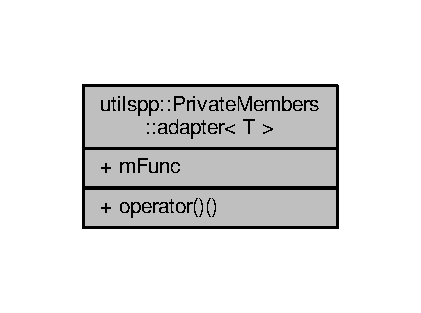
\includegraphics[width=202pt]{structutilspp_1_1PrivateMembers_1_1adapter__coll__graph}
\end{center}
\end{figure}
\subsection*{Public Member Functions}
\begin{DoxyCompactItemize}
\item 
\hypertarget{structutilspp_1_1PrivateMembers_1_1adapter_a2be7b2ab20c93e9c299a6eeeeb06d4d9}{void {\bfseries operator()} (T $\ast$)}\label{structutilspp_1_1PrivateMembers_1_1adapter_a2be7b2ab20c93e9c299a6eeeeb06d4d9}

\end{DoxyCompactItemize}
\subsection*{Public Attributes}
\begin{DoxyCompactItemize}
\item 
\hypertarget{structutilspp_1_1PrivateMembers_1_1adapter_ab8ad3f1f149b6e5ad4554a7c0d6718ad}{void($\ast$ {\bfseries m\-Func} )()}\label{structutilspp_1_1PrivateMembers_1_1adapter_ab8ad3f1f149b6e5ad4554a7c0d6718ad}

\end{DoxyCompactItemize}


The documentation for this struct was generated from the following files\-:\begin{DoxyCompactItemize}
\item 
include/utilspp/singleton/Private\-Members.\-hpp\item 
include/utilspp/singleton/Private\-Members.\-inl\end{DoxyCompactItemize}

\hypertarget{structutilspp_1_1tl_1_1append}{\section{utilspp\-:\-:tl\-:\-:append$<$ T\-List, T $>$ Struct Template Reference}
\label{structutilspp_1_1tl_1_1append}\index{utilspp\-::tl\-::append$<$ T\-List, T $>$@{utilspp\-::tl\-::append$<$ T\-List, T $>$}}
}


Collaboration diagram for utilspp\-:\-:tl\-:\-:append$<$ T\-List, T $>$\-:
\nopagebreak
\begin{figure}[H]
\begin{center}
\leavevmode
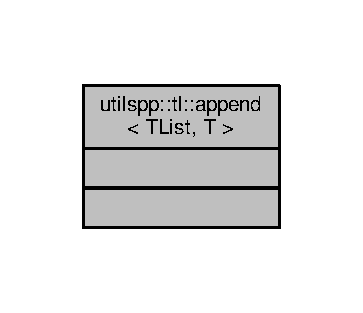
\includegraphics[width=174pt]{structutilspp_1_1tl_1_1append__coll__graph}
\end{center}
\end{figure}


The documentation for this struct was generated from the following file\-:\begin{DoxyCompactItemize}
\item 
include/utilspp/Type\-List.\-hpp\end{DoxyCompactItemize}

\hypertarget{structutilspp_1_1tl_1_1append_3_01NullType_00_01NullType_01_4}{\section{utilspp\-:\-:tl\-:\-:append$<$ Null\-Type, Null\-Type $>$ Struct Template Reference}
\label{structutilspp_1_1tl_1_1append_3_01NullType_00_01NullType_01_4}\index{utilspp\-::tl\-::append$<$ Null\-Type, Null\-Type $>$@{utilspp\-::tl\-::append$<$ Null\-Type, Null\-Type $>$}}
}


Collaboration diagram for utilspp\-:\-:tl\-:\-:append$<$ Null\-Type, Null\-Type $>$\-:\nopagebreak
\begin{figure}[H]
\begin{center}
\leavevmode
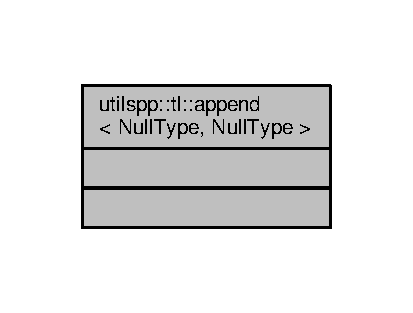
\includegraphics[width=198pt]{structutilspp_1_1tl_1_1append_3_01NullType_00_01NullType_01_4__coll__graph}
\end{center}
\end{figure}
\subsection*{Public Types}
\begin{DoxyCompactItemize}
\item 
\hypertarget{structutilspp_1_1tl_1_1append_3_01NullType_00_01NullType_01_4_a31a31ee2d8b5e3482cad92a628f8bff7}{typedef Null\-Type {\bfseries Result}}\label{structutilspp_1_1tl_1_1append_3_01NullType_00_01NullType_01_4_a31a31ee2d8b5e3482cad92a628f8bff7}

\end{DoxyCompactItemize}


The documentation for this struct was generated from the following file\-:\begin{DoxyCompactItemize}
\item 
include/utilspp/Type\-List.\-hpp\end{DoxyCompactItemize}

\hypertarget{structutilspp_1_1tl_1_1append_3_01NullType_00_01T_01_4}{\section{utilspp\-:\-:tl\-:\-:append$<$ Null\-Type, T $>$ Struct Template Reference}
\label{structutilspp_1_1tl_1_1append_3_01NullType_00_01T_01_4}\index{utilspp\-::tl\-::append$<$ Null\-Type, T $>$@{utilspp\-::tl\-::append$<$ Null\-Type, T $>$}}
}


Collaboration diagram for utilspp\-:\-:tl\-:\-:append$<$ Null\-Type, T $>$\-:\nopagebreak
\begin{figure}[H]
\begin{center}
\leavevmode
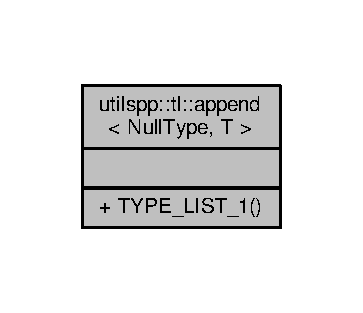
\includegraphics[width=174pt]{structutilspp_1_1tl_1_1append_3_01NullType_00_01T_01_4__coll__graph}
\end{center}
\end{figure}
\subsection*{Public Member Functions}
\begin{DoxyCompactItemize}
\item 
\hypertarget{structutilspp_1_1tl_1_1append_3_01NullType_00_01T_01_4_ac1e8e195f13a135885e3fdbcaf2dad96}{typedef {\bfseries T\-Y\-P\-E\-\_\-\-L\-I\-S\-T\-\_\-1} (T) Result}\label{structutilspp_1_1tl_1_1append_3_01NullType_00_01T_01_4_ac1e8e195f13a135885e3fdbcaf2dad96}

\end{DoxyCompactItemize}


The documentation for this struct was generated from the following file\-:\begin{DoxyCompactItemize}
\item 
include/utilspp/Type\-List.\-hpp\end{DoxyCompactItemize}

\hypertarget{structutilspp_1_1tl_1_1append_3_01NullType_00_01TypeList_3_01THead_00_01TTail_01_4_01_4}{\section{utilspp\-:\-:tl\-:\-:append$<$ Null\-Type, Type\-List$<$ T\-Head, T\-Tail $>$ $>$ Struct Template Reference}
\label{structutilspp_1_1tl_1_1append_3_01NullType_00_01TypeList_3_01THead_00_01TTail_01_4_01_4}\index{utilspp\-::tl\-::append$<$ Null\-Type, Type\-List$<$ T\-Head, T\-Tail $>$ $>$@{utilspp\-::tl\-::append$<$ Null\-Type, Type\-List$<$ T\-Head, T\-Tail $>$ $>$}}
}


Collaboration diagram for utilspp\-:\-:tl\-:\-:append$<$ Null\-Type, Type\-List$<$ T\-Head, T\-Tail $>$ $>$\-:
\nopagebreak
\begin{figure}[H]
\begin{center}
\leavevmode
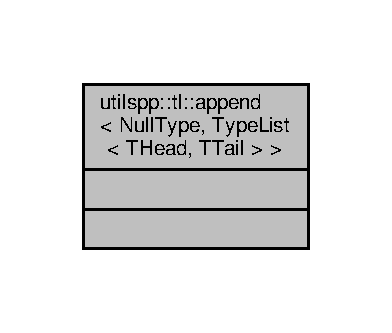
\includegraphics[width=188pt]{structutilspp_1_1tl_1_1append_3_01NullType_00_01TypeList_3_01THead_00_01TTail_01_4_01_4__coll__graph}
\end{center}
\end{figure}
\subsection*{Public Types}
\begin{DoxyCompactItemize}
\item 
\hypertarget{structutilspp_1_1tl_1_1append_3_01NullType_00_01TypeList_3_01THead_00_01TTail_01_4_01_4_a7e2cb7669f70b95cea96a76575ca934c}{typedef \hyperlink{structutilspp_1_1tl_1_1TypeList}{Type\-List}$<$ T\-Head, T\-Tail $>$ {\bfseries Result}}\label{structutilspp_1_1tl_1_1append_3_01NullType_00_01TypeList_3_01THead_00_01TTail_01_4_01_4_a7e2cb7669f70b95cea96a76575ca934c}

\end{DoxyCompactItemize}


The documentation for this struct was generated from the following file\-:\begin{DoxyCompactItemize}
\item 
include/utilspp/Type\-List.\-hpp\end{DoxyCompactItemize}

\hypertarget{structutilspp_1_1tl_1_1append_3_01TypeList_3_01THead_00_01TTail_01_4_00_01T_01_4}{\section{utilspp\-:\-:tl\-:\-:append$<$ Type\-List$<$ T\-Head, T\-Tail $>$, T $>$ Struct Template Reference}
\label{structutilspp_1_1tl_1_1append_3_01TypeList_3_01THead_00_01TTail_01_4_00_01T_01_4}\index{utilspp\-::tl\-::append$<$ Type\-List$<$ T\-Head, T\-Tail $>$, T $>$@{utilspp\-::tl\-::append$<$ Type\-List$<$ T\-Head, T\-Tail $>$, T $>$}}
}


Collaboration diagram for utilspp\-:\-:tl\-:\-:append$<$ Type\-List$<$ T\-Head, T\-Tail $>$, T $>$\-:\nopagebreak
\begin{figure}[H]
\begin{center}
\leavevmode
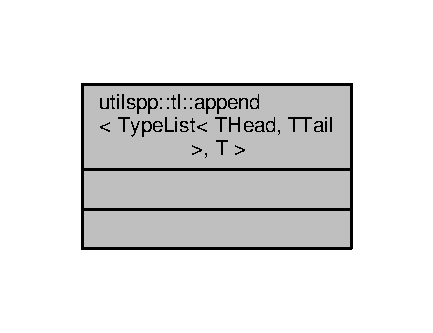
\includegraphics[width=208pt]{structutilspp_1_1tl_1_1append_3_01TypeList_3_01THead_00_01TTail_01_4_00_01T_01_4__coll__graph}
\end{center}
\end{figure}
\subsection*{Public Types}
\begin{DoxyCompactItemize}
\item 
\hypertarget{structutilspp_1_1tl_1_1append_3_01TypeList_3_01THead_00_01TTail_01_4_00_01T_01_4_af85ba63843e47eebcf0af6feeda0d295}{typedef \hyperlink{structutilspp_1_1tl_1_1TypeList}{Type\-List}$<$ T\-Head, \\*
typename \hyperlink{structutilspp_1_1tl_1_1append}{append}$<$ T\-Tail, T $>$\\*
\-::\hyperlink{structutilspp_1_1tl_1_1TypeList}{Result} $>$ {\bfseries Result}}\label{structutilspp_1_1tl_1_1append_3_01TypeList_3_01THead_00_01TTail_01_4_00_01T_01_4_af85ba63843e47eebcf0af6feeda0d295}

\end{DoxyCompactItemize}


The documentation for this struct was generated from the following file\-:\begin{DoxyCompactItemize}
\item 
include/utilspp/Type\-List.\-hpp\end{DoxyCompactItemize}

\hypertarget{classutilspp_1_1BinderFirst}{\section{utilspp\-:\-:Binder\-First$<$ Incoming $>$ Class Template Reference}
\label{classutilspp_1_1BinderFirst}\index{utilspp\-::\-Binder\-First$<$ Incoming $>$@{utilspp\-::\-Binder\-First$<$ Incoming $>$}}
}


Inheritance diagram for utilspp\-:\-:Binder\-First$<$ Incoming $>$\-:
\nopagebreak
\begin{figure}[H]
\begin{center}
\leavevmode
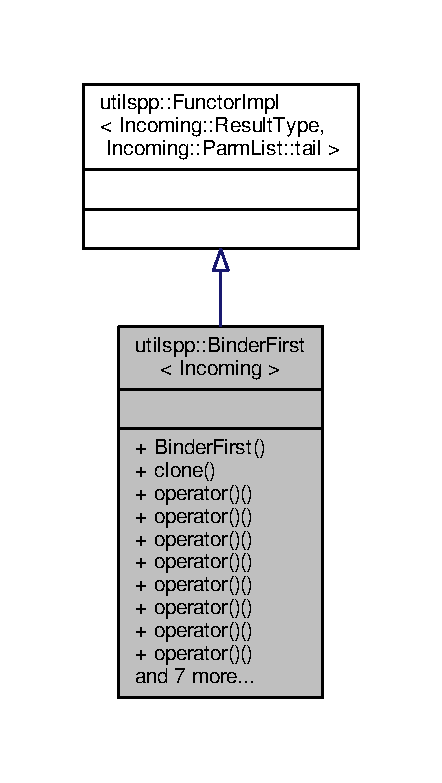
\includegraphics[width=212pt]{classutilspp_1_1BinderFirst__inherit__graph}
\end{center}
\end{figure}


Collaboration diagram for utilspp\-:\-:Binder\-First$<$ Incoming $>$\-:
\nopagebreak
\begin{figure}[H]
\begin{center}
\leavevmode
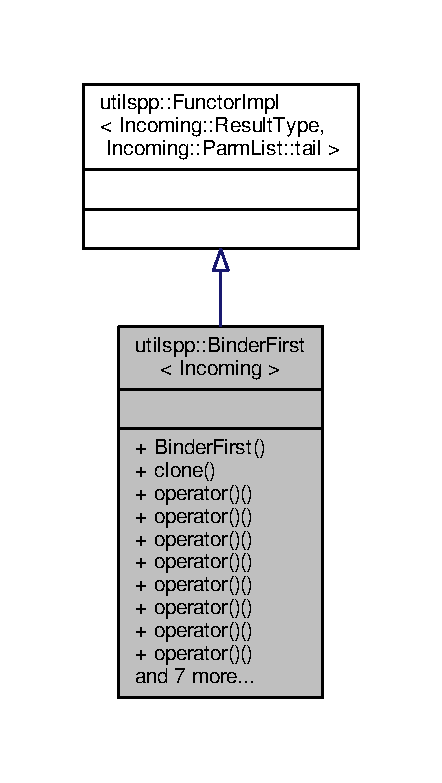
\includegraphics[width=212pt]{classutilspp_1_1BinderFirst__coll__graph}
\end{center}
\end{figure}
\subsection*{Public Member Functions}
\begin{DoxyCompactItemize}
\item 
\hypertarget{classutilspp_1_1BinderFirst_abfbd1c06cda97a041cd0847338bc8c17}{{\bfseries Binder\-First} (const Incoming \&fun, Bound bound)}\label{classutilspp_1_1BinderFirst_abfbd1c06cda97a041cd0847338bc8c17}

\item 
\hypertarget{classutilspp_1_1BinderFirst_a52db81ffa8bc5cb9aaaf5d79c2fdaf35}{\hyperlink{classutilspp_1_1BinderFirst}{Binder\-First} $\ast$ {\bfseries clone} () const }\label{classutilspp_1_1BinderFirst_a52db81ffa8bc5cb9aaaf5d79c2fdaf35}

\item 
\hypertarget{classutilspp_1_1BinderFirst_a7332050e7bb7b22d1d34d6b9021d5341}{Result\-Type {\bfseries operator()} ()}\label{classutilspp_1_1BinderFirst_a7332050e7bb7b22d1d34d6b9021d5341}

\item 
\hypertarget{classutilspp_1_1BinderFirst_a39130945d45a44a34e8d1e50e1ed155b}{Result\-Type {\bfseries operator()} (typename Outgoing\-::\-Parm1 p1)}\label{classutilspp_1_1BinderFirst_a39130945d45a44a34e8d1e50e1ed155b}

\item 
\hypertarget{classutilspp_1_1BinderFirst_ab87007390fce647f703058bb0490a69b}{Result\-Type {\bfseries operator()} (typename Outgoing\-::\-Parm1 p1, typename Outgoing\-::\-Parm2 p2)}\label{classutilspp_1_1BinderFirst_ab87007390fce647f703058bb0490a69b}

\item 
\hypertarget{classutilspp_1_1BinderFirst_a24be37c110ea7ced8aab8deb084d639e}{Result\-Type {\bfseries operator()} (typename Outgoing\-::\-Parm1 p1, typename Outgoing\-::\-Parm2 p2, typename Outgoing\-::\-Parm3 p3)}\label{classutilspp_1_1BinderFirst_a24be37c110ea7ced8aab8deb084d639e}

\item 
\hypertarget{classutilspp_1_1BinderFirst_a9245e530d25c19c1bfb7f4977762a0c1}{Result\-Type {\bfseries operator()} (typename Outgoing\-::\-Parm1 p1, typename Outgoing\-::\-Parm2 p2, typename Outgoing\-::\-Parm3 p3, typename Outgoing\-::\-Parm4 p4)}\label{classutilspp_1_1BinderFirst_a9245e530d25c19c1bfb7f4977762a0c1}

\item 
\hypertarget{classutilspp_1_1BinderFirst_af0f8eb10530c0faafd8b02facf4baa6d}{Result\-Type {\bfseries operator()} (typename Outgoing\-::\-Parm1 p1, typename Outgoing\-::\-Parm2 p2, typename Outgoing\-::\-Parm3 p3, typename Outgoing\-::\-Parm4 p4, typename Outgoing\-::\-Parm5 p5)}\label{classutilspp_1_1BinderFirst_af0f8eb10530c0faafd8b02facf4baa6d}

\item 
\hypertarget{classutilspp_1_1BinderFirst_ab413186751cda0cf7bf9f800f7a11672}{Result\-Type {\bfseries operator()} (typename Outgoing\-::\-Parm1 p1, typename Outgoing\-::\-Parm2 p2, typename Outgoing\-::\-Parm3 p3, typename Outgoing\-::\-Parm4 p4, typename Outgoing\-::\-Parm5 p5, typename Outgoing\-::\-Parm6 p6)}\label{classutilspp_1_1BinderFirst_ab413186751cda0cf7bf9f800f7a11672}

\item 
\hypertarget{classutilspp_1_1BinderFirst_a97b4cb9d2beced3402eced8cae8b8d45}{Result\-Type {\bfseries operator()} (typename Outgoing\-::\-Parm1 p1, typename Outgoing\-::\-Parm2 p2, typename Outgoing\-::\-Parm3 p3, typename Outgoing\-::\-Parm4 p4, typename Outgoing\-::\-Parm5 p5, typename Outgoing\-::\-Parm6 p6, typename Outgoing\-::\-Parm7 p7)}\label{classutilspp_1_1BinderFirst_a97b4cb9d2beced3402eced8cae8b8d45}

\item 
\hypertarget{classutilspp_1_1BinderFirst_adba1475c298df0c685b512f5ab839a93}{Result\-Type {\bfseries operator()} (typename Outgoing\-::\-Parm1 p1, typename Outgoing\-::\-Parm2 p2, typename Outgoing\-::\-Parm3 p3, typename Outgoing\-::\-Parm4 p4, typename Outgoing\-::\-Parm5 p5, typename Outgoing\-::\-Parm6 p6, typename Outgoing\-::\-Parm7 p7, typename Outgoing\-::\-Parm8 p8)}\label{classutilspp_1_1BinderFirst_adba1475c298df0c685b512f5ab839a93}

\item 
\hypertarget{classutilspp_1_1BinderFirst_a190a42dd2376ad4a7c3a8bfba0a0ef3f}{Result\-Type {\bfseries operator()} (typename Outgoing\-::\-Parm1 p1, typename Outgoing\-::\-Parm2 p2, typename Outgoing\-::\-Parm3 p3, typename Outgoing\-::\-Parm4 p4, typename Outgoing\-::\-Parm5 p5, typename Outgoing\-::\-Parm6 p6, typename Outgoing\-::\-Parm7 p7, typename Outgoing\-::\-Parm8 p8, typename Outgoing\-::\-Parm9 p9)}\label{classutilspp_1_1BinderFirst_a190a42dd2376ad4a7c3a8bfba0a0ef3f}

\item 
\hypertarget{classutilspp_1_1BinderFirst_adbc946ab09fb1e5d0937e65a1b4ba4d8}{Result\-Type {\bfseries operator()} (typename Outgoing\-::\-Parm1 p1, typename Outgoing\-::\-Parm2 p2, typename Outgoing\-::\-Parm3 p3, typename Outgoing\-::\-Parm4 p4, typename Outgoing\-::\-Parm5 p5, typename Outgoing\-::\-Parm6 p6, typename Outgoing\-::\-Parm7 p7, typename Outgoing\-::\-Parm8 p8, typename Outgoing\-::\-Parm9 p9, typename Outgoing\-::\-Parm10 p10)}\label{classutilspp_1_1BinderFirst_adbc946ab09fb1e5d0937e65a1b4ba4d8}

\item 
\hypertarget{classutilspp_1_1BinderFirst_a7c7decc3240563eb2df479b627a90cf1}{Result\-Type {\bfseries operator()} (typename Outgoing\-::\-Parm1 p1, typename Outgoing\-::\-Parm2 p2, typename Outgoing\-::\-Parm3 p3, typename Outgoing\-::\-Parm4 p4, typename Outgoing\-::\-Parm5 p5, typename Outgoing\-::\-Parm6 p6, typename Outgoing\-::\-Parm7 p7, typename Outgoing\-::\-Parm8 p8, typename Outgoing\-::\-Parm9 p9, typename Outgoing\-::\-Parm10 p10, typename Outgoing\-::\-Parm11 p11)}\label{classutilspp_1_1BinderFirst_a7c7decc3240563eb2df479b627a90cf1}

\item 
\hypertarget{classutilspp_1_1BinderFirst_a7ae7e7c68f34f42dc0029c37abc0a349}{Result\-Type {\bfseries operator()} (typename Outgoing\-::\-Parm1 p1, typename Outgoing\-::\-Parm2 p2, typename Outgoing\-::\-Parm3 p3, typename Outgoing\-::\-Parm4 p4, typename Outgoing\-::\-Parm5 p5, typename Outgoing\-::\-Parm6 p6, typename Outgoing\-::\-Parm7 p7, typename Outgoing\-::\-Parm8 p8, typename Outgoing\-::\-Parm9 p9, typename Outgoing\-::\-Parm10 p10, typename Outgoing\-::\-Parm11 p11, typename Outgoing\-::\-Parm12 p12)}\label{classutilspp_1_1BinderFirst_a7ae7e7c68f34f42dc0029c37abc0a349}

\item 
\hypertarget{classutilspp_1_1BinderFirst_a3db2a8159433982942440934afbdac3e}{Result\-Type {\bfseries operator()} (typename Outgoing\-::\-Parm1 p1, typename Outgoing\-::\-Parm2 p2, typename Outgoing\-::\-Parm3 p3, typename Outgoing\-::\-Parm4 p4, typename Outgoing\-::\-Parm5 p5, typename Outgoing\-::\-Parm6 p6, typename Outgoing\-::\-Parm7 p7, typename Outgoing\-::\-Parm8 p8, typename Outgoing\-::\-Parm9 p9, typename Outgoing\-::\-Parm10 p10, typename Outgoing\-::\-Parm11 p11, typename Outgoing\-::\-Parm12 p12, typename Outgoing\-::\-Parm13 p13)}\label{classutilspp_1_1BinderFirst_a3db2a8159433982942440934afbdac3e}

\item 
\hypertarget{classutilspp_1_1BinderFirst_adc155e1796230468a729ee2103819d1e}{Result\-Type {\bfseries operator()} (typename Outgoing\-::\-Parm1 p1, typename Outgoing\-::\-Parm2 p2, typename Outgoing\-::\-Parm3 p3, typename Outgoing\-::\-Parm4 p4, typename Outgoing\-::\-Parm5 p5, typename Outgoing\-::\-Parm6 p6, typename Outgoing\-::\-Parm7 p7, typename Outgoing\-::\-Parm8 p8, typename Outgoing\-::\-Parm9 p9, typename Outgoing\-::\-Parm10 p10, typename Outgoing\-::\-Parm11 p11, typename Outgoing\-::\-Parm12 p12, typename Outgoing\-::\-Parm13 p13, typename Outgoing\-::\-Parm14 p14)}\label{classutilspp_1_1BinderFirst_adc155e1796230468a729ee2103819d1e}

\end{DoxyCompactItemize}


The documentation for this class was generated from the following file\-:\begin{DoxyCompactItemize}
\item 
include/utilspp/functor/Binder.\-hpp\end{DoxyCompactItemize}

\hypertarget{classcurlpp_1_1CallbackException}{\section{curlpp\-:\-:Callback\-Exception$<$ Exception\-Type $>$ Class Template Reference}
\label{classcurlpp_1_1CallbackException}\index{curlpp\-::\-Callback\-Exception$<$ Exception\-Type $>$@{curlpp\-::\-Callback\-Exception$<$ Exception\-Type $>$}}
}


This exception is thrown by the curlpp\-::raise\-Exception function.  




{\ttfamily \#include $<$Exception.\-hpp$>$}



Inheritance diagram for curlpp\-:\-:Callback\-Exception$<$ Exception\-Type $>$\-:\nopagebreak
\begin{figure}[H]
\begin{center}
\leavevmode
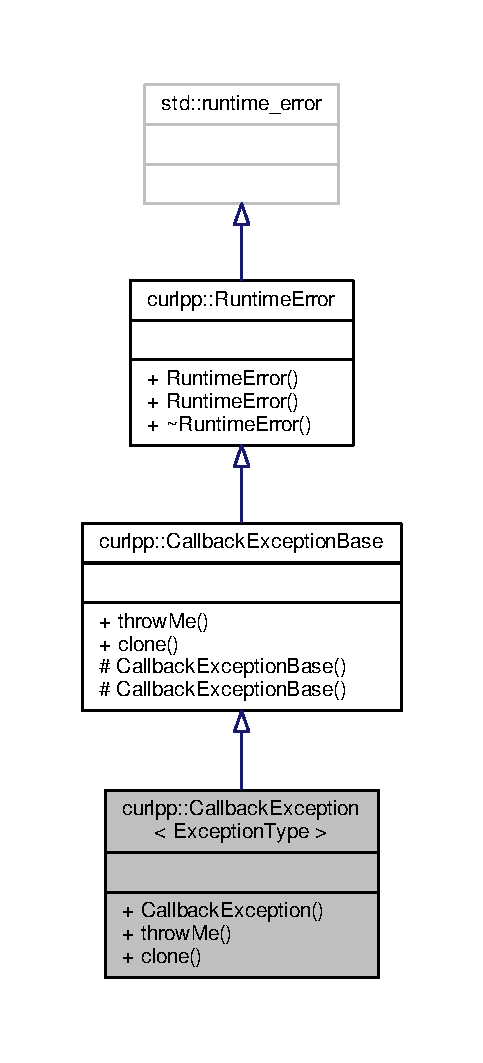
\includegraphics[width=232pt]{classcurlpp_1_1CallbackException__inherit__graph}
\end{center}
\end{figure}


Collaboration diagram for curlpp\-:\-:Callback\-Exception$<$ Exception\-Type $>$\-:\nopagebreak
\begin{figure}[H]
\begin{center}
\leavevmode
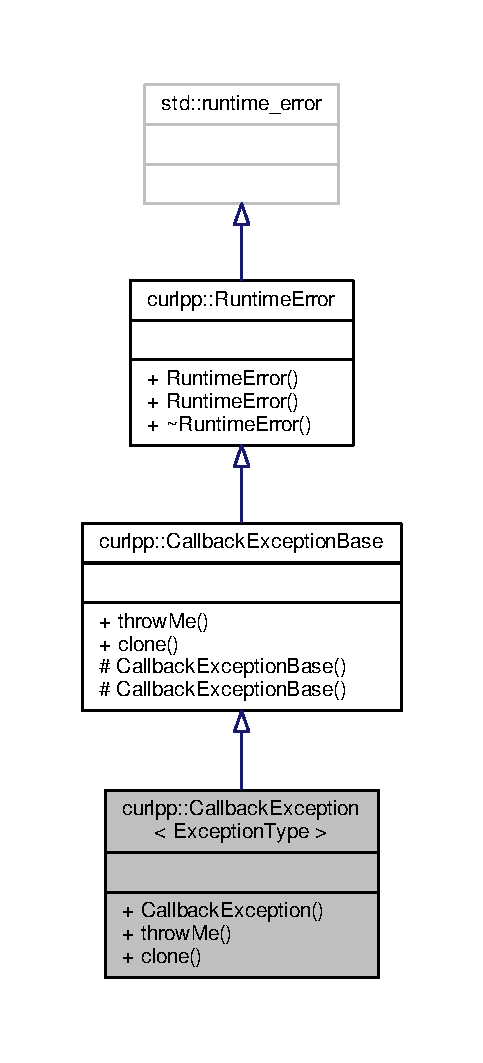
\includegraphics[width=232pt]{classcurlpp_1_1CallbackException__coll__graph}
\end{center}
\end{figure}
\subsection*{Public Types}
\begin{DoxyCompactItemize}
\item 
\hypertarget{classcurlpp_1_1CallbackException_a14c78c379d35648c686fbcebee24b678}{typedef \hyperlink{classcurlpp_1_1CallbackException}{Callback\-Exception}\\*
$<$ Exception\-Type $>$ {\bfseries \-\_\-\-C\-E}}\label{classcurlpp_1_1CallbackException_a14c78c379d35648c686fbcebee24b678}

\end{DoxyCompactItemize}
\subsection*{Public Member Functions}
\begin{DoxyCompactItemize}
\item 
\hypertarget{classcurlpp_1_1CallbackException_a9594d36ed3921cafcd50b1186ba9a31d}{{\bfseries Callback\-Exception} (const Exception\-Type \&e)}\label{classcurlpp_1_1CallbackException_a9594d36ed3921cafcd50b1186ba9a31d}

\item 
\hypertarget{classcurlpp_1_1CallbackException_a2d29d21f7a15e8bd785269d1309c9cee}{virtual void {\bfseries throw\-Me} ()}\label{classcurlpp_1_1CallbackException_a2d29d21f7a15e8bd785269d1309c9cee}

\item 
\hypertarget{classcurlpp_1_1CallbackException_a64eb25a75d04ee77cc0664885305de6a}{virtual \hyperlink{classcurlpp_1_1CallbackException}{\-\_\-\-C\-E} $\ast$ {\bfseries clone} ()}\label{classcurlpp_1_1CallbackException_a64eb25a75d04ee77cc0664885305de6a}

\end{DoxyCompactItemize}
\subsection*{Additional Inherited Members}


\subsection{Detailed Description}
\subsubsection*{template$<$typename Exception\-Type$>$class curlpp\-::\-Callback\-Exception$<$ Exception\-Type $>$}

This exception is thrown by the curlpp\-::raise\-Exception function. 

It's used to throw exceptions within callbacks 

The documentation for this class was generated from the following file\-:\begin{DoxyCompactItemize}
\item 
include/curlpp/Exception.\-hpp\end{DoxyCompactItemize}

\hypertarget{classcurlpp_1_1CallbackExceptionBase}{\section{curlpp\-:\-:Callback\-Exception\-Base Class Reference}
\label{classcurlpp_1_1CallbackExceptionBase}\index{curlpp\-::\-Callback\-Exception\-Base@{curlpp\-::\-Callback\-Exception\-Base}}
}


This exception is thrown by the curlpp\-::raise\-Exception function.  




{\ttfamily \#include $<$Exception.\-hpp$>$}



Inheritance diagram for curlpp\-:\-:Callback\-Exception\-Base\-:\nopagebreak
\begin{figure}[H]
\begin{center}
\leavevmode
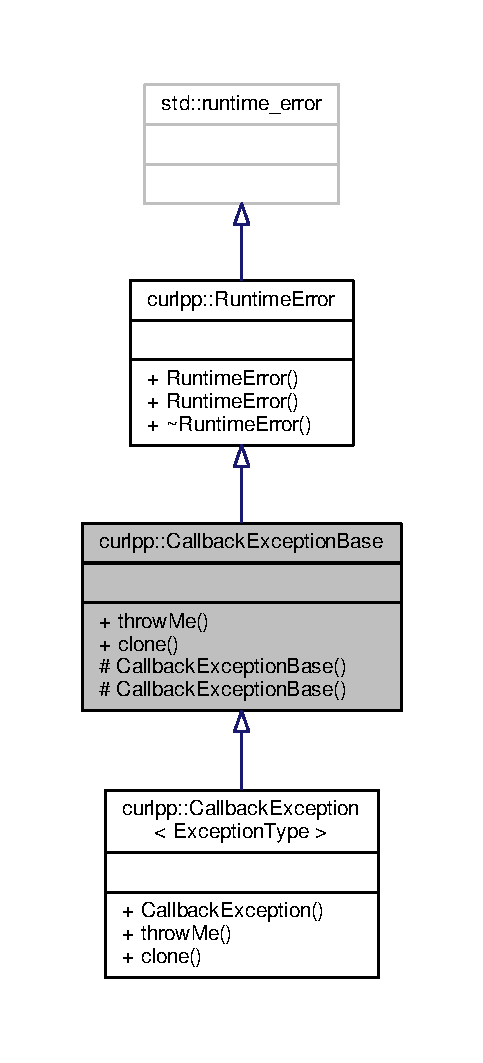
\includegraphics[width=232pt]{classcurlpp_1_1CallbackExceptionBase__inherit__graph}
\end{center}
\end{figure}


Collaboration diagram for curlpp\-:\-:Callback\-Exception\-Base\-:\nopagebreak
\begin{figure}[H]
\begin{center}
\leavevmode
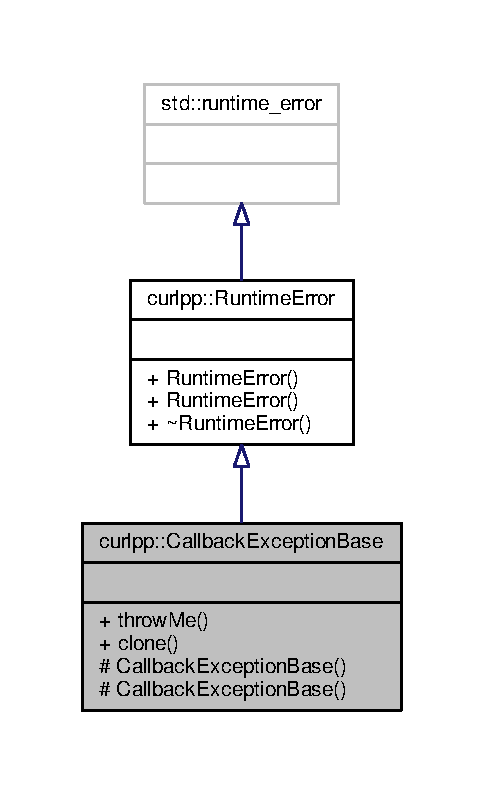
\includegraphics[width=232pt]{classcurlpp_1_1CallbackExceptionBase__coll__graph}
\end{center}
\end{figure}
\subsection*{Public Member Functions}
\begin{DoxyCompactItemize}
\item 
\hypertarget{classcurlpp_1_1CallbackExceptionBase_a4fd828e9866ed8bc914051738c530d8f}{virtual void {\bfseries throw\-Me} ()=0}\label{classcurlpp_1_1CallbackExceptionBase_a4fd828e9866ed8bc914051738c530d8f}

\item 
\hypertarget{classcurlpp_1_1CallbackExceptionBase_a9bdb8d529c717cdb1055ab65b38a4912}{virtual \hyperlink{classcurlpp_1_1CallbackExceptionBase}{Callback\-Exception\-Base} $\ast$ {\bfseries clone} ()=0}\label{classcurlpp_1_1CallbackExceptionBase_a9bdb8d529c717cdb1055ab65b38a4912}

\end{DoxyCompactItemize}
\subsection*{Protected Member Functions}
\begin{DoxyCompactItemize}
\item 
\hypertarget{classcurlpp_1_1CallbackExceptionBase_a31a83304a2506ac7b6723d85a4744047}{{\bfseries Callback\-Exception\-Base} (const \hyperlink{classcurlpp_1_1CallbackExceptionBase}{Callback\-Exception\-Base} \&other)}\label{classcurlpp_1_1CallbackExceptionBase_a31a83304a2506ac7b6723d85a4744047}

\end{DoxyCompactItemize}


\subsection{Detailed Description}
This exception is thrown by the curlpp\-::raise\-Exception function. 

It's used to throw exceptions within callbacks 

The documentation for this class was generated from the following files\-:\begin{DoxyCompactItemize}
\item 
include/curlpp/Exception.\-hpp\item 
src/curlpp/Exception.\-cpp\end{DoxyCompactItemize}

\hypertarget{structcurlpp_1_1internal_1_1Callbacks}{\section{curlpp\-:\-:internal\-:\-:Callbacks Struct Reference}
\label{structcurlpp_1_1internal_1_1Callbacks}\index{curlpp\-::internal\-::\-Callbacks@{curlpp\-::internal\-::\-Callbacks}}
}


Collaboration diagram for curlpp\-:\-:internal\-:\-:Callbacks\-:
\nopagebreak
\begin{figure}[H]
\begin{center}
\leavevmode
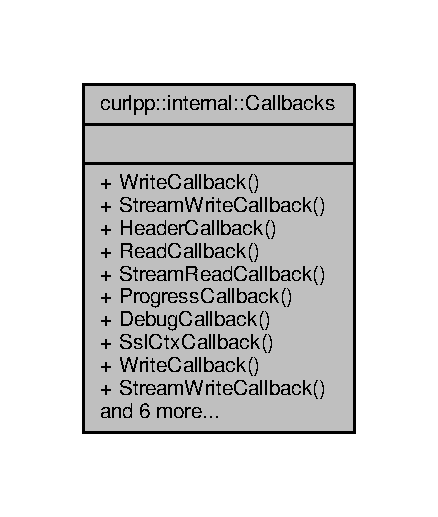
\includegraphics[width=210pt]{structcurlpp_1_1internal_1_1Callbacks__coll__graph}
\end{center}
\end{figure}
\subsection*{Static Public Member Functions}
\begin{DoxyCompactItemize}
\item 
\hypertarget{structcurlpp_1_1internal_1_1Callbacks_a5f1b4922a3f68892d25db51bcce627b3}{static size\-\_\-t {\bfseries Write\-Callback} (char $\ast$buffer, size\-\_\-t size, size\-\_\-t nitems, \hyperlink{classcurlpp_1_1internal_1_1CurlHandle}{internal\-::\-Curl\-Handle} $\ast$handle)}\label{structcurlpp_1_1internal_1_1Callbacks_a5f1b4922a3f68892d25db51bcce627b3}

\item 
\hypertarget{structcurlpp_1_1internal_1_1Callbacks_a68277a58922263611d75cb146fd58801}{static size\-\_\-t {\bfseries Stream\-Write\-Callback} (char $\ast$buffer, size\-\_\-t size, size\-\_\-t nitems, std\-::ostream $\ast$stream)}\label{structcurlpp_1_1internal_1_1Callbacks_a68277a58922263611d75cb146fd58801}

\item 
\hypertarget{structcurlpp_1_1internal_1_1Callbacks_a8297769942b956c1d265064ee1327665}{static size\-\_\-t {\bfseries Header\-Callback} (char $\ast$buffer, size\-\_\-t size, size\-\_\-t nitems, \hyperlink{classcurlpp_1_1internal_1_1CurlHandle}{internal\-::\-Curl\-Handle} $\ast$handle)}\label{structcurlpp_1_1internal_1_1Callbacks_a8297769942b956c1d265064ee1327665}

\item 
\hypertarget{structcurlpp_1_1internal_1_1Callbacks_a7eda5772a5a9c54fc1a2c1360bcc941d}{static size\-\_\-t {\bfseries Read\-Callback} (char $\ast$buffer, size\-\_\-t size, size\-\_\-t nitems, \hyperlink{classcurlpp_1_1internal_1_1CurlHandle}{internal\-::\-Curl\-Handle} $\ast$handle)}\label{structcurlpp_1_1internal_1_1Callbacks_a7eda5772a5a9c54fc1a2c1360bcc941d}

\item 
\hypertarget{structcurlpp_1_1internal_1_1Callbacks_a7ab93128d1b912af0fac7a3845768eed}{static size\-\_\-t {\bfseries Stream\-Read\-Callback} (char $\ast$buffer, size\-\_\-t size, size\-\_\-t nitems, std\-::istream $\ast$stream)}\label{structcurlpp_1_1internal_1_1Callbacks_a7ab93128d1b912af0fac7a3845768eed}

\item 
\hypertarget{structcurlpp_1_1internal_1_1Callbacks_aca7773bc439f657959311f11f73b1396}{static int {\bfseries Progress\-Callback} (\hyperlink{classcurlpp_1_1internal_1_1CurlHandle}{internal\-::\-Curl\-Handle} $\ast$handle, double dltotal, double dlnow, double ultotal, double ulnow)}\label{structcurlpp_1_1internal_1_1Callbacks_aca7773bc439f657959311f11f73b1396}

\item 
\hypertarget{structcurlpp_1_1internal_1_1Callbacks_ab09b4081b01ef53c602643b68c7c3ddb}{static int {\bfseries Debug\-Callback} (C\-U\-R\-L $\ast$, curl\-\_\-infotype type, char $\ast$data, size\-\_\-t size, \hyperlink{classcurlpp_1_1internal_1_1CurlHandle}{internal\-::\-Curl\-Handle} $\ast$handle)}\label{structcurlpp_1_1internal_1_1Callbacks_ab09b4081b01ef53c602643b68c7c3ddb}

\item 
\hypertarget{structcurlpp_1_1internal_1_1Callbacks_ad62a0abad12fb7d3e25ead35b500973a}{static C\-U\-R\-Lcode {\bfseries Ssl\-Ctx\-Callback} (C\-U\-R\-L $\ast$, void $\ast$ssl\-\_\-ctx, \hyperlink{classcurlpp_1_1internal_1_1CurlHandle}{internal\-::\-Curl\-Handle} $\ast$handle)}\label{structcurlpp_1_1internal_1_1Callbacks_ad62a0abad12fb7d3e25ead35b500973a}

\item 
\hypertarget{structcurlpp_1_1internal_1_1Callbacks_a5f1b4922a3f68892d25db51bcce627b3}{static size\-\_\-t {\bfseries Write\-Callback} (char $\ast$buffer, size\-\_\-t size, size\-\_\-t nitems, \hyperlink{classcurlpp_1_1internal_1_1CurlHandle}{internal\-::\-Curl\-Handle} $\ast$handle)}\label{structcurlpp_1_1internal_1_1Callbacks_a5f1b4922a3f68892d25db51bcce627b3}

\item 
\hypertarget{structcurlpp_1_1internal_1_1Callbacks_a68277a58922263611d75cb146fd58801}{static size\-\_\-t {\bfseries Stream\-Write\-Callback} (char $\ast$buffer, size\-\_\-t size, size\-\_\-t nitems, std\-::ostream $\ast$stream)}\label{structcurlpp_1_1internal_1_1Callbacks_a68277a58922263611d75cb146fd58801}

\item 
\hypertarget{structcurlpp_1_1internal_1_1Callbacks_a8297769942b956c1d265064ee1327665}{static size\-\_\-t {\bfseries Header\-Callback} (char $\ast$buffer, size\-\_\-t size, size\-\_\-t nitems, \hyperlink{classcurlpp_1_1internal_1_1CurlHandle}{internal\-::\-Curl\-Handle} $\ast$handle)}\label{structcurlpp_1_1internal_1_1Callbacks_a8297769942b956c1d265064ee1327665}

\item 
\hypertarget{structcurlpp_1_1internal_1_1Callbacks_a7eda5772a5a9c54fc1a2c1360bcc941d}{static size\-\_\-t {\bfseries Read\-Callback} (char $\ast$buffer, size\-\_\-t size, size\-\_\-t nitems, \hyperlink{classcurlpp_1_1internal_1_1CurlHandle}{internal\-::\-Curl\-Handle} $\ast$handle)}\label{structcurlpp_1_1internal_1_1Callbacks_a7eda5772a5a9c54fc1a2c1360bcc941d}

\item 
\hypertarget{structcurlpp_1_1internal_1_1Callbacks_a7ab93128d1b912af0fac7a3845768eed}{static size\-\_\-t {\bfseries Stream\-Read\-Callback} (char $\ast$buffer, size\-\_\-t size, size\-\_\-t nitems, std\-::istream $\ast$stream)}\label{structcurlpp_1_1internal_1_1Callbacks_a7ab93128d1b912af0fac7a3845768eed}

\item 
\hypertarget{structcurlpp_1_1internal_1_1Callbacks_aca7773bc439f657959311f11f73b1396}{static int {\bfseries Progress\-Callback} (\hyperlink{classcurlpp_1_1internal_1_1CurlHandle}{internal\-::\-Curl\-Handle} $\ast$handle, double dltotal, double dlnow, double ultotal, double ulnow)}\label{structcurlpp_1_1internal_1_1Callbacks_aca7773bc439f657959311f11f73b1396}

\item 
\hypertarget{structcurlpp_1_1internal_1_1Callbacks_ab09b4081b01ef53c602643b68c7c3ddb}{static int {\bfseries Debug\-Callback} (C\-U\-R\-L $\ast$, curl\-\_\-infotype type, char $\ast$data, size\-\_\-t size, \hyperlink{classcurlpp_1_1internal_1_1CurlHandle}{internal\-::\-Curl\-Handle} $\ast$handle)}\label{structcurlpp_1_1internal_1_1Callbacks_ab09b4081b01ef53c602643b68c7c3ddb}

\item 
\hypertarget{structcurlpp_1_1internal_1_1Callbacks_ad62a0abad12fb7d3e25ead35b500973a}{static C\-U\-R\-Lcode {\bfseries Ssl\-Ctx\-Callback} (C\-U\-R\-L $\ast$, void $\ast$ssl\-\_\-ctx, \hyperlink{classcurlpp_1_1internal_1_1CurlHandle}{internal\-::\-Curl\-Handle} $\ast$handle)}\label{structcurlpp_1_1internal_1_1Callbacks_ad62a0abad12fb7d3e25ead35b500973a}

\end{DoxyCompactItemize}


The documentation for this struct was generated from the following file\-:\begin{DoxyCompactItemize}
\item 
src/curlpp/internal/Option\-Setter.\-cpp\end{DoxyCompactItemize}

\hypertarget{classcurlpp_1_1Cleanup}{\section{curlpp\-:\-:Cleanup Class Reference}
\label{classcurlpp_1_1Cleanup}\index{curlpp\-::\-Cleanup@{curlpp\-::\-Cleanup}}
}


This is an obsolete class.  




{\ttfamily \#include $<$c\-U\-R\-Lpp.\-hpp$>$}



Collaboration diagram for curlpp\-:\-:Cleanup\-:
\nopagebreak
\begin{figure}[H]
\begin{center}
\leavevmode
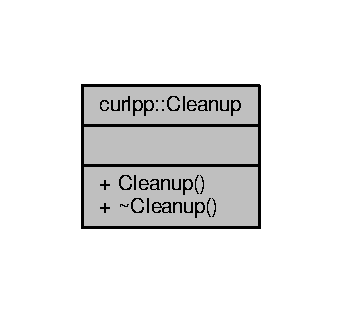
\includegraphics[width=164pt]{classcurlpp_1_1Cleanup__coll__graph}
\end{center}
\end{figure}


\subsection{Detailed Description}
This is an obsolete class. 

D\-O N\-O\-T use it.

The only reason it's still here, is to be sure that it is backward compatible. This class was taking care of initialization and cleaning up curlpp (also libc\-U\-R\-L) (it was calling curlpp\-:terminate() in his destructor). However, from now on, you do not need this class. Note that the removal of this class was done because it was raising some threading issues.

Old documentation of that class\-:

If you want to be sure that curlpp is cleaned up after you reached the end of scope of a specific function using curlpp, instantiate this class. This function call curlpp\-::initialize() in his constructor, so you don't have to call it by yourself, when you have decided to use it.

See curlpp\-::initialize(long flags) and curlpp\-:terminate() for more documentation. 

The documentation for this class was generated from the following files\-:\begin{DoxyCompactItemize}
\item 
include/curlpp/c\-U\-R\-Lpp.\-hpp\item 
src/curlpp/c\-U\-R\-Lpp.\-cpp\end{DoxyCompactItemize}

\hypertarget{classutilspp_1_1clone__ptr}{\section{utilspp\-:\-:clone\-\_\-ptr$<$ T $>$ Class Template Reference}
\label{classutilspp_1_1clone__ptr}\index{utilspp\-::clone\-\_\-ptr$<$ T $>$@{utilspp\-::clone\-\_\-ptr$<$ T $>$}}
}


Collaboration diagram for utilspp\-:\-:clone\-\_\-ptr$<$ T $>$\-:
\nopagebreak
\begin{figure}[H]
\begin{center}
\leavevmode
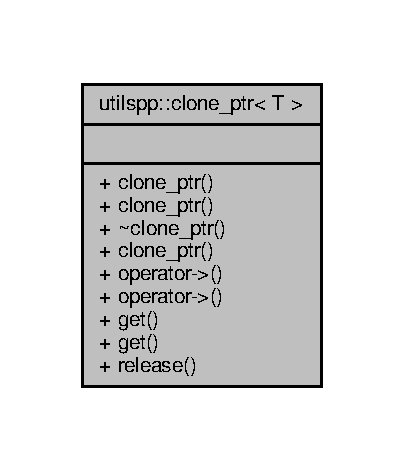
\includegraphics[width=194pt]{classutilspp_1_1clone__ptr__coll__graph}
\end{center}
\end{figure}
\subsection*{Public Member Functions}
\begin{DoxyCompactItemize}
\item 
\hypertarget{classutilspp_1_1clone__ptr_adb07a3d88bef21f8c446a15180037cff}{{\bfseries clone\-\_\-ptr} (T $\ast$value)}\label{classutilspp_1_1clone__ptr_adb07a3d88bef21f8c446a15180037cff}

\item 
\hypertarget{classutilspp_1_1clone__ptr_a67f01cdd8cd0bd0b215ba1c56d59b4c5}{{\bfseries clone\-\_\-ptr} (const \hyperlink{classutilspp_1_1clone__ptr}{clone\-\_\-ptr} \&other)}\label{classutilspp_1_1clone__ptr_a67f01cdd8cd0bd0b215ba1c56d59b4c5}

\item 
\hypertarget{classutilspp_1_1clone__ptr_a076ae7fd6fbea7f96c840e0f82919f05}{T $\ast$ {\bfseries operator-\/$>$} ()}\label{classutilspp_1_1clone__ptr_a076ae7fd6fbea7f96c840e0f82919f05}

\item 
\hypertarget{classutilspp_1_1clone__ptr_a68cc19aecaed2963ae4a0208ab31f19b}{const T $\ast$ {\bfseries operator-\/$>$} () const }\label{classutilspp_1_1clone__ptr_a68cc19aecaed2963ae4a0208ab31f19b}

\item 
\hypertarget{classutilspp_1_1clone__ptr_a90a155df754cd98da6b24a2e9c3946ec}{T $\ast$ {\bfseries get} ()}\label{classutilspp_1_1clone__ptr_a90a155df754cd98da6b24a2e9c3946ec}

\item 
\hypertarget{classutilspp_1_1clone__ptr_ad55d16d5ada4a014219c0141210d1dc4}{const T $\ast$ {\bfseries get} () const }\label{classutilspp_1_1clone__ptr_ad55d16d5ada4a014219c0141210d1dc4}

\item 
\hypertarget{classutilspp_1_1clone__ptr_ad1e37406c84cbcb27267f0d170b1958f}{T $\ast$ {\bfseries release} ()}\label{classutilspp_1_1clone__ptr_ad1e37406c84cbcb27267f0d170b1958f}

\end{DoxyCompactItemize}


The documentation for this class was generated from the following file\-:\begin{DoxyCompactItemize}
\item 
include/utilspp/clone\-\_\-ptr.\-hpp\end{DoxyCompactItemize}

\hypertarget{classutilspp_1_1PrivateMembers_1_1ConcreteLifetimeTracker}{\section{utilspp\-:\-:Private\-Members\-:\-:Concrete\-Lifetime\-Tracker$<$ T, T\-Destroyer $>$ Class Template Reference}
\label{classutilspp_1_1PrivateMembers_1_1ConcreteLifetimeTracker}\index{utilspp\-::\-Private\-Members\-::\-Concrete\-Lifetime\-Tracker$<$ T, T\-Destroyer $>$@{utilspp\-::\-Private\-Members\-::\-Concrete\-Lifetime\-Tracker$<$ T, T\-Destroyer $>$}}
}


Concrete lifetime tracker for objects of type T.  




{\ttfamily \#include $<$Private\-Members.\-hpp$>$}



Inheritance diagram for utilspp\-:\-:Private\-Members\-:\-:Concrete\-Lifetime\-Tracker$<$ T, T\-Destroyer $>$\-:
\nopagebreak
\begin{figure}[H]
\begin{center}
\leavevmode
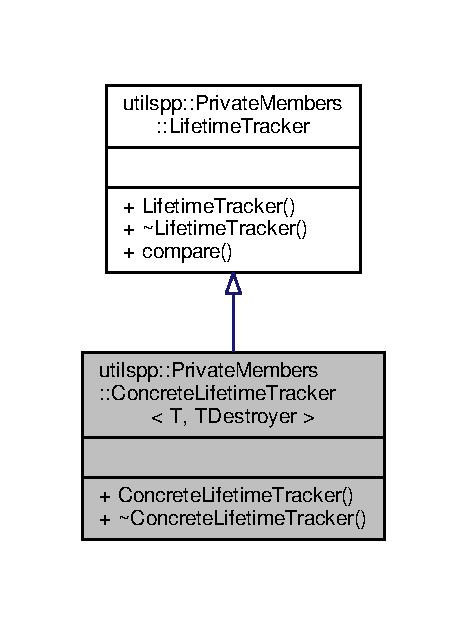
\includegraphics[width=224pt]{classutilspp_1_1PrivateMembers_1_1ConcreteLifetimeTracker__inherit__graph}
\end{center}
\end{figure}


Collaboration diagram for utilspp\-:\-:Private\-Members\-:\-:Concrete\-Lifetime\-Tracker$<$ T, T\-Destroyer $>$\-:
\nopagebreak
\begin{figure}[H]
\begin{center}
\leavevmode
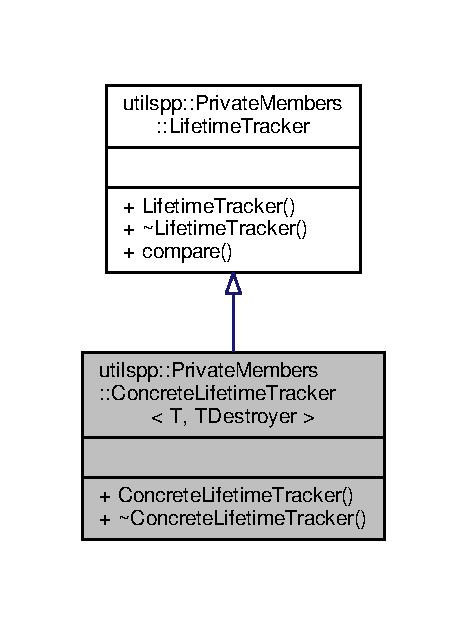
\includegraphics[width=224pt]{classutilspp_1_1PrivateMembers_1_1ConcreteLifetimeTracker__coll__graph}
\end{center}
\end{figure}
\subsection*{Public Member Functions}
\begin{DoxyCompactItemize}
\item 
\hypertarget{classutilspp_1_1PrivateMembers_1_1ConcreteLifetimeTracker_af560d6aa684c50ae7bfb533fd6ac739c}{{\bfseries Concrete\-Lifetime\-Tracker} (T $\ast$obj, unsigned int longevity, T\-Destroyer d)}\label{classutilspp_1_1PrivateMembers_1_1ConcreteLifetimeTracker_af560d6aa684c50ae7bfb533fd6ac739c}

\end{DoxyCompactItemize}
\subsection*{Additional Inherited Members}


\subsection{Detailed Description}
\subsubsection*{template$<$typename T, typename T\-Destroyer$>$class utilspp\-::\-Private\-Members\-::\-Concrete\-Lifetime\-Tracker$<$ T, T\-Destroyer $>$}

Concrete lifetime tracker for objects of type T. 

The documentation for this class was generated from the following files\-:\begin{DoxyCompactItemize}
\item 
include/utilspp/singleton/Private\-Members.\-hpp\item 
include/utilspp/singleton/Private\-Members.\-inl\end{DoxyCompactItemize}

\hypertarget{classcurlpp_1_1FormParts_1_1Content}{\section{curlpp\-:\-:Form\-Parts\-:\-:Content Class Reference}
\label{classcurlpp_1_1FormParts_1_1Content}\index{curlpp\-::\-Form\-Parts\-::\-Content@{curlpp\-::\-Form\-Parts\-::\-Content}}
}


This class is a file post.  




{\ttfamily \#include $<$Form.\-hpp$>$}



Inheritance diagram for curlpp\-:\-:Form\-Parts\-:\-:Content\-:\nopagebreak
\begin{figure}[H]
\begin{center}
\leavevmode
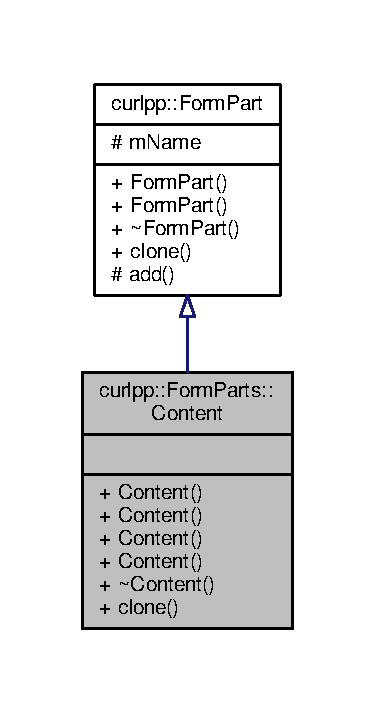
\includegraphics[width=180pt]{classcurlpp_1_1FormParts_1_1Content__inherit__graph}
\end{center}
\end{figure}


Collaboration diagram for curlpp\-:\-:Form\-Parts\-:\-:Content\-:\nopagebreak
\begin{figure}[H]
\begin{center}
\leavevmode
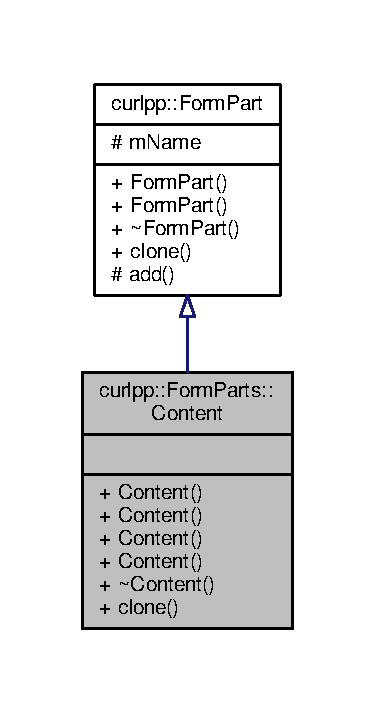
\includegraphics[width=180pt]{classcurlpp_1_1FormParts_1_1Content__coll__graph}
\end{center}
\end{figure}
\subsection*{Public Member Functions}
\begin{DoxyCompactItemize}
\item 
\hyperlink{classcurlpp_1_1FormParts_1_1Content_af3320998888d4c4fc85cd86f5c45efd1}{Content} (const char $\ast$name, const char $\ast$content)
\begin{DoxyCompactList}\small\item\em initialize a \hyperlink{classcurlpp_1_1FormParts_1_1Content}{Content} part. \end{DoxyCompactList}\item 
\hyperlink{classcurlpp_1_1FormParts_1_1Content_a0119ef3e6fa340b97290c583fd37c21e}{Content} (const char $\ast$name, const char $\ast$content, const char $\ast$content\-Type)
\begin{DoxyCompactList}\small\item\em initialize a \hyperlink{classcurlpp_1_1FormParts_1_1Content}{Content} part. \end{DoxyCompactList}\item 
\hyperlink{classcurlpp_1_1FormParts_1_1Content_ac6e7023fae2473a99f319268169c9a80}{Content} (const std\-::string \&name, const std\-::string \&content)
\begin{DoxyCompactList}\small\item\em initialize a \hyperlink{classcurlpp_1_1FormParts_1_1Content}{Content} part. \end{DoxyCompactList}\item 
\hyperlink{classcurlpp_1_1FormParts_1_1Content_aecf63e8855b456f85ed8c6d79937816f}{Content} (const std\-::string \&name, const std\-::string \&content, const std\-::string \&content\-\_\-type)
\begin{DoxyCompactList}\small\item\em initialize a \hyperlink{classcurlpp_1_1FormParts_1_1Content}{Content} part. \end{DoxyCompactList}\item 
\hypertarget{classcurlpp_1_1FormParts_1_1Content_afa21c3f33681eea4914a4055d108fc79}{virtual \hyperlink{classcurlpp_1_1FormParts_1_1Content}{Content} $\ast$ \hyperlink{classcurlpp_1_1FormParts_1_1Content_afa21c3f33681eea4914a4055d108fc79}{clone} () const }\label{classcurlpp_1_1FormParts_1_1Content_afa21c3f33681eea4914a4055d108fc79}

\begin{DoxyCompactList}\small\item\em This function will return a copy of the instance. \end{DoxyCompactList}\end{DoxyCompactItemize}
\subsection*{Additional Inherited Members}


\subsection{Detailed Description}
This class is a file post. 

It will send a file in the H\-T\-T\-P post. 

\subsection{Constructor \& Destructor Documentation}
\hypertarget{classcurlpp_1_1FormParts_1_1Content_af3320998888d4c4fc85cd86f5c45efd1}{\index{curlpp\-::\-Form\-Parts\-::\-Content@{curlpp\-::\-Form\-Parts\-::\-Content}!Content@{Content}}
\index{Content@{Content}!curlpp::FormParts::Content@{curlpp\-::\-Form\-Parts\-::\-Content}}
\subsubsection[{Content}]{\setlength{\rightskip}{0pt plus 5cm}curlpp\-::\-Form\-Parts\-::\-Content\-::\-Content (
\begin{DoxyParamCaption}
\item[{const char $\ast$}]{name, }
\item[{const char $\ast$}]{content}
\end{DoxyParamCaption}
)}}\label{classcurlpp_1_1FormParts_1_1Content_af3320998888d4c4fc85cd86f5c45efd1}


initialize a \hyperlink{classcurlpp_1_1FormParts_1_1Content}{Content} part. 

\char`\"{}name\char`\"{} is the name of the field. \char`\"{}content\char`\"{} is the string that holds the filename. \hypertarget{classcurlpp_1_1FormParts_1_1Content_a0119ef3e6fa340b97290c583fd37c21e}{\index{curlpp\-::\-Form\-Parts\-::\-Content@{curlpp\-::\-Form\-Parts\-::\-Content}!Content@{Content}}
\index{Content@{Content}!curlpp::FormParts::Content@{curlpp\-::\-Form\-Parts\-::\-Content}}
\subsubsection[{Content}]{\setlength{\rightskip}{0pt plus 5cm}curlpp\-::\-Form\-Parts\-::\-Content\-::\-Content (
\begin{DoxyParamCaption}
\item[{const char $\ast$}]{name, }
\item[{const char $\ast$}]{content, }
\item[{const char $\ast$}]{content\-Type}
\end{DoxyParamCaption}
)}}\label{classcurlpp_1_1FormParts_1_1Content_a0119ef3e6fa340b97290c583fd37c21e}


initialize a \hyperlink{classcurlpp_1_1FormParts_1_1Content}{Content} part. 

\char`\"{}name\char`\"{} is the name of the field. \char`\"{}content\char`\"{} is the string that holds the filename. \char`\"{}content\-Type\char`\"{} is the M\-I\-M\-E type of the file. \hypertarget{classcurlpp_1_1FormParts_1_1Content_ac6e7023fae2473a99f319268169c9a80}{\index{curlpp\-::\-Form\-Parts\-::\-Content@{curlpp\-::\-Form\-Parts\-::\-Content}!Content@{Content}}
\index{Content@{Content}!curlpp::FormParts::Content@{curlpp\-::\-Form\-Parts\-::\-Content}}
\subsubsection[{Content}]{\setlength{\rightskip}{0pt plus 5cm}curlpp\-::\-Form\-Parts\-::\-Content\-::\-Content (
\begin{DoxyParamCaption}
\item[{const std\-::string \&}]{name, }
\item[{const std\-::string \&}]{content}
\end{DoxyParamCaption}
)}}\label{classcurlpp_1_1FormParts_1_1Content_ac6e7023fae2473a99f319268169c9a80}


initialize a \hyperlink{classcurlpp_1_1FormParts_1_1Content}{Content} part. 

\char`\"{}name\char`\"{} is the name of the field. \char`\"{}content\char`\"{} is the string that holds the content. \hypertarget{classcurlpp_1_1FormParts_1_1Content_aecf63e8855b456f85ed8c6d79937816f}{\index{curlpp\-::\-Form\-Parts\-::\-Content@{curlpp\-::\-Form\-Parts\-::\-Content}!Content@{Content}}
\index{Content@{Content}!curlpp::FormParts::Content@{curlpp\-::\-Form\-Parts\-::\-Content}}
\subsubsection[{Content}]{\setlength{\rightskip}{0pt plus 5cm}curlpp\-::\-Form\-Parts\-::\-Content\-::\-Content (
\begin{DoxyParamCaption}
\item[{const std\-::string \&}]{name, }
\item[{const std\-::string \&}]{content, }
\item[{const std\-::string \&}]{content\-\_\-type}
\end{DoxyParamCaption}
)}}\label{classcurlpp_1_1FormParts_1_1Content_aecf63e8855b456f85ed8c6d79937816f}


initialize a \hyperlink{classcurlpp_1_1FormParts_1_1Content}{Content} part. 

\char`\"{}name\char`\"{} is the name of the field. \char`\"{}content\char`\"{} is the string that holds the content. \char`\"{}content\-\_\-type\char`\"{} is the M\-I\-M\-E type of the file. 

The documentation for this class was generated from the following files\-:\begin{DoxyCompactItemize}
\item 
include/curlpp/Form.\-hpp\item 
src/curlpp/Form.\-cpp\end{DoxyCompactItemize}

\hypertarget{classutilspp_1_1CountingBody}{\section{utilspp\-:\-:Counting\-Body$<$ Content\-Type, Count\-Policy $>$ Class Template Reference}
\label{classutilspp_1_1CountingBody}\index{utilspp\-::\-Counting\-Body$<$ Content\-Type, Count\-Policy $>$@{utilspp\-::\-Counting\-Body$<$ Content\-Type, Count\-Policy $>$}}
}


Inheritance diagram for utilspp\-:\-:Counting\-Body$<$ Content\-Type, Count\-Policy $>$\-:
\nopagebreak
\begin{figure}[H]
\begin{center}
\leavevmode
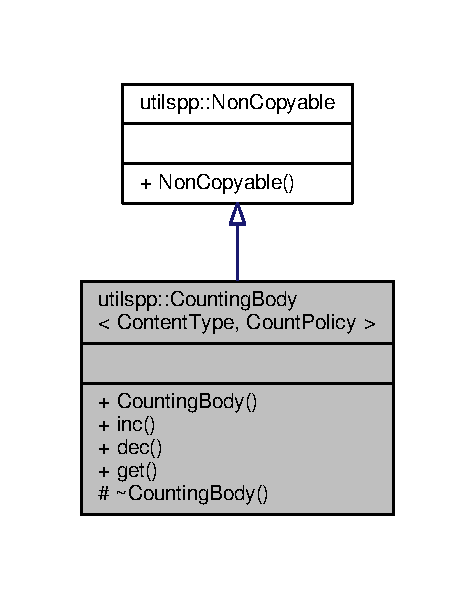
\includegraphics[width=228pt]{classutilspp_1_1CountingBody__inherit__graph}
\end{center}
\end{figure}


Collaboration diagram for utilspp\-:\-:Counting\-Body$<$ Content\-Type, Count\-Policy $>$\-:
\nopagebreak
\begin{figure}[H]
\begin{center}
\leavevmode
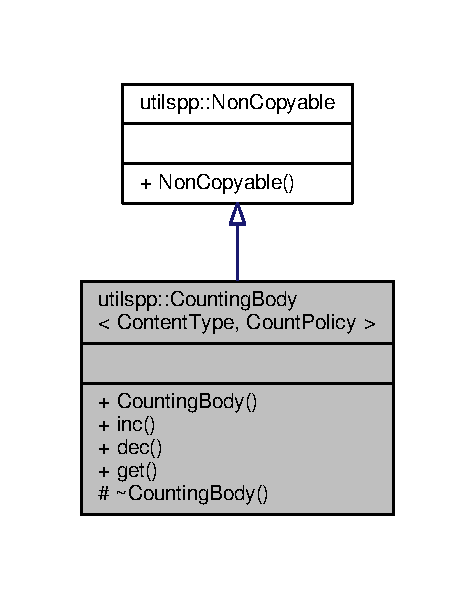
\includegraphics[width=228pt]{classutilspp_1_1CountingBody__coll__graph}
\end{center}
\end{figure}
\subsection*{Public Member Functions}
\begin{DoxyCompactItemize}
\item 
\hypertarget{classutilspp_1_1CountingBody_a1cdd0127a4df9faacebcf6e6485a17d0}{{\bfseries Counting\-Body} (Content\-Type $\ast$body)}\label{classutilspp_1_1CountingBody_a1cdd0127a4df9faacebcf6e6485a17d0}

\item 
\hypertarget{classutilspp_1_1CountingBody_ab614dec16baa509684b7ff64d8f1ab0e}{void {\bfseries inc} ()}\label{classutilspp_1_1CountingBody_ab614dec16baa509684b7ff64d8f1ab0e}

\item 
\hypertarget{classutilspp_1_1CountingBody_a9a5eee9f042935a08b526c4dd4191b74}{void {\bfseries dec} ()}\label{classutilspp_1_1CountingBody_a9a5eee9f042935a08b526c4dd4191b74}

\item 
\hypertarget{classutilspp_1_1CountingBody_ae6305c6f6e5765cecb318c2047994ab5}{Content\-Type $\ast$ {\bfseries get} ()}\label{classutilspp_1_1CountingBody_ae6305c6f6e5765cecb318c2047994ab5}

\end{DoxyCompactItemize}


The documentation for this class was generated from the following file\-:\begin{DoxyCompactItemize}
\item 
include/utilspp/Smart\-Ptr.\-hpp\end{DoxyCompactItemize}

\hypertarget{classutilspp_1_1CreationStatic}{\section{utilspp\-:\-:Creation\-Static$<$ T $>$ Class Template Reference}
\label{classutilspp_1_1CreationStatic}\index{utilspp\-::\-Creation\-Static$<$ T $>$@{utilspp\-::\-Creation\-Static$<$ T $>$}}
}


Collaboration diagram for utilspp\-:\-:Creation\-Static$<$ T $>$\-:
\nopagebreak
\begin{figure}[H]
\begin{center}
\leavevmode
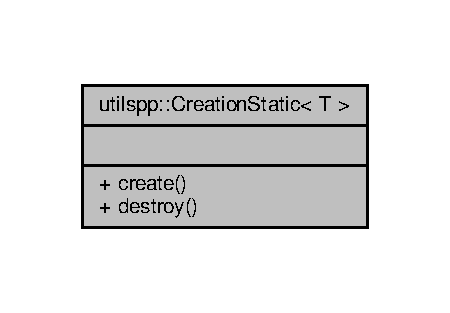
\includegraphics[width=216pt]{classutilspp_1_1CreationStatic__coll__graph}
\end{center}
\end{figure}
\subsection*{Static Public Member Functions}
\begin{DoxyCompactItemize}
\item 
\hypertarget{classutilspp_1_1CreationStatic_adf936d61ce6ba3f6310dc02fc368ccc9}{static T $\ast$ {\bfseries create} ()}\label{classutilspp_1_1CreationStatic_adf936d61ce6ba3f6310dc02fc368ccc9}

\item 
\hypertarget{classutilspp_1_1CreationStatic_a3470e96e86e9f7eb24d591f170645b1c}{static void {\bfseries destroy} (T $\ast$obj)}\label{classutilspp_1_1CreationStatic_a3470e96e86e9f7eb24d591f170645b1c}

\end{DoxyCompactItemize}


The documentation for this class was generated from the following files\-:\begin{DoxyCompactItemize}
\item 
include/utilspp/singleton/Creation\-Static.\-hpp\item 
include/utilspp/singleton/Creation\-Static.\-inl\end{DoxyCompactItemize}

\hypertarget{structutilspp_1_1CreationUsingNew}{\section{utilspp\-:\-:Creation\-Using\-New$<$ T $>$ Struct Template Reference}
\label{structutilspp_1_1CreationUsingNew}\index{utilspp\-::\-Creation\-Using\-New$<$ T $>$@{utilspp\-::\-Creation\-Using\-New$<$ T $>$}}
}


Collaboration diagram for utilspp\-:\-:Creation\-Using\-New$<$ T $>$\-:
\nopagebreak
\begin{figure}[H]
\begin{center}
\leavevmode
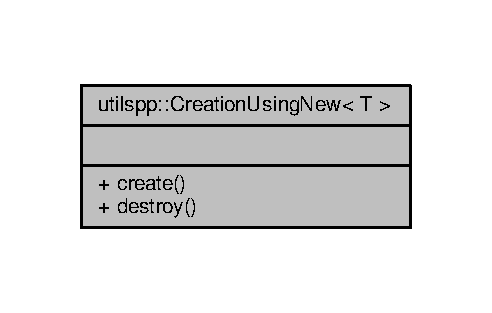
\includegraphics[width=236pt]{structutilspp_1_1CreationUsingNew__coll__graph}
\end{center}
\end{figure}
\subsection*{Static Public Member Functions}
\begin{DoxyCompactItemize}
\item 
\hypertarget{structutilspp_1_1CreationUsingNew_a105f82c90ac834842f9a8d8f7e9890fd}{static T $\ast$ {\bfseries create} ()}\label{structutilspp_1_1CreationUsingNew_a105f82c90ac834842f9a8d8f7e9890fd}

\item 
\hypertarget{structutilspp_1_1CreationUsingNew_a808b9cb86569dcef4fa7d13bf0fbbea8}{static void {\bfseries destroy} (T $\ast$obj)}\label{structutilspp_1_1CreationUsingNew_a808b9cb86569dcef4fa7d13bf0fbbea8}

\end{DoxyCompactItemize}


The documentation for this struct was generated from the following files\-:\begin{DoxyCompactItemize}
\item 
include/utilspp/singleton/Creation\-Using\-New.\-hpp\item 
include/utilspp/singleton/Creation\-Using\-New.\-inl\end{DoxyCompactItemize}

\hypertarget{classCurlCommunicator}{\section{Curl\-Communicator Class Reference}
\label{classCurlCommunicator}\index{Curl\-Communicator@{Curl\-Communicator}}
}


Class for communication This class provides the communication for downloading job files or uploading log files.  




{\ttfamily \#include $<$Curl\-Communicator.\-hpp$>$}



Collaboration diagram for Curl\-Communicator\-:\nopagebreak
\begin{figure}[H]
\begin{center}
\leavevmode
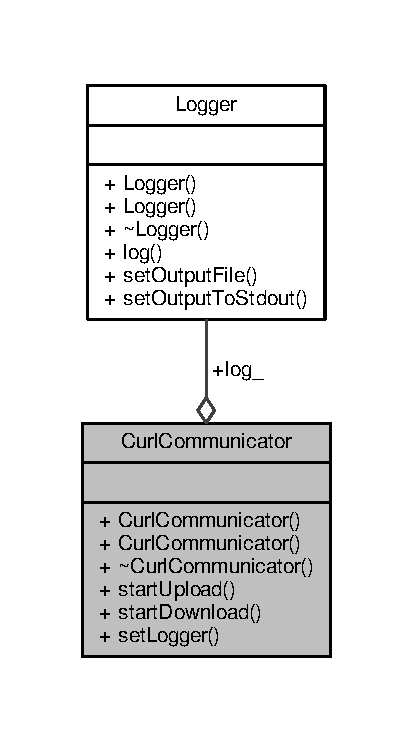
\includegraphics[width=198pt]{classCurlCommunicator__coll__graph}
\end{center}
\end{figure}
\subsection*{Public Member Functions}
\begin{DoxyCompactItemize}
\item 
\hypertarget{classCurlCommunicator_a67f50f315cc1e99042637aa67dd14c03}{\hyperlink{classCurlCommunicator_a67f50f315cc1e99042637aa67dd14c03}{Curl\-Communicator} ()}\label{classCurlCommunicator_a67f50f315cc1e99042637aa67dd14c03}

\begin{DoxyCompactList}\small\item\em Ctor. \end{DoxyCompactList}\item 
\hyperlink{classCurlCommunicator_a54f8093da6f396f88015f000f96e537a}{Curl\-Communicator} (string user, string pw, int time\-Out\-Sec, int retries)
\begin{DoxyCompactList}\small\item\em Ctor. \end{DoxyCompactList}\item 
\hypertarget{classCurlCommunicator_ae6280940aaed63c9d8d4da2a930eb719}{\hyperlink{classCurlCommunicator_ae6280940aaed63c9d8d4da2a930eb719}{$\sim$\-Curl\-Communicator} ()}\label{classCurlCommunicator_ae6280940aaed63c9d8d4da2a930eb719}

\begin{DoxyCompactList}\small\item\em Dtor. \end{DoxyCompactList}\item 
int \hyperlink{classCurlCommunicator_a33dd04c8d5075d13cba92090f8482211}{start\-Upload} (string url, string save\-Filename)
\begin{DoxyCompactList}\small\item\em Upload a given file to the given url. \end{DoxyCompactList}\item 
int \hyperlink{classCurlCommunicator_a02e733609c88dbf00811b3d61d83abae}{start\-Download} (string url, string save\-Filename)
\begin{DoxyCompactList}\small\item\em Downloads a requested file from the given url. \end{DoxyCompactList}\end{DoxyCompactItemize}
\subsection*{Static Public Member Functions}
\begin{DoxyCompactItemize}
\item 
static void \hyperlink{classCurlCommunicator_a006af85c4b542cad443f5f96414e4765}{set\-Logger} (\hyperlink{classLogger}{Logger} \&log)
\begin{DoxyCompactList}\small\item\em Setter for logger. \end{DoxyCompactList}\end{DoxyCompactItemize}
\subsection*{Static Public Attributes}
\begin{DoxyCompactItemize}
\item 
\hypertarget{classCurlCommunicator_a549e31b1922eb221203619dc2c0d5c4e}{static \hyperlink{classLogger}{Logger} \hyperlink{classCurlCommunicator_a549e31b1922eb221203619dc2c0d5c4e}{log\-\_\-} = \hyperlink{classLogger}{Logger}()}\label{classCurlCommunicator_a549e31b1922eb221203619dc2c0d5c4e}

\begin{DoxyCompactList}\small\item\em \hyperlink{classLogger}{Logger} for tracking and generating report to upload. \end{DoxyCompactList}\end{DoxyCompactItemize}


\subsection{Detailed Description}
Class for communication This class provides the communication for downloading job files or uploading log files. 

To communicate with the server the curl libary is used 

\subsection{Constructor \& Destructor Documentation}
\hypertarget{classCurlCommunicator_a54f8093da6f396f88015f000f96e537a}{\index{Curl\-Communicator@{Curl\-Communicator}!Curl\-Communicator@{Curl\-Communicator}}
\index{Curl\-Communicator@{Curl\-Communicator}!CurlCommunicator@{Curl\-Communicator}}
\subsubsection[{Curl\-Communicator}]{\setlength{\rightskip}{0pt plus 5cm}Curl\-Communicator\-::\-Curl\-Communicator (
\begin{DoxyParamCaption}
\item[{string}]{user, }
\item[{string}]{pw, }
\item[{int}]{time\-Out\-Sec, }
\item[{int}]{retries}
\end{DoxyParamCaption}
)}}\label{classCurlCommunicator_a54f8093da6f396f88015f000f96e537a}


Ctor. 


\begin{DoxyParams}{Parameters}
{\em string} & with user name \\
\hline
{\em string} & with password \\
\hline
{\em int} & with time for connection timeout in seconds \\
\hline
{\em int} & with amount of retries to make before say connection falied \\
\hline
\end{DoxyParams}


\subsection{Member Function Documentation}
\hypertarget{classCurlCommunicator_a006af85c4b542cad443f5f96414e4765}{\index{Curl\-Communicator@{Curl\-Communicator}!set\-Logger@{set\-Logger}}
\index{set\-Logger@{set\-Logger}!CurlCommunicator@{Curl\-Communicator}}
\subsubsection[{set\-Logger}]{\setlength{\rightskip}{0pt plus 5cm}static void Curl\-Communicator\-::set\-Logger (
\begin{DoxyParamCaption}
\item[{{\bf Logger} \&}]{log}
\end{DoxyParamCaption}
)\hspace{0.3cm}{\ttfamily [inline]}, {\ttfamily [static]}}}\label{classCurlCommunicator_a006af85c4b542cad443f5f96414e4765}


Setter for logger. 


\begin{DoxyParams}{Parameters}
{\em \hyperlink{classLogger}{Logger}} & \\
\hline
\end{DoxyParams}
\hypertarget{classCurlCommunicator_a02e733609c88dbf00811b3d61d83abae}{\index{Curl\-Communicator@{Curl\-Communicator}!start\-Download@{start\-Download}}
\index{start\-Download@{start\-Download}!CurlCommunicator@{Curl\-Communicator}}
\subsubsection[{start\-Download}]{\setlength{\rightskip}{0pt plus 5cm}int Curl\-Communicator\-::start\-Download (
\begin{DoxyParamCaption}
\item[{string}]{url, }
\item[{string}]{save\-Filename}
\end{DoxyParamCaption}
)}}\label{classCurlCommunicator_a02e733609c88dbf00811b3d61d83abae}


Downloads a requested file from the given url. 


\begin{DoxyParams}{Parameters}
{\em string} & with url \\
\hline
{\em string} & with file to download to \\
\hline
\end{DoxyParams}
\begin{DoxyReturn}{Returns}
int with succsess 1 or fail 0 
\end{DoxyReturn}
\hypertarget{classCurlCommunicator_a33dd04c8d5075d13cba92090f8482211}{\index{Curl\-Communicator@{Curl\-Communicator}!start\-Upload@{start\-Upload}}
\index{start\-Upload@{start\-Upload}!CurlCommunicator@{Curl\-Communicator}}
\subsubsection[{start\-Upload}]{\setlength{\rightskip}{0pt plus 5cm}int Curl\-Communicator\-::start\-Upload (
\begin{DoxyParamCaption}
\item[{string}]{url, }
\item[{string}]{save\-Filename}
\end{DoxyParamCaption}
)}}\label{classCurlCommunicator_a33dd04c8d5075d13cba92090f8482211}


Upload a given file to the given url. 


\begin{DoxyParams}{Parameters}
{\em string} & with url \\
\hline
{\em string} & with file to upload \\
\hline
\end{DoxyParams}
\begin{DoxyReturn}{Returns}
int with succsess 1 or fail 0 
\end{DoxyReturn}


The documentation for this class was generated from the following files\-:\begin{DoxyCompactItemize}
\item 
include/\hyperlink{CurlCommunicator_8hpp}{Curl\-Communicator.\-hpp}\item 
src/Curl\-Communicator.\-cpp\end{DoxyCompactItemize}

\hypertarget{classcurlpp_1_1internal_1_1CurlHandle}{\section{curlpp\-:\-:internal\-:\-:Curl\-Handle Class Reference}
\label{classcurlpp_1_1internal_1_1CurlHandle}\index{curlpp\-::internal\-::\-Curl\-Handle@{curlpp\-::internal\-::\-Curl\-Handle}}
}


Wrapper for C\-U\-R\-L $\ast$ handle.  




{\ttfamily \#include $<$Curl\-Handle.\-hpp$>$}



Collaboration diagram for curlpp\-:\-:internal\-:\-:Curl\-Handle\-:
\nopagebreak
\begin{figure}[H]
\begin{center}
\leavevmode
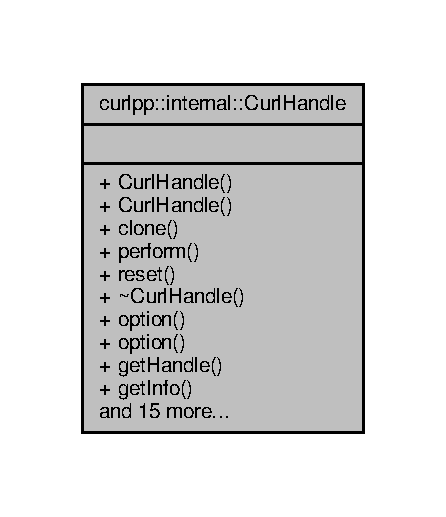
\includegraphics[width=214pt]{classcurlpp_1_1internal_1_1CurlHandle__coll__graph}
\end{center}
\end{figure}
\subsection*{Public Member Functions}
\begin{DoxyCompactItemize}
\item 
\hypertarget{classcurlpp_1_1internal_1_1CurlHandle_adb6fcf013135805a31c3dc065d0e61e7}{{\bfseries Curl\-Handle} (C\-U\-R\-L $\ast$handle)}\label{classcurlpp_1_1internal_1_1CurlHandle_adb6fcf013135805a31c3dc065d0e61e7}

\item 
\hypertarget{classcurlpp_1_1internal_1_1CurlHandle_a580b97234e3973eaa783272c2e12cded}{std\-::auto\-\_\-ptr$<$ \hyperlink{classcurlpp_1_1internal_1_1CurlHandle}{Curl\-Handle} $>$ {\bfseries clone} () const }\label{classcurlpp_1_1internal_1_1CurlHandle_a580b97234e3973eaa783272c2e12cded}

\item 
\hypertarget{classcurlpp_1_1internal_1_1CurlHandle_a9b2fa00ec86b7c6ea86068eed1ae4b71}{void \hyperlink{classcurlpp_1_1internal_1_1CurlHandle_a9b2fa00ec86b7c6ea86068eed1ae4b71}{perform} ()}\label{classcurlpp_1_1internal_1_1CurlHandle_a9b2fa00ec86b7c6ea86068eed1ae4b71}

\begin{DoxyCompactList}\small\item\em Calls curl\-\_\-easy\-\_\-perform on the handle and throws exceptions on errors. \end{DoxyCompactList}\item 
\hypertarget{classcurlpp_1_1internal_1_1CurlHandle_ac884758256b2735eb2ab1f037c38ce9f}{void \hyperlink{classcurlpp_1_1internal_1_1CurlHandle_ac884758256b2735eb2ab1f037c38ce9f}{reset} ()}\label{classcurlpp_1_1internal_1_1CurlHandle_ac884758256b2735eb2ab1f037c38ce9f}

\begin{DoxyCompactList}\small\item\em Simply calls curl\-\_\-easy\-\_\-reset on the handle. \end{DoxyCompactList}\item 
\hypertarget{classcurlpp_1_1internal_1_1CurlHandle_a715e437b50f34871318e8256d7c78765}{{\footnotesize template$<$typename Option\-Type $>$ }\\void \hyperlink{classcurlpp_1_1internal_1_1CurlHandle_a715e437b50f34871318e8256d7c78765}{option} (C\-U\-R\-Loption option, Option\-Type value)}\label{classcurlpp_1_1internal_1_1CurlHandle_a715e437b50f34871318e8256d7c78765}

\begin{DoxyCompactList}\small\item\em Calls curl\-\_\-easy\-\_\-setopt on the option. \end{DoxyCompactList}\item 
\hypertarget{classcurlpp_1_1internal_1_1CurlHandle_af7cf67e4dfc41b2da23a6005b0f396d3}{{\footnotesize template$<$typename Option\-Type , C\-U\-R\-Loption option\-Type$>$ }\\void \hyperlink{classcurlpp_1_1internal_1_1CurlHandle_af7cf67e4dfc41b2da23a6005b0f396d3}{option} (Option\-Type value)}\label{classcurlpp_1_1internal_1_1CurlHandle_af7cf67e4dfc41b2da23a6005b0f396d3}

\begin{DoxyCompactList}\small\item\em Calls curl\-\_\-easy\-\_\-setopt on the option. \end{DoxyCompactList}\item 
C\-U\-R\-L $\ast$ \hyperlink{classcurlpp_1_1internal_1_1CurlHandle_a219dded6f057d576ec1a1eb76061e0c0}{get\-Handle} () const 
\begin{DoxyCompactList}\small\item\em This function will return the C\-U\-R\-L $\ast$ handle. \end{DoxyCompactList}\item 
{\footnotesize template$<$typename T $>$ }\\void \hyperlink{classcurlpp_1_1internal_1_1CurlHandle_ad217ec54215cf880b474a1e1249b5f4e}{get\-Info} (C\-U\-R\-L\-I\-N\-F\-O info, T \&value) const 
\begin{DoxyCompactList}\small\item\em Request internal information from the curl session with this function. \end{DoxyCompactList}\item 
\hypertarget{classcurlpp_1_1internal_1_1CurlHandle_ab4a680ad19c629823ed6baed2582f1b7}{{\footnotesize template$<$typename Functor\-Type $>$ }\\Functor\-Type\-::\-Result\-Type {\bfseries execute} (Functor\-Type functor, typename Functor\-Type\-::\-Param\-List params)}\label{classcurlpp_1_1internal_1_1CurlHandle_ab4a680ad19c629823ed6baed2582f1b7}

\item 
\hypertarget{classcurlpp_1_1internal_1_1CurlHandle_ac62f315ca3a5150786a06914b1858daa}{size\-\_\-t {\bfseries execute\-Write\-Functor} (char $\ast$buffer, size\-\_\-t size, size\-\_\-t nitems)}\label{classcurlpp_1_1internal_1_1CurlHandle_ac62f315ca3a5150786a06914b1858daa}

\item 
\hypertarget{classcurlpp_1_1internal_1_1CurlHandle_a848df273cfbb8cae7413a0e160707f37}{void {\bfseries set\-Write\-Functor} (\hyperlink{classutilspp_1_1Functor}{curlpp\-::types\-::\-Write\-Function\-Functor} functor)}\label{classcurlpp_1_1internal_1_1CurlHandle_a848df273cfbb8cae7413a0e160707f37}

\item 
\hypertarget{classcurlpp_1_1internal_1_1CurlHandle_ac7662650f40ad7fdb6fc8e95ff979fa9}{size\-\_\-t {\bfseries execute\-Header\-Functor} (char $\ast$buffer, size\-\_\-t size, size\-\_\-t nitems)}\label{classcurlpp_1_1internal_1_1CurlHandle_ac7662650f40ad7fdb6fc8e95ff979fa9}

\item 
\hypertarget{classcurlpp_1_1internal_1_1CurlHandle_a585ae1e9991534e48d073f56361ec5ff}{void {\bfseries set\-Header\-Functor} (\hyperlink{classutilspp_1_1Functor}{curlpp\-::types\-::\-Write\-Function\-Functor} functor)}\label{classcurlpp_1_1internal_1_1CurlHandle_a585ae1e9991534e48d073f56361ec5ff}

\item 
\hypertarget{classcurlpp_1_1internal_1_1CurlHandle_a34a51c2a15f08b9643025801184738eb}{size\-\_\-t {\bfseries execute\-Read\-Functor} (char $\ast$buffer, size\-\_\-t size, size\-\_\-t nitems)}\label{classcurlpp_1_1internal_1_1CurlHandle_a34a51c2a15f08b9643025801184738eb}

\item 
\hypertarget{classcurlpp_1_1internal_1_1CurlHandle_ae116674f2a89956247d5cf85737d47de}{void {\bfseries set\-Read\-Functor} (\hyperlink{classutilspp_1_1Functor}{curlpp\-::types\-::\-Read\-Function\-Functor} functor)}\label{classcurlpp_1_1internal_1_1CurlHandle_ae116674f2a89956247d5cf85737d47de}

\item 
\hypertarget{classcurlpp_1_1internal_1_1CurlHandle_a86621767b2fbb1343ceac9dbe3b2a07b}{int {\bfseries execute\-Progress\-Functor} (double dltotal, double dlnow, double ultotal, double ulnow)}\label{classcurlpp_1_1internal_1_1CurlHandle_a86621767b2fbb1343ceac9dbe3b2a07b}

\item 
\hypertarget{classcurlpp_1_1internal_1_1CurlHandle_abda84c7e8f6e1d92de16027f2e30fdcd}{void {\bfseries set\-Progress\-Functor} (\hyperlink{classutilspp_1_1Functor}{curlpp\-::types\-::\-Progress\-Function\-Functor} functor)}\label{classcurlpp_1_1internal_1_1CurlHandle_abda84c7e8f6e1d92de16027f2e30fdcd}

\item 
\hypertarget{classcurlpp_1_1internal_1_1CurlHandle_a1de5d35d03a2400e21bfd5b3e4f331e6}{int {\bfseries execute\-Debug\-Functor} (curl\-\_\-infotype, char $\ast$, size\-\_\-t)}\label{classcurlpp_1_1internal_1_1CurlHandle_a1de5d35d03a2400e21bfd5b3e4f331e6}

\item 
\hypertarget{classcurlpp_1_1internal_1_1CurlHandle_abe1061232803c541f99c446d8d6a1edd}{void {\bfseries set\-Debug\-Functor} (\hyperlink{classutilspp_1_1Functor}{curlpp\-::types\-::\-Debug\-Function\-Functor} functor)}\label{classcurlpp_1_1internal_1_1CurlHandle_abe1061232803c541f99c446d8d6a1edd}

\item 
\hypertarget{classcurlpp_1_1internal_1_1CurlHandle_a8e3ef0099fd8dd1d0c4c342479fa5edc}{C\-U\-R\-Lcode {\bfseries execute\-Ssl\-Ctx\-Functor} (void $\ast$ssl\-\_\-ctx)}\label{classcurlpp_1_1internal_1_1CurlHandle_a8e3ef0099fd8dd1d0c4c342479fa5edc}

\item 
\hypertarget{classcurlpp_1_1internal_1_1CurlHandle_a01ff1b85447df61c5cf01ce969b1f86a}{void {\bfseries set\-Ssl\-Ctx\-Functor} (\hyperlink{classutilspp_1_1Functor}{curlpp\-::types\-::\-Ssl\-Ctx\-Function\-Functor} functor)}\label{classcurlpp_1_1internal_1_1CurlHandle_a01ff1b85447df61c5cf01ce969b1f86a}

\item 
\hypertarget{classcurlpp_1_1internal_1_1CurlHandle_ac84ef815b10c99f21e48b59988e9801c}{void {\bfseries set\-Exception} (\hyperlink{classcurlpp_1_1CallbackExceptionBase}{curlpp\-::\-Callback\-Exception\-Base} $\ast$e)}\label{classcurlpp_1_1internal_1_1CurlHandle_ac84ef815b10c99f21e48b59988e9801c}

\item 
\hypertarget{classcurlpp_1_1internal_1_1CurlHandle_af75c10e8106f51806e7347a51d8824c8}{void {\bfseries throw\-Exception} ()}\label{classcurlpp_1_1internal_1_1CurlHandle_af75c10e8106f51806e7347a51d8824c8}

\end{DoxyCompactItemize}


\subsection{Detailed Description}
Wrapper for C\-U\-R\-L $\ast$ handle. 

\subsection{Member Function Documentation}
\hypertarget{classcurlpp_1_1internal_1_1CurlHandle_a219dded6f057d576ec1a1eb76061e0c0}{\index{curlpp\-::internal\-::\-Curl\-Handle@{curlpp\-::internal\-::\-Curl\-Handle}!get\-Handle@{get\-Handle}}
\index{get\-Handle@{get\-Handle}!curlpp::internal::CurlHandle@{curlpp\-::internal\-::\-Curl\-Handle}}
\subsubsection[{get\-Handle}]{\setlength{\rightskip}{0pt plus 5cm}C\-U\-R\-L $\ast$ curlpp\-::internal\-::\-Curl\-Handle\-::get\-Handle (
\begin{DoxyParamCaption}
{}
\end{DoxyParamCaption}
) const}}\label{classcurlpp_1_1internal_1_1CurlHandle_a219dded6f057d576ec1a1eb76061e0c0}


This function will return the C\-U\-R\-L $\ast$ handle. 

D\-O N\-O\-T use this, unless you R\-E\-A\-L\-L\-Y know what you are doing. \hypertarget{classcurlpp_1_1internal_1_1CurlHandle_ad217ec54215cf880b474a1e1249b5f4e}{\index{curlpp\-::internal\-::\-Curl\-Handle@{curlpp\-::internal\-::\-Curl\-Handle}!get\-Info@{get\-Info}}
\index{get\-Info@{get\-Info}!curlpp::internal::CurlHandle@{curlpp\-::internal\-::\-Curl\-Handle}}
\subsubsection[{get\-Info}]{\setlength{\rightskip}{0pt plus 5cm}template$<$typename T $>$ void curlpp\-::internal\-::\-Curl\-Handle\-::get\-Info (
\begin{DoxyParamCaption}
\item[{C\-U\-R\-L\-I\-N\-F\-O}]{info, }
\item[{T \&}]{value}
\end{DoxyParamCaption}
) const}}\label{classcurlpp_1_1internal_1_1CurlHandle_ad217ec54215cf880b474a1e1249b5f4e}


Request internal information from the curl session with this function. 

The third argument M\-U\-S\-T be a pointer to a long, a pointer to a char $\ast$, a pointer to a struct curl\-\_\-slist $\ast$ or a pointer to a double. 

The documentation for this class was generated from the following files\-:\begin{DoxyCompactItemize}
\item 
include/curlpp/internal/Curl\-Handle.\-hpp\item 
include/curlpp/internal/Curl\-Handle.\-inl\item 
src/curlpp/internal/Curl\-Handle.\-cpp\end{DoxyCompactItemize}

\hypertarget{structutilspp_1_1PrivateMembers_1_1Deleter}{\section{utilspp\-:\-:Private\-Members\-:\-:Deleter$<$ T $>$ Struct Template Reference}
\label{structutilspp_1_1PrivateMembers_1_1Deleter}\index{utilspp\-::\-Private\-Members\-::\-Deleter$<$ T $>$@{utilspp\-::\-Private\-Members\-::\-Deleter$<$ T $>$}}
}


Helper class for Destroyer.  




{\ttfamily \#include $<$Private\-Members.\-hpp$>$}



Collaboration diagram for utilspp\-:\-:Private\-Members\-:\-:Deleter$<$ T $>$\-:
\nopagebreak
\begin{figure}[H]
\begin{center}
\leavevmode
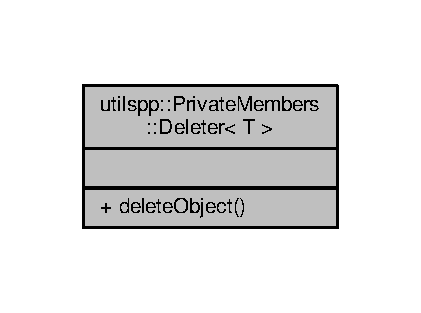
\includegraphics[width=202pt]{structutilspp_1_1PrivateMembers_1_1Deleter__coll__graph}
\end{center}
\end{figure}
\subsection*{Public Member Functions}
\begin{DoxyCompactItemize}
\item 
\hypertarget{structutilspp_1_1PrivateMembers_1_1Deleter_ac1733f7f90b94aaba61df48476bfba4a}{void {\bfseries delete\-Object} (T $\ast$obj)}\label{structutilspp_1_1PrivateMembers_1_1Deleter_ac1733f7f90b94aaba61df48476bfba4a}

\end{DoxyCompactItemize}


\subsection{Detailed Description}
\subsubsection*{template$<$typename T$>$struct utilspp\-::\-Private\-Members\-::\-Deleter$<$ T $>$}

Helper class for Destroyer. 

The documentation for this struct was generated from the following files\-:\begin{DoxyCompactItemize}
\item 
include/utilspp/singleton/Private\-Members.\-hpp\item 
include/utilspp/singleton/Private\-Members.\-inl\end{DoxyCompactItemize}

\hypertarget{classcurlpp_1_1Easy}{\section{curlpp\-:\-:Easy Class Reference}
\label{classcurlpp_1_1Easy}\index{curlpp\-::\-Easy@{curlpp\-::\-Easy}}
}


\hyperlink{classcurlpp_1_1Easy}{Easy} class.  




{\ttfamily \#include $<$Easy.\-hpp$>$}



Collaboration diagram for curlpp\-:\-:Easy\-:
\nopagebreak
\begin{figure}[H]
\begin{center}
\leavevmode
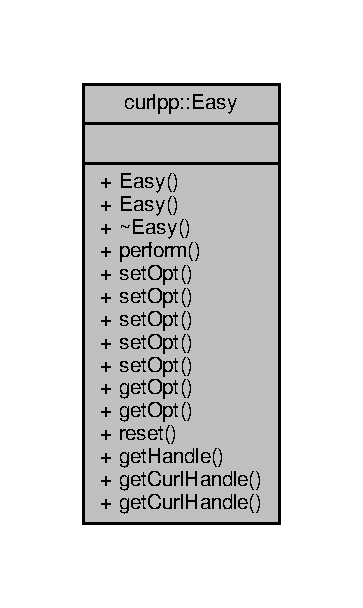
\includegraphics[width=174pt]{classcurlpp_1_1Easy__coll__graph}
\end{center}
\end{figure}
\subsection*{Public Member Functions}
\begin{DoxyCompactItemize}
\item 
\hypertarget{classcurlpp_1_1Easy_a8c39568bc33b367d89337e216dc53acf}{\hyperlink{classcurlpp_1_1Easy_a8c39568bc33b367d89337e216dc53acf}{Easy} (std\-::auto\-\_\-ptr$<$ \hyperlink{classcurlpp_1_1internal_1_1CurlHandle}{internal\-::\-Curl\-Handle} $>$ handle)}\label{classcurlpp_1_1Easy_a8c39568bc33b367d89337e216dc53acf}

\begin{DoxyCompactList}\small\item\em This allow to have a handle, which might have some option set, but we don't care about them. \end{DoxyCompactList}\item 
\hypertarget{classcurlpp_1_1Easy_a3f6b472981811111365dbc537b06218d}{void \hyperlink{classcurlpp_1_1Easy_a3f6b472981811111365dbc537b06218d}{perform} ()}\label{classcurlpp_1_1Easy_a3f6b472981811111365dbc537b06218d}

\begin{DoxyCompactList}\small\item\em it will call the curl\-\_\-easy\-\_\-perform function will all the options previously set for this handle. \end{DoxyCompactList}\item 
\hypertarget{classcurlpp_1_1Easy_ae5b79592f7f01fab768f0dd733188e3b}{virtual void \hyperlink{classcurlpp_1_1Easy_ae5b79592f7f01fab768f0dd733188e3b}{set\-Opt} (const \hyperlink{classcurlpp_1_1OptionBase}{Option\-Base} \&option)}\label{classcurlpp_1_1Easy_ae5b79592f7f01fab768f0dd733188e3b}

\begin{DoxyCompactList}\small\item\em This function will set the option value of the \hyperlink{classcurlpp_1_1OptionBase}{Option\-Base} to the handle. \end{DoxyCompactList}\item 
\hypertarget{classcurlpp_1_1Easy_a576f15e11c3d691f389bffafab420f63}{virtual void \hyperlink{classcurlpp_1_1Easy_a576f15e11c3d691f389bffafab420f63}{set\-Opt} (std\-::auto\-\_\-ptr$<$ \hyperlink{classcurlpp_1_1OptionBase}{Option\-Base} $>$ option)}\label{classcurlpp_1_1Easy_a576f15e11c3d691f389bffafab420f63}

\begin{DoxyCompactList}\small\item\em This function will set the option value of the \hyperlink{classcurlpp_1_1OptionBase}{Option\-Base} to the handle. \end{DoxyCompactList}\item 
virtual void \hyperlink{classcurlpp_1_1Easy_a64b45db88ad188cf25398b4ead5f13a5}{set\-Opt} (\hyperlink{classcurlpp_1_1OptionBase}{Option\-Base} $\ast$option)
\begin{DoxyCompactList}\small\item\em This function will set the option value of the \hyperlink{classcurlpp_1_1OptionBase}{Option\-Base} to the handle. \end{DoxyCompactList}\item 
\hypertarget{classcurlpp_1_1Easy_aa3b2f0c550d270403be29ad05f93e3b0}{{\footnotesize template$<$typename Option\-Trait $>$ }\\void \hyperlink{classcurlpp_1_1Easy_aa3b2f0c550d270403be29ad05f93e3b0}{set\-Opt} (typename Option\-Trait\-::\-Param\-Type)}\label{classcurlpp_1_1Easy_aa3b2f0c550d270403be29ad05f93e3b0}

\begin{DoxyCompactList}\small\item\em This function will create \hyperlink{classcurlpp_1_1OptionTrait}{Option\-Trait} class with the value given and call virtual void \hyperlink{classcurlpp_1_1Easy_ae5b79592f7f01fab768f0dd733188e3b}{set\-Opt(const Option\-Base \& option)} with it. \end{DoxyCompactList}\item 
\hypertarget{classcurlpp_1_1Easy_a627196122ee249d379302bc86b569e9b}{{\footnotesize template$<$typename Input\-Iterator $>$ }\\void \hyperlink{classcurlpp_1_1Easy_a627196122ee249d379302bc86b569e9b}{set\-Opt} (Input\-Iterator first, Input\-Iterator last)}\label{classcurlpp_1_1Easy_a627196122ee249d379302bc86b569e9b}

\begin{DoxyCompactList}\small\item\em Setting options from custom container with curlpp options. \end{DoxyCompactList}\item 
void \hyperlink{classcurlpp_1_1Easy_afb31f0536e0767f0016ed04fdb935b21}{get\-Opt} (\hyperlink{classcurlpp_1_1OptionBase}{Option\-Base} $\ast$option) const 
\begin{DoxyCompactList}\small\item\em This function will get the current option value of the corresponding \hyperlink{classcurlpp_1_1OptionBase}{Option\-Base}. \end{DoxyCompactList}\item 
void \hyperlink{classcurlpp_1_1Easy_a9103b1438874709c1ec42f430173edaf}{get\-Opt} (\hyperlink{classcurlpp_1_1OptionBase}{Option\-Base} \&option) const 
\begin{DoxyCompactList}\small\item\em This function will get the current option value of the corresponding \hyperlink{classcurlpp_1_1OptionBase}{Option\-Base}. \end{DoxyCompactList}\item 
\hypertarget{classcurlpp_1_1Easy_a2e9dcb9179225771a28e6acda748b750}{virtual void \hyperlink{classcurlpp_1_1Easy_a2e9dcb9179225771a28e6acda748b750}{reset} ()}\label{classcurlpp_1_1Easy_a2e9dcb9179225771a28e6acda748b750}

\begin{DoxyCompactList}\small\item\em Get all options. \end{DoxyCompactList}\item 
C\-U\-R\-L $\ast$ \hyperlink{classcurlpp_1_1Easy_af40b3ee39a944a728599176e9dece30e}{get\-Handle} () const 
\begin{DoxyCompactList}\small\item\em This function will return the c\-U\-R\-L $\ast$ handle. \end{DoxyCompactList}\item 
\hypertarget{classcurlpp_1_1Easy_acf38b0fd04b0b02fded31849f87bea43}{\hyperlink{classcurlpp_1_1internal_1_1CurlHandle}{internal\-::\-Curl\-Handle} \& {\bfseries get\-Curl\-Handle} ()}\label{classcurlpp_1_1Easy_acf38b0fd04b0b02fded31849f87bea43}

\item 
\hypertarget{classcurlpp_1_1Easy_a49fbfde3465fdd5f51a89f3e012fa6bb}{const \hyperlink{classcurlpp_1_1internal_1_1CurlHandle}{internal\-::\-Curl\-Handle} \& {\bfseries get\-Curl\-Handle} () const }\label{classcurlpp_1_1Easy_a49fbfde3465fdd5f51a89f3e012fa6bb}

\end{DoxyCompactItemize}
\subsection*{Friends}
\begin{DoxyCompactItemize}
\item 
\hypertarget{classcurlpp_1_1Easy_ae5b89291153dc90fe7e0204270d0c5af}{struct {\bfseries Info\-Getter}}\label{classcurlpp_1_1Easy_ae5b89291153dc90fe7e0204270d0c5af}

\end{DoxyCompactItemize}


\subsection{Detailed Description}
\hyperlink{classcurlpp_1_1Easy}{Easy} class. 

Detailed description. 

\subsection{Member Function Documentation}
\hypertarget{classcurlpp_1_1Easy_af40b3ee39a944a728599176e9dece30e}{\index{curlpp\-::\-Easy@{curlpp\-::\-Easy}!get\-Handle@{get\-Handle}}
\index{get\-Handle@{get\-Handle}!curlpp::Easy@{curlpp\-::\-Easy}}
\subsubsection[{get\-Handle}]{\setlength{\rightskip}{0pt plus 5cm}C\-U\-R\-L $\ast$ curlpp\-::\-Easy\-::get\-Handle (
\begin{DoxyParamCaption}
{}
\end{DoxyParamCaption}
) const}}\label{classcurlpp_1_1Easy_af40b3ee39a944a728599176e9dece30e}


This function will return the c\-U\-R\-L $\ast$ handle. 

D\-O N\-O\-T use this, unless you R\-E\-A\-L\-L\-Y know what you are doing. \hypertarget{classcurlpp_1_1Easy_afb31f0536e0767f0016ed04fdb935b21}{\index{curlpp\-::\-Easy@{curlpp\-::\-Easy}!get\-Opt@{get\-Opt}}
\index{get\-Opt@{get\-Opt}!curlpp::Easy@{curlpp\-::\-Easy}}
\subsubsection[{get\-Opt}]{\setlength{\rightskip}{0pt plus 5cm}void curlpp\-::\-Easy\-::get\-Opt (
\begin{DoxyParamCaption}
\item[{{\bf Option\-Base} $\ast$}]{option}
\end{DoxyParamCaption}
) const}}\label{classcurlpp_1_1Easy_afb31f0536e0767f0016ed04fdb935b21}


This function will get the current option value of the corresponding \hyperlink{classcurlpp_1_1OptionBase}{Option\-Base}. 

Note that if the option is not set, the option passed in parameter will be cleared. (See Option\-::get\-Opt for more details) \hypertarget{classcurlpp_1_1Easy_a9103b1438874709c1ec42f430173edaf}{\index{curlpp\-::\-Easy@{curlpp\-::\-Easy}!get\-Opt@{get\-Opt}}
\index{get\-Opt@{get\-Opt}!curlpp::Easy@{curlpp\-::\-Easy}}
\subsubsection[{get\-Opt}]{\setlength{\rightskip}{0pt plus 5cm}void curlpp\-::\-Easy\-::get\-Opt (
\begin{DoxyParamCaption}
\item[{{\bf Option\-Base} \&}]{option}
\end{DoxyParamCaption}
) const}}\label{classcurlpp_1_1Easy_a9103b1438874709c1ec42f430173edaf}


This function will get the current option value of the corresponding \hyperlink{classcurlpp_1_1OptionBase}{Option\-Base}. 

Note that if the option is not set, the option passed in parameter will be cleared. (See Option\-::get\-Opt for more details) \hypertarget{classcurlpp_1_1Easy_a64b45db88ad188cf25398b4ead5f13a5}{\index{curlpp\-::\-Easy@{curlpp\-::\-Easy}!set\-Opt@{set\-Opt}}
\index{set\-Opt@{set\-Opt}!curlpp::Easy@{curlpp\-::\-Easy}}
\subsubsection[{set\-Opt}]{\setlength{\rightskip}{0pt plus 5cm}void curlpp\-::\-Easy\-::set\-Opt (
\begin{DoxyParamCaption}
\item[{{\bf Option\-Base} $\ast$}]{option}
\end{DoxyParamCaption}
)\hspace{0.3cm}{\ttfamily [virtual]}}}\label{classcurlpp_1_1Easy_a64b45db88ad188cf25398b4ead5f13a5}


This function will set the option value of the \hyperlink{classcurlpp_1_1OptionBase}{Option\-Base} to the handle. 

Note\-: be carefull when using this function, see curlpp\-::\-Option\-List\-::set\-Opt(\-Option\-Base $\ast$ option) function for more details. 

The documentation for this class was generated from the following files\-:\begin{DoxyCompactItemize}
\item 
include/curlpp/Easy.\-hpp\item 
include/curlpp/Easy.\-inl\item 
src/curlpp/Easy.\-cpp\end{DoxyCompactItemize}

\hypertarget{structutilspp_1_1EmptyType}{\section{utilspp\-:\-:Empty\-Type Struct Reference}
\label{structutilspp_1_1EmptyType}\index{utilspp\-::\-Empty\-Type@{utilspp\-::\-Empty\-Type}}
}


Collaboration diagram for utilspp\-:\-:Empty\-Type\-:\nopagebreak
\begin{figure}[H]
\begin{center}
\leavevmode
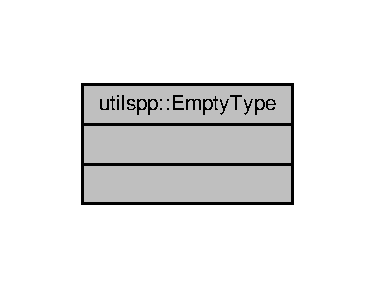
\includegraphics[width=180pt]{structutilspp_1_1EmptyType__coll__graph}
\end{center}
\end{figure}


The documentation for this struct was generated from the following file\-:\begin{DoxyCompactItemize}
\item 
include/utilspp/Empty\-Type.\-hpp\end{DoxyCompactItemize}

\hypertarget{classEmSyRU}{\section{Em\-Sy\-R\-U Class Reference}
\label{classEmSyRU}\index{Em\-Sy\-R\-U@{Em\-Sy\-R\-U}}
}


Class for Emdedded System Remote \hyperlink{classUpdater}{Updater}.  




{\ttfamily \#include $<$Em\-Sy\-R\-U.\-hpp$>$}



Collaboration diagram for Em\-Sy\-R\-U\-:
\nopagebreak
\begin{figure}[H]
\begin{center}
\leavevmode
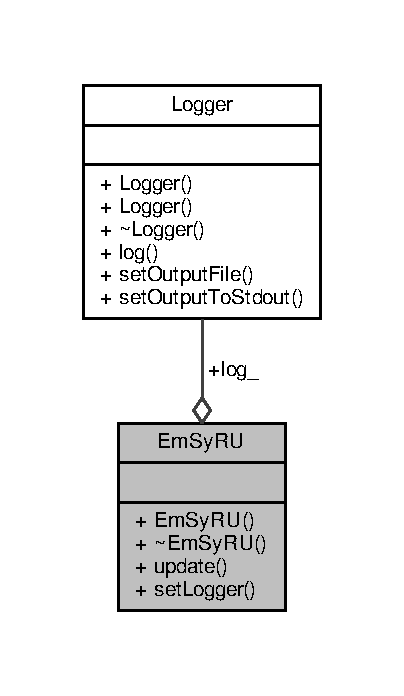
\includegraphics[width=194pt]{classEmSyRU__coll__graph}
\end{center}
\end{figure}
\subsection*{Public Member Functions}
\begin{DoxyCompactItemize}
\item 
\hypertarget{classEmSyRU_ac5d6a38500bc912eba862a14cfb0b1b2}{\hyperlink{classEmSyRU_ac5d6a38500bc912eba862a14cfb0b1b2}{Em\-Sy\-R\-U} (string user, string dl\-U\-R\-L, string pw, string env=\char`\"{}\char`\"{})}\label{classEmSyRU_ac5d6a38500bc912eba862a14cfb0b1b2}

\begin{DoxyCompactList}\small\item\em Ctor. \end{DoxyCompactList}\item 
\hypertarget{classEmSyRU_abad85d79a8bd0176f4a7f95d1df2f03e}{\hyperlink{classEmSyRU_abad85d79a8bd0176f4a7f95d1df2f03e}{$\sim$\-Em\-Sy\-R\-U} ()}\label{classEmSyRU_abad85d79a8bd0176f4a7f95d1df2f03e}

\begin{DoxyCompactList}\small\item\em Dtor. \end{DoxyCompactList}\item 
\hypertarget{classEmSyRU_aeccfb365e5aac8a9b5fee2557645353d}{int {\bfseries update} ()}\label{classEmSyRU_aeccfb365e5aac8a9b5fee2557645353d}

\end{DoxyCompactItemize}
\subsection*{Static Public Member Functions}
\begin{DoxyCompactItemize}
\item 
\hypertarget{classEmSyRU_a2720ea250a00225d5640145fecc66ff2}{static void {\bfseries set\-Logger} (\hyperlink{classLogger}{Logger} \&log)}\label{classEmSyRU_a2720ea250a00225d5640145fecc66ff2}

\end{DoxyCompactItemize}
\subsection*{Static Public Attributes}
\begin{DoxyCompactItemize}
\item 
\hypertarget{classEmSyRU_a63f349fb8a0000e9fec67de2cabfd216}{static \hyperlink{classLogger}{Logger} {\bfseries log\-\_\-} = \hyperlink{classLogger}{Logger}()}\label{classEmSyRU_a63f349fb8a0000e9fec67de2cabfd216}

\end{DoxyCompactItemize}


\subsection{Detailed Description}
Class for Emdedded System Remote \hyperlink{classUpdater}{Updater}. 

The documentation for this class was generated from the following files\-:\begin{DoxyCompactItemize}
\item 
include/\hyperlink{EmSyRU_8hpp}{Em\-Sy\-R\-U.\-hpp}\item 
src/Em\-Sy\-R\-U.\-cpp\end{DoxyCompactItemize}

\hypertarget{structutilspp_1_1tl_1_1erase}{\section{utilspp\-:\-:tl\-:\-:erase$<$ T\-List, T $>$ Struct Template Reference}
\label{structutilspp_1_1tl_1_1erase}\index{utilspp\-::tl\-::erase$<$ T\-List, T $>$@{utilspp\-::tl\-::erase$<$ T\-List, T $>$}}
}


Collaboration diagram for utilspp\-:\-:tl\-:\-:erase$<$ T\-List, T $>$\-:\nopagebreak
\begin{figure}[H]
\begin{center}
\leavevmode
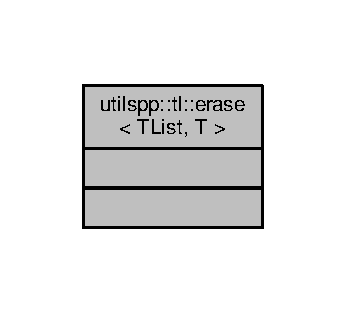
\includegraphics[width=166pt]{structutilspp_1_1tl_1_1erase__coll__graph}
\end{center}
\end{figure}


The documentation for this struct was generated from the following file\-:\begin{DoxyCompactItemize}
\item 
include/utilspp/Type\-List.\-hpp\end{DoxyCompactItemize}

\hypertarget{structutilspp_1_1tl_1_1erase_3_01NullType_00_01T_01_4}{\section{utilspp\-:\-:tl\-:\-:erase$<$ Null\-Type, T $>$ Struct Template Reference}
\label{structutilspp_1_1tl_1_1erase_3_01NullType_00_01T_01_4}\index{utilspp\-::tl\-::erase$<$ Null\-Type, T $>$@{utilspp\-::tl\-::erase$<$ Null\-Type, T $>$}}
}


Collaboration diagram for utilspp\-:\-:tl\-:\-:erase$<$ Null\-Type, T $>$\-:
\nopagebreak
\begin{figure}[H]
\begin{center}
\leavevmode
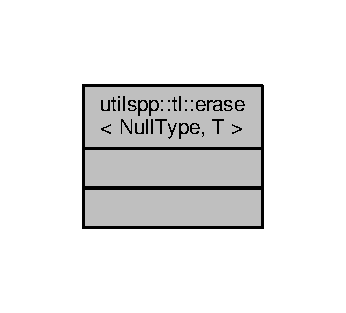
\includegraphics[width=166pt]{structutilspp_1_1tl_1_1erase_3_01NullType_00_01T_01_4__coll__graph}
\end{center}
\end{figure}
\subsection*{Public Types}
\begin{DoxyCompactItemize}
\item 
\hypertarget{structutilspp_1_1tl_1_1erase_3_01NullType_00_01T_01_4_a103804ca2f41beee15f929b435584254}{typedef Null\-Type {\bfseries Result}}\label{structutilspp_1_1tl_1_1erase_3_01NullType_00_01T_01_4_a103804ca2f41beee15f929b435584254}

\end{DoxyCompactItemize}


The documentation for this struct was generated from the following file\-:\begin{DoxyCompactItemize}
\item 
include/utilspp/Type\-List.\-hpp\end{DoxyCompactItemize}

\hypertarget{structutilspp_1_1tl_1_1erase_3_01TypeList_3_01T_00_01TTail_01_4_00_01T_01_4}{\section{utilspp\-:\-:tl\-:\-:erase$<$ Type\-List$<$ T, T\-Tail $>$, T $>$ Struct Template Reference}
\label{structutilspp_1_1tl_1_1erase_3_01TypeList_3_01T_00_01TTail_01_4_00_01T_01_4}\index{utilspp\-::tl\-::erase$<$ Type\-List$<$ T, T\-Tail $>$, T $>$@{utilspp\-::tl\-::erase$<$ Type\-List$<$ T, T\-Tail $>$, T $>$}}
}


Collaboration diagram for utilspp\-:\-:tl\-:\-:erase$<$ Type\-List$<$ T, T\-Tail $>$, T $>$\-:\nopagebreak
\begin{figure}[H]
\begin{center}
\leavevmode
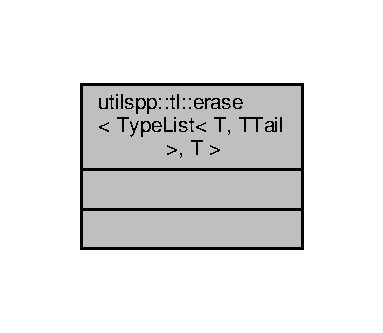
\includegraphics[width=184pt]{structutilspp_1_1tl_1_1erase_3_01TypeList_3_01T_00_01TTail_01_4_00_01T_01_4__coll__graph}
\end{center}
\end{figure}
\subsection*{Public Types}
\begin{DoxyCompactItemize}
\item 
\hypertarget{structutilspp_1_1tl_1_1erase_3_01TypeList_3_01T_00_01TTail_01_4_00_01T_01_4_af3a261a3a865799a2b34bb7521d350c6}{typedef T\-Tail {\bfseries Result}}\label{structutilspp_1_1tl_1_1erase_3_01TypeList_3_01T_00_01TTail_01_4_00_01T_01_4_af3a261a3a865799a2b34bb7521d350c6}

\end{DoxyCompactItemize}


The documentation for this struct was generated from the following file\-:\begin{DoxyCompactItemize}
\item 
include/utilspp/Type\-List.\-hpp\end{DoxyCompactItemize}

\hypertarget{structutilspp_1_1tl_1_1erase_3_01TypeList_3_01THead_00_01TTail_01_4_00_01T_01_4}{\section{utilspp\-:\-:tl\-:\-:erase$<$ Type\-List$<$ T\-Head, T\-Tail $>$, T $>$ Struct Template Reference}
\label{structutilspp_1_1tl_1_1erase_3_01TypeList_3_01THead_00_01TTail_01_4_00_01T_01_4}\index{utilspp\-::tl\-::erase$<$ Type\-List$<$ T\-Head, T\-Tail $>$, T $>$@{utilspp\-::tl\-::erase$<$ Type\-List$<$ T\-Head, T\-Tail $>$, T $>$}}
}


Collaboration diagram for utilspp\-:\-:tl\-:\-:erase$<$ Type\-List$<$ T\-Head, T\-Tail $>$, T $>$\-:
\nopagebreak
\begin{figure}[H]
\begin{center}
\leavevmode
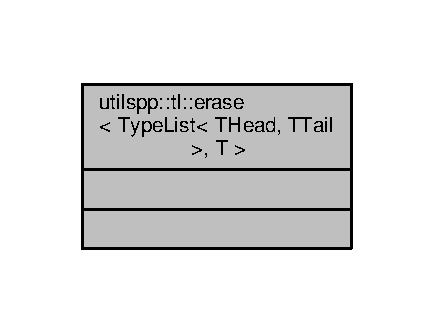
\includegraphics[width=208pt]{structutilspp_1_1tl_1_1erase_3_01TypeList_3_01THead_00_01TTail_01_4_00_01T_01_4__coll__graph}
\end{center}
\end{figure}
\subsection*{Public Types}
\begin{DoxyCompactItemize}
\item 
\hypertarget{structutilspp_1_1tl_1_1erase_3_01TypeList_3_01THead_00_01TTail_01_4_00_01T_01_4_a63196047031f70470bbb9419704f8563}{typedef \hyperlink{structutilspp_1_1tl_1_1TypeList}{Type\-List}$<$ T\-Head, \\*
typename \hyperlink{structutilspp_1_1tl_1_1erase}{erase}$<$ T\-Tail, T $>$\\*
\-::\hyperlink{structutilspp_1_1tl_1_1TypeList}{Result} $>$ {\bfseries Result}}\label{structutilspp_1_1tl_1_1erase_3_01TypeList_3_01THead_00_01TTail_01_4_00_01T_01_4_a63196047031f70470bbb9419704f8563}

\end{DoxyCompactItemize}


The documentation for this struct was generated from the following file\-:\begin{DoxyCompactItemize}
\item 
include/utilspp/Type\-List.\-hpp\end{DoxyCompactItemize}

\hypertarget{classutilspp_1_1FastCount}{\section{utilspp\-:\-:Fast\-Count$<$ Type $>$ Class Template Reference}
\label{classutilspp_1_1FastCount}\index{utilspp\-::\-Fast\-Count$<$ Type $>$@{utilspp\-::\-Fast\-Count$<$ Type $>$}}
}


Collaboration diagram for utilspp\-:\-:Fast\-Count$<$ Type $>$\-:\nopagebreak
\begin{figure}[H]
\begin{center}
\leavevmode
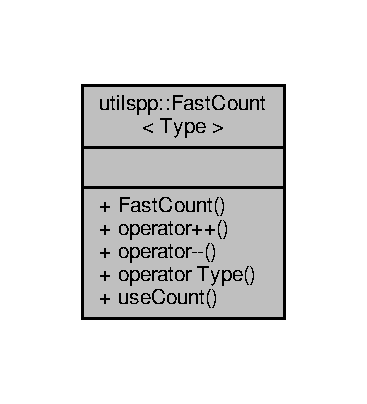
\includegraphics[width=176pt]{classutilspp_1_1FastCount__coll__graph}
\end{center}
\end{figure}
\subsection*{Public Member Functions}
\begin{DoxyCompactItemize}
\item 
\hypertarget{classutilspp_1_1FastCount_aef266176c977bb05093a5a76ff0ccee0}{{\bfseries Fast\-Count} (Type count=1)}\label{classutilspp_1_1FastCount_aef266176c977bb05093a5a76ff0ccee0}

\item 
\hypertarget{classutilspp_1_1FastCount_acbd72fe50f973ddd1c218c5266af218b}{\hyperlink{classutilspp_1_1FastCount}{Fast\-Count} \& {\bfseries operator++} ()}\label{classutilspp_1_1FastCount_acbd72fe50f973ddd1c218c5266af218b}

\item 
\hypertarget{classutilspp_1_1FastCount_ac4dbd8095fc6b8c82f3397199a180dbf}{\hyperlink{classutilspp_1_1FastCount}{Fast\-Count} \& {\bfseries operator-\/-\/} ()}\label{classutilspp_1_1FastCount_ac4dbd8095fc6b8c82f3397199a180dbf}

\item 
\hypertarget{classutilspp_1_1FastCount_aeed9ce68983113d1e74e64c17a4a9705}{{\bfseries operator Type} ()}\label{classutilspp_1_1FastCount_aeed9ce68983113d1e74e64c17a4a9705}

\item 
\hypertarget{classutilspp_1_1FastCount_a0dcf8ab9597e5b96944a0f3db1b7c1ce}{Type {\bfseries use\-Count} ()}\label{classutilspp_1_1FastCount_a0dcf8ab9597e5b96944a0f3db1b7c1ce}

\end{DoxyCompactItemize}


The documentation for this class was generated from the following file\-:\begin{DoxyCompactItemize}
\item 
include/utilspp/Smart\-Ptr.\-hpp\end{DoxyCompactItemize}

\hypertarget{classcurlpp_1_1FormParts_1_1File}{\section{curlpp\-:\-:Form\-Parts\-:\-:File Class Reference}
\label{classcurlpp_1_1FormParts_1_1File}\index{curlpp\-::\-Form\-Parts\-::\-File@{curlpp\-::\-Form\-Parts\-::\-File}}
}


This class is a file post.  




{\ttfamily \#include $<$Form.\-hpp$>$}



Inheritance diagram for curlpp\-:\-:Form\-Parts\-:\-:File\-:
\nopagebreak
\begin{figure}[H]
\begin{center}
\leavevmode
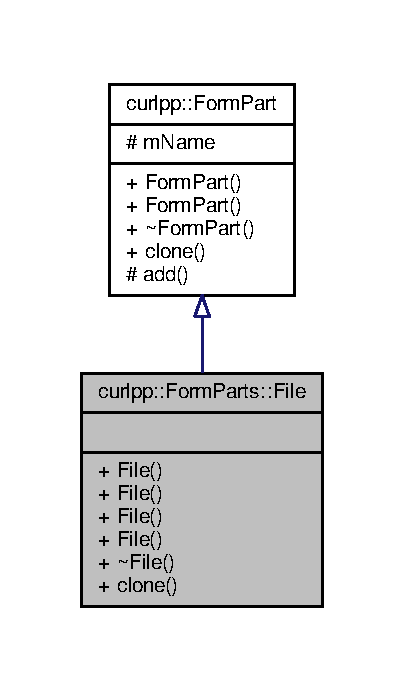
\includegraphics[width=194pt]{classcurlpp_1_1FormParts_1_1File__inherit__graph}
\end{center}
\end{figure}


Collaboration diagram for curlpp\-:\-:Form\-Parts\-:\-:File\-:
\nopagebreak
\begin{figure}[H]
\begin{center}
\leavevmode
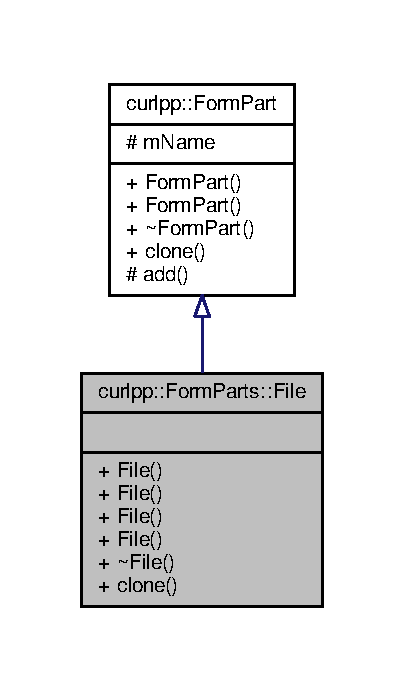
\includegraphics[width=194pt]{classcurlpp_1_1FormParts_1_1File__coll__graph}
\end{center}
\end{figure}
\subsection*{Public Member Functions}
\begin{DoxyCompactItemize}
\item 
\hyperlink{classcurlpp_1_1FormParts_1_1File_a279297fcb9d6f362d432d22363107812}{File} (const char $\ast$name, const char $\ast$filename)
\begin{DoxyCompactList}\small\item\em initialize a \hyperlink{classcurlpp_1_1FormParts_1_1File}{File} part. \end{DoxyCompactList}\item 
\hyperlink{classcurlpp_1_1FormParts_1_1File_a7fd7447d8a4df5d9533ebeb5f3790235}{File} (const char $\ast$name, const char $\ast$filename, const char $\ast$content\-Type)
\begin{DoxyCompactList}\small\item\em initialize a \hyperlink{classcurlpp_1_1FormParts_1_1File}{File} part. \end{DoxyCompactList}\item 
\hyperlink{classcurlpp_1_1FormParts_1_1File_af9054c6b96d284b1ef6dd086b9122b51}{File} (const std\-::string \&name, const std\-::string \&filename)
\begin{DoxyCompactList}\small\item\em initialize a \hyperlink{classcurlpp_1_1FormParts_1_1File}{File} part. \end{DoxyCompactList}\item 
\hyperlink{classcurlpp_1_1FormParts_1_1File_ac961a43be0e8f224f06f71f83bff31fd}{File} (const std\-::string \&name, const std\-::string \&filename, const std\-::string \&content\-Type)
\begin{DoxyCompactList}\small\item\em initialize a \hyperlink{classcurlpp_1_1FormParts_1_1File}{File} part. \end{DoxyCompactList}\item 
\hypertarget{classcurlpp_1_1FormParts_1_1File_ac4917a83ae6f0d039a0e788e0b6c4db8}{virtual \hyperlink{classcurlpp_1_1FormParts_1_1File}{File} $\ast$ \hyperlink{classcurlpp_1_1FormParts_1_1File_ac4917a83ae6f0d039a0e788e0b6c4db8}{clone} () const }\label{classcurlpp_1_1FormParts_1_1File_ac4917a83ae6f0d039a0e788e0b6c4db8}

\begin{DoxyCompactList}\small\item\em This function will return a copy of the instance. \end{DoxyCompactList}\end{DoxyCompactItemize}
\subsection*{Additional Inherited Members}


\subsection{Detailed Description}
This class is a file post. 

It will send a file in the H\-T\-T\-P post. 

\subsection{Constructor \& Destructor Documentation}
\hypertarget{classcurlpp_1_1FormParts_1_1File_a279297fcb9d6f362d432d22363107812}{\index{curlpp\-::\-Form\-Parts\-::\-File@{curlpp\-::\-Form\-Parts\-::\-File}!File@{File}}
\index{File@{File}!curlpp::FormParts::File@{curlpp\-::\-Form\-Parts\-::\-File}}
\subsubsection[{File}]{\setlength{\rightskip}{0pt plus 5cm}curlpp\-::\-Form\-Parts\-::\-File\-::\-File (
\begin{DoxyParamCaption}
\item[{const char $\ast$}]{name, }
\item[{const char $\ast$}]{filename}
\end{DoxyParamCaption}
)}}\label{classcurlpp_1_1FormParts_1_1File_a279297fcb9d6f362d432d22363107812}


initialize a \hyperlink{classcurlpp_1_1FormParts_1_1File}{File} part. 

\char`\"{}name\char`\"{} is the name of the field. \char`\"{}filename\char`\"{} is the string that holds the filename. \hypertarget{classcurlpp_1_1FormParts_1_1File_a7fd7447d8a4df5d9533ebeb5f3790235}{\index{curlpp\-::\-Form\-Parts\-::\-File@{curlpp\-::\-Form\-Parts\-::\-File}!File@{File}}
\index{File@{File}!curlpp::FormParts::File@{curlpp\-::\-Form\-Parts\-::\-File}}
\subsubsection[{File}]{\setlength{\rightskip}{0pt plus 5cm}curlpp\-::\-Form\-Parts\-::\-File\-::\-File (
\begin{DoxyParamCaption}
\item[{const char $\ast$}]{name, }
\item[{const char $\ast$}]{filename, }
\item[{const char $\ast$}]{content\-Type}
\end{DoxyParamCaption}
)}}\label{classcurlpp_1_1FormParts_1_1File_a7fd7447d8a4df5d9533ebeb5f3790235}


initialize a \hyperlink{classcurlpp_1_1FormParts_1_1File}{File} part. 

\char`\"{}name\char`\"{} is the name of the field. \char`\"{}filename\char`\"{} is the string that holds the filename. \char`\"{}content\-Type\char`\"{} is the M\-I\-M\-E type of the file. \hypertarget{classcurlpp_1_1FormParts_1_1File_af9054c6b96d284b1ef6dd086b9122b51}{\index{curlpp\-::\-Form\-Parts\-::\-File@{curlpp\-::\-Form\-Parts\-::\-File}!File@{File}}
\index{File@{File}!curlpp::FormParts::File@{curlpp\-::\-Form\-Parts\-::\-File}}
\subsubsection[{File}]{\setlength{\rightskip}{0pt plus 5cm}curlpp\-::\-Form\-Parts\-::\-File\-::\-File (
\begin{DoxyParamCaption}
\item[{const std\-::string \&}]{name, }
\item[{const std\-::string \&}]{filename}
\end{DoxyParamCaption}
)}}\label{classcurlpp_1_1FormParts_1_1File_af9054c6b96d284b1ef6dd086b9122b51}


initialize a \hyperlink{classcurlpp_1_1FormParts_1_1File}{File} part. 

\char`\"{}name\char`\"{} is the name of the field. \char`\"{}filename\char`\"{} is the string that holds the filename. \hypertarget{classcurlpp_1_1FormParts_1_1File_ac961a43be0e8f224f06f71f83bff31fd}{\index{curlpp\-::\-Form\-Parts\-::\-File@{curlpp\-::\-Form\-Parts\-::\-File}!File@{File}}
\index{File@{File}!curlpp::FormParts::File@{curlpp\-::\-Form\-Parts\-::\-File}}
\subsubsection[{File}]{\setlength{\rightskip}{0pt plus 5cm}curlpp\-::\-Form\-Parts\-::\-File\-::\-File (
\begin{DoxyParamCaption}
\item[{const std\-::string \&}]{name, }
\item[{const std\-::string \&}]{filename, }
\item[{const std\-::string \&}]{content\-Type}
\end{DoxyParamCaption}
)}}\label{classcurlpp_1_1FormParts_1_1File_ac961a43be0e8f224f06f71f83bff31fd}


initialize a \hyperlink{classcurlpp_1_1FormParts_1_1File}{File} part. 

\char`\"{}name\char`\"{} is the name of the field. \char`\"{}filename\char`\"{} is the string that holds the filename. \char`\"{}content\-Type\char`\"{} is the M\-I\-M\-E type of the file. 

The documentation for this class was generated from the following files\-:\begin{DoxyCompactItemize}
\item 
include/curlpp/Form.\-hpp\item 
src/curlpp/Form.\-cpp\end{DoxyCompactItemize}

\hypertarget{classcurlpp_1_1FormPart}{\section{curlpp\-:\-:Form\-Part Class Reference}
\label{classcurlpp_1_1FormPart}\index{curlpp\-::\-Form\-Part@{curlpp\-::\-Form\-Part}}
}


This class is the base representation of a post.  




{\ttfamily \#include $<$Form.\-hpp$>$}



Inheritance diagram for curlpp\-:\-:Form\-Part\-:\nopagebreak
\begin{figure}[H]
\begin{center}
\leavevmode
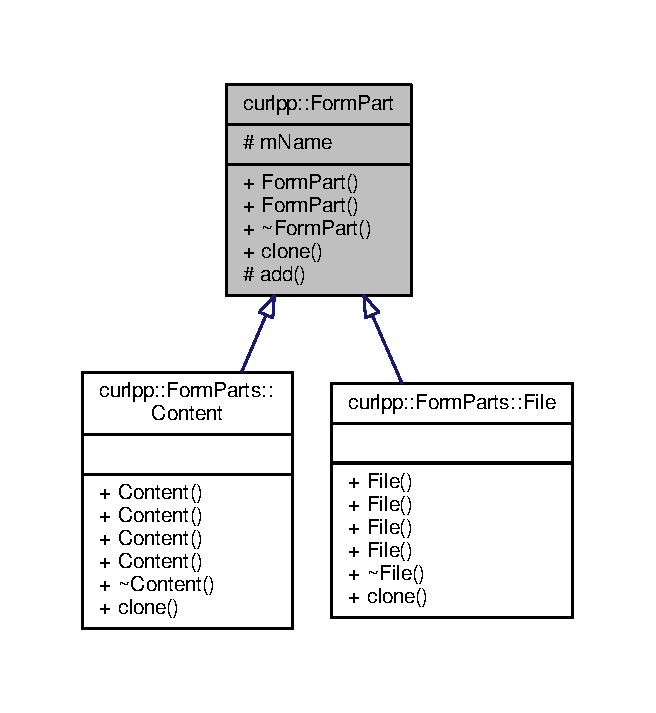
\includegraphics[width=315pt]{classcurlpp_1_1FormPart__inherit__graph}
\end{center}
\end{figure}


Collaboration diagram for curlpp\-:\-:Form\-Part\-:\nopagebreak
\begin{figure}[H]
\begin{center}
\leavevmode
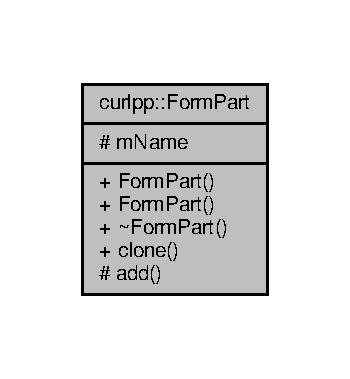
\includegraphics[width=168pt]{classcurlpp_1_1FormPart__coll__graph}
\end{center}
\end{figure}
\subsection*{Public Member Functions}
\begin{DoxyCompactItemize}
\item 
\hyperlink{classcurlpp_1_1FormPart_a25c51c604a32d82d23d2955bb19e2e63}{Form\-Part} (const char $\ast$name)
\begin{DoxyCompactList}\small\item\em initialize the \hyperlink{classcurlpp_1_1FormPart}{Form\-Part}. \end{DoxyCompactList}\item 
\hyperlink{classcurlpp_1_1FormPart_a839ac0adc867bf96ef0b764d8d216850}{Form\-Part} (const std\-::string \&name)
\begin{DoxyCompactList}\small\item\em initialize the \hyperlink{classcurlpp_1_1FormPart}{Form\-Part}. \end{DoxyCompactList}\item 
\hypertarget{classcurlpp_1_1FormPart_a6005cbed5b7e266e280b489bba26e4d1}{virtual \hyperlink{classcurlpp_1_1FormPart}{Form\-Part} $\ast$ {\bfseries clone} () const =0}\label{classcurlpp_1_1FormPart_a6005cbed5b7e266e280b489bba26e4d1}

\end{DoxyCompactItemize}
\subsection*{Protected Member Functions}
\begin{DoxyCompactItemize}
\item 
\hypertarget{classcurlpp_1_1FormPart_ae4f52f30aa0ad2e4cf0a44e6a754b306}{virtual void \hyperlink{classcurlpp_1_1FormPart_ae4f52f30aa0ad2e4cf0a44e6a754b306}{add} (\-::curl\-\_\-httppost $\ast$$\ast$first,\-::curl\-\_\-httppost $\ast$$\ast$last)=0}\label{classcurlpp_1_1FormPart_ae4f52f30aa0ad2e4cf0a44e6a754b306}

\begin{DoxyCompactList}\small\item\em it will add himself to the curl\-\_\-httppost $\ast$ first. \end{DoxyCompactList}\end{DoxyCompactItemize}
\subsection*{Protected Attributes}
\begin{DoxyCompactItemize}
\item 
\hypertarget{classcurlpp_1_1FormPart_a7aa178e7bd1b9322c0a469705e0b6fe5}{const std\-::string \hyperlink{classcurlpp_1_1FormPart_a7aa178e7bd1b9322c0a469705e0b6fe5}{m\-Name}}\label{classcurlpp_1_1FormPart_a7aa178e7bd1b9322c0a469705e0b6fe5}

\begin{DoxyCompactList}\small\item\em Contain the name of the field. \end{DoxyCompactList}\end{DoxyCompactItemize}
\subsection*{Friends}
\begin{DoxyCompactItemize}
\item 
\hypertarget{classcurlpp_1_1FormPart_a12d2180adc694d000dab9af5522a6283}{class {\bfseries Http\-Post}}\label{classcurlpp_1_1FormPart_a12d2180adc694d000dab9af5522a6283}

\end{DoxyCompactItemize}


\subsection{Detailed Description}
This class is the base representation of a post. 

You need to inherit from it to define a type of post. 

\subsection{Constructor \& Destructor Documentation}
\hypertarget{classcurlpp_1_1FormPart_a25c51c604a32d82d23d2955bb19e2e63}{\index{curlpp\-::\-Form\-Part@{curlpp\-::\-Form\-Part}!Form\-Part@{Form\-Part}}
\index{Form\-Part@{Form\-Part}!curlpp::FormPart@{curlpp\-::\-Form\-Part}}
\subsubsection[{Form\-Part}]{\setlength{\rightskip}{0pt plus 5cm}curlpp\-::\-Form\-Part\-::\-Form\-Part (
\begin{DoxyParamCaption}
\item[{const char $\ast$}]{name}
\end{DoxyParamCaption}
)}}\label{classcurlpp_1_1FormPart_a25c51c604a32d82d23d2955bb19e2e63}


initialize the \hyperlink{classcurlpp_1_1FormPart}{Form\-Part}. 

\char`\"{}name\char`\"{} is the name of the field. \hypertarget{classcurlpp_1_1FormPart_a839ac0adc867bf96ef0b764d8d216850}{\index{curlpp\-::\-Form\-Part@{curlpp\-::\-Form\-Part}!Form\-Part@{Form\-Part}}
\index{Form\-Part@{Form\-Part}!curlpp::FormPart@{curlpp\-::\-Form\-Part}}
\subsubsection[{Form\-Part}]{\setlength{\rightskip}{0pt plus 5cm}curlpp\-::\-Form\-Part\-::\-Form\-Part (
\begin{DoxyParamCaption}
\item[{const std\-::string \&}]{name}
\end{DoxyParamCaption}
)}}\label{classcurlpp_1_1FormPart_a839ac0adc867bf96ef0b764d8d216850}


initialize the \hyperlink{classcurlpp_1_1FormPart}{Form\-Part}. 

\char`\"{}name\char`\"{} is the name of the field. 

The documentation for this class was generated from the following files\-:\begin{DoxyCompactItemize}
\item 
include/curlpp/Form.\-hpp\item 
src/curlpp/Form.\-cpp\end{DoxyCompactItemize}

\hypertarget{classutilspp_1_1Functor}{\section{utilspp\-:\-:Functor$<$ R, T\-List $>$ Class Template Reference}
\label{classutilspp_1_1Functor}\index{utilspp\-::\-Functor$<$ R, T\-List $>$@{utilspp\-::\-Functor$<$ R, T\-List $>$}}
}


Collaboration diagram for utilspp\-:\-:Functor$<$ R, T\-List $>$\-:
\nopagebreak
\begin{figure}[H]
\begin{center}
\leavevmode
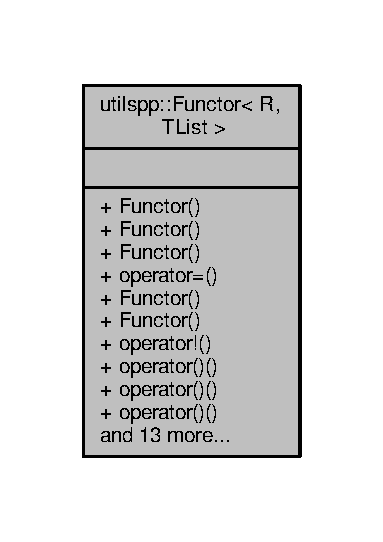
\includegraphics[width=184pt]{classutilspp_1_1Functor__coll__graph}
\end{center}
\end{figure}
\subsection*{Public Types}
\begin{DoxyCompactItemize}
\item 
\hypertarget{classutilspp_1_1Functor_a99a2e43a2eeed54dd40beb515914a9a2}{typedef \hyperlink{structutilspp_1_1FunctorImpl}{Functor\-Impl}$<$ R, T\-List $>$ {\bfseries Impl}}\label{classutilspp_1_1Functor_a99a2e43a2eeed54dd40beb515914a9a2}

\item 
\hypertarget{classutilspp_1_1Functor_a5542a47c91adb5810d22d34d29bee730}{typedef R {\bfseries Result\-Type}}\label{classutilspp_1_1Functor_a5542a47c91adb5810d22d34d29bee730}

\item 
\hypertarget{classutilspp_1_1Functor_a881db21cf78bfafa5690736ff332e431}{typedef T\-List {\bfseries Parm\-List}}\label{classutilspp_1_1Functor_a881db21cf78bfafa5690736ff332e431}

\item 
\hypertarget{classutilspp_1_1Functor_a588ae828cc0497982c437da15d3f22a9}{typedef \\*
\hyperlink{structutilspp_1_1tl_1_1TypeAtNonStrict}{utilspp\-::tl\-::\-Type\-At\-Non\-Strict}\\*
$<$ T\-List, 0, \hyperlink{structutilspp_1_1EmptyType}{utilspp\-::\-Empty\-Type} $>$\\*
\-::Result {\bfseries Parm1}}\label{classutilspp_1_1Functor_a588ae828cc0497982c437da15d3f22a9}

\item 
\hypertarget{classutilspp_1_1Functor_a5c7eb4c2a8c04533701440011387e879}{typedef \\*
\hyperlink{structutilspp_1_1tl_1_1TypeAtNonStrict}{utilspp\-::tl\-::\-Type\-At\-Non\-Strict}\\*
$<$ T\-List, 1, \hyperlink{structutilspp_1_1EmptyType}{utilspp\-::\-Empty\-Type} $>$\\*
\-::Result {\bfseries Parm2}}\label{classutilspp_1_1Functor_a5c7eb4c2a8c04533701440011387e879}

\item 
\hypertarget{classutilspp_1_1Functor_ab963c72c0eb58654b2b6b6502ffc6440}{typedef \\*
\hyperlink{structutilspp_1_1tl_1_1TypeAtNonStrict}{utilspp\-::tl\-::\-Type\-At\-Non\-Strict}\\*
$<$ T\-List, 2, \hyperlink{structutilspp_1_1EmptyType}{utilspp\-::\-Empty\-Type} $>$\\*
\-::Result {\bfseries Parm3}}\label{classutilspp_1_1Functor_ab963c72c0eb58654b2b6b6502ffc6440}

\item 
\hypertarget{classutilspp_1_1Functor_a56d44a1be8a03de2f036a9b198558d77}{typedef \\*
\hyperlink{structutilspp_1_1tl_1_1TypeAtNonStrict}{utilspp\-::tl\-::\-Type\-At\-Non\-Strict}\\*
$<$ T\-List, 3, \hyperlink{structutilspp_1_1EmptyType}{utilspp\-::\-Empty\-Type} $>$\\*
\-::Result {\bfseries Parm4}}\label{classutilspp_1_1Functor_a56d44a1be8a03de2f036a9b198558d77}

\item 
\hypertarget{classutilspp_1_1Functor_a91709579a2ecef614a365cb7210caf94}{typedef \\*
\hyperlink{structutilspp_1_1tl_1_1TypeAtNonStrict}{utilspp\-::tl\-::\-Type\-At\-Non\-Strict}\\*
$<$ T\-List, 4, \hyperlink{structutilspp_1_1EmptyType}{utilspp\-::\-Empty\-Type} $>$\\*
\-::Result {\bfseries Parm5}}\label{classutilspp_1_1Functor_a91709579a2ecef614a365cb7210caf94}

\item 
\hypertarget{classutilspp_1_1Functor_a501aab6ad009739cdc17bd74ef839211}{typedef \\*
\hyperlink{structutilspp_1_1tl_1_1TypeAtNonStrict}{utilspp\-::tl\-::\-Type\-At\-Non\-Strict}\\*
$<$ T\-List, 5, \hyperlink{structutilspp_1_1EmptyType}{utilspp\-::\-Empty\-Type} $>$\\*
\-::Result {\bfseries Parm6}}\label{classutilspp_1_1Functor_a501aab6ad009739cdc17bd74ef839211}

\item 
\hypertarget{classutilspp_1_1Functor_a3b37dab0a8dccad781846fe9db72fdb1}{typedef \\*
\hyperlink{structutilspp_1_1tl_1_1TypeAtNonStrict}{utilspp\-::tl\-::\-Type\-At\-Non\-Strict}\\*
$<$ T\-List, 6, \hyperlink{structutilspp_1_1EmptyType}{utilspp\-::\-Empty\-Type} $>$\\*
\-::Result {\bfseries Parm7}}\label{classutilspp_1_1Functor_a3b37dab0a8dccad781846fe9db72fdb1}

\item 
\hypertarget{classutilspp_1_1Functor_aca03cd1997d5d15e1badd6dd1b661c75}{typedef \\*
\hyperlink{structutilspp_1_1tl_1_1TypeAtNonStrict}{utilspp\-::tl\-::\-Type\-At\-Non\-Strict}\\*
$<$ T\-List, 7, \hyperlink{structutilspp_1_1EmptyType}{utilspp\-::\-Empty\-Type} $>$\\*
\-::Result {\bfseries Parm8}}\label{classutilspp_1_1Functor_aca03cd1997d5d15e1badd6dd1b661c75}

\item 
\hypertarget{classutilspp_1_1Functor_a2a7e33db462c352b67f1864a94785894}{typedef \\*
\hyperlink{structutilspp_1_1tl_1_1TypeAtNonStrict}{utilspp\-::tl\-::\-Type\-At\-Non\-Strict}\\*
$<$ T\-List, 8, \hyperlink{structutilspp_1_1EmptyType}{utilspp\-::\-Empty\-Type} $>$\\*
\-::Result {\bfseries Parm9}}\label{classutilspp_1_1Functor_a2a7e33db462c352b67f1864a94785894}

\item 
\hypertarget{classutilspp_1_1Functor_ab92e9ee3213f0e86868da6397ba8c21d}{typedef \\*
\hyperlink{structutilspp_1_1tl_1_1TypeAtNonStrict}{utilspp\-::tl\-::\-Type\-At\-Non\-Strict}\\*
$<$ T\-List, 9, \hyperlink{structutilspp_1_1EmptyType}{utilspp\-::\-Empty\-Type} $>$\\*
\-::Result {\bfseries Parm10}}\label{classutilspp_1_1Functor_ab92e9ee3213f0e86868da6397ba8c21d}

\item 
\hypertarget{classutilspp_1_1Functor_a69606918d71735876989b90f01464574}{typedef \\*
\hyperlink{structutilspp_1_1tl_1_1TypeAtNonStrict}{utilspp\-::tl\-::\-Type\-At\-Non\-Strict}\\*
$<$ T\-List, \\*
10, \hyperlink{structutilspp_1_1EmptyType}{utilspp\-::\-Empty\-Type} $>$\\*
\-::Result {\bfseries Parm11}}\label{classutilspp_1_1Functor_a69606918d71735876989b90f01464574}

\item 
\hypertarget{classutilspp_1_1Functor_a5553f0833ffa3284cd6d8f0987bb8650}{typedef \\*
\hyperlink{structutilspp_1_1tl_1_1TypeAtNonStrict}{utilspp\-::tl\-::\-Type\-At\-Non\-Strict}\\*
$<$ T\-List, \\*
11, \hyperlink{structutilspp_1_1EmptyType}{utilspp\-::\-Empty\-Type} $>$\\*
\-::Result {\bfseries Parm12}}\label{classutilspp_1_1Functor_a5553f0833ffa3284cd6d8f0987bb8650}

\item 
\hypertarget{classutilspp_1_1Functor_a28e37e932741fa110de33527da9cb869}{typedef \\*
\hyperlink{structutilspp_1_1tl_1_1TypeAtNonStrict}{utilspp\-::tl\-::\-Type\-At\-Non\-Strict}\\*
$<$ T\-List, \\*
12, \hyperlink{structutilspp_1_1EmptyType}{utilspp\-::\-Empty\-Type} $>$\\*
\-::Result {\bfseries Parm13}}\label{classutilspp_1_1Functor_a28e37e932741fa110de33527da9cb869}

\item 
\hypertarget{classutilspp_1_1Functor_a1cb28ac257f68e75e1bcdc6c63d23351}{typedef \\*
\hyperlink{structutilspp_1_1tl_1_1TypeAtNonStrict}{utilspp\-::tl\-::\-Type\-At\-Non\-Strict}\\*
$<$ T\-List, \\*
13, \hyperlink{structutilspp_1_1EmptyType}{utilspp\-::\-Empty\-Type} $>$\\*
\-::Result {\bfseries Parm14}}\label{classutilspp_1_1Functor_a1cb28ac257f68e75e1bcdc6c63d23351}

\item 
\hypertarget{classutilspp_1_1Functor_a33952917bb039e0ab723147a9611b57d}{typedef \\*
\hyperlink{structutilspp_1_1tl_1_1TypeAtNonStrict}{utilspp\-::tl\-::\-Type\-At\-Non\-Strict}\\*
$<$ T\-List, \\*
14, \hyperlink{structutilspp_1_1EmptyType}{utilspp\-::\-Empty\-Type} $>$\\*
\-::Result {\bfseries Parm15}}\label{classutilspp_1_1Functor_a33952917bb039e0ab723147a9611b57d}

\end{DoxyCompactItemize}
\subsection*{Public Member Functions}
\begin{DoxyCompactItemize}
\item 
\hypertarget{classutilspp_1_1Functor_abf122492569cda6af15291161b126231}{{\bfseries Functor} (const \hyperlink{classutilspp_1_1Functor}{Functor} \&functor)}\label{classutilspp_1_1Functor_abf122492569cda6af15291161b126231}

\item 
\hypertarget{classutilspp_1_1Functor_a22717724866552dd02dac01a98c09d32}{{\bfseries Functor} (std\-::auto\-\_\-ptr$<$ \hyperlink{structutilspp_1_1FunctorImpl}{Impl} $>$ impl)}\label{classutilspp_1_1Functor_a22717724866552dd02dac01a98c09d32}

\item 
\hypertarget{classutilspp_1_1Functor_a4f711f224934efa997c1fb4891a7f3a1}{\hyperlink{classutilspp_1_1Functor}{Functor} \& {\bfseries operator=} (const \hyperlink{classutilspp_1_1Functor}{Functor} \&functor)}\label{classutilspp_1_1Functor_a4f711f224934efa997c1fb4891a7f3a1}

\item 
\hypertarget{classutilspp_1_1Functor_ad3cb9001426794b33ae05f6cf3cdc512}{{\footnotesize template$<$class Fun $>$ }\\{\bfseries Functor} (Fun fun)}\label{classutilspp_1_1Functor_ad3cb9001426794b33ae05f6cf3cdc512}

\item 
\hypertarget{classutilspp_1_1Functor_a55a2998649d016f9e25f445052b02286}{{\footnotesize template$<$class Pointer\-To\-Obj , class Mem\-Fun $>$ }\\{\bfseries Functor} (const Pointer\-To\-Obj \&obj, Mem\-Fun fun)}\label{classutilspp_1_1Functor_a55a2998649d016f9e25f445052b02286}

\item 
\hypertarget{classutilspp_1_1Functor_a5d481f1869bd55882e87b0c4e648ee5f}{bool {\bfseries operator!} ()}\label{classutilspp_1_1Functor_a5d481f1869bd55882e87b0c4e648ee5f}

\item 
\hypertarget{classutilspp_1_1Functor_a446508160326c6258a84d154669f66f9}{R {\bfseries operator()} ()}\label{classutilspp_1_1Functor_a446508160326c6258a84d154669f66f9}

\item 
\hypertarget{classutilspp_1_1Functor_a3f32c90ebea10b1effacb09f4b690999}{R {\bfseries operator()} (Parm1 p1)}\label{classutilspp_1_1Functor_a3f32c90ebea10b1effacb09f4b690999}

\item 
\hypertarget{classutilspp_1_1Functor_a70021698a0ea099c4ede1c1c8bd31ad4}{R {\bfseries operator()} (Parm1 p1, Parm2 p2)}\label{classutilspp_1_1Functor_a70021698a0ea099c4ede1c1c8bd31ad4}

\item 
\hypertarget{classutilspp_1_1Functor_a19a69482d56402f234f4fedcab15a8d3}{R {\bfseries operator()} (Parm1 p1, Parm2 p2, Parm3 p3)}\label{classutilspp_1_1Functor_a19a69482d56402f234f4fedcab15a8d3}

\item 
\hypertarget{classutilspp_1_1Functor_a0ffc3b96e5a995fd6b39677d6f9e2a9e}{R {\bfseries operator()} (Parm1 p1, Parm2 p2, Parm3 p3, Parm4 p4)}\label{classutilspp_1_1Functor_a0ffc3b96e5a995fd6b39677d6f9e2a9e}

\item 
\hypertarget{classutilspp_1_1Functor_a51d835c88961a0f2cc163fdde77a67d7}{R {\bfseries operator()} (Parm1 p1, Parm2 p2, Parm3 p3, Parm4 p4, Parm5 p5)}\label{classutilspp_1_1Functor_a51d835c88961a0f2cc163fdde77a67d7}

\item 
\hypertarget{classutilspp_1_1Functor_a53c6b262b5dff629e8f0eb8d452bb9ed}{R {\bfseries operator()} (Parm1 p1, Parm2 p2, Parm3 p3, Parm4 p4, Parm5 p5, Parm6 p6)}\label{classutilspp_1_1Functor_a53c6b262b5dff629e8f0eb8d452bb9ed}

\item 
\hypertarget{classutilspp_1_1Functor_ad23373e50777351bcbe55530eff1450e}{R {\bfseries operator()} (Parm1 p1, Parm2 p2, Parm3 p3, Parm4 p4, Parm5 p5, Parm6 p6, Parm7 p7)}\label{classutilspp_1_1Functor_ad23373e50777351bcbe55530eff1450e}

\item 
\hypertarget{classutilspp_1_1Functor_aea3a0677a840ff772a23a1acdb7903dc}{R {\bfseries operator()} (Parm1 p1, Parm2 p2, Parm3 p3, Parm4 p4, Parm5 p5, Parm6 p6, Parm7 p7, Parm8 p8)}\label{classutilspp_1_1Functor_aea3a0677a840ff772a23a1acdb7903dc}

\item 
\hypertarget{classutilspp_1_1Functor_a8baf7f11731c14c4b665096050bf80e8}{R {\bfseries operator()} (Parm1 p1, Parm2 p2, Parm3 p3, Parm4 p4, Parm5 p5, Parm6 p6, Parm7 p7, Parm8 p8, Parm9 p9)}\label{classutilspp_1_1Functor_a8baf7f11731c14c4b665096050bf80e8}

\item 
\hypertarget{classutilspp_1_1Functor_a32472ed540582980ad17b4473414204e}{R {\bfseries operator()} (Parm1 p1, Parm2 p2, Parm3 p3, Parm4 p4, Parm5 p5, Parm6 p6, Parm7 p7, Parm8 p8, Parm9 p9, Parm10 p10)}\label{classutilspp_1_1Functor_a32472ed540582980ad17b4473414204e}

\item 
\hypertarget{classutilspp_1_1Functor_af142c2d8213ad7c45bd9d9f1f0f0789c}{R {\bfseries operator()} (Parm1 p1, Parm2 p2, Parm3 p3, Parm4 p4, Parm5 p5, Parm6 p6, Parm7 p7, Parm8 p8, Parm9 p9, Parm10 p10, Parm11 p11)}\label{classutilspp_1_1Functor_af142c2d8213ad7c45bd9d9f1f0f0789c}

\item 
\hypertarget{classutilspp_1_1Functor_a137a728e1c6b12b89d760f8440067c5a}{R {\bfseries operator()} (Parm1 p1, Parm2 p2, Parm3 p3, Parm4 p4, Parm5 p5, Parm6 p6, Parm7 p7, Parm8 p8, Parm9 p9, Parm10 p10, Parm11 p11, Parm12 p12)}\label{classutilspp_1_1Functor_a137a728e1c6b12b89d760f8440067c5a}

\item 
\hypertarget{classutilspp_1_1Functor_a58df5cae9e0cf66ee3d8d5c3a8e7e18e}{R {\bfseries operator()} (Parm1 p1, Parm2 p2, Parm3 p3, Parm4 p4, Parm5 p5, Parm6 p6, Parm7 p7, Parm8 p8, Parm9 p9, Parm10 p10, Parm11 p11, Parm12 p12, Parm13 p13)}\label{classutilspp_1_1Functor_a58df5cae9e0cf66ee3d8d5c3a8e7e18e}

\item 
\hypertarget{classutilspp_1_1Functor_a09e6761a67513d2365b9e443869b0c2b}{R {\bfseries operator()} (Parm1 p1, Parm2 p2, Parm3 p3, Parm4 p4, Parm5 p5, Parm6 p6, Parm7 p7, Parm8 p8, Parm9 p9, Parm10 p10, Parm11 p11, Parm12 p12, Parm13 p13, Parm14 p14)}\label{classutilspp_1_1Functor_a09e6761a67513d2365b9e443869b0c2b}

\item 
\hypertarget{classutilspp_1_1Functor_adc37428ffbe848078e9a1b2c7331770a}{R {\bfseries operator()} (Parm1 p1, Parm2 p2, Parm3 p3, Parm4 p4, Parm5 p5, Parm6 p6, Parm7 p7, Parm8 p8, Parm9 p9, Parm10 p10, Parm11 p11, Parm12 p12, Parm13 p13, Parm14 p14, Parm15 p15)}\label{classutilspp_1_1Functor_adc37428ffbe848078e9a1b2c7331770a}

\end{DoxyCompactItemize}


The documentation for this class was generated from the following file\-:\begin{DoxyCompactItemize}
\item 
include/utilspp/functor/Functor.\-hpp\end{DoxyCompactItemize}

\hypertarget{classutilspp_1_1FunctorHandler}{\section{utilspp\-:\-:Functor\-Handler$<$ Parent\-Functor, Fun $>$ Class Template Reference}
\label{classutilspp_1_1FunctorHandler}\index{utilspp\-::\-Functor\-Handler$<$ Parent\-Functor, Fun $>$@{utilspp\-::\-Functor\-Handler$<$ Parent\-Functor, Fun $>$}}
}


Inheritance diagram for utilspp\-:\-:Functor\-Handler$<$ Parent\-Functor, Fun $>$\-:\nopagebreak
\begin{figure}[H]
\begin{center}
\leavevmode
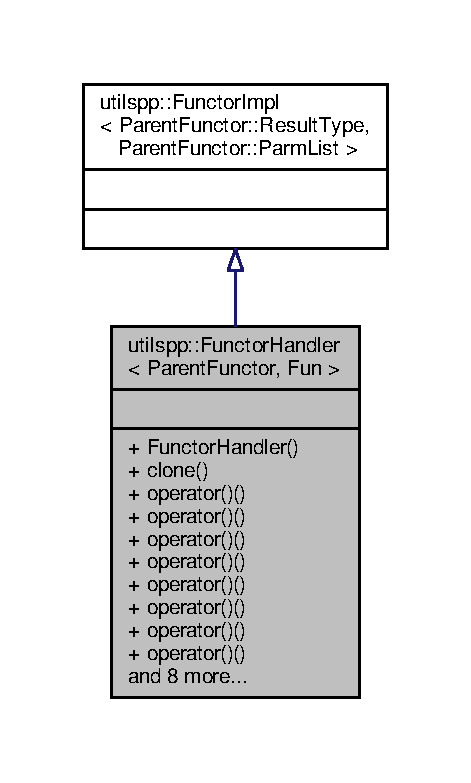
\includegraphics[width=226pt]{classutilspp_1_1FunctorHandler__inherit__graph}
\end{center}
\end{figure}


Collaboration diagram for utilspp\-:\-:Functor\-Handler$<$ Parent\-Functor, Fun $>$\-:\nopagebreak
\begin{figure}[H]
\begin{center}
\leavevmode
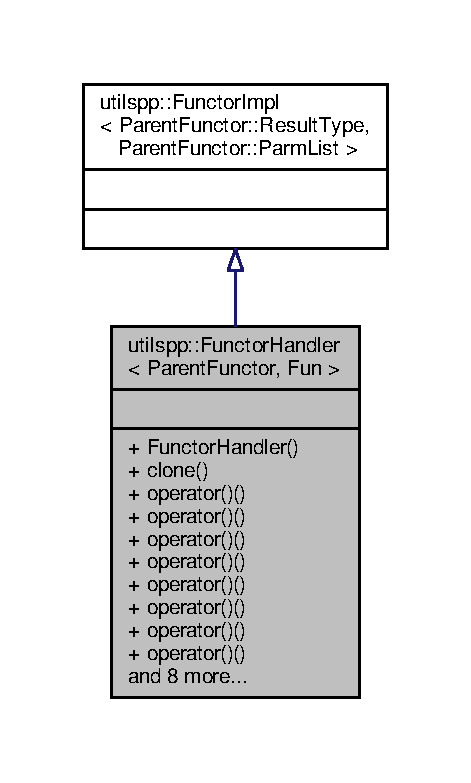
\includegraphics[width=226pt]{classutilspp_1_1FunctorHandler__coll__graph}
\end{center}
\end{figure}
\subsection*{Public Types}
\begin{DoxyCompactItemize}
\item 
\hypertarget{classutilspp_1_1FunctorHandler_ac1582c39cb3d20184679a1b17039fb8a}{typedef Parent\-Functor\-::\-Result\-Type {\bfseries Result\-Type}}\label{classutilspp_1_1FunctorHandler_ac1582c39cb3d20184679a1b17039fb8a}

\end{DoxyCompactItemize}
\subsection*{Public Member Functions}
\begin{DoxyCompactItemize}
\item 
\hypertarget{classutilspp_1_1FunctorHandler_a51626d2b3812b75b8c599b6af0b03248}{{\bfseries Functor\-Handler} (Fun fun)}\label{classutilspp_1_1FunctorHandler_a51626d2b3812b75b8c599b6af0b03248}

\item 
\hypertarget{classutilspp_1_1FunctorHandler_a656e2e439733ea62a323da708d40abca}{\hyperlink{classutilspp_1_1FunctorHandler}{Functor\-Handler} $\ast$ {\bfseries clone} () const }\label{classutilspp_1_1FunctorHandler_a656e2e439733ea62a323da708d40abca}

\item 
\hypertarget{classutilspp_1_1FunctorHandler_a0a33055a2db431cbe0db5e4d8476e074}{Result\-Type {\bfseries operator()} ()}\label{classutilspp_1_1FunctorHandler_a0a33055a2db431cbe0db5e4d8476e074}

\item 
\hypertarget{classutilspp_1_1FunctorHandler_a18844d204f2ed519cf5d7f1e303fabee}{Result\-Type {\bfseries operator()} (typename Parent\-Functor\-::\-Parm1 p1)}\label{classutilspp_1_1FunctorHandler_a18844d204f2ed519cf5d7f1e303fabee}

\item 
\hypertarget{classutilspp_1_1FunctorHandler_adb36146996463b68fd5c2b6a6b910624}{Result\-Type {\bfseries operator()} (typename Parent\-Functor\-::\-Parm1 p1, typename Parent\-Functor\-::\-Parm2 p2)}\label{classutilspp_1_1FunctorHandler_adb36146996463b68fd5c2b6a6b910624}

\item 
\hypertarget{classutilspp_1_1FunctorHandler_a425f53a4c5db48e9a96341e6020172e9}{Result\-Type {\bfseries operator()} (typename Parent\-Functor\-::\-Parm1 p1, typename Parent\-Functor\-::\-Parm2 p2, typename Parent\-Functor\-::\-Parm3 p3)}\label{classutilspp_1_1FunctorHandler_a425f53a4c5db48e9a96341e6020172e9}

\item 
\hypertarget{classutilspp_1_1FunctorHandler_af0d43ca57ea4938d67e23b69cd291b15}{Result\-Type {\bfseries operator()} (typename Parent\-Functor\-::\-Parm1 p1, typename Parent\-Functor\-::\-Parm2 p2, typename Parent\-Functor\-::\-Parm3 p3, typename Parent\-Functor\-::\-Parm4 p4)}\label{classutilspp_1_1FunctorHandler_af0d43ca57ea4938d67e23b69cd291b15}

\item 
\hypertarget{classutilspp_1_1FunctorHandler_aceecbbdc3e511628bf8dfc9b2e793a78}{Result\-Type {\bfseries operator()} (typename Parent\-Functor\-::\-Parm1 p1, typename Parent\-Functor\-::\-Parm2 p2, typename Parent\-Functor\-::\-Parm3 p3, typename Parent\-Functor\-::\-Parm4 p4, typename Parent\-Functor\-::\-Parm5 p5)}\label{classutilspp_1_1FunctorHandler_aceecbbdc3e511628bf8dfc9b2e793a78}

\item 
\hypertarget{classutilspp_1_1FunctorHandler_a3e690c68eafd010febde6d2e187434e0}{Result\-Type {\bfseries operator()} (typename Parent\-Functor\-::\-Parm1 p1, typename Parent\-Functor\-::\-Parm2 p2, typename Parent\-Functor\-::\-Parm3 p3, typename Parent\-Functor\-::\-Parm4 p4, typename Parent\-Functor\-::\-Parm5 p5, typename Parent\-Functor\-::\-Parm6 p6)}\label{classutilspp_1_1FunctorHandler_a3e690c68eafd010febde6d2e187434e0}

\item 
\hypertarget{classutilspp_1_1FunctorHandler_a7e89906c96d718119105f5cfa413e030}{Result\-Type {\bfseries operator()} (typename Parent\-Functor\-::\-Parm1 p1, typename Parent\-Functor\-::\-Parm2 p2, typename Parent\-Functor\-::\-Parm3 p3, typename Parent\-Functor\-::\-Parm4 p4, typename Parent\-Functor\-::\-Parm5 p5, typename Parent\-Functor\-::\-Parm6 p6, typename Parent\-Functor\-::\-Parm7 p7)}\label{classutilspp_1_1FunctorHandler_a7e89906c96d718119105f5cfa413e030}

\item 
\hypertarget{classutilspp_1_1FunctorHandler_a0a76f5205c35d55636601169e7a8d482}{Result\-Type {\bfseries operator()} (typename Parent\-Functor\-::\-Parm1 p1, typename Parent\-Functor\-::\-Parm2 p2, typename Parent\-Functor\-::\-Parm3 p3, typename Parent\-Functor\-::\-Parm4 p4, typename Parent\-Functor\-::\-Parm5 p5, typename Parent\-Functor\-::\-Parm6 p6, typename Parent\-Functor\-::\-Parm7 p7, typename Parent\-Functor\-::\-Parm8 p8)}\label{classutilspp_1_1FunctorHandler_a0a76f5205c35d55636601169e7a8d482}

\item 
\hypertarget{classutilspp_1_1FunctorHandler_aae7f1882c3416f6297f6c732c4433c49}{Result\-Type {\bfseries operator()} (typename Parent\-Functor\-::\-Parm1 p1, typename Parent\-Functor\-::\-Parm2 p2, typename Parent\-Functor\-::\-Parm3 p3, typename Parent\-Functor\-::\-Parm4 p4, typename Parent\-Functor\-::\-Parm5 p5, typename Parent\-Functor\-::\-Parm6 p6, typename Parent\-Functor\-::\-Parm7 p7, typename Parent\-Functor\-::\-Parm8 p8, typename Parent\-Functor\-::\-Parm9 p9)}\label{classutilspp_1_1FunctorHandler_aae7f1882c3416f6297f6c732c4433c49}

\item 
\hypertarget{classutilspp_1_1FunctorHandler_a2acd007b15dbbb96efc10f7fcf2e88ad}{Result\-Type {\bfseries operator()} (typename Parent\-Functor\-::\-Parm1 p1, typename Parent\-Functor\-::\-Parm2 p2, typename Parent\-Functor\-::\-Parm3 p3, typename Parent\-Functor\-::\-Parm4 p4, typename Parent\-Functor\-::\-Parm5 p5, typename Parent\-Functor\-::\-Parm6 p6, typename Parent\-Functor\-::\-Parm7 p7, typename Parent\-Functor\-::\-Parm8 p8, typename Parent\-Functor\-::\-Parm9 p9, typename Parent\-Functor\-::\-Parm10 p10)}\label{classutilspp_1_1FunctorHandler_a2acd007b15dbbb96efc10f7fcf2e88ad}

\item 
\hypertarget{classutilspp_1_1FunctorHandler_a0e909e7046ab7f74dcd5c28077999e58}{Result\-Type {\bfseries operator()} (typename Parent\-Functor\-::\-Parm1 p1, typename Parent\-Functor\-::\-Parm2 p2, typename Parent\-Functor\-::\-Parm3 p3, typename Parent\-Functor\-::\-Parm4 p4, typename Parent\-Functor\-::\-Parm5 p5, typename Parent\-Functor\-::\-Parm6 p6, typename Parent\-Functor\-::\-Parm7 p7, typename Parent\-Functor\-::\-Parm8 p8, typename Parent\-Functor\-::\-Parm9 p9, typename Parent\-Functor\-::\-Parm10 p10, typename Parent\-Functor\-::\-Parm11 p11)}\label{classutilspp_1_1FunctorHandler_a0e909e7046ab7f74dcd5c28077999e58}

\item 
\hypertarget{classutilspp_1_1FunctorHandler_aa8879b1e73cdc78612cffa19e7458d8e}{Result\-Type {\bfseries operator()} (typename Parent\-Functor\-::\-Parm1 p1, typename Parent\-Functor\-::\-Parm2 p2, typename Parent\-Functor\-::\-Parm3 p3, typename Parent\-Functor\-::\-Parm4 p4, typename Parent\-Functor\-::\-Parm5 p5, typename Parent\-Functor\-::\-Parm6 p6, typename Parent\-Functor\-::\-Parm7 p7, typename Parent\-Functor\-::\-Parm8 p8, typename Parent\-Functor\-::\-Parm9 p9, typename Parent\-Functor\-::\-Parm10 p10, typename Parent\-Functor\-::\-Parm11 p11, typename Parent\-Functor\-::\-Parm12 p12)}\label{classutilspp_1_1FunctorHandler_aa8879b1e73cdc78612cffa19e7458d8e}

\item 
\hypertarget{classutilspp_1_1FunctorHandler_a1d92a68fec979a2ad613c63a55a0dddc}{Result\-Type {\bfseries operator()} (typename Parent\-Functor\-::\-Parm1 p1, typename Parent\-Functor\-::\-Parm2 p2, typename Parent\-Functor\-::\-Parm3 p3, typename Parent\-Functor\-::\-Parm4 p4, typename Parent\-Functor\-::\-Parm5 p5, typename Parent\-Functor\-::\-Parm6 p6, typename Parent\-Functor\-::\-Parm7 p7, typename Parent\-Functor\-::\-Parm8 p8, typename Parent\-Functor\-::\-Parm9 p9, typename Parent\-Functor\-::\-Parm10 p10, typename Parent\-Functor\-::\-Parm11 p11, typename Parent\-Functor\-::\-Parm12 p12, typename Parent\-Functor\-::\-Parm13 p13)}\label{classutilspp_1_1FunctorHandler_a1d92a68fec979a2ad613c63a55a0dddc}

\item 
\hypertarget{classutilspp_1_1FunctorHandler_a0272e78f3272dd4cd2871a1c082006a8}{Result\-Type {\bfseries operator()} (typename Parent\-Functor\-::\-Parm1 p1, typename Parent\-Functor\-::\-Parm2 p2, typename Parent\-Functor\-::\-Parm3 p3, typename Parent\-Functor\-::\-Parm4 p4, typename Parent\-Functor\-::\-Parm5 p5, typename Parent\-Functor\-::\-Parm6 p6, typename Parent\-Functor\-::\-Parm7 p7, typename Parent\-Functor\-::\-Parm8 p8, typename Parent\-Functor\-::\-Parm9 p9, typename Parent\-Functor\-::\-Parm10 p10, typename Parent\-Functor\-::\-Parm11 p11, typename Parent\-Functor\-::\-Parm12 p12, typename Parent\-Functor\-::\-Parm13 p13, typename Parent\-Functor\-::\-Parm14 p14)}\label{classutilspp_1_1FunctorHandler_a0272e78f3272dd4cd2871a1c082006a8}

\item 
\hypertarget{classutilspp_1_1FunctorHandler_a5fe82645dbb655281aab8474553dd87a}{Result\-Type {\bfseries operator()} (typename Parent\-Functor\-::\-Parm1 p1, typename Parent\-Functor\-::\-Parm2 p2, typename Parent\-Functor\-::\-Parm3 p3, typename Parent\-Functor\-::\-Parm4 p4, typename Parent\-Functor\-::\-Parm5 p5, typename Parent\-Functor\-::\-Parm6 p6, typename Parent\-Functor\-::\-Parm7 p7, typename Parent\-Functor\-::\-Parm8 p8, typename Parent\-Functor\-::\-Parm9 p9, typename Parent\-Functor\-::\-Parm10 p10, typename Parent\-Functor\-::\-Parm11 p11, typename Parent\-Functor\-::\-Parm12 p12, typename Parent\-Functor\-::\-Parm13 p13, typename Parent\-Functor\-::\-Parm14 p14, typename Parent\-Functor\-::\-Parm15 p15)}\label{classutilspp_1_1FunctorHandler_a5fe82645dbb655281aab8474553dd87a}

\end{DoxyCompactItemize}


The documentation for this class was generated from the following file\-:\begin{DoxyCompactItemize}
\item 
include/utilspp/functor/Functor\-Handler.\-hpp\end{DoxyCompactItemize}

\hypertarget{structutilspp_1_1FunctorImpl}{\section{utilspp\-:\-:Functor\-Impl$<$ R, T\-List $>$ Struct Template Reference}
\label{structutilspp_1_1FunctorImpl}\index{utilspp\-::\-Functor\-Impl$<$ R, T\-List $>$@{utilspp\-::\-Functor\-Impl$<$ R, T\-List $>$}}
}


Collaboration diagram for utilspp\-:\-:Functor\-Impl$<$ R, T\-List $>$\-:\nopagebreak
\begin{figure}[H]
\begin{center}
\leavevmode
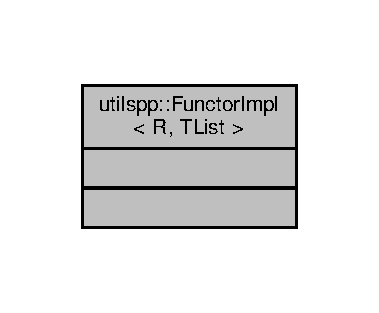
\includegraphics[width=182pt]{structutilspp_1_1FunctorImpl__coll__graph}
\end{center}
\end{figure}


The documentation for this struct was generated from the following file\-:\begin{DoxyCompactItemize}
\item 
include/utilspp/functor/Functor\-Impl.\-hpp\end{DoxyCompactItemize}

\hypertarget{structutilspp_1_1FunctorImpl_3_01R_00_01TYPE__LIST__1_07P1_08_4}{\section{utilspp\-:\-:Functor\-Impl$<$ R, T\-Y\-P\-E\-\_\-\-L\-I\-S\-T\-\_\-1(P1)$>$ Struct Template Reference}
\label{structutilspp_1_1FunctorImpl_3_01R_00_01TYPE__LIST__1_07P1_08_4}\index{utilspp\-::\-Functor\-Impl$<$ R, T\-Y\-P\-E\-\_\-\-L\-I\-S\-T\-\_\-1(\-P1)$>$@{utilspp\-::\-Functor\-Impl$<$ R, T\-Y\-P\-E\-\_\-\-L\-I\-S\-T\-\_\-1(\-P1)$>$}}
}


Collaboration diagram for utilspp\-:\-:Functor\-Impl$<$ R, T\-Y\-P\-E\-\_\-\-L\-I\-S\-T\-\_\-1(P1)$>$\-:
\nopagebreak
\begin{figure}[H]
\begin{center}
\leavevmode
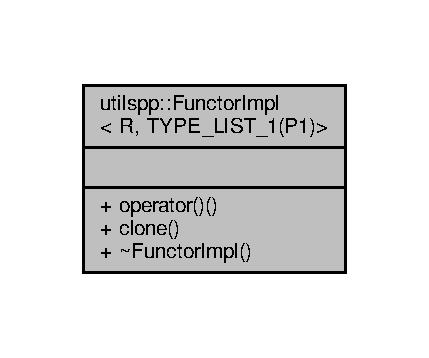
\includegraphics[width=206pt]{structutilspp_1_1FunctorImpl_3_01R_00_01TYPE__LIST__1_07P1_08_4__coll__graph}
\end{center}
\end{figure}
\subsection*{Public Member Functions}
\begin{DoxyCompactItemize}
\item 
\hypertarget{structutilspp_1_1FunctorImpl_3_01R_00_01TYPE__LIST__1_07P1_08_4_abf621bfda0afeb269275de7972a5c779}{virtual R {\bfseries operator()} (P1)=0}\label{structutilspp_1_1FunctorImpl_3_01R_00_01TYPE__LIST__1_07P1_08_4_abf621bfda0afeb269275de7972a5c779}

\item 
\hypertarget{structutilspp_1_1FunctorImpl_3_01R_00_01TYPE__LIST__1_07P1_08_4_aae926b6655a4b24e0321a64a8343e5e6}{virtual \hyperlink{structutilspp_1_1FunctorImpl}{Functor\-Impl} $\ast$ {\bfseries clone} () const =0}\label{structutilspp_1_1FunctorImpl_3_01R_00_01TYPE__LIST__1_07P1_08_4_aae926b6655a4b24e0321a64a8343e5e6}

\end{DoxyCompactItemize}


The documentation for this struct was generated from the following file\-:\begin{DoxyCompactItemize}
\item 
include/utilspp/functor/Functor\-Impl.\-hpp\end{DoxyCompactItemize}

\hypertarget{structutilspp_1_1FunctorImpl_3_01R_00_01TYPE__LIST__10_07P1_00_01P2_00_01P3_00_01P4_00_01P5_00_0dcb5930806c25abd002b833487c3746a}{\section{utilspp\-:\-:Functor\-Impl$<$ R, T\-Y\-P\-E\-\_\-\-L\-I\-S\-T\-\_\-10(P1, P2, P3, P4, P5, P6, P7, P8, P9, P10)$>$ Struct Template Reference}
\label{structutilspp_1_1FunctorImpl_3_01R_00_01TYPE__LIST__10_07P1_00_01P2_00_01P3_00_01P4_00_01P5_00_0dcb5930806c25abd002b833487c3746a}\index{utilspp\-::\-Functor\-Impl$<$ R, T\-Y\-P\-E\-\_\-\-L\-I\-S\-T\-\_\-10(\-P1, P2, P3, P4, P5, P6, P7, P8, P9, P10)$>$@{utilspp\-::\-Functor\-Impl$<$ R, T\-Y\-P\-E\-\_\-\-L\-I\-S\-T\-\_\-10(\-P1, P2, P3, P4, P5, P6, P7, P8, P9, P10)$>$}}
}


Collaboration diagram for utilspp\-:\-:Functor\-Impl$<$ R, T\-Y\-P\-E\-\_\-\-L\-I\-S\-T\-\_\-10(P1, P2, P3, P4, P5, P6, P7, P8, P9, P10)$>$\-:\nopagebreak
\begin{figure}[H]
\begin{center}
\leavevmode
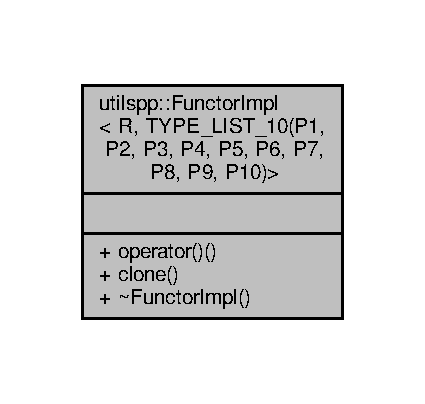
\includegraphics[width=204pt]{structutilspp_1_1FunctorImpl_3_01R_00_01TYPE__LIST__10_07P1_00_01P2_00_01P3_00_01P4_00_01P5_00_0c8371b2be0f819f634b09b6aafbc3c27}
\end{center}
\end{figure}
\subsection*{Public Member Functions}
\begin{DoxyCompactItemize}
\item 
\hypertarget{structutilspp_1_1FunctorImpl_3_01R_00_01TYPE__LIST__10_07P1_00_01P2_00_01P3_00_01P4_00_01P5_00_0dcb5930806c25abd002b833487c3746a_aa30c8cd1173e54081d8ff77f539f6bb0}{virtual R {\bfseries operator()} (P1, P2, P3, P4, P5, P6, P7, P8, P9, P10)=0}\label{structutilspp_1_1FunctorImpl_3_01R_00_01TYPE__LIST__10_07P1_00_01P2_00_01P3_00_01P4_00_01P5_00_0dcb5930806c25abd002b833487c3746a_aa30c8cd1173e54081d8ff77f539f6bb0}

\item 
\hypertarget{structutilspp_1_1FunctorImpl_3_01R_00_01TYPE__LIST__10_07P1_00_01P2_00_01P3_00_01P4_00_01P5_00_0dcb5930806c25abd002b833487c3746a_a255f703c81d7fcf46376a23568fae31b}{virtual \hyperlink{structutilspp_1_1FunctorImpl}{Functor\-Impl} $\ast$ {\bfseries clone} () const =0}\label{structutilspp_1_1FunctorImpl_3_01R_00_01TYPE__LIST__10_07P1_00_01P2_00_01P3_00_01P4_00_01P5_00_0dcb5930806c25abd002b833487c3746a_a255f703c81d7fcf46376a23568fae31b}

\end{DoxyCompactItemize}


The documentation for this struct was generated from the following file\-:\begin{DoxyCompactItemize}
\item 
include/utilspp/functor/Functor\-Impl.\-hpp\end{DoxyCompactItemize}

\hypertarget{structutilspp_1_1FunctorImpl_3_01R_00_01TYPE__LIST__11_07P1_00_01P2_00_01P3_00_01P4_00_01P5_00_02390a23e4d9e9c3c4133bb7a8d48a2c0}{\section{utilspp\-:\-:Functor\-Impl$<$ R, T\-Y\-P\-E\-\_\-\-L\-I\-S\-T\-\_\-11(P1, P2, P3, P4, P5, P6, P7, P8, P9, P10, P11)$>$ Struct Template Reference}
\label{structutilspp_1_1FunctorImpl_3_01R_00_01TYPE__LIST__11_07P1_00_01P2_00_01P3_00_01P4_00_01P5_00_02390a23e4d9e9c3c4133bb7a8d48a2c0}\index{utilspp\-::\-Functor\-Impl$<$ R, T\-Y\-P\-E\-\_\-\-L\-I\-S\-T\-\_\-11(\-P1, P2, P3, P4, P5, P6, P7, P8, P9, P10, P11)$>$@{utilspp\-::\-Functor\-Impl$<$ R, T\-Y\-P\-E\-\_\-\-L\-I\-S\-T\-\_\-11(\-P1, P2, P3, P4, P5, P6, P7, P8, P9, P10, P11)$>$}}
}


Collaboration diagram for utilspp\-:\-:Functor\-Impl$<$ R, T\-Y\-P\-E\-\_\-\-L\-I\-S\-T\-\_\-11(P1, P2, P3, P4, P5, P6, P7, P8, P9, P10, P11)$>$\-:
\nopagebreak
\begin{figure}[H]
\begin{center}
\leavevmode
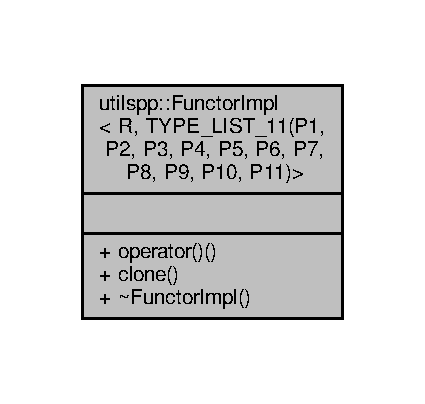
\includegraphics[width=204pt]{structutilspp_1_1FunctorImpl_3_01R_00_01TYPE__LIST__11_07P1_00_01P2_00_01P3_00_01P4_00_01P5_00_08053957277ae9681bf1c10b376e5d869}
\end{center}
\end{figure}
\subsection*{Public Member Functions}
\begin{DoxyCompactItemize}
\item 
\hypertarget{structutilspp_1_1FunctorImpl_3_01R_00_01TYPE__LIST__11_07P1_00_01P2_00_01P3_00_01P4_00_01P5_00_02390a23e4d9e9c3c4133bb7a8d48a2c0_a73bbaa0f525b8af8d3103cd5ead17356}{virtual R {\bfseries operator()} (P1, P2, P3, P4, P5, P6, P7, P8, P9, P10, P11)=0}\label{structutilspp_1_1FunctorImpl_3_01R_00_01TYPE__LIST__11_07P1_00_01P2_00_01P3_00_01P4_00_01P5_00_02390a23e4d9e9c3c4133bb7a8d48a2c0_a73bbaa0f525b8af8d3103cd5ead17356}

\item 
\hypertarget{structutilspp_1_1FunctorImpl_3_01R_00_01TYPE__LIST__11_07P1_00_01P2_00_01P3_00_01P4_00_01P5_00_02390a23e4d9e9c3c4133bb7a8d48a2c0_ab16a312028f180e5552bb9fc9f15f451}{virtual \hyperlink{structutilspp_1_1FunctorImpl}{Functor\-Impl} $\ast$ {\bfseries clone} () const =0}\label{structutilspp_1_1FunctorImpl_3_01R_00_01TYPE__LIST__11_07P1_00_01P2_00_01P3_00_01P4_00_01P5_00_02390a23e4d9e9c3c4133bb7a8d48a2c0_ab16a312028f180e5552bb9fc9f15f451}

\end{DoxyCompactItemize}


The documentation for this struct was generated from the following file\-:\begin{DoxyCompactItemize}
\item 
include/utilspp/functor/Functor\-Impl.\-hpp\end{DoxyCompactItemize}

\hypertarget{structutilspp_1_1FunctorImpl_3_01R_00_01TYPE__LIST__12_07P1_00_01P2_00_01P3_00_01P4_00_01P5_00_0f8d0c7f7e384c45bf768264cb987d1dc}{\section{utilspp\-:\-:Functor\-Impl$<$ R, T\-Y\-P\-E\-\_\-\-L\-I\-S\-T\-\_\-12(P1, P2, P3, P4, P5, P6, P7, P8, P9, P10, P11, P12)$>$ Struct Template Reference}
\label{structutilspp_1_1FunctorImpl_3_01R_00_01TYPE__LIST__12_07P1_00_01P2_00_01P3_00_01P4_00_01P5_00_0f8d0c7f7e384c45bf768264cb987d1dc}\index{utilspp\-::\-Functor\-Impl$<$ R, T\-Y\-P\-E\-\_\-\-L\-I\-S\-T\-\_\-12(\-P1, P2, P3, P4, P5, P6, P7, P8, P9, P10, P11, P12)$>$@{utilspp\-::\-Functor\-Impl$<$ R, T\-Y\-P\-E\-\_\-\-L\-I\-S\-T\-\_\-12(\-P1, P2, P3, P4, P5, P6, P7, P8, P9, P10, P11, P12)$>$}}
}


Collaboration diagram for utilspp\-:\-:Functor\-Impl$<$ R, T\-Y\-P\-E\-\_\-\-L\-I\-S\-T\-\_\-12(P1, P2, P3, P4, P5, P6, P7, P8, P9, P10, P11, P12)$>$\-:\nopagebreak
\begin{figure}[H]
\begin{center}
\leavevmode
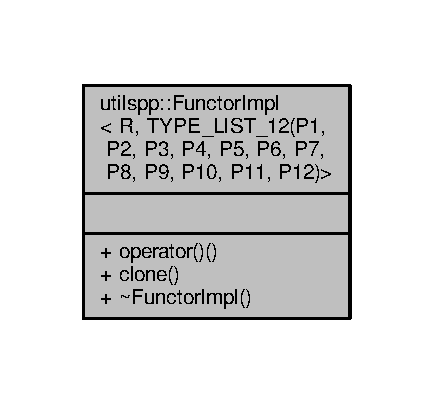
\includegraphics[width=208pt]{structutilspp_1_1FunctorImpl_3_01R_00_01TYPE__LIST__12_07P1_00_01P2_00_01P3_00_01P4_00_01P5_00_01fda986fbaa63d8271f174d79261ea4b}
\end{center}
\end{figure}
\subsection*{Public Member Functions}
\begin{DoxyCompactItemize}
\item 
\hypertarget{structutilspp_1_1FunctorImpl_3_01R_00_01TYPE__LIST__12_07P1_00_01P2_00_01P3_00_01P4_00_01P5_00_0f8d0c7f7e384c45bf768264cb987d1dc_a08b5220edca2cc9ea88fcda264ece482}{virtual R {\bfseries operator()} (P1, P2, P3, P4, P5, P6, P7, P8, P9, P10, P11, P12)=0}\label{structutilspp_1_1FunctorImpl_3_01R_00_01TYPE__LIST__12_07P1_00_01P2_00_01P3_00_01P4_00_01P5_00_0f8d0c7f7e384c45bf768264cb987d1dc_a08b5220edca2cc9ea88fcda264ece482}

\item 
\hypertarget{structutilspp_1_1FunctorImpl_3_01R_00_01TYPE__LIST__12_07P1_00_01P2_00_01P3_00_01P4_00_01P5_00_0f8d0c7f7e384c45bf768264cb987d1dc_a9583c953b349595ccb736ad13bec1d6f}{virtual \hyperlink{structutilspp_1_1FunctorImpl}{Functor\-Impl} $\ast$ {\bfseries clone} () const =0}\label{structutilspp_1_1FunctorImpl_3_01R_00_01TYPE__LIST__12_07P1_00_01P2_00_01P3_00_01P4_00_01P5_00_0f8d0c7f7e384c45bf768264cb987d1dc_a9583c953b349595ccb736ad13bec1d6f}

\end{DoxyCompactItemize}


The documentation for this struct was generated from the following file\-:\begin{DoxyCompactItemize}
\item 
include/utilspp/functor/Functor\-Impl.\-hpp\end{DoxyCompactItemize}

\hypertarget{structutilspp_1_1FunctorImpl_3_01R_00_01TYPE__LIST__13_07P1_00_01P2_00_01P3_00_01P4_00_01P5_00_0c958a377a1633cfded06d0625afe62c5}{\section{utilspp\-:\-:Functor\-Impl$<$ R, T\-Y\-P\-E\-\_\-\-L\-I\-S\-T\-\_\-13(P1, P2, P3, P4, P5, P6, P7, P8, P9, P10, P11, P12, P13)$>$ Struct Template Reference}
\label{structutilspp_1_1FunctorImpl_3_01R_00_01TYPE__LIST__13_07P1_00_01P2_00_01P3_00_01P4_00_01P5_00_0c958a377a1633cfded06d0625afe62c5}\index{utilspp\-::\-Functor\-Impl$<$ R, T\-Y\-P\-E\-\_\-\-L\-I\-S\-T\-\_\-13(\-P1, P2, P3, P4, P5, P6, P7, P8, P9, P10, P11, P12, P13)$>$@{utilspp\-::\-Functor\-Impl$<$ R, T\-Y\-P\-E\-\_\-\-L\-I\-S\-T\-\_\-13(\-P1, P2, P3, P4, P5, P6, P7, P8, P9, P10, P11, P12, P13)$>$}}
}


Collaboration diagram for utilspp\-:\-:Functor\-Impl$<$ R, T\-Y\-P\-E\-\_\-\-L\-I\-S\-T\-\_\-13(P1, P2, P3, P4, P5, P6, P7, P8, P9, P10, P11, P12, P13)$>$\-:
\nopagebreak
\begin{figure}[H]
\begin{center}
\leavevmode
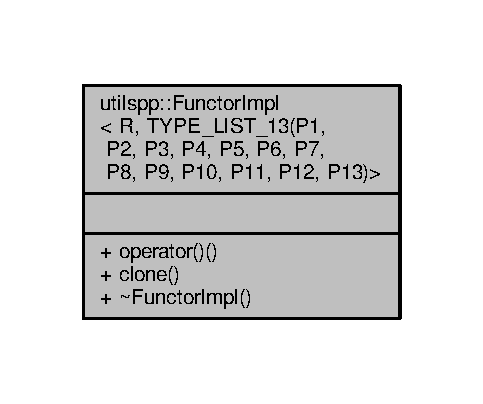
\includegraphics[width=232pt]{structutilspp_1_1FunctorImpl_3_01R_00_01TYPE__LIST__13_07P1_00_01P2_00_01P3_00_01P4_00_01P5_00_0449d2a2be1bee786ba21febad7177958}
\end{center}
\end{figure}
\subsection*{Public Member Functions}
\begin{DoxyCompactItemize}
\item 
\hypertarget{structutilspp_1_1FunctorImpl_3_01R_00_01TYPE__LIST__13_07P1_00_01P2_00_01P3_00_01P4_00_01P5_00_0c958a377a1633cfded06d0625afe62c5_a6a95e9f3b9b281cbe20fcb3bb2a458ee}{virtual R {\bfseries operator()} (P1, P2, P3, P4, P5, P6, P7, P8, P9, P10, P11, P12, P13)=0}\label{structutilspp_1_1FunctorImpl_3_01R_00_01TYPE__LIST__13_07P1_00_01P2_00_01P3_00_01P4_00_01P5_00_0c958a377a1633cfded06d0625afe62c5_a6a95e9f3b9b281cbe20fcb3bb2a458ee}

\item 
\hypertarget{structutilspp_1_1FunctorImpl_3_01R_00_01TYPE__LIST__13_07P1_00_01P2_00_01P3_00_01P4_00_01P5_00_0c958a377a1633cfded06d0625afe62c5_ae28b57b5d13dbd0d0493318edf4282a9}{virtual \hyperlink{structutilspp_1_1FunctorImpl}{Functor\-Impl} $\ast$ {\bfseries clone} () const =0}\label{structutilspp_1_1FunctorImpl_3_01R_00_01TYPE__LIST__13_07P1_00_01P2_00_01P3_00_01P4_00_01P5_00_0c958a377a1633cfded06d0625afe62c5_ae28b57b5d13dbd0d0493318edf4282a9}

\end{DoxyCompactItemize}


The documentation for this struct was generated from the following file\-:\begin{DoxyCompactItemize}
\item 
include/utilspp/functor/Functor\-Impl.\-hpp\end{DoxyCompactItemize}

\hypertarget{structutilspp_1_1FunctorImpl_3_01R_00_01TYPE__LIST__14_07P1_00_01P2_00_01P3_00_01P4_00_01P5_00_068b9945896861b079e861dc8bbcfbe94}{\section{utilspp\-:\-:Functor\-Impl$<$ R, T\-Y\-P\-E\-\_\-\-L\-I\-S\-T\-\_\-14(P1, P2, P3, P4, P5, P6, P7, P8, P9, P10, P11, P12, P13, P14)$>$ Struct Template Reference}
\label{structutilspp_1_1FunctorImpl_3_01R_00_01TYPE__LIST__14_07P1_00_01P2_00_01P3_00_01P4_00_01P5_00_068b9945896861b079e861dc8bbcfbe94}\index{utilspp\-::\-Functor\-Impl$<$ R, T\-Y\-P\-E\-\_\-\-L\-I\-S\-T\-\_\-14(\-P1, P2, P3, P4, P5, P6, P7, P8, P9, P10, P11, P12, P13, P14)$>$@{utilspp\-::\-Functor\-Impl$<$ R, T\-Y\-P\-E\-\_\-\-L\-I\-S\-T\-\_\-14(\-P1, P2, P3, P4, P5, P6, P7, P8, P9, P10, P11, P12, P13, P14)$>$}}
}


Collaboration diagram for utilspp\-:\-:Functor\-Impl$<$ R, T\-Y\-P\-E\-\_\-\-L\-I\-S\-T\-\_\-14(P1, P2, P3, P4, P5, P6, P7, P8, P9, P10, P11, P12, P13, P14)$>$\-:
\nopagebreak
\begin{figure}[H]
\begin{center}
\leavevmode
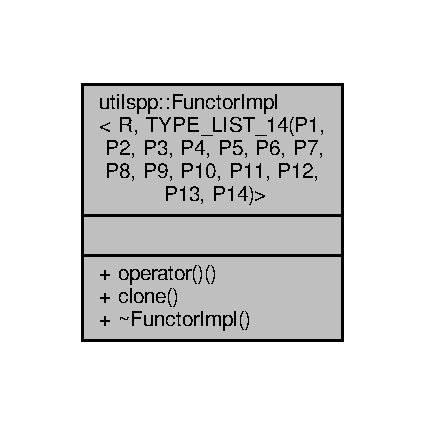
\includegraphics[width=204pt]{structutilspp_1_1FunctorImpl_3_01R_00_01TYPE__LIST__14_07P1_00_01P2_00_01P3_00_01P4_00_01P5_00_0b0404484014de1058783e20f736fdade}
\end{center}
\end{figure}
\subsection*{Public Member Functions}
\begin{DoxyCompactItemize}
\item 
\hypertarget{structutilspp_1_1FunctorImpl_3_01R_00_01TYPE__LIST__14_07P1_00_01P2_00_01P3_00_01P4_00_01P5_00_068b9945896861b079e861dc8bbcfbe94_a852ce71eb8a2e6adfc5a7ff27df5fd84}{virtual R {\bfseries operator()} (P1, P2, P3, P4, P5, P6, P7, P8, P9, P10, P11, P12, P13, P14)=0}\label{structutilspp_1_1FunctorImpl_3_01R_00_01TYPE__LIST__14_07P1_00_01P2_00_01P3_00_01P4_00_01P5_00_068b9945896861b079e861dc8bbcfbe94_a852ce71eb8a2e6adfc5a7ff27df5fd84}

\item 
\hypertarget{structutilspp_1_1FunctorImpl_3_01R_00_01TYPE__LIST__14_07P1_00_01P2_00_01P3_00_01P4_00_01P5_00_068b9945896861b079e861dc8bbcfbe94_aa0713e401193291caa187a792d10e7a9}{virtual \hyperlink{structutilspp_1_1FunctorImpl}{Functor\-Impl} $\ast$ {\bfseries clone} () const =0}\label{structutilspp_1_1FunctorImpl_3_01R_00_01TYPE__LIST__14_07P1_00_01P2_00_01P3_00_01P4_00_01P5_00_068b9945896861b079e861dc8bbcfbe94_aa0713e401193291caa187a792d10e7a9}

\end{DoxyCompactItemize}


The documentation for this struct was generated from the following file\-:\begin{DoxyCompactItemize}
\item 
include/utilspp/functor/Functor\-Impl.\-hpp\end{DoxyCompactItemize}

\hypertarget{structutilspp_1_1FunctorImpl_3_01R_00_01TYPE__LIST__15_07P1_00_01P2_00_01P3_00_01P4_00_01P5_00_03f6bfb72f2977866a35a5dbc6e440ab4}{\section{utilspp\-:\-:Functor\-Impl$<$ R, T\-Y\-P\-E\-\_\-\-L\-I\-S\-T\-\_\-15(P1, P2, P3, P4, P5, P6, P7, P8, P9, P10, P11, P12, P13, P14, P15)$>$ Struct Template Reference}
\label{structutilspp_1_1FunctorImpl_3_01R_00_01TYPE__LIST__15_07P1_00_01P2_00_01P3_00_01P4_00_01P5_00_03f6bfb72f2977866a35a5dbc6e440ab4}\index{utilspp\-::\-Functor\-Impl$<$ R, T\-Y\-P\-E\-\_\-\-L\-I\-S\-T\-\_\-15(\-P1, P2, P3, P4, P5, P6, P7, P8, P9, P10, P11, P12, P13, P14, P15)$>$@{utilspp\-::\-Functor\-Impl$<$ R, T\-Y\-P\-E\-\_\-\-L\-I\-S\-T\-\_\-15(\-P1, P2, P3, P4, P5, P6, P7, P8, P9, P10, P11, P12, P13, P14, P15)$>$}}
}


Collaboration diagram for utilspp\-:\-:Functor\-Impl$<$ R, T\-Y\-P\-E\-\_\-\-L\-I\-S\-T\-\_\-15(P1, P2, P3, P4, P5, P6, P7, P8, P9, P10, P11, P12, P13, P14, P15)$>$\-:
\nopagebreak
\begin{figure}[H]
\begin{center}
\leavevmode
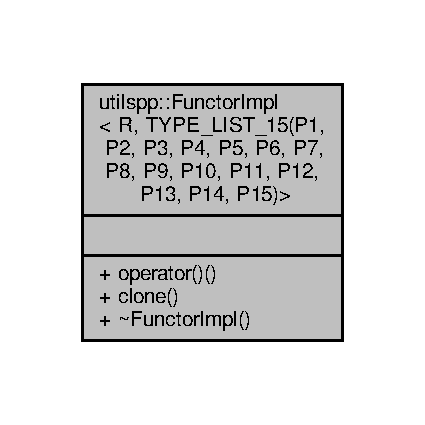
\includegraphics[width=204pt]{structutilspp_1_1FunctorImpl_3_01R_00_01TYPE__LIST__15_07P1_00_01P2_00_01P3_00_01P4_00_01P5_00_08a89af694afbd983ff661781d76f97f6}
\end{center}
\end{figure}
\subsection*{Public Member Functions}
\begin{DoxyCompactItemize}
\item 
\hypertarget{structutilspp_1_1FunctorImpl_3_01R_00_01TYPE__LIST__15_07P1_00_01P2_00_01P3_00_01P4_00_01P5_00_03f6bfb72f2977866a35a5dbc6e440ab4_ac4a0898f96f5b288e1993b64bef6c431}{virtual R {\bfseries operator()} (P1, P2, P3, P4, P5, P6, P7, P8, P9, P10, P11, P12, P13, P14, P15)=0}\label{structutilspp_1_1FunctorImpl_3_01R_00_01TYPE__LIST__15_07P1_00_01P2_00_01P3_00_01P4_00_01P5_00_03f6bfb72f2977866a35a5dbc6e440ab4_ac4a0898f96f5b288e1993b64bef6c431}

\item 
\hypertarget{structutilspp_1_1FunctorImpl_3_01R_00_01TYPE__LIST__15_07P1_00_01P2_00_01P3_00_01P4_00_01P5_00_03f6bfb72f2977866a35a5dbc6e440ab4_a3f0a230f65762069b13c4cb18921f419}{virtual \hyperlink{structutilspp_1_1FunctorImpl}{Functor\-Impl} $\ast$ {\bfseries clone} () const =0}\label{structutilspp_1_1FunctorImpl_3_01R_00_01TYPE__LIST__15_07P1_00_01P2_00_01P3_00_01P4_00_01P5_00_03f6bfb72f2977866a35a5dbc6e440ab4_a3f0a230f65762069b13c4cb18921f419}

\end{DoxyCompactItemize}


The documentation for this struct was generated from the following file\-:\begin{DoxyCompactItemize}
\item 
include/utilspp/functor/Functor\-Impl.\-hpp\end{DoxyCompactItemize}

\hypertarget{structutilspp_1_1FunctorImpl_3_01R_00_01TYPE__LIST__2_07P1_00_01P2_08_4}{\section{utilspp\-:\-:Functor\-Impl$<$ R, T\-Y\-P\-E\-\_\-\-L\-I\-S\-T\-\_\-2(P1, P2)$>$ Struct Template Reference}
\label{structutilspp_1_1FunctorImpl_3_01R_00_01TYPE__LIST__2_07P1_00_01P2_08_4}\index{utilspp\-::\-Functor\-Impl$<$ R, T\-Y\-P\-E\-\_\-\-L\-I\-S\-T\-\_\-2(\-P1, P2)$>$@{utilspp\-::\-Functor\-Impl$<$ R, T\-Y\-P\-E\-\_\-\-L\-I\-S\-T\-\_\-2(\-P1, P2)$>$}}
}


Collaboration diagram for utilspp\-:\-:Functor\-Impl$<$ R, T\-Y\-P\-E\-\_\-\-L\-I\-S\-T\-\_\-2(P1, P2)$>$\-:
\nopagebreak
\begin{figure}[H]
\begin{center}
\leavevmode
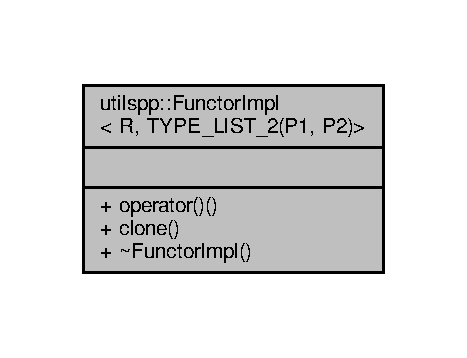
\includegraphics[width=224pt]{structutilspp_1_1FunctorImpl_3_01R_00_01TYPE__LIST__2_07P1_00_01P2_08_4__coll__graph}
\end{center}
\end{figure}
\subsection*{Public Member Functions}
\begin{DoxyCompactItemize}
\item 
\hypertarget{structutilspp_1_1FunctorImpl_3_01R_00_01TYPE__LIST__2_07P1_00_01P2_08_4_a6c37e9ecec518bb01543781b67143407}{virtual R {\bfseries operator()} (P1, P2)=0}\label{structutilspp_1_1FunctorImpl_3_01R_00_01TYPE__LIST__2_07P1_00_01P2_08_4_a6c37e9ecec518bb01543781b67143407}

\item 
\hypertarget{structutilspp_1_1FunctorImpl_3_01R_00_01TYPE__LIST__2_07P1_00_01P2_08_4_adfacdb673233ca72f4a2bd4a811546a8}{virtual \hyperlink{structutilspp_1_1FunctorImpl}{Functor\-Impl} $\ast$ {\bfseries clone} () const =0}\label{structutilspp_1_1FunctorImpl_3_01R_00_01TYPE__LIST__2_07P1_00_01P2_08_4_adfacdb673233ca72f4a2bd4a811546a8}

\end{DoxyCompactItemize}


The documentation for this struct was generated from the following file\-:\begin{DoxyCompactItemize}
\item 
include/utilspp/functor/Functor\-Impl.\-hpp\end{DoxyCompactItemize}

\hypertarget{structutilspp_1_1FunctorImpl_3_01R_00_01TYPE__LIST__3_07P1_00_01P2_00_01P3_08_4}{\section{utilspp\-:\-:Functor\-Impl$<$ R, T\-Y\-P\-E\-\_\-\-L\-I\-S\-T\-\_\-3(P1, P2, P3)$>$ Struct Template Reference}
\label{structutilspp_1_1FunctorImpl_3_01R_00_01TYPE__LIST__3_07P1_00_01P2_00_01P3_08_4}\index{utilspp\-::\-Functor\-Impl$<$ R, T\-Y\-P\-E\-\_\-\-L\-I\-S\-T\-\_\-3(\-P1, P2, P3)$>$@{utilspp\-::\-Functor\-Impl$<$ R, T\-Y\-P\-E\-\_\-\-L\-I\-S\-T\-\_\-3(\-P1, P2, P3)$>$}}
}


Collaboration diagram for utilspp\-:\-:Functor\-Impl$<$ R, T\-Y\-P\-E\-\_\-\-L\-I\-S\-T\-\_\-3(P1, P2, P3)$>$\-:\nopagebreak
\begin{figure}[H]
\begin{center}
\leavevmode
\includegraphics[width=198pt]{structutilspp_1_1FunctorImpl_3_01R_00_01TYPE__LIST__3_07P1_00_01P2_00_01P3_08_4__coll__graph}
\end{center}
\end{figure}
\subsection*{Public Member Functions}
\begin{DoxyCompactItemize}
\item 
\hypertarget{structutilspp_1_1FunctorImpl_3_01R_00_01TYPE__LIST__3_07P1_00_01P2_00_01P3_08_4_aa0749bda9ec1d91d2cbc140eea74af55}{virtual R {\bfseries operator()} (P1, P2, P3)=0}\label{structutilspp_1_1FunctorImpl_3_01R_00_01TYPE__LIST__3_07P1_00_01P2_00_01P3_08_4_aa0749bda9ec1d91d2cbc140eea74af55}

\item 
\hypertarget{structutilspp_1_1FunctorImpl_3_01R_00_01TYPE__LIST__3_07P1_00_01P2_00_01P3_08_4_a056fa3f44af013aba8e0369a51020650}{virtual \hyperlink{structutilspp_1_1FunctorImpl}{Functor\-Impl} $\ast$ {\bfseries clone} () const =0}\label{structutilspp_1_1FunctorImpl_3_01R_00_01TYPE__LIST__3_07P1_00_01P2_00_01P3_08_4_a056fa3f44af013aba8e0369a51020650}

\end{DoxyCompactItemize}


The documentation for this struct was generated from the following file\-:\begin{DoxyCompactItemize}
\item 
include/utilspp/functor/Functor\-Impl.\-hpp\end{DoxyCompactItemize}

\hypertarget{structutilspp_1_1FunctorImpl_3_01R_00_01TYPE__LIST__4_07P1_00_01P2_00_01P3_00_01P4_08_4}{\section{utilspp\-:\-:Functor\-Impl$<$ R, T\-Y\-P\-E\-\_\-\-L\-I\-S\-T\-\_\-4(P1, P2, P3, P4)$>$ Struct Template Reference}
\label{structutilspp_1_1FunctorImpl_3_01R_00_01TYPE__LIST__4_07P1_00_01P2_00_01P3_00_01P4_08_4}\index{utilspp\-::\-Functor\-Impl$<$ R, T\-Y\-P\-E\-\_\-\-L\-I\-S\-T\-\_\-4(\-P1, P2, P3, P4)$>$@{utilspp\-::\-Functor\-Impl$<$ R, T\-Y\-P\-E\-\_\-\-L\-I\-S\-T\-\_\-4(\-P1, P2, P3, P4)$>$}}
}


Collaboration diagram for utilspp\-:\-:Functor\-Impl$<$ R, T\-Y\-P\-E\-\_\-\-L\-I\-S\-T\-\_\-4(P1, P2, P3, P4)$>$\-:
\nopagebreak
\begin{figure}[H]
\begin{center}
\leavevmode
\includegraphics[width=198pt]{structutilspp_1_1FunctorImpl_3_01R_00_01TYPE__LIST__4_07P1_00_01P2_00_01P3_00_01P4_08_4__coll__graph}
\end{center}
\end{figure}
\subsection*{Public Member Functions}
\begin{DoxyCompactItemize}
\item 
\hypertarget{structutilspp_1_1FunctorImpl_3_01R_00_01TYPE__LIST__4_07P1_00_01P2_00_01P3_00_01P4_08_4_a2aa75b8c5b722440cd04dd3b304431ea}{virtual R {\bfseries operator()} (P1, P2, P3, P4)=0}\label{structutilspp_1_1FunctorImpl_3_01R_00_01TYPE__LIST__4_07P1_00_01P2_00_01P3_00_01P4_08_4_a2aa75b8c5b722440cd04dd3b304431ea}

\item 
\hypertarget{structutilspp_1_1FunctorImpl_3_01R_00_01TYPE__LIST__4_07P1_00_01P2_00_01P3_00_01P4_08_4_a4b4de4a3f73bbfd9037ddf380347182a}{virtual \hyperlink{structutilspp_1_1FunctorImpl}{Functor\-Impl} $\ast$ {\bfseries clone} () const =0}\label{structutilspp_1_1FunctorImpl_3_01R_00_01TYPE__LIST__4_07P1_00_01P2_00_01P3_00_01P4_08_4_a4b4de4a3f73bbfd9037ddf380347182a}

\end{DoxyCompactItemize}


The documentation for this struct was generated from the following file\-:\begin{DoxyCompactItemize}
\item 
include/utilspp/functor/Functor\-Impl.\-hpp\end{DoxyCompactItemize}

\hypertarget{structutilspp_1_1FunctorImpl_3_01R_00_01TYPE__LIST__5_07P1_00_01P2_00_01P3_00_01P4_00_01P5_08_4}{\section{utilspp\-:\-:Functor\-Impl$<$ R, T\-Y\-P\-E\-\_\-\-L\-I\-S\-T\-\_\-5(P1, P2, P3, P4, P5)$>$ Struct Template Reference}
\label{structutilspp_1_1FunctorImpl_3_01R_00_01TYPE__LIST__5_07P1_00_01P2_00_01P3_00_01P4_00_01P5_08_4}\index{utilspp\-::\-Functor\-Impl$<$ R, T\-Y\-P\-E\-\_\-\-L\-I\-S\-T\-\_\-5(\-P1, P2, P3, P4, P5)$>$@{utilspp\-::\-Functor\-Impl$<$ R, T\-Y\-P\-E\-\_\-\-L\-I\-S\-T\-\_\-5(\-P1, P2, P3, P4, P5)$>$}}
}


Collaboration diagram for utilspp\-:\-:Functor\-Impl$<$ R, T\-Y\-P\-E\-\_\-\-L\-I\-S\-T\-\_\-5(P1, P2, P3, P4, P5)$>$\-:\nopagebreak
\begin{figure}[H]
\begin{center}
\leavevmode
\includegraphics[width=198pt]{structutilspp_1_1FunctorImpl_3_01R_00_01TYPE__LIST__5_07P1_00_01P2_00_01P3_00_01P4_00_01P5_08_4__coll__graph}
\end{center}
\end{figure}
\subsection*{Public Member Functions}
\begin{DoxyCompactItemize}
\item 
\hypertarget{structutilspp_1_1FunctorImpl_3_01R_00_01TYPE__LIST__5_07P1_00_01P2_00_01P3_00_01P4_00_01P5_08_4_a83f9c9e9bfe329ef441a8d0a1618ba9f}{virtual R {\bfseries operator()} (P1, P2, P3, P4, P5)=0}\label{structutilspp_1_1FunctorImpl_3_01R_00_01TYPE__LIST__5_07P1_00_01P2_00_01P3_00_01P4_00_01P5_08_4_a83f9c9e9bfe329ef441a8d0a1618ba9f}

\item 
\hypertarget{structutilspp_1_1FunctorImpl_3_01R_00_01TYPE__LIST__5_07P1_00_01P2_00_01P3_00_01P4_00_01P5_08_4_a15ef9c58b6d3c813ca31cad2e0a3b52b}{virtual \hyperlink{structutilspp_1_1FunctorImpl}{Functor\-Impl} $\ast$ {\bfseries clone} () const =0}\label{structutilspp_1_1FunctorImpl_3_01R_00_01TYPE__LIST__5_07P1_00_01P2_00_01P3_00_01P4_00_01P5_08_4_a15ef9c58b6d3c813ca31cad2e0a3b52b}

\end{DoxyCompactItemize}


The documentation for this struct was generated from the following file\-:\begin{DoxyCompactItemize}
\item 
include/utilspp/functor/Functor\-Impl.\-hpp\end{DoxyCompactItemize}

\hypertarget{structutilspp_1_1FunctorImpl_3_01R_00_01TYPE__LIST__6_07P1_00_01P2_00_01P3_00_01P4_00_01P5_00_01P6_08_4}{\section{utilspp\-:\-:Functor\-Impl$<$ R, T\-Y\-P\-E\-\_\-\-L\-I\-S\-T\-\_\-6(P1, P2, P3, P4, P5, P6)$>$ Struct Template Reference}
\label{structutilspp_1_1FunctorImpl_3_01R_00_01TYPE__LIST__6_07P1_00_01P2_00_01P3_00_01P4_00_01P5_00_01P6_08_4}\index{utilspp\-::\-Functor\-Impl$<$ R, T\-Y\-P\-E\-\_\-\-L\-I\-S\-T\-\_\-6(\-P1, P2, P3, P4, P5, P6)$>$@{utilspp\-::\-Functor\-Impl$<$ R, T\-Y\-P\-E\-\_\-\-L\-I\-S\-T\-\_\-6(\-P1, P2, P3, P4, P5, P6)$>$}}
}


Collaboration diagram for utilspp\-:\-:Functor\-Impl$<$ R, T\-Y\-P\-E\-\_\-\-L\-I\-S\-T\-\_\-6(P1, P2, P3, P4, P5, P6)$>$\-:
\nopagebreak
\begin{figure}[H]
\begin{center}
\leavevmode
\includegraphics[width=198pt]{structutilspp_1_1FunctorImpl_3_01R_00_01TYPE__LIST__6_07P1_00_01P2_00_01P3_00_01P4_00_01P5_00_01P6_08_4__coll__graph}
\end{center}
\end{figure}
\subsection*{Public Member Functions}
\begin{DoxyCompactItemize}
\item 
\hypertarget{structutilspp_1_1FunctorImpl_3_01R_00_01TYPE__LIST__6_07P1_00_01P2_00_01P3_00_01P4_00_01P5_00_01P6_08_4_a90958296e67a04bb1735edec2454539b}{virtual R {\bfseries operator()} (P1, P2, P3, P4, P5, P6)=0}\label{structutilspp_1_1FunctorImpl_3_01R_00_01TYPE__LIST__6_07P1_00_01P2_00_01P3_00_01P4_00_01P5_00_01P6_08_4_a90958296e67a04bb1735edec2454539b}

\item 
\hypertarget{structutilspp_1_1FunctorImpl_3_01R_00_01TYPE__LIST__6_07P1_00_01P2_00_01P3_00_01P4_00_01P5_00_01P6_08_4_a2056e2f82094a554c54fadcebfa21c67}{virtual \hyperlink{structutilspp_1_1FunctorImpl}{Functor\-Impl} $\ast$ {\bfseries clone} () const =0}\label{structutilspp_1_1FunctorImpl_3_01R_00_01TYPE__LIST__6_07P1_00_01P2_00_01P3_00_01P4_00_01P5_00_01P6_08_4_a2056e2f82094a554c54fadcebfa21c67}

\end{DoxyCompactItemize}


The documentation for this struct was generated from the following file\-:\begin{DoxyCompactItemize}
\item 
include/utilspp/functor/Functor\-Impl.\-hpp\end{DoxyCompactItemize}

\hypertarget{structutilspp_1_1FunctorImpl_3_01R_00_01TYPE__LIST__7_07P1_00_01P2_00_01P3_00_01P4_00_01P5_00_01P6_00_01P7_08_4}{\section{utilspp\-:\-:Functor\-Impl$<$ R, T\-Y\-P\-E\-\_\-\-L\-I\-S\-T\-\_\-7(P1, P2, P3, P4, P5, P6, P7)$>$ Struct Template Reference}
\label{structutilspp_1_1FunctorImpl_3_01R_00_01TYPE__LIST__7_07P1_00_01P2_00_01P3_00_01P4_00_01P5_00_01P6_00_01P7_08_4}\index{utilspp\-::\-Functor\-Impl$<$ R, T\-Y\-P\-E\-\_\-\-L\-I\-S\-T\-\_\-7(\-P1, P2, P3, P4, P5, P6, P7)$>$@{utilspp\-::\-Functor\-Impl$<$ R, T\-Y\-P\-E\-\_\-\-L\-I\-S\-T\-\_\-7(\-P1, P2, P3, P4, P5, P6, P7)$>$}}
}


Collaboration diagram for utilspp\-:\-:Functor\-Impl$<$ R, T\-Y\-P\-E\-\_\-\-L\-I\-S\-T\-\_\-7(P1, P2, P3, P4, P5, P6, P7)$>$\-:
\nopagebreak
\begin{figure}[H]
\begin{center}
\leavevmode
\includegraphics[width=210pt]{structutilspp_1_1FunctorImpl_3_01R_00_01TYPE__LIST__7_07P1_00_01P2_00_01P3_00_01P4_00_01P5_00_01P6_00_01P7_08_4__coll__graph}
\end{center}
\end{figure}
\subsection*{Public Member Functions}
\begin{DoxyCompactItemize}
\item 
\hypertarget{structutilspp_1_1FunctorImpl_3_01R_00_01TYPE__LIST__7_07P1_00_01P2_00_01P3_00_01P4_00_01P5_00_01P6_00_01P7_08_4_ae63dcd25d31c4d0fe9b1a074ae67c369}{virtual R {\bfseries operator()} (P1, P2, P3, P4, P5, P6, P7)=0}\label{structutilspp_1_1FunctorImpl_3_01R_00_01TYPE__LIST__7_07P1_00_01P2_00_01P3_00_01P4_00_01P5_00_01P6_00_01P7_08_4_ae63dcd25d31c4d0fe9b1a074ae67c369}

\item 
\hypertarget{structutilspp_1_1FunctorImpl_3_01R_00_01TYPE__LIST__7_07P1_00_01P2_00_01P3_00_01P4_00_01P5_00_01P6_00_01P7_08_4_a4c23500842c1715489f8accebb16a3eb}{virtual \hyperlink{structutilspp_1_1FunctorImpl}{Functor\-Impl} $\ast$ {\bfseries clone} () const =0}\label{structutilspp_1_1FunctorImpl_3_01R_00_01TYPE__LIST__7_07P1_00_01P2_00_01P3_00_01P4_00_01P5_00_01P6_00_01P7_08_4_a4c23500842c1715489f8accebb16a3eb}

\end{DoxyCompactItemize}


The documentation for this struct was generated from the following file\-:\begin{DoxyCompactItemize}
\item 
include/utilspp/functor/Functor\-Impl.\-hpp\end{DoxyCompactItemize}

\hypertarget{structutilspp_1_1FunctorImpl_3_01R_00_01TYPE__LIST__8_07P1_00_01P2_00_01P3_00_01P4_00_01P5_00_01P6_00_01P7_00_01P8_08_4}{\section{utilspp\-:\-:Functor\-Impl$<$ R, T\-Y\-P\-E\-\_\-\-L\-I\-S\-T\-\_\-8(P1, P2, P3, P4, P5, P6, P7, P8)$>$ Struct Template Reference}
\label{structutilspp_1_1FunctorImpl_3_01R_00_01TYPE__LIST__8_07P1_00_01P2_00_01P3_00_01P4_00_01P5_00_01P6_00_01P7_00_01P8_08_4}\index{utilspp\-::\-Functor\-Impl$<$ R, T\-Y\-P\-E\-\_\-\-L\-I\-S\-T\-\_\-8(\-P1, P2, P3, P4, P5, P6, P7, P8)$>$@{utilspp\-::\-Functor\-Impl$<$ R, T\-Y\-P\-E\-\_\-\-L\-I\-S\-T\-\_\-8(\-P1, P2, P3, P4, P5, P6, P7, P8)$>$}}
}


Collaboration diagram for utilspp\-:\-:Functor\-Impl$<$ R, T\-Y\-P\-E\-\_\-\-L\-I\-S\-T\-\_\-8(P1, P2, P3, P4, P5, P6, P7, P8)$>$\-:
\nopagebreak
\begin{figure}[H]
\begin{center}
\leavevmode
\includegraphics[width=228pt]{structutilspp_1_1FunctorImpl_3_01R_00_01TYPE__LIST__8_07P1_00_01P2_00_01P3_00_01P4_00_01P5_00_01eaff29217b79fd24c63be91c19f9cd67}
\end{center}
\end{figure}
\subsection*{Public Member Functions}
\begin{DoxyCompactItemize}
\item 
\hypertarget{structutilspp_1_1FunctorImpl_3_01R_00_01TYPE__LIST__8_07P1_00_01P2_00_01P3_00_01P4_00_01P5_00_01P6_00_01P7_00_01P8_08_4_a5dd556b1e3ce7a9f6cf5dd71e83d5e26}{virtual R {\bfseries operator()} (P1, P2, P3, P4, P5, P6, P7, P8)=0}\label{structutilspp_1_1FunctorImpl_3_01R_00_01TYPE__LIST__8_07P1_00_01P2_00_01P3_00_01P4_00_01P5_00_01P6_00_01P7_00_01P8_08_4_a5dd556b1e3ce7a9f6cf5dd71e83d5e26}

\item 
\hypertarget{structutilspp_1_1FunctorImpl_3_01R_00_01TYPE__LIST__8_07P1_00_01P2_00_01P3_00_01P4_00_01P5_00_01P6_00_01P7_00_01P8_08_4_a4f1cf63252b12084d399f7c3375cdf5b}{virtual \hyperlink{structutilspp_1_1FunctorImpl}{Functor\-Impl} $\ast$ {\bfseries clone} () const =0}\label{structutilspp_1_1FunctorImpl_3_01R_00_01TYPE__LIST__8_07P1_00_01P2_00_01P3_00_01P4_00_01P5_00_01P6_00_01P7_00_01P8_08_4_a4f1cf63252b12084d399f7c3375cdf5b}

\end{DoxyCompactItemize}


The documentation for this struct was generated from the following file\-:\begin{DoxyCompactItemize}
\item 
include/utilspp/functor/Functor\-Impl.\-hpp\end{DoxyCompactItemize}

\hypertarget{structutilspp_1_1FunctorImpl_3_01R_00_01TYPE__LIST__9_07P1_00_01P2_00_01P3_00_01P4_00_01P5_00_01P6_00_01P7_00_01P8_00_01P9_08_4}{\section{utilspp\-:\-:Functor\-Impl$<$ R, T\-Y\-P\-E\-\_\-\-L\-I\-S\-T\-\_\-9(P1, P2, P3, P4, P5, P6, P7, P8, P9)$>$ Struct Template Reference}
\label{structutilspp_1_1FunctorImpl_3_01R_00_01TYPE__LIST__9_07P1_00_01P2_00_01P3_00_01P4_00_01P5_00_01P6_00_01P7_00_01P8_00_01P9_08_4}\index{utilspp\-::\-Functor\-Impl$<$ R, T\-Y\-P\-E\-\_\-\-L\-I\-S\-T\-\_\-9(\-P1, P2, P3, P4, P5, P6, P7, P8, P9)$>$@{utilspp\-::\-Functor\-Impl$<$ R, T\-Y\-P\-E\-\_\-\-L\-I\-S\-T\-\_\-9(\-P1, P2, P3, P4, P5, P6, P7, P8, P9)$>$}}
}


Collaboration diagram for utilspp\-:\-:Functor\-Impl$<$ R, T\-Y\-P\-E\-\_\-\-L\-I\-S\-T\-\_\-9(P1, P2, P3, P4, P5, P6, P7, P8, P9)$>$\-:
\nopagebreak
\begin{figure}[H]
\begin{center}
\leavevmode
\includegraphics[width=204pt]{structutilspp_1_1FunctorImpl_3_01R_00_01TYPE__LIST__9_07P1_00_01P2_00_01P3_00_01P4_00_01P5_00_010702735bf285b62ec4ce8aaa44cc07b8}
\end{center}
\end{figure}
\subsection*{Public Member Functions}
\begin{DoxyCompactItemize}
\item 
\hypertarget{structutilspp_1_1FunctorImpl_3_01R_00_01TYPE__LIST__9_07P1_00_01P2_00_01P3_00_01P4_00_01P5_00_01P6_00_01P7_00_01P8_00_01P9_08_4_ac69cddf2796386a6ec08045e9baad88a}{virtual R {\bfseries operator()} (P1, P2, P3, P4, P5, P6, P7, P8, P9)=0}\label{structutilspp_1_1FunctorImpl_3_01R_00_01TYPE__LIST__9_07P1_00_01P2_00_01P3_00_01P4_00_01P5_00_01P6_00_01P7_00_01P8_00_01P9_08_4_ac69cddf2796386a6ec08045e9baad88a}

\item 
\hypertarget{structutilspp_1_1FunctorImpl_3_01R_00_01TYPE__LIST__9_07P1_00_01P2_00_01P3_00_01P4_00_01P5_00_01P6_00_01P7_00_01P8_00_01P9_08_4_a29210482c684830172a6a4e15c90ae93}{virtual \hyperlink{structutilspp_1_1FunctorImpl}{Functor\-Impl} $\ast$ {\bfseries clone} () const =0}\label{structutilspp_1_1FunctorImpl_3_01R_00_01TYPE__LIST__9_07P1_00_01P2_00_01P3_00_01P4_00_01P5_00_01P6_00_01P7_00_01P8_00_01P9_08_4_a29210482c684830172a6a4e15c90ae93}

\end{DoxyCompactItemize}


The documentation for this struct was generated from the following file\-:\begin{DoxyCompactItemize}
\item 
include/utilspp/functor/Functor\-Impl.\-hpp\end{DoxyCompactItemize}

\hypertarget{structutilspp_1_1FunctorImpl_3_01R_00_01utilspp_1_1NullType_01_4}{\section{utilspp\-:\-:Functor\-Impl$<$ R, utilspp\-:\-:Null\-Type $>$ Struct Template Reference}
\label{structutilspp_1_1FunctorImpl_3_01R_00_01utilspp_1_1NullType_01_4}\index{utilspp\-::\-Functor\-Impl$<$ R, utilspp\-::\-Null\-Type $>$@{utilspp\-::\-Functor\-Impl$<$ R, utilspp\-::\-Null\-Type $>$}}
}


Collaboration diagram for utilspp\-:\-:Functor\-Impl$<$ R, utilspp\-:\-:Null\-Type $>$\-:
\nopagebreak
\begin{figure}[H]
\begin{center}
\leavevmode
\includegraphics[width=202pt]{structutilspp_1_1FunctorImpl_3_01R_00_01utilspp_1_1NullType_01_4__coll__graph}
\end{center}
\end{figure}
\subsection*{Public Member Functions}
\begin{DoxyCompactItemize}
\item 
\hypertarget{structutilspp_1_1FunctorImpl_3_01R_00_01utilspp_1_1NullType_01_4_a6f337e57bea1af0a0760d6444f66e148}{R {\bfseries operator()} ()=0}\label{structutilspp_1_1FunctorImpl_3_01R_00_01utilspp_1_1NullType_01_4_a6f337e57bea1af0a0760d6444f66e148}

\item 
\hypertarget{structutilspp_1_1FunctorImpl_3_01R_00_01utilspp_1_1NullType_01_4_af30cce7c7b872a2595c7099e0e7d88e2}{virtual \hyperlink{structutilspp_1_1FunctorImpl}{Functor\-Impl} $\ast$ {\bfseries clone} () const =0}\label{structutilspp_1_1FunctorImpl_3_01R_00_01utilspp_1_1NullType_01_4_af30cce7c7b872a2595c7099e0e7d88e2}

\end{DoxyCompactItemize}


The documentation for this struct was generated from the following file\-:\begin{DoxyCompactItemize}
\item 
include/utilspp/functor/Functor\-Impl.\-hpp\end{DoxyCompactItemize}

\hypertarget{classcurlpp_1_1HttpPost}{\section{curlpp\-:\-:Http\-Post Class Reference}
\label{classcurlpp_1_1HttpPost}\index{curlpp\-::\-Http\-Post@{curlpp\-::\-Http\-Post}}
}


This class is used internally to wrap over curl\-\_\-httppost class.  




{\ttfamily \#include $<$Form.\-hpp$>$}



Collaboration diagram for curlpp\-:\-:Http\-Post\-:\nopagebreak
\begin{figure}[H]
\begin{center}
\leavevmode
\includegraphics[width=176pt]{classcurlpp_1_1HttpPost__coll__graph}
\end{center}
\end{figure}
\subsection*{Public Member Functions}
\begin{DoxyCompactItemize}
\item 
\hypertarget{classcurlpp_1_1HttpPost_a77c1bd73fe664fa9b5bc004a3ccba2c1}{{\bfseries Http\-Post} (const Forms \&posts)}\label{classcurlpp_1_1HttpPost_a77c1bd73fe664fa9b5bc004a3ccba2c1}

\item 
\hyperlink{classcurlpp_1_1HttpPost}{Http\-Post} \& \hyperlink{classcurlpp_1_1HttpPost_a87ce1f2b173a97b2e1aae8b0ed89dcfb}{operator=} (const Forms \&posts)
\begin{DoxyCompactList}\small\item\em initialize the H\-T\-T\-P post with the list of forms. \end{DoxyCompactList}\item 
\hypertarget{classcurlpp_1_1HttpPost_ab2d9e2991e8afd6b4579fdc887c8bd04}{{\bfseries operator Forms} ()}\label{classcurlpp_1_1HttpPost_ab2d9e2991e8afd6b4579fdc887c8bd04}

\item 
\-::curl\-\_\-httppost $\ast$ \hyperlink{classcurlpp_1_1HttpPost_addd3603b92cd76e65fffa2d14455e00a}{c\-Http\-Post} () const 
\begin{DoxyCompactList}\small\item\em return the curl\-\_\-httppost representation of this H\-T\-T\-P Post. \end{DoxyCompactList}\item 
\hypertarget{classcurlpp_1_1HttpPost_ade291ea8719d0be0b063941eaa5cd0d0}{void \hyperlink{classcurlpp_1_1HttpPost_ade291ea8719d0be0b063941eaa5cd0d0}{clear} ()}\label{classcurlpp_1_1HttpPost_ade291ea8719d0be0b063941eaa5cd0d0}

\begin{DoxyCompactList}\small\item\em Free all H\-T\-T\-P posts. \end{DoxyCompactList}\item 
\hypertarget{classcurlpp_1_1HttpPost_ac474eb2164a5c56d8d9f9d22da38b6f5}{Forms \hyperlink{classcurlpp_1_1HttpPost_ac474eb2164a5c56d8d9f9d22da38b6f5}{get\-List} ()}\label{classcurlpp_1_1HttpPost_ac474eb2164a5c56d8d9f9d22da38b6f5}

\begin{DoxyCompactList}\small\item\em Get the list. \end{DoxyCompactList}\end{DoxyCompactItemize}


\subsection{Detailed Description}
This class is used internally to wrap over curl\-\_\-httppost class. 

\subsection{Member Function Documentation}
\hypertarget{classcurlpp_1_1HttpPost_addd3603b92cd76e65fffa2d14455e00a}{\index{curlpp\-::\-Http\-Post@{curlpp\-::\-Http\-Post}!c\-Http\-Post@{c\-Http\-Post}}
\index{c\-Http\-Post@{c\-Http\-Post}!curlpp::HttpPost@{curlpp\-::\-Http\-Post}}
\subsubsection[{c\-Http\-Post}]{\setlength{\rightskip}{0pt plus 5cm}curl\-\_\-httppost $\ast$ curlpp\-::\-Http\-Post\-::c\-Http\-Post (
\begin{DoxyParamCaption}
{}
\end{DoxyParamCaption}
) const}}\label{classcurlpp_1_1HttpPost_addd3603b92cd76e65fffa2d14455e00a}


return the curl\-\_\-httppost representation of this H\-T\-T\-P Post. 

Be aware that the memory return is owned by the current instance, so don't try to delete it. \hypertarget{classcurlpp_1_1HttpPost_a87ce1f2b173a97b2e1aae8b0ed89dcfb}{\index{curlpp\-::\-Http\-Post@{curlpp\-::\-Http\-Post}!operator=@{operator=}}
\index{operator=@{operator=}!curlpp::HttpPost@{curlpp\-::\-Http\-Post}}
\subsubsection[{operator=}]{\setlength{\rightskip}{0pt plus 5cm}{\bf curlpp\-::\-Http\-Post} \& curlpp\-::\-Http\-Post\-::operator= (
\begin{DoxyParamCaption}
\item[{const Forms \&}]{posts}
\end{DoxyParamCaption}
)}}\label{classcurlpp_1_1HttpPost_a87ce1f2b173a97b2e1aae8b0ed89dcfb}


initialize the H\-T\-T\-P post with the list of forms. 

The Forms will be cloned. 

The documentation for this class was generated from the following files\-:\begin{DoxyCompactItemize}
\item 
include/curlpp/Form.\-hpp\item 
src/curlpp/Form.\-cpp\end{DoxyCompactItemize}

\hypertarget{structutilspp_1_1tl_1_1IndexOf}{\section{utilspp\-:\-:tl\-:\-:Index\-Of$<$ T\-List, T $>$ Struct Template Reference}
\label{structutilspp_1_1tl_1_1IndexOf}\index{utilspp\-::tl\-::\-Index\-Of$<$ T\-List, T $>$@{utilspp\-::tl\-::\-Index\-Of$<$ T\-List, T $>$}}
}


Collaboration diagram for utilspp\-:\-:tl\-:\-:Index\-Of$<$ T\-List, T $>$\-:
\nopagebreak
\begin{figure}[H]
\begin{center}
\leavevmode
\includegraphics[width=176pt]{structutilspp_1_1tl_1_1IndexOf__coll__graph}
\end{center}
\end{figure}


The documentation for this struct was generated from the following file\-:\begin{DoxyCompactItemize}
\item 
include/utilspp/Type\-List.\-hpp\end{DoxyCompactItemize}

\hypertarget{structutilspp_1_1tl_1_1IndexOf_3_01NullType_00_01T_01_4}{\section{utilspp\-:\-:tl\-:\-:Index\-Of$<$ Null\-Type, T $>$ Struct Template Reference}
\label{structutilspp_1_1tl_1_1IndexOf_3_01NullType_00_01T_01_4}\index{utilspp\-::tl\-::\-Index\-Of$<$ Null\-Type, T $>$@{utilspp\-::tl\-::\-Index\-Of$<$ Null\-Type, T $>$}}
}


Collaboration diagram for utilspp\-:\-:tl\-:\-:Index\-Of$<$ Null\-Type, T $>$\-:\nopagebreak
\begin{figure}[H]
\begin{center}
\leavevmode
\includegraphics[width=176pt]{structutilspp_1_1tl_1_1IndexOf_3_01NullType_00_01T_01_4__coll__graph}
\end{center}
\end{figure}
\subsection*{Public Types}
\begin{DoxyCompactItemize}
\item 
enum \{ {\bfseries value} = -\/1
 \}
\end{DoxyCompactItemize}


The documentation for this struct was generated from the following file\-:\begin{DoxyCompactItemize}
\item 
include/utilspp/Type\-List.\-hpp\end{DoxyCompactItemize}

\hypertarget{structutilspp_1_1tl_1_1IndexOf_3_01TypeList_3_01T_00_01TTail_01_4_00_01T_01_4}{\section{utilspp\-:\-:tl\-:\-:Index\-Of$<$ Type\-List$<$ T, T\-Tail $>$, T $>$ Struct Template Reference}
\label{structutilspp_1_1tl_1_1IndexOf_3_01TypeList_3_01T_00_01TTail_01_4_00_01T_01_4}\index{utilspp\-::tl\-::\-Index\-Of$<$ Type\-List$<$ T, T\-Tail $>$, T $>$@{utilspp\-::tl\-::\-Index\-Of$<$ Type\-List$<$ T, T\-Tail $>$, T $>$}}
}


Collaboration diagram for utilspp\-:\-:tl\-:\-:Index\-Of$<$ Type\-List$<$ T, T\-Tail $>$, T $>$\-:\nopagebreak
\begin{figure}[H]
\begin{center}
\leavevmode
\includegraphics[width=184pt]{structutilspp_1_1tl_1_1IndexOf_3_01TypeList_3_01T_00_01TTail_01_4_00_01T_01_4__coll__graph}
\end{center}
\end{figure}
\subsection*{Public Types}
\begin{DoxyCompactItemize}
\item 
enum \{ {\bfseries value} = 0
 \}
\end{DoxyCompactItemize}


The documentation for this struct was generated from the following file\-:\begin{DoxyCompactItemize}
\item 
include/utilspp/Type\-List.\-hpp\end{DoxyCompactItemize}

\hypertarget{structutilspp_1_1tl_1_1IndexOf_3_01TypeList_3_01THead_00_01TTail_01_4_00_01T_01_4}{\section{utilspp\-:\-:tl\-:\-:Index\-Of$<$ Type\-List$<$ T\-Head, T\-Tail $>$, T $>$ Struct Template Reference}
\label{structutilspp_1_1tl_1_1IndexOf_3_01TypeList_3_01THead_00_01TTail_01_4_00_01T_01_4}\index{utilspp\-::tl\-::\-Index\-Of$<$ Type\-List$<$ T\-Head, T\-Tail $>$, T $>$@{utilspp\-::tl\-::\-Index\-Of$<$ Type\-List$<$ T\-Head, T\-Tail $>$, T $>$}}
}


Collaboration diagram for utilspp\-:\-:tl\-:\-:Index\-Of$<$ Type\-List$<$ T\-Head, T\-Tail $>$, T $>$\-:
\nopagebreak
\begin{figure}[H]
\begin{center}
\leavevmode
\includegraphics[width=208pt]{structutilspp_1_1tl_1_1IndexOf_3_01TypeList_3_01THead_00_01TTail_01_4_00_01T_01_4__coll__graph}
\end{center}
\end{figure}
\subsection*{Public Types}
\begin{DoxyCompactItemize}
\item 
enum \{ {\bfseries value} = temp == -\/1 ? -\/1 \-: 1 + temp
 \}
\end{DoxyCompactItemize}


The documentation for this struct was generated from the following file\-:\begin{DoxyCompactItemize}
\item 
include/utilspp/Type\-List.\-hpp\end{DoxyCompactItemize}

\hypertarget{structcurlpp_1_1Info}{\section{curlpp\-:\-:Info$<$ info, T $>$ Struct Template Reference}
\label{structcurlpp_1_1Info}\index{curlpp\-::\-Info$<$ info, T $>$@{curlpp\-::\-Info$<$ info, T $>$}}
}


This class is responsible of retreiving the \hyperlink{structcurlpp_1_1Info}{Info} from a handle.  




{\ttfamily \#include $<$Info.\-hpp$>$}



Inheritance diagram for curlpp\-:\-:Info$<$ info, T $>$\-:
\nopagebreak
\begin{figure}[H]
\begin{center}
\leavevmode
\includegraphics[width=200pt]{structcurlpp_1_1Info__inherit__graph}
\end{center}
\end{figure}


Collaboration diagram for curlpp\-:\-:Info$<$ info, T $>$\-:
\nopagebreak
\begin{figure}[H]
\begin{center}
\leavevmode
\includegraphics[width=190pt]{structcurlpp_1_1Info__coll__graph}
\end{center}
\end{figure}
\subsection*{Static Public Member Functions}
\begin{DoxyCompactItemize}
\item 
\hypertarget{structcurlpp_1_1Info_a9345c1cf3fb050740b08a0e0ced3f45f}{static void {\bfseries get} (const \hyperlink{classcurlpp_1_1Easy}{curlpp\-::\-Easy} \&handle, T \&value)}\label{structcurlpp_1_1Info_a9345c1cf3fb050740b08a0e0ced3f45f}

\item 
\hypertarget{structcurlpp_1_1Info_a1286f3526454510655096c4c62331706}{static T {\bfseries get} (const \hyperlink{classcurlpp_1_1Easy}{curlpp\-::\-Easy} \&handle)}\label{structcurlpp_1_1Info_a1286f3526454510655096c4c62331706}

\end{DoxyCompactItemize}


\subsection{Detailed Description}
\subsubsection*{template$<$C\-U\-R\-L\-I\-N\-F\-O info, typename T$>$struct curlpp\-::\-Info$<$ info, T $>$}

This class is responsible of retreiving the \hyperlink{structcurlpp_1_1Info}{Info} from a handle. 

This is the class you use when you want to do so. 

The documentation for this struct was generated from the following files\-:\begin{DoxyCompactItemize}
\item 
include/curlpp/Info.\-hpp\item 
include/curlpp/Info.\-inl\end{DoxyCompactItemize}

\hypertarget{structcurlpp_1_1Multi_1_1Info}{\section{curlpp\-:\-:Multi\-:\-:Info Struct Reference}
\label{structcurlpp_1_1Multi_1_1Info}\index{curlpp\-::\-Multi\-::\-Info@{curlpp\-::\-Multi\-::\-Info}}
}


Collaboration diagram for curlpp\-:\-:Multi\-:\-:Info\-:
\nopagebreak
\begin{figure}[H]
\begin{center}
\leavevmode
\includegraphics[width=172pt]{structcurlpp_1_1Multi_1_1Info__coll__graph}
\end{center}
\end{figure}
\subsection*{Public Attributes}
\begin{DoxyCompactItemize}
\item 
\hypertarget{structcurlpp_1_1Multi_1_1Info_a6ac2375e6150dd23ee4a8037699f815d}{C\-U\-R\-Lcode {\bfseries code}}\label{structcurlpp_1_1Multi_1_1Info_a6ac2375e6150dd23ee4a8037699f815d}

\item 
\hypertarget{structcurlpp_1_1Multi_1_1Info_ae15bbac2e293851e9d47751dda8725af}{C\-U\-R\-L\-M\-S\-G {\bfseries msg}}\label{structcurlpp_1_1Multi_1_1Info_ae15bbac2e293851e9d47751dda8725af}

\end{DoxyCompactItemize}


The documentation for this struct was generated from the following file\-:\begin{DoxyCompactItemize}
\item 
include/curlpp/Multi.\-hpp\end{DoxyCompactItemize}

\hypertarget{structcurlpp_1_1InfoGetter}{\section{curlpp\-:\-:Info\-Getter Struct Reference}
\label{structcurlpp_1_1InfoGetter}\index{curlpp\-::\-Info\-Getter@{curlpp\-::\-Info\-Getter}}
}


This is the only class that is authorized to retreive info from a \hyperlink{classcurlpp_1_1Easy}{curlpp\-::\-Easy} class.  




{\ttfamily \#include $<$Info.\-hpp$>$}



Collaboration diagram for curlpp\-:\-:Info\-Getter\-:
\nopagebreak
\begin{figure}[H]
\begin{center}
\leavevmode
\includegraphics[width=172pt]{structcurlpp_1_1InfoGetter__coll__graph}
\end{center}
\end{figure}
\subsection*{Static Public Member Functions}
\begin{DoxyCompactItemize}
\item 
\hypertarget{structcurlpp_1_1InfoGetter_af0ccdea821e69fcd8b989225a2fdc53e}{{\footnotesize template$<$typename T $>$ }\\static void {\bfseries get} (const \hyperlink{classcurlpp_1_1Easy}{curlpp\-::\-Easy} \&handle, C\-U\-R\-L\-I\-N\-F\-O info, T \&value)}\label{structcurlpp_1_1InfoGetter_af0ccdea821e69fcd8b989225a2fdc53e}

\end{DoxyCompactItemize}


\subsection{Detailed Description}
This is the only class that is authorized to retreive info from a \hyperlink{classcurlpp_1_1Easy}{curlpp\-::\-Easy} class. 

So, this is the class you need to use when you specialize the class \hyperlink{structcurlpp_1_1InfoTypeConverter}{curlpp\-::\-Info\-Type\-Converter}. This class is in fact used as a proxy, just to be sure that nobody access \hyperlink{classcurlpp_1_1Easy}{curlpp\-::\-Easy}'s private data. 

The documentation for this struct was generated from the following files\-:\begin{DoxyCompactItemize}
\item 
include/curlpp/Info.\-hpp\item 
include/curlpp/Info.\-inl\end{DoxyCompactItemize}

\hypertarget{structcurlpp_1_1InfoTypeConverter}{\section{curlpp\-:\-:Info\-Type\-Converter$<$ T $>$ Struct Template Reference}
\label{structcurlpp_1_1InfoTypeConverter}\index{curlpp\-::\-Info\-Type\-Converter$<$ T $>$@{curlpp\-::\-Info\-Type\-Converter$<$ T $>$}}
}


This is the class you need to specialize if you use a special type that libc\-U\-R\-L is not aware of.  




{\ttfamily \#include $<$Info.\-hpp$>$}



Collaboration diagram for curlpp\-:\-:Info\-Type\-Converter$<$ T $>$\-:\nopagebreak
\begin{figure}[H]
\begin{center}
\leavevmode
\includegraphics[width=234pt]{structcurlpp_1_1InfoTypeConverter__coll__graph}
\end{center}
\end{figure}
\subsection*{Public Member Functions}
\begin{DoxyCompactItemize}
\item 
\hypertarget{structcurlpp_1_1InfoTypeConverter_a1f6560bcd161ce56fae548bddc0fc0fa}{{\footnotesize template$<$$>$ }\\void {\bfseries get} (const \hyperlink{classcurlpp_1_1Easy}{curlpp\-::\-Easy} \&handle, C\-U\-R\-L\-I\-N\-F\-O info, std\-::string \&value)}\label{structcurlpp_1_1InfoTypeConverter_a1f6560bcd161ce56fae548bddc0fc0fa}

\item 
\hypertarget{structcurlpp_1_1InfoTypeConverter_ad39a8717cf136a1744fcb074462454f4}{{\footnotesize template$<$$>$ }\\void {\bfseries get} (const \hyperlink{classcurlpp_1_1Easy}{curlpp\-::\-Easy} \&handle, C\-U\-R\-L\-I\-N\-F\-O info, std\-::list$<$ std\-::string $>$ \&value)}\label{structcurlpp_1_1InfoTypeConverter_ad39a8717cf136a1744fcb074462454f4}

\item 
\hypertarget{structcurlpp_1_1InfoTypeConverter_a48e3a20c163ac20a147a1ada5a48fffc}{{\footnotesize template$<$$>$ }\\void {\bfseries get} (const \hyperlink{classcurlpp_1_1Easy}{curlpp\-::\-Easy} \&handle, C\-U\-R\-L\-I\-N\-F\-O info, long \&value)}\label{structcurlpp_1_1InfoTypeConverter_a48e3a20c163ac20a147a1ada5a48fffc}

\item 
\hypertarget{structcurlpp_1_1InfoTypeConverter_a899b6e658a62c02f9c808f3852c49c81}{{\footnotesize template$<$$>$ }\\void {\bfseries get} (const \hyperlink{classcurlpp_1_1Easy}{curlpp\-::\-Easy} \&handle, C\-U\-R\-L\-I\-N\-F\-O info, double \&value)}\label{structcurlpp_1_1InfoTypeConverter_a899b6e658a62c02f9c808f3852c49c81}

\item 
\hypertarget{structcurlpp_1_1InfoTypeConverter_a1f6560bcd161ce56fae548bddc0fc0fa}{{\footnotesize template$<$$>$ }\\void {\bfseries get} (const \hyperlink{classcurlpp_1_1Easy}{curlpp\-::\-Easy} \&handle, C\-U\-R\-L\-I\-N\-F\-O info, std\-::string \&value)}\label{structcurlpp_1_1InfoTypeConverter_a1f6560bcd161ce56fae548bddc0fc0fa}

\item 
\hypertarget{structcurlpp_1_1InfoTypeConverter_ad39a8717cf136a1744fcb074462454f4}{{\footnotesize template$<$$>$ }\\void {\bfseries get} (const \hyperlink{classcurlpp_1_1Easy}{curlpp\-::\-Easy} \&handle, C\-U\-R\-L\-I\-N\-F\-O info, std\-::list$<$ std\-::string $>$ \&value)}\label{structcurlpp_1_1InfoTypeConverter_ad39a8717cf136a1744fcb074462454f4}

\item 
\hypertarget{structcurlpp_1_1InfoTypeConverter_a48e3a20c163ac20a147a1ada5a48fffc}{{\footnotesize template$<$$>$ }\\void {\bfseries get} (const \hyperlink{classcurlpp_1_1Easy}{curlpp\-::\-Easy} \&handle, C\-U\-R\-L\-I\-N\-F\-O info, long \&value)}\label{structcurlpp_1_1InfoTypeConverter_a48e3a20c163ac20a147a1ada5a48fffc}

\item 
\hypertarget{structcurlpp_1_1InfoTypeConverter_a899b6e658a62c02f9c808f3852c49c81}{{\footnotesize template$<$$>$ }\\void {\bfseries get} (const \hyperlink{classcurlpp_1_1Easy}{curlpp\-::\-Easy} \&handle, C\-U\-R\-L\-I\-N\-F\-O info, double \&value)}\label{structcurlpp_1_1InfoTypeConverter_a899b6e658a62c02f9c808f3852c49c81}

\end{DoxyCompactItemize}
\subsection*{Static Public Member Functions}
\begin{DoxyCompactItemize}
\item 
\hypertarget{structcurlpp_1_1InfoTypeConverter_a674dfe95bc1a1607dbd5cfd056834837}{static void {\bfseries get} (const \hyperlink{classcurlpp_1_1Easy}{curlpp\-::\-Easy} \&handle, C\-U\-R\-L\-I\-N\-F\-O info, T \&value)}\label{structcurlpp_1_1InfoTypeConverter_a674dfe95bc1a1607dbd5cfd056834837}

\end{DoxyCompactItemize}


\subsection{Detailed Description}
\subsubsection*{template$<$typename T$>$struct curlpp\-::\-Info\-Type\-Converter$<$ T $>$}

This is the class you need to specialize if you use a special type that libc\-U\-R\-L is not aware of. 

This class need to call curlpp\-::\-Info\-Getter\-::get function. See \hyperlink{structcurlpp_1_1InfoGetter}{curlpp\-::\-Info\-Getter} for more information. 

The documentation for this struct was generated from the following files\-:\begin{DoxyCompactItemize}
\item 
include/curlpp/Info.\-hpp\item 
include/curlpp/Info.\-inl\end{DoxyCompactItemize}

\hypertarget{structutilspp_1_1tl_1_1length}{\section{utilspp\-:\-:tl\-:\-:length$<$ T\-List $>$ Struct Template Reference}
\label{structutilspp_1_1tl_1_1length}\index{utilspp\-::tl\-::length$<$ T\-List $>$@{utilspp\-::tl\-::length$<$ T\-List $>$}}
}


Collaboration diagram for utilspp\-:\-:tl\-:\-:length$<$ T\-List $>$\-:
\nopagebreak
\begin{figure}[H]
\begin{center}
\leavevmode
\includegraphics[width=168pt]{structutilspp_1_1tl_1_1length__coll__graph}
\end{center}
\end{figure}


The documentation for this struct was generated from the following file\-:\begin{DoxyCompactItemize}
\item 
include/utilspp/Type\-List.\-hpp\end{DoxyCompactItemize}

\hypertarget{structutilspp_1_1tl_1_1length_3_01NullType_01_4}{\section{utilspp\-:\-:tl\-:\-:length$<$ Null\-Type $>$ Struct Template Reference}
\label{structutilspp_1_1tl_1_1length_3_01NullType_01_4}\index{utilspp\-::tl\-::length$<$ Null\-Type $>$@{utilspp\-::tl\-::length$<$ Null\-Type $>$}}
}


Collaboration diagram for utilspp\-:\-:tl\-:\-:length$<$ Null\-Type $>$\-:
\nopagebreak
\begin{figure}[H]
\begin{center}
\leavevmode
\includegraphics[width=168pt]{structutilspp_1_1tl_1_1length_3_01NullType_01_4__coll__graph}
\end{center}
\end{figure}
\subsection*{Public Types}
\begin{DoxyCompactItemize}
\item 
enum \{ {\bfseries value} = 0
 \}
\end{DoxyCompactItemize}


The documentation for this struct was generated from the following file\-:\begin{DoxyCompactItemize}
\item 
include/utilspp/Type\-List.\-hpp\end{DoxyCompactItemize}

\hypertarget{structutilspp_1_1tl_1_1length_3_01TypeList_3_01T_00_01U_01_4_01_4}{\section{utilspp\-:\-:tl\-:\-:length$<$ Type\-List$<$ T, U $>$ $>$ Struct Template Reference}
\label{structutilspp_1_1tl_1_1length_3_01TypeList_3_01T_00_01U_01_4_01_4}\index{utilspp\-::tl\-::length$<$ Type\-List$<$ T, U $>$ $>$@{utilspp\-::tl\-::length$<$ Type\-List$<$ T, U $>$ $>$}}
}


Collaboration diagram for utilspp\-:\-:tl\-:\-:length$<$ Type\-List$<$ T, U $>$ $>$\-:\nopagebreak
\begin{figure}[H]
\begin{center}
\leavevmode
\includegraphics[width=190pt]{structutilspp_1_1tl_1_1length_3_01TypeList_3_01T_00_01U_01_4_01_4__coll__graph}
\end{center}
\end{figure}
\subsection*{Public Types}
\begin{DoxyCompactItemize}
\item 
enum \{ {\bfseries value} = 1 + length$<$U$>$\-:\-:value
 \}
\end{DoxyCompactItemize}


The documentation for this struct was generated from the following file\-:\begin{DoxyCompactItemize}
\item 
include/utilspp/Type\-List.\-hpp\end{DoxyCompactItemize}

\hypertarget{classcurlpp_1_1LibcurlLogicError}{\section{curlpp\-:\-:Libcurl\-Logic\-Error Class Reference}
\label{classcurlpp_1_1LibcurlLogicError}\index{curlpp\-::\-Libcurl\-Logic\-Error@{curlpp\-::\-Libcurl\-Logic\-Error}}
}


Inheritance diagram for curlpp\-:\-:Libcurl\-Logic\-Error\-:
\nopagebreak
\begin{figure}[H]
\begin{center}
\leavevmode
\includegraphics[width=202pt]{classcurlpp_1_1LibcurlLogicError__inherit__graph}
\end{center}
\end{figure}


Collaboration diagram for curlpp\-:\-:Libcurl\-Logic\-Error\-:
\nopagebreak
\begin{figure}[H]
\begin{center}
\leavevmode
\includegraphics[width=202pt]{classcurlpp_1_1LibcurlLogicError__coll__graph}
\end{center}
\end{figure}
\subsection*{Public Member Functions}
\begin{DoxyCompactItemize}
\item 
\hypertarget{classcurlpp_1_1LibcurlLogicError_acffdd4ce862ac43eb96b102f5b9f0f45}{{\bfseries Libcurl\-Logic\-Error} (const std\-::string \&reason, C\-U\-R\-Lcode code)}\label{classcurlpp_1_1LibcurlLogicError_acffdd4ce862ac43eb96b102f5b9f0f45}

\item 
\hypertarget{classcurlpp_1_1LibcurlLogicError_a08fc15f967b15331581b4ec4f1fdf0d3}{{\bfseries Libcurl\-Logic\-Error} (const char $\ast$reason, C\-U\-R\-Lcode code)}\label{classcurlpp_1_1LibcurlLogicError_a08fc15f967b15331581b4ec4f1fdf0d3}

\item 
\hypertarget{classcurlpp_1_1LibcurlLogicError_aebac936bdd535f954712bcf6f00dd3d9}{C\-U\-R\-Lcode {\bfseries what\-Code} () const   throw ()}\label{classcurlpp_1_1LibcurlLogicError_aebac936bdd535f954712bcf6f00dd3d9}

\end{DoxyCompactItemize}


The documentation for this class was generated from the following files\-:\begin{DoxyCompactItemize}
\item 
include/curlpp/Exception.\-hpp\item 
src/curlpp/Exception.\-cpp\end{DoxyCompactItemize}

\hypertarget{classcurlpp_1_1LibcurlRuntimeError}{\section{curlpp\-:\-:Libcurl\-Runtime\-Error Class Reference}
\label{classcurlpp_1_1LibcurlRuntimeError}\index{curlpp\-::\-Libcurl\-Runtime\-Error@{curlpp\-::\-Libcurl\-Runtime\-Error}}
}


This is a class derived from \hyperlink{classcurlpp_1_1RuntimeError}{curlpp\-::\-Runtime\-Error}.  




{\ttfamily \#include $<$Exception.\-hpp$>$}



Inheritance diagram for curlpp\-:\-:Libcurl\-Runtime\-Error\-:
\nopagebreak
\begin{figure}[H]
\begin{center}
\leavevmode
\includegraphics[width=214pt]{classcurlpp_1_1LibcurlRuntimeError__inherit__graph}
\end{center}
\end{figure}


Collaboration diagram for curlpp\-:\-:Libcurl\-Runtime\-Error\-:
\nopagebreak
\begin{figure}[H]
\begin{center}
\leavevmode
\includegraphics[width=214pt]{classcurlpp_1_1LibcurlRuntimeError__coll__graph}
\end{center}
\end{figure}
\subsection*{Public Member Functions}
\begin{DoxyCompactItemize}
\item 
\hypertarget{classcurlpp_1_1LibcurlRuntimeError_ac12552bff88ba246f7f2955d38111195}{{\bfseries Libcurl\-Runtime\-Error} (const std\-::string \&reason, C\-U\-R\-Lcode code)}\label{classcurlpp_1_1LibcurlRuntimeError_ac12552bff88ba246f7f2955d38111195}

\item 
\hypertarget{classcurlpp_1_1LibcurlRuntimeError_ab69096e7d31046d04225694c6e2a8a43}{{\bfseries Libcurl\-Runtime\-Error} (const char $\ast$reason, C\-U\-R\-Lcode code)}\label{classcurlpp_1_1LibcurlRuntimeError_ab69096e7d31046d04225694c6e2a8a43}

\item 
\hypertarget{classcurlpp_1_1LibcurlRuntimeError_aa101aee12fe88d1a36ce37fdbd297da0}{C\-U\-R\-Lcode \hyperlink{classcurlpp_1_1LibcurlRuntimeError_aa101aee12fe88d1a36ce37fdbd297da0}{what\-Code} () const   throw ()}\label{classcurlpp_1_1LibcurlRuntimeError_aa101aee12fe88d1a36ce37fdbd297da0}

\begin{DoxyCompactList}\small\item\em Returns the C\-U\-R\-Lcode that libcurl returned. \end{DoxyCompactList}\end{DoxyCompactItemize}


\subsection{Detailed Description}
This is a class derived from \hyperlink{classcurlpp_1_1RuntimeError}{curlpp\-::\-Runtime\-Error}. 

It takes a const char $\ast$ and a C\-U\-R\-Lcode as arguments. This class is thrown when libcurl is returning an error with a C\-U\-R\-Lcode, but for runtime considerations, \char`\"{}unpredictable\char`\"{} by the library user. 

The documentation for this class was generated from the following files\-:\begin{DoxyCompactItemize}
\item 
include/curlpp/Exception.\-hpp\item 
src/curlpp/Exception.\-cpp\end{DoxyCompactItemize}

\hypertarget{classutilspp_1_1LifetimeDefault}{\section{utilspp\-:\-:Lifetime\-Default$<$ T $>$ Class Template Reference}
\label{classutilspp_1_1LifetimeDefault}\index{utilspp\-::\-Lifetime\-Default$<$ T $>$@{utilspp\-::\-Lifetime\-Default$<$ T $>$}}
}


Collaboration diagram for utilspp\-:\-:Lifetime\-Default$<$ T $>$\-:
\nopagebreak
\begin{figure}[H]
\begin{center}
\leavevmode
\includegraphics[width=220pt]{classutilspp_1_1LifetimeDefault__coll__graph}
\end{center}
\end{figure}
\subsection*{Static Public Member Functions}
\begin{DoxyCompactItemize}
\item 
\hypertarget{classutilspp_1_1LifetimeDefault_acdbf1092ebac30c09a8c87207a95eb5e}{static void {\bfseries schedule\-Destruction} (T $\ast$obj, void($\ast$func)())}\label{classutilspp_1_1LifetimeDefault_acdbf1092ebac30c09a8c87207a95eb5e}

\item 
\hypertarget{classutilspp_1_1LifetimeDefault_a8cc3c6a3bb643a0e39416ba3ab97fafb}{static void {\bfseries on\-Dead\-Reference} ()}\label{classutilspp_1_1LifetimeDefault_a8cc3c6a3bb643a0e39416ba3ab97fafb}

\end{DoxyCompactItemize}


The documentation for this class was generated from the following files\-:\begin{DoxyCompactItemize}
\item 
include/utilspp/singleton/Lifetime\-Default.\-hpp\item 
include/utilspp/singleton/Lifetime\-Default.\-inl\end{DoxyCompactItemize}

\hypertarget{structutilspp_1_1LifetimeLibrary}{\section{utilspp\-:\-:Lifetime\-Library$<$ T $>$ Struct Template Reference}
\label{structutilspp_1_1LifetimeLibrary}\index{utilspp\-::\-Lifetime\-Library$<$ T $>$@{utilspp\-::\-Lifetime\-Library$<$ T $>$}}
}


This class is a lifetime policy for the singleton.  




{\ttfamily \#include $<$Lifetime\-Library.\-hpp$>$}



Collaboration diagram for utilspp\-:\-:Lifetime\-Library$<$ T $>$\-:\nopagebreak
\begin{figure}[H]
\begin{center}
\leavevmode
\includegraphics[width=218pt]{structutilspp_1_1LifetimeLibrary__coll__graph}
\end{center}
\end{figure}
\subsection*{Static Public Member Functions}
\begin{DoxyCompactItemize}
\item 
\hypertarget{structutilspp_1_1LifetimeLibrary_a7af7f33cb35f12ebccc192717ade7720}{static void {\bfseries schedule\-Destruction} (T $\ast$obj, void($\ast$func)())}\label{structutilspp_1_1LifetimeLibrary_a7af7f33cb35f12ebccc192717ade7720}

\item 
\hypertarget{structutilspp_1_1LifetimeLibrary_a3504154dda979768ed0c81dc4bf5d54e}{static void {\bfseries on\-Dead\-Reference} ()}\label{structutilspp_1_1LifetimeLibrary_a3504154dda979768ed0c81dc4bf5d54e}

\end{DoxyCompactItemize}


\subsection{Detailed Description}
\subsubsection*{template$<$typename T$>$struct utilspp\-::\-Lifetime\-Library$<$ T $>$}

This class is a lifetime policy for the singleton. 

This class allow you to terminate the singleton explicitly. You can terminate by calling\-:

Lifetime\-Library\-Singleton\-::instance().terminate()

This singleton use the \hyperlink{structutilspp_1_1LifetimeWithLongevity}{utilspp\-::\-Lifetime\-With\-Longevity} policy. 

The documentation for this struct was generated from the following files\-:\begin{DoxyCompactItemize}
\item 
include/utilspp/singleton/Lifetime\-Library.\-hpp\item 
include/utilspp/singleton/Lifetime\-Library.\-inl\end{DoxyCompactItemize}

\hypertarget{classutilspp_1_1LifetimeLibraryGuard}{\section{utilspp\-:\-:Lifetime\-Library\-Guard$<$ T $>$ Class Template Reference}
\label{classutilspp_1_1LifetimeLibraryGuard}\index{utilspp\-::\-Lifetime\-Library\-Guard$<$ T $>$@{utilspp\-::\-Lifetime\-Library\-Guard$<$ T $>$}}
}


This class will ensure that.  




{\ttfamily \#include $<$Lifetime\-Library.\-hpp$>$}



Collaboration diagram for utilspp\-:\-:Lifetime\-Library\-Guard$<$ T $>$\-:
\nopagebreak
\begin{figure}[H]
\begin{center}
\leavevmode
\includegraphics[width=208pt]{classutilspp_1_1LifetimeLibraryGuard__coll__graph}
\end{center}
\end{figure}


\subsection{Detailed Description}
\subsubsection*{template$<$typename T = utilspp\-::\-Lifetime\-Library\-Singleton$>$class utilspp\-::\-Lifetime\-Library\-Guard$<$ T $>$}

This class will ensure that. 

Lifetime\-Library\-Impl\-::terminate()

is called. 

The documentation for this class was generated from the following files\-:\begin{DoxyCompactItemize}
\item 
include/utilspp/singleton/Lifetime\-Library.\-hpp\item 
include/utilspp/singleton/Lifetime\-Library.\-inl\end{DoxyCompactItemize}

\hypertarget{classutilspp_1_1LifetimeLibraryImpl}{\section{utilspp\-:\-:Lifetime\-Library\-Impl Class Reference}
\label{classutilspp_1_1LifetimeLibraryImpl}\index{utilspp\-::\-Lifetime\-Library\-Impl@{utilspp\-::\-Lifetime\-Library\-Impl}}
}


Collaboration diagram for utilspp\-:\-:Lifetime\-Library\-Impl\-:\nopagebreak
\begin{figure}[H]
\begin{center}
\leavevmode
\includegraphics[width=214pt]{classutilspp_1_1LifetimeLibraryImpl__coll__graph}
\end{center}
\end{figure}
\subsection*{Public Member Functions}
\begin{DoxyCompactItemize}
\item 
\hypertarget{classutilspp_1_1LifetimeLibraryImpl_a624b36a3c2929a414ed61950681408dc}{void {\bfseries add} (\hyperlink{classutilspp_1_1PrivateMembers_1_1LifetimeTracker}{utilspp\-::\-Private\-Members\-::\-Lifetime\-Tracker} $\ast$tracker)}\label{classutilspp_1_1LifetimeLibraryImpl_a624b36a3c2929a414ed61950681408dc}

\item 
\hypertarget{classutilspp_1_1LifetimeLibraryImpl_af4335b572c6c3369049e68f4d9612267}{void {\bfseries terminate} ()}\label{classutilspp_1_1LifetimeLibraryImpl_af4335b572c6c3369049e68f4d9612267}

\end{DoxyCompactItemize}


The documentation for this class was generated from the following files\-:\begin{DoxyCompactItemize}
\item 
include/utilspp/singleton/Lifetime\-Library.\-hpp\item 
src/utilspp/Lifetime\-Library.\-cpp\end{DoxyCompactItemize}

\hypertarget{classutilspp_1_1PrivateMembers_1_1LifetimeTracker}{\section{utilspp\-:\-:Private\-Members\-:\-:Lifetime\-Tracker Class Reference}
\label{classutilspp_1_1PrivateMembers_1_1LifetimeTracker}\index{utilspp\-::\-Private\-Members\-::\-Lifetime\-Tracker@{utilspp\-::\-Private\-Members\-::\-Lifetime\-Tracker}}
}


Helper class for utils\-::set\-Longevity.  




{\ttfamily \#include $<$Private\-Members.\-hpp$>$}



Inheritance diagram for utilspp\-:\-:Private\-Members\-:\-:Lifetime\-Tracker\-:
\nopagebreak
\begin{figure}[H]
\begin{center}
\leavevmode
\includegraphics[width=224pt]{classutilspp_1_1PrivateMembers_1_1LifetimeTracker__inherit__graph}
\end{center}
\end{figure}


Collaboration diagram for utilspp\-:\-:Private\-Members\-:\-:Lifetime\-Tracker\-:
\nopagebreak
\begin{figure}[H]
\begin{center}
\leavevmode
\includegraphics[width=202pt]{classutilspp_1_1PrivateMembers_1_1LifetimeTracker__coll__graph}
\end{center}
\end{figure}
\subsection*{Public Member Functions}
\begin{DoxyCompactItemize}
\item 
\hypertarget{classutilspp_1_1PrivateMembers_1_1LifetimeTracker_af2a64fb6d37d28fe17d14fdd3234f5e8}{{\bfseries Lifetime\-Tracker} (unsigned int longevity)}\label{classutilspp_1_1PrivateMembers_1_1LifetimeTracker_af2a64fb6d37d28fe17d14fdd3234f5e8}

\end{DoxyCompactItemize}
\subsection*{Static Public Member Functions}
\begin{DoxyCompactItemize}
\item 
\hypertarget{classutilspp_1_1PrivateMembers_1_1LifetimeTracker_a82b8063ee74ef8b9719d207d07355a54}{static bool {\bfseries compare} (const \hyperlink{classutilspp_1_1PrivateMembers_1_1LifetimeTracker}{Lifetime\-Tracker} $\ast$l, const \hyperlink{classutilspp_1_1PrivateMembers_1_1LifetimeTracker}{Lifetime\-Tracker} $\ast$r)}\label{classutilspp_1_1PrivateMembers_1_1LifetimeTracker_a82b8063ee74ef8b9719d207d07355a54}

\end{DoxyCompactItemize}


\subsection{Detailed Description}
Helper class for utils\-::set\-Longevity. 

The documentation for this class was generated from the following files\-:\begin{DoxyCompactItemize}
\item 
include/utilspp/singleton/Private\-Members.\-hpp\item 
src/utilspp/Private\-Members.\-cpp\end{DoxyCompactItemize}

\hypertarget{structutilspp_1_1LifetimeWithLongevity}{\section{utilspp\-:\-:Lifetime\-With\-Longevity$<$ T $>$ Struct Template Reference}
\label{structutilspp_1_1LifetimeWithLongevity}\index{utilspp\-::\-Lifetime\-With\-Longevity$<$ T $>$@{utilspp\-::\-Lifetime\-With\-Longevity$<$ T $>$}}
}


Collaboration diagram for utilspp\-:\-:Lifetime\-With\-Longevity$<$ T $>$\-:\nopagebreak
\begin{figure}[H]
\begin{center}
\leavevmode
\includegraphics[width=252pt]{structutilspp_1_1LifetimeWithLongevity__coll__graph}
\end{center}
\end{figure}
\subsection*{Static Public Member Functions}
\begin{DoxyCompactItemize}
\item 
\hypertarget{structutilspp_1_1LifetimeWithLongevity_ac6e28f31469a388a34557bcda52294b2}{static void {\bfseries schedule\-Destruction} (T $\ast$obj, void($\ast$func)())}\label{structutilspp_1_1LifetimeWithLongevity_ac6e28f31469a388a34557bcda52294b2}

\item 
\hypertarget{structutilspp_1_1LifetimeWithLongevity_a1d32c3987ba16999fbc981ae4947c7ac}{static void {\bfseries on\-Dead\-Reference} ()}\label{structutilspp_1_1LifetimeWithLongevity_a1d32c3987ba16999fbc981ae4947c7ac}

\end{DoxyCompactItemize}


The documentation for this struct was generated from the following files\-:\begin{DoxyCompactItemize}
\item 
include/utilspp/singleton/Lifetime\-With\-Longevity.\-hpp\item 
include/utilspp/singleton/Lifetime\-With\-Longevity.\-inl\end{DoxyCompactItemize}

\hypertarget{structutilspp_1_1ThreadingFactoryMutex_1_1lock}{\section{utilspp\-:\-:Threading\-Factory\-Mutex$<$ T $>$\-:\-:lock Struct Reference}
\label{structutilspp_1_1ThreadingFactoryMutex_1_1lock}\index{utilspp\-::\-Threading\-Factory\-Mutex$<$ T $>$\-::lock@{utilspp\-::\-Threading\-Factory\-Mutex$<$ T $>$\-::lock}}
}


Collaboration diagram for utilspp\-:\-:Threading\-Factory\-Mutex$<$ T $>$\-:\-:lock\-:\nopagebreak
\begin{figure}[H]
\begin{center}
\leavevmode
\includegraphics[width=206pt]{structutilspp_1_1ThreadingFactoryMutex_1_1lock__coll__graph}
\end{center}
\end{figure}
\subsection*{Public Member Functions}
\begin{DoxyCompactItemize}
\item 
\hypertarget{structutilspp_1_1ThreadingFactoryMutex_1_1lock_a49402934851bb021ed42e15af18d6786}{{\bfseries lock} (const T \&)}\label{structutilspp_1_1ThreadingFactoryMutex_1_1lock_a49402934851bb021ed42e15af18d6786}

\end{DoxyCompactItemize}


The documentation for this struct was generated from the following file\-:\begin{DoxyCompactItemize}
\item 
include/utilspp/Threading\-Factory\-Mutex.\-hpp\end{DoxyCompactItemize}

\hypertarget{structutilspp_1_1ThreadingSingle_1_1lock}{\section{utilspp\-:\-:Threading\-Single$<$ T $>$\-:\-:lock Struct Reference}
\label{structutilspp_1_1ThreadingSingle_1_1lock}\index{utilspp\-::\-Threading\-Single$<$ T $>$\-::lock@{utilspp\-::\-Threading\-Single$<$ T $>$\-::lock}}
}


Collaboration diagram for utilspp\-:\-:Threading\-Single$<$ T $>$\-:\-:lock\-:
\nopagebreak
\begin{figure}[H]
\begin{center}
\leavevmode
\includegraphics[width=200pt]{structutilspp_1_1ThreadingSingle_1_1lock__coll__graph}
\end{center}
\end{figure}
\subsection*{Public Member Functions}
\begin{DoxyCompactItemize}
\item 
\hypertarget{structutilspp_1_1ThreadingSingle_1_1lock_a9cf9076dcc163b0712120d016eb5b817}{{\bfseries lock} (\hyperlink{structutilspp_1_1ThreadingSingle_1_1mutex}{mutex} \&m)}\label{structutilspp_1_1ThreadingSingle_1_1lock_a9cf9076dcc163b0712120d016eb5b817}

\end{DoxyCompactItemize}


The documentation for this struct was generated from the following files\-:\begin{DoxyCompactItemize}
\item 
include/utilspp/Threading\-Single.\-hpp\item 
include/utilspp/Threading\-Factory\-Mutex.\-inl\item 
include/utilspp/Threading\-Single.\-inl\end{DoxyCompactItemize}

\hypertarget{classLogger}{\section{Logger Class Reference}
\label{classLogger}\index{Logger@{Logger}}
}


Collaboration diagram for Logger\-:
\nopagebreak
\begin{figure}[H]
\begin{center}
\leavevmode
\includegraphics[width=194pt]{classLogger__coll__graph}
\end{center}
\end{figure}
\subsection*{Public Member Functions}
\begin{DoxyCompactItemize}
\item 
\hypertarget{classLogger_abc41bfb031d896170c7675fa96a6b30c}{\hyperlink{classLogger_abc41bfb031d896170c7675fa96a6b30c}{Logger} ()}\label{classLogger_abc41bfb031d896170c7675fa96a6b30c}

\begin{DoxyCompactList}\small\item\em Ctor. \end{DoxyCompactList}\item 
\hypertarget{classLogger_a08ccb1b46d6ffef44052d289ecb4b04b}{{\bfseries Logger} (string filename)}\label{classLogger_a08ccb1b46d6ffef44052d289ecb4b04b}

\item 
\hypertarget{classLogger_acb668a9e186a25fbaad2e4af6d1ed00a}{\hyperlink{classLogger_acb668a9e186a25fbaad2e4af6d1ed00a}{$\sim$\-Logger} ()}\label{classLogger_acb668a9e186a25fbaad2e4af6d1ed00a}

\begin{DoxyCompactList}\small\item\em Dtor. \end{DoxyCompactList}\item 
\hypertarget{classLogger_ae196a7ed5b5cda692781605cb0dc27c8}{void \hyperlink{classLogger_ae196a7ed5b5cda692781605cb0dc27c8}{log} (string event)}\label{classLogger_ae196a7ed5b5cda692781605cb0dc27c8}

\begin{DoxyCompactList}\small\item\em Puts the given string into the current output sink. \end{DoxyCompactList}\item 
\hypertarget{classLogger_a83ea19df840d8890a7f138ece39ce4e5}{void \hyperlink{classLogger_a83ea19df840d8890a7f138ece39ce4e5}{set\-Output\-File} (string filename)}\label{classLogger_a83ea19df840d8890a7f138ece39ce4e5}

\begin{DoxyCompactList}\small\item\em Sets output to given file. \end{DoxyCompactList}\item 
\hypertarget{classLogger_a8db2443ab62009c3e5784ea7e4a9c8c4}{void \hyperlink{classLogger_a8db2443ab62009c3e5784ea7e4a9c8c4}{set\-Output\-To\-Stdout} ()}\label{classLogger_a8db2443ab62009c3e5784ea7e4a9c8c4}

\begin{DoxyCompactList}\small\item\em Sets output to stdout. \end{DoxyCompactList}\end{DoxyCompactItemize}
\subsection*{Friends}
\begin{DoxyCompactItemize}
\item 
\hypertarget{classLogger_a3c2601767789f714554bde47a3a0e808}{ostream \& \hyperlink{classLogger_a3c2601767789f714554bde47a3a0e808}{operator$<$$<$} (\hyperlink{classLogger}{Logger} \&os, const string \&str)}\label{classLogger_a3c2601767789f714554bde47a3a0e808}

\begin{DoxyCompactList}\small\item\em Output operator for output streams. \end{DoxyCompactList}\end{DoxyCompactItemize}


The documentation for this class was generated from the following files\-:\begin{DoxyCompactItemize}
\item 
include/\hyperlink{Logger_8hpp}{Logger.\-hpp}\item 
src/Logger.\-cpp\end{DoxyCompactItemize}

\hypertarget{classcurlpp_1_1LogicError}{\section{curlpp\-:\-:Logic\-Error Class Reference}
\label{classcurlpp_1_1LogicError}\index{curlpp\-::\-Logic\-Error@{curlpp\-::\-Logic\-Error}}
}


This class is a parent to all curlpp's Runtime\-Errors.  




{\ttfamily \#include $<$Exception.\-hpp$>$}



Inheritance diagram for curlpp\-:\-:Logic\-Error\-:\nopagebreak
\begin{figure}[H]
\begin{center}
\leavevmode
\includegraphics[width=324pt]{classcurlpp_1_1LogicError__inherit__graph}
\end{center}
\end{figure}


Collaboration diagram for curlpp\-:\-:Logic\-Error\-:\nopagebreak
\begin{figure}[H]
\begin{center}
\leavevmode
\includegraphics[width=172pt]{classcurlpp_1_1LogicError__coll__graph}
\end{center}
\end{figure}
\subsection*{Public Member Functions}
\begin{DoxyCompactItemize}
\item 
\hypertarget{classcurlpp_1_1LogicError_a7e669f34fbb8d38de44db338d3cef4fe}{{\bfseries Logic\-Error} (const char $\ast$reason)}\label{classcurlpp_1_1LogicError_a7e669f34fbb8d38de44db338d3cef4fe}

\item 
\hypertarget{classcurlpp_1_1LogicError_aa60cf8ba5dfe9f072af9709a666ae5f8}{{\bfseries Logic\-Error} (const std\-::string \&string)}\label{classcurlpp_1_1LogicError_aa60cf8ba5dfe9f072af9709a666ae5f8}

\end{DoxyCompactItemize}


\subsection{Detailed Description}
This class is a parent to all curlpp's Runtime\-Errors. 

This class takes a const std\-::string \& as argument for it's parent\-: std\-::runtime\-\_\-errors. This class is thrown when curlpp is encountering an error, but for logic considerations, \char`\"{}predictable\char`\"{} by the library user. Predictable means that the library user is missusing the library. 

The documentation for this class was generated from the following files\-:\begin{DoxyCompactItemize}
\item 
include/curlpp/Exception.\-hpp\item 
src/curlpp/Exception.\-cpp\end{DoxyCompactItemize}

\hypertarget{classutilspp_1_1MemFunHandler}{\section{utilspp\-:\-:Mem\-Fun\-Handler$<$ Parent\-Functor, Pointer\-To\-Obj, Pointer\-To\-Mem\-Fn $>$ Class Template Reference}
\label{classutilspp_1_1MemFunHandler}\index{utilspp\-::\-Mem\-Fun\-Handler$<$ Parent\-Functor, Pointer\-To\-Obj, Pointer\-To\-Mem\-Fn $>$@{utilspp\-::\-Mem\-Fun\-Handler$<$ Parent\-Functor, Pointer\-To\-Obj, Pointer\-To\-Mem\-Fn $>$}}
}


Inheritance diagram for utilspp\-:\-:Mem\-Fun\-Handler$<$ Parent\-Functor, Pointer\-To\-Obj, Pointer\-To\-Mem\-Fn $>$\-:
\nopagebreak
\begin{figure}[H]
\begin{center}
\leavevmode
\includegraphics[width=232pt]{classutilspp_1_1MemFunHandler__inherit__graph}
\end{center}
\end{figure}


Collaboration diagram for utilspp\-:\-:Mem\-Fun\-Handler$<$ Parent\-Functor, Pointer\-To\-Obj, Pointer\-To\-Mem\-Fn $>$\-:
\nopagebreak
\begin{figure}[H]
\begin{center}
\leavevmode
\includegraphics[width=232pt]{classutilspp_1_1MemFunHandler__coll__graph}
\end{center}
\end{figure}
\subsection*{Public Types}
\begin{DoxyCompactItemize}
\item 
\hypertarget{classutilspp_1_1MemFunHandler_a0d25808d7d9945c438e1e532e7569921}{typedef Parent\-Functor\-::\-Result\-Type {\bfseries Result\-Type}}\label{classutilspp_1_1MemFunHandler_a0d25808d7d9945c438e1e532e7569921}

\end{DoxyCompactItemize}
\subsection*{Public Member Functions}
\begin{DoxyCompactItemize}
\item 
\hypertarget{classutilspp_1_1MemFunHandler_aea7089310e1d76f837544b8e5d066331}{{\bfseries Mem\-Fun\-Handler} (Pointer\-To\-Obj obj, Pointer\-To\-Mem\-Fn mem\-Fn)}\label{classutilspp_1_1MemFunHandler_aea7089310e1d76f837544b8e5d066331}

\item 
\hypertarget{classutilspp_1_1MemFunHandler_a9d367b1cbb9e559def919f980caee9c5}{\hyperlink{classutilspp_1_1MemFunHandler}{Mem\-Fun\-Handler} $\ast$ {\bfseries clone} () const }\label{classutilspp_1_1MemFunHandler_a9d367b1cbb9e559def919f980caee9c5}

\item 
\hypertarget{classutilspp_1_1MemFunHandler_ab78f0cd858d3b59356629cbb97aa519e}{Result\-Type {\bfseries operator()} ()}\label{classutilspp_1_1MemFunHandler_ab78f0cd858d3b59356629cbb97aa519e}

\item 
\hypertarget{classutilspp_1_1MemFunHandler_a5c24fcf65e36991e668dd2a95560e7e2}{Result\-Type {\bfseries operator()} (typename Parent\-Functor\-::\-Parm1 p1)}\label{classutilspp_1_1MemFunHandler_a5c24fcf65e36991e668dd2a95560e7e2}

\item 
\hypertarget{classutilspp_1_1MemFunHandler_a16f93069d60fe6ad1477a8cd1ad0a11d}{Result\-Type {\bfseries operator()} (typename Parent\-Functor\-::\-Parm1 p1, typename Parent\-Functor\-::\-Parm2 p2)}\label{classutilspp_1_1MemFunHandler_a16f93069d60fe6ad1477a8cd1ad0a11d}

\item 
\hypertarget{classutilspp_1_1MemFunHandler_a8d0ddaec8227b41f4546a3c1e3e2de48}{Result\-Type {\bfseries operator()} (typename Parent\-Functor\-::\-Parm1 p1, typename Parent\-Functor\-::\-Parm2 p2, typename Parent\-Functor\-::\-Parm3 p3)}\label{classutilspp_1_1MemFunHandler_a8d0ddaec8227b41f4546a3c1e3e2de48}

\item 
\hypertarget{classutilspp_1_1MemFunHandler_a9be691752cca0347a0eb862793498fd3}{Result\-Type {\bfseries operator()} (typename Parent\-Functor\-::\-Parm1 p1, typename Parent\-Functor\-::\-Parm2 p2, typename Parent\-Functor\-::\-Parm3 p3, typename Parent\-Functor\-::\-Parm4 p4)}\label{classutilspp_1_1MemFunHandler_a9be691752cca0347a0eb862793498fd3}

\item 
\hypertarget{classutilspp_1_1MemFunHandler_ae76b4e3bf6dc4a815179231c8f0b70cd}{Result\-Type {\bfseries operator()} (typename Parent\-Functor\-::\-Parm1 p1, typename Parent\-Functor\-::\-Parm2 p2, typename Parent\-Functor\-::\-Parm3 p3, typename Parent\-Functor\-::\-Parm4 p4, typename Parent\-Functor\-::\-Parm5 p5)}\label{classutilspp_1_1MemFunHandler_ae76b4e3bf6dc4a815179231c8f0b70cd}

\item 
\hypertarget{classutilspp_1_1MemFunHandler_a1540e37366aaa428869451532b819971}{Result\-Type {\bfseries operator()} (typename Parent\-Functor\-::\-Parm1 p1, typename Parent\-Functor\-::\-Parm2 p2, typename Parent\-Functor\-::\-Parm3 p3, typename Parent\-Functor\-::\-Parm4 p4, typename Parent\-Functor\-::\-Parm5 p5, typename Parent\-Functor\-::\-Parm6 p6)}\label{classutilspp_1_1MemFunHandler_a1540e37366aaa428869451532b819971}

\item 
\hypertarget{classutilspp_1_1MemFunHandler_aa26f6d4e6be732782818f23d36912a54}{Result\-Type {\bfseries operator()} (typename Parent\-Functor\-::\-Parm1 p1, typename Parent\-Functor\-::\-Parm2 p2, typename Parent\-Functor\-::\-Parm3 p3, typename Parent\-Functor\-::\-Parm4 p4, typename Parent\-Functor\-::\-Parm5 p5, typename Parent\-Functor\-::\-Parm6 p6, typename Parent\-Functor\-::\-Parm7 p7)}\label{classutilspp_1_1MemFunHandler_aa26f6d4e6be732782818f23d36912a54}

\item 
\hypertarget{classutilspp_1_1MemFunHandler_a185553e62b208dd762a3d3dd69fd9091}{Result\-Type {\bfseries operator()} (typename Parent\-Functor\-::\-Parm1 p1, typename Parent\-Functor\-::\-Parm2 p2, typename Parent\-Functor\-::\-Parm3 p3, typename Parent\-Functor\-::\-Parm4 p4, typename Parent\-Functor\-::\-Parm5 p5, typename Parent\-Functor\-::\-Parm6 p6, typename Parent\-Functor\-::\-Parm7 p7, typename Parent\-Functor\-::\-Parm8 p8)}\label{classutilspp_1_1MemFunHandler_a185553e62b208dd762a3d3dd69fd9091}

\item 
\hypertarget{classutilspp_1_1MemFunHandler_a70e1fd45d73d92f9e151fc673c0b8612}{Result\-Type {\bfseries operator()} (typename Parent\-Functor\-::\-Parm1 p1, typename Parent\-Functor\-::\-Parm2 p2, typename Parent\-Functor\-::\-Parm3 p3, typename Parent\-Functor\-::\-Parm4 p4, typename Parent\-Functor\-::\-Parm5 p5, typename Parent\-Functor\-::\-Parm6 p6, typename Parent\-Functor\-::\-Parm7 p7, typename Parent\-Functor\-::\-Parm8 p8, typename Parent\-Functor\-::\-Parm9 p9)}\label{classutilspp_1_1MemFunHandler_a70e1fd45d73d92f9e151fc673c0b8612}

\item 
\hypertarget{classutilspp_1_1MemFunHandler_a5385ff18543e2aea3cd7f9aeb1dbbfcf}{Result\-Type {\bfseries operator()} (typename Parent\-Functor\-::\-Parm1 p1, typename Parent\-Functor\-::\-Parm2 p2, typename Parent\-Functor\-::\-Parm3 p3, typename Parent\-Functor\-::\-Parm4 p4, typename Parent\-Functor\-::\-Parm5 p5, typename Parent\-Functor\-::\-Parm6 p6, typename Parent\-Functor\-::\-Parm7 p7, typename Parent\-Functor\-::\-Parm8 p8, typename Parent\-Functor\-::\-Parm9 p9, typename Parent\-Functor\-::\-Parm10 p10)}\label{classutilspp_1_1MemFunHandler_a5385ff18543e2aea3cd7f9aeb1dbbfcf}

\item 
\hypertarget{classutilspp_1_1MemFunHandler_af549caf22c277a8675a111fb9dae04ab}{Result\-Type {\bfseries operator()} (typename Parent\-Functor\-::\-Parm1 p1, typename Parent\-Functor\-::\-Parm2 p2, typename Parent\-Functor\-::\-Parm3 p3, typename Parent\-Functor\-::\-Parm4 p4, typename Parent\-Functor\-::\-Parm5 p5, typename Parent\-Functor\-::\-Parm6 p6, typename Parent\-Functor\-::\-Parm7 p7, typename Parent\-Functor\-::\-Parm8 p8, typename Parent\-Functor\-::\-Parm9 p9, typename Parent\-Functor\-::\-Parm10 p10, typename Parent\-Functor\-::\-Parm11 p11)}\label{classutilspp_1_1MemFunHandler_af549caf22c277a8675a111fb9dae04ab}

\item 
\hypertarget{classutilspp_1_1MemFunHandler_a6a2090b84b93f73351757af81a8d9a11}{Result\-Type {\bfseries operator()} (typename Parent\-Functor\-::\-Parm1 p1, typename Parent\-Functor\-::\-Parm2 p2, typename Parent\-Functor\-::\-Parm3 p3, typename Parent\-Functor\-::\-Parm4 p4, typename Parent\-Functor\-::\-Parm5 p5, typename Parent\-Functor\-::\-Parm6 p6, typename Parent\-Functor\-::\-Parm7 p7, typename Parent\-Functor\-::\-Parm8 p8, typename Parent\-Functor\-::\-Parm9 p9, typename Parent\-Functor\-::\-Parm10 p10, typename Parent\-Functor\-::\-Parm11 p11, typename Parent\-Functor\-::\-Parm12 p12)}\label{classutilspp_1_1MemFunHandler_a6a2090b84b93f73351757af81a8d9a11}

\item 
\hypertarget{classutilspp_1_1MemFunHandler_a7e9b2ee3bcb5b04d06888712adea2023}{Result\-Type {\bfseries operator()} (typename Parent\-Functor\-::\-Parm1 p1, typename Parent\-Functor\-::\-Parm2 p2, typename Parent\-Functor\-::\-Parm3 p3, typename Parent\-Functor\-::\-Parm4 p4, typename Parent\-Functor\-::\-Parm5 p5, typename Parent\-Functor\-::\-Parm6 p6, typename Parent\-Functor\-::\-Parm7 p7, typename Parent\-Functor\-::\-Parm8 p8, typename Parent\-Functor\-::\-Parm9 p9, typename Parent\-Functor\-::\-Parm10 p10, typename Parent\-Functor\-::\-Parm11 p11, typename Parent\-Functor\-::\-Parm12 p12, typename Parent\-Functor\-::\-Parm13 p13)}\label{classutilspp_1_1MemFunHandler_a7e9b2ee3bcb5b04d06888712adea2023}

\item 
\hypertarget{classutilspp_1_1MemFunHandler_a7229a2e7e60263273c9348b5082ca92b}{Result\-Type {\bfseries operator()} (typename Parent\-Functor\-::\-Parm1 p1, typename Parent\-Functor\-::\-Parm2 p2, typename Parent\-Functor\-::\-Parm3 p3, typename Parent\-Functor\-::\-Parm4 p4, typename Parent\-Functor\-::\-Parm5 p5, typename Parent\-Functor\-::\-Parm6 p6, typename Parent\-Functor\-::\-Parm7 p7, typename Parent\-Functor\-::\-Parm8 p8, typename Parent\-Functor\-::\-Parm9 p9, typename Parent\-Functor\-::\-Parm10 p10, typename Parent\-Functor\-::\-Parm11 p11, typename Parent\-Functor\-::\-Parm12 p12, typename Parent\-Functor\-::\-Parm13 p13, typename Parent\-Functor\-::\-Parm14 p14)}\label{classutilspp_1_1MemFunHandler_a7229a2e7e60263273c9348b5082ca92b}

\item 
\hypertarget{classutilspp_1_1MemFunHandler_ac5d35dfd97b4d3c2fb3f4006f0c14c78}{Result\-Type {\bfseries operator()} (typename Parent\-Functor\-::\-Parm1 p1, typename Parent\-Functor\-::\-Parm2 p2, typename Parent\-Functor\-::\-Parm3 p3, typename Parent\-Functor\-::\-Parm4 p4, typename Parent\-Functor\-::\-Parm5 p5, typename Parent\-Functor\-::\-Parm6 p6, typename Parent\-Functor\-::\-Parm7 p7, typename Parent\-Functor\-::\-Parm8 p8, typename Parent\-Functor\-::\-Parm9 p9, typename Parent\-Functor\-::\-Parm10 p10, typename Parent\-Functor\-::\-Parm11 p11, typename Parent\-Functor\-::\-Parm12 p12, typename Parent\-Functor\-::\-Parm13 p13, typename Parent\-Functor\-::\-Parm14 p14, typename Parent\-Functor\-::\-Parm15 p15)}\label{classutilspp_1_1MemFunHandler_ac5d35dfd97b4d3c2fb3f4006f0c14c78}

\end{DoxyCompactItemize}


The documentation for this class was generated from the following file\-:\begin{DoxyCompactItemize}
\item 
include/utilspp/functor/Mem\-Fun\-Handler.\-hpp\end{DoxyCompactItemize}

\hypertarget{classcurlpp_1_1Multi}{\section{curlpp\-:\-:Multi Class Reference}
\label{classcurlpp_1_1Multi}\index{curlpp\-::\-Multi@{curlpp\-::\-Multi}}
}


Collaboration diagram for curlpp\-:\-:Multi\-:\nopagebreak
\begin{figure}[H]
\begin{center}
\leavevmode
\includegraphics[width=150pt]{classcurlpp_1_1Multi__coll__graph}
\end{center}
\end{figure}
\subsection*{Classes}
\begin{DoxyCompactItemize}
\item 
struct \hyperlink{structcurlpp_1_1Multi_1_1Info}{Info}
\end{DoxyCompactItemize}
\subsection*{Public Types}
\begin{DoxyCompactItemize}
\item 
\hypertarget{classcurlpp_1_1Multi_ab6a6fa294d6ff593449ae7152ca6d305}{typedef std\-::list$<$ std\-::pair\\*
$<$ const \hyperlink{classcurlpp_1_1Easy}{curlpp\-::\-Easy} \\*
$\ast$, \hyperlink{structcurlpp_1_1Multi_1_1Info}{Multi\-::\-Info} $>$ $>$ {\bfseries Msgs}}\label{classcurlpp_1_1Multi_ab6a6fa294d6ff593449ae7152ca6d305}

\end{DoxyCompactItemize}
\subsection*{Public Member Functions}
\begin{DoxyCompactItemize}
\item 
\hypertarget{classcurlpp_1_1Multi_aeb6841e84ac1ca5e187230aeb7cbb893}{void {\bfseries add} (const \hyperlink{classcurlpp_1_1Easy}{curlpp\-::\-Easy} $\ast$handle)}\label{classcurlpp_1_1Multi_aeb6841e84ac1ca5e187230aeb7cbb893}

\item 
\hypertarget{classcurlpp_1_1Multi_a8c347c1702fdc01792525bb2b2e96085}{void {\bfseries remove} (const \hyperlink{classcurlpp_1_1Easy}{curlpp\-::\-Easy} $\ast$handle)}\label{classcurlpp_1_1Multi_a8c347c1702fdc01792525bb2b2e96085}

\item 
\hypertarget{classcurlpp_1_1Multi_a251b34e45fc80aea969e419780bee347}{bool {\bfseries perform} (int $\ast$nb\-Handles)}\label{classcurlpp_1_1Multi_a251b34e45fc80aea969e419780bee347}

\item 
\hypertarget{classcurlpp_1_1Multi_aea1ff10dc6f8072141c39a29c54b789b}{void {\bfseries fdset} (fd\-\_\-set $\ast$read\-\_\-fd\-\_\-set, fd\-\_\-set $\ast$write\-\_\-fd\-\_\-set, fd\-\_\-set $\ast$exc\-\_\-fd\-\_\-set, int $\ast$max\-\_\-fd)}\label{classcurlpp_1_1Multi_aea1ff10dc6f8072141c39a29c54b789b}

\item 
\hypertarget{classcurlpp_1_1Multi_a1af2f92a9e7ffbb6e984bc6ccb98d49d}{Msgs {\bfseries info} ()}\label{classcurlpp_1_1Multi_a1af2f92a9e7ffbb6e984bc6ccb98d49d}

\end{DoxyCompactItemize}


The documentation for this class was generated from the following files\-:\begin{DoxyCompactItemize}
\item 
include/curlpp/Multi.\-hpp\item 
src/curlpp/Multi.\-cpp\end{DoxyCompactItemize}

\hypertarget{structutilspp_1_1ThreadingSingle_1_1mutex}{\section{utilspp\-:\-:Threading\-Single$<$ T $>$\-:\-:mutex Struct Reference}
\label{structutilspp_1_1ThreadingSingle_1_1mutex}\index{utilspp\-::\-Threading\-Single$<$ T $>$\-::mutex@{utilspp\-::\-Threading\-Single$<$ T $>$\-::mutex}}
}


Collaboration diagram for utilspp\-:\-:Threading\-Single$<$ T $>$\-:\-:mutex\-:
\nopagebreak
\begin{figure}[H]
\begin{center}
\leavevmode
\includegraphics[width=200pt]{structutilspp_1_1ThreadingSingle_1_1mutex__coll__graph}
\end{center}
\end{figure}
\subsection*{Public Member Functions}
\begin{DoxyCompactItemize}
\item 
\hypertarget{structutilspp_1_1ThreadingSingle_1_1mutex_a2eccbfd8e90e03d967649c3223510dbe}{void {\bfseries lock} ()}\label{structutilspp_1_1ThreadingSingle_1_1mutex_a2eccbfd8e90e03d967649c3223510dbe}

\item 
\hypertarget{structutilspp_1_1ThreadingSingle_1_1mutex_a4db91d8763bae7bb3a3dacb0ec56ea1f}{void {\bfseries unlock} ()}\label{structutilspp_1_1ThreadingSingle_1_1mutex_a4db91d8763bae7bb3a3dacb0ec56ea1f}

\end{DoxyCompactItemize}


The documentation for this struct was generated from the following files\-:\begin{DoxyCompactItemize}
\item 
include/utilspp/Threading\-Single.\-hpp\item 
include/utilspp/Threading\-Single.\-inl\end{DoxyCompactItemize}

\hypertarget{classutilspp_1_1NonCopyable}{\section{utilspp\-:\-:Non\-Copyable Class Reference}
\label{classutilspp_1_1NonCopyable}\index{utilspp\-::\-Non\-Copyable@{utilspp\-::\-Non\-Copyable}}
}


Inheritance diagram for utilspp\-:\-:Non\-Copyable\-:
\nopagebreak
\begin{figure}[H]
\begin{center}
\leavevmode
\includegraphics[width=228pt]{classutilspp_1_1NonCopyable__inherit__graph}
\end{center}
\end{figure}


Collaboration diagram for utilspp\-:\-:Non\-Copyable\-:
\nopagebreak
\begin{figure}[H]
\begin{center}
\leavevmode
\includegraphics[width=190pt]{classutilspp_1_1NonCopyable__coll__graph}
\end{center}
\end{figure}


The documentation for this class was generated from the following file\-:\begin{DoxyCompactItemize}
\item 
include/utilspp/Non\-Copyable.\-hpp\end{DoxyCompactItemize}

\hypertarget{classcurlpp_1_1NotAvailable}{\section{curlpp\-:\-:Not\-Available Class Reference}
\label{classcurlpp_1_1NotAvailable}\index{curlpp\-::\-Not\-Available@{curlpp\-::\-Not\-Available}}
}


This exception is thrown when you try to instantiate an option that isn't available for your current libc\-U\-R\-L version.  




{\ttfamily \#include $<$Exception.\-hpp$>$}



Inheritance diagram for curlpp\-:\-:Not\-Available\-:
\nopagebreak
\begin{figure}[H]
\begin{center}
\leavevmode
\includegraphics[width=184pt]{classcurlpp_1_1NotAvailable__inherit__graph}
\end{center}
\end{figure}


Collaboration diagram for curlpp\-:\-:Not\-Available\-:
\nopagebreak
\begin{figure}[H]
\begin{center}
\leavevmode
\includegraphics[width=184pt]{classcurlpp_1_1NotAvailable__coll__graph}
\end{center}
\end{figure}
\subsection*{Additional Inherited Members}


\subsection{Detailed Description}
This exception is thrown when you try to instantiate an option that isn't available for your current libc\-U\-R\-L version. 

The documentation for this class was generated from the following files\-:\begin{DoxyCompactItemize}
\item 
include/curlpp/Exception.\-hpp\item 
src/curlpp/Exception.\-cpp\end{DoxyCompactItemize}

\hypertarget{structcurlpp_1_1NotAvailableInfo}{\section{curlpp\-:\-:Not\-Available\-Info$<$ info, T $>$ Struct Template Reference}
\label{structcurlpp_1_1NotAvailableInfo}\index{curlpp\-::\-Not\-Available\-Info$<$ info, T $>$@{curlpp\-::\-Not\-Available\-Info$<$ info, T $>$}}
}


This class is used when an info is not available for the current libc\-U\-R\-L version.  




{\ttfamily \#include $<$Info.\-hpp$>$}



Inheritance diagram for curlpp\-:\-:Not\-Available\-Info$<$ info, T $>$\-:\nopagebreak
\begin{figure}[H]
\begin{center}
\leavevmode
\includegraphics[width=200pt]{structcurlpp_1_1NotAvailableInfo__inherit__graph}
\end{center}
\end{figure}


Collaboration diagram for curlpp\-:\-:Not\-Available\-Info$<$ info, T $>$\-:\nopagebreak
\begin{figure}[H]
\begin{center}
\leavevmode
\includegraphics[width=200pt]{structcurlpp_1_1NotAvailableInfo__coll__graph}
\end{center}
\end{figure}
\subsection*{Static Public Member Functions}
\begin{DoxyCompactItemize}
\item 
\hypertarget{structcurlpp_1_1NotAvailableInfo_ad1162412fd7d575f372ee45a6dd12ff9}{static void {\bfseries get} (const \hyperlink{classcurlpp_1_1Easy}{curlpp\-::\-Easy} \&handle, T \&value)}\label{structcurlpp_1_1NotAvailableInfo_ad1162412fd7d575f372ee45a6dd12ff9}

\item 
\hypertarget{structcurlpp_1_1NotAvailableInfo_a60b65edf75f13c3134a6b84bf028791e}{static T {\bfseries get} (const \hyperlink{classcurlpp_1_1Easy}{curlpp\-::\-Easy} \&handle)}\label{structcurlpp_1_1NotAvailableInfo_a60b65edf75f13c3134a6b84bf028791e}

\end{DoxyCompactItemize}


\subsection{Detailed Description}
\subsubsection*{template$<$C\-U\-R\-L\-I\-N\-F\-O info, typename T$>$struct curlpp\-::\-Not\-Available\-Info$<$ info, T $>$}

This class is used when an info is not available for the current libc\-U\-R\-L version. 

The documentation for this struct was generated from the following files\-:\begin{DoxyCompactItemize}
\item 
include/curlpp/Info.\-hpp\item 
include/curlpp/Info.\-inl\end{DoxyCompactItemize}

\hypertarget{classcurlpp_1_1NotAvailableOptionTrait}{\section{curlpp\-:\-:Not\-Available\-Option\-Trait$<$ Option\-Type $>$ Class Template Reference}
\label{classcurlpp_1_1NotAvailableOptionTrait}\index{curlpp\-::\-Not\-Available\-Option\-Trait$<$ Option\-Type $>$@{curlpp\-::\-Not\-Available\-Option\-Trait$<$ Option\-Type $>$}}
}


This class is used when the option is not implemented.  




{\ttfamily \#include $<$Option.\-hpp$>$}



Inheritance diagram for curlpp\-:\-:Not\-Available\-Option\-Trait$<$ Option\-Type $>$\-:
\nopagebreak
\begin{figure}[H]
\begin{center}
\leavevmode
\includegraphics[width=226pt]{classcurlpp_1_1NotAvailableOptionTrait__inherit__graph}
\end{center}
\end{figure}


Collaboration diagram for curlpp\-:\-:Not\-Available\-Option\-Trait$<$ Option\-Type $>$\-:
\nopagebreak
\begin{figure}[H]
\begin{center}
\leavevmode
\includegraphics[width=226pt]{classcurlpp_1_1NotAvailableOptionTrait__coll__graph}
\end{center}
\end{figure}
\subsection*{Public Member Functions}
\begin{DoxyCompactItemize}
\item 
\hypertarget{classcurlpp_1_1NotAvailableOptionTrait_ab2f2afb821939afcac64dccc67bd6883}{\hyperlink{classcurlpp_1_1NotAvailableOptionTrait_ab2f2afb821939afcac64dccc67bd6883}{Not\-Available\-Option\-Trait} (typename \hyperlink{classcurlpp_1_1Option}{Option}$<$ Option\-Type $>$\-::Param\-Type value)}\label{classcurlpp_1_1NotAvailableOptionTrait_ab2f2afb821939afcac64dccc67bd6883}

\begin{DoxyCompactList}\small\item\em The constructor takes the a value to set a handle. \end{DoxyCompactList}\item 
\hyperlink{classcurlpp_1_1NotAvailableOptionTrait_adfbbdcb4d7062a7c5c5219b7231e6614}{Not\-Available\-Option\-Trait} ()
\begin{DoxyCompactList}\small\item\em The constructor will contain an unset option value. \end{DoxyCompactList}\item 
virtual \hyperlink{classcurlpp_1_1NotAvailableOptionTrait}{Not\-Available\-Option\-Trait} $\ast$ \hyperlink{classcurlpp_1_1NotAvailableOptionTrait_a61926d7006918817fc77e172687d2cdd}{clone} () const 
\begin{DoxyCompactList}\small\item\em Return a copy of the current option. \end{DoxyCompactList}\end{DoxyCompactItemize}
\subsection*{Additional Inherited Members}


\subsection{Detailed Description}
\subsubsection*{template$<$typename Option\-Type$>$class curlpp\-::\-Not\-Available\-Option\-Trait$<$ Option\-Type $>$}

This class is used when the option is not implemented. 

\subsection{Constructor \& Destructor Documentation}
\hypertarget{classcurlpp_1_1NotAvailableOptionTrait_adfbbdcb4d7062a7c5c5219b7231e6614}{\index{curlpp\-::\-Not\-Available\-Option\-Trait@{curlpp\-::\-Not\-Available\-Option\-Trait}!Not\-Available\-Option\-Trait@{Not\-Available\-Option\-Trait}}
\index{Not\-Available\-Option\-Trait@{Not\-Available\-Option\-Trait}!curlpp::NotAvailableOptionTrait@{curlpp\-::\-Not\-Available\-Option\-Trait}}
\subsubsection[{Not\-Available\-Option\-Trait}]{\setlength{\rightskip}{0pt plus 5cm}template$<$typename Option\-Type $>$ {\bf curlpp\-::\-Not\-Available\-Option\-Trait}$<$ Option\-Type $>$\-::{\bf Not\-Available\-Option\-Trait} (
\begin{DoxyParamCaption}
{}
\end{DoxyParamCaption}
)}}\label{classcurlpp_1_1NotAvailableOptionTrait_adfbbdcb4d7062a7c5c5219b7231e6614}


The constructor will contain an unset option value. 

Note that if you try to retreive the value of this option before calling the \hyperlink{classcurlpp_1_1Option_ad2dcaf8f019108f8a6b0622a27b10bc1}{curlpp\-::\-Option\-::set\-Value} function it will throw a \hyperlink{classcurlpp_1_1UnsetOption}{Unset\-Option} exception. 

\subsection{Member Function Documentation}
\hypertarget{classcurlpp_1_1NotAvailableOptionTrait_a61926d7006918817fc77e172687d2cdd}{\index{curlpp\-::\-Not\-Available\-Option\-Trait@{curlpp\-::\-Not\-Available\-Option\-Trait}!clone@{clone}}
\index{clone@{clone}!curlpp::NotAvailableOptionTrait@{curlpp\-::\-Not\-Available\-Option\-Trait}}
\subsubsection[{clone}]{\setlength{\rightskip}{0pt plus 5cm}template$<$typename Option\-Type $>$ {\bf Not\-Available\-Option\-Trait}$<$ Option\-Type $>$ $\ast$ {\bf curlpp\-::\-Not\-Available\-Option\-Trait}$<$ Option\-Type $>$\-::clone (
\begin{DoxyParamCaption}
{}
\end{DoxyParamCaption}
) const\hspace{0.3cm}{\ttfamily [virtual]}}}\label{classcurlpp_1_1NotAvailableOptionTrait_a61926d7006918817fc77e172687d2cdd}


Return a copy of the current option. 

Note that the option value is copied too. 

Implements \hyperlink{classcurlpp_1_1OptionBase_a55db7596ba57a679538c14adf5c680b4}{curlpp\-::\-Option\-Base}.



The documentation for this class was generated from the following files\-:\begin{DoxyCompactItemize}
\item 
include/curlpp/Option.\-hpp\item 
include/curlpp/Option.\-inl\end{DoxyCompactItemize}

\hypertarget{classcurlpp_1_1NoValueOptionTrait}{\section{curlpp\-:\-:No\-Value\-Option\-Trait$<$ option $>$ Class Template Reference}
\label{classcurlpp_1_1NoValueOptionTrait}\index{curlpp\-::\-No\-Value\-Option\-Trait$<$ option $>$@{curlpp\-::\-No\-Value\-Option\-Trait$<$ option $>$}}
}


This class is just a wrapper around \hyperlink{classcurlpp_1_1OptionTrait}{curlpp\-::\-Option\-Trait}, in order to be able to have \char`\"{}\-No value\char`\"{} option, like Ssl\-Default\-Engine.  




{\ttfamily \#include $<$Option.\-hpp$>$}



Inheritance diagram for curlpp\-:\-:No\-Value\-Option\-Trait$<$ option $>$\-:\nopagebreak
\begin{figure}[H]
\begin{center}
\leavevmode
\includegraphics[height=550pt]{classcurlpp_1_1NoValueOptionTrait__inherit__graph}
\end{center}
\end{figure}


Collaboration diagram for curlpp\-:\-:No\-Value\-Option\-Trait$<$ option $>$\-:\nopagebreak
\begin{figure}[H]
\begin{center}
\leavevmode
\includegraphics[height=550pt]{classcurlpp_1_1NoValueOptionTrait__coll__graph}
\end{center}
\end{figure}
\subsection*{Public Member Functions}
\begin{DoxyCompactItemize}
\item 
virtual \hyperlink{classcurlpp_1_1NoValueOptionTrait}{No\-Value\-Option\-Trait} $\ast$ \hyperlink{classcurlpp_1_1NoValueOptionTrait_af1e088d6a56673c18eaebe13b87fa743}{clone} () const 
\begin{DoxyCompactList}\small\item\em Return a copy of the current option. \end{DoxyCompactList}\end{DoxyCompactItemize}
\subsection*{Additional Inherited Members}


\subsection{Detailed Description}
\subsubsection*{template$<$C\-U\-R\-Loption option$>$class curlpp\-::\-No\-Value\-Option\-Trait$<$ option $>$}

This class is just a wrapper around \hyperlink{classcurlpp_1_1OptionTrait}{curlpp\-::\-Option\-Trait}, in order to be able to have \char`\"{}\-No value\char`\"{} option, like Ssl\-Default\-Engine. 

\subsection{Member Function Documentation}
\hypertarget{classcurlpp_1_1NoValueOptionTrait_af1e088d6a56673c18eaebe13b87fa743}{\index{curlpp\-::\-No\-Value\-Option\-Trait@{curlpp\-::\-No\-Value\-Option\-Trait}!clone@{clone}}
\index{clone@{clone}!curlpp::NoValueOptionTrait@{curlpp\-::\-No\-Value\-Option\-Trait}}
\subsubsection[{clone}]{\setlength{\rightskip}{0pt plus 5cm}template$<$C\-U\-R\-Loption option$>$ {\bf No\-Value\-Option\-Trait}$<$ option $>$ $\ast$ {\bf curlpp\-::\-No\-Value\-Option\-Trait}$<$ option $>$\-::clone (
\begin{DoxyParamCaption}
{}
\end{DoxyParamCaption}
) const\hspace{0.3cm}{\ttfamily [virtual]}}}\label{classcurlpp_1_1NoValueOptionTrait_af1e088d6a56673c18eaebe13b87fa743}


Return a copy of the current option. 

Note that the option value is copied too. 

Reimplemented from \hyperlink{classcurlpp_1_1OptionTrait_a2e0254ab4187bf413d8c53a0114a191d}{curlpp\-::\-Option\-Trait$<$ bool, option $>$}.



The documentation for this class was generated from the following files\-:\begin{DoxyCompactItemize}
\item 
include/curlpp/Option.\-hpp\item 
include/curlpp/Option.\-inl\end{DoxyCompactItemize}

\hypertarget{classcurlpp_1_1internal_1_1Option}{\section{curlpp\-:\-:internal\-:\-:Option$<$ Option\-Type $>$ Class Template Reference}
\label{classcurlpp_1_1internal_1_1Option}\index{curlpp\-::internal\-::\-Option$<$ Option\-Type $>$@{curlpp\-::internal\-::\-Option$<$ Option\-Type $>$}}
}


Collaboration diagram for curlpp\-:\-:internal\-:\-:Option$<$ Option\-Type $>$\-:
\nopagebreak
\begin{figure}[H]
\begin{center}
\leavevmode
\includegraphics[width=194pt]{classcurlpp_1_1internal_1_1Option__coll__graph}
\end{center}
\end{figure}


The documentation for this class was generated from the following file\-:\begin{DoxyCompactItemize}
\item 
include/curlpp/internal/Option\-Container.\-hpp\end{DoxyCompactItemize}

\hypertarget{classcurlpp_1_1Option}{\section{curlpp\-:\-:Option$<$ O\-T $>$ Class Template Reference}
\label{classcurlpp_1_1Option}\index{curlpp\-::\-Option$<$ O\-T $>$@{curlpp\-::\-Option$<$ O\-T $>$}}
}


This class is representing an option that you set on a class.  




{\ttfamily \#include $<$Option.\-hpp$>$}



Inheritance diagram for curlpp\-:\-:Option$<$ O\-T $>$\-:\nopagebreak
\begin{figure}[H]
\begin{center}
\leavevmode
\includegraphics[width=194pt]{classcurlpp_1_1Option__inherit__graph}
\end{center}
\end{figure}


Collaboration diagram for curlpp\-:\-:Option$<$ O\-T $>$\-:\nopagebreak
\begin{figure}[H]
\begin{center}
\leavevmode
\includegraphics[width=194pt]{classcurlpp_1_1Option__coll__graph}
\end{center}
\end{figure}
\subsection*{Public Types}
\begin{DoxyCompactItemize}
\item 
\hypertarget{classcurlpp_1_1Option_ad730f2395a91a44fbad5a1947ae1ddc0}{typedef O\-T {\bfseries Option\-Type}}\label{classcurlpp_1_1Option_ad730f2395a91a44fbad5a1947ae1ddc0}

\item 
\hypertarget{classcurlpp_1_1Option_abff8ae31c85f46ff7124fd164b5dc123}{typedef \\*
\hyperlink{classcurlpp_1_1internal_1_1OptionContainer}{internal\-::\-Option\-Container}\\*
$<$ Option\-Type $>$\-::Param\-Type {\bfseries Param\-Type}}\label{classcurlpp_1_1Option_abff8ae31c85f46ff7124fd164b5dc123}

\item 
\hypertarget{classcurlpp_1_1Option_ac0db1cbc4e5da9e934f406dd9590bfd4}{typedef \\*
\hyperlink{classcurlpp_1_1internal_1_1OptionContainer}{internal\-::\-Option\-Container}\\*
$<$ Option\-Type $>$\-::Value\-Type {\bfseries Value\-Type}}\label{classcurlpp_1_1Option_ac0db1cbc4e5da9e934f406dd9590bfd4}

\item 
\hypertarget{classcurlpp_1_1Option_a71764f6f709450ee0a0632055ef37214}{typedef \\*
\hyperlink{classcurlpp_1_1internal_1_1OptionContainer}{internal\-::\-Option\-Container}\\*
$<$ Option\-Type $>$\-::Return\-Type {\bfseries Return\-Type}}\label{classcurlpp_1_1Option_a71764f6f709450ee0a0632055ef37214}

\item 
\hypertarget{classcurlpp_1_1Option_acf1db22f84698fabbc589008fdb1d95f}{typedef \\*
\hyperlink{classcurlpp_1_1internal_1_1OptionContainer}{internal\-::\-Option\-Container}\\*
$<$ Option\-Type $>$\\*
\-::Handle\-Option\-Type {\bfseries Handle\-Option\-Type}}\label{classcurlpp_1_1Option_acf1db22f84698fabbc589008fdb1d95f}

\end{DoxyCompactItemize}
\subsection*{Public Member Functions}
\begin{DoxyCompactItemize}
\item 
\hypertarget{classcurlpp_1_1Option_a116d6c5ee8953d0c947f589a44574c53}{virtual \hyperlink{classcurlpp_1_1Option_a116d6c5ee8953d0c947f589a44574c53}{$\sim$\-Option} ()}\label{classcurlpp_1_1Option_a116d6c5ee8953d0c947f589a44574c53}

\begin{DoxyCompactList}\small\item\em What can I say? Everyone is dying one time or another... \end{DoxyCompactList}\item 
\hypertarget{classcurlpp_1_1Option_ad2dcaf8f019108f8a6b0622a27b10bc1}{void \hyperlink{classcurlpp_1_1Option_ad2dcaf8f019108f8a6b0622a27b10bc1}{set\-Value} (typename \hyperlink{classcurlpp_1_1Option}{Option}$<$ Option\-Type $>$\-::Param\-Type value)}\label{classcurlpp_1_1Option_ad2dcaf8f019108f8a6b0622a27b10bc1}

\begin{DoxyCompactList}\small\item\em This function will set the value that will be set on handle when we will call the \char`\"{}update\char`\"{} function on a handle. \end{DoxyCompactList}\item 
\hyperlink{classcurlpp_1_1Option}{Option}$<$ Option\-Type $>$\-::Return\-Type \hyperlink{classcurlpp_1_1Option_aeceb0e587afdcfe6d826e2a745bb47fe}{get\-Value} () const 
\begin{DoxyCompactList}\small\item\em This function will return the value that this option was set to. \end{DoxyCompactList}\item 
virtual void \hyperlink{classcurlpp_1_1Option_a149e8845e36201f9e1f772947ffbfde0}{clear} ()
\begin{DoxyCompactList}\small\item\em This function will reset the option value. \end{DoxyCompactList}\item 
\hypertarget{classcurlpp_1_1Option_a838ca4e7bf68f5ded3e33455fc546151}{virtual void \hyperlink{classcurlpp_1_1Option_a838ca4e7bf68f5ded3e33455fc546151}{update\-Me\-To\-Option} (const \hyperlink{classcurlpp_1_1OptionBase}{Option\-Base} \&other)}\label{classcurlpp_1_1Option_a838ca4e7bf68f5ded3e33455fc546151}

\begin{DoxyCompactList}\small\item\em Will update the value of the option with the value of the option passed is argument. \end{DoxyCompactList}\end{DoxyCompactItemize}
\subsection*{Protected Member Functions}
\begin{DoxyCompactItemize}
\item 
\hypertarget{classcurlpp_1_1Option_a4fdf55cf8f735e44a0a39c617f0e641b}{\hyperlink{classcurlpp_1_1Option_a4fdf55cf8f735e44a0a39c617f0e641b}{Option} (C\-U\-R\-Loption option, typename \hyperlink{classcurlpp_1_1Option}{Option}$<$ Option\-Type $>$\-::Param\-Type value)}\label{classcurlpp_1_1Option_a4fdf55cf8f735e44a0a39c617f0e641b}

\begin{DoxyCompactList}\small\item\em The constructor takes the a value to set a handle. \end{DoxyCompactList}\item 
\hypertarget{classcurlpp_1_1Option_a35d366e9aa8649632b298bb1c42acde3}{\hyperlink{classcurlpp_1_1Option_a35d366e9aa8649632b298bb1c42acde3}{Option} (const \hyperlink{classcurlpp_1_1Option}{Option}$<$ Option\-Type $>$ \&other)}\label{classcurlpp_1_1Option_a35d366e9aa8649632b298bb1c42acde3}

\begin{DoxyCompactList}\small\item\em The construction will copy the value of the \hyperlink{classcurlpp_1_1Option}{Option} passed in argument. \end{DoxyCompactList}\item 
\hyperlink{classcurlpp_1_1Option_a86f7d7bf4ce8ebd8448c0a4658b521ee}{Option} (C\-U\-R\-Loption option)
\begin{DoxyCompactList}\small\item\em The constructor will contain an unset option value. \end{DoxyCompactList}\end{DoxyCompactItemize}
\subsection*{Protected Attributes}
\begin{DoxyCompactItemize}
\item 
\hypertarget{classcurlpp_1_1Option_a11963364bc30eccdbc9ae00e502014e7}{\hyperlink{classcurlpp_1_1internal_1_1OptionContainer}{curlpp\-::internal\-::\-Option\-Container}\\*
$<$ Option\-Type $>$ $\ast$ \hyperlink{classcurlpp_1_1Option_a11963364bc30eccdbc9ae00e502014e7}{m\-Container}}\label{classcurlpp_1_1Option_a11963364bc30eccdbc9ae00e502014e7}

\begin{DoxyCompactList}\small\item\em the class that actually have the value. \end{DoxyCompactList}\end{DoxyCompactItemize}


\subsection{Detailed Description}
\subsubsection*{template$<$typename O\-T$>$class curlpp\-::\-Option$<$ O\-T $>$}

This class is representing an option that you set on a class. 

We use utilspp\-::pointer\-\_\-on\-\_\-member\-\_\-function and utilspp\-::type\-\_\-trait to simplify the declaration of an option object. 

\subsection{Constructor \& Destructor Documentation}
\hypertarget{classcurlpp_1_1Option_a86f7d7bf4ce8ebd8448c0a4658b521ee}{\index{curlpp\-::\-Option@{curlpp\-::\-Option}!Option@{Option}}
\index{Option@{Option}!curlpp::Option@{curlpp\-::\-Option}}
\subsubsection[{Option}]{\setlength{\rightskip}{0pt plus 5cm}template$<$typename Option\-Type $>$ {\bf curlpp\-::\-Option}$<$ Option\-Type $>$\-::{\bf Option} (
\begin{DoxyParamCaption}
\item[{C\-U\-R\-Loption}]{option}
\end{DoxyParamCaption}
)\hspace{0.3cm}{\ttfamily [protected]}}}\label{classcurlpp_1_1Option_a86f7d7bf4ce8ebd8448c0a4658b521ee}


The constructor will contain an unset option value. 

Note that if you try to retreive the value of this option before calling the \hyperlink{classcurlpp_1_1Option_ad2dcaf8f019108f8a6b0622a27b10bc1}{curlpp\-::\-Option\-::set\-Value} function it will throw a \hyperlink{classcurlpp_1_1UnsetOption}{Unset\-Option} exception. 

\subsection{Member Function Documentation}
\hypertarget{classcurlpp_1_1Option_a149e8845e36201f9e1f772947ffbfde0}{\index{curlpp\-::\-Option@{curlpp\-::\-Option}!clear@{clear}}
\index{clear@{clear}!curlpp::Option@{curlpp\-::\-Option}}
\subsubsection[{clear}]{\setlength{\rightskip}{0pt plus 5cm}template$<$typename Option\-Type $>$ void {\bf curlpp\-::\-Option}$<$ Option\-Type $>$\-::clear (
\begin{DoxyParamCaption}
{}
\end{DoxyParamCaption}
)\hspace{0.3cm}{\ttfamily [virtual]}}}\label{classcurlpp_1_1Option_a149e8845e36201f9e1f772947ffbfde0}


This function will reset the option value. 

That means that if you try to retreive the value of this option, or if you try to set this option to a handle, it will throw an \hyperlink{classcurlpp_1_1UnsetOption}{Unset\-Option} exception. 

Implements \hyperlink{classcurlpp_1_1OptionBase_afa192d6d315eb4cc09ab9002a229c564}{curlpp\-::\-Option\-Base}.

\hypertarget{classcurlpp_1_1Option_aeceb0e587afdcfe6d826e2a745bb47fe}{\index{curlpp\-::\-Option@{curlpp\-::\-Option}!get\-Value@{get\-Value}}
\index{get\-Value@{get\-Value}!curlpp::Option@{curlpp\-::\-Option}}
\subsubsection[{get\-Value}]{\setlength{\rightskip}{0pt plus 5cm}template$<$typename Option\-Type $>$ {\bf Option}$<$ Option\-Type $>$\-::Return\-Type {\bf curlpp\-::\-Option}$<$ Option\-Type $>$\-::get\-Value (
\begin{DoxyParamCaption}
{}
\end{DoxyParamCaption}
) const}}\label{classcurlpp_1_1Option_aeceb0e587afdcfe6d826e2a745bb47fe}


This function will return the value that this option was set to. 

Note\-: if you didn't set any value by the \hyperlink{classcurlpp_1_1Option_ad2dcaf8f019108f8a6b0622a27b10bc1}{curlpp\-::\-Option\-::set\-Value} function, or the handle option value, retreived by the curlpp\-::\-Option\-::update\-Me\-To\-Handle function, is a unset value, it will throw a \hyperlink{classcurlpp_1_1UnsetOption}{Unset\-Option} exception. 

The documentation for this class was generated from the following files\-:\begin{DoxyCompactItemize}
\item 
include/curlpp/Option.\-hpp\item 
include/curlpp/Option.\-inl\end{DoxyCompactItemize}

\hypertarget{classcurlpp_1_1OptionBase}{\section{curlpp\-:\-:Option\-Base Class Reference}
\label{classcurlpp_1_1OptionBase}\index{curlpp\-::\-Option\-Base@{curlpp\-::\-Option\-Base}}
}


This is the parent of the curlpp\-::option class.  




{\ttfamily \#include $<$Option\-Base.\-hpp$>$}



Inheritance diagram for curlpp\-:\-:Option\-Base\-:
\nopagebreak
\begin{figure}[H]
\begin{center}
\leavevmode
\includegraphics[width=350pt]{classcurlpp_1_1OptionBase__inherit__graph}
\end{center}
\end{figure}


Collaboration diagram for curlpp\-:\-:Option\-Base\-:
\nopagebreak
\begin{figure}[H]
\begin{center}
\leavevmode
\includegraphics[width=194pt]{classcurlpp_1_1OptionBase__coll__graph}
\end{center}
\end{figure}
\subsection*{Public Member Functions}
\begin{DoxyCompactItemize}
\item 
\hypertarget{classcurlpp_1_1OptionBase_adfd48c8371938134a028146d1980e82b}{{\bfseries Option\-Base} (C\-U\-R\-Loption option)}\label{classcurlpp_1_1OptionBase_adfd48c8371938134a028146d1980e82b}

\item 
\hypertarget{classcurlpp_1_1OptionBase_a9bad6d1c34bdc65bdee07014f88ffcc4}{virtual \hyperlink{classcurlpp_1_1OptionBase_a9bad6d1c34bdc65bdee07014f88ffcc4}{$\sim$\-Option\-Base} ()}\label{classcurlpp_1_1OptionBase_a9bad6d1c34bdc65bdee07014f88ffcc4}

\begin{DoxyCompactList}\small\item\em Base class needs virtual destructor. \end{DoxyCompactList}\item 
\hypertarget{classcurlpp_1_1OptionBase_aca2d80b6f3ab9fd59946c8f0580962ea}{virtual bool \hyperlink{classcurlpp_1_1OptionBase_aca2d80b6f3ab9fd59946c8f0580962ea}{operator$<$} (const \hyperlink{classcurlpp_1_1OptionBase}{Option\-Base} \&rhs) const }\label{classcurlpp_1_1OptionBase_aca2d80b6f3ab9fd59946c8f0580962ea}

\begin{DoxyCompactList}\small\item\em See curlpp\-::option\-::operator$<$ for documentation. \end{DoxyCompactList}\item 
\hypertarget{classcurlpp_1_1OptionBase_a55db7596ba57a679538c14adf5c680b4}{virtual \hyperlink{classcurlpp_1_1OptionBase}{Option\-Base} $\ast$ \hyperlink{classcurlpp_1_1OptionBase_a55db7596ba57a679538c14adf5c680b4}{clone} () const =0}\label{classcurlpp_1_1OptionBase_a55db7596ba57a679538c14adf5c680b4}

\begin{DoxyCompactList}\small\item\em return a copy of the current option. \end{DoxyCompactList}\item 
\hypertarget{classcurlpp_1_1OptionBase_ae3bb870443388b2143280d6432448ce9}{C\-U\-R\-Loption \hyperlink{classcurlpp_1_1OptionBase_ae3bb870443388b2143280d6432448ce9}{get\-Option} () const }\label{classcurlpp_1_1OptionBase_ae3bb870443388b2143280d6432448ce9}

\begin{DoxyCompactList}\small\item\em return the libcurl option. \end{DoxyCompactList}\item 
\hypertarget{classcurlpp_1_1OptionBase_a6dfedf51cd176e02b46e0e2a2e8fa775}{virtual void \hyperlink{classcurlpp_1_1OptionBase_a6dfedf51cd176e02b46e0e2a2e8fa775}{update\-Me\-To\-Option} (const \hyperlink{classcurlpp_1_1OptionBase}{Option\-Base} \&other)=0}\label{classcurlpp_1_1OptionBase_a6dfedf51cd176e02b46e0e2a2e8fa775}

\begin{DoxyCompactList}\small\item\em will update the value of the option with the value of the option passed is argument. \end{DoxyCompactList}\item 
\hypertarget{classcurlpp_1_1OptionBase_afb0c70db0e956992caa731031ec3c825}{virtual void \hyperlink{classcurlpp_1_1OptionBase_afb0c70db0e956992caa731031ec3c825}{update\-Handle\-To\-Me} (\hyperlink{classcurlpp_1_1internal_1_1CurlHandle}{internal\-::\-Curl\-Handle} $\ast$handle) const =0}\label{classcurlpp_1_1OptionBase_afb0c70db0e956992caa731031ec3c825}

\begin{DoxyCompactList}\small\item\em will call the actual libcurl option function with the value we got on the handle. \end{DoxyCompactList}\item 
\hypertarget{classcurlpp_1_1OptionBase_afa192d6d315eb4cc09ab9002a229c564}{virtual void \hyperlink{classcurlpp_1_1OptionBase_afa192d6d315eb4cc09ab9002a229c564}{clear} ()=0}\label{classcurlpp_1_1OptionBase_afa192d6d315eb4cc09ab9002a229c564}

\begin{DoxyCompactList}\small\item\em this function will reset the option value. \end{DoxyCompactList}\end{DoxyCompactItemize}


\subsection{Detailed Description}
This is the parent of the curlpp\-::option class. 

This is only used to be able to stock a list of options. 

The documentation for this class was generated from the following files\-:\begin{DoxyCompactItemize}
\item 
include/curlpp/Option\-Base.\-hpp\item 
src/curlpp/Option\-Base.\-cpp\end{DoxyCompactItemize}

\hypertarget{classcurlpp_1_1internal_1_1OptionContainer}{\section{curlpp\-:\-:internal\-:\-:Option\-Container$<$ Option\-Type $>$ Class Template Reference}
\label{classcurlpp_1_1internal_1_1OptionContainer}\index{curlpp\-::internal\-::\-Option\-Container$<$ Option\-Type $>$@{curlpp\-::internal\-::\-Option\-Container$<$ Option\-Type $>$}}
}


This class is used to set an option to a handle and to keep it's value.  




{\ttfamily \#include $<$Option\-Container.\-hpp$>$}



Collaboration diagram for curlpp\-:\-:internal\-:\-:Option\-Container$<$ Option\-Type $>$\-:
\nopagebreak
\begin{figure}[H]
\begin{center}
\leavevmode
\includegraphics[width=208pt]{classcurlpp_1_1internal_1_1OptionContainer__coll__graph}
\end{center}
\end{figure}
\subsection*{Public Types}
\begin{DoxyCompactItemize}
\item 
\hypertarget{classcurlpp_1_1internal_1_1OptionContainer_af5fc9d251687411532504b118db7e953}{typedef \hyperlink{structcurlpp_1_1internal_1_1OptionContainerType}{Option\-Container\-Type}\\*
$<$ Option\-Type $>$\-::Param\-Type {\bfseries Param\-Type}}\label{classcurlpp_1_1internal_1_1OptionContainer_af5fc9d251687411532504b118db7e953}

\item 
\hypertarget{classcurlpp_1_1internal_1_1OptionContainer_a89c38a645419f43993fdfad6696153d0}{typedef \hyperlink{structcurlpp_1_1internal_1_1OptionContainerType}{Option\-Container\-Type}\\*
$<$ Option\-Type $>$\-::Return\-Type {\bfseries Return\-Type}}\label{classcurlpp_1_1internal_1_1OptionContainer_a89c38a645419f43993fdfad6696153d0}

\item 
\hypertarget{classcurlpp_1_1internal_1_1OptionContainer_a2a0272d2c99a9b72a962cacf10f6889d}{typedef \hyperlink{structcurlpp_1_1internal_1_1OptionContainerType}{Option\-Container\-Type}\\*
$<$ Option\-Type $>$\-::Value\-Type {\bfseries Value\-Type}}\label{classcurlpp_1_1internal_1_1OptionContainer_a2a0272d2c99a9b72a962cacf10f6889d}

\item 
\hypertarget{classcurlpp_1_1internal_1_1OptionContainer_a38b0f46eb8c6ee53afb017bce8c3ec0d}{typedef \hyperlink{structcurlpp_1_1internal_1_1OptionContainerType}{Option\-Container\-Type}\\*
$<$ Option\-Type $>$\\*
\-::Handle\-Option\-Type {\bfseries Handle\-Option\-Type}}\label{classcurlpp_1_1internal_1_1OptionContainer_a38b0f46eb8c6ee53afb017bce8c3ec0d}

\end{DoxyCompactItemize}
\subsection*{Public Member Functions}
\begin{DoxyCompactItemize}
\item 
\hyperlink{classcurlpp_1_1internal_1_1OptionContainer_ab4ae19d723a83601263feb52ad3584cc}{Option\-Container} (typename \hyperlink{classcurlpp_1_1internal_1_1OptionContainer}{Option\-Container}$<$ Option\-Type $>$\-::Param\-Type value)
\begin{DoxyCompactList}\small\item\em Contructor. \end{DoxyCompactList}\item 
\hypertarget{classcurlpp_1_1internal_1_1OptionContainer_aadfba725b98ad3c2aa5fb8672879d46f}{{\bfseries Option\-Container} (\hyperlink{classcurlpp_1_1internal_1_1OptionContainer}{Option\-Container}$<$ Option\-Type $>$ \&other)}\label{classcurlpp_1_1internal_1_1OptionContainer_aadfba725b98ad3c2aa5fb8672879d46f}

\item 
void \hyperlink{classcurlpp_1_1internal_1_1OptionContainer_a2922047662c00e56a17e846093726b5b}{set\-Value} (typename \hyperlink{classcurlpp_1_1internal_1_1OptionContainer}{Option\-Container}$<$ Option\-Type $>$\-::Param\-Type value)
\begin{DoxyCompactList}\small\item\em This function set the argument that will be passed to the option call for a handle. \end{DoxyCompactList}\item 
\hypertarget{classcurlpp_1_1internal_1_1OptionContainer_a30fe5c33aef33f58cb6b6875c00fb8a0}{\hyperlink{classcurlpp_1_1internal_1_1OptionContainer}{Option\-Container}$<$ Option\-Type $>$\\*
\-::Return\-Type \hyperlink{classcurlpp_1_1internal_1_1OptionContainer_a30fe5c33aef33f58cb6b6875c00fb8a0}{get\-Value} ()}\label{classcurlpp_1_1internal_1_1OptionContainer_a30fe5c33aef33f58cb6b6875c00fb8a0}

\begin{DoxyCompactList}\small\item\em This function get the argument that is set on the handle. \end{DoxyCompactList}\item 
\hyperlink{classcurlpp_1_1internal_1_1OptionContainer}{Option\-Container}$<$ Option\-Type $>$\\*
\-::Handle\-Option\-Type \hyperlink{classcurlpp_1_1internal_1_1OptionContainer_a9930edf1e2a8e33a94688f52bb897bb2}{get\-Handle\-Option\-Value} ()
\begin{DoxyCompactList}\small\item\em We call this function to have the value passed to the curl\-\_\-easy\-\_\-setopt. \end{DoxyCompactList}\end{DoxyCompactItemize}


\subsection{Detailed Description}
\subsubsection*{template$<$class Option\-Type$>$class curlpp\-::internal\-::\-Option\-Container$<$ Option\-Type $>$}

This class is used to set an option to a handle and to keep it's value. 

\subsection{Constructor \& Destructor Documentation}
\hypertarget{classcurlpp_1_1internal_1_1OptionContainer_ab4ae19d723a83601263feb52ad3584cc}{\index{curlpp\-::internal\-::\-Option\-Container@{curlpp\-::internal\-::\-Option\-Container}!Option\-Container@{Option\-Container}}
\index{Option\-Container@{Option\-Container}!curlpp::internal::OptionContainer@{curlpp\-::internal\-::\-Option\-Container}}
\subsubsection[{Option\-Container}]{\setlength{\rightskip}{0pt plus 5cm}template$<$class Option\-Type$>$ {\bf curlpp\-::internal\-::\-Option\-Container}$<$ Option\-Type $>$\-::{\bf Option\-Container} (
\begin{DoxyParamCaption}
\item[{typename {\bf Option\-Container}$<$ Option\-Type $>$\-::Param\-Type}]{value}
\end{DoxyParamCaption}
)}}\label{classcurlpp_1_1internal_1_1OptionContainer_ab4ae19d723a83601263feb52ad3584cc}


Contructor. 

We pass the value of the option. 

\subsection{Member Function Documentation}
\hypertarget{classcurlpp_1_1internal_1_1OptionContainer_a9930edf1e2a8e33a94688f52bb897bb2}{\index{curlpp\-::internal\-::\-Option\-Container@{curlpp\-::internal\-::\-Option\-Container}!get\-Handle\-Option\-Value@{get\-Handle\-Option\-Value}}
\index{get\-Handle\-Option\-Value@{get\-Handle\-Option\-Value}!curlpp::internal::OptionContainer@{curlpp\-::internal\-::\-Option\-Container}}
\subsubsection[{get\-Handle\-Option\-Value}]{\setlength{\rightskip}{0pt plus 5cm}template$<$class Option\-Type $>$ {\bf Option\-Container}$<$ Option\-Type $>$\-::Handle\-Option\-Type {\bf curlpp\-::internal\-::\-Option\-Container}$<$ Option\-Type $>$\-::get\-Handle\-Option\-Value (
\begin{DoxyParamCaption}
{}
\end{DoxyParamCaption}
)}}\label{classcurlpp_1_1internal_1_1OptionContainer_a9930edf1e2a8e33a94688f52bb897bb2}


We call this function to have the value passed to the curl\-\_\-easy\-\_\-setopt. 

Note\-: D\-O N\-O\-T U\-S\-E T\-H\-I\-S F\-U\-N\-C\-T\-I\-O\-N! It's for internal use only. \hypertarget{classcurlpp_1_1internal_1_1OptionContainer_a2922047662c00e56a17e846093726b5b}{\index{curlpp\-::internal\-::\-Option\-Container@{curlpp\-::internal\-::\-Option\-Container}!set\-Value@{set\-Value}}
\index{set\-Value@{set\-Value}!curlpp::internal::OptionContainer@{curlpp\-::internal\-::\-Option\-Container}}
\subsubsection[{set\-Value}]{\setlength{\rightskip}{0pt plus 5cm}template$<$class Option\-Type$>$ void {\bf curlpp\-::internal\-::\-Option\-Container}$<$ Option\-Type $>$\-::set\-Value (
\begin{DoxyParamCaption}
\item[{typename {\bf Option\-Container}$<$ Option\-Type $>$\-::Param\-Type}]{value}
\end{DoxyParamCaption}
)}}\label{classcurlpp_1_1internal_1_1OptionContainer_a2922047662c00e56a17e846093726b5b}


This function set the argument that will be passed to the option call for a handle. 

It will use the argument passed to this function. 

The documentation for this class was generated from the following files\-:\begin{DoxyCompactItemize}
\item 
include/curlpp/internal/Option\-Container.\-hpp\item 
include/curlpp/internal/Option\-Container.\-inl\end{DoxyCompactItemize}

\hypertarget{structcurlpp_1_1internal_1_1OptionContainerType}{\section{curlpp\-:\-:internal\-:\-:Option\-Container\-Type$<$ Option\-Type $>$ Struct Template Reference}
\label{structcurlpp_1_1internal_1_1OptionContainerType}\index{curlpp\-::internal\-::\-Option\-Container\-Type$<$ Option\-Type $>$@{curlpp\-::internal\-::\-Option\-Container\-Type$<$ Option\-Type $>$}}
}


Defines types connected with the type of the option.  




{\ttfamily \#include $<$Option\-Container\-Type.\-hpp$>$}



Collaboration diagram for curlpp\-:\-:internal\-:\-:Option\-Container\-Type$<$ Option\-Type $>$\-:
\nopagebreak
\begin{figure}[H]
\begin{center}
\leavevmode
\includegraphics[width=228pt]{structcurlpp_1_1internal_1_1OptionContainerType__coll__graph}
\end{center}
\end{figure}
\subsection*{Public Types}
\begin{DoxyCompactItemize}
\item 
\hypertarget{structcurlpp_1_1internal_1_1OptionContainerType_add40212a613a62a6c6eed6a2ad94266e}{typedef const Option\-Type \& \hyperlink{structcurlpp_1_1internal_1_1OptionContainerType_add40212a613a62a6c6eed6a2ad94266e}{Param\-Type}}\label{structcurlpp_1_1internal_1_1OptionContainerType_add40212a613a62a6c6eed6a2ad94266e}

\begin{DoxyCompactList}\small\item\em The type of the parameter of set\-Opt. \end{DoxyCompactList}\item 
\hypertarget{structcurlpp_1_1internal_1_1OptionContainerType_ac0dfc2603e86927126613f64fc49e052}{typedef Option\-Type \hyperlink{structcurlpp_1_1internal_1_1OptionContainerType_ac0dfc2603e86927126613f64fc49e052}{Value\-Type}}\label{structcurlpp_1_1internal_1_1OptionContainerType_ac0dfc2603e86927126613f64fc49e052}

\begin{DoxyCompactList}\small\item\em The type of the value kept in the option class. \end{DoxyCompactList}\item 
\hypertarget{structcurlpp_1_1internal_1_1OptionContainerType_ac835f18c629e47a072b66a5c9fba4e36}{typedef Option\-Type \hyperlink{structcurlpp_1_1internal_1_1OptionContainerType_ac835f18c629e47a072b66a5c9fba4e36}{Return\-Type}}\label{structcurlpp_1_1internal_1_1OptionContainerType_ac835f18c629e47a072b66a5c9fba4e36}

\begin{DoxyCompactList}\small\item\em The type of the value returned by get\-Value function. \end{DoxyCompactList}\item 
\hypertarget{structcurlpp_1_1internal_1_1OptionContainerType_a9759c6ed8e831847dcad8426a4783f39}{typedef Option\-Type \& \hyperlink{structcurlpp_1_1internal_1_1OptionContainerType_a9759c6ed8e831847dcad8426a4783f39}{Handle\-Option\-Type}}\label{structcurlpp_1_1internal_1_1OptionContainerType_a9759c6ed8e831847dcad8426a4783f39}

\begin{DoxyCompactList}\small\item\em This typedef is the type usable by the Option\-Setter\-::set\-Opt to eventually call curl\-\_\-easy\-\_\-setopt(). \end{DoxyCompactList}\end{DoxyCompactItemize}


\subsection{Detailed Description}
\subsubsection*{template$<$typename Option\-Type$>$struct curlpp\-::internal\-::\-Option\-Container\-Type$<$ Option\-Type $>$}

Defines types connected with the type of the option. 

To be able to operate on option's values we have to define value of what type do we accept as an argument (Param\-Type), store (Value\-Type), return (Return\-Type). 

The documentation for this struct was generated from the following file\-:\begin{DoxyCompactItemize}
\item 
include/curlpp/internal/Option\-Container\-Type.\-hpp\end{DoxyCompactItemize}

\hypertarget{structcurlpp_1_1internal_1_1OptionContainerType_3_01curlpp_1_1Forms_01_4}{\section{curlpp\-:\-:internal\-:\-:Option\-Container\-Type$<$ curlpp\-:\-:Forms $>$ Struct Template Reference}
\label{structcurlpp_1_1internal_1_1OptionContainerType_3_01curlpp_1_1Forms_01_4}\index{curlpp\-::internal\-::\-Option\-Container\-Type$<$ curlpp\-::\-Forms $>$@{curlpp\-::internal\-::\-Option\-Container\-Type$<$ curlpp\-::\-Forms $>$}}
}


Specialization of template$<$typename Option\-Type$>$ struct \hyperlink{structcurlpp_1_1internal_1_1OptionContainerType}{Option\-Container\-Type}.  




{\ttfamily \#include $<$Option\-Container\-Type.\-hpp$>$}



Collaboration diagram for curlpp\-:\-:internal\-:\-:Option\-Container\-Type$<$ curlpp\-:\-:Forms $>$\-:\nopagebreak
\begin{figure}[H]
\begin{center}
\leavevmode
\includegraphics[width=194pt]{structcurlpp_1_1internal_1_1OptionContainerType_3_01curlpp_1_1Forms_01_4__coll__graph}
\end{center}
\end{figure}
\subsection*{Public Types}
\begin{DoxyCompactItemize}
\item 
\hypertarget{structcurlpp_1_1internal_1_1OptionContainerType_3_01curlpp_1_1Forms_01_4_a64badef84ab18e66590c3a1e7b8eae2c}{typedef const Forms \& {\bfseries Param\-Type}}\label{structcurlpp_1_1internal_1_1OptionContainerType_3_01curlpp_1_1Forms_01_4_a64badef84ab18e66590c3a1e7b8eae2c}

\item 
\hypertarget{structcurlpp_1_1internal_1_1OptionContainerType_3_01curlpp_1_1Forms_01_4_ac090aaf7bf7d56b8419dd3f722136537}{typedef \hyperlink{classcurlpp_1_1HttpPost}{curlpp\-::\-Http\-Post} {\bfseries Value\-Type}}\label{structcurlpp_1_1internal_1_1OptionContainerType_3_01curlpp_1_1Forms_01_4_ac090aaf7bf7d56b8419dd3f722136537}

\item 
\hypertarget{structcurlpp_1_1internal_1_1OptionContainerType_3_01curlpp_1_1Forms_01_4_a9206b135527b4204c70a0b773b8ca0c4}{typedef Forms {\bfseries Return\-Type}}\label{structcurlpp_1_1internal_1_1OptionContainerType_3_01curlpp_1_1Forms_01_4_a9206b135527b4204c70a0b773b8ca0c4}

\item 
\hypertarget{structcurlpp_1_1internal_1_1OptionContainerType_3_01curlpp_1_1Forms_01_4_ad520b1f4bc665c646417c65217fe5491}{typedef const \hyperlink{classcurlpp_1_1HttpPost}{curlpp\-::\-Http\-Post} \& {\bfseries Handle\-Option\-Type}}\label{structcurlpp_1_1internal_1_1OptionContainerType_3_01curlpp_1_1Forms_01_4_ad520b1f4bc665c646417c65217fe5491}

\end{DoxyCompactItemize}


\subsection{Detailed Description}
\subsubsection*{template$<$$>$struct curlpp\-::internal\-::\-Option\-Container\-Type$<$ curlpp\-::\-Forms $>$}

Specialization of template$<$typename Option\-Type$>$ struct \hyperlink{structcurlpp_1_1internal_1_1OptionContainerType}{Option\-Container\-Type}. 

The documentation for this struct was generated from the following file\-:\begin{DoxyCompactItemize}
\item 
include/curlpp/internal/Option\-Container\-Type.\-hpp\end{DoxyCompactItemize}

\hypertarget{structcurlpp_1_1internal_1_1OptionContainerType_3_01OptionType_01_5_01_4}{\section{curlpp\-:\-:internal\-:\-:Option\-Container\-Type$<$ Option\-Type $\ast$ $>$ Struct Template Reference}
\label{structcurlpp_1_1internal_1_1OptionContainerType_3_01OptionType_01_5_01_4}\index{curlpp\-::internal\-::\-Option\-Container\-Type$<$ Option\-Type $\ast$ $>$@{curlpp\-::internal\-::\-Option\-Container\-Type$<$ Option\-Type $\ast$ $>$}}
}


Specialization of template$<$typename Option\-Type$>$ struct \hyperlink{structcurlpp_1_1internal_1_1OptionContainerType}{Option\-Container\-Type}.  




{\ttfamily \#include $<$Option\-Container\-Type.\-hpp$>$}



Collaboration diagram for curlpp\-:\-:internal\-:\-:Option\-Container\-Type$<$ Option\-Type $\ast$ $>$\-:\nopagebreak
\begin{figure}[H]
\begin{center}
\leavevmode
\includegraphics[width=234pt]{structcurlpp_1_1internal_1_1OptionContainerType_3_01OptionType_01_5_01_4__coll__graph}
\end{center}
\end{figure}
\subsection*{Public Types}
\begin{DoxyCompactItemize}
\item 
\hypertarget{structcurlpp_1_1internal_1_1OptionContainerType_3_01OptionType_01_5_01_4_ad1a962856a2c61824668e892644123a6}{typedef Option\-Type $\ast$ {\bfseries Param\-Type}}\label{structcurlpp_1_1internal_1_1OptionContainerType_3_01OptionType_01_5_01_4_ad1a962856a2c61824668e892644123a6}

\item 
\hypertarget{structcurlpp_1_1internal_1_1OptionContainerType_3_01OptionType_01_5_01_4_ab07ea760e2182ba143bf20c2218beb25}{typedef Option\-Type $\ast$ {\bfseries Value\-Type}}\label{structcurlpp_1_1internal_1_1OptionContainerType_3_01OptionType_01_5_01_4_ab07ea760e2182ba143bf20c2218beb25}

\item 
\hypertarget{structcurlpp_1_1internal_1_1OptionContainerType_3_01OptionType_01_5_01_4_a327253649d473fbb604af8fd10001673}{typedef Option\-Type $\ast$ {\bfseries Return\-Type}}\label{structcurlpp_1_1internal_1_1OptionContainerType_3_01OptionType_01_5_01_4_a327253649d473fbb604af8fd10001673}

\item 
\hypertarget{structcurlpp_1_1internal_1_1OptionContainerType_3_01OptionType_01_5_01_4_a248c2a65f6841d5c029007ddd6e5230d}{typedef Option\-Type $\ast$ {\bfseries Handle\-Option\-Type}}\label{structcurlpp_1_1internal_1_1OptionContainerType_3_01OptionType_01_5_01_4_a248c2a65f6841d5c029007ddd6e5230d}

\end{DoxyCompactItemize}


\subsection{Detailed Description}
\subsubsection*{template$<$typename Option\-Type$>$struct curlpp\-::internal\-::\-Option\-Container\-Type$<$ Option\-Type $\ast$ $>$}

Specialization of template$<$typename Option\-Type$>$ struct \hyperlink{structcurlpp_1_1internal_1_1OptionContainerType}{Option\-Container\-Type}. 

The documentation for this struct was generated from the following file\-:\begin{DoxyCompactItemize}
\item 
include/curlpp/internal/Option\-Container\-Type.\-hpp\end{DoxyCompactItemize}

\hypertarget{structcurlpp_1_1internal_1_1OptionContainerType_3_01std_1_1list_3_01std_1_1string_01_4_01_4}{\section{curlpp\-:\-:internal\-:\-:Option\-Container\-Type$<$ std\-:\-:list$<$ std\-:\-:string $>$ $>$ Struct Template Reference}
\label{structcurlpp_1_1internal_1_1OptionContainerType_3_01std_1_1list_3_01std_1_1string_01_4_01_4}\index{curlpp\-::internal\-::\-Option\-Container\-Type$<$ std\-::list$<$ std\-::string $>$ $>$@{curlpp\-::internal\-::\-Option\-Container\-Type$<$ std\-::list$<$ std\-::string $>$ $>$}}
}


Specialization of template$<$typename Option\-Type$>$ struct \hyperlink{structcurlpp_1_1internal_1_1OptionContainerType}{Option\-Container\-Type}.  




{\ttfamily \#include $<$Option\-Container\-Type.\-hpp$>$}



Collaboration diagram for curlpp\-:\-:internal\-:\-:Option\-Container\-Type$<$ std\-:\-:list$<$ std\-:\-:string $>$ $>$\-:\nopagebreak
\begin{figure}[H]
\begin{center}
\leavevmode
\includegraphics[width=202pt]{structcurlpp_1_1internal_1_1OptionContainerType_3_01std_1_1list_3_01std_1_1string_01_4_01_4__coll__graph}
\end{center}
\end{figure}
\subsection*{Public Types}
\begin{DoxyCompactItemize}
\item 
\hypertarget{structcurlpp_1_1internal_1_1OptionContainerType_3_01std_1_1list_3_01std_1_1string_01_4_01_4_aec5cca415b8e23a9a255b7af2906e503}{typedef const std\-::list\\*
$<$ std\-::string $>$ \& {\bfseries Param\-Type}}\label{structcurlpp_1_1internal_1_1OptionContainerType_3_01std_1_1list_3_01std_1_1string_01_4_01_4_aec5cca415b8e23a9a255b7af2906e503}

\item 
\hypertarget{structcurlpp_1_1internal_1_1OptionContainerType_3_01std_1_1list_3_01std_1_1string_01_4_01_4_ae7bdcfcfab6583be30470e36e4d2cbb3}{typedef \hyperlink{classcurlpp_1_1internal_1_1SList}{S\-List} {\bfseries Value\-Type}}\label{structcurlpp_1_1internal_1_1OptionContainerType_3_01std_1_1list_3_01std_1_1string_01_4_01_4_ae7bdcfcfab6583be30470e36e4d2cbb3}

\item 
\hypertarget{structcurlpp_1_1internal_1_1OptionContainerType_3_01std_1_1list_3_01std_1_1string_01_4_01_4_ad6db956a9d868487879049c12b086acb}{typedef std\-::list$<$ std\-::string $>$ {\bfseries Return\-Type}}\label{structcurlpp_1_1internal_1_1OptionContainerType_3_01std_1_1list_3_01std_1_1string_01_4_01_4_ad6db956a9d868487879049c12b086acb}

\item 
\hypertarget{structcurlpp_1_1internal_1_1OptionContainerType_3_01std_1_1list_3_01std_1_1string_01_4_01_4_a00585f093a06ac276ab2d74a75750a04}{typedef const \hyperlink{classcurlpp_1_1internal_1_1SList}{S\-List} \& {\bfseries Handle\-Option\-Type}}\label{structcurlpp_1_1internal_1_1OptionContainerType_3_01std_1_1list_3_01std_1_1string_01_4_01_4_a00585f093a06ac276ab2d74a75750a04}

\end{DoxyCompactItemize}


\subsection{Detailed Description}
\subsubsection*{template$<$$>$struct curlpp\-::internal\-::\-Option\-Container\-Type$<$ std\-::list$<$ std\-::string $>$ $>$}

Specialization of template$<$typename Option\-Type$>$ struct \hyperlink{structcurlpp_1_1internal_1_1OptionContainerType}{Option\-Container\-Type}. 

The documentation for this struct was generated from the following file\-:\begin{DoxyCompactItemize}
\item 
include/curlpp/internal/Option\-Container\-Type.\-hpp\end{DoxyCompactItemize}

\hypertarget{structcurlpp_1_1internal_1_1OptionContainerType_3_01std_1_1string_01_4}{\section{curlpp\-:\-:internal\-:\-:Option\-Container\-Type$<$ std\-:\-:string $>$ Struct Template Reference}
\label{structcurlpp_1_1internal_1_1OptionContainerType_3_01std_1_1string_01_4}\index{curlpp\-::internal\-::\-Option\-Container\-Type$<$ std\-::string $>$@{curlpp\-::internal\-::\-Option\-Container\-Type$<$ std\-::string $>$}}
}


Specialization of template$<$typename Option\-Type$>$ struct \hyperlink{structcurlpp_1_1internal_1_1OptionContainerType}{Option\-Container\-Type}.  




{\ttfamily \#include $<$Option\-Container\-Type.\-hpp$>$}



Collaboration diagram for curlpp\-:\-:internal\-:\-:Option\-Container\-Type$<$ std\-:\-:string $>$\-:
\nopagebreak
\begin{figure}[H]
\begin{center}
\leavevmode
\includegraphics[width=222pt]{structcurlpp_1_1internal_1_1OptionContainerType_3_01std_1_1string_01_4__coll__graph}
\end{center}
\end{figure}
\subsection*{Public Types}
\begin{DoxyCompactItemize}
\item 
\hypertarget{structcurlpp_1_1internal_1_1OptionContainerType_3_01std_1_1string_01_4_aaedba1efcca7376381558b345dce2943}{typedef const std\-::string \& {\bfseries Param\-Type}}\label{structcurlpp_1_1internal_1_1OptionContainerType_3_01std_1_1string_01_4_aaedba1efcca7376381558b345dce2943}

\item 
\hypertarget{structcurlpp_1_1internal_1_1OptionContainerType_3_01std_1_1string_01_4_a68965b33bbc726a9fd2c7700c66ba63a}{typedef std\-::string {\bfseries Value\-Type}}\label{structcurlpp_1_1internal_1_1OptionContainerType_3_01std_1_1string_01_4_a68965b33bbc726a9fd2c7700c66ba63a}

\item 
\hypertarget{structcurlpp_1_1internal_1_1OptionContainerType_3_01std_1_1string_01_4_ab21fe73a76ccd7f4541143c2e2bc41a3}{typedef std\-::string {\bfseries Return\-Type}}\label{structcurlpp_1_1internal_1_1OptionContainerType_3_01std_1_1string_01_4_ab21fe73a76ccd7f4541143c2e2bc41a3}

\item 
\hypertarget{structcurlpp_1_1internal_1_1OptionContainerType_3_01std_1_1string_01_4_a23e46b12f715b6b0674cbac93d344d37}{typedef const std\-::string \& {\bfseries Handle\-Option\-Type}}\label{structcurlpp_1_1internal_1_1OptionContainerType_3_01std_1_1string_01_4_a23e46b12f715b6b0674cbac93d344d37}

\end{DoxyCompactItemize}


\subsection{Detailed Description}
\subsubsection*{template$<$$>$struct curlpp\-::internal\-::\-Option\-Container\-Type$<$ std\-::string $>$}

Specialization of template$<$typename Option\-Type$>$ struct \hyperlink{structcurlpp_1_1internal_1_1OptionContainerType}{Option\-Container\-Type}. 

The documentation for this struct was generated from the following file\-:\begin{DoxyCompactItemize}
\item 
include/curlpp/internal/Option\-Container\-Type.\-hpp\end{DoxyCompactItemize}

\hypertarget{classcurlpp_1_1internal_1_1OptionList}{\section{curlpp\-:\-:internal\-:\-:Option\-List Class Reference}
\label{classcurlpp_1_1internal_1_1OptionList}\index{curlpp\-::internal\-::\-Option\-List@{curlpp\-::internal\-::\-Option\-List}}
}


This class can keep a set of option\-\_\-container it's used to keep all the option set on a handle.  




{\ttfamily \#include $<$Option\-List.\-hpp$>$}



Collaboration diagram for curlpp\-:\-:internal\-:\-:Option\-List\-:
\nopagebreak
\begin{figure}[H]
\begin{center}
\leavevmode
\includegraphics[width=210pt]{classcurlpp_1_1internal_1_1OptionList__coll__graph}
\end{center}
\end{figure}
\subsection*{Public Types}
\begin{DoxyCompactItemize}
\item 
\hypertarget{classcurlpp_1_1internal_1_1OptionList_a13b11635f4da1d42cde784135e4b95de}{typedef std\-::map$<$ C\-U\-R\-Loption, \\*
\hyperlink{classcurlpp_1_1OptionBase}{curlpp\-::\-Option\-Base} $\ast$ $>$ {\bfseries map\-Type}}\label{classcurlpp_1_1internal_1_1OptionList_a13b11635f4da1d42cde784135e4b95de}

\end{DoxyCompactItemize}
\subsection*{Public Member Functions}
\begin{DoxyCompactItemize}
\item 
\hypertarget{classcurlpp_1_1internal_1_1OptionList_ab4ab4f470c3c916ed0d06469a280fb2e}{\hyperlink{classcurlpp_1_1internal_1_1OptionList_ab4ab4f470c3c916ed0d06469a280fb2e}{Option\-List} ()}\label{classcurlpp_1_1internal_1_1OptionList_ab4ab4f470c3c916ed0d06469a280fb2e}

\begin{DoxyCompactList}\small\item\em This construction initialize an empty list of options. \end{DoxyCompactList}\item 
\hypertarget{classcurlpp_1_1internal_1_1OptionList_a2deec6668c1e69eafb2ac7259b3fa534}{\hyperlink{classcurlpp_1_1internal_1_1OptionList_a2deec6668c1e69eafb2ac7259b3fa534}{Option\-List} (const \hyperlink{classcurlpp_1_1internal_1_1OptionList}{Option\-List} \&rhs)}\label{classcurlpp_1_1internal_1_1OptionList_a2deec6668c1e69eafb2ac7259b3fa534}

\begin{DoxyCompactList}\small\item\em This contructor initialize his list by calling the option\-\_\-container$<$\-T$>$\-::clone() function. \end{DoxyCompactList}\item 
virtual void \hyperlink{classcurlpp_1_1internal_1_1OptionList_a16d87ab2dc8f2729014439f6dad3735f}{set\-Opt} (\hyperlink{classcurlpp_1_1OptionBase}{Option\-Base} $\ast$option)
\begin{DoxyCompactList}\small\item\em This function will add an option to the list. \end{DoxyCompactList}\item 
virtual void \hyperlink{classcurlpp_1_1internal_1_1OptionList_a6838ee298ffe792709e8346a46547661}{set\-Opt} (const \hyperlink{classcurlpp_1_1OptionBase}{Option\-Base} \&option)
\begin{DoxyCompactList}\small\item\em This function will add an option to the list. \end{DoxyCompactList}\item 
\hypertarget{classcurlpp_1_1internal_1_1OptionList_a72b762b89ce540e7f81aa4db16bceb72}{virtual void \hyperlink{classcurlpp_1_1internal_1_1OptionList_a72b762b89ce540e7f81aa4db16bceb72}{set\-Opt} (const \hyperlink{classcurlpp_1_1internal_1_1OptionList}{Option\-List} \&options)}\label{classcurlpp_1_1internal_1_1OptionList_a72b762b89ce540e7f81aa4db16bceb72}

\begin{DoxyCompactList}\small\item\em This function will call the set\-Opt on each options contained by $\ast$ the option list passed in argument. \end{DoxyCompactList}\item 
virtual void \hyperlink{classcurlpp_1_1internal_1_1OptionList_a61a173a41cb991cedf385878f27d1c8a}{get\-Opt} (\hyperlink{classcurlpp_1_1OptionBase}{Option\-Base} $\ast$option) const 
\begin{DoxyCompactList}\small\item\em This function will get the current option value of the corresponding \hyperlink{classcurlpp_1_1OptionBase}{Option\-Base}. \end{DoxyCompactList}\end{DoxyCompactItemize}


\subsection{Detailed Description}
This class can keep a set of option\-\_\-container it's used to keep all the option set on a handle. 

\subsection{Member Function Documentation}
\hypertarget{classcurlpp_1_1internal_1_1OptionList_a61a173a41cb991cedf385878f27d1c8a}{\index{curlpp\-::internal\-::\-Option\-List@{curlpp\-::internal\-::\-Option\-List}!get\-Opt@{get\-Opt}}
\index{get\-Opt@{get\-Opt}!curlpp::internal::OptionList@{curlpp\-::internal\-::\-Option\-List}}
\subsubsection[{get\-Opt}]{\setlength{\rightskip}{0pt plus 5cm}void curlpp\-::internal\-::\-Option\-List\-::get\-Opt (
\begin{DoxyParamCaption}
\item[{{\bf curlpp\-::\-Option\-Base} $\ast$}]{option}
\end{DoxyParamCaption}
) const\hspace{0.3cm}{\ttfamily [virtual]}}}\label{classcurlpp_1_1internal_1_1OptionList_a61a173a41cb991cedf385878f27d1c8a}


This function will get the current option value of the corresponding \hyperlink{classcurlpp_1_1OptionBase}{Option\-Base}. 

Note that if the option is not set, the option passed in parameter will be cleared. (See Option\-::get\-Opt for more details) \hypertarget{classcurlpp_1_1internal_1_1OptionList_a16d87ab2dc8f2729014439f6dad3735f}{\index{curlpp\-::internal\-::\-Option\-List@{curlpp\-::internal\-::\-Option\-List}!set\-Opt@{set\-Opt}}
\index{set\-Opt@{set\-Opt}!curlpp::internal::OptionList@{curlpp\-::internal\-::\-Option\-List}}
\subsubsection[{set\-Opt}]{\setlength{\rightskip}{0pt plus 5cm}void curlpp\-::internal\-::\-Option\-List\-::set\-Opt (
\begin{DoxyParamCaption}
\item[{{\bf curlpp\-::\-Option\-Base} $\ast$}]{option}
\end{DoxyParamCaption}
)\hspace{0.3cm}{\ttfamily [virtual]}}}\label{classcurlpp_1_1internal_1_1OptionList_a16d87ab2dc8f2729014439f6dad3735f}


This function will add an option to the list. 

Note that if the option is allready contained by the list, the option value of this option will be overrided by the new value.

Note\-: The option memory will be owned by the request, so when the request will be deleted, the option will be deleted too. It is suggested to not referer at all further in the code to the option instance passed as an argument. \hypertarget{classcurlpp_1_1internal_1_1OptionList_a6838ee298ffe792709e8346a46547661}{\index{curlpp\-::internal\-::\-Option\-List@{curlpp\-::internal\-::\-Option\-List}!set\-Opt@{set\-Opt}}
\index{set\-Opt@{set\-Opt}!curlpp::internal::OptionList@{curlpp\-::internal\-::\-Option\-List}}
\subsubsection[{set\-Opt}]{\setlength{\rightskip}{0pt plus 5cm}void curlpp\-::internal\-::\-Option\-List\-::set\-Opt (
\begin{DoxyParamCaption}
\item[{const {\bf Option\-Base} \&}]{option}
\end{DoxyParamCaption}
)\hspace{0.3cm}{\ttfamily [virtual]}}}\label{classcurlpp_1_1internal_1_1OptionList_a6838ee298ffe792709e8346a46547661}


This function will add an option to the list. 

Note that if the option is allready contained by the list, the option value of this option will be overrided by the new value. 

The documentation for this class was generated from the following files\-:\begin{DoxyCompactItemize}
\item 
include/curlpp/internal/Option\-List.\-hpp\item 
src/curlpp/internal/Option\-List.\-cpp\end{DoxyCompactItemize}

\hypertarget{classcurlpp_1_1internal_1_1OptionSetter}{\section{curlpp\-:\-:internal\-:\-:Option\-Setter$<$ Option\-Value\-Type, option\-Type $>$ Class Template Reference}
\label{classcurlpp_1_1internal_1_1OptionSetter}\index{curlpp\-::internal\-::\-Option\-Setter$<$ Option\-Value\-Type, option\-Type $>$@{curlpp\-::internal\-::\-Option\-Setter$<$ Option\-Value\-Type, option\-Type $>$}}
}


Defines the way options are set.  




{\ttfamily \#include $<$Option\-Setter.\-hpp$>$}



Collaboration diagram for curlpp\-:\-:internal\-:\-:Option\-Setter$<$ Option\-Value\-Type, option\-Type $>$\-:\nopagebreak
\begin{figure}[H]
\begin{center}
\leavevmode
\includegraphics[width=210pt]{classcurlpp_1_1internal_1_1OptionSetter__coll__graph}
\end{center}
\end{figure}
\subsection*{Public Types}
\begin{DoxyCompactItemize}
\item 
\hypertarget{classcurlpp_1_1internal_1_1OptionSetter_aa434d2d90d6936737512d72aab4f94c4}{typedef \\*
\hyperlink{structcurlpp_1_1internal_1_1OptionContainerType}{internal\-::\-Option\-Container\-Type}\\*
$<$ Option\-Value\-Type $>$\\*
\-::Handle\-Option\-Type {\bfseries Param\-Type}}\label{classcurlpp_1_1internal_1_1OptionSetter_aa434d2d90d6936737512d72aab4f94c4}

\end{DoxyCompactItemize}
\subsection*{Static Public Member Functions}
\begin{DoxyCompactItemize}
\item 
\hypertarget{classcurlpp_1_1internal_1_1OptionSetter_ac93047cc63b6714ba44469d391a19d11}{static void {\bfseries set\-Opt} (\hyperlink{classcurlpp_1_1internal_1_1CurlHandle}{internal\-::\-Curl\-Handle} $\ast$handle, Param\-Type value)}\label{classcurlpp_1_1internal_1_1OptionSetter_ac93047cc63b6714ba44469d391a19d11}

\end{DoxyCompactItemize}


\subsection{Detailed Description}
\subsubsection*{template$<$typename Option\-Value\-Type, C\-U\-R\-Loption option\-Type$>$class curlpp\-::internal\-::\-Option\-Setter$<$ Option\-Value\-Type, option\-Type $>$}

Defines the way options are set. 

The documentation for this class was generated from the following files\-:\begin{DoxyCompactItemize}
\item 
include/curlpp/internal/Option\-Setter.\-hpp\item 
include/curlpp/internal/Option\-Setter.\-inl\end{DoxyCompactItemize}

\hypertarget{classcurlpp_1_1internal_1_1OptionSetter_3_01curlpp_1_1Forms_00_01CURLOPT__HTTPPOST_01_4}{\section{curlpp\-:\-:internal\-:\-:Option\-Setter$<$ curlpp\-:\-:Forms, C\-U\-R\-L\-O\-P\-T\-\_\-\-H\-T\-T\-P\-P\-O\-S\-T $>$ Class Template Reference}
\label{classcurlpp_1_1internal_1_1OptionSetter_3_01curlpp_1_1Forms_00_01CURLOPT__HTTPPOST_01_4}\index{curlpp\-::internal\-::\-Option\-Setter$<$ curlpp\-::\-Forms, C\-U\-R\-L\-O\-P\-T\-\_\-\-H\-T\-T\-P\-P\-O\-S\-T $>$@{curlpp\-::internal\-::\-Option\-Setter$<$ curlpp\-::\-Forms, C\-U\-R\-L\-O\-P\-T\-\_\-\-H\-T\-T\-P\-P\-O\-S\-T $>$}}
}


Specialization.  




{\ttfamily \#include $<$Option\-Setter.\-hpp$>$}



Collaboration diagram for curlpp\-:\-:internal\-:\-:Option\-Setter$<$ curlpp\-:\-:Forms, C\-U\-R\-L\-O\-P\-T\-\_\-\-H\-T\-T\-P\-P\-O\-S\-T $>$\-:
\nopagebreak
\begin{figure}[H]
\begin{center}
\leavevmode
\includegraphics[width=214pt]{classcurlpp_1_1internal_1_1OptionSetter_3_01curlpp_1_1Forms_00_01CURLOPT__HTTPPOST_01_4__coll__graph}
\end{center}
\end{figure}
\subsection*{Public Types}
\begin{DoxyCompactItemize}
\item 
\hypertarget{classcurlpp_1_1internal_1_1OptionSetter_3_01curlpp_1_1Forms_00_01CURLOPT__HTTPPOST_01_4_a2a886303dee5881d9a9014f8a3108cc4}{typedef curlpp\-::\-Forms {\bfseries Option\-Value\-Type}}\label{classcurlpp_1_1internal_1_1OptionSetter_3_01curlpp_1_1Forms_00_01CURLOPT__HTTPPOST_01_4_a2a886303dee5881d9a9014f8a3108cc4}

\item 
\hypertarget{classcurlpp_1_1internal_1_1OptionSetter_3_01curlpp_1_1Forms_00_01CURLOPT__HTTPPOST_01_4_ae45e51bf81ac4425a5297ff384d1b671}{typedef \\*
\hyperlink{structcurlpp_1_1internal_1_1OptionContainerType}{curlpp\-::internal\-::\-Option\-Container\-Type}\\*
$<$ Option\-Value\-Type $>$\\*
\-::Handle\-Option\-Type {\bfseries Param\-Type}}\label{classcurlpp_1_1internal_1_1OptionSetter_3_01curlpp_1_1Forms_00_01CURLOPT__HTTPPOST_01_4_ae45e51bf81ac4425a5297ff384d1b671}

\end{DoxyCompactItemize}
\subsection*{Static Public Member Functions}
\begin{DoxyCompactItemize}
\item 
\hypertarget{classcurlpp_1_1internal_1_1OptionSetter_3_01curlpp_1_1Forms_00_01CURLOPT__HTTPPOST_01_4_ad507282ace2f6b393d66770d511d1830}{static void {\bfseries set\-Opt} (\hyperlink{classcurlpp_1_1internal_1_1CurlHandle}{internal\-::\-Curl\-Handle} $\ast$handle, Param\-Type value)}\label{classcurlpp_1_1internal_1_1OptionSetter_3_01curlpp_1_1Forms_00_01CURLOPT__HTTPPOST_01_4_ad507282ace2f6b393d66770d511d1830}

\end{DoxyCompactItemize}


\subsection{Detailed Description}
\subsubsection*{template$<$$>$class curlpp\-::internal\-::\-Option\-Setter$<$ curlpp\-::\-Forms, C\-U\-R\-L\-O\-P\-T\-\_\-\-H\-T\-T\-P\-P\-O\-S\-T $>$}

Specialization. 

The documentation for this class was generated from the following files\-:\begin{DoxyCompactItemize}
\item 
include/curlpp/internal/Option\-Setter.\-hpp\item 
src/curlpp/internal/Option\-Setter.\-cpp\end{DoxyCompactItemize}

\hypertarget{classcurlpp_1_1internal_1_1OptionSetter_3_01curlpp_1_1types_1_1DebugFunctionFunctor_00_01CURLOPT__DEBUGFUNCTION_01_4}{\section{curlpp\-:\-:internal\-:\-:Option\-Setter$<$ curlpp\-:\-:types\-:\-:Debug\-Function\-Functor, C\-U\-R\-L\-O\-P\-T\-\_\-\-D\-E\-B\-U\-G\-F\-U\-N\-C\-T\-I\-O\-N $>$ Class Template Reference}
\label{classcurlpp_1_1internal_1_1OptionSetter_3_01curlpp_1_1types_1_1DebugFunctionFunctor_00_01CURLOPT__DEBUGFUNCTION_01_4}\index{curlpp\-::internal\-::\-Option\-Setter$<$ curlpp\-::types\-::\-Debug\-Function\-Functor, C\-U\-R\-L\-O\-P\-T\-\_\-\-D\-E\-B\-U\-G\-F\-U\-N\-C\-T\-I\-O\-N $>$@{curlpp\-::internal\-::\-Option\-Setter$<$ curlpp\-::types\-::\-Debug\-Function\-Functor, C\-U\-R\-L\-O\-P\-T\-\_\-\-D\-E\-B\-U\-G\-F\-U\-N\-C\-T\-I\-O\-N $>$}}
}


Specialization.  




{\ttfamily \#include $<$Option\-Setter.\-hpp$>$}



Collaboration diagram for curlpp\-:\-:internal\-:\-:Option\-Setter$<$ curlpp\-:\-:types\-:\-:Debug\-Function\-Functor, C\-U\-R\-L\-O\-P\-T\-\_\-\-D\-E\-B\-U\-G\-F\-U\-N\-C\-T\-I\-O\-N $>$\-:\nopagebreak
\begin{figure}[H]
\begin{center}
\leavevmode
\includegraphics[width=250pt]{classcurlpp_1_1internal_1_1OptionSetter_3_01curlpp_1_1types_1_1DebugFunctionFunctor_00_01CURLOPT0cdc21ce315c04a5e720ab64149a961f}
\end{center}
\end{figure}
\subsection*{Public Types}
\begin{DoxyCompactItemize}
\item 
\hypertarget{classcurlpp_1_1internal_1_1OptionSetter_3_01curlpp_1_1types_1_1DebugFunctionFunctor_00_01CURLOPT__DEBUGFUNCTION_01_4_ab6c38d7da41dc49d6694d2417c960bff}{typedef \\*
\hyperlink{classutilspp_1_1Functor}{curlpp\-::types\-::\-Debug\-Function\-Functor} {\bfseries Option\-Value\-Type}}\label{classcurlpp_1_1internal_1_1OptionSetter_3_01curlpp_1_1types_1_1DebugFunctionFunctor_00_01CURLOPT__DEBUGFUNCTION_01_4_ab6c38d7da41dc49d6694d2417c960bff}

\item 
\hypertarget{classcurlpp_1_1internal_1_1OptionSetter_3_01curlpp_1_1types_1_1DebugFunctionFunctor_00_01CURLOPT__DEBUGFUNCTION_01_4_a6c52ae963d9064ddd3eebd92c9a88927}{typedef \\*
\hyperlink{structcurlpp_1_1internal_1_1OptionContainerType}{curlpp\-::internal\-::\-Option\-Container\-Type}\\*
$<$ \hyperlink{classutilspp_1_1Functor}{Option\-Value\-Type} $>$\\*
\-::Handle\-Option\-Type {\bfseries Param\-Type}}\label{classcurlpp_1_1internal_1_1OptionSetter_3_01curlpp_1_1types_1_1DebugFunctionFunctor_00_01CURLOPT__DEBUGFUNCTION_01_4_a6c52ae963d9064ddd3eebd92c9a88927}

\end{DoxyCompactItemize}
\subsection*{Static Public Member Functions}
\begin{DoxyCompactItemize}
\item 
\hypertarget{classcurlpp_1_1internal_1_1OptionSetter_3_01curlpp_1_1types_1_1DebugFunctionFunctor_00_01CURLOPT__DEBUGFUNCTION_01_4_a15fdef23092b4546542a662859e0c495}{static void {\bfseries set\-Opt} (\hyperlink{classcurlpp_1_1internal_1_1CurlHandle}{internal\-::\-Curl\-Handle} $\ast$handle, Param\-Type value)}\label{classcurlpp_1_1internal_1_1OptionSetter_3_01curlpp_1_1types_1_1DebugFunctionFunctor_00_01CURLOPT__DEBUGFUNCTION_01_4_a15fdef23092b4546542a662859e0c495}

\end{DoxyCompactItemize}


\subsection{Detailed Description}
\subsubsection*{template$<$$>$class curlpp\-::internal\-::\-Option\-Setter$<$ curlpp\-::types\-::\-Debug\-Function\-Functor, C\-U\-R\-L\-O\-P\-T\-\_\-\-D\-E\-B\-U\-G\-F\-U\-N\-C\-T\-I\-O\-N $>$}

Specialization. 

The documentation for this class was generated from the following files\-:\begin{DoxyCompactItemize}
\item 
include/curlpp/internal/Option\-Setter.\-hpp\item 
src/curlpp/internal/Option\-Setter.\-cpp\end{DoxyCompactItemize}

\hypertarget{classcurlpp_1_1internal_1_1OptionSetter_3_01curlpp_1_1types_1_1ProgressFunctionFunctor_00_01CURLOPT__PROGRESSFUNCTION_01_4}{\section{curlpp\-:\-:internal\-:\-:Option\-Setter$<$ curlpp\-:\-:types\-:\-:Progress\-Function\-Functor, C\-U\-R\-L\-O\-P\-T\-\_\-\-P\-R\-O\-G\-R\-E\-S\-S\-F\-U\-N\-C\-T\-I\-O\-N $>$ Class Template Reference}
\label{classcurlpp_1_1internal_1_1OptionSetter_3_01curlpp_1_1types_1_1ProgressFunctionFunctor_00_01CURLOPT__PROGRESSFUNCTION_01_4}\index{curlpp\-::internal\-::\-Option\-Setter$<$ curlpp\-::types\-::\-Progress\-Function\-Functor, C\-U\-R\-L\-O\-P\-T\-\_\-\-P\-R\-O\-G\-R\-E\-S\-S\-F\-U\-N\-C\-T\-I\-O\-N $>$@{curlpp\-::internal\-::\-Option\-Setter$<$ curlpp\-::types\-::\-Progress\-Function\-Functor, C\-U\-R\-L\-O\-P\-T\-\_\-\-P\-R\-O\-G\-R\-E\-S\-S\-F\-U\-N\-C\-T\-I\-O\-N $>$}}
}


Specialization.  




{\ttfamily \#include $<$Option\-Setter.\-hpp$>$}



Collaboration diagram for curlpp\-:\-:internal\-:\-:Option\-Setter$<$ curlpp\-:\-:types\-:\-:Progress\-Function\-Functor, C\-U\-R\-L\-O\-P\-T\-\_\-\-P\-R\-O\-G\-R\-E\-S\-S\-F\-U\-N\-C\-T\-I\-O\-N $>$\-:\nopagebreak
\begin{figure}[H]
\begin{center}
\leavevmode
\includegraphics[width=270pt]{classcurlpp_1_1internal_1_1OptionSetter_3_01curlpp_1_1types_1_1ProgressFunctionFunctor_00_01CURL7af8623290446774105a4dc739229c13}
\end{center}
\end{figure}
\subsection*{Public Types}
\begin{DoxyCompactItemize}
\item 
\hypertarget{classcurlpp_1_1internal_1_1OptionSetter_3_01curlpp_1_1types_1_1ProgressFunctionFunctor_00_01CURLOPT__PROGRESSFUNCTION_01_4_a8dbc374b2996466815b65bd88e0f1a6d}{typedef \\*
\hyperlink{classutilspp_1_1Functor}{curlpp\-::types\-::\-Progress\-Function\-Functor} {\bfseries Option\-Value\-Type}}\label{classcurlpp_1_1internal_1_1OptionSetter_3_01curlpp_1_1types_1_1ProgressFunctionFunctor_00_01CURLOPT__PROGRESSFUNCTION_01_4_a8dbc374b2996466815b65bd88e0f1a6d}

\item 
\hypertarget{classcurlpp_1_1internal_1_1OptionSetter_3_01curlpp_1_1types_1_1ProgressFunctionFunctor_00_01CURLOPT__PROGRESSFUNCTION_01_4_ad09a6c9813c5db0b603af5ef4b6a84ae}{typedef \\*
\hyperlink{structcurlpp_1_1internal_1_1OptionContainerType}{curlpp\-::internal\-::\-Option\-Container\-Type}\\*
$<$ \hyperlink{classutilspp_1_1Functor}{Option\-Value\-Type} $>$\\*
\-::Handle\-Option\-Type {\bfseries Param\-Type}}\label{classcurlpp_1_1internal_1_1OptionSetter_3_01curlpp_1_1types_1_1ProgressFunctionFunctor_00_01CURLOPT__PROGRESSFUNCTION_01_4_ad09a6c9813c5db0b603af5ef4b6a84ae}

\end{DoxyCompactItemize}
\subsection*{Static Public Member Functions}
\begin{DoxyCompactItemize}
\item 
\hypertarget{classcurlpp_1_1internal_1_1OptionSetter_3_01curlpp_1_1types_1_1ProgressFunctionFunctor_00_01CURLOPT__PROGRESSFUNCTION_01_4_aebfa0deb2d658eca315f3f3d1892f2bf}{static void {\bfseries set\-Opt} (\hyperlink{classcurlpp_1_1internal_1_1CurlHandle}{internal\-::\-Curl\-Handle} $\ast$handle, Param\-Type value)}\label{classcurlpp_1_1internal_1_1OptionSetter_3_01curlpp_1_1types_1_1ProgressFunctionFunctor_00_01CURLOPT__PROGRESSFUNCTION_01_4_aebfa0deb2d658eca315f3f3d1892f2bf}

\end{DoxyCompactItemize}


\subsection{Detailed Description}
\subsubsection*{template$<$$>$class curlpp\-::internal\-::\-Option\-Setter$<$ curlpp\-::types\-::\-Progress\-Function\-Functor, C\-U\-R\-L\-O\-P\-T\-\_\-\-P\-R\-O\-G\-R\-E\-S\-S\-F\-U\-N\-C\-T\-I\-O\-N $>$}

Specialization. 

The documentation for this class was generated from the following files\-:\begin{DoxyCompactItemize}
\item 
include/curlpp/internal/Option\-Setter.\-hpp\item 
src/curlpp/internal/Option\-Setter.\-cpp\end{DoxyCompactItemize}

\hypertarget{classcurlpp_1_1internal_1_1OptionSetter_3_01curlpp_1_1types_1_1ReadFunctionFunctor_00_01CURLOPT__READFUNCTION_01_4}{\section{curlpp\-:\-:internal\-:\-:Option\-Setter$<$ curlpp\-:\-:types\-:\-:Read\-Function\-Functor, C\-U\-R\-L\-O\-P\-T\-\_\-\-R\-E\-A\-D\-F\-U\-N\-C\-T\-I\-O\-N $>$ Class Template Reference}
\label{classcurlpp_1_1internal_1_1OptionSetter_3_01curlpp_1_1types_1_1ReadFunctionFunctor_00_01CURLOPT__READFUNCTION_01_4}\index{curlpp\-::internal\-::\-Option\-Setter$<$ curlpp\-::types\-::\-Read\-Function\-Functor, C\-U\-R\-L\-O\-P\-T\-\_\-\-R\-E\-A\-D\-F\-U\-N\-C\-T\-I\-O\-N $>$@{curlpp\-::internal\-::\-Option\-Setter$<$ curlpp\-::types\-::\-Read\-Function\-Functor, C\-U\-R\-L\-O\-P\-T\-\_\-\-R\-E\-A\-D\-F\-U\-N\-C\-T\-I\-O\-N $>$}}
}


Specialization.  




{\ttfamily \#include $<$Option\-Setter.\-hpp$>$}



Collaboration diagram for curlpp\-:\-:internal\-:\-:Option\-Setter$<$ curlpp\-:\-:types\-:\-:Read\-Function\-Functor, C\-U\-R\-L\-O\-P\-T\-\_\-\-R\-E\-A\-D\-F\-U\-N\-C\-T\-I\-O\-N $>$\-:\nopagebreak
\begin{figure}[H]
\begin{center}
\leavevmode
\includegraphics[width=242pt]{classcurlpp_1_1internal_1_1OptionSetter_3_01curlpp_1_1types_1_1ReadFunctionFunctor_00_01CURLOPT__READFUNCTION_01_4__coll__graph}
\end{center}
\end{figure}
\subsection*{Public Types}
\begin{DoxyCompactItemize}
\item 
\hypertarget{classcurlpp_1_1internal_1_1OptionSetter_3_01curlpp_1_1types_1_1ReadFunctionFunctor_00_01CURLOPT__READFUNCTION_01_4_ada10c704d804db86596411be7daa0641}{typedef \\*
\hyperlink{classutilspp_1_1Functor}{curlpp\-::types\-::\-Read\-Function\-Functor} {\bfseries Option\-Value\-Type}}\label{classcurlpp_1_1internal_1_1OptionSetter_3_01curlpp_1_1types_1_1ReadFunctionFunctor_00_01CURLOPT__READFUNCTION_01_4_ada10c704d804db86596411be7daa0641}

\item 
\hypertarget{classcurlpp_1_1internal_1_1OptionSetter_3_01curlpp_1_1types_1_1ReadFunctionFunctor_00_01CURLOPT__READFUNCTION_01_4_a193fe22a646a759ae62518ffb27673c5}{typedef \\*
\hyperlink{structcurlpp_1_1internal_1_1OptionContainerType}{curlpp\-::internal\-::\-Option\-Container\-Type}\\*
$<$ \hyperlink{classutilspp_1_1Functor}{Option\-Value\-Type} $>$\\*
\-::Handle\-Option\-Type {\bfseries Param\-Type}}\label{classcurlpp_1_1internal_1_1OptionSetter_3_01curlpp_1_1types_1_1ReadFunctionFunctor_00_01CURLOPT__READFUNCTION_01_4_a193fe22a646a759ae62518ffb27673c5}

\end{DoxyCompactItemize}
\subsection*{Static Public Member Functions}
\begin{DoxyCompactItemize}
\item 
\hypertarget{classcurlpp_1_1internal_1_1OptionSetter_3_01curlpp_1_1types_1_1ReadFunctionFunctor_00_01CURLOPT__READFUNCTION_01_4_a218fe0913ea0107c1e7ada2451c04b35}{static void {\bfseries set\-Opt} (\hyperlink{classcurlpp_1_1internal_1_1CurlHandle}{internal\-::\-Curl\-Handle} $\ast$handle, Param\-Type value)}\label{classcurlpp_1_1internal_1_1OptionSetter_3_01curlpp_1_1types_1_1ReadFunctionFunctor_00_01CURLOPT__READFUNCTION_01_4_a218fe0913ea0107c1e7ada2451c04b35}

\end{DoxyCompactItemize}


\subsection{Detailed Description}
\subsubsection*{template$<$$>$class curlpp\-::internal\-::\-Option\-Setter$<$ curlpp\-::types\-::\-Read\-Function\-Functor, C\-U\-R\-L\-O\-P\-T\-\_\-\-R\-E\-A\-D\-F\-U\-N\-C\-T\-I\-O\-N $>$}

Specialization. 

The documentation for this class was generated from the following files\-:\begin{DoxyCompactItemize}
\item 
include/curlpp/internal/Option\-Setter.\-hpp\item 
src/curlpp/internal/Option\-Setter.\-cpp\end{DoxyCompactItemize}

\hypertarget{classcurlpp_1_1internal_1_1OptionSetter_3_01curlpp_1_1types_1_1SslCtxFunctionFunctor_00_01CURLOPT__SSL__CTX__FUNCTION_01_4}{\section{curlpp\-:\-:internal\-:\-:Option\-Setter$<$ curlpp\-:\-:types\-:\-:Ssl\-Ctx\-Function\-Functor, C\-U\-R\-L\-O\-P\-T\-\_\-\-S\-S\-L\-\_\-\-C\-T\-X\-\_\-\-F\-U\-N\-C\-T\-I\-O\-N $>$ Class Template Reference}
\label{classcurlpp_1_1internal_1_1OptionSetter_3_01curlpp_1_1types_1_1SslCtxFunctionFunctor_00_01CURLOPT__SSL__CTX__FUNCTION_01_4}\index{curlpp\-::internal\-::\-Option\-Setter$<$ curlpp\-::types\-::\-Ssl\-Ctx\-Function\-Functor, C\-U\-R\-L\-O\-P\-T\-\_\-\-S\-S\-L\-\_\-\-C\-T\-X\-\_\-\-F\-U\-N\-C\-T\-I\-O\-N $>$@{curlpp\-::internal\-::\-Option\-Setter$<$ curlpp\-::types\-::\-Ssl\-Ctx\-Function\-Functor, C\-U\-R\-L\-O\-P\-T\-\_\-\-S\-S\-L\-\_\-\-C\-T\-X\-\_\-\-F\-U\-N\-C\-T\-I\-O\-N $>$}}
}


Specialization.  




{\ttfamily \#include $<$Option\-Setter.\-hpp$>$}



Collaboration diagram for curlpp\-:\-:internal\-:\-:Option\-Setter$<$ curlpp\-:\-:types\-:\-:Ssl\-Ctx\-Function\-Functor, C\-U\-R\-L\-O\-P\-T\-\_\-\-S\-S\-L\-\_\-\-C\-T\-X\-\_\-\-F\-U\-N\-C\-T\-I\-O\-N $>$\-:\nopagebreak
\begin{figure}[H]
\begin{center}
\leavevmode
\includegraphics[width=264pt]{classcurlpp_1_1internal_1_1OptionSetter_3_01curlpp_1_1types_1_1SslCtxFunctionFunctor_00_01CURLOPe98bfd850c0baf60e8fbb9fe7dad920c}
\end{center}
\end{figure}
\subsection*{Public Types}
\begin{DoxyCompactItemize}
\item 
\hypertarget{classcurlpp_1_1internal_1_1OptionSetter_3_01curlpp_1_1types_1_1SslCtxFunctionFunctor_00_01CURLOPT__SSL__CTX__FUNCTION_01_4_a40c16bf8af54abf2826779ba245be6df}{typedef \\*
\hyperlink{classutilspp_1_1Functor}{curlpp\-::types\-::\-Ssl\-Ctx\-Function\-Functor} {\bfseries Option\-Value\-Type}}\label{classcurlpp_1_1internal_1_1OptionSetter_3_01curlpp_1_1types_1_1SslCtxFunctionFunctor_00_01CURLOPT__SSL__CTX__FUNCTION_01_4_a40c16bf8af54abf2826779ba245be6df}

\item 
\hypertarget{classcurlpp_1_1internal_1_1OptionSetter_3_01curlpp_1_1types_1_1SslCtxFunctionFunctor_00_01CURLOPT__SSL__CTX__FUNCTION_01_4_aaf88b3dbad5d8e11807da245635b77b0}{typedef \\*
\hyperlink{structcurlpp_1_1internal_1_1OptionContainerType}{curlpp\-::internal\-::\-Option\-Container\-Type}\\*
$<$ \hyperlink{classutilspp_1_1Functor}{Option\-Value\-Type} $>$\\*
\-::Handle\-Option\-Type {\bfseries Param\-Type}}\label{classcurlpp_1_1internal_1_1OptionSetter_3_01curlpp_1_1types_1_1SslCtxFunctionFunctor_00_01CURLOPT__SSL__CTX__FUNCTION_01_4_aaf88b3dbad5d8e11807da245635b77b0}

\end{DoxyCompactItemize}
\subsection*{Static Public Member Functions}
\begin{DoxyCompactItemize}
\item 
\hypertarget{classcurlpp_1_1internal_1_1OptionSetter_3_01curlpp_1_1types_1_1SslCtxFunctionFunctor_00_01CURLOPT__SSL__CTX__FUNCTION_01_4_a363ae4e5ab9389ac33aaab34c4e177d9}{static void {\bfseries set\-Opt} (\hyperlink{classcurlpp_1_1internal_1_1CurlHandle}{internal\-::\-Curl\-Handle} $\ast$handle, Param\-Type value)}\label{classcurlpp_1_1internal_1_1OptionSetter_3_01curlpp_1_1types_1_1SslCtxFunctionFunctor_00_01CURLOPT__SSL__CTX__FUNCTION_01_4_a363ae4e5ab9389ac33aaab34c4e177d9}

\end{DoxyCompactItemize}


\subsection{Detailed Description}
\subsubsection*{template$<$$>$class curlpp\-::internal\-::\-Option\-Setter$<$ curlpp\-::types\-::\-Ssl\-Ctx\-Function\-Functor, C\-U\-R\-L\-O\-P\-T\-\_\-\-S\-S\-L\-\_\-\-C\-T\-X\-\_\-\-F\-U\-N\-C\-T\-I\-O\-N $>$}

Specialization. 

The documentation for this class was generated from the following files\-:\begin{DoxyCompactItemize}
\item 
include/curlpp/internal/Option\-Setter.\-hpp\item 
src/curlpp/internal/Option\-Setter.\-cpp\end{DoxyCompactItemize}

\hypertarget{classcurlpp_1_1internal_1_1OptionSetter_3_01curlpp_1_1types_1_1WriteFunctionFunctor_00_01CURLOPT__HEADERFUNCTION_01_4}{\section{curlpp\-:\-:internal\-:\-:Option\-Setter$<$ curlpp\-:\-:types\-:\-:Write\-Function\-Functor, C\-U\-R\-L\-O\-P\-T\-\_\-\-H\-E\-A\-D\-E\-R\-F\-U\-N\-C\-T\-I\-O\-N $>$ Class Template Reference}
\label{classcurlpp_1_1internal_1_1OptionSetter_3_01curlpp_1_1types_1_1WriteFunctionFunctor_00_01CURLOPT__HEADERFUNCTION_01_4}\index{curlpp\-::internal\-::\-Option\-Setter$<$ curlpp\-::types\-::\-Write\-Function\-Functor, C\-U\-R\-L\-O\-P\-T\-\_\-\-H\-E\-A\-D\-E\-R\-F\-U\-N\-C\-T\-I\-O\-N $>$@{curlpp\-::internal\-::\-Option\-Setter$<$ curlpp\-::types\-::\-Write\-Function\-Functor, C\-U\-R\-L\-O\-P\-T\-\_\-\-H\-E\-A\-D\-E\-R\-F\-U\-N\-C\-T\-I\-O\-N $>$}}
}


Specialization.  




{\ttfamily \#include $<$Option\-Setter.\-hpp$>$}



Collaboration diagram for curlpp\-:\-:internal\-:\-:Option\-Setter$<$ curlpp\-:\-:types\-:\-:Write\-Function\-Functor, C\-U\-R\-L\-O\-P\-T\-\_\-\-H\-E\-A\-D\-E\-R\-F\-U\-N\-C\-T\-I\-O\-N $>$\-:
\nopagebreak
\begin{figure}[H]
\begin{center}
\leavevmode
\includegraphics[width=256pt]{classcurlpp_1_1internal_1_1OptionSetter_3_01curlpp_1_1types_1_1WriteFunctionFunctor_00_01CURLOPT26dd90c768e791a15105458418f9e1e7}
\end{center}
\end{figure}
\subsection*{Public Types}
\begin{DoxyCompactItemize}
\item 
\hypertarget{classcurlpp_1_1internal_1_1OptionSetter_3_01curlpp_1_1types_1_1WriteFunctionFunctor_00_01CURLOPT__HEADERFUNCTION_01_4_a0183970d359f69e0495b310e3a8d555c}{typedef \\*
\hyperlink{classutilspp_1_1Functor}{curlpp\-::types\-::\-Write\-Function\-Functor} {\bfseries Option\-Value\-Type}}\label{classcurlpp_1_1internal_1_1OptionSetter_3_01curlpp_1_1types_1_1WriteFunctionFunctor_00_01CURLOPT__HEADERFUNCTION_01_4_a0183970d359f69e0495b310e3a8d555c}

\item 
\hypertarget{classcurlpp_1_1internal_1_1OptionSetter_3_01curlpp_1_1types_1_1WriteFunctionFunctor_00_01CURLOPT__HEADERFUNCTION_01_4_a0f08d7bd4ae479f495ceee4ce5dd0827}{typedef \\*
\hyperlink{structcurlpp_1_1internal_1_1OptionContainerType}{curlpp\-::internal\-::\-Option\-Container\-Type}\\*
$<$ \hyperlink{classutilspp_1_1Functor}{Option\-Value\-Type} $>$\\*
\-::Handle\-Option\-Type {\bfseries Param\-Type}}\label{classcurlpp_1_1internal_1_1OptionSetter_3_01curlpp_1_1types_1_1WriteFunctionFunctor_00_01CURLOPT__HEADERFUNCTION_01_4_a0f08d7bd4ae479f495ceee4ce5dd0827}

\end{DoxyCompactItemize}
\subsection*{Static Public Member Functions}
\begin{DoxyCompactItemize}
\item 
\hypertarget{classcurlpp_1_1internal_1_1OptionSetter_3_01curlpp_1_1types_1_1WriteFunctionFunctor_00_01CURLOPT__HEADERFUNCTION_01_4_ad8d1021033e805e9f0f90b7d8289a14c}{static void {\bfseries set\-Opt} (\hyperlink{classcurlpp_1_1internal_1_1CurlHandle}{internal\-::\-Curl\-Handle} $\ast$handle, Param\-Type value)}\label{classcurlpp_1_1internal_1_1OptionSetter_3_01curlpp_1_1types_1_1WriteFunctionFunctor_00_01CURLOPT__HEADERFUNCTION_01_4_ad8d1021033e805e9f0f90b7d8289a14c}

\end{DoxyCompactItemize}


\subsection{Detailed Description}
\subsubsection*{template$<$$>$class curlpp\-::internal\-::\-Option\-Setter$<$ curlpp\-::types\-::\-Write\-Function\-Functor, C\-U\-R\-L\-O\-P\-T\-\_\-\-H\-E\-A\-D\-E\-R\-F\-U\-N\-C\-T\-I\-O\-N $>$}

Specialization. 

The documentation for this class was generated from the following files\-:\begin{DoxyCompactItemize}
\item 
include/curlpp/internal/Option\-Setter.\-hpp\item 
src/curlpp/internal/Option\-Setter.\-cpp\end{DoxyCompactItemize}

\hypertarget{classcurlpp_1_1internal_1_1OptionSetter_3_01curlpp_1_1types_1_1WriteFunctionFunctor_00_01CURLOPT__WRITEFUNCTION_01_4}{\section{curlpp\-:\-:internal\-:\-:Option\-Setter$<$ curlpp\-:\-:types\-:\-:Write\-Function\-Functor, C\-U\-R\-L\-O\-P\-T\-\_\-\-W\-R\-I\-T\-E\-F\-U\-N\-C\-T\-I\-O\-N $>$ Class Template Reference}
\label{classcurlpp_1_1internal_1_1OptionSetter_3_01curlpp_1_1types_1_1WriteFunctionFunctor_00_01CURLOPT__WRITEFUNCTION_01_4}\index{curlpp\-::internal\-::\-Option\-Setter$<$ curlpp\-::types\-::\-Write\-Function\-Functor, C\-U\-R\-L\-O\-P\-T\-\_\-\-W\-R\-I\-T\-E\-F\-U\-N\-C\-T\-I\-O\-N $>$@{curlpp\-::internal\-::\-Option\-Setter$<$ curlpp\-::types\-::\-Write\-Function\-Functor, C\-U\-R\-L\-O\-P\-T\-\_\-\-W\-R\-I\-T\-E\-F\-U\-N\-C\-T\-I\-O\-N $>$}}
}


Specialization.  




{\ttfamily \#include $<$Option\-Setter.\-hpp$>$}



Collaboration diagram for curlpp\-:\-:internal\-:\-:Option\-Setter$<$ curlpp\-:\-:types\-:\-:Write\-Function\-Functor, C\-U\-R\-L\-O\-P\-T\-\_\-\-W\-R\-I\-T\-E\-F\-U\-N\-C\-T\-I\-O\-N $>$\-:
\nopagebreak
\begin{figure}[H]
\begin{center}
\leavevmode
\includegraphics[width=246pt]{classcurlpp_1_1internal_1_1OptionSetter_3_01curlpp_1_1types_1_1WriteFunctionFunctor_00_01CURLOPT7bc9d754129ea738b6fa38db0175fa4b}
\end{center}
\end{figure}
\subsection*{Public Types}
\begin{DoxyCompactItemize}
\item 
\hypertarget{classcurlpp_1_1internal_1_1OptionSetter_3_01curlpp_1_1types_1_1WriteFunctionFunctor_00_01CURLOPT__WRITEFUNCTION_01_4_a2e5ec9a1a15d810384829e55f3e070fa}{typedef \\*
\hyperlink{classutilspp_1_1Functor}{curlpp\-::types\-::\-Write\-Function\-Functor} {\bfseries Option\-Value\-Type}}\label{classcurlpp_1_1internal_1_1OptionSetter_3_01curlpp_1_1types_1_1WriteFunctionFunctor_00_01CURLOPT__WRITEFUNCTION_01_4_a2e5ec9a1a15d810384829e55f3e070fa}

\item 
\hypertarget{classcurlpp_1_1internal_1_1OptionSetter_3_01curlpp_1_1types_1_1WriteFunctionFunctor_00_01CURLOPT__WRITEFUNCTION_01_4_a71b1261ea5d8161d8efe83c22a3a5701}{typedef \\*
\hyperlink{structcurlpp_1_1internal_1_1OptionContainerType}{curlpp\-::internal\-::\-Option\-Container\-Type}\\*
$<$ \hyperlink{classutilspp_1_1Functor}{Option\-Value\-Type} $>$\\*
\-::Handle\-Option\-Type {\bfseries Param\-Type}}\label{classcurlpp_1_1internal_1_1OptionSetter_3_01curlpp_1_1types_1_1WriteFunctionFunctor_00_01CURLOPT__WRITEFUNCTION_01_4_a71b1261ea5d8161d8efe83c22a3a5701}

\end{DoxyCompactItemize}
\subsection*{Static Public Member Functions}
\begin{DoxyCompactItemize}
\item 
\hypertarget{classcurlpp_1_1internal_1_1OptionSetter_3_01curlpp_1_1types_1_1WriteFunctionFunctor_00_01CURLOPT__WRITEFUNCTION_01_4_a92360b9013ae5629a1444a34a6ee48e8}{static void {\bfseries set\-Opt} (\hyperlink{classcurlpp_1_1internal_1_1CurlHandle}{internal\-::\-Curl\-Handle} $\ast$handle, Param\-Type value)}\label{classcurlpp_1_1internal_1_1OptionSetter_3_01curlpp_1_1types_1_1WriteFunctionFunctor_00_01CURLOPT__WRITEFUNCTION_01_4_a92360b9013ae5629a1444a34a6ee48e8}

\end{DoxyCompactItemize}


\subsection{Detailed Description}
\subsubsection*{template$<$$>$class curlpp\-::internal\-::\-Option\-Setter$<$ curlpp\-::types\-::\-Write\-Function\-Functor, C\-U\-R\-L\-O\-P\-T\-\_\-\-W\-R\-I\-T\-E\-F\-U\-N\-C\-T\-I\-O\-N $>$}

Specialization. 

The documentation for this class was generated from the following files\-:\begin{DoxyCompactItemize}
\item 
include/curlpp/internal/Option\-Setter.\-hpp\item 
src/curlpp/internal/Option\-Setter.\-cpp\end{DoxyCompactItemize}

\hypertarget{classcurlpp_1_1internal_1_1OptionSetter_3_01FILE_01_5_00_01CURLOPT__READDATA_01_4}{\section{curlpp\-:\-:internal\-:\-:Option\-Setter$<$ F\-I\-L\-E $\ast$, C\-U\-R\-L\-O\-P\-T\-\_\-\-R\-E\-A\-D\-D\-A\-T\-A $>$ Class Template Reference}
\label{classcurlpp_1_1internal_1_1OptionSetter_3_01FILE_01_5_00_01CURLOPT__READDATA_01_4}\index{curlpp\-::internal\-::\-Option\-Setter$<$ F\-I\-L\-E $\ast$, C\-U\-R\-L\-O\-P\-T\-\_\-\-R\-E\-A\-D\-D\-A\-T\-A $>$@{curlpp\-::internal\-::\-Option\-Setter$<$ F\-I\-L\-E $\ast$, C\-U\-R\-L\-O\-P\-T\-\_\-\-R\-E\-A\-D\-D\-A\-T\-A $>$}}
}


Specialization.  




{\ttfamily \#include $<$Option\-Setter.\-hpp$>$}



Collaboration diagram for curlpp\-:\-:internal\-:\-:Option\-Setter$<$ F\-I\-L\-E $\ast$, C\-U\-R\-L\-O\-P\-T\-\_\-\-R\-E\-A\-D\-D\-A\-T\-A $>$\-:\nopagebreak
\begin{figure}[H]
\begin{center}
\leavevmode
\includegraphics[width=214pt]{classcurlpp_1_1internal_1_1OptionSetter_3_01FILE_01_5_00_01CURLOPT__READDATA_01_4__coll__graph}
\end{center}
\end{figure}
\subsection*{Public Types}
\begin{DoxyCompactItemize}
\item 
\hypertarget{classcurlpp_1_1internal_1_1OptionSetter_3_01FILE_01_5_00_01CURLOPT__READDATA_01_4_a5d09255d9a020223d8461fcf4d2db5e3}{typedef F\-I\-L\-E $\ast$ {\bfseries Option\-Value\-Type}}\label{classcurlpp_1_1internal_1_1OptionSetter_3_01FILE_01_5_00_01CURLOPT__READDATA_01_4_a5d09255d9a020223d8461fcf4d2db5e3}

\item 
\hypertarget{classcurlpp_1_1internal_1_1OptionSetter_3_01FILE_01_5_00_01CURLOPT__READDATA_01_4_a513fc1729cd9d37ee614d68c9531a47a}{typedef \\*
\hyperlink{structcurlpp_1_1internal_1_1OptionContainerType}{curlpp\-::internal\-::\-Option\-Container\-Type}\\*
$<$ Option\-Value\-Type $>$\\*
\-::Handle\-Option\-Type {\bfseries Param\-Type}}\label{classcurlpp_1_1internal_1_1OptionSetter_3_01FILE_01_5_00_01CURLOPT__READDATA_01_4_a513fc1729cd9d37ee614d68c9531a47a}

\end{DoxyCompactItemize}
\subsection*{Static Public Member Functions}
\begin{DoxyCompactItemize}
\item 
\hypertarget{classcurlpp_1_1internal_1_1OptionSetter_3_01FILE_01_5_00_01CURLOPT__READDATA_01_4_a1cb34a4f4db6df020ced8712f2d6971a}{static void {\bfseries set\-Opt} (\hyperlink{classcurlpp_1_1internal_1_1CurlHandle}{internal\-::\-Curl\-Handle} $\ast$handle, Param\-Type value)}\label{classcurlpp_1_1internal_1_1OptionSetter_3_01FILE_01_5_00_01CURLOPT__READDATA_01_4_a1cb34a4f4db6df020ced8712f2d6971a}

\end{DoxyCompactItemize}


\subsection{Detailed Description}
\subsubsection*{template$<$$>$class curlpp\-::internal\-::\-Option\-Setter$<$ F\-I\-L\-E $\ast$, C\-U\-R\-L\-O\-P\-T\-\_\-\-R\-E\-A\-D\-D\-A\-T\-A $>$}

Specialization. 

The documentation for this class was generated from the following files\-:\begin{DoxyCompactItemize}
\item 
include/curlpp/internal/Option\-Setter.\-hpp\item 
src/curlpp/internal/Option\-Setter.\-cpp\end{DoxyCompactItemize}

\hypertarget{classcurlpp_1_1internal_1_1OptionSetter_3_01FILE_01_5_00_01CURLOPT__WRITEDATA_01_4}{\section{curlpp\-:\-:internal\-:\-:Option\-Setter$<$ F\-I\-L\-E $\ast$, C\-U\-R\-L\-O\-P\-T\-\_\-\-W\-R\-I\-T\-E\-D\-A\-T\-A $>$ Class Template Reference}
\label{classcurlpp_1_1internal_1_1OptionSetter_3_01FILE_01_5_00_01CURLOPT__WRITEDATA_01_4}\index{curlpp\-::internal\-::\-Option\-Setter$<$ F\-I\-L\-E $\ast$, C\-U\-R\-L\-O\-P\-T\-\_\-\-W\-R\-I\-T\-E\-D\-A\-T\-A $>$@{curlpp\-::internal\-::\-Option\-Setter$<$ F\-I\-L\-E $\ast$, C\-U\-R\-L\-O\-P\-T\-\_\-\-W\-R\-I\-T\-E\-D\-A\-T\-A $>$}}
}


Specialization.  




{\ttfamily \#include $<$Option\-Setter.\-hpp$>$}



Collaboration diagram for curlpp\-:\-:internal\-:\-:Option\-Setter$<$ F\-I\-L\-E $\ast$, C\-U\-R\-L\-O\-P\-T\-\_\-\-W\-R\-I\-T\-E\-D\-A\-T\-A $>$\-:\nopagebreak
\begin{figure}[H]
\begin{center}
\leavevmode
\includegraphics[width=214pt]{classcurlpp_1_1internal_1_1OptionSetter_3_01FILE_01_5_00_01CURLOPT__WRITEDATA_01_4__coll__graph}
\end{center}
\end{figure}
\subsection*{Public Types}
\begin{DoxyCompactItemize}
\item 
\hypertarget{classcurlpp_1_1internal_1_1OptionSetter_3_01FILE_01_5_00_01CURLOPT__WRITEDATA_01_4_a47ff7300471eba06994db31b60186dc9}{typedef F\-I\-L\-E $\ast$ {\bfseries Option\-Value\-Type}}\label{classcurlpp_1_1internal_1_1OptionSetter_3_01FILE_01_5_00_01CURLOPT__WRITEDATA_01_4_a47ff7300471eba06994db31b60186dc9}

\item 
\hypertarget{classcurlpp_1_1internal_1_1OptionSetter_3_01FILE_01_5_00_01CURLOPT__WRITEDATA_01_4_a88258d8923c91ba05cc60224571a9626}{typedef \\*
\hyperlink{structcurlpp_1_1internal_1_1OptionContainerType}{curlpp\-::internal\-::\-Option\-Container\-Type}\\*
$<$ Option\-Value\-Type $>$\\*
\-::Handle\-Option\-Type {\bfseries Param\-Type}}\label{classcurlpp_1_1internal_1_1OptionSetter_3_01FILE_01_5_00_01CURLOPT__WRITEDATA_01_4_a88258d8923c91ba05cc60224571a9626}

\end{DoxyCompactItemize}
\subsection*{Static Public Member Functions}
\begin{DoxyCompactItemize}
\item 
\hypertarget{classcurlpp_1_1internal_1_1OptionSetter_3_01FILE_01_5_00_01CURLOPT__WRITEDATA_01_4_a61c5ee823a9d1bd6abb0c026f61fba4b}{static void {\bfseries set\-Opt} (\hyperlink{classcurlpp_1_1internal_1_1CurlHandle}{internal\-::\-Curl\-Handle} $\ast$handle, Param\-Type value)}\label{classcurlpp_1_1internal_1_1OptionSetter_3_01FILE_01_5_00_01CURLOPT__WRITEDATA_01_4_a61c5ee823a9d1bd6abb0c026f61fba4b}

\end{DoxyCompactItemize}


\subsection{Detailed Description}
\subsubsection*{template$<$$>$class curlpp\-::internal\-::\-Option\-Setter$<$ F\-I\-L\-E $\ast$, C\-U\-R\-L\-O\-P\-T\-\_\-\-W\-R\-I\-T\-E\-D\-A\-T\-A $>$}

Specialization. 

The documentation for this class was generated from the following files\-:\begin{DoxyCompactItemize}
\item 
include/curlpp/internal/Option\-Setter.\-hpp\item 
src/curlpp/internal/Option\-Setter.\-cpp\end{DoxyCompactItemize}

\hypertarget{classcurlpp_1_1internal_1_1OptionSetter_3_01std_1_1istream_01_5_00_01CURLOPT__READDATA_01_4}{\section{curlpp\-:\-:internal\-:\-:Option\-Setter$<$ std\-:\-:istream $\ast$, C\-U\-R\-L\-O\-P\-T\-\_\-\-R\-E\-A\-D\-D\-A\-T\-A $>$ Class Template Reference}
\label{classcurlpp_1_1internal_1_1OptionSetter_3_01std_1_1istream_01_5_00_01CURLOPT__READDATA_01_4}\index{curlpp\-::internal\-::\-Option\-Setter$<$ std\-::istream $\ast$, C\-U\-R\-L\-O\-P\-T\-\_\-\-R\-E\-A\-D\-D\-A\-T\-A $>$@{curlpp\-::internal\-::\-Option\-Setter$<$ std\-::istream $\ast$, C\-U\-R\-L\-O\-P\-T\-\_\-\-R\-E\-A\-D\-D\-A\-T\-A $>$}}
}


Specialization.  




{\ttfamily \#include $<$Option\-Setter.\-hpp$>$}



Collaboration diagram for curlpp\-:\-:internal\-:\-:Option\-Setter$<$ std\-:\-:istream $\ast$, C\-U\-R\-L\-O\-P\-T\-\_\-\-R\-E\-A\-D\-D\-A\-T\-A $>$\-:\nopagebreak
\begin{figure}[H]
\begin{center}
\leavevmode
\includegraphics[width=216pt]{classcurlpp_1_1internal_1_1OptionSetter_3_01std_1_1istream_01_5_00_01CURLOPT__READDATA_01_4__coll__graph}
\end{center}
\end{figure}
\subsection*{Public Types}
\begin{DoxyCompactItemize}
\item 
\hypertarget{classcurlpp_1_1internal_1_1OptionSetter_3_01std_1_1istream_01_5_00_01CURLOPT__READDATA_01_4_abe5c7ba1c4a41322e6981868763a16d8}{typedef std\-::istream $\ast$ {\bfseries Option\-Value\-Type}}\label{classcurlpp_1_1internal_1_1OptionSetter_3_01std_1_1istream_01_5_00_01CURLOPT__READDATA_01_4_abe5c7ba1c4a41322e6981868763a16d8}

\item 
\hypertarget{classcurlpp_1_1internal_1_1OptionSetter_3_01std_1_1istream_01_5_00_01CURLOPT__READDATA_01_4_a84f4f5ac354e42c0064ada0df71997a8}{typedef \\*
\hyperlink{structcurlpp_1_1internal_1_1OptionContainerType}{curlpp\-::internal\-::\-Option\-Container\-Type}\\*
$<$ Option\-Value\-Type $>$\\*
\-::Handle\-Option\-Type {\bfseries Param\-Type}}\label{classcurlpp_1_1internal_1_1OptionSetter_3_01std_1_1istream_01_5_00_01CURLOPT__READDATA_01_4_a84f4f5ac354e42c0064ada0df71997a8}

\end{DoxyCompactItemize}
\subsection*{Static Public Member Functions}
\begin{DoxyCompactItemize}
\item 
\hypertarget{classcurlpp_1_1internal_1_1OptionSetter_3_01std_1_1istream_01_5_00_01CURLOPT__READDATA_01_4_aba6c787944129e49a48395e9ae63d6ba}{static void {\bfseries set\-Opt} (\hyperlink{classcurlpp_1_1internal_1_1CurlHandle}{internal\-::\-Curl\-Handle} $\ast$handle, Param\-Type value)}\label{classcurlpp_1_1internal_1_1OptionSetter_3_01std_1_1istream_01_5_00_01CURLOPT__READDATA_01_4_aba6c787944129e49a48395e9ae63d6ba}

\end{DoxyCompactItemize}


\subsection{Detailed Description}
\subsubsection*{template$<$$>$class curlpp\-::internal\-::\-Option\-Setter$<$ std\-::istream $\ast$, C\-U\-R\-L\-O\-P\-T\-\_\-\-R\-E\-A\-D\-D\-A\-T\-A $>$}

Specialization. 

The documentation for this class was generated from the following files\-:\begin{DoxyCompactItemize}
\item 
include/curlpp/internal/Option\-Setter.\-hpp\item 
src/curlpp/internal/Option\-Setter.\-cpp\end{DoxyCompactItemize}

\hypertarget{classcurlpp_1_1internal_1_1OptionSetter_3_01std_1_1list_3_01std_1_1string_01_4_00_01optionType_01_4}{\section{curlpp\-:\-:internal\-:\-:Option\-Setter$<$ std\-:\-:list$<$ std\-:\-:string $>$, option\-Type $>$ Class Template Reference}
\label{classcurlpp_1_1internal_1_1OptionSetter_3_01std_1_1list_3_01std_1_1string_01_4_00_01optionType_01_4}\index{curlpp\-::internal\-::\-Option\-Setter$<$ std\-::list$<$ std\-::string $>$, option\-Type $>$@{curlpp\-::internal\-::\-Option\-Setter$<$ std\-::list$<$ std\-::string $>$, option\-Type $>$}}
}


Specialization.  




{\ttfamily \#include $<$Option\-Setter.\-hpp$>$}



Collaboration diagram for curlpp\-:\-:internal\-:\-:Option\-Setter$<$ std\-:\-:list$<$ std\-:\-:string $>$, option\-Type $>$\-:\nopagebreak
\begin{figure}[H]
\begin{center}
\leavevmode
\includegraphics[width=198pt]{classcurlpp_1_1internal_1_1OptionSetter_3_01std_1_1list_3_01std_1_1string_01_4_00_01optionType_01_4__coll__graph}
\end{center}
\end{figure}
\subsection*{Public Types}
\begin{DoxyCompactItemize}
\item 
\hypertarget{classcurlpp_1_1internal_1_1OptionSetter_3_01std_1_1list_3_01std_1_1string_01_4_00_01optionType_01_4_a077421ee8dcad6b3712ed7440b9fcf98}{typedef std\-::list$<$ std\-::string $>$ {\bfseries Option\-Value\-Type}}\label{classcurlpp_1_1internal_1_1OptionSetter_3_01std_1_1list_3_01std_1_1string_01_4_00_01optionType_01_4_a077421ee8dcad6b3712ed7440b9fcf98}

\item 
\hypertarget{classcurlpp_1_1internal_1_1OptionSetter_3_01std_1_1list_3_01std_1_1string_01_4_00_01optionType_01_4_aae28a3379097a0051e10c17938042ca8}{typedef \\*
\hyperlink{structcurlpp_1_1internal_1_1OptionContainerType}{curlpp\-::internal\-::\-Option\-Container\-Type}\\*
$<$ Option\-Value\-Type $>$\\*
\-::Handle\-Option\-Type {\bfseries Param\-Type}}\label{classcurlpp_1_1internal_1_1OptionSetter_3_01std_1_1list_3_01std_1_1string_01_4_00_01optionType_01_4_aae28a3379097a0051e10c17938042ca8}

\end{DoxyCompactItemize}
\subsection*{Static Public Member Functions}
\begin{DoxyCompactItemize}
\item 
\hypertarget{classcurlpp_1_1internal_1_1OptionSetter_3_01std_1_1list_3_01std_1_1string_01_4_00_01optionType_01_4_a3b075640a42bdaf71e79879daa6a891c}{static void {\bfseries set\-Opt} (\hyperlink{classcurlpp_1_1internal_1_1CurlHandle}{internal\-::\-Curl\-Handle} $\ast$handle, Param\-Type value)}\label{classcurlpp_1_1internal_1_1OptionSetter_3_01std_1_1list_3_01std_1_1string_01_4_00_01optionType_01_4_a3b075640a42bdaf71e79879daa6a891c}

\end{DoxyCompactItemize}


\subsection{Detailed Description}
\subsubsection*{template$<$C\-U\-R\-Loption option\-Type$>$class curlpp\-::internal\-::\-Option\-Setter$<$ std\-::list$<$ std\-::string $>$, option\-Type $>$}

Specialization. 

The documentation for this class was generated from the following files\-:\begin{DoxyCompactItemize}
\item 
include/curlpp/internal/Option\-Setter.\-hpp\item 
include/curlpp/internal/Option\-Setter.\-inl\end{DoxyCompactItemize}

\hypertarget{classcurlpp_1_1internal_1_1OptionSetter_3_01std_1_1ostream_01_5_00_01CURLOPT__WRITEDATA_01_4}{\section{curlpp\-:\-:internal\-:\-:Option\-Setter$<$ std\-:\-:ostream $\ast$, C\-U\-R\-L\-O\-P\-T\-\_\-\-W\-R\-I\-T\-E\-D\-A\-T\-A $>$ Class Template Reference}
\label{classcurlpp_1_1internal_1_1OptionSetter_3_01std_1_1ostream_01_5_00_01CURLOPT__WRITEDATA_01_4}\index{curlpp\-::internal\-::\-Option\-Setter$<$ std\-::ostream $\ast$, C\-U\-R\-L\-O\-P\-T\-\_\-\-W\-R\-I\-T\-E\-D\-A\-T\-A $>$@{curlpp\-::internal\-::\-Option\-Setter$<$ std\-::ostream $\ast$, C\-U\-R\-L\-O\-P\-T\-\_\-\-W\-R\-I\-T\-E\-D\-A\-T\-A $>$}}
}


Specialization.  




{\ttfamily \#include $<$Option\-Setter.\-hpp$>$}



Collaboration diagram for curlpp\-:\-:internal\-:\-:Option\-Setter$<$ std\-:\-:ostream $\ast$, C\-U\-R\-L\-O\-P\-T\-\_\-\-W\-R\-I\-T\-E\-D\-A\-T\-A $>$\-:
\nopagebreak
\begin{figure}[H]
\begin{center}
\leavevmode
\includegraphics[width=222pt]{classcurlpp_1_1internal_1_1OptionSetter_3_01std_1_1ostream_01_5_00_01CURLOPT__WRITEDATA_01_4__coll__graph}
\end{center}
\end{figure}
\subsection*{Public Types}
\begin{DoxyCompactItemize}
\item 
\hypertarget{classcurlpp_1_1internal_1_1OptionSetter_3_01std_1_1ostream_01_5_00_01CURLOPT__WRITEDATA_01_4_a1efda9077d2d9c808c05cba30e6f5d4e}{typedef std\-::ostream $\ast$ {\bfseries Option\-Value\-Type}}\label{classcurlpp_1_1internal_1_1OptionSetter_3_01std_1_1ostream_01_5_00_01CURLOPT__WRITEDATA_01_4_a1efda9077d2d9c808c05cba30e6f5d4e}

\item 
\hypertarget{classcurlpp_1_1internal_1_1OptionSetter_3_01std_1_1ostream_01_5_00_01CURLOPT__WRITEDATA_01_4_afcb70fb62ef159e53a98c53311b67cac}{typedef \\*
\hyperlink{structcurlpp_1_1internal_1_1OptionContainerType}{curlpp\-::internal\-::\-Option\-Container\-Type}\\*
$<$ Option\-Value\-Type $>$\\*
\-::Handle\-Option\-Type {\bfseries Param\-Type}}\label{classcurlpp_1_1internal_1_1OptionSetter_3_01std_1_1ostream_01_5_00_01CURLOPT__WRITEDATA_01_4_afcb70fb62ef159e53a98c53311b67cac}

\end{DoxyCompactItemize}
\subsection*{Static Public Member Functions}
\begin{DoxyCompactItemize}
\item 
\hypertarget{classcurlpp_1_1internal_1_1OptionSetter_3_01std_1_1ostream_01_5_00_01CURLOPT__WRITEDATA_01_4_a28c62d6ced45a211c712d67830e9af73}{static void {\bfseries set\-Opt} (\hyperlink{classcurlpp_1_1internal_1_1CurlHandle}{internal\-::\-Curl\-Handle} $\ast$handle, Param\-Type value)}\label{classcurlpp_1_1internal_1_1OptionSetter_3_01std_1_1ostream_01_5_00_01CURLOPT__WRITEDATA_01_4_a28c62d6ced45a211c712d67830e9af73}

\end{DoxyCompactItemize}


\subsection{Detailed Description}
\subsubsection*{template$<$$>$class curlpp\-::internal\-::\-Option\-Setter$<$ std\-::ostream $\ast$, C\-U\-R\-L\-O\-P\-T\-\_\-\-W\-R\-I\-T\-E\-D\-A\-T\-A $>$}

Specialization. 

The documentation for this class was generated from the following files\-:\begin{DoxyCompactItemize}
\item 
include/curlpp/internal/Option\-Setter.\-hpp\item 
src/curlpp/internal/Option\-Setter.\-cpp\end{DoxyCompactItemize}

\hypertarget{classcurlpp_1_1internal_1_1OptionSetter_3_01std_1_1string_00_01optionType_01_4}{\section{curlpp\-:\-:internal\-:\-:Option\-Setter$<$ std\-:\-:string, option\-Type $>$ Class Template Reference}
\label{classcurlpp_1_1internal_1_1OptionSetter_3_01std_1_1string_00_01optionType_01_4}\index{curlpp\-::internal\-::\-Option\-Setter$<$ std\-::string, option\-Type $>$@{curlpp\-::internal\-::\-Option\-Setter$<$ std\-::string, option\-Type $>$}}
}


Specialization.  




{\ttfamily \#include $<$Option\-Setter.\-hpp$>$}



Collaboration diagram for curlpp\-:\-:internal\-:\-:Option\-Setter$<$ std\-:\-:string, option\-Type $>$\-:
\nopagebreak
\begin{figure}[H]
\begin{center}
\leavevmode
\includegraphics[width=236pt]{classcurlpp_1_1internal_1_1OptionSetter_3_01std_1_1string_00_01optionType_01_4__coll__graph}
\end{center}
\end{figure}
\subsection*{Public Types}
\begin{DoxyCompactItemize}
\item 
\hypertarget{classcurlpp_1_1internal_1_1OptionSetter_3_01std_1_1string_00_01optionType_01_4_ab4068e8bc5df3632d0f57da2e6318f6b}{typedef \\*
\hyperlink{structcurlpp_1_1internal_1_1OptionContainerType}{curlpp\-::internal\-::\-Option\-Container\-Type}\\*
$<$ std\-::string $>$\\*
\-::Handle\-Option\-Type {\bfseries Param\-Type}}\label{classcurlpp_1_1internal_1_1OptionSetter_3_01std_1_1string_00_01optionType_01_4_ab4068e8bc5df3632d0f57da2e6318f6b}

\end{DoxyCompactItemize}
\subsection*{Static Public Member Functions}
\begin{DoxyCompactItemize}
\item 
\hypertarget{classcurlpp_1_1internal_1_1OptionSetter_3_01std_1_1string_00_01optionType_01_4_a90d627a2977ee430f8a720628ae5b6de}{static void {\bfseries set\-Opt} (\hyperlink{classcurlpp_1_1internal_1_1CurlHandle}{internal\-::\-Curl\-Handle} $\ast$handle, Param\-Type value)}\label{classcurlpp_1_1internal_1_1OptionSetter_3_01std_1_1string_00_01optionType_01_4_a90d627a2977ee430f8a720628ae5b6de}

\end{DoxyCompactItemize}


\subsection{Detailed Description}
\subsubsection*{template$<$C\-U\-R\-Loption option\-Type$>$class curlpp\-::internal\-::\-Option\-Setter$<$ std\-::string, option\-Type $>$}

Specialization. 

The documentation for this class was generated from the following files\-:\begin{DoxyCompactItemize}
\item 
include/curlpp/internal/Option\-Setter.\-hpp\item 
include/curlpp/internal/Option\-Setter.\-inl\end{DoxyCompactItemize}

\hypertarget{classcurlpp_1_1OptionTrait}{\section{curlpp\-:\-:Option\-Trait$<$ Option\-Type, opt $>$ Class Template Reference}
\label{classcurlpp_1_1OptionTrait}\index{curlpp\-::\-Option\-Trait$<$ Option\-Type, opt $>$@{curlpp\-::\-Option\-Trait$<$ Option\-Type, opt $>$}}
}


This class is just a wrapper around \hyperlink{classcurlpp_1_1Option}{curlpp\-::\-Option}, in order to be able to typedef Options.  




{\ttfamily \#include $<$Option.\-hpp$>$}



Inheritance diagram for curlpp\-:\-:Option\-Trait$<$ Option\-Type, opt $>$\-:
\nopagebreak
\begin{figure}[H]
\begin{center}
\leavevmode
\includegraphics[width=226pt]{classcurlpp_1_1OptionTrait__inherit__graph}
\end{center}
\end{figure}


Collaboration diagram for curlpp\-:\-:Option\-Trait$<$ Option\-Type, opt $>$\-:
\nopagebreak
\begin{figure}[H]
\begin{center}
\leavevmode
\includegraphics[width=226pt]{classcurlpp_1_1OptionTrait__coll__graph}
\end{center}
\end{figure}
\subsection*{Public Member Functions}
\begin{DoxyCompactItemize}
\item 
\hypertarget{classcurlpp_1_1OptionTrait_a8798a968833b5f95ae0c4da466232906}{\hyperlink{classcurlpp_1_1OptionTrait_a8798a968833b5f95ae0c4da466232906}{Option\-Trait} (typename \hyperlink{classcurlpp_1_1Option}{Option}$<$ Option\-Type $>$\-::Param\-Type value)}\label{classcurlpp_1_1OptionTrait_a8798a968833b5f95ae0c4da466232906}

\begin{DoxyCompactList}\small\item\em The constructor takes the a value to set a handle. \end{DoxyCompactList}\item 
\hyperlink{classcurlpp_1_1OptionTrait_a345c9d4f8468a716c7954666f22fb9d8}{Option\-Trait} ()
\begin{DoxyCompactList}\small\item\em The constructor will contain an unset option value. \end{DoxyCompactList}\item 
virtual \hyperlink{classcurlpp_1_1OptionTrait}{Option\-Trait} $\ast$ \hyperlink{classcurlpp_1_1OptionTrait_a2e0254ab4187bf413d8c53a0114a191d}{clone} () const 
\begin{DoxyCompactList}\small\item\em Return a copy of the current option. \end{DoxyCompactList}\end{DoxyCompactItemize}
\subsection*{Static Public Attributes}
\begin{DoxyCompactItemize}
\item 
\hypertarget{classcurlpp_1_1OptionTrait_a06451f77383083ea93233c612bdf1b92}{static const C\-U\-R\-Loption {\bfseries option} = opt}\label{classcurlpp_1_1OptionTrait_a06451f77383083ea93233c612bdf1b92}

\end{DoxyCompactItemize}
\subsection*{Friends}
\begin{DoxyCompactItemize}
\item 
\hypertarget{classcurlpp_1_1OptionTrait_aca01636a4dba40614b164b807fa9cb9f}{class {\bfseries Easy}}\label{classcurlpp_1_1OptionTrait_aca01636a4dba40614b164b807fa9cb9f}

\end{DoxyCompactItemize}
\subsection*{Additional Inherited Members}


\subsection{Detailed Description}
\subsubsection*{template$<$typename Option\-Type, C\-U\-R\-Loption opt$>$class curlpp\-::\-Option\-Trait$<$ Option\-Type, opt $>$}

This class is just a wrapper around \hyperlink{classcurlpp_1_1Option}{curlpp\-::\-Option}, in order to be able to typedef Options. 

\subsection{Constructor \& Destructor Documentation}
\hypertarget{classcurlpp_1_1OptionTrait_a345c9d4f8468a716c7954666f22fb9d8}{\index{curlpp\-::\-Option\-Trait@{curlpp\-::\-Option\-Trait}!Option\-Trait@{Option\-Trait}}
\index{Option\-Trait@{Option\-Trait}!curlpp::OptionTrait@{curlpp\-::\-Option\-Trait}}
\subsubsection[{Option\-Trait}]{\setlength{\rightskip}{0pt plus 5cm}template$<$typename Option\-Type, C\-U\-R\-Loption option$>$ {\bf curlpp\-::\-Option\-Trait}$<$ Option\-Type, option $>$\-::{\bf Option\-Trait} (
\begin{DoxyParamCaption}
{}
\end{DoxyParamCaption}
)}}\label{classcurlpp_1_1OptionTrait_a345c9d4f8468a716c7954666f22fb9d8}


The constructor will contain an unset option value. 

Note that if you try to retreive the value of this option before calling the \hyperlink{classcurlpp_1_1Option_ad2dcaf8f019108f8a6b0622a27b10bc1}{curlpp\-::\-Option\-::set\-Value} function it will throw a \hyperlink{classcurlpp_1_1UnsetOption}{Unset\-Option} exception. 

\subsection{Member Function Documentation}
\hypertarget{classcurlpp_1_1OptionTrait_a2e0254ab4187bf413d8c53a0114a191d}{\index{curlpp\-::\-Option\-Trait@{curlpp\-::\-Option\-Trait}!clone@{clone}}
\index{clone@{clone}!curlpp::OptionTrait@{curlpp\-::\-Option\-Trait}}
\subsubsection[{clone}]{\setlength{\rightskip}{0pt plus 5cm}template$<$typename Option\-Type , C\-U\-R\-Loption option$>$ {\bf Option\-Trait}$<$ Option\-Type, option $>$ $\ast$ {\bf curlpp\-::\-Option\-Trait}$<$ Option\-Type, option $>$\-::clone (
\begin{DoxyParamCaption}
{}
\end{DoxyParamCaption}
) const\hspace{0.3cm}{\ttfamily [virtual]}}}\label{classcurlpp_1_1OptionTrait_a2e0254ab4187bf413d8c53a0114a191d}


Return a copy of the current option. 

Note that the option value is copied too. 

Implements \hyperlink{classcurlpp_1_1OptionBase_a55db7596ba57a679538c14adf5c680b4}{curlpp\-::\-Option\-Base}.



Reimplemented in \hyperlink{classcurlpp_1_1NoValueOptionTrait_af1e088d6a56673c18eaebe13b87fa743}{curlpp\-::\-No\-Value\-Option\-Trait$<$ option $>$}.



The documentation for this class was generated from the following files\-:\begin{DoxyCompactItemize}
\item 
include/curlpp/Option.\-hpp\item 
include/curlpp/Option.\-inl\item 
src/curlpp/Option.\-cpp\end{DoxyCompactItemize}

\hypertarget{structutilspp_1_1PointerOnFunction}{\section{utilspp\-:\-:Pointer\-On\-Function$<$ T $>$ Struct Template Reference}
\label{structutilspp_1_1PointerOnFunction}\index{utilspp\-::\-Pointer\-On\-Function$<$ T $>$@{utilspp\-::\-Pointer\-On\-Function$<$ T $>$}}
}


Collaboration diagram for utilspp\-:\-:Pointer\-On\-Function$<$ T $>$\-:
\nopagebreak
\begin{figure}[H]
\begin{center}
\leavevmode
\includegraphics[width=236pt]{structutilspp_1_1PointerOnFunction__coll__graph}
\end{center}
\end{figure}
\subsection*{Public Types}
\begin{DoxyCompactItemize}
\item 
\hypertarget{structutilspp_1_1PointerOnFunction_ad9edfc372d8a71ed1b54f0720ea993dc}{typedef utilspp\-::\-Null\-Type {\bfseries Return\-Type}}\label{structutilspp_1_1PointerOnFunction_ad9edfc372d8a71ed1b54f0720ea993dc}

\item 
\hypertarget{structutilspp_1_1PointerOnFunction_a8b6cad27e88ca51211129cfcb42adfc4}{typedef utilspp\-::\-Null\-Type {\bfseries Param1\-Type}}\label{structutilspp_1_1PointerOnFunction_a8b6cad27e88ca51211129cfcb42adfc4}

\item 
\hypertarget{structutilspp_1_1PointerOnFunction_a8d3a210a4503055f9c4145018c3bace3}{typedef utilspp\-::\-Null\-Type {\bfseries Param2\-Type}}\label{structutilspp_1_1PointerOnFunction_a8d3a210a4503055f9c4145018c3bace3}

\item 
\hypertarget{structutilspp_1_1PointerOnFunction_a564569ffba1a8bd9f49c0b88a0dc6620}{typedef utilspp\-::\-Null\-Type {\bfseries Param3\-Type}}\label{structutilspp_1_1PointerOnFunction_a564569ffba1a8bd9f49c0b88a0dc6620}

\item 
\hypertarget{structutilspp_1_1PointerOnFunction_a057ae004dd5244783163b3732a24a068}{typedef utilspp\-::\-Null\-Type {\bfseries Param4\-Type}}\label{structutilspp_1_1PointerOnFunction_a057ae004dd5244783163b3732a24a068}

\item 
\hypertarget{structutilspp_1_1PointerOnFunction_a560f2d1b96223c47b06736fc44017c79}{typedef utilspp\-::\-Null\-Type {\bfseries Param5\-Type}}\label{structutilspp_1_1PointerOnFunction_a560f2d1b96223c47b06736fc44017c79}

\item 
\hypertarget{structutilspp_1_1PointerOnFunction_af4a349580467be19d85dcc54d2ed887d}{typedef utilspp\-::\-Null\-Type {\bfseries Param6\-Type}}\label{structutilspp_1_1PointerOnFunction_af4a349580467be19d85dcc54d2ed887d}

\item 
\hypertarget{structutilspp_1_1PointerOnFunction_a3e337a7445b042fd1b7543a82230b73d}{typedef utilspp\-::\-Null\-Type {\bfseries Param7\-Type}}\label{structutilspp_1_1PointerOnFunction_a3e337a7445b042fd1b7543a82230b73d}

\item 
\hypertarget{structutilspp_1_1PointerOnFunction_aa5a5c655341d2d588995eabe60cd109a}{typedef utilspp\-::\-Null\-Type {\bfseries Param8\-Type}}\label{structutilspp_1_1PointerOnFunction_aa5a5c655341d2d588995eabe60cd109a}

\item 
\hypertarget{structutilspp_1_1PointerOnFunction_a08a297c4031e3d9c20532d5bddfacc17}{typedef utilspp\-::\-Null\-Type {\bfseries Param9\-Type}}\label{structutilspp_1_1PointerOnFunction_a08a297c4031e3d9c20532d5bddfacc17}

\item 
\hypertarget{structutilspp_1_1PointerOnFunction_a8c4bb2261f80a482412faadad91a9e1d}{typedef utilspp\-::\-Null\-Type {\bfseries Param10\-Type}}\label{structutilspp_1_1PointerOnFunction_a8c4bb2261f80a482412faadad91a9e1d}

\item 
\hypertarget{structutilspp_1_1PointerOnFunction_aa5537b15c32bae169205172df0b10180}{typedef utilspp\-::\-Null\-Type {\bfseries Param11\-Type}}\label{structutilspp_1_1PointerOnFunction_aa5537b15c32bae169205172df0b10180}

\item 
\hypertarget{structutilspp_1_1PointerOnFunction_a64f16a2ca1e4ad0170363086801b4b4e}{typedef utilspp\-::\-Null\-Type {\bfseries Param12\-Type}}\label{structutilspp_1_1PointerOnFunction_a64f16a2ca1e4ad0170363086801b4b4e}

\item 
\hypertarget{structutilspp_1_1PointerOnFunction_a296b3a16e88aa24439c2b7e9e205014e}{typedef utilspp\-::\-Null\-Type {\bfseries Param13\-Type}}\label{structutilspp_1_1PointerOnFunction_a296b3a16e88aa24439c2b7e9e205014e}

\item 
\hypertarget{structutilspp_1_1PointerOnFunction_a3b7cd9e5b48e7891ff6b0cda7feece26}{typedef utilspp\-::\-Null\-Type {\bfseries Param14\-Type}}\label{structutilspp_1_1PointerOnFunction_a3b7cd9e5b48e7891ff6b0cda7feece26}

\item 
\hypertarget{structutilspp_1_1PointerOnFunction_a314b203219bf124c466dc71a649fa25c}{typedef utilspp\-::\-Null\-Type {\bfseries Param15\-Type}}\label{structutilspp_1_1PointerOnFunction_a314b203219bf124c466dc71a649fa25c}

\item 
\hypertarget{structutilspp_1_1PointerOnFunction_a436c2dacc1f004c340512fca84c272d9}{typedef utilspp\-::\-Null\-Type {\bfseries Param\-List}}\label{structutilspp_1_1PointerOnFunction_a436c2dacc1f004c340512fca84c272d9}

\end{DoxyCompactItemize}


The documentation for this struct was generated from the following file\-:\begin{DoxyCompactItemize}
\item 
include/utilspp/Type\-Trait.\-hpp\end{DoxyCompactItemize}

\hypertarget{structutilspp_1_1PointerOnFunction_3_01V_07_5_08_07_08_4}{\section{utilspp\-:\-:Pointer\-On\-Function$<$ V($\ast$)()$>$ Struct Template Reference}
\label{structutilspp_1_1PointerOnFunction_3_01V_07_5_08_07_08_4}\index{utilspp\-::\-Pointer\-On\-Function$<$ V($\ast$)()$>$@{utilspp\-::\-Pointer\-On\-Function$<$ V($\ast$)()$>$}}
}


Collaboration diagram for utilspp\-:\-:Pointer\-On\-Function$<$ V($\ast$)()$>$\-:\nopagebreak
\begin{figure}[H]
\begin{center}
\leavevmode
\includegraphics[width=212pt]{structutilspp_1_1PointerOnFunction_3_01V_07_5_08_07_08_4__coll__graph}
\end{center}
\end{figure}
\subsection*{Public Types}
\begin{DoxyCompactItemize}
\item 
\hypertarget{structutilspp_1_1PointerOnFunction_3_01V_07_5_08_07_08_4_ae648494a639fd3ec3ca55109f744d44e}{typedef V {\bfseries Return\-Type}}\label{structutilspp_1_1PointerOnFunction_3_01V_07_5_08_07_08_4_ae648494a639fd3ec3ca55109f744d44e}

\item 
\hypertarget{structutilspp_1_1PointerOnFunction_3_01V_07_5_08_07_08_4_a93b86752c733cf445d46f6da240b5817}{typedef utilspp\-::\-Null\-Type {\bfseries Param1\-Type}}\label{structutilspp_1_1PointerOnFunction_3_01V_07_5_08_07_08_4_a93b86752c733cf445d46f6da240b5817}

\item 
\hypertarget{structutilspp_1_1PointerOnFunction_3_01V_07_5_08_07_08_4_a7060b3900fb906dcf78e8b3a913f782a}{typedef utilspp\-::\-Null\-Type {\bfseries Param2\-Type}}\label{structutilspp_1_1PointerOnFunction_3_01V_07_5_08_07_08_4_a7060b3900fb906dcf78e8b3a913f782a}

\item 
\hypertarget{structutilspp_1_1PointerOnFunction_3_01V_07_5_08_07_08_4_aba1d2a979b9fbb5b65a340a3a12f61d5}{typedef utilspp\-::\-Null\-Type {\bfseries Param3\-Type}}\label{structutilspp_1_1PointerOnFunction_3_01V_07_5_08_07_08_4_aba1d2a979b9fbb5b65a340a3a12f61d5}

\item 
\hypertarget{structutilspp_1_1PointerOnFunction_3_01V_07_5_08_07_08_4_a7e5794ad7498fbec1b8afb05ee3fbb85}{typedef utilspp\-::\-Null\-Type {\bfseries Param4\-Type}}\label{structutilspp_1_1PointerOnFunction_3_01V_07_5_08_07_08_4_a7e5794ad7498fbec1b8afb05ee3fbb85}

\item 
\hypertarget{structutilspp_1_1PointerOnFunction_3_01V_07_5_08_07_08_4_a449c74c30985febf57d01c95d31ac107}{typedef utilspp\-::\-Null\-Type {\bfseries Param5\-Type}}\label{structutilspp_1_1PointerOnFunction_3_01V_07_5_08_07_08_4_a449c74c30985febf57d01c95d31ac107}

\item 
\hypertarget{structutilspp_1_1PointerOnFunction_3_01V_07_5_08_07_08_4_a8e24ec2b97d8c6a2b6f047bd46896acb}{typedef utilspp\-::\-Null\-Type {\bfseries Param6\-Type}}\label{structutilspp_1_1PointerOnFunction_3_01V_07_5_08_07_08_4_a8e24ec2b97d8c6a2b6f047bd46896acb}

\item 
\hypertarget{structutilspp_1_1PointerOnFunction_3_01V_07_5_08_07_08_4_a5c6d30cdc9aa85101bb653365de857c6}{typedef utilspp\-::\-Null\-Type {\bfseries Param7\-Type}}\label{structutilspp_1_1PointerOnFunction_3_01V_07_5_08_07_08_4_a5c6d30cdc9aa85101bb653365de857c6}

\item 
\hypertarget{structutilspp_1_1PointerOnFunction_3_01V_07_5_08_07_08_4_a48c748bfd14d14b0f7d292b998f42d64}{typedef utilspp\-::\-Null\-Type {\bfseries Param8\-Type}}\label{structutilspp_1_1PointerOnFunction_3_01V_07_5_08_07_08_4_a48c748bfd14d14b0f7d292b998f42d64}

\item 
\hypertarget{structutilspp_1_1PointerOnFunction_3_01V_07_5_08_07_08_4_a993e0d9905d329d97761504f355a3fbd}{typedef utilspp\-::\-Null\-Type {\bfseries Param9\-Type}}\label{structutilspp_1_1PointerOnFunction_3_01V_07_5_08_07_08_4_a993e0d9905d329d97761504f355a3fbd}

\item 
\hypertarget{structutilspp_1_1PointerOnFunction_3_01V_07_5_08_07_08_4_a3cdf5ab75f9634d6136ee32ec2ee2d34}{typedef utilspp\-::\-Null\-Type {\bfseries Param10\-Type}}\label{structutilspp_1_1PointerOnFunction_3_01V_07_5_08_07_08_4_a3cdf5ab75f9634d6136ee32ec2ee2d34}

\item 
\hypertarget{structutilspp_1_1PointerOnFunction_3_01V_07_5_08_07_08_4_add0b7d5d4bdb436d890e8004c2e3d7c3}{typedef utilspp\-::\-Null\-Type {\bfseries Param11\-Type}}\label{structutilspp_1_1PointerOnFunction_3_01V_07_5_08_07_08_4_add0b7d5d4bdb436d890e8004c2e3d7c3}

\item 
\hypertarget{structutilspp_1_1PointerOnFunction_3_01V_07_5_08_07_08_4_a3150585c7edba859da36a02b6de682aa}{typedef utilspp\-::\-Null\-Type {\bfseries Param12\-Type}}\label{structutilspp_1_1PointerOnFunction_3_01V_07_5_08_07_08_4_a3150585c7edba859da36a02b6de682aa}

\item 
\hypertarget{structutilspp_1_1PointerOnFunction_3_01V_07_5_08_07_08_4_a99bcc902df59d174db0ee47b39b45ce1}{typedef utilspp\-::\-Null\-Type {\bfseries Param13\-Type}}\label{structutilspp_1_1PointerOnFunction_3_01V_07_5_08_07_08_4_a99bcc902df59d174db0ee47b39b45ce1}

\item 
\hypertarget{structutilspp_1_1PointerOnFunction_3_01V_07_5_08_07_08_4_add1fe4a0277df69c766bb524fe913709}{typedef utilspp\-::\-Null\-Type {\bfseries Param14\-Type}}\label{structutilspp_1_1PointerOnFunction_3_01V_07_5_08_07_08_4_add1fe4a0277df69c766bb524fe913709}

\item 
\hypertarget{structutilspp_1_1PointerOnFunction_3_01V_07_5_08_07_08_4_a87658e198f387db87742262ec8f3a7f4}{typedef utilspp\-::\-Null\-Type {\bfseries Param15\-Type}}\label{structutilspp_1_1PointerOnFunction_3_01V_07_5_08_07_08_4_a87658e198f387db87742262ec8f3a7f4}

\item 
\hypertarget{structutilspp_1_1PointerOnFunction_3_01V_07_5_08_07_08_4_a52055a42430ef779b06b1384d486de70}{typedef utilspp\-::\-Null\-Type {\bfseries Param\-List}}\label{structutilspp_1_1PointerOnFunction_3_01V_07_5_08_07_08_4_a52055a42430ef779b06b1384d486de70}

\end{DoxyCompactItemize}


The documentation for this struct was generated from the following file\-:\begin{DoxyCompactItemize}
\item 
include/utilspp/Type\-Trait.\-hpp\end{DoxyCompactItemize}

\hypertarget{structutilspp_1_1PointerOnFunction_3_01V_07_5_08_07W_08_4}{\section{utilspp\-:\-:Pointer\-On\-Function$<$ V($\ast$)(W)$>$ Struct Template Reference}
\label{structutilspp_1_1PointerOnFunction_3_01V_07_5_08_07W_08_4}\index{utilspp\-::\-Pointer\-On\-Function$<$ V($\ast$)(\-W)$>$@{utilspp\-::\-Pointer\-On\-Function$<$ V($\ast$)(\-W)$>$}}
}


Collaboration diagram for utilspp\-:\-:Pointer\-On\-Function$<$ V($\ast$)(W)$>$\-:
\nopagebreak
\begin{figure}[H]
\begin{center}
\leavevmode
\includegraphics[width=212pt]{structutilspp_1_1PointerOnFunction_3_01V_07_5_08_07W_08_4__coll__graph}
\end{center}
\end{figure}
\subsection*{Public Types}
\begin{DoxyCompactItemize}
\item 
\hypertarget{structutilspp_1_1PointerOnFunction_3_01V_07_5_08_07W_08_4_aa26472d3ae4c6e80f5704fc09bafc1ed}{typedef V {\bfseries Return\-Type}}\label{structutilspp_1_1PointerOnFunction_3_01V_07_5_08_07W_08_4_aa26472d3ae4c6e80f5704fc09bafc1ed}

\item 
\hypertarget{structutilspp_1_1PointerOnFunction_3_01V_07_5_08_07W_08_4_a09a3e396e58c162157b1a6bfbededd23}{typedef W {\bfseries Param1\-Type}}\label{structutilspp_1_1PointerOnFunction_3_01V_07_5_08_07W_08_4_a09a3e396e58c162157b1a6bfbededd23}

\item 
\hypertarget{structutilspp_1_1PointerOnFunction_3_01V_07_5_08_07W_08_4_a303f07d158c3672bbaa49d0621761a8d}{typedef utilspp\-::\-Null\-Type {\bfseries Param2\-Type}}\label{structutilspp_1_1PointerOnFunction_3_01V_07_5_08_07W_08_4_a303f07d158c3672bbaa49d0621761a8d}

\item 
\hypertarget{structutilspp_1_1PointerOnFunction_3_01V_07_5_08_07W_08_4_a1234a031bf66ba2a0d89d40798fc1eb7}{typedef utilspp\-::\-Null\-Type {\bfseries Param3\-Type}}\label{structutilspp_1_1PointerOnFunction_3_01V_07_5_08_07W_08_4_a1234a031bf66ba2a0d89d40798fc1eb7}

\item 
\hypertarget{structutilspp_1_1PointerOnFunction_3_01V_07_5_08_07W_08_4_a14cf4d5f7d2472df6f1802dacabeda20}{typedef utilspp\-::\-Null\-Type {\bfseries Param4\-Type}}\label{structutilspp_1_1PointerOnFunction_3_01V_07_5_08_07W_08_4_a14cf4d5f7d2472df6f1802dacabeda20}

\item 
\hypertarget{structutilspp_1_1PointerOnFunction_3_01V_07_5_08_07W_08_4_ad166a5ab179a2ef3fb5a861159571598}{typedef utilspp\-::\-Null\-Type {\bfseries Param5\-Type}}\label{structutilspp_1_1PointerOnFunction_3_01V_07_5_08_07W_08_4_ad166a5ab179a2ef3fb5a861159571598}

\item 
\hypertarget{structutilspp_1_1PointerOnFunction_3_01V_07_5_08_07W_08_4_a9f667a51d57dc2ad7c954a03d0ff905c}{typedef utilspp\-::\-Null\-Type {\bfseries Param6\-Type}}\label{structutilspp_1_1PointerOnFunction_3_01V_07_5_08_07W_08_4_a9f667a51d57dc2ad7c954a03d0ff905c}

\item 
\hypertarget{structutilspp_1_1PointerOnFunction_3_01V_07_5_08_07W_08_4_accba0332ec0956364702438f33a9df25}{typedef utilspp\-::\-Null\-Type {\bfseries Param7\-Type}}\label{structutilspp_1_1PointerOnFunction_3_01V_07_5_08_07W_08_4_accba0332ec0956364702438f33a9df25}

\item 
\hypertarget{structutilspp_1_1PointerOnFunction_3_01V_07_5_08_07W_08_4_a76e03ff4dbb487dc4bca9ee1b37c5c47}{typedef utilspp\-::\-Null\-Type {\bfseries Param8\-Type}}\label{structutilspp_1_1PointerOnFunction_3_01V_07_5_08_07W_08_4_a76e03ff4dbb487dc4bca9ee1b37c5c47}

\item 
\hypertarget{structutilspp_1_1PointerOnFunction_3_01V_07_5_08_07W_08_4_af66f7cdfbe0b177503d98d5dc39e8ea3}{typedef utilspp\-::\-Null\-Type {\bfseries Param9\-Type}}\label{structutilspp_1_1PointerOnFunction_3_01V_07_5_08_07W_08_4_af66f7cdfbe0b177503d98d5dc39e8ea3}

\item 
\hypertarget{structutilspp_1_1PointerOnFunction_3_01V_07_5_08_07W_08_4_aede72ad0742d2d5d5d9fccb5db4fecab}{typedef utilspp\-::\-Null\-Type {\bfseries Param10\-Type}}\label{structutilspp_1_1PointerOnFunction_3_01V_07_5_08_07W_08_4_aede72ad0742d2d5d5d9fccb5db4fecab}

\item 
\hypertarget{structutilspp_1_1PointerOnFunction_3_01V_07_5_08_07W_08_4_a31510266485b980bec38bf6b6ca80c50}{typedef utilspp\-::\-Null\-Type {\bfseries Param11\-Type}}\label{structutilspp_1_1PointerOnFunction_3_01V_07_5_08_07W_08_4_a31510266485b980bec38bf6b6ca80c50}

\item 
\hypertarget{structutilspp_1_1PointerOnFunction_3_01V_07_5_08_07W_08_4_a68c89500b2f43969cc0feea2c25df184}{typedef utilspp\-::\-Null\-Type {\bfseries Param12\-Type}}\label{structutilspp_1_1PointerOnFunction_3_01V_07_5_08_07W_08_4_a68c89500b2f43969cc0feea2c25df184}

\item 
\hypertarget{structutilspp_1_1PointerOnFunction_3_01V_07_5_08_07W_08_4_a1b47d921c6b1f38390544c97cb7e8fc2}{typedef utilspp\-::\-Null\-Type {\bfseries Param13\-Type}}\label{structutilspp_1_1PointerOnFunction_3_01V_07_5_08_07W_08_4_a1b47d921c6b1f38390544c97cb7e8fc2}

\item 
\hypertarget{structutilspp_1_1PointerOnFunction_3_01V_07_5_08_07W_08_4_ac6209ec6d721718a58243fecc7701f9e}{typedef utilspp\-::\-Null\-Type {\bfseries Param14\-Type}}\label{structutilspp_1_1PointerOnFunction_3_01V_07_5_08_07W_08_4_ac6209ec6d721718a58243fecc7701f9e}

\item 
\hypertarget{structutilspp_1_1PointerOnFunction_3_01V_07_5_08_07W_08_4_a6671654470d7f7805ab64c31a05e40c6}{typedef utilspp\-::\-Null\-Type {\bfseries Param15\-Type}}\label{structutilspp_1_1PointerOnFunction_3_01V_07_5_08_07W_08_4_a6671654470d7f7805ab64c31a05e40c6}

\end{DoxyCompactItemize}
\subsection*{Public Member Functions}
\begin{DoxyCompactItemize}
\item 
\hypertarget{structutilspp_1_1PointerOnFunction_3_01V_07_5_08_07W_08_4_a055c55de5f13eacd8d60d5b84c568791}{typedef {\bfseries T\-Y\-P\-E\-\_\-\-L\-I\-S\-T\-\_\-1} (W) Param\-List}\label{structutilspp_1_1PointerOnFunction_3_01V_07_5_08_07W_08_4_a055c55de5f13eacd8d60d5b84c568791}

\end{DoxyCompactItemize}


The documentation for this struct was generated from the following file\-:\begin{DoxyCompactItemize}
\item 
include/utilspp/Type\-Trait.\-hpp\end{DoxyCompactItemize}

\hypertarget{structutilspp_1_1PointerOnFunction_3_01V_07_5_08_07W_00_01X_08_4}{\section{utilspp\-:\-:Pointer\-On\-Function$<$ V($\ast$)(W, X)$>$ Struct Template Reference}
\label{structutilspp_1_1PointerOnFunction_3_01V_07_5_08_07W_00_01X_08_4}\index{utilspp\-::\-Pointer\-On\-Function$<$ V($\ast$)(\-W, X)$>$@{utilspp\-::\-Pointer\-On\-Function$<$ V($\ast$)(\-W, X)$>$}}
}


Collaboration diagram for utilspp\-:\-:Pointer\-On\-Function$<$ V($\ast$)(W, X)$>$\-:\nopagebreak
\begin{figure}[H]
\begin{center}
\leavevmode
\includegraphics[width=212pt]{structutilspp_1_1PointerOnFunction_3_01V_07_5_08_07W_00_01X_08_4__coll__graph}
\end{center}
\end{figure}
\subsection*{Public Types}
\begin{DoxyCompactItemize}
\item 
\hypertarget{structutilspp_1_1PointerOnFunction_3_01V_07_5_08_07W_00_01X_08_4_af69851f547fe97d40237c468265d2ceb}{typedef V {\bfseries Return\-Type}}\label{structutilspp_1_1PointerOnFunction_3_01V_07_5_08_07W_00_01X_08_4_af69851f547fe97d40237c468265d2ceb}

\item 
\hypertarget{structutilspp_1_1PointerOnFunction_3_01V_07_5_08_07W_00_01X_08_4_ae84840a8454d64c5947bdebe429cf704}{typedef W {\bfseries Param1\-Type}}\label{structutilspp_1_1PointerOnFunction_3_01V_07_5_08_07W_00_01X_08_4_ae84840a8454d64c5947bdebe429cf704}

\item 
\hypertarget{structutilspp_1_1PointerOnFunction_3_01V_07_5_08_07W_00_01X_08_4_a30d058f2b7a51ee07084d26156526190}{typedef X {\bfseries Param2\-Type}}\label{structutilspp_1_1PointerOnFunction_3_01V_07_5_08_07W_00_01X_08_4_a30d058f2b7a51ee07084d26156526190}

\item 
\hypertarget{structutilspp_1_1PointerOnFunction_3_01V_07_5_08_07W_00_01X_08_4_a745dc63cfcf96345a0a5ab323beeb0ba}{typedef utilspp\-::\-Null\-Type {\bfseries Param3\-Type}}\label{structutilspp_1_1PointerOnFunction_3_01V_07_5_08_07W_00_01X_08_4_a745dc63cfcf96345a0a5ab323beeb0ba}

\item 
\hypertarget{structutilspp_1_1PointerOnFunction_3_01V_07_5_08_07W_00_01X_08_4_aae21ef23a4530c6b33cded4e09b09ba0}{typedef utilspp\-::\-Null\-Type {\bfseries Param4\-Type}}\label{structutilspp_1_1PointerOnFunction_3_01V_07_5_08_07W_00_01X_08_4_aae21ef23a4530c6b33cded4e09b09ba0}

\item 
\hypertarget{structutilspp_1_1PointerOnFunction_3_01V_07_5_08_07W_00_01X_08_4_aba704371d61f00e40132112246232893}{typedef utilspp\-::\-Null\-Type {\bfseries Param5\-Type}}\label{structutilspp_1_1PointerOnFunction_3_01V_07_5_08_07W_00_01X_08_4_aba704371d61f00e40132112246232893}

\item 
\hypertarget{structutilspp_1_1PointerOnFunction_3_01V_07_5_08_07W_00_01X_08_4_a65d3d1e3ea131a8a33280eb5d1345df7}{typedef utilspp\-::\-Null\-Type {\bfseries Param6\-Type}}\label{structutilspp_1_1PointerOnFunction_3_01V_07_5_08_07W_00_01X_08_4_a65d3d1e3ea131a8a33280eb5d1345df7}

\item 
\hypertarget{structutilspp_1_1PointerOnFunction_3_01V_07_5_08_07W_00_01X_08_4_acaad101f38e911c63c63876c59f5e4ac}{typedef utilspp\-::\-Null\-Type {\bfseries Param7\-Type}}\label{structutilspp_1_1PointerOnFunction_3_01V_07_5_08_07W_00_01X_08_4_acaad101f38e911c63c63876c59f5e4ac}

\item 
\hypertarget{structutilspp_1_1PointerOnFunction_3_01V_07_5_08_07W_00_01X_08_4_a62e3cbb7d26da02c2d28bb4f23ad5d0f}{typedef utilspp\-::\-Null\-Type {\bfseries Param8\-Type}}\label{structutilspp_1_1PointerOnFunction_3_01V_07_5_08_07W_00_01X_08_4_a62e3cbb7d26da02c2d28bb4f23ad5d0f}

\item 
\hypertarget{structutilspp_1_1PointerOnFunction_3_01V_07_5_08_07W_00_01X_08_4_ad6f36024a4938ad3f743957c6aa6d69d}{typedef utilspp\-::\-Null\-Type {\bfseries Param9\-Type}}\label{structutilspp_1_1PointerOnFunction_3_01V_07_5_08_07W_00_01X_08_4_ad6f36024a4938ad3f743957c6aa6d69d}

\item 
\hypertarget{structutilspp_1_1PointerOnFunction_3_01V_07_5_08_07W_00_01X_08_4_a8fea92d1c975cc6d1b36b279416aaa16}{typedef utilspp\-::\-Null\-Type {\bfseries Param10\-Type}}\label{structutilspp_1_1PointerOnFunction_3_01V_07_5_08_07W_00_01X_08_4_a8fea92d1c975cc6d1b36b279416aaa16}

\item 
\hypertarget{structutilspp_1_1PointerOnFunction_3_01V_07_5_08_07W_00_01X_08_4_aa5a9518ce8848d4086e9a238ab4edc5b}{typedef utilspp\-::\-Null\-Type {\bfseries Param11\-Type}}\label{structutilspp_1_1PointerOnFunction_3_01V_07_5_08_07W_00_01X_08_4_aa5a9518ce8848d4086e9a238ab4edc5b}

\item 
\hypertarget{structutilspp_1_1PointerOnFunction_3_01V_07_5_08_07W_00_01X_08_4_ab83b854081e543f7012a96fa9661c25a}{typedef utilspp\-::\-Null\-Type {\bfseries Param12\-Type}}\label{structutilspp_1_1PointerOnFunction_3_01V_07_5_08_07W_00_01X_08_4_ab83b854081e543f7012a96fa9661c25a}

\item 
\hypertarget{structutilspp_1_1PointerOnFunction_3_01V_07_5_08_07W_00_01X_08_4_a628bc4f57f7f672f825e01d680e8756f}{typedef utilspp\-::\-Null\-Type {\bfseries Param13\-Type}}\label{structutilspp_1_1PointerOnFunction_3_01V_07_5_08_07W_00_01X_08_4_a628bc4f57f7f672f825e01d680e8756f}

\item 
\hypertarget{structutilspp_1_1PointerOnFunction_3_01V_07_5_08_07W_00_01X_08_4_a5538f2893884d346de490a8a0c40fcac}{typedef utilspp\-::\-Null\-Type {\bfseries Param14\-Type}}\label{structutilspp_1_1PointerOnFunction_3_01V_07_5_08_07W_00_01X_08_4_a5538f2893884d346de490a8a0c40fcac}

\item 
\hypertarget{structutilspp_1_1PointerOnFunction_3_01V_07_5_08_07W_00_01X_08_4_a85660b5f992f31de3f99d177625f1c41}{typedef utilspp\-::\-Null\-Type {\bfseries Param15\-Type}}\label{structutilspp_1_1PointerOnFunction_3_01V_07_5_08_07W_00_01X_08_4_a85660b5f992f31de3f99d177625f1c41}

\end{DoxyCompactItemize}
\subsection*{Public Member Functions}
\begin{DoxyCompactItemize}
\item 
\hypertarget{structutilspp_1_1PointerOnFunction_3_01V_07_5_08_07W_00_01X_08_4_a0b1e8c99c12e4472d42983b13f1f4f4d}{typedef {\bfseries T\-Y\-P\-E\-\_\-\-L\-I\-S\-T\-\_\-2} (W, X) Param\-List}\label{structutilspp_1_1PointerOnFunction_3_01V_07_5_08_07W_00_01X_08_4_a0b1e8c99c12e4472d42983b13f1f4f4d}

\end{DoxyCompactItemize}


The documentation for this struct was generated from the following file\-:\begin{DoxyCompactItemize}
\item 
include/utilspp/Type\-Trait.\-hpp\end{DoxyCompactItemize}

\hypertarget{structutilspp_1_1PointerOnFunction_3_01V_07_5_08_07W_00_01X_00_01Y_08_4}{\section{utilspp\-:\-:Pointer\-On\-Function$<$ V($\ast$)(W, X, Y)$>$ Struct Template Reference}
\label{structutilspp_1_1PointerOnFunction_3_01V_07_5_08_07W_00_01X_00_01Y_08_4}\index{utilspp\-::\-Pointer\-On\-Function$<$ V($\ast$)(\-W, X, Y)$>$@{utilspp\-::\-Pointer\-On\-Function$<$ V($\ast$)(\-W, X, Y)$>$}}
}


Collaboration diagram for utilspp\-:\-:Pointer\-On\-Function$<$ V($\ast$)(W, X, Y)$>$\-:\nopagebreak
\begin{figure}[H]
\begin{center}
\leavevmode
\includegraphics[width=212pt]{structutilspp_1_1PointerOnFunction_3_01V_07_5_08_07W_00_01X_00_01Y_08_4__coll__graph}
\end{center}
\end{figure}
\subsection*{Public Types}
\begin{DoxyCompactItemize}
\item 
\hypertarget{structutilspp_1_1PointerOnFunction_3_01V_07_5_08_07W_00_01X_00_01Y_08_4_ad948804eea6209c94619aa73bdc641ec}{typedef V {\bfseries Return\-Type}}\label{structutilspp_1_1PointerOnFunction_3_01V_07_5_08_07W_00_01X_00_01Y_08_4_ad948804eea6209c94619aa73bdc641ec}

\item 
\hypertarget{structutilspp_1_1PointerOnFunction_3_01V_07_5_08_07W_00_01X_00_01Y_08_4_aea64910976695e964ea19c5263897609}{typedef W {\bfseries Param1\-Type}}\label{structutilspp_1_1PointerOnFunction_3_01V_07_5_08_07W_00_01X_00_01Y_08_4_aea64910976695e964ea19c5263897609}

\item 
\hypertarget{structutilspp_1_1PointerOnFunction_3_01V_07_5_08_07W_00_01X_00_01Y_08_4_a3f9e9474843cdd197a469c8735204040}{typedef X {\bfseries Param2\-Type}}\label{structutilspp_1_1PointerOnFunction_3_01V_07_5_08_07W_00_01X_00_01Y_08_4_a3f9e9474843cdd197a469c8735204040}

\item 
\hypertarget{structutilspp_1_1PointerOnFunction_3_01V_07_5_08_07W_00_01X_00_01Y_08_4_a0b5012da5f0d6c64014f28ece954db28}{typedef Y {\bfseries Param3\-Type}}\label{structutilspp_1_1PointerOnFunction_3_01V_07_5_08_07W_00_01X_00_01Y_08_4_a0b5012da5f0d6c64014f28ece954db28}

\item 
\hypertarget{structutilspp_1_1PointerOnFunction_3_01V_07_5_08_07W_00_01X_00_01Y_08_4_a00725860deb8bd4b3f981c1e6a829a3c}{typedef utilspp\-::\-Null\-Type {\bfseries Param4\-Type}}\label{structutilspp_1_1PointerOnFunction_3_01V_07_5_08_07W_00_01X_00_01Y_08_4_a00725860deb8bd4b3f981c1e6a829a3c}

\item 
\hypertarget{structutilspp_1_1PointerOnFunction_3_01V_07_5_08_07W_00_01X_00_01Y_08_4_a67eb92fa867a506100d6887988d6d7c8}{typedef utilspp\-::\-Null\-Type {\bfseries Param5\-Type}}\label{structutilspp_1_1PointerOnFunction_3_01V_07_5_08_07W_00_01X_00_01Y_08_4_a67eb92fa867a506100d6887988d6d7c8}

\item 
\hypertarget{structutilspp_1_1PointerOnFunction_3_01V_07_5_08_07W_00_01X_00_01Y_08_4_a2d3d34101372818241a51be9330e1f8a}{typedef utilspp\-::\-Null\-Type {\bfseries Param6\-Type}}\label{structutilspp_1_1PointerOnFunction_3_01V_07_5_08_07W_00_01X_00_01Y_08_4_a2d3d34101372818241a51be9330e1f8a}

\item 
\hypertarget{structutilspp_1_1PointerOnFunction_3_01V_07_5_08_07W_00_01X_00_01Y_08_4_add4d4a7fd23371458ba41292e9b5df34}{typedef utilspp\-::\-Null\-Type {\bfseries Param7\-Type}}\label{structutilspp_1_1PointerOnFunction_3_01V_07_5_08_07W_00_01X_00_01Y_08_4_add4d4a7fd23371458ba41292e9b5df34}

\item 
\hypertarget{structutilspp_1_1PointerOnFunction_3_01V_07_5_08_07W_00_01X_00_01Y_08_4_a16e79eac8ceb062e7920caf891325339}{typedef utilspp\-::\-Null\-Type {\bfseries Param8\-Type}}\label{structutilspp_1_1PointerOnFunction_3_01V_07_5_08_07W_00_01X_00_01Y_08_4_a16e79eac8ceb062e7920caf891325339}

\item 
\hypertarget{structutilspp_1_1PointerOnFunction_3_01V_07_5_08_07W_00_01X_00_01Y_08_4_ad5cbcaf2236a2db37a5ccf981f8070ef}{typedef utilspp\-::\-Null\-Type {\bfseries Param9\-Type}}\label{structutilspp_1_1PointerOnFunction_3_01V_07_5_08_07W_00_01X_00_01Y_08_4_ad5cbcaf2236a2db37a5ccf981f8070ef}

\item 
\hypertarget{structutilspp_1_1PointerOnFunction_3_01V_07_5_08_07W_00_01X_00_01Y_08_4_a0a532fda74fffca1443b41839276f247}{typedef utilspp\-::\-Null\-Type {\bfseries Param10\-Type}}\label{structutilspp_1_1PointerOnFunction_3_01V_07_5_08_07W_00_01X_00_01Y_08_4_a0a532fda74fffca1443b41839276f247}

\item 
\hypertarget{structutilspp_1_1PointerOnFunction_3_01V_07_5_08_07W_00_01X_00_01Y_08_4_ac4333afc1ba1a7a88ba6fae3b08300a6}{typedef utilspp\-::\-Null\-Type {\bfseries Param11\-Type}}\label{structutilspp_1_1PointerOnFunction_3_01V_07_5_08_07W_00_01X_00_01Y_08_4_ac4333afc1ba1a7a88ba6fae3b08300a6}

\item 
\hypertarget{structutilspp_1_1PointerOnFunction_3_01V_07_5_08_07W_00_01X_00_01Y_08_4_a316162caad73409b9ca4557b8609ba8a}{typedef utilspp\-::\-Null\-Type {\bfseries Param12\-Type}}\label{structutilspp_1_1PointerOnFunction_3_01V_07_5_08_07W_00_01X_00_01Y_08_4_a316162caad73409b9ca4557b8609ba8a}

\item 
\hypertarget{structutilspp_1_1PointerOnFunction_3_01V_07_5_08_07W_00_01X_00_01Y_08_4_a25555eafd56b4cbd11533be1230b7eb6}{typedef utilspp\-::\-Null\-Type {\bfseries Param13\-Type}}\label{structutilspp_1_1PointerOnFunction_3_01V_07_5_08_07W_00_01X_00_01Y_08_4_a25555eafd56b4cbd11533be1230b7eb6}

\item 
\hypertarget{structutilspp_1_1PointerOnFunction_3_01V_07_5_08_07W_00_01X_00_01Y_08_4_adfab4ce9fd3720d426b8d18142b5ebad}{typedef utilspp\-::\-Null\-Type {\bfseries Param14\-Type}}\label{structutilspp_1_1PointerOnFunction_3_01V_07_5_08_07W_00_01X_00_01Y_08_4_adfab4ce9fd3720d426b8d18142b5ebad}

\item 
\hypertarget{structutilspp_1_1PointerOnFunction_3_01V_07_5_08_07W_00_01X_00_01Y_08_4_abd3906d8a1b2bf8c930cb1e3381feb9f}{typedef utilspp\-::\-Null\-Type {\bfseries Param15\-Type}}\label{structutilspp_1_1PointerOnFunction_3_01V_07_5_08_07W_00_01X_00_01Y_08_4_abd3906d8a1b2bf8c930cb1e3381feb9f}

\end{DoxyCompactItemize}
\subsection*{Public Member Functions}
\begin{DoxyCompactItemize}
\item 
\hypertarget{structutilspp_1_1PointerOnFunction_3_01V_07_5_08_07W_00_01X_00_01Y_08_4_a46df14951b89c20be49ddff983312348}{typedef {\bfseries T\-Y\-P\-E\-\_\-\-L\-I\-S\-T\-\_\-3} (W, X, Y) Param\-List}\label{structutilspp_1_1PointerOnFunction_3_01V_07_5_08_07W_00_01X_00_01Y_08_4_a46df14951b89c20be49ddff983312348}

\end{DoxyCompactItemize}


The documentation for this struct was generated from the following file\-:\begin{DoxyCompactItemize}
\item 
include/utilspp/Type\-Trait.\-hpp\end{DoxyCompactItemize}

\hypertarget{structutilspp_1_1PointerOnFunction_3_01V_07_5_08_07W_00_01X_00_01Y_00_01Z_08_4}{\section{utilspp\-:\-:Pointer\-On\-Function$<$ V($\ast$)(W, X, Y, Z)$>$ Struct Template Reference}
\label{structutilspp_1_1PointerOnFunction_3_01V_07_5_08_07W_00_01X_00_01Y_00_01Z_08_4}\index{utilspp\-::\-Pointer\-On\-Function$<$ V($\ast$)(\-W, X, Y, Z)$>$@{utilspp\-::\-Pointer\-On\-Function$<$ V($\ast$)(\-W, X, Y, Z)$>$}}
}


Collaboration diagram for utilspp\-:\-:Pointer\-On\-Function$<$ V($\ast$)(W, X, Y, Z)$>$\-:
\nopagebreak
\begin{figure}[H]
\begin{center}
\leavevmode
\includegraphics[width=212pt]{structutilspp_1_1PointerOnFunction_3_01V_07_5_08_07W_00_01X_00_01Y_00_01Z_08_4__coll__graph}
\end{center}
\end{figure}
\subsection*{Public Types}
\begin{DoxyCompactItemize}
\item 
\hypertarget{structutilspp_1_1PointerOnFunction_3_01V_07_5_08_07W_00_01X_00_01Y_00_01Z_08_4_ad9eaf0974114821aa34332be00edc295}{typedef V {\bfseries Return\-Type}}\label{structutilspp_1_1PointerOnFunction_3_01V_07_5_08_07W_00_01X_00_01Y_00_01Z_08_4_ad9eaf0974114821aa34332be00edc295}

\item 
\hypertarget{structutilspp_1_1PointerOnFunction_3_01V_07_5_08_07W_00_01X_00_01Y_00_01Z_08_4_aaa4f30957a4fb6ec95b14ef97f590842}{typedef W {\bfseries Param1\-Type}}\label{structutilspp_1_1PointerOnFunction_3_01V_07_5_08_07W_00_01X_00_01Y_00_01Z_08_4_aaa4f30957a4fb6ec95b14ef97f590842}

\item 
\hypertarget{structutilspp_1_1PointerOnFunction_3_01V_07_5_08_07W_00_01X_00_01Y_00_01Z_08_4_a43e38c5a8dbd7ee48316e2f02f1df608}{typedef X {\bfseries Param2\-Type}}\label{structutilspp_1_1PointerOnFunction_3_01V_07_5_08_07W_00_01X_00_01Y_00_01Z_08_4_a43e38c5a8dbd7ee48316e2f02f1df608}

\item 
\hypertarget{structutilspp_1_1PointerOnFunction_3_01V_07_5_08_07W_00_01X_00_01Y_00_01Z_08_4_a3398725b0ab5edd51f7597bd4220b32a}{typedef Y {\bfseries Param3\-Type}}\label{structutilspp_1_1PointerOnFunction_3_01V_07_5_08_07W_00_01X_00_01Y_00_01Z_08_4_a3398725b0ab5edd51f7597bd4220b32a}

\item 
\hypertarget{structutilspp_1_1PointerOnFunction_3_01V_07_5_08_07W_00_01X_00_01Y_00_01Z_08_4_ae117ca60f4e3607db479a5bb09460d7c}{typedef Z {\bfseries Param4\-Type}}\label{structutilspp_1_1PointerOnFunction_3_01V_07_5_08_07W_00_01X_00_01Y_00_01Z_08_4_ae117ca60f4e3607db479a5bb09460d7c}

\item 
\hypertarget{structutilspp_1_1PointerOnFunction_3_01V_07_5_08_07W_00_01X_00_01Y_00_01Z_08_4_aa18eadf2b558ada6402c1ce4463310e8}{typedef utilspp\-::\-Null\-Type {\bfseries Param5\-Type}}\label{structutilspp_1_1PointerOnFunction_3_01V_07_5_08_07W_00_01X_00_01Y_00_01Z_08_4_aa18eadf2b558ada6402c1ce4463310e8}

\item 
\hypertarget{structutilspp_1_1PointerOnFunction_3_01V_07_5_08_07W_00_01X_00_01Y_00_01Z_08_4_aa9fb8f64dfc7c3dd31314088e3f53616}{typedef utilspp\-::\-Null\-Type {\bfseries Param6\-Type}}\label{structutilspp_1_1PointerOnFunction_3_01V_07_5_08_07W_00_01X_00_01Y_00_01Z_08_4_aa9fb8f64dfc7c3dd31314088e3f53616}

\item 
\hypertarget{structutilspp_1_1PointerOnFunction_3_01V_07_5_08_07W_00_01X_00_01Y_00_01Z_08_4_accf35e7491eeb6ae40c6b7bdc23fea9b}{typedef utilspp\-::\-Null\-Type {\bfseries Param7\-Type}}\label{structutilspp_1_1PointerOnFunction_3_01V_07_5_08_07W_00_01X_00_01Y_00_01Z_08_4_accf35e7491eeb6ae40c6b7bdc23fea9b}

\item 
\hypertarget{structutilspp_1_1PointerOnFunction_3_01V_07_5_08_07W_00_01X_00_01Y_00_01Z_08_4_a2a27b48be3455e8b985e97731c46546a}{typedef utilspp\-::\-Null\-Type {\bfseries Param8\-Type}}\label{structutilspp_1_1PointerOnFunction_3_01V_07_5_08_07W_00_01X_00_01Y_00_01Z_08_4_a2a27b48be3455e8b985e97731c46546a}

\item 
\hypertarget{structutilspp_1_1PointerOnFunction_3_01V_07_5_08_07W_00_01X_00_01Y_00_01Z_08_4_ad895e1392e77d0232226d9cfad65d3ae}{typedef utilspp\-::\-Null\-Type {\bfseries Param9\-Type}}\label{structutilspp_1_1PointerOnFunction_3_01V_07_5_08_07W_00_01X_00_01Y_00_01Z_08_4_ad895e1392e77d0232226d9cfad65d3ae}

\item 
\hypertarget{structutilspp_1_1PointerOnFunction_3_01V_07_5_08_07W_00_01X_00_01Y_00_01Z_08_4_ad53088e2dd1c9cbdac84acf2b0718287}{typedef utilspp\-::\-Null\-Type {\bfseries Param10\-Type}}\label{structutilspp_1_1PointerOnFunction_3_01V_07_5_08_07W_00_01X_00_01Y_00_01Z_08_4_ad53088e2dd1c9cbdac84acf2b0718287}

\item 
\hypertarget{structutilspp_1_1PointerOnFunction_3_01V_07_5_08_07W_00_01X_00_01Y_00_01Z_08_4_a60bf3b09c020adc36da3d5fa547e0e92}{typedef utilspp\-::\-Null\-Type {\bfseries Param11\-Type}}\label{structutilspp_1_1PointerOnFunction_3_01V_07_5_08_07W_00_01X_00_01Y_00_01Z_08_4_a60bf3b09c020adc36da3d5fa547e0e92}

\item 
\hypertarget{structutilspp_1_1PointerOnFunction_3_01V_07_5_08_07W_00_01X_00_01Y_00_01Z_08_4_a2be5de608298b09986d89b4758c2476e}{typedef utilspp\-::\-Null\-Type {\bfseries Param12\-Type}}\label{structutilspp_1_1PointerOnFunction_3_01V_07_5_08_07W_00_01X_00_01Y_00_01Z_08_4_a2be5de608298b09986d89b4758c2476e}

\item 
\hypertarget{structutilspp_1_1PointerOnFunction_3_01V_07_5_08_07W_00_01X_00_01Y_00_01Z_08_4_aa3fdfbe494224bc3b809b00900fd2558}{typedef utilspp\-::\-Null\-Type {\bfseries Param13\-Type}}\label{structutilspp_1_1PointerOnFunction_3_01V_07_5_08_07W_00_01X_00_01Y_00_01Z_08_4_aa3fdfbe494224bc3b809b00900fd2558}

\item 
\hypertarget{structutilspp_1_1PointerOnFunction_3_01V_07_5_08_07W_00_01X_00_01Y_00_01Z_08_4_ac081ceacd33dfed2dce68752c929fa7f}{typedef utilspp\-::\-Null\-Type {\bfseries Param14\-Type}}\label{structutilspp_1_1PointerOnFunction_3_01V_07_5_08_07W_00_01X_00_01Y_00_01Z_08_4_ac081ceacd33dfed2dce68752c929fa7f}

\item 
\hypertarget{structutilspp_1_1PointerOnFunction_3_01V_07_5_08_07W_00_01X_00_01Y_00_01Z_08_4_a55aeb9b777b337c204d14d0b23d828e3}{typedef utilspp\-::\-Null\-Type {\bfseries Param15\-Type}}\label{structutilspp_1_1PointerOnFunction_3_01V_07_5_08_07W_00_01X_00_01Y_00_01Z_08_4_a55aeb9b777b337c204d14d0b23d828e3}

\end{DoxyCompactItemize}
\subsection*{Public Member Functions}
\begin{DoxyCompactItemize}
\item 
\hypertarget{structutilspp_1_1PointerOnFunction_3_01V_07_5_08_07W_00_01X_00_01Y_00_01Z_08_4_ad5cb0dfd12640f14140ed516704ed862}{typedef {\bfseries T\-Y\-P\-E\-\_\-\-L\-I\-S\-T\-\_\-4} (W, X, Y, Z) Param\-List}\label{structutilspp_1_1PointerOnFunction_3_01V_07_5_08_07W_00_01X_00_01Y_00_01Z_08_4_ad5cb0dfd12640f14140ed516704ed862}

\end{DoxyCompactItemize}


The documentation for this struct was generated from the following file\-:\begin{DoxyCompactItemize}
\item 
include/utilspp/Type\-Trait.\-hpp\end{DoxyCompactItemize}

\hypertarget{structutilspp_1_1PointerOnFunction_3_01V_07_5_08_07W_00_01X_00_01Y_00_01Z_00_01A_08_4}{\section{utilspp\-:\-:Pointer\-On\-Function$<$ V($\ast$)(W, X, Y, Z, A)$>$ Struct Template Reference}
\label{structutilspp_1_1PointerOnFunction_3_01V_07_5_08_07W_00_01X_00_01Y_00_01Z_00_01A_08_4}\index{utilspp\-::\-Pointer\-On\-Function$<$ V($\ast$)(\-W, X, Y, Z, A)$>$@{utilspp\-::\-Pointer\-On\-Function$<$ V($\ast$)(\-W, X, Y, Z, A)$>$}}
}


Collaboration diagram for utilspp\-:\-:Pointer\-On\-Function$<$ V($\ast$)(W, X, Y, Z, A)$>$\-:\nopagebreak
\begin{figure}[H]
\begin{center}
\leavevmode
\includegraphics[width=212pt]{structutilspp_1_1PointerOnFunction_3_01V_07_5_08_07W_00_01X_00_01Y_00_01Z_00_01A_08_4__coll__graph}
\end{center}
\end{figure}
\subsection*{Public Types}
\begin{DoxyCompactItemize}
\item 
\hypertarget{structutilspp_1_1PointerOnFunction_3_01V_07_5_08_07W_00_01X_00_01Y_00_01Z_00_01A_08_4_a1a563a76e7ef853aa6245ffa6b4aeebb}{typedef V {\bfseries Return\-Type}}\label{structutilspp_1_1PointerOnFunction_3_01V_07_5_08_07W_00_01X_00_01Y_00_01Z_00_01A_08_4_a1a563a76e7ef853aa6245ffa6b4aeebb}

\item 
\hypertarget{structutilspp_1_1PointerOnFunction_3_01V_07_5_08_07W_00_01X_00_01Y_00_01Z_00_01A_08_4_a276f42c6407997c941a524b7c52b8ed7}{typedef W {\bfseries Param1\-Type}}\label{structutilspp_1_1PointerOnFunction_3_01V_07_5_08_07W_00_01X_00_01Y_00_01Z_00_01A_08_4_a276f42c6407997c941a524b7c52b8ed7}

\item 
\hypertarget{structutilspp_1_1PointerOnFunction_3_01V_07_5_08_07W_00_01X_00_01Y_00_01Z_00_01A_08_4_a2304dca25491cd00cd880b5e58fe5913}{typedef X {\bfseries Param2\-Type}}\label{structutilspp_1_1PointerOnFunction_3_01V_07_5_08_07W_00_01X_00_01Y_00_01Z_00_01A_08_4_a2304dca25491cd00cd880b5e58fe5913}

\item 
\hypertarget{structutilspp_1_1PointerOnFunction_3_01V_07_5_08_07W_00_01X_00_01Y_00_01Z_00_01A_08_4_a4f75228acce36cc5005640f92b38253c}{typedef Y {\bfseries Param3\-Type}}\label{structutilspp_1_1PointerOnFunction_3_01V_07_5_08_07W_00_01X_00_01Y_00_01Z_00_01A_08_4_a4f75228acce36cc5005640f92b38253c}

\item 
\hypertarget{structutilspp_1_1PointerOnFunction_3_01V_07_5_08_07W_00_01X_00_01Y_00_01Z_00_01A_08_4_a81d70f1b6bf59940335293f8f3be594e}{typedef Z {\bfseries Param4\-Type}}\label{structutilspp_1_1PointerOnFunction_3_01V_07_5_08_07W_00_01X_00_01Y_00_01Z_00_01A_08_4_a81d70f1b6bf59940335293f8f3be594e}

\item 
\hypertarget{structutilspp_1_1PointerOnFunction_3_01V_07_5_08_07W_00_01X_00_01Y_00_01Z_00_01A_08_4_a1bef31c1376f3c38821cc53e5f0380bf}{typedef A {\bfseries Param5\-Type}}\label{structutilspp_1_1PointerOnFunction_3_01V_07_5_08_07W_00_01X_00_01Y_00_01Z_00_01A_08_4_a1bef31c1376f3c38821cc53e5f0380bf}

\item 
\hypertarget{structutilspp_1_1PointerOnFunction_3_01V_07_5_08_07W_00_01X_00_01Y_00_01Z_00_01A_08_4_a0d78ecb80935be2eb14bbaf2df1fcd26}{typedef utilspp\-::\-Null\-Type {\bfseries Param6\-Type}}\label{structutilspp_1_1PointerOnFunction_3_01V_07_5_08_07W_00_01X_00_01Y_00_01Z_00_01A_08_4_a0d78ecb80935be2eb14bbaf2df1fcd26}

\item 
\hypertarget{structutilspp_1_1PointerOnFunction_3_01V_07_5_08_07W_00_01X_00_01Y_00_01Z_00_01A_08_4_aefe6c5b7d66d4784462669934a914d85}{typedef utilspp\-::\-Null\-Type {\bfseries Param7\-Type}}\label{structutilspp_1_1PointerOnFunction_3_01V_07_5_08_07W_00_01X_00_01Y_00_01Z_00_01A_08_4_aefe6c5b7d66d4784462669934a914d85}

\item 
\hypertarget{structutilspp_1_1PointerOnFunction_3_01V_07_5_08_07W_00_01X_00_01Y_00_01Z_00_01A_08_4_a2c9107b7a397f3ed097825b4cef01bff}{typedef utilspp\-::\-Null\-Type {\bfseries Param8\-Type}}\label{structutilspp_1_1PointerOnFunction_3_01V_07_5_08_07W_00_01X_00_01Y_00_01Z_00_01A_08_4_a2c9107b7a397f3ed097825b4cef01bff}

\item 
\hypertarget{structutilspp_1_1PointerOnFunction_3_01V_07_5_08_07W_00_01X_00_01Y_00_01Z_00_01A_08_4_a931d3ff71b2f1a8d1d4eedbfff28d759}{typedef utilspp\-::\-Null\-Type {\bfseries Param9\-Type}}\label{structutilspp_1_1PointerOnFunction_3_01V_07_5_08_07W_00_01X_00_01Y_00_01Z_00_01A_08_4_a931d3ff71b2f1a8d1d4eedbfff28d759}

\item 
\hypertarget{structutilspp_1_1PointerOnFunction_3_01V_07_5_08_07W_00_01X_00_01Y_00_01Z_00_01A_08_4_adf5e2ff786839a69a350ed824779eb7c}{typedef utilspp\-::\-Null\-Type {\bfseries Param10\-Type}}\label{structutilspp_1_1PointerOnFunction_3_01V_07_5_08_07W_00_01X_00_01Y_00_01Z_00_01A_08_4_adf5e2ff786839a69a350ed824779eb7c}

\item 
\hypertarget{structutilspp_1_1PointerOnFunction_3_01V_07_5_08_07W_00_01X_00_01Y_00_01Z_00_01A_08_4_af79773922b7308b3f0eca0fa5d684f97}{typedef utilspp\-::\-Null\-Type {\bfseries Param11\-Type}}\label{structutilspp_1_1PointerOnFunction_3_01V_07_5_08_07W_00_01X_00_01Y_00_01Z_00_01A_08_4_af79773922b7308b3f0eca0fa5d684f97}

\item 
\hypertarget{structutilspp_1_1PointerOnFunction_3_01V_07_5_08_07W_00_01X_00_01Y_00_01Z_00_01A_08_4_adab486aa25a424ab7d7d25a0d96b0711}{typedef utilspp\-::\-Null\-Type {\bfseries Param12\-Type}}\label{structutilspp_1_1PointerOnFunction_3_01V_07_5_08_07W_00_01X_00_01Y_00_01Z_00_01A_08_4_adab486aa25a424ab7d7d25a0d96b0711}

\item 
\hypertarget{structutilspp_1_1PointerOnFunction_3_01V_07_5_08_07W_00_01X_00_01Y_00_01Z_00_01A_08_4_a33585a45a8c319858cf4c6041cedff9d}{typedef utilspp\-::\-Null\-Type {\bfseries Param13\-Type}}\label{structutilspp_1_1PointerOnFunction_3_01V_07_5_08_07W_00_01X_00_01Y_00_01Z_00_01A_08_4_a33585a45a8c319858cf4c6041cedff9d}

\item 
\hypertarget{structutilspp_1_1PointerOnFunction_3_01V_07_5_08_07W_00_01X_00_01Y_00_01Z_00_01A_08_4_a6f33fd9cc71b3eed2ef704b52c300947}{typedef utilspp\-::\-Null\-Type {\bfseries Param14\-Type}}\label{structutilspp_1_1PointerOnFunction_3_01V_07_5_08_07W_00_01X_00_01Y_00_01Z_00_01A_08_4_a6f33fd9cc71b3eed2ef704b52c300947}

\item 
\hypertarget{structutilspp_1_1PointerOnFunction_3_01V_07_5_08_07W_00_01X_00_01Y_00_01Z_00_01A_08_4_a971047a663f90b54882757e6624e2c98}{typedef utilspp\-::\-Null\-Type {\bfseries Param15\-Type}}\label{structutilspp_1_1PointerOnFunction_3_01V_07_5_08_07W_00_01X_00_01Y_00_01Z_00_01A_08_4_a971047a663f90b54882757e6624e2c98}

\end{DoxyCompactItemize}
\subsection*{Public Member Functions}
\begin{DoxyCompactItemize}
\item 
\hypertarget{structutilspp_1_1PointerOnFunction_3_01V_07_5_08_07W_00_01X_00_01Y_00_01Z_00_01A_08_4_a4118368d52325ee810ff2cc670f8490a}{typedef {\bfseries T\-Y\-P\-E\-\_\-\-L\-I\-S\-T\-\_\-5} (W, X, Y, Z, A) Param\-List}\label{structutilspp_1_1PointerOnFunction_3_01V_07_5_08_07W_00_01X_00_01Y_00_01Z_00_01A_08_4_a4118368d52325ee810ff2cc670f8490a}

\end{DoxyCompactItemize}


The documentation for this struct was generated from the following file\-:\begin{DoxyCompactItemize}
\item 
include/utilspp/Type\-Trait.\-hpp\end{DoxyCompactItemize}

\hypertarget{structutilspp_1_1PointerOnFunction_3_01V_07_5_08_07W_00_01X_00_01Y_00_01Z_00_01A_00_01B_08_4}{\section{utilspp\-:\-:Pointer\-On\-Function$<$ V($\ast$)(W, X, Y, Z, A, B)$>$ Struct Template Reference}
\label{structutilspp_1_1PointerOnFunction_3_01V_07_5_08_07W_00_01X_00_01Y_00_01Z_00_01A_00_01B_08_4}\index{utilspp\-::\-Pointer\-On\-Function$<$ V($\ast$)(\-W, X, Y, Z, A, B)$>$@{utilspp\-::\-Pointer\-On\-Function$<$ V($\ast$)(\-W, X, Y, Z, A, B)$>$}}
}


Collaboration diagram for utilspp\-:\-:Pointer\-On\-Function$<$ V($\ast$)(W, X, Y, Z, A, B)$>$\-:
\nopagebreak
\begin{figure}[H]
\begin{center}
\leavevmode
\includegraphics[width=212pt]{structutilspp_1_1PointerOnFunction_3_01V_07_5_08_07W_00_01X_00_01Y_00_01Z_00_01A_00_01B_08_4__coll__graph}
\end{center}
\end{figure}
\subsection*{Public Types}
\begin{DoxyCompactItemize}
\item 
\hypertarget{structutilspp_1_1PointerOnFunction_3_01V_07_5_08_07W_00_01X_00_01Y_00_01Z_00_01A_00_01B_08_4_ae1a6166eec0ca661ca4aae7edd5bdfd8}{typedef V {\bfseries Return\-Type}}\label{structutilspp_1_1PointerOnFunction_3_01V_07_5_08_07W_00_01X_00_01Y_00_01Z_00_01A_00_01B_08_4_ae1a6166eec0ca661ca4aae7edd5bdfd8}

\item 
\hypertarget{structutilspp_1_1PointerOnFunction_3_01V_07_5_08_07W_00_01X_00_01Y_00_01Z_00_01A_00_01B_08_4_a10afded9a91b5fc055c937f88527d45d}{typedef W {\bfseries Param1\-Type}}\label{structutilspp_1_1PointerOnFunction_3_01V_07_5_08_07W_00_01X_00_01Y_00_01Z_00_01A_00_01B_08_4_a10afded9a91b5fc055c937f88527d45d}

\item 
\hypertarget{structutilspp_1_1PointerOnFunction_3_01V_07_5_08_07W_00_01X_00_01Y_00_01Z_00_01A_00_01B_08_4_af68eb3da539b62e72c2e3080aa94d205}{typedef X {\bfseries Param2\-Type}}\label{structutilspp_1_1PointerOnFunction_3_01V_07_5_08_07W_00_01X_00_01Y_00_01Z_00_01A_00_01B_08_4_af68eb3da539b62e72c2e3080aa94d205}

\item 
\hypertarget{structutilspp_1_1PointerOnFunction_3_01V_07_5_08_07W_00_01X_00_01Y_00_01Z_00_01A_00_01B_08_4_a30fcc10f24d99b2adad547d982646f33}{typedef Y {\bfseries Param3\-Type}}\label{structutilspp_1_1PointerOnFunction_3_01V_07_5_08_07W_00_01X_00_01Y_00_01Z_00_01A_00_01B_08_4_a30fcc10f24d99b2adad547d982646f33}

\item 
\hypertarget{structutilspp_1_1PointerOnFunction_3_01V_07_5_08_07W_00_01X_00_01Y_00_01Z_00_01A_00_01B_08_4_ade6654db722696f04a8db286d078479b}{typedef Z {\bfseries Param4\-Type}}\label{structutilspp_1_1PointerOnFunction_3_01V_07_5_08_07W_00_01X_00_01Y_00_01Z_00_01A_00_01B_08_4_ade6654db722696f04a8db286d078479b}

\item 
\hypertarget{structutilspp_1_1PointerOnFunction_3_01V_07_5_08_07W_00_01X_00_01Y_00_01Z_00_01A_00_01B_08_4_a01c3333451beb40ff4a4240eb774e95d}{typedef A {\bfseries Param5\-Type}}\label{structutilspp_1_1PointerOnFunction_3_01V_07_5_08_07W_00_01X_00_01Y_00_01Z_00_01A_00_01B_08_4_a01c3333451beb40ff4a4240eb774e95d}

\item 
\hypertarget{structutilspp_1_1PointerOnFunction_3_01V_07_5_08_07W_00_01X_00_01Y_00_01Z_00_01A_00_01B_08_4_a9e8004b078e2327376db3d209c700de8}{typedef B {\bfseries Param6\-Type}}\label{structutilspp_1_1PointerOnFunction_3_01V_07_5_08_07W_00_01X_00_01Y_00_01Z_00_01A_00_01B_08_4_a9e8004b078e2327376db3d209c700de8}

\item 
\hypertarget{structutilspp_1_1PointerOnFunction_3_01V_07_5_08_07W_00_01X_00_01Y_00_01Z_00_01A_00_01B_08_4_aae1a30045b4138db49866adc98e1e191}{typedef utilspp\-::\-Null\-Type {\bfseries Param7\-Type}}\label{structutilspp_1_1PointerOnFunction_3_01V_07_5_08_07W_00_01X_00_01Y_00_01Z_00_01A_00_01B_08_4_aae1a30045b4138db49866adc98e1e191}

\item 
\hypertarget{structutilspp_1_1PointerOnFunction_3_01V_07_5_08_07W_00_01X_00_01Y_00_01Z_00_01A_00_01B_08_4_a3c8113abefe5695a80b897849e78290f}{typedef utilspp\-::\-Null\-Type {\bfseries Param8\-Type}}\label{structutilspp_1_1PointerOnFunction_3_01V_07_5_08_07W_00_01X_00_01Y_00_01Z_00_01A_00_01B_08_4_a3c8113abefe5695a80b897849e78290f}

\item 
\hypertarget{structutilspp_1_1PointerOnFunction_3_01V_07_5_08_07W_00_01X_00_01Y_00_01Z_00_01A_00_01B_08_4_a59da05a7315532963c1d2f145be80434}{typedef utilspp\-::\-Null\-Type {\bfseries Param9\-Type}}\label{structutilspp_1_1PointerOnFunction_3_01V_07_5_08_07W_00_01X_00_01Y_00_01Z_00_01A_00_01B_08_4_a59da05a7315532963c1d2f145be80434}

\item 
\hypertarget{structutilspp_1_1PointerOnFunction_3_01V_07_5_08_07W_00_01X_00_01Y_00_01Z_00_01A_00_01B_08_4_a0affbe9aa44b2a8aa6dbc68805779bda}{typedef utilspp\-::\-Null\-Type {\bfseries Param10\-Type}}\label{structutilspp_1_1PointerOnFunction_3_01V_07_5_08_07W_00_01X_00_01Y_00_01Z_00_01A_00_01B_08_4_a0affbe9aa44b2a8aa6dbc68805779bda}

\item 
\hypertarget{structutilspp_1_1PointerOnFunction_3_01V_07_5_08_07W_00_01X_00_01Y_00_01Z_00_01A_00_01B_08_4_a3fcd5d2a52fa860d66331746725fa7c3}{typedef utilspp\-::\-Null\-Type {\bfseries Param11\-Type}}\label{structutilspp_1_1PointerOnFunction_3_01V_07_5_08_07W_00_01X_00_01Y_00_01Z_00_01A_00_01B_08_4_a3fcd5d2a52fa860d66331746725fa7c3}

\item 
\hypertarget{structutilspp_1_1PointerOnFunction_3_01V_07_5_08_07W_00_01X_00_01Y_00_01Z_00_01A_00_01B_08_4_a927fe8d593a95bd9c9ea1e7cfbf99510}{typedef utilspp\-::\-Null\-Type {\bfseries Param12\-Type}}\label{structutilspp_1_1PointerOnFunction_3_01V_07_5_08_07W_00_01X_00_01Y_00_01Z_00_01A_00_01B_08_4_a927fe8d593a95bd9c9ea1e7cfbf99510}

\item 
\hypertarget{structutilspp_1_1PointerOnFunction_3_01V_07_5_08_07W_00_01X_00_01Y_00_01Z_00_01A_00_01B_08_4_ab117425fb15c578fe570af124482d66f}{typedef utilspp\-::\-Null\-Type {\bfseries Param13\-Type}}\label{structutilspp_1_1PointerOnFunction_3_01V_07_5_08_07W_00_01X_00_01Y_00_01Z_00_01A_00_01B_08_4_ab117425fb15c578fe570af124482d66f}

\item 
\hypertarget{structutilspp_1_1PointerOnFunction_3_01V_07_5_08_07W_00_01X_00_01Y_00_01Z_00_01A_00_01B_08_4_ad243c74204e78407598475594cb3869a}{typedef utilspp\-::\-Null\-Type {\bfseries Param14\-Type}}\label{structutilspp_1_1PointerOnFunction_3_01V_07_5_08_07W_00_01X_00_01Y_00_01Z_00_01A_00_01B_08_4_ad243c74204e78407598475594cb3869a}

\item 
\hypertarget{structutilspp_1_1PointerOnFunction_3_01V_07_5_08_07W_00_01X_00_01Y_00_01Z_00_01A_00_01B_08_4_a6312d1c9f83f3286f1116165b551e244}{typedef utilspp\-::\-Null\-Type {\bfseries Param15\-Type}}\label{structutilspp_1_1PointerOnFunction_3_01V_07_5_08_07W_00_01X_00_01Y_00_01Z_00_01A_00_01B_08_4_a6312d1c9f83f3286f1116165b551e244}

\end{DoxyCompactItemize}
\subsection*{Public Member Functions}
\begin{DoxyCompactItemize}
\item 
\hypertarget{structutilspp_1_1PointerOnFunction_3_01V_07_5_08_07W_00_01X_00_01Y_00_01Z_00_01A_00_01B_08_4_a1ecf726a57c1644846b995318f67c52a}{typedef {\bfseries T\-Y\-P\-E\-\_\-\-L\-I\-S\-T\-\_\-6} (W, X, Y, Z, A, B) Param\-List}\label{structutilspp_1_1PointerOnFunction_3_01V_07_5_08_07W_00_01X_00_01Y_00_01Z_00_01A_00_01B_08_4_a1ecf726a57c1644846b995318f67c52a}

\end{DoxyCompactItemize}


The documentation for this struct was generated from the following file\-:\begin{DoxyCompactItemize}
\item 
include/utilspp/Type\-Trait.\-hpp\end{DoxyCompactItemize}

\hypertarget{structutilspp_1_1PointerOnFunction_3_01V_07_5_08_07W_00_01X_00_01Y_00_01Z_00_01A_00_01B_00_01C_08_4}{\section{utilspp\-:\-:Pointer\-On\-Function$<$ V($\ast$)(W, X, Y, Z, A, B, C)$>$ Struct Template Reference}
\label{structutilspp_1_1PointerOnFunction_3_01V_07_5_08_07W_00_01X_00_01Y_00_01Z_00_01A_00_01B_00_01C_08_4}\index{utilspp\-::\-Pointer\-On\-Function$<$ V($\ast$)(\-W, X, Y, Z, A, B, C)$>$@{utilspp\-::\-Pointer\-On\-Function$<$ V($\ast$)(\-W, X, Y, Z, A, B, C)$>$}}
}


Collaboration diagram for utilspp\-:\-:Pointer\-On\-Function$<$ V($\ast$)(W, X, Y, Z, A, B, C)$>$\-:\nopagebreak
\begin{figure}[H]
\begin{center}
\leavevmode
\includegraphics[width=220pt]{structutilspp_1_1PointerOnFunction_3_01V_07_5_08_07W_00_01X_00_01Y_00_01Z_00_01A_00_01B_00_01C_08_4__coll__graph}
\end{center}
\end{figure}
\subsection*{Public Types}
\begin{DoxyCompactItemize}
\item 
\hypertarget{structutilspp_1_1PointerOnFunction_3_01V_07_5_08_07W_00_01X_00_01Y_00_01Z_00_01A_00_01B_00_01C_08_4_a7050d92c90d68719d5a878c5fdea9b7d}{typedef V {\bfseries Return\-Type}}\label{structutilspp_1_1PointerOnFunction_3_01V_07_5_08_07W_00_01X_00_01Y_00_01Z_00_01A_00_01B_00_01C_08_4_a7050d92c90d68719d5a878c5fdea9b7d}

\item 
\hypertarget{structutilspp_1_1PointerOnFunction_3_01V_07_5_08_07W_00_01X_00_01Y_00_01Z_00_01A_00_01B_00_01C_08_4_ad6273c808683b3a253cc79198eb01b50}{typedef W {\bfseries Param1\-Type}}\label{structutilspp_1_1PointerOnFunction_3_01V_07_5_08_07W_00_01X_00_01Y_00_01Z_00_01A_00_01B_00_01C_08_4_ad6273c808683b3a253cc79198eb01b50}

\item 
\hypertarget{structutilspp_1_1PointerOnFunction_3_01V_07_5_08_07W_00_01X_00_01Y_00_01Z_00_01A_00_01B_00_01C_08_4_a5505adcb3f2fc5f5b9f7038881920fac}{typedef X {\bfseries Param2\-Type}}\label{structutilspp_1_1PointerOnFunction_3_01V_07_5_08_07W_00_01X_00_01Y_00_01Z_00_01A_00_01B_00_01C_08_4_a5505adcb3f2fc5f5b9f7038881920fac}

\item 
\hypertarget{structutilspp_1_1PointerOnFunction_3_01V_07_5_08_07W_00_01X_00_01Y_00_01Z_00_01A_00_01B_00_01C_08_4_a3d3c5e2c14c2f5cf23a1399a1fd1b27b}{typedef Y {\bfseries Param3\-Type}}\label{structutilspp_1_1PointerOnFunction_3_01V_07_5_08_07W_00_01X_00_01Y_00_01Z_00_01A_00_01B_00_01C_08_4_a3d3c5e2c14c2f5cf23a1399a1fd1b27b}

\item 
\hypertarget{structutilspp_1_1PointerOnFunction_3_01V_07_5_08_07W_00_01X_00_01Y_00_01Z_00_01A_00_01B_00_01C_08_4_a89e894048b55bbcbe0aa114401b2bea4}{typedef Z {\bfseries Param4\-Type}}\label{structutilspp_1_1PointerOnFunction_3_01V_07_5_08_07W_00_01X_00_01Y_00_01Z_00_01A_00_01B_00_01C_08_4_a89e894048b55bbcbe0aa114401b2bea4}

\item 
\hypertarget{structutilspp_1_1PointerOnFunction_3_01V_07_5_08_07W_00_01X_00_01Y_00_01Z_00_01A_00_01B_00_01C_08_4_a9cdef3a271cda1bd10d2f7cb5a52063f}{typedef A {\bfseries Param5\-Type}}\label{structutilspp_1_1PointerOnFunction_3_01V_07_5_08_07W_00_01X_00_01Y_00_01Z_00_01A_00_01B_00_01C_08_4_a9cdef3a271cda1bd10d2f7cb5a52063f}

\item 
\hypertarget{structutilspp_1_1PointerOnFunction_3_01V_07_5_08_07W_00_01X_00_01Y_00_01Z_00_01A_00_01B_00_01C_08_4_aa0aeb76e3fb1106b4a9ccf385e892402}{typedef B {\bfseries Param6\-Type}}\label{structutilspp_1_1PointerOnFunction_3_01V_07_5_08_07W_00_01X_00_01Y_00_01Z_00_01A_00_01B_00_01C_08_4_aa0aeb76e3fb1106b4a9ccf385e892402}

\item 
\hypertarget{structutilspp_1_1PointerOnFunction_3_01V_07_5_08_07W_00_01X_00_01Y_00_01Z_00_01A_00_01B_00_01C_08_4_a36a434198e9876004a688b179aefde21}{typedef C {\bfseries Param7\-Type}}\label{structutilspp_1_1PointerOnFunction_3_01V_07_5_08_07W_00_01X_00_01Y_00_01Z_00_01A_00_01B_00_01C_08_4_a36a434198e9876004a688b179aefde21}

\item 
\hypertarget{structutilspp_1_1PointerOnFunction_3_01V_07_5_08_07W_00_01X_00_01Y_00_01Z_00_01A_00_01B_00_01C_08_4_aedaaf9273398196d0f8c82cb8e02158e}{typedef utilspp\-::\-Null\-Type {\bfseries Param8\-Type}}\label{structutilspp_1_1PointerOnFunction_3_01V_07_5_08_07W_00_01X_00_01Y_00_01Z_00_01A_00_01B_00_01C_08_4_aedaaf9273398196d0f8c82cb8e02158e}

\item 
\hypertarget{structutilspp_1_1PointerOnFunction_3_01V_07_5_08_07W_00_01X_00_01Y_00_01Z_00_01A_00_01B_00_01C_08_4_a998d5f118d4b503dede8da1d03ea9889}{typedef utilspp\-::\-Null\-Type {\bfseries Param9\-Type}}\label{structutilspp_1_1PointerOnFunction_3_01V_07_5_08_07W_00_01X_00_01Y_00_01Z_00_01A_00_01B_00_01C_08_4_a998d5f118d4b503dede8da1d03ea9889}

\item 
\hypertarget{structutilspp_1_1PointerOnFunction_3_01V_07_5_08_07W_00_01X_00_01Y_00_01Z_00_01A_00_01B_00_01C_08_4_a59d1cb5d83e911f1ee64548944d8ba09}{typedef utilspp\-::\-Null\-Type {\bfseries Param10\-Type}}\label{structutilspp_1_1PointerOnFunction_3_01V_07_5_08_07W_00_01X_00_01Y_00_01Z_00_01A_00_01B_00_01C_08_4_a59d1cb5d83e911f1ee64548944d8ba09}

\item 
\hypertarget{structutilspp_1_1PointerOnFunction_3_01V_07_5_08_07W_00_01X_00_01Y_00_01Z_00_01A_00_01B_00_01C_08_4_af69d0023afadd52dcc72c8db73d253dd}{typedef utilspp\-::\-Null\-Type {\bfseries Param11\-Type}}\label{structutilspp_1_1PointerOnFunction_3_01V_07_5_08_07W_00_01X_00_01Y_00_01Z_00_01A_00_01B_00_01C_08_4_af69d0023afadd52dcc72c8db73d253dd}

\item 
\hypertarget{structutilspp_1_1PointerOnFunction_3_01V_07_5_08_07W_00_01X_00_01Y_00_01Z_00_01A_00_01B_00_01C_08_4_a4e17d1bccc4f22ef4c43d529cbe74bb9}{typedef utilspp\-::\-Null\-Type {\bfseries Param12\-Type}}\label{structutilspp_1_1PointerOnFunction_3_01V_07_5_08_07W_00_01X_00_01Y_00_01Z_00_01A_00_01B_00_01C_08_4_a4e17d1bccc4f22ef4c43d529cbe74bb9}

\item 
\hypertarget{structutilspp_1_1PointerOnFunction_3_01V_07_5_08_07W_00_01X_00_01Y_00_01Z_00_01A_00_01B_00_01C_08_4_a597775279f1eb87fd372efcaaa12eb26}{typedef utilspp\-::\-Null\-Type {\bfseries Param13\-Type}}\label{structutilspp_1_1PointerOnFunction_3_01V_07_5_08_07W_00_01X_00_01Y_00_01Z_00_01A_00_01B_00_01C_08_4_a597775279f1eb87fd372efcaaa12eb26}

\item 
\hypertarget{structutilspp_1_1PointerOnFunction_3_01V_07_5_08_07W_00_01X_00_01Y_00_01Z_00_01A_00_01B_00_01C_08_4_ac298a1bfdacef78a901c65c70dc60692}{typedef utilspp\-::\-Null\-Type {\bfseries Param14\-Type}}\label{structutilspp_1_1PointerOnFunction_3_01V_07_5_08_07W_00_01X_00_01Y_00_01Z_00_01A_00_01B_00_01C_08_4_ac298a1bfdacef78a901c65c70dc60692}

\item 
\hypertarget{structutilspp_1_1PointerOnFunction_3_01V_07_5_08_07W_00_01X_00_01Y_00_01Z_00_01A_00_01B_00_01C_08_4_ad26e67cafa700facdb08d6c3db00a951}{typedef utilspp\-::\-Null\-Type {\bfseries Param15\-Type}}\label{structutilspp_1_1PointerOnFunction_3_01V_07_5_08_07W_00_01X_00_01Y_00_01Z_00_01A_00_01B_00_01C_08_4_ad26e67cafa700facdb08d6c3db00a951}

\end{DoxyCompactItemize}
\subsection*{Public Member Functions}
\begin{DoxyCompactItemize}
\item 
\hypertarget{structutilspp_1_1PointerOnFunction_3_01V_07_5_08_07W_00_01X_00_01Y_00_01Z_00_01A_00_01B_00_01C_08_4_ad0f7a009bbd5e448b9c244f52f103dbb}{typedef {\bfseries T\-Y\-P\-E\-\_\-\-L\-I\-S\-T\-\_\-7} (W, X, Y, Z, A, B, C) Param\-List}\label{structutilspp_1_1PointerOnFunction_3_01V_07_5_08_07W_00_01X_00_01Y_00_01Z_00_01A_00_01B_00_01C_08_4_ad0f7a009bbd5e448b9c244f52f103dbb}

\end{DoxyCompactItemize}


The documentation for this struct was generated from the following file\-:\begin{DoxyCompactItemize}
\item 
include/utilspp/Type\-Trait.\-hpp\end{DoxyCompactItemize}

\hypertarget{structutilspp_1_1PointerOnFunction_3_01V_07_5_08_07W_00_01X_00_01Y_00_01Z_00_01A_00_01B_00_01C_00_01D_08_4}{\section{utilspp\-:\-:Pointer\-On\-Function$<$ V($\ast$)(W, X, Y, Z, A, B, C, D)$>$ Struct Template Reference}
\label{structutilspp_1_1PointerOnFunction_3_01V_07_5_08_07W_00_01X_00_01Y_00_01Z_00_01A_00_01B_00_01C_00_01D_08_4}\index{utilspp\-::\-Pointer\-On\-Function$<$ V($\ast$)(\-W, X, Y, Z, A, B, C, D)$>$@{utilspp\-::\-Pointer\-On\-Function$<$ V($\ast$)(\-W, X, Y, Z, A, B, C, D)$>$}}
}


Collaboration diagram for utilspp\-:\-:Pointer\-On\-Function$<$ V($\ast$)(W, X, Y, Z, A, B, C, D)$>$\-:
\nopagebreak
\begin{figure}[H]
\begin{center}
\leavevmode
\includegraphics[width=212pt]{structutilspp_1_1PointerOnFunction_3_01V_07_5_08_07W_00_01X_00_01Y_00_01Z_00_01A_00_01B_00_01C_00_01D_08_4__coll__graph}
\end{center}
\end{figure}
\subsection*{Public Types}
\begin{DoxyCompactItemize}
\item 
\hypertarget{structutilspp_1_1PointerOnFunction_3_01V_07_5_08_07W_00_01X_00_01Y_00_01Z_00_01A_00_01B_00_01C_00_01D_08_4_a770dc0181af18ffd23afe9a4a3935469}{typedef V {\bfseries Return\-Type}}\label{structutilspp_1_1PointerOnFunction_3_01V_07_5_08_07W_00_01X_00_01Y_00_01Z_00_01A_00_01B_00_01C_00_01D_08_4_a770dc0181af18ffd23afe9a4a3935469}

\item 
\hypertarget{structutilspp_1_1PointerOnFunction_3_01V_07_5_08_07W_00_01X_00_01Y_00_01Z_00_01A_00_01B_00_01C_00_01D_08_4_a79420a109db5a0b432052b61c7ad3917}{typedef W {\bfseries Param1\-Type}}\label{structutilspp_1_1PointerOnFunction_3_01V_07_5_08_07W_00_01X_00_01Y_00_01Z_00_01A_00_01B_00_01C_00_01D_08_4_a79420a109db5a0b432052b61c7ad3917}

\item 
\hypertarget{structutilspp_1_1PointerOnFunction_3_01V_07_5_08_07W_00_01X_00_01Y_00_01Z_00_01A_00_01B_00_01C_00_01D_08_4_adaac1680bd5f5514482be5131b641944}{typedef X {\bfseries Param2\-Type}}\label{structutilspp_1_1PointerOnFunction_3_01V_07_5_08_07W_00_01X_00_01Y_00_01Z_00_01A_00_01B_00_01C_00_01D_08_4_adaac1680bd5f5514482be5131b641944}

\item 
\hypertarget{structutilspp_1_1PointerOnFunction_3_01V_07_5_08_07W_00_01X_00_01Y_00_01Z_00_01A_00_01B_00_01C_00_01D_08_4_ac931fb6c194283a83e33b712da1b96e1}{typedef Y {\bfseries Param3\-Type}}\label{structutilspp_1_1PointerOnFunction_3_01V_07_5_08_07W_00_01X_00_01Y_00_01Z_00_01A_00_01B_00_01C_00_01D_08_4_ac931fb6c194283a83e33b712da1b96e1}

\item 
\hypertarget{structutilspp_1_1PointerOnFunction_3_01V_07_5_08_07W_00_01X_00_01Y_00_01Z_00_01A_00_01B_00_01C_00_01D_08_4_a8a96647e17db143c494fa18e1d19038e}{typedef Z {\bfseries Param4\-Type}}\label{structutilspp_1_1PointerOnFunction_3_01V_07_5_08_07W_00_01X_00_01Y_00_01Z_00_01A_00_01B_00_01C_00_01D_08_4_a8a96647e17db143c494fa18e1d19038e}

\item 
\hypertarget{structutilspp_1_1PointerOnFunction_3_01V_07_5_08_07W_00_01X_00_01Y_00_01Z_00_01A_00_01B_00_01C_00_01D_08_4_a70a57f0231aee20136a4761706c7582b}{typedef A {\bfseries Param5\-Type}}\label{structutilspp_1_1PointerOnFunction_3_01V_07_5_08_07W_00_01X_00_01Y_00_01Z_00_01A_00_01B_00_01C_00_01D_08_4_a70a57f0231aee20136a4761706c7582b}

\item 
\hypertarget{structutilspp_1_1PointerOnFunction_3_01V_07_5_08_07W_00_01X_00_01Y_00_01Z_00_01A_00_01B_00_01C_00_01D_08_4_a6735ad638f6dd5fc8b2e560fb6139e92}{typedef B {\bfseries Param6\-Type}}\label{structutilspp_1_1PointerOnFunction_3_01V_07_5_08_07W_00_01X_00_01Y_00_01Z_00_01A_00_01B_00_01C_00_01D_08_4_a6735ad638f6dd5fc8b2e560fb6139e92}

\item 
\hypertarget{structutilspp_1_1PointerOnFunction_3_01V_07_5_08_07W_00_01X_00_01Y_00_01Z_00_01A_00_01B_00_01C_00_01D_08_4_a0ddf93c4103c15e3d0ff6f4d52720fe2}{typedef C {\bfseries Param7\-Type}}\label{structutilspp_1_1PointerOnFunction_3_01V_07_5_08_07W_00_01X_00_01Y_00_01Z_00_01A_00_01B_00_01C_00_01D_08_4_a0ddf93c4103c15e3d0ff6f4d52720fe2}

\item 
\hypertarget{structutilspp_1_1PointerOnFunction_3_01V_07_5_08_07W_00_01X_00_01Y_00_01Z_00_01A_00_01B_00_01C_00_01D_08_4_afe23b96202fc158b464b9e2974a68c19}{typedef D {\bfseries Param8\-Type}}\label{structutilspp_1_1PointerOnFunction_3_01V_07_5_08_07W_00_01X_00_01Y_00_01Z_00_01A_00_01B_00_01C_00_01D_08_4_afe23b96202fc158b464b9e2974a68c19}

\item 
\hypertarget{structutilspp_1_1PointerOnFunction_3_01V_07_5_08_07W_00_01X_00_01Y_00_01Z_00_01A_00_01B_00_01C_00_01D_08_4_a5dc82b31118d92b9623b3167aa8319f0}{typedef utilspp\-::\-Null\-Type {\bfseries Param9\-Type}}\label{structutilspp_1_1PointerOnFunction_3_01V_07_5_08_07W_00_01X_00_01Y_00_01Z_00_01A_00_01B_00_01C_00_01D_08_4_a5dc82b31118d92b9623b3167aa8319f0}

\item 
\hypertarget{structutilspp_1_1PointerOnFunction_3_01V_07_5_08_07W_00_01X_00_01Y_00_01Z_00_01A_00_01B_00_01C_00_01D_08_4_aafc8c8c349a206e3a2fd36265d650241}{typedef utilspp\-::\-Null\-Type {\bfseries Param10\-Type}}\label{structutilspp_1_1PointerOnFunction_3_01V_07_5_08_07W_00_01X_00_01Y_00_01Z_00_01A_00_01B_00_01C_00_01D_08_4_aafc8c8c349a206e3a2fd36265d650241}

\item 
\hypertarget{structutilspp_1_1PointerOnFunction_3_01V_07_5_08_07W_00_01X_00_01Y_00_01Z_00_01A_00_01B_00_01C_00_01D_08_4_a42af6b5e619f63d242d7581e08c161cb}{typedef utilspp\-::\-Null\-Type {\bfseries Param11\-Type}}\label{structutilspp_1_1PointerOnFunction_3_01V_07_5_08_07W_00_01X_00_01Y_00_01Z_00_01A_00_01B_00_01C_00_01D_08_4_a42af6b5e619f63d242d7581e08c161cb}

\item 
\hypertarget{structutilspp_1_1PointerOnFunction_3_01V_07_5_08_07W_00_01X_00_01Y_00_01Z_00_01A_00_01B_00_01C_00_01D_08_4_abccff14a8b40e6824bc8bf0365754fce}{typedef utilspp\-::\-Null\-Type {\bfseries Param12\-Type}}\label{structutilspp_1_1PointerOnFunction_3_01V_07_5_08_07W_00_01X_00_01Y_00_01Z_00_01A_00_01B_00_01C_00_01D_08_4_abccff14a8b40e6824bc8bf0365754fce}

\item 
\hypertarget{structutilspp_1_1PointerOnFunction_3_01V_07_5_08_07W_00_01X_00_01Y_00_01Z_00_01A_00_01B_00_01C_00_01D_08_4_a905e5f41b5c9b72ffb705f6ed5458f99}{typedef utilspp\-::\-Null\-Type {\bfseries Param13\-Type}}\label{structutilspp_1_1PointerOnFunction_3_01V_07_5_08_07W_00_01X_00_01Y_00_01Z_00_01A_00_01B_00_01C_00_01D_08_4_a905e5f41b5c9b72ffb705f6ed5458f99}

\item 
\hypertarget{structutilspp_1_1PointerOnFunction_3_01V_07_5_08_07W_00_01X_00_01Y_00_01Z_00_01A_00_01B_00_01C_00_01D_08_4_acf8262cbc9804bb97c1bee8013cd1ed3}{typedef utilspp\-::\-Null\-Type {\bfseries Param14\-Type}}\label{structutilspp_1_1PointerOnFunction_3_01V_07_5_08_07W_00_01X_00_01Y_00_01Z_00_01A_00_01B_00_01C_00_01D_08_4_acf8262cbc9804bb97c1bee8013cd1ed3}

\item 
\hypertarget{structutilspp_1_1PointerOnFunction_3_01V_07_5_08_07W_00_01X_00_01Y_00_01Z_00_01A_00_01B_00_01C_00_01D_08_4_aa709e9cb9af7efd4ab8a7479dc64f4fb}{typedef utilspp\-::\-Null\-Type {\bfseries Param15\-Type}}\label{structutilspp_1_1PointerOnFunction_3_01V_07_5_08_07W_00_01X_00_01Y_00_01Z_00_01A_00_01B_00_01C_00_01D_08_4_aa709e9cb9af7efd4ab8a7479dc64f4fb}

\end{DoxyCompactItemize}
\subsection*{Public Member Functions}
\begin{DoxyCompactItemize}
\item 
\hypertarget{structutilspp_1_1PointerOnFunction_3_01V_07_5_08_07W_00_01X_00_01Y_00_01Z_00_01A_00_01B_00_01C_00_01D_08_4_a1edf3eec792eae67d5481e55aad9e7ad}{typedef {\bfseries T\-Y\-P\-E\-\_\-\-L\-I\-S\-T\-\_\-8} (W, X, Y, Z, A, B, C, D) Param\-List}\label{structutilspp_1_1PointerOnFunction_3_01V_07_5_08_07W_00_01X_00_01Y_00_01Z_00_01A_00_01B_00_01C_00_01D_08_4_a1edf3eec792eae67d5481e55aad9e7ad}

\end{DoxyCompactItemize}


The documentation for this struct was generated from the following file\-:\begin{DoxyCompactItemize}
\item 
include/utilspp/Type\-Trait.\-hpp\end{DoxyCompactItemize}

\hypertarget{structutilspp_1_1PointerOnFunction_3_01V_07_5_08_07W_00_01X_00_01Y_00_01Z_00_01A_00_01B_00_01C_00_01D_00_01E_08_4}{\section{utilspp\-:\-:Pointer\-On\-Function$<$ V($\ast$)(W, X, Y, Z, A, B, C, D, E)$>$ Struct Template Reference}
\label{structutilspp_1_1PointerOnFunction_3_01V_07_5_08_07W_00_01X_00_01Y_00_01Z_00_01A_00_01B_00_01C_00_01D_00_01E_08_4}\index{utilspp\-::\-Pointer\-On\-Function$<$ V($\ast$)(\-W, X, Y, Z, A, B, C, D, E)$>$@{utilspp\-::\-Pointer\-On\-Function$<$ V($\ast$)(\-W, X, Y, Z, A, B, C, D, E)$>$}}
}


Collaboration diagram for utilspp\-:\-:Pointer\-On\-Function$<$ V($\ast$)(W, X, Y, Z, A, B, C, D, E)$>$\-:\nopagebreak
\begin{figure}[H]
\begin{center}
\leavevmode
\includegraphics[width=212pt]{structutilspp_1_1PointerOnFunction_3_01V_07_5_08_07W_00_01X_00_01Y_00_01Z_00_01A_00_01B_00_01C_00_01D_00_01E_08_4__coll__graph}
\end{center}
\end{figure}
\subsection*{Public Types}
\begin{DoxyCompactItemize}
\item 
\hypertarget{structutilspp_1_1PointerOnFunction_3_01V_07_5_08_07W_00_01X_00_01Y_00_01Z_00_01A_00_01B_00_01C_00_01D_00_01E_08_4_a5cc6891390c562b6f178da773e31e0cb}{typedef V {\bfseries Return\-Type}}\label{structutilspp_1_1PointerOnFunction_3_01V_07_5_08_07W_00_01X_00_01Y_00_01Z_00_01A_00_01B_00_01C_00_01D_00_01E_08_4_a5cc6891390c562b6f178da773e31e0cb}

\item 
\hypertarget{structutilspp_1_1PointerOnFunction_3_01V_07_5_08_07W_00_01X_00_01Y_00_01Z_00_01A_00_01B_00_01C_00_01D_00_01E_08_4_ac68ac1cba16c2baa58f078e01a244a65}{typedef W {\bfseries Param1\-Type}}\label{structutilspp_1_1PointerOnFunction_3_01V_07_5_08_07W_00_01X_00_01Y_00_01Z_00_01A_00_01B_00_01C_00_01D_00_01E_08_4_ac68ac1cba16c2baa58f078e01a244a65}

\item 
\hypertarget{structutilspp_1_1PointerOnFunction_3_01V_07_5_08_07W_00_01X_00_01Y_00_01Z_00_01A_00_01B_00_01C_00_01D_00_01E_08_4_a900aa71e6d51481c8023289ee63aed79}{typedef X {\bfseries Param2\-Type}}\label{structutilspp_1_1PointerOnFunction_3_01V_07_5_08_07W_00_01X_00_01Y_00_01Z_00_01A_00_01B_00_01C_00_01D_00_01E_08_4_a900aa71e6d51481c8023289ee63aed79}

\item 
\hypertarget{structutilspp_1_1PointerOnFunction_3_01V_07_5_08_07W_00_01X_00_01Y_00_01Z_00_01A_00_01B_00_01C_00_01D_00_01E_08_4_a5001d22d811b6ef7a5a268e6a329eb5c}{typedef Y {\bfseries Param3\-Type}}\label{structutilspp_1_1PointerOnFunction_3_01V_07_5_08_07W_00_01X_00_01Y_00_01Z_00_01A_00_01B_00_01C_00_01D_00_01E_08_4_a5001d22d811b6ef7a5a268e6a329eb5c}

\item 
\hypertarget{structutilspp_1_1PointerOnFunction_3_01V_07_5_08_07W_00_01X_00_01Y_00_01Z_00_01A_00_01B_00_01C_00_01D_00_01E_08_4_adc04f6bb0242aa283a34e651b54e05cb}{typedef Z {\bfseries Param4\-Type}}\label{structutilspp_1_1PointerOnFunction_3_01V_07_5_08_07W_00_01X_00_01Y_00_01Z_00_01A_00_01B_00_01C_00_01D_00_01E_08_4_adc04f6bb0242aa283a34e651b54e05cb}

\item 
\hypertarget{structutilspp_1_1PointerOnFunction_3_01V_07_5_08_07W_00_01X_00_01Y_00_01Z_00_01A_00_01B_00_01C_00_01D_00_01E_08_4_a420b2d70ecad6b322ab1837277d68abb}{typedef A {\bfseries Param5\-Type}}\label{structutilspp_1_1PointerOnFunction_3_01V_07_5_08_07W_00_01X_00_01Y_00_01Z_00_01A_00_01B_00_01C_00_01D_00_01E_08_4_a420b2d70ecad6b322ab1837277d68abb}

\item 
\hypertarget{structutilspp_1_1PointerOnFunction_3_01V_07_5_08_07W_00_01X_00_01Y_00_01Z_00_01A_00_01B_00_01C_00_01D_00_01E_08_4_a87c44d63f3373071896ffafb8a797992}{typedef B {\bfseries Param6\-Type}}\label{structutilspp_1_1PointerOnFunction_3_01V_07_5_08_07W_00_01X_00_01Y_00_01Z_00_01A_00_01B_00_01C_00_01D_00_01E_08_4_a87c44d63f3373071896ffafb8a797992}

\item 
\hypertarget{structutilspp_1_1PointerOnFunction_3_01V_07_5_08_07W_00_01X_00_01Y_00_01Z_00_01A_00_01B_00_01C_00_01D_00_01E_08_4_a7fdbaf2c6d5a7442bea3c0ef33cb605f}{typedef C {\bfseries Param7\-Type}}\label{structutilspp_1_1PointerOnFunction_3_01V_07_5_08_07W_00_01X_00_01Y_00_01Z_00_01A_00_01B_00_01C_00_01D_00_01E_08_4_a7fdbaf2c6d5a7442bea3c0ef33cb605f}

\item 
\hypertarget{structutilspp_1_1PointerOnFunction_3_01V_07_5_08_07W_00_01X_00_01Y_00_01Z_00_01A_00_01B_00_01C_00_01D_00_01E_08_4_a04db8a956996b8809433c54521338570}{typedef D {\bfseries Param8\-Type}}\label{structutilspp_1_1PointerOnFunction_3_01V_07_5_08_07W_00_01X_00_01Y_00_01Z_00_01A_00_01B_00_01C_00_01D_00_01E_08_4_a04db8a956996b8809433c54521338570}

\item 
\hypertarget{structutilspp_1_1PointerOnFunction_3_01V_07_5_08_07W_00_01X_00_01Y_00_01Z_00_01A_00_01B_00_01C_00_01D_00_01E_08_4_a66d75ec027727c859b01afadf1846012}{typedef E {\bfseries Param9\-Type}}\label{structutilspp_1_1PointerOnFunction_3_01V_07_5_08_07W_00_01X_00_01Y_00_01Z_00_01A_00_01B_00_01C_00_01D_00_01E_08_4_a66d75ec027727c859b01afadf1846012}

\item 
\hypertarget{structutilspp_1_1PointerOnFunction_3_01V_07_5_08_07W_00_01X_00_01Y_00_01Z_00_01A_00_01B_00_01C_00_01D_00_01E_08_4_af6bd2c9618abaf7ab737ab5eed9dd6ed}{typedef utilspp\-::\-Null\-Type {\bfseries Param10\-Type}}\label{structutilspp_1_1PointerOnFunction_3_01V_07_5_08_07W_00_01X_00_01Y_00_01Z_00_01A_00_01B_00_01C_00_01D_00_01E_08_4_af6bd2c9618abaf7ab737ab5eed9dd6ed}

\item 
\hypertarget{structutilspp_1_1PointerOnFunction_3_01V_07_5_08_07W_00_01X_00_01Y_00_01Z_00_01A_00_01B_00_01C_00_01D_00_01E_08_4_a3dfe6cfe52941de6eb9af6894fca459e}{typedef utilspp\-::\-Null\-Type {\bfseries Param11\-Type}}\label{structutilspp_1_1PointerOnFunction_3_01V_07_5_08_07W_00_01X_00_01Y_00_01Z_00_01A_00_01B_00_01C_00_01D_00_01E_08_4_a3dfe6cfe52941de6eb9af6894fca459e}

\item 
\hypertarget{structutilspp_1_1PointerOnFunction_3_01V_07_5_08_07W_00_01X_00_01Y_00_01Z_00_01A_00_01B_00_01C_00_01D_00_01E_08_4_a1d725cea86770a80a0823db606f6f0e3}{typedef utilspp\-::\-Null\-Type {\bfseries Param12\-Type}}\label{structutilspp_1_1PointerOnFunction_3_01V_07_5_08_07W_00_01X_00_01Y_00_01Z_00_01A_00_01B_00_01C_00_01D_00_01E_08_4_a1d725cea86770a80a0823db606f6f0e3}

\item 
\hypertarget{structutilspp_1_1PointerOnFunction_3_01V_07_5_08_07W_00_01X_00_01Y_00_01Z_00_01A_00_01B_00_01C_00_01D_00_01E_08_4_a2a479e1f80396f536f194e9888be28f9}{typedef utilspp\-::\-Null\-Type {\bfseries Param13\-Type}}\label{structutilspp_1_1PointerOnFunction_3_01V_07_5_08_07W_00_01X_00_01Y_00_01Z_00_01A_00_01B_00_01C_00_01D_00_01E_08_4_a2a479e1f80396f536f194e9888be28f9}

\item 
\hypertarget{structutilspp_1_1PointerOnFunction_3_01V_07_5_08_07W_00_01X_00_01Y_00_01Z_00_01A_00_01B_00_01C_00_01D_00_01E_08_4_a36c028c5fb83015e785c4ca3beabeaa8}{typedef utilspp\-::\-Null\-Type {\bfseries Param14\-Type}}\label{structutilspp_1_1PointerOnFunction_3_01V_07_5_08_07W_00_01X_00_01Y_00_01Z_00_01A_00_01B_00_01C_00_01D_00_01E_08_4_a36c028c5fb83015e785c4ca3beabeaa8}

\item 
\hypertarget{structutilspp_1_1PointerOnFunction_3_01V_07_5_08_07W_00_01X_00_01Y_00_01Z_00_01A_00_01B_00_01C_00_01D_00_01E_08_4_ab7ffd3a1c4c9a185336701954809c08b}{typedef utilspp\-::\-Null\-Type {\bfseries Param15\-Type}}\label{structutilspp_1_1PointerOnFunction_3_01V_07_5_08_07W_00_01X_00_01Y_00_01Z_00_01A_00_01B_00_01C_00_01D_00_01E_08_4_ab7ffd3a1c4c9a185336701954809c08b}

\end{DoxyCompactItemize}
\subsection*{Public Member Functions}
\begin{DoxyCompactItemize}
\item 
\hypertarget{structutilspp_1_1PointerOnFunction_3_01V_07_5_08_07W_00_01X_00_01Y_00_01Z_00_01A_00_01B_00_01C_00_01D_00_01E_08_4_a1895a61c764996abd460752b0f9a85d0}{typedef {\bfseries T\-Y\-P\-E\-\_\-\-L\-I\-S\-T\-\_\-9} (W, X, Y, Z, A, B, C, D, E) Param\-List}\label{structutilspp_1_1PointerOnFunction_3_01V_07_5_08_07W_00_01X_00_01Y_00_01Z_00_01A_00_01B_00_01C_00_01D_00_01E_08_4_a1895a61c764996abd460752b0f9a85d0}

\end{DoxyCompactItemize}


The documentation for this struct was generated from the following file\-:\begin{DoxyCompactItemize}
\item 
include/utilspp/Type\-Trait.\-hpp\end{DoxyCompactItemize}

\hypertarget{structutilspp_1_1PointerOnFunction_3_01V_07_5_08_07W_00_01X_00_01Y_00_01Z_00_01A_00_01B_00_01C_00_01D_00_01E_00_01F_08_4}{\section{utilspp\-:\-:Pointer\-On\-Function$<$ V($\ast$)(W, X, Y, Z, A, B, C, D, E, F)$>$ Struct Template Reference}
\label{structutilspp_1_1PointerOnFunction_3_01V_07_5_08_07W_00_01X_00_01Y_00_01Z_00_01A_00_01B_00_01C_00_01D_00_01E_00_01F_08_4}\index{utilspp\-::\-Pointer\-On\-Function$<$ V($\ast$)(\-W, X, Y, Z, A, B, C, D, E, F)$>$@{utilspp\-::\-Pointer\-On\-Function$<$ V($\ast$)(\-W, X, Y, Z, A, B, C, D, E, F)$>$}}
}


Collaboration diagram for utilspp\-:\-:Pointer\-On\-Function$<$ V($\ast$)(W, X, Y, Z, A, B, C, D, E, F)$>$\-:\nopagebreak
\begin{figure}[H]
\begin{center}
\leavevmode
\includegraphics[width=212pt]{structutilspp_1_1PointerOnFunction_3_01V_07_5_08_07W_00_01X_00_01Y_00_01Z_00_01A_00_01B_00_01C_0c5c6af1c373d35ea740157defa3302e7}
\end{center}
\end{figure}
\subsection*{Public Types}
\begin{DoxyCompactItemize}
\item 
\hypertarget{structutilspp_1_1PointerOnFunction_3_01V_07_5_08_07W_00_01X_00_01Y_00_01Z_00_01A_00_01B_00_01C_00_01D_00_01E_00_01F_08_4_a8d98135d3837e268500fd334f31fc0bd}{typedef V {\bfseries Return\-Type}}\label{structutilspp_1_1PointerOnFunction_3_01V_07_5_08_07W_00_01X_00_01Y_00_01Z_00_01A_00_01B_00_01C_00_01D_00_01E_00_01F_08_4_a8d98135d3837e268500fd334f31fc0bd}

\item 
\hypertarget{structutilspp_1_1PointerOnFunction_3_01V_07_5_08_07W_00_01X_00_01Y_00_01Z_00_01A_00_01B_00_01C_00_01D_00_01E_00_01F_08_4_add536cb6c6da2f4c59b0ed69d232b690}{typedef W {\bfseries Param1\-Type}}\label{structutilspp_1_1PointerOnFunction_3_01V_07_5_08_07W_00_01X_00_01Y_00_01Z_00_01A_00_01B_00_01C_00_01D_00_01E_00_01F_08_4_add536cb6c6da2f4c59b0ed69d232b690}

\item 
\hypertarget{structutilspp_1_1PointerOnFunction_3_01V_07_5_08_07W_00_01X_00_01Y_00_01Z_00_01A_00_01B_00_01C_00_01D_00_01E_00_01F_08_4_adb4355c88ce44f21401c014e85dbf689}{typedef X {\bfseries Param2\-Type}}\label{structutilspp_1_1PointerOnFunction_3_01V_07_5_08_07W_00_01X_00_01Y_00_01Z_00_01A_00_01B_00_01C_00_01D_00_01E_00_01F_08_4_adb4355c88ce44f21401c014e85dbf689}

\item 
\hypertarget{structutilspp_1_1PointerOnFunction_3_01V_07_5_08_07W_00_01X_00_01Y_00_01Z_00_01A_00_01B_00_01C_00_01D_00_01E_00_01F_08_4_aa9de107fc799b6e169457c159dbf924a}{typedef Y {\bfseries Param3\-Type}}\label{structutilspp_1_1PointerOnFunction_3_01V_07_5_08_07W_00_01X_00_01Y_00_01Z_00_01A_00_01B_00_01C_00_01D_00_01E_00_01F_08_4_aa9de107fc799b6e169457c159dbf924a}

\item 
\hypertarget{structutilspp_1_1PointerOnFunction_3_01V_07_5_08_07W_00_01X_00_01Y_00_01Z_00_01A_00_01B_00_01C_00_01D_00_01E_00_01F_08_4_ae562ae99c8a146d9c16cbc9cdafea9ac}{typedef Z {\bfseries Param4\-Type}}\label{structutilspp_1_1PointerOnFunction_3_01V_07_5_08_07W_00_01X_00_01Y_00_01Z_00_01A_00_01B_00_01C_00_01D_00_01E_00_01F_08_4_ae562ae99c8a146d9c16cbc9cdafea9ac}

\item 
\hypertarget{structutilspp_1_1PointerOnFunction_3_01V_07_5_08_07W_00_01X_00_01Y_00_01Z_00_01A_00_01B_00_01C_00_01D_00_01E_00_01F_08_4_a54416cc739b3154b4615a14cb01603c5}{typedef A {\bfseries Param5\-Type}}\label{structutilspp_1_1PointerOnFunction_3_01V_07_5_08_07W_00_01X_00_01Y_00_01Z_00_01A_00_01B_00_01C_00_01D_00_01E_00_01F_08_4_a54416cc739b3154b4615a14cb01603c5}

\item 
\hypertarget{structutilspp_1_1PointerOnFunction_3_01V_07_5_08_07W_00_01X_00_01Y_00_01Z_00_01A_00_01B_00_01C_00_01D_00_01E_00_01F_08_4_a20995166ba6761601523854dded33f12}{typedef B {\bfseries Param6\-Type}}\label{structutilspp_1_1PointerOnFunction_3_01V_07_5_08_07W_00_01X_00_01Y_00_01Z_00_01A_00_01B_00_01C_00_01D_00_01E_00_01F_08_4_a20995166ba6761601523854dded33f12}

\item 
\hypertarget{structutilspp_1_1PointerOnFunction_3_01V_07_5_08_07W_00_01X_00_01Y_00_01Z_00_01A_00_01B_00_01C_00_01D_00_01E_00_01F_08_4_a8203552a6e032caf6c90407bbde2e2ea}{typedef C {\bfseries Param7\-Type}}\label{structutilspp_1_1PointerOnFunction_3_01V_07_5_08_07W_00_01X_00_01Y_00_01Z_00_01A_00_01B_00_01C_00_01D_00_01E_00_01F_08_4_a8203552a6e032caf6c90407bbde2e2ea}

\item 
\hypertarget{structutilspp_1_1PointerOnFunction_3_01V_07_5_08_07W_00_01X_00_01Y_00_01Z_00_01A_00_01B_00_01C_00_01D_00_01E_00_01F_08_4_a972390123c347ff95b44716e01730c63}{typedef D {\bfseries Param8\-Type}}\label{structutilspp_1_1PointerOnFunction_3_01V_07_5_08_07W_00_01X_00_01Y_00_01Z_00_01A_00_01B_00_01C_00_01D_00_01E_00_01F_08_4_a972390123c347ff95b44716e01730c63}

\item 
\hypertarget{structutilspp_1_1PointerOnFunction_3_01V_07_5_08_07W_00_01X_00_01Y_00_01Z_00_01A_00_01B_00_01C_00_01D_00_01E_00_01F_08_4_a659431ddccaceaaaf88357341b3f9cbc}{typedef E {\bfseries Param9\-Type}}\label{structutilspp_1_1PointerOnFunction_3_01V_07_5_08_07W_00_01X_00_01Y_00_01Z_00_01A_00_01B_00_01C_00_01D_00_01E_00_01F_08_4_a659431ddccaceaaaf88357341b3f9cbc}

\item 
\hypertarget{structutilspp_1_1PointerOnFunction_3_01V_07_5_08_07W_00_01X_00_01Y_00_01Z_00_01A_00_01B_00_01C_00_01D_00_01E_00_01F_08_4_a29a006709da539f85002d39dc3c884a0}{typedef F {\bfseries Param10\-Type}}\label{structutilspp_1_1PointerOnFunction_3_01V_07_5_08_07W_00_01X_00_01Y_00_01Z_00_01A_00_01B_00_01C_00_01D_00_01E_00_01F_08_4_a29a006709da539f85002d39dc3c884a0}

\item 
\hypertarget{structutilspp_1_1PointerOnFunction_3_01V_07_5_08_07W_00_01X_00_01Y_00_01Z_00_01A_00_01B_00_01C_00_01D_00_01E_00_01F_08_4_a91fa997e93b7dc5944ff8f2d0986eb8e}{typedef utilspp\-::\-Null\-Type {\bfseries Param11\-Type}}\label{structutilspp_1_1PointerOnFunction_3_01V_07_5_08_07W_00_01X_00_01Y_00_01Z_00_01A_00_01B_00_01C_00_01D_00_01E_00_01F_08_4_a91fa997e93b7dc5944ff8f2d0986eb8e}

\item 
\hypertarget{structutilspp_1_1PointerOnFunction_3_01V_07_5_08_07W_00_01X_00_01Y_00_01Z_00_01A_00_01B_00_01C_00_01D_00_01E_00_01F_08_4_ad3869ff9ea2deb2c1b1b42c870198372}{typedef utilspp\-::\-Null\-Type {\bfseries Param12\-Type}}\label{structutilspp_1_1PointerOnFunction_3_01V_07_5_08_07W_00_01X_00_01Y_00_01Z_00_01A_00_01B_00_01C_00_01D_00_01E_00_01F_08_4_ad3869ff9ea2deb2c1b1b42c870198372}

\item 
\hypertarget{structutilspp_1_1PointerOnFunction_3_01V_07_5_08_07W_00_01X_00_01Y_00_01Z_00_01A_00_01B_00_01C_00_01D_00_01E_00_01F_08_4_ad25308644c301da20db7f9a7eec8f7b0}{typedef utilspp\-::\-Null\-Type {\bfseries Param13\-Type}}\label{structutilspp_1_1PointerOnFunction_3_01V_07_5_08_07W_00_01X_00_01Y_00_01Z_00_01A_00_01B_00_01C_00_01D_00_01E_00_01F_08_4_ad25308644c301da20db7f9a7eec8f7b0}

\item 
\hypertarget{structutilspp_1_1PointerOnFunction_3_01V_07_5_08_07W_00_01X_00_01Y_00_01Z_00_01A_00_01B_00_01C_00_01D_00_01E_00_01F_08_4_a72c67e210cb4350e8a8e50830343e641}{typedef utilspp\-::\-Null\-Type {\bfseries Param14\-Type}}\label{structutilspp_1_1PointerOnFunction_3_01V_07_5_08_07W_00_01X_00_01Y_00_01Z_00_01A_00_01B_00_01C_00_01D_00_01E_00_01F_08_4_a72c67e210cb4350e8a8e50830343e641}

\item 
\hypertarget{structutilspp_1_1PointerOnFunction_3_01V_07_5_08_07W_00_01X_00_01Y_00_01Z_00_01A_00_01B_00_01C_00_01D_00_01E_00_01F_08_4_a0f6f3cb28fdb38ace348f01cec186577}{typedef utilspp\-::\-Null\-Type {\bfseries Param15\-Type}}\label{structutilspp_1_1PointerOnFunction_3_01V_07_5_08_07W_00_01X_00_01Y_00_01Z_00_01A_00_01B_00_01C_00_01D_00_01E_00_01F_08_4_a0f6f3cb28fdb38ace348f01cec186577}

\end{DoxyCompactItemize}
\subsection*{Public Member Functions}
\begin{DoxyCompactItemize}
\item 
\hypertarget{structutilspp_1_1PointerOnFunction_3_01V_07_5_08_07W_00_01X_00_01Y_00_01Z_00_01A_00_01B_00_01C_00_01D_00_01E_00_01F_08_4_a69b186feecb6e5333fc0ee8e622ce1e9}{typedef {\bfseries T\-Y\-P\-E\-\_\-\-L\-I\-S\-T\-\_\-10} (W, X, Y, Z, A, B, C, D, E, F) Param\-List}\label{structutilspp_1_1PointerOnFunction_3_01V_07_5_08_07W_00_01X_00_01Y_00_01Z_00_01A_00_01B_00_01C_00_01D_00_01E_00_01F_08_4_a69b186feecb6e5333fc0ee8e622ce1e9}

\end{DoxyCompactItemize}


The documentation for this struct was generated from the following file\-:\begin{DoxyCompactItemize}
\item 
include/utilspp/Type\-Trait.\-hpp\end{DoxyCompactItemize}

\hypertarget{structutilspp_1_1PointerOnFunction_3_01V_07_5_08_07W_00_01X_00_01Y_00_01Z_00_01A_00_01B_00_01C_00_01D_00_01E_00_01F_00_01G_08_4}{\section{utilspp\-:\-:Pointer\-On\-Function$<$ V($\ast$)(W, X, Y, Z, A, B, C, D, E, F, G)$>$ Struct Template Reference}
\label{structutilspp_1_1PointerOnFunction_3_01V_07_5_08_07W_00_01X_00_01Y_00_01Z_00_01A_00_01B_00_01C_00_01D_00_01E_00_01F_00_01G_08_4}\index{utilspp\-::\-Pointer\-On\-Function$<$ V($\ast$)(\-W, X, Y, Z, A, B, C, D, E, F, G)$>$@{utilspp\-::\-Pointer\-On\-Function$<$ V($\ast$)(\-W, X, Y, Z, A, B, C, D, E, F, G)$>$}}
}


Collaboration diagram for utilspp\-:\-:Pointer\-On\-Function$<$ V($\ast$)(W, X, Y, Z, A, B, C, D, E, F, G)$>$\-:\nopagebreak
\begin{figure}[H]
\begin{center}
\leavevmode
\includegraphics[width=212pt]{structutilspp_1_1PointerOnFunction_3_01V_07_5_08_07W_00_01X_00_01Y_00_01Z_00_01A_00_01B_00_01C_01340417b69675b9d2c75e53aab4e49a8}
\end{center}
\end{figure}
\subsection*{Public Types}
\begin{DoxyCompactItemize}
\item 
\hypertarget{structutilspp_1_1PointerOnFunction_3_01V_07_5_08_07W_00_01X_00_01Y_00_01Z_00_01A_00_01B_00_01C_00_01D_00_01E_00_01F_00_01G_08_4_a6f372cf8b658876f14bfb1efda3d10f6}{typedef V {\bfseries Return\-Type}}\label{structutilspp_1_1PointerOnFunction_3_01V_07_5_08_07W_00_01X_00_01Y_00_01Z_00_01A_00_01B_00_01C_00_01D_00_01E_00_01F_00_01G_08_4_a6f372cf8b658876f14bfb1efda3d10f6}

\item 
\hypertarget{structutilspp_1_1PointerOnFunction_3_01V_07_5_08_07W_00_01X_00_01Y_00_01Z_00_01A_00_01B_00_01C_00_01D_00_01E_00_01F_00_01G_08_4_a4e6952e73f237b6faa9c88ec8999f995}{typedef W {\bfseries Param1\-Type}}\label{structutilspp_1_1PointerOnFunction_3_01V_07_5_08_07W_00_01X_00_01Y_00_01Z_00_01A_00_01B_00_01C_00_01D_00_01E_00_01F_00_01G_08_4_a4e6952e73f237b6faa9c88ec8999f995}

\item 
\hypertarget{structutilspp_1_1PointerOnFunction_3_01V_07_5_08_07W_00_01X_00_01Y_00_01Z_00_01A_00_01B_00_01C_00_01D_00_01E_00_01F_00_01G_08_4_a8e45e3dccf34c191390fb639fc793a5a}{typedef X {\bfseries Param2\-Type}}\label{structutilspp_1_1PointerOnFunction_3_01V_07_5_08_07W_00_01X_00_01Y_00_01Z_00_01A_00_01B_00_01C_00_01D_00_01E_00_01F_00_01G_08_4_a8e45e3dccf34c191390fb639fc793a5a}

\item 
\hypertarget{structutilspp_1_1PointerOnFunction_3_01V_07_5_08_07W_00_01X_00_01Y_00_01Z_00_01A_00_01B_00_01C_00_01D_00_01E_00_01F_00_01G_08_4_a2255c30a5bd53833ef4d8659ff674340}{typedef Y {\bfseries Param3\-Type}}\label{structutilspp_1_1PointerOnFunction_3_01V_07_5_08_07W_00_01X_00_01Y_00_01Z_00_01A_00_01B_00_01C_00_01D_00_01E_00_01F_00_01G_08_4_a2255c30a5bd53833ef4d8659ff674340}

\item 
\hypertarget{structutilspp_1_1PointerOnFunction_3_01V_07_5_08_07W_00_01X_00_01Y_00_01Z_00_01A_00_01B_00_01C_00_01D_00_01E_00_01F_00_01G_08_4_aab224876401cba7785075278b7e9b158}{typedef Z {\bfseries Param4\-Type}}\label{structutilspp_1_1PointerOnFunction_3_01V_07_5_08_07W_00_01X_00_01Y_00_01Z_00_01A_00_01B_00_01C_00_01D_00_01E_00_01F_00_01G_08_4_aab224876401cba7785075278b7e9b158}

\item 
\hypertarget{structutilspp_1_1PointerOnFunction_3_01V_07_5_08_07W_00_01X_00_01Y_00_01Z_00_01A_00_01B_00_01C_00_01D_00_01E_00_01F_00_01G_08_4_a072389a97ab849aeb3d387b34937413b}{typedef A {\bfseries Param5\-Type}}\label{structutilspp_1_1PointerOnFunction_3_01V_07_5_08_07W_00_01X_00_01Y_00_01Z_00_01A_00_01B_00_01C_00_01D_00_01E_00_01F_00_01G_08_4_a072389a97ab849aeb3d387b34937413b}

\item 
\hypertarget{structutilspp_1_1PointerOnFunction_3_01V_07_5_08_07W_00_01X_00_01Y_00_01Z_00_01A_00_01B_00_01C_00_01D_00_01E_00_01F_00_01G_08_4_a47fae0e7c7f451dac4f6b57d3edf5eae}{typedef B {\bfseries Param6\-Type}}\label{structutilspp_1_1PointerOnFunction_3_01V_07_5_08_07W_00_01X_00_01Y_00_01Z_00_01A_00_01B_00_01C_00_01D_00_01E_00_01F_00_01G_08_4_a47fae0e7c7f451dac4f6b57d3edf5eae}

\item 
\hypertarget{structutilspp_1_1PointerOnFunction_3_01V_07_5_08_07W_00_01X_00_01Y_00_01Z_00_01A_00_01B_00_01C_00_01D_00_01E_00_01F_00_01G_08_4_aa6f4ae113584325e3e7f9087eac3dece}{typedef C {\bfseries Param7\-Type}}\label{structutilspp_1_1PointerOnFunction_3_01V_07_5_08_07W_00_01X_00_01Y_00_01Z_00_01A_00_01B_00_01C_00_01D_00_01E_00_01F_00_01G_08_4_aa6f4ae113584325e3e7f9087eac3dece}

\item 
\hypertarget{structutilspp_1_1PointerOnFunction_3_01V_07_5_08_07W_00_01X_00_01Y_00_01Z_00_01A_00_01B_00_01C_00_01D_00_01E_00_01F_00_01G_08_4_aa5d68df4fa671d8e171b70eb968242c2}{typedef D {\bfseries Param8\-Type}}\label{structutilspp_1_1PointerOnFunction_3_01V_07_5_08_07W_00_01X_00_01Y_00_01Z_00_01A_00_01B_00_01C_00_01D_00_01E_00_01F_00_01G_08_4_aa5d68df4fa671d8e171b70eb968242c2}

\item 
\hypertarget{structutilspp_1_1PointerOnFunction_3_01V_07_5_08_07W_00_01X_00_01Y_00_01Z_00_01A_00_01B_00_01C_00_01D_00_01E_00_01F_00_01G_08_4_aeb51f6bdeaedd17112b802bc94e4195e}{typedef E {\bfseries Param9\-Type}}\label{structutilspp_1_1PointerOnFunction_3_01V_07_5_08_07W_00_01X_00_01Y_00_01Z_00_01A_00_01B_00_01C_00_01D_00_01E_00_01F_00_01G_08_4_aeb51f6bdeaedd17112b802bc94e4195e}

\item 
\hypertarget{structutilspp_1_1PointerOnFunction_3_01V_07_5_08_07W_00_01X_00_01Y_00_01Z_00_01A_00_01B_00_01C_00_01D_00_01E_00_01F_00_01G_08_4_aef4f40e6c50b14fbcbcf7dca0fd5a2e4}{typedef F {\bfseries Param10\-Type}}\label{structutilspp_1_1PointerOnFunction_3_01V_07_5_08_07W_00_01X_00_01Y_00_01Z_00_01A_00_01B_00_01C_00_01D_00_01E_00_01F_00_01G_08_4_aef4f40e6c50b14fbcbcf7dca0fd5a2e4}

\item 
\hypertarget{structutilspp_1_1PointerOnFunction_3_01V_07_5_08_07W_00_01X_00_01Y_00_01Z_00_01A_00_01B_00_01C_00_01D_00_01E_00_01F_00_01G_08_4_a3a11555e9d37afe8a33ac17431da7606}{typedef G {\bfseries Param11\-Type}}\label{structutilspp_1_1PointerOnFunction_3_01V_07_5_08_07W_00_01X_00_01Y_00_01Z_00_01A_00_01B_00_01C_00_01D_00_01E_00_01F_00_01G_08_4_a3a11555e9d37afe8a33ac17431da7606}

\item 
\hypertarget{structutilspp_1_1PointerOnFunction_3_01V_07_5_08_07W_00_01X_00_01Y_00_01Z_00_01A_00_01B_00_01C_00_01D_00_01E_00_01F_00_01G_08_4_a789251cd44a9cf028f92abd0b0f536db}{typedef utilspp\-::\-Null\-Type {\bfseries Param12\-Type}}\label{structutilspp_1_1PointerOnFunction_3_01V_07_5_08_07W_00_01X_00_01Y_00_01Z_00_01A_00_01B_00_01C_00_01D_00_01E_00_01F_00_01G_08_4_a789251cd44a9cf028f92abd0b0f536db}

\item 
\hypertarget{structutilspp_1_1PointerOnFunction_3_01V_07_5_08_07W_00_01X_00_01Y_00_01Z_00_01A_00_01B_00_01C_00_01D_00_01E_00_01F_00_01G_08_4_a8012ae45ad1a0a113775e7bf96b70ae4}{typedef utilspp\-::\-Null\-Type {\bfseries Param13\-Type}}\label{structutilspp_1_1PointerOnFunction_3_01V_07_5_08_07W_00_01X_00_01Y_00_01Z_00_01A_00_01B_00_01C_00_01D_00_01E_00_01F_00_01G_08_4_a8012ae45ad1a0a113775e7bf96b70ae4}

\item 
\hypertarget{structutilspp_1_1PointerOnFunction_3_01V_07_5_08_07W_00_01X_00_01Y_00_01Z_00_01A_00_01B_00_01C_00_01D_00_01E_00_01F_00_01G_08_4_af4091ef5f749dfdde6b61312b7cdf765}{typedef utilspp\-::\-Null\-Type {\bfseries Param14\-Type}}\label{structutilspp_1_1PointerOnFunction_3_01V_07_5_08_07W_00_01X_00_01Y_00_01Z_00_01A_00_01B_00_01C_00_01D_00_01E_00_01F_00_01G_08_4_af4091ef5f749dfdde6b61312b7cdf765}

\item 
\hypertarget{structutilspp_1_1PointerOnFunction_3_01V_07_5_08_07W_00_01X_00_01Y_00_01Z_00_01A_00_01B_00_01C_00_01D_00_01E_00_01F_00_01G_08_4_a0d280321565710bbe074a23be53c0a98}{typedef utilspp\-::\-Null\-Type {\bfseries Param15\-Type}}\label{structutilspp_1_1PointerOnFunction_3_01V_07_5_08_07W_00_01X_00_01Y_00_01Z_00_01A_00_01B_00_01C_00_01D_00_01E_00_01F_00_01G_08_4_a0d280321565710bbe074a23be53c0a98}

\end{DoxyCompactItemize}
\subsection*{Public Member Functions}
\begin{DoxyCompactItemize}
\item 
\hypertarget{structutilspp_1_1PointerOnFunction_3_01V_07_5_08_07W_00_01X_00_01Y_00_01Z_00_01A_00_01B_00_01C_00_01D_00_01E_00_01F_00_01G_08_4_a2335d9a8bb94d043b7c2077d095b2501}{typedef {\bfseries T\-Y\-P\-E\-\_\-\-L\-I\-S\-T\-\_\-11} (W, X, Y, Z, A, B, C, D, E, F, G) Param\-List}\label{structutilspp_1_1PointerOnFunction_3_01V_07_5_08_07W_00_01X_00_01Y_00_01Z_00_01A_00_01B_00_01C_00_01D_00_01E_00_01F_00_01G_08_4_a2335d9a8bb94d043b7c2077d095b2501}

\end{DoxyCompactItemize}


The documentation for this struct was generated from the following file\-:\begin{DoxyCompactItemize}
\item 
include/utilspp/Type\-Trait.\-hpp\end{DoxyCompactItemize}

\hypertarget{structutilspp_1_1PointerOnFunction_3_01V_07_5_08_07W_00_01X_00_01Y_00_01Z_00_01A_00_01B_00_01C_0aa55322b0a01a25603f55328f88cca8b}{\section{utilspp\-:\-:Pointer\-On\-Function$<$ V($\ast$)(W, X, Y, Z, A, B, C, D, E, F, G, H)$>$ Struct Template Reference}
\label{structutilspp_1_1PointerOnFunction_3_01V_07_5_08_07W_00_01X_00_01Y_00_01Z_00_01A_00_01B_00_01C_0aa55322b0a01a25603f55328f88cca8b}\index{utilspp\-::\-Pointer\-On\-Function$<$ V($\ast$)(\-W, X, Y, Z, A, B, C, D, E, F, G, H)$>$@{utilspp\-::\-Pointer\-On\-Function$<$ V($\ast$)(\-W, X, Y, Z, A, B, C, D, E, F, G, H)$>$}}
}


Collaboration diagram for utilspp\-:\-:Pointer\-On\-Function$<$ V($\ast$)(W, X, Y, Z, A, B, C, D, E, F, G, H)$>$\-:
\nopagebreak
\begin{figure}[H]
\begin{center}
\leavevmode
\includegraphics[width=212pt]{structutilspp_1_1PointerOnFunction_3_01V_07_5_08_07W_00_01X_00_01Y_00_01Z_00_01A_00_01B_00_01C_065f3d2651e921f121cae102c6b1bb59f}
\end{center}
\end{figure}
\subsection*{Public Types}
\begin{DoxyCompactItemize}
\item 
\hypertarget{structutilspp_1_1PointerOnFunction_3_01V_07_5_08_07W_00_01X_00_01Y_00_01Z_00_01A_00_01B_00_01C_0aa55322b0a01a25603f55328f88cca8b_a255380a2a4b6bb3427ef51639796c308}{typedef V {\bfseries Return\-Type}}\label{structutilspp_1_1PointerOnFunction_3_01V_07_5_08_07W_00_01X_00_01Y_00_01Z_00_01A_00_01B_00_01C_0aa55322b0a01a25603f55328f88cca8b_a255380a2a4b6bb3427ef51639796c308}

\item 
\hypertarget{structutilspp_1_1PointerOnFunction_3_01V_07_5_08_07W_00_01X_00_01Y_00_01Z_00_01A_00_01B_00_01C_0aa55322b0a01a25603f55328f88cca8b_a00066740f24e316118207820106879f8}{typedef W {\bfseries Param1\-Type}}\label{structutilspp_1_1PointerOnFunction_3_01V_07_5_08_07W_00_01X_00_01Y_00_01Z_00_01A_00_01B_00_01C_0aa55322b0a01a25603f55328f88cca8b_a00066740f24e316118207820106879f8}

\item 
\hypertarget{structutilspp_1_1PointerOnFunction_3_01V_07_5_08_07W_00_01X_00_01Y_00_01Z_00_01A_00_01B_00_01C_0aa55322b0a01a25603f55328f88cca8b_aec833eca729ff758d0bb00a6a7b9dfa6}{typedef X {\bfseries Param2\-Type}}\label{structutilspp_1_1PointerOnFunction_3_01V_07_5_08_07W_00_01X_00_01Y_00_01Z_00_01A_00_01B_00_01C_0aa55322b0a01a25603f55328f88cca8b_aec833eca729ff758d0bb00a6a7b9dfa6}

\item 
\hypertarget{structutilspp_1_1PointerOnFunction_3_01V_07_5_08_07W_00_01X_00_01Y_00_01Z_00_01A_00_01B_00_01C_0aa55322b0a01a25603f55328f88cca8b_aedc977ecf22acd17135f818562f46847}{typedef Y {\bfseries Param3\-Type}}\label{structutilspp_1_1PointerOnFunction_3_01V_07_5_08_07W_00_01X_00_01Y_00_01Z_00_01A_00_01B_00_01C_0aa55322b0a01a25603f55328f88cca8b_aedc977ecf22acd17135f818562f46847}

\item 
\hypertarget{structutilspp_1_1PointerOnFunction_3_01V_07_5_08_07W_00_01X_00_01Y_00_01Z_00_01A_00_01B_00_01C_0aa55322b0a01a25603f55328f88cca8b_a0ad5fa906c583c9beb46891785ad3553}{typedef Z {\bfseries Param4\-Type}}\label{structutilspp_1_1PointerOnFunction_3_01V_07_5_08_07W_00_01X_00_01Y_00_01Z_00_01A_00_01B_00_01C_0aa55322b0a01a25603f55328f88cca8b_a0ad5fa906c583c9beb46891785ad3553}

\item 
\hypertarget{structutilspp_1_1PointerOnFunction_3_01V_07_5_08_07W_00_01X_00_01Y_00_01Z_00_01A_00_01B_00_01C_0aa55322b0a01a25603f55328f88cca8b_a8a22d6836f244ad5b3114ee2dbb1cd97}{typedef A {\bfseries Param5\-Type}}\label{structutilspp_1_1PointerOnFunction_3_01V_07_5_08_07W_00_01X_00_01Y_00_01Z_00_01A_00_01B_00_01C_0aa55322b0a01a25603f55328f88cca8b_a8a22d6836f244ad5b3114ee2dbb1cd97}

\item 
\hypertarget{structutilspp_1_1PointerOnFunction_3_01V_07_5_08_07W_00_01X_00_01Y_00_01Z_00_01A_00_01B_00_01C_0aa55322b0a01a25603f55328f88cca8b_aaf60e2362bb896f712ec8e7f7a95380a}{typedef B {\bfseries Param6\-Type}}\label{structutilspp_1_1PointerOnFunction_3_01V_07_5_08_07W_00_01X_00_01Y_00_01Z_00_01A_00_01B_00_01C_0aa55322b0a01a25603f55328f88cca8b_aaf60e2362bb896f712ec8e7f7a95380a}

\item 
\hypertarget{structutilspp_1_1PointerOnFunction_3_01V_07_5_08_07W_00_01X_00_01Y_00_01Z_00_01A_00_01B_00_01C_0aa55322b0a01a25603f55328f88cca8b_a15803880cbfc916d6fb3dd7ee2b88df7}{typedef C {\bfseries Param7\-Type}}\label{structutilspp_1_1PointerOnFunction_3_01V_07_5_08_07W_00_01X_00_01Y_00_01Z_00_01A_00_01B_00_01C_0aa55322b0a01a25603f55328f88cca8b_a15803880cbfc916d6fb3dd7ee2b88df7}

\item 
\hypertarget{structutilspp_1_1PointerOnFunction_3_01V_07_5_08_07W_00_01X_00_01Y_00_01Z_00_01A_00_01B_00_01C_0aa55322b0a01a25603f55328f88cca8b_a3630246e2db11728618df1a4a302e735}{typedef D {\bfseries Param8\-Type}}\label{structutilspp_1_1PointerOnFunction_3_01V_07_5_08_07W_00_01X_00_01Y_00_01Z_00_01A_00_01B_00_01C_0aa55322b0a01a25603f55328f88cca8b_a3630246e2db11728618df1a4a302e735}

\item 
\hypertarget{structutilspp_1_1PointerOnFunction_3_01V_07_5_08_07W_00_01X_00_01Y_00_01Z_00_01A_00_01B_00_01C_0aa55322b0a01a25603f55328f88cca8b_acbe33396f59745b72b44f671c5f2d171}{typedef E {\bfseries Param9\-Type}}\label{structutilspp_1_1PointerOnFunction_3_01V_07_5_08_07W_00_01X_00_01Y_00_01Z_00_01A_00_01B_00_01C_0aa55322b0a01a25603f55328f88cca8b_acbe33396f59745b72b44f671c5f2d171}

\item 
\hypertarget{structutilspp_1_1PointerOnFunction_3_01V_07_5_08_07W_00_01X_00_01Y_00_01Z_00_01A_00_01B_00_01C_0aa55322b0a01a25603f55328f88cca8b_a1b1475cebbf1534cb3b8b9b3477cf475}{typedef F {\bfseries Param10\-Type}}\label{structutilspp_1_1PointerOnFunction_3_01V_07_5_08_07W_00_01X_00_01Y_00_01Z_00_01A_00_01B_00_01C_0aa55322b0a01a25603f55328f88cca8b_a1b1475cebbf1534cb3b8b9b3477cf475}

\item 
\hypertarget{structutilspp_1_1PointerOnFunction_3_01V_07_5_08_07W_00_01X_00_01Y_00_01Z_00_01A_00_01B_00_01C_0aa55322b0a01a25603f55328f88cca8b_a4f2c79ad83a2c5d58bf66c637f00506c}{typedef G {\bfseries Param11\-Type}}\label{structutilspp_1_1PointerOnFunction_3_01V_07_5_08_07W_00_01X_00_01Y_00_01Z_00_01A_00_01B_00_01C_0aa55322b0a01a25603f55328f88cca8b_a4f2c79ad83a2c5d58bf66c637f00506c}

\item 
\hypertarget{structutilspp_1_1PointerOnFunction_3_01V_07_5_08_07W_00_01X_00_01Y_00_01Z_00_01A_00_01B_00_01C_0aa55322b0a01a25603f55328f88cca8b_afcb71f531c560614600989630d057278}{typedef H {\bfseries Param12\-Type}}\label{structutilspp_1_1PointerOnFunction_3_01V_07_5_08_07W_00_01X_00_01Y_00_01Z_00_01A_00_01B_00_01C_0aa55322b0a01a25603f55328f88cca8b_afcb71f531c560614600989630d057278}

\item 
\hypertarget{structutilspp_1_1PointerOnFunction_3_01V_07_5_08_07W_00_01X_00_01Y_00_01Z_00_01A_00_01B_00_01C_0aa55322b0a01a25603f55328f88cca8b_a35edd9df7d47bb314b4c7fff362b8db1}{typedef utilspp\-::\-Null\-Type {\bfseries Param13\-Type}}\label{structutilspp_1_1PointerOnFunction_3_01V_07_5_08_07W_00_01X_00_01Y_00_01Z_00_01A_00_01B_00_01C_0aa55322b0a01a25603f55328f88cca8b_a35edd9df7d47bb314b4c7fff362b8db1}

\item 
\hypertarget{structutilspp_1_1PointerOnFunction_3_01V_07_5_08_07W_00_01X_00_01Y_00_01Z_00_01A_00_01B_00_01C_0aa55322b0a01a25603f55328f88cca8b_aba32ac98c22e4a913197e170ebecca5b}{typedef utilspp\-::\-Null\-Type {\bfseries Param14\-Type}}\label{structutilspp_1_1PointerOnFunction_3_01V_07_5_08_07W_00_01X_00_01Y_00_01Z_00_01A_00_01B_00_01C_0aa55322b0a01a25603f55328f88cca8b_aba32ac98c22e4a913197e170ebecca5b}

\item 
\hypertarget{structutilspp_1_1PointerOnFunction_3_01V_07_5_08_07W_00_01X_00_01Y_00_01Z_00_01A_00_01B_00_01C_0aa55322b0a01a25603f55328f88cca8b_a4f0d54616da36905e8827a6cb2fc8515}{typedef utilspp\-::\-Null\-Type {\bfseries Param15\-Type}}\label{structutilspp_1_1PointerOnFunction_3_01V_07_5_08_07W_00_01X_00_01Y_00_01Z_00_01A_00_01B_00_01C_0aa55322b0a01a25603f55328f88cca8b_a4f0d54616da36905e8827a6cb2fc8515}

\end{DoxyCompactItemize}
\subsection*{Public Member Functions}
\begin{DoxyCompactItemize}
\item 
\hypertarget{structutilspp_1_1PointerOnFunction_3_01V_07_5_08_07W_00_01X_00_01Y_00_01Z_00_01A_00_01B_00_01C_0aa55322b0a01a25603f55328f88cca8b_ab5a13173f766977d1abc2570586da3da}{typedef {\bfseries T\-Y\-P\-E\-\_\-\-L\-I\-S\-T\-\_\-12} (W, X, Y, Z, A, B, C, D, E, F, G, H) Param\-List}\label{structutilspp_1_1PointerOnFunction_3_01V_07_5_08_07W_00_01X_00_01Y_00_01Z_00_01A_00_01B_00_01C_0aa55322b0a01a25603f55328f88cca8b_ab5a13173f766977d1abc2570586da3da}

\end{DoxyCompactItemize}


The documentation for this struct was generated from the following file\-:\begin{DoxyCompactItemize}
\item 
include/utilspp/Type\-Trait.\-hpp\end{DoxyCompactItemize}

\hypertarget{structutilspp_1_1PointerOnFunction_3_01V_07_5_08_07W_00_01X_00_01Y_00_01Z_00_01A_00_01B_00_01C_028efef8fb2e99a7c8e542e8efa07b21c}{\section{utilspp\-:\-:Pointer\-On\-Function$<$ V($\ast$)(W, X, Y, Z, A, B, C, D, E, F, G, H, I)$>$ Struct Template Reference}
\label{structutilspp_1_1PointerOnFunction_3_01V_07_5_08_07W_00_01X_00_01Y_00_01Z_00_01A_00_01B_00_01C_028efef8fb2e99a7c8e542e8efa07b21c}\index{utilspp\-::\-Pointer\-On\-Function$<$ V($\ast$)(\-W, X, Y, Z, A, B, C, D, E, F, G, H, I)$>$@{utilspp\-::\-Pointer\-On\-Function$<$ V($\ast$)(\-W, X, Y, Z, A, B, C, D, E, F, G, H, I)$>$}}
}


Collaboration diagram for utilspp\-:\-:Pointer\-On\-Function$<$ V($\ast$)(W, X, Y, Z, A, B, C, D, E, F, G, H, I)$>$\-:
\nopagebreak
\begin{figure}[H]
\begin{center}
\leavevmode
\includegraphics[width=212pt]{structutilspp_1_1PointerOnFunction_3_01V_07_5_08_07W_00_01X_00_01Y_00_01Z_00_01A_00_01B_00_01C_0cbfda582eb3c7116e6ce09df604ef645}
\end{center}
\end{figure}
\subsection*{Public Types}
\begin{DoxyCompactItemize}
\item 
\hypertarget{structutilspp_1_1PointerOnFunction_3_01V_07_5_08_07W_00_01X_00_01Y_00_01Z_00_01A_00_01B_00_01C_028efef8fb2e99a7c8e542e8efa07b21c_affa8052aff29db788700d50e00363231}{typedef V {\bfseries Return\-Type}}\label{structutilspp_1_1PointerOnFunction_3_01V_07_5_08_07W_00_01X_00_01Y_00_01Z_00_01A_00_01B_00_01C_028efef8fb2e99a7c8e542e8efa07b21c_affa8052aff29db788700d50e00363231}

\item 
\hypertarget{structutilspp_1_1PointerOnFunction_3_01V_07_5_08_07W_00_01X_00_01Y_00_01Z_00_01A_00_01B_00_01C_028efef8fb2e99a7c8e542e8efa07b21c_ad9d7988f673446682ba8c5ae13e62214}{typedef W {\bfseries Param1\-Type}}\label{structutilspp_1_1PointerOnFunction_3_01V_07_5_08_07W_00_01X_00_01Y_00_01Z_00_01A_00_01B_00_01C_028efef8fb2e99a7c8e542e8efa07b21c_ad9d7988f673446682ba8c5ae13e62214}

\item 
\hypertarget{structutilspp_1_1PointerOnFunction_3_01V_07_5_08_07W_00_01X_00_01Y_00_01Z_00_01A_00_01B_00_01C_028efef8fb2e99a7c8e542e8efa07b21c_a623b065481a3621a60a5cbe068bb8c94}{typedef X {\bfseries Param2\-Type}}\label{structutilspp_1_1PointerOnFunction_3_01V_07_5_08_07W_00_01X_00_01Y_00_01Z_00_01A_00_01B_00_01C_028efef8fb2e99a7c8e542e8efa07b21c_a623b065481a3621a60a5cbe068bb8c94}

\item 
\hypertarget{structutilspp_1_1PointerOnFunction_3_01V_07_5_08_07W_00_01X_00_01Y_00_01Z_00_01A_00_01B_00_01C_028efef8fb2e99a7c8e542e8efa07b21c_ab46315f1e1c0aefa7b092e88f748385c}{typedef Y {\bfseries Param3\-Type}}\label{structutilspp_1_1PointerOnFunction_3_01V_07_5_08_07W_00_01X_00_01Y_00_01Z_00_01A_00_01B_00_01C_028efef8fb2e99a7c8e542e8efa07b21c_ab46315f1e1c0aefa7b092e88f748385c}

\item 
\hypertarget{structutilspp_1_1PointerOnFunction_3_01V_07_5_08_07W_00_01X_00_01Y_00_01Z_00_01A_00_01B_00_01C_028efef8fb2e99a7c8e542e8efa07b21c_ab82e5517c1e780b332165510cc7d6614}{typedef Z {\bfseries Param4\-Type}}\label{structutilspp_1_1PointerOnFunction_3_01V_07_5_08_07W_00_01X_00_01Y_00_01Z_00_01A_00_01B_00_01C_028efef8fb2e99a7c8e542e8efa07b21c_ab82e5517c1e780b332165510cc7d6614}

\item 
\hypertarget{structutilspp_1_1PointerOnFunction_3_01V_07_5_08_07W_00_01X_00_01Y_00_01Z_00_01A_00_01B_00_01C_028efef8fb2e99a7c8e542e8efa07b21c_aff84c6d1c03a6f50d326e2aebb3b6355}{typedef A {\bfseries Param5\-Type}}\label{structutilspp_1_1PointerOnFunction_3_01V_07_5_08_07W_00_01X_00_01Y_00_01Z_00_01A_00_01B_00_01C_028efef8fb2e99a7c8e542e8efa07b21c_aff84c6d1c03a6f50d326e2aebb3b6355}

\item 
\hypertarget{structutilspp_1_1PointerOnFunction_3_01V_07_5_08_07W_00_01X_00_01Y_00_01Z_00_01A_00_01B_00_01C_028efef8fb2e99a7c8e542e8efa07b21c_a68cfed491b8c627e1f14ee074150b2a9}{typedef B {\bfseries Param6\-Type}}\label{structutilspp_1_1PointerOnFunction_3_01V_07_5_08_07W_00_01X_00_01Y_00_01Z_00_01A_00_01B_00_01C_028efef8fb2e99a7c8e542e8efa07b21c_a68cfed491b8c627e1f14ee074150b2a9}

\item 
\hypertarget{structutilspp_1_1PointerOnFunction_3_01V_07_5_08_07W_00_01X_00_01Y_00_01Z_00_01A_00_01B_00_01C_028efef8fb2e99a7c8e542e8efa07b21c_a1e90c318abe59885f47e26f72cfdda61}{typedef C {\bfseries Param7\-Type}}\label{structutilspp_1_1PointerOnFunction_3_01V_07_5_08_07W_00_01X_00_01Y_00_01Z_00_01A_00_01B_00_01C_028efef8fb2e99a7c8e542e8efa07b21c_a1e90c318abe59885f47e26f72cfdda61}

\item 
\hypertarget{structutilspp_1_1PointerOnFunction_3_01V_07_5_08_07W_00_01X_00_01Y_00_01Z_00_01A_00_01B_00_01C_028efef8fb2e99a7c8e542e8efa07b21c_ade37a5e387f2719b0271b66442083885}{typedef D {\bfseries Param8\-Type}}\label{structutilspp_1_1PointerOnFunction_3_01V_07_5_08_07W_00_01X_00_01Y_00_01Z_00_01A_00_01B_00_01C_028efef8fb2e99a7c8e542e8efa07b21c_ade37a5e387f2719b0271b66442083885}

\item 
\hypertarget{structutilspp_1_1PointerOnFunction_3_01V_07_5_08_07W_00_01X_00_01Y_00_01Z_00_01A_00_01B_00_01C_028efef8fb2e99a7c8e542e8efa07b21c_a1f2e2659a3cbdb28249b35c49a6f2d77}{typedef E {\bfseries Param9\-Type}}\label{structutilspp_1_1PointerOnFunction_3_01V_07_5_08_07W_00_01X_00_01Y_00_01Z_00_01A_00_01B_00_01C_028efef8fb2e99a7c8e542e8efa07b21c_a1f2e2659a3cbdb28249b35c49a6f2d77}

\item 
\hypertarget{structutilspp_1_1PointerOnFunction_3_01V_07_5_08_07W_00_01X_00_01Y_00_01Z_00_01A_00_01B_00_01C_028efef8fb2e99a7c8e542e8efa07b21c_ac77579c2f95bd0b993a044c0d4d49431}{typedef F {\bfseries Param10\-Type}}\label{structutilspp_1_1PointerOnFunction_3_01V_07_5_08_07W_00_01X_00_01Y_00_01Z_00_01A_00_01B_00_01C_028efef8fb2e99a7c8e542e8efa07b21c_ac77579c2f95bd0b993a044c0d4d49431}

\item 
\hypertarget{structutilspp_1_1PointerOnFunction_3_01V_07_5_08_07W_00_01X_00_01Y_00_01Z_00_01A_00_01B_00_01C_028efef8fb2e99a7c8e542e8efa07b21c_a84d7f9971dbeab8a516e1a1e0125359f}{typedef G {\bfseries Param11\-Type}}\label{structutilspp_1_1PointerOnFunction_3_01V_07_5_08_07W_00_01X_00_01Y_00_01Z_00_01A_00_01B_00_01C_028efef8fb2e99a7c8e542e8efa07b21c_a84d7f9971dbeab8a516e1a1e0125359f}

\item 
\hypertarget{structutilspp_1_1PointerOnFunction_3_01V_07_5_08_07W_00_01X_00_01Y_00_01Z_00_01A_00_01B_00_01C_028efef8fb2e99a7c8e542e8efa07b21c_adc3a79df966f3a71236134c983b08289}{typedef H {\bfseries Param12\-Type}}\label{structutilspp_1_1PointerOnFunction_3_01V_07_5_08_07W_00_01X_00_01Y_00_01Z_00_01A_00_01B_00_01C_028efef8fb2e99a7c8e542e8efa07b21c_adc3a79df966f3a71236134c983b08289}

\item 
\hypertarget{structutilspp_1_1PointerOnFunction_3_01V_07_5_08_07W_00_01X_00_01Y_00_01Z_00_01A_00_01B_00_01C_028efef8fb2e99a7c8e542e8efa07b21c_a33f2914f544f3a91e1a3a031f4376264}{typedef I {\bfseries Param13\-Type}}\label{structutilspp_1_1PointerOnFunction_3_01V_07_5_08_07W_00_01X_00_01Y_00_01Z_00_01A_00_01B_00_01C_028efef8fb2e99a7c8e542e8efa07b21c_a33f2914f544f3a91e1a3a031f4376264}

\item 
\hypertarget{structutilspp_1_1PointerOnFunction_3_01V_07_5_08_07W_00_01X_00_01Y_00_01Z_00_01A_00_01B_00_01C_028efef8fb2e99a7c8e542e8efa07b21c_af1e4ff2f03c6292e3d9d5063af7ddd71}{typedef utilspp\-::\-Null\-Type {\bfseries Param14\-Type}}\label{structutilspp_1_1PointerOnFunction_3_01V_07_5_08_07W_00_01X_00_01Y_00_01Z_00_01A_00_01B_00_01C_028efef8fb2e99a7c8e542e8efa07b21c_af1e4ff2f03c6292e3d9d5063af7ddd71}

\item 
\hypertarget{structutilspp_1_1PointerOnFunction_3_01V_07_5_08_07W_00_01X_00_01Y_00_01Z_00_01A_00_01B_00_01C_028efef8fb2e99a7c8e542e8efa07b21c_a3013dcaf87e861e23acffa9521d638ce}{typedef utilspp\-::\-Null\-Type {\bfseries Param15\-Type}}\label{structutilspp_1_1PointerOnFunction_3_01V_07_5_08_07W_00_01X_00_01Y_00_01Z_00_01A_00_01B_00_01C_028efef8fb2e99a7c8e542e8efa07b21c_a3013dcaf87e861e23acffa9521d638ce}

\end{DoxyCompactItemize}
\subsection*{Public Member Functions}
\begin{DoxyCompactItemize}
\item 
\hypertarget{structutilspp_1_1PointerOnFunction_3_01V_07_5_08_07W_00_01X_00_01Y_00_01Z_00_01A_00_01B_00_01C_028efef8fb2e99a7c8e542e8efa07b21c_a35a066c4c42c91e1e26e5f961b78d70e}{typedef {\bfseries T\-Y\-P\-E\-\_\-\-L\-I\-S\-T\-\_\-13} (W, X, Y, Z, A, B, C, D, E, F, G, H, I) Param\-List}\label{structutilspp_1_1PointerOnFunction_3_01V_07_5_08_07W_00_01X_00_01Y_00_01Z_00_01A_00_01B_00_01C_028efef8fb2e99a7c8e542e8efa07b21c_a35a066c4c42c91e1e26e5f961b78d70e}

\end{DoxyCompactItemize}


The documentation for this struct was generated from the following file\-:\begin{DoxyCompactItemize}
\item 
include/utilspp/Type\-Trait.\-hpp\end{DoxyCompactItemize}

\hypertarget{structutilspp_1_1PointerOnFunction_3_01V_07_5_08_07W_00_01X_00_01Y_00_01Z_00_01A_00_01B_00_01C_03a6125eb0651b1f0d51b556b7bb56895}{\section{utilspp\-:\-:Pointer\-On\-Function$<$ V($\ast$)(W, X, Y, Z, A, B, C, D, E, F, G, H, I, J)$>$ Struct Template Reference}
\label{structutilspp_1_1PointerOnFunction_3_01V_07_5_08_07W_00_01X_00_01Y_00_01Z_00_01A_00_01B_00_01C_03a6125eb0651b1f0d51b556b7bb56895}\index{utilspp\-::\-Pointer\-On\-Function$<$ V($\ast$)(\-W, X, Y, Z, A, B, C, D, E, F, G, H, I, J)$>$@{utilspp\-::\-Pointer\-On\-Function$<$ V($\ast$)(\-W, X, Y, Z, A, B, C, D, E, F, G, H, I, J)$>$}}
}


Collaboration diagram for utilspp\-:\-:Pointer\-On\-Function$<$ V($\ast$)(W, X, Y, Z, A, B, C, D, E, F, G, H, I, J)$>$\-:\nopagebreak
\begin{figure}[H]
\begin{center}
\leavevmode
\includegraphics[width=212pt]{structutilspp_1_1PointerOnFunction_3_01V_07_5_08_07W_00_01X_00_01Y_00_01Z_00_01A_00_01B_00_01C_03415e6984e1d17e79166e0797b1caf96}
\end{center}
\end{figure}
\subsection*{Public Types}
\begin{DoxyCompactItemize}
\item 
\hypertarget{structutilspp_1_1PointerOnFunction_3_01V_07_5_08_07W_00_01X_00_01Y_00_01Z_00_01A_00_01B_00_01C_03a6125eb0651b1f0d51b556b7bb56895_aca70ad02d6bf0d1dcff0c4ce80019474}{typedef V {\bfseries Return\-Type}}\label{structutilspp_1_1PointerOnFunction_3_01V_07_5_08_07W_00_01X_00_01Y_00_01Z_00_01A_00_01B_00_01C_03a6125eb0651b1f0d51b556b7bb56895_aca70ad02d6bf0d1dcff0c4ce80019474}

\item 
\hypertarget{structutilspp_1_1PointerOnFunction_3_01V_07_5_08_07W_00_01X_00_01Y_00_01Z_00_01A_00_01B_00_01C_03a6125eb0651b1f0d51b556b7bb56895_aced67ed49899e3ac05f5c7f4cf00eed7}{typedef W {\bfseries Param1\-Type}}\label{structutilspp_1_1PointerOnFunction_3_01V_07_5_08_07W_00_01X_00_01Y_00_01Z_00_01A_00_01B_00_01C_03a6125eb0651b1f0d51b556b7bb56895_aced67ed49899e3ac05f5c7f4cf00eed7}

\item 
\hypertarget{structutilspp_1_1PointerOnFunction_3_01V_07_5_08_07W_00_01X_00_01Y_00_01Z_00_01A_00_01B_00_01C_03a6125eb0651b1f0d51b556b7bb56895_aeb6f1d17eab78369e26560be3b819c16}{typedef X {\bfseries Param2\-Type}}\label{structutilspp_1_1PointerOnFunction_3_01V_07_5_08_07W_00_01X_00_01Y_00_01Z_00_01A_00_01B_00_01C_03a6125eb0651b1f0d51b556b7bb56895_aeb6f1d17eab78369e26560be3b819c16}

\item 
\hypertarget{structutilspp_1_1PointerOnFunction_3_01V_07_5_08_07W_00_01X_00_01Y_00_01Z_00_01A_00_01B_00_01C_03a6125eb0651b1f0d51b556b7bb56895_aca78de324e9900dfb472852c93b6e2de}{typedef Y {\bfseries Param3\-Type}}\label{structutilspp_1_1PointerOnFunction_3_01V_07_5_08_07W_00_01X_00_01Y_00_01Z_00_01A_00_01B_00_01C_03a6125eb0651b1f0d51b556b7bb56895_aca78de324e9900dfb472852c93b6e2de}

\item 
\hypertarget{structutilspp_1_1PointerOnFunction_3_01V_07_5_08_07W_00_01X_00_01Y_00_01Z_00_01A_00_01B_00_01C_03a6125eb0651b1f0d51b556b7bb56895_a2adad7e2213c257e3852e72fe254a58c}{typedef Z {\bfseries Param4\-Type}}\label{structutilspp_1_1PointerOnFunction_3_01V_07_5_08_07W_00_01X_00_01Y_00_01Z_00_01A_00_01B_00_01C_03a6125eb0651b1f0d51b556b7bb56895_a2adad7e2213c257e3852e72fe254a58c}

\item 
\hypertarget{structutilspp_1_1PointerOnFunction_3_01V_07_5_08_07W_00_01X_00_01Y_00_01Z_00_01A_00_01B_00_01C_03a6125eb0651b1f0d51b556b7bb56895_a0a2aea43fbf23ea8c977806115134813}{typedef A {\bfseries Param5\-Type}}\label{structutilspp_1_1PointerOnFunction_3_01V_07_5_08_07W_00_01X_00_01Y_00_01Z_00_01A_00_01B_00_01C_03a6125eb0651b1f0d51b556b7bb56895_a0a2aea43fbf23ea8c977806115134813}

\item 
\hypertarget{structutilspp_1_1PointerOnFunction_3_01V_07_5_08_07W_00_01X_00_01Y_00_01Z_00_01A_00_01B_00_01C_03a6125eb0651b1f0d51b556b7bb56895_a8f1863531a227ace77190842a2717817}{typedef B {\bfseries Param6\-Type}}\label{structutilspp_1_1PointerOnFunction_3_01V_07_5_08_07W_00_01X_00_01Y_00_01Z_00_01A_00_01B_00_01C_03a6125eb0651b1f0d51b556b7bb56895_a8f1863531a227ace77190842a2717817}

\item 
\hypertarget{structutilspp_1_1PointerOnFunction_3_01V_07_5_08_07W_00_01X_00_01Y_00_01Z_00_01A_00_01B_00_01C_03a6125eb0651b1f0d51b556b7bb56895_acab0020f2dcf9ada84c03540f9baa945}{typedef C {\bfseries Param7\-Type}}\label{structutilspp_1_1PointerOnFunction_3_01V_07_5_08_07W_00_01X_00_01Y_00_01Z_00_01A_00_01B_00_01C_03a6125eb0651b1f0d51b556b7bb56895_acab0020f2dcf9ada84c03540f9baa945}

\item 
\hypertarget{structutilspp_1_1PointerOnFunction_3_01V_07_5_08_07W_00_01X_00_01Y_00_01Z_00_01A_00_01B_00_01C_03a6125eb0651b1f0d51b556b7bb56895_a399489ea80fa3d2cfbf1c6fca2851954}{typedef D {\bfseries Param8\-Type}}\label{structutilspp_1_1PointerOnFunction_3_01V_07_5_08_07W_00_01X_00_01Y_00_01Z_00_01A_00_01B_00_01C_03a6125eb0651b1f0d51b556b7bb56895_a399489ea80fa3d2cfbf1c6fca2851954}

\item 
\hypertarget{structutilspp_1_1PointerOnFunction_3_01V_07_5_08_07W_00_01X_00_01Y_00_01Z_00_01A_00_01B_00_01C_03a6125eb0651b1f0d51b556b7bb56895_aecc337a4b37301ba85038298fc7340de}{typedef E {\bfseries Param9\-Type}}\label{structutilspp_1_1PointerOnFunction_3_01V_07_5_08_07W_00_01X_00_01Y_00_01Z_00_01A_00_01B_00_01C_03a6125eb0651b1f0d51b556b7bb56895_aecc337a4b37301ba85038298fc7340de}

\item 
\hypertarget{structutilspp_1_1PointerOnFunction_3_01V_07_5_08_07W_00_01X_00_01Y_00_01Z_00_01A_00_01B_00_01C_03a6125eb0651b1f0d51b556b7bb56895_a0f98781f268f8241f96c107732670542}{typedef F {\bfseries Param10\-Type}}\label{structutilspp_1_1PointerOnFunction_3_01V_07_5_08_07W_00_01X_00_01Y_00_01Z_00_01A_00_01B_00_01C_03a6125eb0651b1f0d51b556b7bb56895_a0f98781f268f8241f96c107732670542}

\item 
\hypertarget{structutilspp_1_1PointerOnFunction_3_01V_07_5_08_07W_00_01X_00_01Y_00_01Z_00_01A_00_01B_00_01C_03a6125eb0651b1f0d51b556b7bb56895_a3dbbf084c0feffd23859c2d603f7e91e}{typedef G {\bfseries Param11\-Type}}\label{structutilspp_1_1PointerOnFunction_3_01V_07_5_08_07W_00_01X_00_01Y_00_01Z_00_01A_00_01B_00_01C_03a6125eb0651b1f0d51b556b7bb56895_a3dbbf084c0feffd23859c2d603f7e91e}

\item 
\hypertarget{structutilspp_1_1PointerOnFunction_3_01V_07_5_08_07W_00_01X_00_01Y_00_01Z_00_01A_00_01B_00_01C_03a6125eb0651b1f0d51b556b7bb56895_a96d534fa292daaf3510731a7c9ec5d0a}{typedef H {\bfseries Param12\-Type}}\label{structutilspp_1_1PointerOnFunction_3_01V_07_5_08_07W_00_01X_00_01Y_00_01Z_00_01A_00_01B_00_01C_03a6125eb0651b1f0d51b556b7bb56895_a96d534fa292daaf3510731a7c9ec5d0a}

\item 
\hypertarget{structutilspp_1_1PointerOnFunction_3_01V_07_5_08_07W_00_01X_00_01Y_00_01Z_00_01A_00_01B_00_01C_03a6125eb0651b1f0d51b556b7bb56895_a74d93510b7f8333663b1bb42bceb300a}{typedef I {\bfseries Param13\-Type}}\label{structutilspp_1_1PointerOnFunction_3_01V_07_5_08_07W_00_01X_00_01Y_00_01Z_00_01A_00_01B_00_01C_03a6125eb0651b1f0d51b556b7bb56895_a74d93510b7f8333663b1bb42bceb300a}

\item 
\hypertarget{structutilspp_1_1PointerOnFunction_3_01V_07_5_08_07W_00_01X_00_01Y_00_01Z_00_01A_00_01B_00_01C_03a6125eb0651b1f0d51b556b7bb56895_a7641c8c8ed21033b8afa1139356c3cb3}{typedef J {\bfseries Param14\-Type}}\label{structutilspp_1_1PointerOnFunction_3_01V_07_5_08_07W_00_01X_00_01Y_00_01Z_00_01A_00_01B_00_01C_03a6125eb0651b1f0d51b556b7bb56895_a7641c8c8ed21033b8afa1139356c3cb3}

\item 
\hypertarget{structutilspp_1_1PointerOnFunction_3_01V_07_5_08_07W_00_01X_00_01Y_00_01Z_00_01A_00_01B_00_01C_03a6125eb0651b1f0d51b556b7bb56895_adcc169e7720428ddae9957355e4db1fa}{typedef utilspp\-::\-Null\-Type {\bfseries Param15\-Type}}\label{structutilspp_1_1PointerOnFunction_3_01V_07_5_08_07W_00_01X_00_01Y_00_01Z_00_01A_00_01B_00_01C_03a6125eb0651b1f0d51b556b7bb56895_adcc169e7720428ddae9957355e4db1fa}

\end{DoxyCompactItemize}
\subsection*{Public Member Functions}
\begin{DoxyCompactItemize}
\item 
\hypertarget{structutilspp_1_1PointerOnFunction_3_01V_07_5_08_07W_00_01X_00_01Y_00_01Z_00_01A_00_01B_00_01C_03a6125eb0651b1f0d51b556b7bb56895_a72c5d3ff7caa261188c98c6c3856cc27}{typedef {\bfseries T\-Y\-P\-E\-\_\-\-L\-I\-S\-T\-\_\-14} (W, X, Y, Z, A, B, C, D, E, F, G, H, I, J) Param\-List}\label{structutilspp_1_1PointerOnFunction_3_01V_07_5_08_07W_00_01X_00_01Y_00_01Z_00_01A_00_01B_00_01C_03a6125eb0651b1f0d51b556b7bb56895_a72c5d3ff7caa261188c98c6c3856cc27}

\end{DoxyCompactItemize}


The documentation for this struct was generated from the following file\-:\begin{DoxyCompactItemize}
\item 
include/utilspp/Type\-Trait.\-hpp\end{DoxyCompactItemize}

\hypertarget{structutilspp_1_1PointerOnFunction_3_01V_07_5_08_07W_00_01X_00_01Y_00_01Z_00_01A_00_01B_00_01C_0b606863df3010e6d72b4ceda3747c75c}{\section{utilspp\-:\-:Pointer\-On\-Function$<$ V($\ast$)(W, X, Y, Z, A, B, C, D, E, F, G, H, I, J, K)$>$ Struct Template Reference}
\label{structutilspp_1_1PointerOnFunction_3_01V_07_5_08_07W_00_01X_00_01Y_00_01Z_00_01A_00_01B_00_01C_0b606863df3010e6d72b4ceda3747c75c}\index{utilspp\-::\-Pointer\-On\-Function$<$ V($\ast$)(\-W, X, Y, Z, A, B, C, D, E, F, G, H, I, J, K)$>$@{utilspp\-::\-Pointer\-On\-Function$<$ V($\ast$)(\-W, X, Y, Z, A, B, C, D, E, F, G, H, I, J, K)$>$}}
}


Collaboration diagram for utilspp\-:\-:Pointer\-On\-Function$<$ V($\ast$)(W, X, Y, Z, A, B, C, D, E, F, G, H, I, J, K)$>$\-:
\nopagebreak
\begin{figure}[H]
\begin{center}
\leavevmode
\includegraphics[width=214pt]{structutilspp_1_1PointerOnFunction_3_01V_07_5_08_07W_00_01X_00_01Y_00_01Z_00_01A_00_01B_00_01C_03e6cec023102e37e02e8026fc0a85bb0}
\end{center}
\end{figure}
\subsection*{Public Types}
\begin{DoxyCompactItemize}
\item 
\hypertarget{structutilspp_1_1PointerOnFunction_3_01V_07_5_08_07W_00_01X_00_01Y_00_01Z_00_01A_00_01B_00_01C_0b606863df3010e6d72b4ceda3747c75c_a9879bd1d03130e66a5eca7e73b3f90d7}{typedef V {\bfseries Return\-Type}}\label{structutilspp_1_1PointerOnFunction_3_01V_07_5_08_07W_00_01X_00_01Y_00_01Z_00_01A_00_01B_00_01C_0b606863df3010e6d72b4ceda3747c75c_a9879bd1d03130e66a5eca7e73b3f90d7}

\item 
\hypertarget{structutilspp_1_1PointerOnFunction_3_01V_07_5_08_07W_00_01X_00_01Y_00_01Z_00_01A_00_01B_00_01C_0b606863df3010e6d72b4ceda3747c75c_a8a90d2a458c7ccafcea59989e22f4dfa}{typedef W {\bfseries Param1\-Type}}\label{structutilspp_1_1PointerOnFunction_3_01V_07_5_08_07W_00_01X_00_01Y_00_01Z_00_01A_00_01B_00_01C_0b606863df3010e6d72b4ceda3747c75c_a8a90d2a458c7ccafcea59989e22f4dfa}

\item 
\hypertarget{structutilspp_1_1PointerOnFunction_3_01V_07_5_08_07W_00_01X_00_01Y_00_01Z_00_01A_00_01B_00_01C_0b606863df3010e6d72b4ceda3747c75c_a5a47a1fbf70486e168c150aa96ec92e7}{typedef X {\bfseries Param2\-Type}}\label{structutilspp_1_1PointerOnFunction_3_01V_07_5_08_07W_00_01X_00_01Y_00_01Z_00_01A_00_01B_00_01C_0b606863df3010e6d72b4ceda3747c75c_a5a47a1fbf70486e168c150aa96ec92e7}

\item 
\hypertarget{structutilspp_1_1PointerOnFunction_3_01V_07_5_08_07W_00_01X_00_01Y_00_01Z_00_01A_00_01B_00_01C_0b606863df3010e6d72b4ceda3747c75c_acd3f9d9f4217b14eb9ce71a1a293ca20}{typedef Y {\bfseries Param3\-Type}}\label{structutilspp_1_1PointerOnFunction_3_01V_07_5_08_07W_00_01X_00_01Y_00_01Z_00_01A_00_01B_00_01C_0b606863df3010e6d72b4ceda3747c75c_acd3f9d9f4217b14eb9ce71a1a293ca20}

\item 
\hypertarget{structutilspp_1_1PointerOnFunction_3_01V_07_5_08_07W_00_01X_00_01Y_00_01Z_00_01A_00_01B_00_01C_0b606863df3010e6d72b4ceda3747c75c_a9f36c3b1749057e222564f9041cb7707}{typedef Z {\bfseries Param4\-Type}}\label{structutilspp_1_1PointerOnFunction_3_01V_07_5_08_07W_00_01X_00_01Y_00_01Z_00_01A_00_01B_00_01C_0b606863df3010e6d72b4ceda3747c75c_a9f36c3b1749057e222564f9041cb7707}

\item 
\hypertarget{structutilspp_1_1PointerOnFunction_3_01V_07_5_08_07W_00_01X_00_01Y_00_01Z_00_01A_00_01B_00_01C_0b606863df3010e6d72b4ceda3747c75c_a0c0f034661370ea35a62b06c6a0acef7}{typedef A {\bfseries Param5\-Type}}\label{structutilspp_1_1PointerOnFunction_3_01V_07_5_08_07W_00_01X_00_01Y_00_01Z_00_01A_00_01B_00_01C_0b606863df3010e6d72b4ceda3747c75c_a0c0f034661370ea35a62b06c6a0acef7}

\item 
\hypertarget{structutilspp_1_1PointerOnFunction_3_01V_07_5_08_07W_00_01X_00_01Y_00_01Z_00_01A_00_01B_00_01C_0b606863df3010e6d72b4ceda3747c75c_aab0fe7df4c83e92374fe9ae01e6f8283}{typedef B {\bfseries Param6\-Type}}\label{structutilspp_1_1PointerOnFunction_3_01V_07_5_08_07W_00_01X_00_01Y_00_01Z_00_01A_00_01B_00_01C_0b606863df3010e6d72b4ceda3747c75c_aab0fe7df4c83e92374fe9ae01e6f8283}

\item 
\hypertarget{structutilspp_1_1PointerOnFunction_3_01V_07_5_08_07W_00_01X_00_01Y_00_01Z_00_01A_00_01B_00_01C_0b606863df3010e6d72b4ceda3747c75c_a429eaf65743a1cdf0e446708876a8e6e}{typedef C {\bfseries Param7\-Type}}\label{structutilspp_1_1PointerOnFunction_3_01V_07_5_08_07W_00_01X_00_01Y_00_01Z_00_01A_00_01B_00_01C_0b606863df3010e6d72b4ceda3747c75c_a429eaf65743a1cdf0e446708876a8e6e}

\item 
\hypertarget{structutilspp_1_1PointerOnFunction_3_01V_07_5_08_07W_00_01X_00_01Y_00_01Z_00_01A_00_01B_00_01C_0b606863df3010e6d72b4ceda3747c75c_a57f960cce8dbea925a9ebd6128901be8}{typedef D {\bfseries Param8\-Type}}\label{structutilspp_1_1PointerOnFunction_3_01V_07_5_08_07W_00_01X_00_01Y_00_01Z_00_01A_00_01B_00_01C_0b606863df3010e6d72b4ceda3747c75c_a57f960cce8dbea925a9ebd6128901be8}

\item 
\hypertarget{structutilspp_1_1PointerOnFunction_3_01V_07_5_08_07W_00_01X_00_01Y_00_01Z_00_01A_00_01B_00_01C_0b606863df3010e6d72b4ceda3747c75c_a5befaf5e64266b455c69829f4cba7135}{typedef E {\bfseries Param9\-Type}}\label{structutilspp_1_1PointerOnFunction_3_01V_07_5_08_07W_00_01X_00_01Y_00_01Z_00_01A_00_01B_00_01C_0b606863df3010e6d72b4ceda3747c75c_a5befaf5e64266b455c69829f4cba7135}

\item 
\hypertarget{structutilspp_1_1PointerOnFunction_3_01V_07_5_08_07W_00_01X_00_01Y_00_01Z_00_01A_00_01B_00_01C_0b606863df3010e6d72b4ceda3747c75c_a1f8340efb26ee1050ac328a1bf891b81}{typedef F {\bfseries Param10\-Type}}\label{structutilspp_1_1PointerOnFunction_3_01V_07_5_08_07W_00_01X_00_01Y_00_01Z_00_01A_00_01B_00_01C_0b606863df3010e6d72b4ceda3747c75c_a1f8340efb26ee1050ac328a1bf891b81}

\item 
\hypertarget{structutilspp_1_1PointerOnFunction_3_01V_07_5_08_07W_00_01X_00_01Y_00_01Z_00_01A_00_01B_00_01C_0b606863df3010e6d72b4ceda3747c75c_a30363c360521280cfef0f6b260fde9f0}{typedef G {\bfseries Param11\-Type}}\label{structutilspp_1_1PointerOnFunction_3_01V_07_5_08_07W_00_01X_00_01Y_00_01Z_00_01A_00_01B_00_01C_0b606863df3010e6d72b4ceda3747c75c_a30363c360521280cfef0f6b260fde9f0}

\item 
\hypertarget{structutilspp_1_1PointerOnFunction_3_01V_07_5_08_07W_00_01X_00_01Y_00_01Z_00_01A_00_01B_00_01C_0b606863df3010e6d72b4ceda3747c75c_a5dbbd5dd1c52798bfe9b6ecea0d5cb49}{typedef H {\bfseries Param12\-Type}}\label{structutilspp_1_1PointerOnFunction_3_01V_07_5_08_07W_00_01X_00_01Y_00_01Z_00_01A_00_01B_00_01C_0b606863df3010e6d72b4ceda3747c75c_a5dbbd5dd1c52798bfe9b6ecea0d5cb49}

\item 
\hypertarget{structutilspp_1_1PointerOnFunction_3_01V_07_5_08_07W_00_01X_00_01Y_00_01Z_00_01A_00_01B_00_01C_0b606863df3010e6d72b4ceda3747c75c_aaf5e66d37a24728980b23df390e233b3}{typedef I {\bfseries Param13\-Type}}\label{structutilspp_1_1PointerOnFunction_3_01V_07_5_08_07W_00_01X_00_01Y_00_01Z_00_01A_00_01B_00_01C_0b606863df3010e6d72b4ceda3747c75c_aaf5e66d37a24728980b23df390e233b3}

\item 
\hypertarget{structutilspp_1_1PointerOnFunction_3_01V_07_5_08_07W_00_01X_00_01Y_00_01Z_00_01A_00_01B_00_01C_0b606863df3010e6d72b4ceda3747c75c_a5135d0b0268894eb7f2216c19d45332f}{typedef J {\bfseries Param14\-Type}}\label{structutilspp_1_1PointerOnFunction_3_01V_07_5_08_07W_00_01X_00_01Y_00_01Z_00_01A_00_01B_00_01C_0b606863df3010e6d72b4ceda3747c75c_a5135d0b0268894eb7f2216c19d45332f}

\item 
\hypertarget{structutilspp_1_1PointerOnFunction_3_01V_07_5_08_07W_00_01X_00_01Y_00_01Z_00_01A_00_01B_00_01C_0b606863df3010e6d72b4ceda3747c75c_a3fd7515f057c5fcb4fb730a46170fa3e}{typedef K {\bfseries Param15\-Type}}\label{structutilspp_1_1PointerOnFunction_3_01V_07_5_08_07W_00_01X_00_01Y_00_01Z_00_01A_00_01B_00_01C_0b606863df3010e6d72b4ceda3747c75c_a3fd7515f057c5fcb4fb730a46170fa3e}

\end{DoxyCompactItemize}
\subsection*{Public Member Functions}
\begin{DoxyCompactItemize}
\item 
\hypertarget{structutilspp_1_1PointerOnFunction_3_01V_07_5_08_07W_00_01X_00_01Y_00_01Z_00_01A_00_01B_00_01C_0b606863df3010e6d72b4ceda3747c75c_a364da75d7bdc1f24bf919ba720c334e1}{typedef {\bfseries T\-Y\-P\-E\-\_\-\-L\-I\-S\-T\-\_\-15} (W, X, Y, Z, A, B, C, D, E, F, G, H, I, J, K) Param\-List}\label{structutilspp_1_1PointerOnFunction_3_01V_07_5_08_07W_00_01X_00_01Y_00_01Z_00_01A_00_01B_00_01C_0b606863df3010e6d72b4ceda3747c75c_a364da75d7bdc1f24bf919ba720c334e1}

\end{DoxyCompactItemize}


The documentation for this struct was generated from the following file\-:\begin{DoxyCompactItemize}
\item 
include/utilspp/Type\-Trait.\-hpp\end{DoxyCompactItemize}

\hypertarget{structutilspp_1_1PointerOnMemberFunction}{\section{utilspp\-:\-:Pointer\-On\-Member\-Function$<$ T $>$ Struct Template Reference}
\label{structutilspp_1_1PointerOnMemberFunction}\index{utilspp\-::\-Pointer\-On\-Member\-Function$<$ T $>$@{utilspp\-::\-Pointer\-On\-Member\-Function$<$ T $>$}}
}


Collaboration diagram for utilspp\-:\-:Pointer\-On\-Member\-Function$<$ T $>$\-:\nopagebreak
\begin{figure}[H]
\begin{center}
\leavevmode
\includegraphics[width=210pt]{structutilspp_1_1PointerOnMemberFunction__coll__graph}
\end{center}
\end{figure}
\subsection*{Public Types}
\begin{DoxyCompactItemize}
\item 
\hypertarget{structutilspp_1_1PointerOnMemberFunction_a57d97b046a2af9ed179f897e9cb6888d}{typedef utilspp\-::\-Null\-Type {\bfseries Class\-Type}}\label{structutilspp_1_1PointerOnMemberFunction_a57d97b046a2af9ed179f897e9cb6888d}

\item 
\hypertarget{structutilspp_1_1PointerOnMemberFunction_a9c25e943e1288bbe3492c75f624a3f01}{typedef utilspp\-::\-Null\-Type {\bfseries Return\-Type}}\label{structutilspp_1_1PointerOnMemberFunction_a9c25e943e1288bbe3492c75f624a3f01}

\item 
\hypertarget{structutilspp_1_1PointerOnMemberFunction_a8698cb9dc147632bbbded68645d52f1b}{typedef utilspp\-::\-Null\-Type {\bfseries Param1\-Type}}\label{structutilspp_1_1PointerOnMemberFunction_a8698cb9dc147632bbbded68645d52f1b}

\item 
\hypertarget{structutilspp_1_1PointerOnMemberFunction_a456b1bb041b4eb33d24d60f9151d3336}{typedef utilspp\-::\-Null\-Type {\bfseries Param2\-Type}}\label{structutilspp_1_1PointerOnMemberFunction_a456b1bb041b4eb33d24d60f9151d3336}

\item 
\hypertarget{structutilspp_1_1PointerOnMemberFunction_a299402801294bf613428ed5432296557}{typedef utilspp\-::\-Null\-Type {\bfseries Param3\-Type}}\label{structutilspp_1_1PointerOnMemberFunction_a299402801294bf613428ed5432296557}

\item 
\hypertarget{structutilspp_1_1PointerOnMemberFunction_a4137a6e136afb041e72bffcbfab0e90e}{typedef utilspp\-::\-Null\-Type {\bfseries Param4\-Type}}\label{structutilspp_1_1PointerOnMemberFunction_a4137a6e136afb041e72bffcbfab0e90e}

\item 
\hypertarget{structutilspp_1_1PointerOnMemberFunction_a4b48bb9b207c1e33d1393ad91f661071}{typedef utilspp\-::\-Null\-Type {\bfseries Param5\-Type}}\label{structutilspp_1_1PointerOnMemberFunction_a4b48bb9b207c1e33d1393ad91f661071}

\item 
\hypertarget{structutilspp_1_1PointerOnMemberFunction_ae2c6d4bb9286c4f241735a33754738f0}{typedef utilspp\-::\-Null\-Type {\bfseries Param6\-Type}}\label{structutilspp_1_1PointerOnMemberFunction_ae2c6d4bb9286c4f241735a33754738f0}

\item 
\hypertarget{structutilspp_1_1PointerOnMemberFunction_a3be930f0db56fc812ff1740475323396}{typedef utilspp\-::\-Null\-Type {\bfseries Param7\-Type}}\label{structutilspp_1_1PointerOnMemberFunction_a3be930f0db56fc812ff1740475323396}

\item 
\hypertarget{structutilspp_1_1PointerOnMemberFunction_acb6f9eb9bb4d3f9824d1cc8309c010fd}{typedef utilspp\-::\-Null\-Type {\bfseries Param8\-Type}}\label{structutilspp_1_1PointerOnMemberFunction_acb6f9eb9bb4d3f9824d1cc8309c010fd}

\item 
\hypertarget{structutilspp_1_1PointerOnMemberFunction_a4c1d38f9e03a809cab3b066d7c6d9c81}{typedef utilspp\-::\-Null\-Type {\bfseries Param9\-Type}}\label{structutilspp_1_1PointerOnMemberFunction_a4c1d38f9e03a809cab3b066d7c6d9c81}

\item 
\hypertarget{structutilspp_1_1PointerOnMemberFunction_ac14dc225d2b2ec7d8d11a1f11ddcd034}{typedef utilspp\-::\-Null\-Type {\bfseries Param10\-Type}}\label{structutilspp_1_1PointerOnMemberFunction_ac14dc225d2b2ec7d8d11a1f11ddcd034}

\item 
\hypertarget{structutilspp_1_1PointerOnMemberFunction_a77e4618194bbfa67e9794f93445608e6}{typedef utilspp\-::\-Null\-Type {\bfseries Param11\-Type}}\label{structutilspp_1_1PointerOnMemberFunction_a77e4618194bbfa67e9794f93445608e6}

\item 
\hypertarget{structutilspp_1_1PointerOnMemberFunction_ad872f1016f26cbc7900ac41cd86a0d24}{typedef utilspp\-::\-Null\-Type {\bfseries Param12\-Type}}\label{structutilspp_1_1PointerOnMemberFunction_ad872f1016f26cbc7900ac41cd86a0d24}

\item 
\hypertarget{structutilspp_1_1PointerOnMemberFunction_a67e264cfc0963d5c962f863955a69382}{typedef utilspp\-::\-Null\-Type {\bfseries Param13\-Type}}\label{structutilspp_1_1PointerOnMemberFunction_a67e264cfc0963d5c962f863955a69382}

\item 
\hypertarget{structutilspp_1_1PointerOnMemberFunction_a1ff51a342af6afb551da99c413fa7852}{typedef utilspp\-::\-Null\-Type {\bfseries Param14\-Type}}\label{structutilspp_1_1PointerOnMemberFunction_a1ff51a342af6afb551da99c413fa7852}

\item 
\hypertarget{structutilspp_1_1PointerOnMemberFunction_abe42f36e34591d422ae942e8cd519f3a}{typedef utilspp\-::\-Null\-Type {\bfseries Param15\-Type}}\label{structutilspp_1_1PointerOnMemberFunction_abe42f36e34591d422ae942e8cd519f3a}

\item 
\hypertarget{structutilspp_1_1PointerOnMemberFunction_a4b369852e6c9f592bc5ab0b85c6fed11}{typedef utilspp\-::\-Null\-Type {\bfseries Param\-List}}\label{structutilspp_1_1PointerOnMemberFunction_a4b369852e6c9f592bc5ab0b85c6fed11}

\end{DoxyCompactItemize}


The documentation for this struct was generated from the following file\-:\begin{DoxyCompactItemize}
\item 
include/utilspp/Type\-Trait.\-hpp\end{DoxyCompactItemize}

\hypertarget{structutilspp_1_1PointerOnMemberFunction_3_01W_07V_1_1_5_08_07_08_4}{\section{utilspp\-:\-:Pointer\-On\-Member\-Function$<$ W(V\-:\-:$\ast$)()$>$ Struct Template Reference}
\label{structutilspp_1_1PointerOnMemberFunction_3_01W_07V_1_1_5_08_07_08_4}\index{utilspp\-::\-Pointer\-On\-Member\-Function$<$ W(\-V\-::$\ast$)()$>$@{utilspp\-::\-Pointer\-On\-Member\-Function$<$ W(\-V\-::$\ast$)()$>$}}
}


Collaboration diagram for utilspp\-:\-:Pointer\-On\-Member\-Function$<$ W(V\-:\-:$\ast$)()$>$\-:\nopagebreak
\begin{figure}[H]
\begin{center}
\leavevmode
\includegraphics[width=210pt]{structutilspp_1_1PointerOnMemberFunction_3_01W_07V_1_1_5_08_07_08_4__coll__graph}
\end{center}
\end{figure}
\subsection*{Public Types}
\begin{DoxyCompactItemize}
\item 
\hypertarget{structutilspp_1_1PointerOnMemberFunction_3_01W_07V_1_1_5_08_07_08_4_a002af247dedc1e55831770c6540ee100}{typedef V {\bfseries Class\-Type}}\label{structutilspp_1_1PointerOnMemberFunction_3_01W_07V_1_1_5_08_07_08_4_a002af247dedc1e55831770c6540ee100}

\item 
\hypertarget{structutilspp_1_1PointerOnMemberFunction_3_01W_07V_1_1_5_08_07_08_4_ac2990e37c67979d67682a84048455ba7}{typedef W {\bfseries Return\-Type}}\label{structutilspp_1_1PointerOnMemberFunction_3_01W_07V_1_1_5_08_07_08_4_ac2990e37c67979d67682a84048455ba7}

\item 
\hypertarget{structutilspp_1_1PointerOnMemberFunction_3_01W_07V_1_1_5_08_07_08_4_a42552343f112294ece8797ea73744d8e}{typedef utilspp\-::\-Null\-Type {\bfseries Param1\-Type}}\label{structutilspp_1_1PointerOnMemberFunction_3_01W_07V_1_1_5_08_07_08_4_a42552343f112294ece8797ea73744d8e}

\item 
\hypertarget{structutilspp_1_1PointerOnMemberFunction_3_01W_07V_1_1_5_08_07_08_4_afdeb1eb4339324e60a8f6a44264f0ad1}{typedef utilspp\-::\-Null\-Type {\bfseries Param2\-Type}}\label{structutilspp_1_1PointerOnMemberFunction_3_01W_07V_1_1_5_08_07_08_4_afdeb1eb4339324e60a8f6a44264f0ad1}

\item 
\hypertarget{structutilspp_1_1PointerOnMemberFunction_3_01W_07V_1_1_5_08_07_08_4_aabaaee4a8e0c6dc902b44170114bf030}{typedef utilspp\-::\-Null\-Type {\bfseries Param3\-Type}}\label{structutilspp_1_1PointerOnMemberFunction_3_01W_07V_1_1_5_08_07_08_4_aabaaee4a8e0c6dc902b44170114bf030}

\item 
\hypertarget{structutilspp_1_1PointerOnMemberFunction_3_01W_07V_1_1_5_08_07_08_4_a50f9f6796a1e420335c6faa42a95a4d7}{typedef utilspp\-::\-Null\-Type {\bfseries Param4\-Type}}\label{structutilspp_1_1PointerOnMemberFunction_3_01W_07V_1_1_5_08_07_08_4_a50f9f6796a1e420335c6faa42a95a4d7}

\item 
\hypertarget{structutilspp_1_1PointerOnMemberFunction_3_01W_07V_1_1_5_08_07_08_4_adc6aac55da9959690e1bc701421882d5}{typedef utilspp\-::\-Null\-Type {\bfseries Param5\-Type}}\label{structutilspp_1_1PointerOnMemberFunction_3_01W_07V_1_1_5_08_07_08_4_adc6aac55da9959690e1bc701421882d5}

\item 
\hypertarget{structutilspp_1_1PointerOnMemberFunction_3_01W_07V_1_1_5_08_07_08_4_a925ad8e8f39a4ebf1fbb77b1f65f2d20}{typedef utilspp\-::\-Null\-Type {\bfseries Param6\-Type}}\label{structutilspp_1_1PointerOnMemberFunction_3_01W_07V_1_1_5_08_07_08_4_a925ad8e8f39a4ebf1fbb77b1f65f2d20}

\item 
\hypertarget{structutilspp_1_1PointerOnMemberFunction_3_01W_07V_1_1_5_08_07_08_4_aaec52b27c477abb51c7b5fce6b480357}{typedef utilspp\-::\-Null\-Type {\bfseries Param7\-Type}}\label{structutilspp_1_1PointerOnMemberFunction_3_01W_07V_1_1_5_08_07_08_4_aaec52b27c477abb51c7b5fce6b480357}

\item 
\hypertarget{structutilspp_1_1PointerOnMemberFunction_3_01W_07V_1_1_5_08_07_08_4_a3c787ab3c0bd785118412739755b58c5}{typedef utilspp\-::\-Null\-Type {\bfseries Param8\-Type}}\label{structutilspp_1_1PointerOnMemberFunction_3_01W_07V_1_1_5_08_07_08_4_a3c787ab3c0bd785118412739755b58c5}

\item 
\hypertarget{structutilspp_1_1PointerOnMemberFunction_3_01W_07V_1_1_5_08_07_08_4_a1782d0d646ab6288851c4d624584087b}{typedef utilspp\-::\-Null\-Type {\bfseries Param9\-Type}}\label{structutilspp_1_1PointerOnMemberFunction_3_01W_07V_1_1_5_08_07_08_4_a1782d0d646ab6288851c4d624584087b}

\item 
\hypertarget{structutilspp_1_1PointerOnMemberFunction_3_01W_07V_1_1_5_08_07_08_4_af0944133a0ba262e492b7d59099345fc}{typedef utilspp\-::\-Null\-Type {\bfseries Param10\-Type}}\label{structutilspp_1_1PointerOnMemberFunction_3_01W_07V_1_1_5_08_07_08_4_af0944133a0ba262e492b7d59099345fc}

\item 
\hypertarget{structutilspp_1_1PointerOnMemberFunction_3_01W_07V_1_1_5_08_07_08_4_aa42656a45b8903bda76ab65257f2192a}{typedef utilspp\-::\-Null\-Type {\bfseries Param11\-Type}}\label{structutilspp_1_1PointerOnMemberFunction_3_01W_07V_1_1_5_08_07_08_4_aa42656a45b8903bda76ab65257f2192a}

\item 
\hypertarget{structutilspp_1_1PointerOnMemberFunction_3_01W_07V_1_1_5_08_07_08_4_abbe72f209b92a6b4207db1038c3239cd}{typedef utilspp\-::\-Null\-Type {\bfseries Param12\-Type}}\label{structutilspp_1_1PointerOnMemberFunction_3_01W_07V_1_1_5_08_07_08_4_abbe72f209b92a6b4207db1038c3239cd}

\item 
\hypertarget{structutilspp_1_1PointerOnMemberFunction_3_01W_07V_1_1_5_08_07_08_4_a81cefbe932dc3c16a1f71d08326ba576}{typedef utilspp\-::\-Null\-Type {\bfseries Param13\-Type}}\label{structutilspp_1_1PointerOnMemberFunction_3_01W_07V_1_1_5_08_07_08_4_a81cefbe932dc3c16a1f71d08326ba576}

\item 
\hypertarget{structutilspp_1_1PointerOnMemberFunction_3_01W_07V_1_1_5_08_07_08_4_a67d4cc3a2472ba112d03e2fc5b5df927}{typedef utilspp\-::\-Null\-Type {\bfseries Param14\-Type}}\label{structutilspp_1_1PointerOnMemberFunction_3_01W_07V_1_1_5_08_07_08_4_a67d4cc3a2472ba112d03e2fc5b5df927}

\item 
\hypertarget{structutilspp_1_1PointerOnMemberFunction_3_01W_07V_1_1_5_08_07_08_4_ae6d3e3242516491c3e6b15c8c3fe5d82}{typedef utilspp\-::\-Null\-Type {\bfseries Param15\-Type}}\label{structutilspp_1_1PointerOnMemberFunction_3_01W_07V_1_1_5_08_07_08_4_ae6d3e3242516491c3e6b15c8c3fe5d82}

\item 
\hypertarget{structutilspp_1_1PointerOnMemberFunction_3_01W_07V_1_1_5_08_07_08_4_a4c5d906a12a12ad780bd4d4527a9d2b3}{typedef utilspp\-::\-Null\-Type {\bfseries Param\-List}}\label{structutilspp_1_1PointerOnMemberFunction_3_01W_07V_1_1_5_08_07_08_4_a4c5d906a12a12ad780bd4d4527a9d2b3}

\end{DoxyCompactItemize}


The documentation for this struct was generated from the following file\-:\begin{DoxyCompactItemize}
\item 
include/utilspp/Type\-Trait.\-hpp\end{DoxyCompactItemize}

\hypertarget{structutilspp_1_1PointerOnMemberFunction_3_01W_07V_1_1_5_08_07X_08_4}{\section{utilspp\-:\-:Pointer\-On\-Member\-Function$<$ W(V\-:\-:$\ast$)(X)$>$ Struct Template Reference}
\label{structutilspp_1_1PointerOnMemberFunction_3_01W_07V_1_1_5_08_07X_08_4}\index{utilspp\-::\-Pointer\-On\-Member\-Function$<$ W(\-V\-::$\ast$)(\-X)$>$@{utilspp\-::\-Pointer\-On\-Member\-Function$<$ W(\-V\-::$\ast$)(\-X)$>$}}
}


Collaboration diagram for utilspp\-:\-:Pointer\-On\-Member\-Function$<$ W(V\-:\-:$\ast$)(X)$>$\-:\nopagebreak
\begin{figure}[H]
\begin{center}
\leavevmode
\includegraphics[width=210pt]{structutilspp_1_1PointerOnMemberFunction_3_01W_07V_1_1_5_08_07X_08_4__coll__graph}
\end{center}
\end{figure}
\subsection*{Public Types}
\begin{DoxyCompactItemize}
\item 
\hypertarget{structutilspp_1_1PointerOnMemberFunction_3_01W_07V_1_1_5_08_07X_08_4_a480b4171796b59c42c098aad0ff8140d}{typedef V {\bfseries Class\-Type}}\label{structutilspp_1_1PointerOnMemberFunction_3_01W_07V_1_1_5_08_07X_08_4_a480b4171796b59c42c098aad0ff8140d}

\item 
\hypertarget{structutilspp_1_1PointerOnMemberFunction_3_01W_07V_1_1_5_08_07X_08_4_a6beb2cbd682044653025172d5227720f}{typedef W {\bfseries Return\-Type}}\label{structutilspp_1_1PointerOnMemberFunction_3_01W_07V_1_1_5_08_07X_08_4_a6beb2cbd682044653025172d5227720f}

\item 
\hypertarget{structutilspp_1_1PointerOnMemberFunction_3_01W_07V_1_1_5_08_07X_08_4_a3f9dd1866fb8e89af0e11371e813a153}{typedef X {\bfseries Param\-Type}}\label{structutilspp_1_1PointerOnMemberFunction_3_01W_07V_1_1_5_08_07X_08_4_a3f9dd1866fb8e89af0e11371e813a153}

\item 
\hypertarget{structutilspp_1_1PointerOnMemberFunction_3_01W_07V_1_1_5_08_07X_08_4_a2004c8348e4cef2075dbee7db4baa4cc}{typedef utilspp\-::\-Null\-Type {\bfseries Param2\-Type}}\label{structutilspp_1_1PointerOnMemberFunction_3_01W_07V_1_1_5_08_07X_08_4_a2004c8348e4cef2075dbee7db4baa4cc}

\item 
\hypertarget{structutilspp_1_1PointerOnMemberFunction_3_01W_07V_1_1_5_08_07X_08_4_a23d4546118bc129a73ec131920d35a90}{typedef utilspp\-::\-Null\-Type {\bfseries Param3\-Type}}\label{structutilspp_1_1PointerOnMemberFunction_3_01W_07V_1_1_5_08_07X_08_4_a23d4546118bc129a73ec131920d35a90}

\item 
\hypertarget{structutilspp_1_1PointerOnMemberFunction_3_01W_07V_1_1_5_08_07X_08_4_a745af11be9d1fa13559dce8c7cbde019}{typedef utilspp\-::\-Null\-Type {\bfseries Param4\-Type}}\label{structutilspp_1_1PointerOnMemberFunction_3_01W_07V_1_1_5_08_07X_08_4_a745af11be9d1fa13559dce8c7cbde019}

\item 
\hypertarget{structutilspp_1_1PointerOnMemberFunction_3_01W_07V_1_1_5_08_07X_08_4_a5d0cce9ed728d9b3a9aeaea2f04407f0}{typedef utilspp\-::\-Null\-Type {\bfseries Param5\-Type}}\label{structutilspp_1_1PointerOnMemberFunction_3_01W_07V_1_1_5_08_07X_08_4_a5d0cce9ed728d9b3a9aeaea2f04407f0}

\item 
\hypertarget{structutilspp_1_1PointerOnMemberFunction_3_01W_07V_1_1_5_08_07X_08_4_a7363a692671626cc280ab277307ca9a6}{typedef utilspp\-::\-Null\-Type {\bfseries Param6\-Type}}\label{structutilspp_1_1PointerOnMemberFunction_3_01W_07V_1_1_5_08_07X_08_4_a7363a692671626cc280ab277307ca9a6}

\item 
\hypertarget{structutilspp_1_1PointerOnMemberFunction_3_01W_07V_1_1_5_08_07X_08_4_a025d5d1ee11d2ff9cc7648f10c280c5f}{typedef utilspp\-::\-Null\-Type {\bfseries Param7\-Type}}\label{structutilspp_1_1PointerOnMemberFunction_3_01W_07V_1_1_5_08_07X_08_4_a025d5d1ee11d2ff9cc7648f10c280c5f}

\item 
\hypertarget{structutilspp_1_1PointerOnMemberFunction_3_01W_07V_1_1_5_08_07X_08_4_ae4fcfb90c25ac4bb3cd44042da92bdea}{typedef utilspp\-::\-Null\-Type {\bfseries Param8\-Type}}\label{structutilspp_1_1PointerOnMemberFunction_3_01W_07V_1_1_5_08_07X_08_4_ae4fcfb90c25ac4bb3cd44042da92bdea}

\item 
\hypertarget{structutilspp_1_1PointerOnMemberFunction_3_01W_07V_1_1_5_08_07X_08_4_a4def3f6e0e5a8cec5ad64711e4f1e0bb}{typedef utilspp\-::\-Null\-Type {\bfseries Param9\-Type}}\label{structutilspp_1_1PointerOnMemberFunction_3_01W_07V_1_1_5_08_07X_08_4_a4def3f6e0e5a8cec5ad64711e4f1e0bb}

\item 
\hypertarget{structutilspp_1_1PointerOnMemberFunction_3_01W_07V_1_1_5_08_07X_08_4_a64d9055ae656161e7d2fa12d761d5de3}{typedef utilspp\-::\-Null\-Type {\bfseries Param10\-Type}}\label{structutilspp_1_1PointerOnMemberFunction_3_01W_07V_1_1_5_08_07X_08_4_a64d9055ae656161e7d2fa12d761d5de3}

\item 
\hypertarget{structutilspp_1_1PointerOnMemberFunction_3_01W_07V_1_1_5_08_07X_08_4_ac2c8e4f6d8ca808a4ac7f0edd4bcf99e}{typedef utilspp\-::\-Null\-Type {\bfseries Param11\-Type}}\label{structutilspp_1_1PointerOnMemberFunction_3_01W_07V_1_1_5_08_07X_08_4_ac2c8e4f6d8ca808a4ac7f0edd4bcf99e}

\item 
\hypertarget{structutilspp_1_1PointerOnMemberFunction_3_01W_07V_1_1_5_08_07X_08_4_a22702d951ac6edf15758f9b0932a7fdd}{typedef utilspp\-::\-Null\-Type {\bfseries Param12\-Type}}\label{structutilspp_1_1PointerOnMemberFunction_3_01W_07V_1_1_5_08_07X_08_4_a22702d951ac6edf15758f9b0932a7fdd}

\item 
\hypertarget{structutilspp_1_1PointerOnMemberFunction_3_01W_07V_1_1_5_08_07X_08_4_acee58da77266954d0357611f9acbb7a5}{typedef utilspp\-::\-Null\-Type {\bfseries Param13\-Type}}\label{structutilspp_1_1PointerOnMemberFunction_3_01W_07V_1_1_5_08_07X_08_4_acee58da77266954d0357611f9acbb7a5}

\item 
\hypertarget{structutilspp_1_1PointerOnMemberFunction_3_01W_07V_1_1_5_08_07X_08_4_ae0791de6d6946c285c707cee112354b5}{typedef utilspp\-::\-Null\-Type {\bfseries Param14\-Type}}\label{structutilspp_1_1PointerOnMemberFunction_3_01W_07V_1_1_5_08_07X_08_4_ae0791de6d6946c285c707cee112354b5}

\item 
\hypertarget{structutilspp_1_1PointerOnMemberFunction_3_01W_07V_1_1_5_08_07X_08_4_a5d4de3380f6ebe9eea0b9b8b989f68bb}{typedef utilspp\-::\-Null\-Type {\bfseries Param15\-Type}}\label{structutilspp_1_1PointerOnMemberFunction_3_01W_07V_1_1_5_08_07X_08_4_a5d4de3380f6ebe9eea0b9b8b989f68bb}

\end{DoxyCompactItemize}
\subsection*{Public Member Functions}
\begin{DoxyCompactItemize}
\item 
\hypertarget{structutilspp_1_1PointerOnMemberFunction_3_01W_07V_1_1_5_08_07X_08_4_a31a01bf6ae35fd43d5edd10455fbb402}{typedef {\bfseries T\-Y\-P\-E\-\_\-\-L\-I\-S\-T\-\_\-1} (X) Param\-List}\label{structutilspp_1_1PointerOnMemberFunction_3_01W_07V_1_1_5_08_07X_08_4_a31a01bf6ae35fd43d5edd10455fbb402}

\end{DoxyCompactItemize}


The documentation for this struct was generated from the following file\-:\begin{DoxyCompactItemize}
\item 
include/utilspp/Type\-Trait.\-hpp\end{DoxyCompactItemize}

\hypertarget{structutilspp_1_1PointerOnMemberFunction_3_01W_07V_1_1_5_08_07X_00_01Y_08_4}{\section{utilspp\-:\-:Pointer\-On\-Member\-Function$<$ W(V\-:\-:$\ast$)(X, Y)$>$ Struct Template Reference}
\label{structutilspp_1_1PointerOnMemberFunction_3_01W_07V_1_1_5_08_07X_00_01Y_08_4}\index{utilspp\-::\-Pointer\-On\-Member\-Function$<$ W(\-V\-::$\ast$)(\-X, Y)$>$@{utilspp\-::\-Pointer\-On\-Member\-Function$<$ W(\-V\-::$\ast$)(\-X, Y)$>$}}
}


Collaboration diagram for utilspp\-:\-:Pointer\-On\-Member\-Function$<$ W(V\-:\-:$\ast$)(X, Y)$>$\-:\nopagebreak
\begin{figure}[H]
\begin{center}
\leavevmode
\includegraphics[width=210pt]{structutilspp_1_1PointerOnMemberFunction_3_01W_07V_1_1_5_08_07X_00_01Y_08_4__coll__graph}
\end{center}
\end{figure}
\subsection*{Public Types}
\begin{DoxyCompactItemize}
\item 
\hypertarget{structutilspp_1_1PointerOnMemberFunction_3_01W_07V_1_1_5_08_07X_00_01Y_08_4_aafebd5537d779d7ee79e2628a402163d}{typedef V {\bfseries Class\-Type}}\label{structutilspp_1_1PointerOnMemberFunction_3_01W_07V_1_1_5_08_07X_00_01Y_08_4_aafebd5537d779d7ee79e2628a402163d}

\item 
\hypertarget{structutilspp_1_1PointerOnMemberFunction_3_01W_07V_1_1_5_08_07X_00_01Y_08_4_a111f8f3aaee77908b6981477a3b396f3}{typedef W {\bfseries Return\-Type}}\label{structutilspp_1_1PointerOnMemberFunction_3_01W_07V_1_1_5_08_07X_00_01Y_08_4_a111f8f3aaee77908b6981477a3b396f3}

\item 
\hypertarget{structutilspp_1_1PointerOnMemberFunction_3_01W_07V_1_1_5_08_07X_00_01Y_08_4_ac920e1a08f09d769ca173033425f80fe}{typedef X {\bfseries Param\-Type}}\label{structutilspp_1_1PointerOnMemberFunction_3_01W_07V_1_1_5_08_07X_00_01Y_08_4_ac920e1a08f09d769ca173033425f80fe}

\item 
\hypertarget{structutilspp_1_1PointerOnMemberFunction_3_01W_07V_1_1_5_08_07X_00_01Y_08_4_a69448e49e9868095d59769be1859ba8c}{typedef Y {\bfseries Param2\-Type}}\label{structutilspp_1_1PointerOnMemberFunction_3_01W_07V_1_1_5_08_07X_00_01Y_08_4_a69448e49e9868095d59769be1859ba8c}

\item 
\hypertarget{structutilspp_1_1PointerOnMemberFunction_3_01W_07V_1_1_5_08_07X_00_01Y_08_4_aa87a128265ed6044af1869c5b7f16043}{typedef utilspp\-::\-Null\-Type {\bfseries Param3\-Type}}\label{structutilspp_1_1PointerOnMemberFunction_3_01W_07V_1_1_5_08_07X_00_01Y_08_4_aa87a128265ed6044af1869c5b7f16043}

\item 
\hypertarget{structutilspp_1_1PointerOnMemberFunction_3_01W_07V_1_1_5_08_07X_00_01Y_08_4_a87586a477b472554049d7cfc37199f96}{typedef utilspp\-::\-Null\-Type {\bfseries Param4\-Type}}\label{structutilspp_1_1PointerOnMemberFunction_3_01W_07V_1_1_5_08_07X_00_01Y_08_4_a87586a477b472554049d7cfc37199f96}

\item 
\hypertarget{structutilspp_1_1PointerOnMemberFunction_3_01W_07V_1_1_5_08_07X_00_01Y_08_4_a1dba3f477efc4f3dc1673edc55efcfe0}{typedef utilspp\-::\-Null\-Type {\bfseries Param5\-Type}}\label{structutilspp_1_1PointerOnMemberFunction_3_01W_07V_1_1_5_08_07X_00_01Y_08_4_a1dba3f477efc4f3dc1673edc55efcfe0}

\item 
\hypertarget{structutilspp_1_1PointerOnMemberFunction_3_01W_07V_1_1_5_08_07X_00_01Y_08_4_ab30e93050f6876dfa892c675fabc7c14}{typedef utilspp\-::\-Null\-Type {\bfseries Param6\-Type}}\label{structutilspp_1_1PointerOnMemberFunction_3_01W_07V_1_1_5_08_07X_00_01Y_08_4_ab30e93050f6876dfa892c675fabc7c14}

\item 
\hypertarget{structutilspp_1_1PointerOnMemberFunction_3_01W_07V_1_1_5_08_07X_00_01Y_08_4_a382d7daa220c2411be7ec0170a1097d1}{typedef utilspp\-::\-Null\-Type {\bfseries Param7\-Type}}\label{structutilspp_1_1PointerOnMemberFunction_3_01W_07V_1_1_5_08_07X_00_01Y_08_4_a382d7daa220c2411be7ec0170a1097d1}

\item 
\hypertarget{structutilspp_1_1PointerOnMemberFunction_3_01W_07V_1_1_5_08_07X_00_01Y_08_4_a515a74dbc9458930367d7cd95ebe760d}{typedef utilspp\-::\-Null\-Type {\bfseries Param8\-Type}}\label{structutilspp_1_1PointerOnMemberFunction_3_01W_07V_1_1_5_08_07X_00_01Y_08_4_a515a74dbc9458930367d7cd95ebe760d}

\item 
\hypertarget{structutilspp_1_1PointerOnMemberFunction_3_01W_07V_1_1_5_08_07X_00_01Y_08_4_a76dc1363dc0d4ba8a186be644178606b}{typedef utilspp\-::\-Null\-Type {\bfseries Param9\-Type}}\label{structutilspp_1_1PointerOnMemberFunction_3_01W_07V_1_1_5_08_07X_00_01Y_08_4_a76dc1363dc0d4ba8a186be644178606b}

\item 
\hypertarget{structutilspp_1_1PointerOnMemberFunction_3_01W_07V_1_1_5_08_07X_00_01Y_08_4_aad3437b12b518c6377897ea3abd12bc9}{typedef utilspp\-::\-Null\-Type {\bfseries Param10\-Type}}\label{structutilspp_1_1PointerOnMemberFunction_3_01W_07V_1_1_5_08_07X_00_01Y_08_4_aad3437b12b518c6377897ea3abd12bc9}

\item 
\hypertarget{structutilspp_1_1PointerOnMemberFunction_3_01W_07V_1_1_5_08_07X_00_01Y_08_4_a966141f2812054bdd2d18bb37a8582c0}{typedef utilspp\-::\-Null\-Type {\bfseries Param11\-Type}}\label{structutilspp_1_1PointerOnMemberFunction_3_01W_07V_1_1_5_08_07X_00_01Y_08_4_a966141f2812054bdd2d18bb37a8582c0}

\item 
\hypertarget{structutilspp_1_1PointerOnMemberFunction_3_01W_07V_1_1_5_08_07X_00_01Y_08_4_a4ecce2bc3ded85dd66c074df6a34892a}{typedef utilspp\-::\-Null\-Type {\bfseries Param12\-Type}}\label{structutilspp_1_1PointerOnMemberFunction_3_01W_07V_1_1_5_08_07X_00_01Y_08_4_a4ecce2bc3ded85dd66c074df6a34892a}

\item 
\hypertarget{structutilspp_1_1PointerOnMemberFunction_3_01W_07V_1_1_5_08_07X_00_01Y_08_4_a564f922c79a6922b899d3dcfb23c24dd}{typedef utilspp\-::\-Null\-Type {\bfseries Param13\-Type}}\label{structutilspp_1_1PointerOnMemberFunction_3_01W_07V_1_1_5_08_07X_00_01Y_08_4_a564f922c79a6922b899d3dcfb23c24dd}

\item 
\hypertarget{structutilspp_1_1PointerOnMemberFunction_3_01W_07V_1_1_5_08_07X_00_01Y_08_4_a2d21c4bd81e838f616db2922f0dcd9ea}{typedef utilspp\-::\-Null\-Type {\bfseries Param14\-Type}}\label{structutilspp_1_1PointerOnMemberFunction_3_01W_07V_1_1_5_08_07X_00_01Y_08_4_a2d21c4bd81e838f616db2922f0dcd9ea}

\item 
\hypertarget{structutilspp_1_1PointerOnMemberFunction_3_01W_07V_1_1_5_08_07X_00_01Y_08_4_a4812f435293892e11c3d39530f1a1d35}{typedef utilspp\-::\-Null\-Type {\bfseries Param15\-Type}}\label{structutilspp_1_1PointerOnMemberFunction_3_01W_07V_1_1_5_08_07X_00_01Y_08_4_a4812f435293892e11c3d39530f1a1d35}

\end{DoxyCompactItemize}
\subsection*{Public Member Functions}
\begin{DoxyCompactItemize}
\item 
\hypertarget{structutilspp_1_1PointerOnMemberFunction_3_01W_07V_1_1_5_08_07X_00_01Y_08_4_a55fb8f0de803726154fff6d25853c6f0}{typedef {\bfseries T\-Y\-P\-E\-\_\-\-L\-I\-S\-T\-\_\-2} (X, Y) Param\-List}\label{structutilspp_1_1PointerOnMemberFunction_3_01W_07V_1_1_5_08_07X_00_01Y_08_4_a55fb8f0de803726154fff6d25853c6f0}

\end{DoxyCompactItemize}


The documentation for this struct was generated from the following file\-:\begin{DoxyCompactItemize}
\item 
include/utilspp/Type\-Trait.\-hpp\end{DoxyCompactItemize}

\hypertarget{structutilspp_1_1PointerOnMemberFunction_3_01W_07V_1_1_5_08_07X_00_01Y_00_01Z_08_4}{\section{utilspp\-:\-:Pointer\-On\-Member\-Function$<$ W(V\-:\-:$\ast$)(X, Y, Z)$>$ Struct Template Reference}
\label{structutilspp_1_1PointerOnMemberFunction_3_01W_07V_1_1_5_08_07X_00_01Y_00_01Z_08_4}\index{utilspp\-::\-Pointer\-On\-Member\-Function$<$ W(\-V\-::$\ast$)(\-X, Y, Z)$>$@{utilspp\-::\-Pointer\-On\-Member\-Function$<$ W(\-V\-::$\ast$)(\-X, Y, Z)$>$}}
}


Collaboration diagram for utilspp\-:\-:Pointer\-On\-Member\-Function$<$ W(V\-:\-:$\ast$)(X, Y, Z)$>$\-:\nopagebreak
\begin{figure}[H]
\begin{center}
\leavevmode
\includegraphics[width=218pt]{structutilspp_1_1PointerOnMemberFunction_3_01W_07V_1_1_5_08_07X_00_01Y_00_01Z_08_4__coll__graph}
\end{center}
\end{figure}
\subsection*{Public Types}
\begin{DoxyCompactItemize}
\item 
\hypertarget{structutilspp_1_1PointerOnMemberFunction_3_01W_07V_1_1_5_08_07X_00_01Y_00_01Z_08_4_a824ba3d2a397df0de1f57db3934677bc}{typedef V {\bfseries Class\-Type}}\label{structutilspp_1_1PointerOnMemberFunction_3_01W_07V_1_1_5_08_07X_00_01Y_00_01Z_08_4_a824ba3d2a397df0de1f57db3934677bc}

\item 
\hypertarget{structutilspp_1_1PointerOnMemberFunction_3_01W_07V_1_1_5_08_07X_00_01Y_00_01Z_08_4_a36a124ebf543cb358220ec8000c8d7ab}{typedef W {\bfseries Return\-Type}}\label{structutilspp_1_1PointerOnMemberFunction_3_01W_07V_1_1_5_08_07X_00_01Y_00_01Z_08_4_a36a124ebf543cb358220ec8000c8d7ab}

\item 
\hypertarget{structutilspp_1_1PointerOnMemberFunction_3_01W_07V_1_1_5_08_07X_00_01Y_00_01Z_08_4_a934ed48105e8f3eddcf875d80eadf071}{typedef X {\bfseries Param\-Type}}\label{structutilspp_1_1PointerOnMemberFunction_3_01W_07V_1_1_5_08_07X_00_01Y_00_01Z_08_4_a934ed48105e8f3eddcf875d80eadf071}

\item 
\hypertarget{structutilspp_1_1PointerOnMemberFunction_3_01W_07V_1_1_5_08_07X_00_01Y_00_01Z_08_4_a521215125a03783c309b90e3b2825341}{typedef Y {\bfseries Param2\-Type}}\label{structutilspp_1_1PointerOnMemberFunction_3_01W_07V_1_1_5_08_07X_00_01Y_00_01Z_08_4_a521215125a03783c309b90e3b2825341}

\item 
\hypertarget{structutilspp_1_1PointerOnMemberFunction_3_01W_07V_1_1_5_08_07X_00_01Y_00_01Z_08_4_a60a600ef1456e791941fbdb849e29322}{typedef Z {\bfseries Param3\-Type}}\label{structutilspp_1_1PointerOnMemberFunction_3_01W_07V_1_1_5_08_07X_00_01Y_00_01Z_08_4_a60a600ef1456e791941fbdb849e29322}

\item 
\hypertarget{structutilspp_1_1PointerOnMemberFunction_3_01W_07V_1_1_5_08_07X_00_01Y_00_01Z_08_4_a1754e3b5929580ec2796b73385c27edd}{typedef utilspp\-::\-Null\-Type {\bfseries Param4\-Type}}\label{structutilspp_1_1PointerOnMemberFunction_3_01W_07V_1_1_5_08_07X_00_01Y_00_01Z_08_4_a1754e3b5929580ec2796b73385c27edd}

\item 
\hypertarget{structutilspp_1_1PointerOnMemberFunction_3_01W_07V_1_1_5_08_07X_00_01Y_00_01Z_08_4_adf1badbbd660068820bba65d975907bf}{typedef utilspp\-::\-Null\-Type {\bfseries Param5\-Type}}\label{structutilspp_1_1PointerOnMemberFunction_3_01W_07V_1_1_5_08_07X_00_01Y_00_01Z_08_4_adf1badbbd660068820bba65d975907bf}

\item 
\hypertarget{structutilspp_1_1PointerOnMemberFunction_3_01W_07V_1_1_5_08_07X_00_01Y_00_01Z_08_4_ad063f6326766ee7358a942be05687b70}{typedef utilspp\-::\-Null\-Type {\bfseries Param6\-Type}}\label{structutilspp_1_1PointerOnMemberFunction_3_01W_07V_1_1_5_08_07X_00_01Y_00_01Z_08_4_ad063f6326766ee7358a942be05687b70}

\item 
\hypertarget{structutilspp_1_1PointerOnMemberFunction_3_01W_07V_1_1_5_08_07X_00_01Y_00_01Z_08_4_a945e91506efd05e1dc62c93818281ba2}{typedef utilspp\-::\-Null\-Type {\bfseries Param7\-Type}}\label{structutilspp_1_1PointerOnMemberFunction_3_01W_07V_1_1_5_08_07X_00_01Y_00_01Z_08_4_a945e91506efd05e1dc62c93818281ba2}

\item 
\hypertarget{structutilspp_1_1PointerOnMemberFunction_3_01W_07V_1_1_5_08_07X_00_01Y_00_01Z_08_4_ac1260656f9ecbf41da4f5b82e2ec2df4}{typedef utilspp\-::\-Null\-Type {\bfseries Param8\-Type}}\label{structutilspp_1_1PointerOnMemberFunction_3_01W_07V_1_1_5_08_07X_00_01Y_00_01Z_08_4_ac1260656f9ecbf41da4f5b82e2ec2df4}

\item 
\hypertarget{structutilspp_1_1PointerOnMemberFunction_3_01W_07V_1_1_5_08_07X_00_01Y_00_01Z_08_4_a432fc47324c9897db27b64f7cc2ab860}{typedef utilspp\-::\-Null\-Type {\bfseries Param9\-Type}}\label{structutilspp_1_1PointerOnMemberFunction_3_01W_07V_1_1_5_08_07X_00_01Y_00_01Z_08_4_a432fc47324c9897db27b64f7cc2ab860}

\item 
\hypertarget{structutilspp_1_1PointerOnMemberFunction_3_01W_07V_1_1_5_08_07X_00_01Y_00_01Z_08_4_abe96505905cd68b40990ce0010ea2d94}{typedef utilspp\-::\-Null\-Type {\bfseries Param10\-Type}}\label{structutilspp_1_1PointerOnMemberFunction_3_01W_07V_1_1_5_08_07X_00_01Y_00_01Z_08_4_abe96505905cd68b40990ce0010ea2d94}

\item 
\hypertarget{structutilspp_1_1PointerOnMemberFunction_3_01W_07V_1_1_5_08_07X_00_01Y_00_01Z_08_4_a3c184c0d9c717a0803b392fdeffd0e4d}{typedef utilspp\-::\-Null\-Type {\bfseries Param11\-Type}}\label{structutilspp_1_1PointerOnMemberFunction_3_01W_07V_1_1_5_08_07X_00_01Y_00_01Z_08_4_a3c184c0d9c717a0803b392fdeffd0e4d}

\item 
\hypertarget{structutilspp_1_1PointerOnMemberFunction_3_01W_07V_1_1_5_08_07X_00_01Y_00_01Z_08_4_a3e72f63e4f6ba875fa25fa83570e3f76}{typedef utilspp\-::\-Null\-Type {\bfseries Param12\-Type}}\label{structutilspp_1_1PointerOnMemberFunction_3_01W_07V_1_1_5_08_07X_00_01Y_00_01Z_08_4_a3e72f63e4f6ba875fa25fa83570e3f76}

\item 
\hypertarget{structutilspp_1_1PointerOnMemberFunction_3_01W_07V_1_1_5_08_07X_00_01Y_00_01Z_08_4_ac317b58844d21c09deb06d11cee67b30}{typedef utilspp\-::\-Null\-Type {\bfseries Param13\-Type}}\label{structutilspp_1_1PointerOnMemberFunction_3_01W_07V_1_1_5_08_07X_00_01Y_00_01Z_08_4_ac317b58844d21c09deb06d11cee67b30}

\item 
\hypertarget{structutilspp_1_1PointerOnMemberFunction_3_01W_07V_1_1_5_08_07X_00_01Y_00_01Z_08_4_afcda82f16d025abb37553a5890c1ca18}{typedef utilspp\-::\-Null\-Type {\bfseries Param14\-Type}}\label{structutilspp_1_1PointerOnMemberFunction_3_01W_07V_1_1_5_08_07X_00_01Y_00_01Z_08_4_afcda82f16d025abb37553a5890c1ca18}

\item 
\hypertarget{structutilspp_1_1PointerOnMemberFunction_3_01W_07V_1_1_5_08_07X_00_01Y_00_01Z_08_4_a9c5df9e888ea9f1d0633c3101d4f0237}{typedef utilspp\-::\-Null\-Type {\bfseries Param15\-Type}}\label{structutilspp_1_1PointerOnMemberFunction_3_01W_07V_1_1_5_08_07X_00_01Y_00_01Z_08_4_a9c5df9e888ea9f1d0633c3101d4f0237}

\end{DoxyCompactItemize}
\subsection*{Public Member Functions}
\begin{DoxyCompactItemize}
\item 
\hypertarget{structutilspp_1_1PointerOnMemberFunction_3_01W_07V_1_1_5_08_07X_00_01Y_00_01Z_08_4_a02439487a84ed6d21b43ae6a7ddcb18f}{typedef {\bfseries T\-Y\-P\-E\-\_\-\-L\-I\-S\-T\-\_\-3} (X, Y, Z) Param\-List}\label{structutilspp_1_1PointerOnMemberFunction_3_01W_07V_1_1_5_08_07X_00_01Y_00_01Z_08_4_a02439487a84ed6d21b43ae6a7ddcb18f}

\end{DoxyCompactItemize}


The documentation for this struct was generated from the following file\-:\begin{DoxyCompactItemize}
\item 
include/utilspp/Type\-Trait.\-hpp\end{DoxyCompactItemize}

\hypertarget{structutilspp_1_1PointerOnMemberFunction_3_01W_07V_1_1_5_08_07X_00_01Y_00_01Z_00_01A_08_4}{\section{utilspp\-:\-:Pointer\-On\-Member\-Function$<$ W(V\-:\-:$\ast$)(X, Y, Z, A)$>$ Struct Template Reference}
\label{structutilspp_1_1PointerOnMemberFunction_3_01W_07V_1_1_5_08_07X_00_01Y_00_01Z_00_01A_08_4}\index{utilspp\-::\-Pointer\-On\-Member\-Function$<$ W(\-V\-::$\ast$)(\-X, Y, Z, A)$>$@{utilspp\-::\-Pointer\-On\-Member\-Function$<$ W(\-V\-::$\ast$)(\-X, Y, Z, A)$>$}}
}


Collaboration diagram for utilspp\-:\-:Pointer\-On\-Member\-Function$<$ W(V\-:\-:$\ast$)(X, Y, Z, A)$>$\-:
\nopagebreak
\begin{figure}[H]
\begin{center}
\leavevmode
\includegraphics[width=210pt]{structutilspp_1_1PointerOnMemberFunction_3_01W_07V_1_1_5_08_07X_00_01Y_00_01Z_00_01A_08_4__coll__graph}
\end{center}
\end{figure}
\subsection*{Public Types}
\begin{DoxyCompactItemize}
\item 
\hypertarget{structutilspp_1_1PointerOnMemberFunction_3_01W_07V_1_1_5_08_07X_00_01Y_00_01Z_00_01A_08_4_a1eaae693b5569860db4bdbd1ab3f1f53}{typedef V {\bfseries Class\-Type}}\label{structutilspp_1_1PointerOnMemberFunction_3_01W_07V_1_1_5_08_07X_00_01Y_00_01Z_00_01A_08_4_a1eaae693b5569860db4bdbd1ab3f1f53}

\item 
\hypertarget{structutilspp_1_1PointerOnMemberFunction_3_01W_07V_1_1_5_08_07X_00_01Y_00_01Z_00_01A_08_4_a162804eb858e2408077ac30fc4eb6ae6}{typedef W {\bfseries Return\-Type}}\label{structutilspp_1_1PointerOnMemberFunction_3_01W_07V_1_1_5_08_07X_00_01Y_00_01Z_00_01A_08_4_a162804eb858e2408077ac30fc4eb6ae6}

\item 
\hypertarget{structutilspp_1_1PointerOnMemberFunction_3_01W_07V_1_1_5_08_07X_00_01Y_00_01Z_00_01A_08_4_a6ea06a49032eb7f09a6ef5145861fe18}{typedef X {\bfseries Param\-Type}}\label{structutilspp_1_1PointerOnMemberFunction_3_01W_07V_1_1_5_08_07X_00_01Y_00_01Z_00_01A_08_4_a6ea06a49032eb7f09a6ef5145861fe18}

\item 
\hypertarget{structutilspp_1_1PointerOnMemberFunction_3_01W_07V_1_1_5_08_07X_00_01Y_00_01Z_00_01A_08_4_a1398e75b9d4a68ebf25e36e3777ec845}{typedef Y {\bfseries Param2\-Type}}\label{structutilspp_1_1PointerOnMemberFunction_3_01W_07V_1_1_5_08_07X_00_01Y_00_01Z_00_01A_08_4_a1398e75b9d4a68ebf25e36e3777ec845}

\item 
\hypertarget{structutilspp_1_1PointerOnMemberFunction_3_01W_07V_1_1_5_08_07X_00_01Y_00_01Z_00_01A_08_4_a9223401ad0b337c3df7d6645c7bbe504}{typedef Z {\bfseries Param3\-Type}}\label{structutilspp_1_1PointerOnMemberFunction_3_01W_07V_1_1_5_08_07X_00_01Y_00_01Z_00_01A_08_4_a9223401ad0b337c3df7d6645c7bbe504}

\item 
\hypertarget{structutilspp_1_1PointerOnMemberFunction_3_01W_07V_1_1_5_08_07X_00_01Y_00_01Z_00_01A_08_4_a9df10cccc1444dc3abfd5e4a35012ff9}{typedef A {\bfseries Param4\-Type}}\label{structutilspp_1_1PointerOnMemberFunction_3_01W_07V_1_1_5_08_07X_00_01Y_00_01Z_00_01A_08_4_a9df10cccc1444dc3abfd5e4a35012ff9}

\item 
\hypertarget{structutilspp_1_1PointerOnMemberFunction_3_01W_07V_1_1_5_08_07X_00_01Y_00_01Z_00_01A_08_4_aa18131db679684617f58159577c8629c}{typedef utilspp\-::\-Null\-Type {\bfseries Param5\-Type}}\label{structutilspp_1_1PointerOnMemberFunction_3_01W_07V_1_1_5_08_07X_00_01Y_00_01Z_00_01A_08_4_aa18131db679684617f58159577c8629c}

\item 
\hypertarget{structutilspp_1_1PointerOnMemberFunction_3_01W_07V_1_1_5_08_07X_00_01Y_00_01Z_00_01A_08_4_a315375e98dc49b8f5cf1ce9bdcc7ab43}{typedef utilspp\-::\-Null\-Type {\bfseries Param6\-Type}}\label{structutilspp_1_1PointerOnMemberFunction_3_01W_07V_1_1_5_08_07X_00_01Y_00_01Z_00_01A_08_4_a315375e98dc49b8f5cf1ce9bdcc7ab43}

\item 
\hypertarget{structutilspp_1_1PointerOnMemberFunction_3_01W_07V_1_1_5_08_07X_00_01Y_00_01Z_00_01A_08_4_a6e190ba99e628f223b9bc2956cc5fc31}{typedef utilspp\-::\-Null\-Type {\bfseries Param7\-Type}}\label{structutilspp_1_1PointerOnMemberFunction_3_01W_07V_1_1_5_08_07X_00_01Y_00_01Z_00_01A_08_4_a6e190ba99e628f223b9bc2956cc5fc31}

\item 
\hypertarget{structutilspp_1_1PointerOnMemberFunction_3_01W_07V_1_1_5_08_07X_00_01Y_00_01Z_00_01A_08_4_a63f33474f4d5d3e0705bf4e9e2363a9a}{typedef utilspp\-::\-Null\-Type {\bfseries Param8\-Type}}\label{structutilspp_1_1PointerOnMemberFunction_3_01W_07V_1_1_5_08_07X_00_01Y_00_01Z_00_01A_08_4_a63f33474f4d5d3e0705bf4e9e2363a9a}

\item 
\hypertarget{structutilspp_1_1PointerOnMemberFunction_3_01W_07V_1_1_5_08_07X_00_01Y_00_01Z_00_01A_08_4_af0989c9bbe46f4c748b0a1358c3e2a21}{typedef utilspp\-::\-Null\-Type {\bfseries Param9\-Type}}\label{structutilspp_1_1PointerOnMemberFunction_3_01W_07V_1_1_5_08_07X_00_01Y_00_01Z_00_01A_08_4_af0989c9bbe46f4c748b0a1358c3e2a21}

\item 
\hypertarget{structutilspp_1_1PointerOnMemberFunction_3_01W_07V_1_1_5_08_07X_00_01Y_00_01Z_00_01A_08_4_a78e8999715f2280f2393dd85c9f8c355}{typedef utilspp\-::\-Null\-Type {\bfseries Param10\-Type}}\label{structutilspp_1_1PointerOnMemberFunction_3_01W_07V_1_1_5_08_07X_00_01Y_00_01Z_00_01A_08_4_a78e8999715f2280f2393dd85c9f8c355}

\item 
\hypertarget{structutilspp_1_1PointerOnMemberFunction_3_01W_07V_1_1_5_08_07X_00_01Y_00_01Z_00_01A_08_4_a95c9a7efcba681cc0e13056cb4f04364}{typedef utilspp\-::\-Null\-Type {\bfseries Param11\-Type}}\label{structutilspp_1_1PointerOnMemberFunction_3_01W_07V_1_1_5_08_07X_00_01Y_00_01Z_00_01A_08_4_a95c9a7efcba681cc0e13056cb4f04364}

\item 
\hypertarget{structutilspp_1_1PointerOnMemberFunction_3_01W_07V_1_1_5_08_07X_00_01Y_00_01Z_00_01A_08_4_af3f0c1ada34d12737e6754379db54a52}{typedef utilspp\-::\-Null\-Type {\bfseries Param12\-Type}}\label{structutilspp_1_1PointerOnMemberFunction_3_01W_07V_1_1_5_08_07X_00_01Y_00_01Z_00_01A_08_4_af3f0c1ada34d12737e6754379db54a52}

\item 
\hypertarget{structutilspp_1_1PointerOnMemberFunction_3_01W_07V_1_1_5_08_07X_00_01Y_00_01Z_00_01A_08_4_a451dd27f40fcdfad6a3741a598797db5}{typedef utilspp\-::\-Null\-Type {\bfseries Param13\-Type}}\label{structutilspp_1_1PointerOnMemberFunction_3_01W_07V_1_1_5_08_07X_00_01Y_00_01Z_00_01A_08_4_a451dd27f40fcdfad6a3741a598797db5}

\item 
\hypertarget{structutilspp_1_1PointerOnMemberFunction_3_01W_07V_1_1_5_08_07X_00_01Y_00_01Z_00_01A_08_4_adc86a6fc8cf4581d163f4de9645531cc}{typedef utilspp\-::\-Null\-Type {\bfseries Param14\-Type}}\label{structutilspp_1_1PointerOnMemberFunction_3_01W_07V_1_1_5_08_07X_00_01Y_00_01Z_00_01A_08_4_adc86a6fc8cf4581d163f4de9645531cc}

\item 
\hypertarget{structutilspp_1_1PointerOnMemberFunction_3_01W_07V_1_1_5_08_07X_00_01Y_00_01Z_00_01A_08_4_a14e802d408ab5453d934e6fa1b559ec4}{typedef utilspp\-::\-Null\-Type {\bfseries Param15\-Type}}\label{structutilspp_1_1PointerOnMemberFunction_3_01W_07V_1_1_5_08_07X_00_01Y_00_01Z_00_01A_08_4_a14e802d408ab5453d934e6fa1b559ec4}

\end{DoxyCompactItemize}
\subsection*{Public Member Functions}
\begin{DoxyCompactItemize}
\item 
\hypertarget{structutilspp_1_1PointerOnMemberFunction_3_01W_07V_1_1_5_08_07X_00_01Y_00_01Z_00_01A_08_4_ab47fd2bd4e8ff8b5e33c06015abc27be}{typedef {\bfseries T\-Y\-P\-E\-\_\-\-L\-I\-S\-T\-\_\-4} (X, Y, Z, A) Param\-List}\label{structutilspp_1_1PointerOnMemberFunction_3_01W_07V_1_1_5_08_07X_00_01Y_00_01Z_00_01A_08_4_ab47fd2bd4e8ff8b5e33c06015abc27be}

\end{DoxyCompactItemize}


The documentation for this struct was generated from the following file\-:\begin{DoxyCompactItemize}
\item 
include/utilspp/Type\-Trait.\-hpp\end{DoxyCompactItemize}

\hypertarget{structutilspp_1_1PointerOnMemberFunction_3_01W_07V_1_1_5_08_07X_00_01Y_00_01Z_00_01A_00_01B_08_4}{\section{utilspp\-:\-:Pointer\-On\-Member\-Function$<$ W(V\-:\-:$\ast$)(X, Y, Z, A, B)$>$ Struct Template Reference}
\label{structutilspp_1_1PointerOnMemberFunction_3_01W_07V_1_1_5_08_07X_00_01Y_00_01Z_00_01A_00_01B_08_4}\index{utilspp\-::\-Pointer\-On\-Member\-Function$<$ W(\-V\-::$\ast$)(\-X, Y, Z, A, B)$>$@{utilspp\-::\-Pointer\-On\-Member\-Function$<$ W(\-V\-::$\ast$)(\-X, Y, Z, A, B)$>$}}
}


Collaboration diagram for utilspp\-:\-:Pointer\-On\-Member\-Function$<$ W(V\-:\-:$\ast$)(X, Y, Z, A, B)$>$\-:
\nopagebreak
\begin{figure}[H]
\begin{center}
\leavevmode
\includegraphics[width=210pt]{structutilspp_1_1PointerOnMemberFunction_3_01W_07V_1_1_5_08_07X_00_01Y_00_01Z_00_01A_00_01B_08_4__coll__graph}
\end{center}
\end{figure}
\subsection*{Public Types}
\begin{DoxyCompactItemize}
\item 
\hypertarget{structutilspp_1_1PointerOnMemberFunction_3_01W_07V_1_1_5_08_07X_00_01Y_00_01Z_00_01A_00_01B_08_4_a38a3c67753ae8bdbc14fdeaf4944b295}{typedef V {\bfseries Class\-Type}}\label{structutilspp_1_1PointerOnMemberFunction_3_01W_07V_1_1_5_08_07X_00_01Y_00_01Z_00_01A_00_01B_08_4_a38a3c67753ae8bdbc14fdeaf4944b295}

\item 
\hypertarget{structutilspp_1_1PointerOnMemberFunction_3_01W_07V_1_1_5_08_07X_00_01Y_00_01Z_00_01A_00_01B_08_4_a1af343073357da56dc51cd0236714372}{typedef W {\bfseries Return\-Type}}\label{structutilspp_1_1PointerOnMemberFunction_3_01W_07V_1_1_5_08_07X_00_01Y_00_01Z_00_01A_00_01B_08_4_a1af343073357da56dc51cd0236714372}

\item 
\hypertarget{structutilspp_1_1PointerOnMemberFunction_3_01W_07V_1_1_5_08_07X_00_01Y_00_01Z_00_01A_00_01B_08_4_a03dec77ef6aa6a10dacda745873c43ac}{typedef X {\bfseries Param\-Type}}\label{structutilspp_1_1PointerOnMemberFunction_3_01W_07V_1_1_5_08_07X_00_01Y_00_01Z_00_01A_00_01B_08_4_a03dec77ef6aa6a10dacda745873c43ac}

\item 
\hypertarget{structutilspp_1_1PointerOnMemberFunction_3_01W_07V_1_1_5_08_07X_00_01Y_00_01Z_00_01A_00_01B_08_4_a760fa86f3d957894c126d00ee4928a94}{typedef Y {\bfseries Param2\-Type}}\label{structutilspp_1_1PointerOnMemberFunction_3_01W_07V_1_1_5_08_07X_00_01Y_00_01Z_00_01A_00_01B_08_4_a760fa86f3d957894c126d00ee4928a94}

\item 
\hypertarget{structutilspp_1_1PointerOnMemberFunction_3_01W_07V_1_1_5_08_07X_00_01Y_00_01Z_00_01A_00_01B_08_4_aaa4d1f9593e4a6eb2589a5ed54cf1f60}{typedef Z {\bfseries Param3\-Type}}\label{structutilspp_1_1PointerOnMemberFunction_3_01W_07V_1_1_5_08_07X_00_01Y_00_01Z_00_01A_00_01B_08_4_aaa4d1f9593e4a6eb2589a5ed54cf1f60}

\item 
\hypertarget{structutilspp_1_1PointerOnMemberFunction_3_01W_07V_1_1_5_08_07X_00_01Y_00_01Z_00_01A_00_01B_08_4_acf2b21e2315fd4f45882322e19e4e215}{typedef A {\bfseries Param4\-Type}}\label{structutilspp_1_1PointerOnMemberFunction_3_01W_07V_1_1_5_08_07X_00_01Y_00_01Z_00_01A_00_01B_08_4_acf2b21e2315fd4f45882322e19e4e215}

\item 
\hypertarget{structutilspp_1_1PointerOnMemberFunction_3_01W_07V_1_1_5_08_07X_00_01Y_00_01Z_00_01A_00_01B_08_4_a112f217e4696b577cd3db7d7165978a4}{typedef B {\bfseries Param5\-Type}}\label{structutilspp_1_1PointerOnMemberFunction_3_01W_07V_1_1_5_08_07X_00_01Y_00_01Z_00_01A_00_01B_08_4_a112f217e4696b577cd3db7d7165978a4}

\item 
\hypertarget{structutilspp_1_1PointerOnMemberFunction_3_01W_07V_1_1_5_08_07X_00_01Y_00_01Z_00_01A_00_01B_08_4_a1ab8f2e60f4afa04c8778aab2cf3c998}{typedef utilspp\-::\-Null\-Type {\bfseries Param6\-Type}}\label{structutilspp_1_1PointerOnMemberFunction_3_01W_07V_1_1_5_08_07X_00_01Y_00_01Z_00_01A_00_01B_08_4_a1ab8f2e60f4afa04c8778aab2cf3c998}

\item 
\hypertarget{structutilspp_1_1PointerOnMemberFunction_3_01W_07V_1_1_5_08_07X_00_01Y_00_01Z_00_01A_00_01B_08_4_a4c239d544befeb70f3c2dea5d9259439}{typedef utilspp\-::\-Null\-Type {\bfseries Param7\-Type}}\label{structutilspp_1_1PointerOnMemberFunction_3_01W_07V_1_1_5_08_07X_00_01Y_00_01Z_00_01A_00_01B_08_4_a4c239d544befeb70f3c2dea5d9259439}

\item 
\hypertarget{structutilspp_1_1PointerOnMemberFunction_3_01W_07V_1_1_5_08_07X_00_01Y_00_01Z_00_01A_00_01B_08_4_a43a4940bf24a0a23bbbffd76ad9c7e3c}{typedef utilspp\-::\-Null\-Type {\bfseries Param8\-Type}}\label{structutilspp_1_1PointerOnMemberFunction_3_01W_07V_1_1_5_08_07X_00_01Y_00_01Z_00_01A_00_01B_08_4_a43a4940bf24a0a23bbbffd76ad9c7e3c}

\item 
\hypertarget{structutilspp_1_1PointerOnMemberFunction_3_01W_07V_1_1_5_08_07X_00_01Y_00_01Z_00_01A_00_01B_08_4_a5b59b817fd72f2821cbda8ab6868defc}{typedef utilspp\-::\-Null\-Type {\bfseries Param9\-Type}}\label{structutilspp_1_1PointerOnMemberFunction_3_01W_07V_1_1_5_08_07X_00_01Y_00_01Z_00_01A_00_01B_08_4_a5b59b817fd72f2821cbda8ab6868defc}

\item 
\hypertarget{structutilspp_1_1PointerOnMemberFunction_3_01W_07V_1_1_5_08_07X_00_01Y_00_01Z_00_01A_00_01B_08_4_a859eec6400289634bed5a84da52ec582}{typedef utilspp\-::\-Null\-Type {\bfseries Param10\-Type}}\label{structutilspp_1_1PointerOnMemberFunction_3_01W_07V_1_1_5_08_07X_00_01Y_00_01Z_00_01A_00_01B_08_4_a859eec6400289634bed5a84da52ec582}

\item 
\hypertarget{structutilspp_1_1PointerOnMemberFunction_3_01W_07V_1_1_5_08_07X_00_01Y_00_01Z_00_01A_00_01B_08_4_afced813540c8a0b404fda6b778091d71}{typedef utilspp\-::\-Null\-Type {\bfseries Param11\-Type}}\label{structutilspp_1_1PointerOnMemberFunction_3_01W_07V_1_1_5_08_07X_00_01Y_00_01Z_00_01A_00_01B_08_4_afced813540c8a0b404fda6b778091d71}

\item 
\hypertarget{structutilspp_1_1PointerOnMemberFunction_3_01W_07V_1_1_5_08_07X_00_01Y_00_01Z_00_01A_00_01B_08_4_aeb6a99bad58dad9dcf0923b314175cb9}{typedef utilspp\-::\-Null\-Type {\bfseries Param12\-Type}}\label{structutilspp_1_1PointerOnMemberFunction_3_01W_07V_1_1_5_08_07X_00_01Y_00_01Z_00_01A_00_01B_08_4_aeb6a99bad58dad9dcf0923b314175cb9}

\item 
\hypertarget{structutilspp_1_1PointerOnMemberFunction_3_01W_07V_1_1_5_08_07X_00_01Y_00_01Z_00_01A_00_01B_08_4_aac512975b97c5f5b6d7a617e2d70c847}{typedef utilspp\-::\-Null\-Type {\bfseries Param13\-Type}}\label{structutilspp_1_1PointerOnMemberFunction_3_01W_07V_1_1_5_08_07X_00_01Y_00_01Z_00_01A_00_01B_08_4_aac512975b97c5f5b6d7a617e2d70c847}

\item 
\hypertarget{structutilspp_1_1PointerOnMemberFunction_3_01W_07V_1_1_5_08_07X_00_01Y_00_01Z_00_01A_00_01B_08_4_ad0022bb08e69fd51841ad371124f07f1}{typedef utilspp\-::\-Null\-Type {\bfseries Param14\-Type}}\label{structutilspp_1_1PointerOnMemberFunction_3_01W_07V_1_1_5_08_07X_00_01Y_00_01Z_00_01A_00_01B_08_4_ad0022bb08e69fd51841ad371124f07f1}

\item 
\hypertarget{structutilspp_1_1PointerOnMemberFunction_3_01W_07V_1_1_5_08_07X_00_01Y_00_01Z_00_01A_00_01B_08_4_a17cab6cc4f809e4b29d383259f398a88}{typedef utilspp\-::\-Null\-Type {\bfseries Param15\-Type}}\label{structutilspp_1_1PointerOnMemberFunction_3_01W_07V_1_1_5_08_07X_00_01Y_00_01Z_00_01A_00_01B_08_4_a17cab6cc4f809e4b29d383259f398a88}

\end{DoxyCompactItemize}
\subsection*{Public Member Functions}
\begin{DoxyCompactItemize}
\item 
\hypertarget{structutilspp_1_1PointerOnMemberFunction_3_01W_07V_1_1_5_08_07X_00_01Y_00_01Z_00_01A_00_01B_08_4_ae9abeb00f981096fbc8c58631a38c14b}{typedef {\bfseries T\-Y\-P\-E\-\_\-\-L\-I\-S\-T\-\_\-5} (X, Y, Z, A, B) Param\-List}\label{structutilspp_1_1PointerOnMemberFunction_3_01W_07V_1_1_5_08_07X_00_01Y_00_01Z_00_01A_00_01B_08_4_ae9abeb00f981096fbc8c58631a38c14b}

\end{DoxyCompactItemize}


The documentation for this struct was generated from the following file\-:\begin{DoxyCompactItemize}
\item 
include/utilspp/Type\-Trait.\-hpp\end{DoxyCompactItemize}

\hypertarget{structutilspp_1_1PointerOnMemberFunction_3_01W_07V_1_1_5_08_07X_00_01Y_00_01Z_00_01A_00_01B_00_01C_08_4}{\section{utilspp\-:\-:Pointer\-On\-Member\-Function$<$ W(V\-:\-:$\ast$)(X, Y, Z, A, B, C)$>$ Struct Template Reference}
\label{structutilspp_1_1PointerOnMemberFunction_3_01W_07V_1_1_5_08_07X_00_01Y_00_01Z_00_01A_00_01B_00_01C_08_4}\index{utilspp\-::\-Pointer\-On\-Member\-Function$<$ W(\-V\-::$\ast$)(\-X, Y, Z, A, B, C)$>$@{utilspp\-::\-Pointer\-On\-Member\-Function$<$ W(\-V\-::$\ast$)(\-X, Y, Z, A, B, C)$>$}}
}


Collaboration diagram for utilspp\-:\-:Pointer\-On\-Member\-Function$<$ W(V\-:\-:$\ast$)(X, Y, Z, A, B, C)$>$\-:\nopagebreak
\begin{figure}[H]
\begin{center}
\leavevmode
\includegraphics[width=210pt]{structutilspp_1_1PointerOnMemberFunction_3_01W_07V_1_1_5_08_07X_00_01Y_00_01Z_00_01A_00_01B_00_01C_08_4__coll__graph}
\end{center}
\end{figure}
\subsection*{Public Types}
\begin{DoxyCompactItemize}
\item 
\hypertarget{structutilspp_1_1PointerOnMemberFunction_3_01W_07V_1_1_5_08_07X_00_01Y_00_01Z_00_01A_00_01B_00_01C_08_4_a7bf68d5c75de5a66bfddd53dabdd75bd}{typedef V {\bfseries Class\-Type}}\label{structutilspp_1_1PointerOnMemberFunction_3_01W_07V_1_1_5_08_07X_00_01Y_00_01Z_00_01A_00_01B_00_01C_08_4_a7bf68d5c75de5a66bfddd53dabdd75bd}

\item 
\hypertarget{structutilspp_1_1PointerOnMemberFunction_3_01W_07V_1_1_5_08_07X_00_01Y_00_01Z_00_01A_00_01B_00_01C_08_4_aa8c5424907d9ce693bb781a61a2a5a53}{typedef W {\bfseries Return\-Type}}\label{structutilspp_1_1PointerOnMemberFunction_3_01W_07V_1_1_5_08_07X_00_01Y_00_01Z_00_01A_00_01B_00_01C_08_4_aa8c5424907d9ce693bb781a61a2a5a53}

\item 
\hypertarget{structutilspp_1_1PointerOnMemberFunction_3_01W_07V_1_1_5_08_07X_00_01Y_00_01Z_00_01A_00_01B_00_01C_08_4_a3e5b72b462387ce64caeea22f18028d7}{typedef X {\bfseries Param1\-Type}}\label{structutilspp_1_1PointerOnMemberFunction_3_01W_07V_1_1_5_08_07X_00_01Y_00_01Z_00_01A_00_01B_00_01C_08_4_a3e5b72b462387ce64caeea22f18028d7}

\item 
\hypertarget{structutilspp_1_1PointerOnMemberFunction_3_01W_07V_1_1_5_08_07X_00_01Y_00_01Z_00_01A_00_01B_00_01C_08_4_a36f203c42c211924aab1900d48f41bcd}{typedef Y {\bfseries Param2\-Type}}\label{structutilspp_1_1PointerOnMemberFunction_3_01W_07V_1_1_5_08_07X_00_01Y_00_01Z_00_01A_00_01B_00_01C_08_4_a36f203c42c211924aab1900d48f41bcd}

\item 
\hypertarget{structutilspp_1_1PointerOnMemberFunction_3_01W_07V_1_1_5_08_07X_00_01Y_00_01Z_00_01A_00_01B_00_01C_08_4_ac609da3809a4cc1239540f5bad02fb3e}{typedef Z {\bfseries Param3\-Type}}\label{structutilspp_1_1PointerOnMemberFunction_3_01W_07V_1_1_5_08_07X_00_01Y_00_01Z_00_01A_00_01B_00_01C_08_4_ac609da3809a4cc1239540f5bad02fb3e}

\item 
\hypertarget{structutilspp_1_1PointerOnMemberFunction_3_01W_07V_1_1_5_08_07X_00_01Y_00_01Z_00_01A_00_01B_00_01C_08_4_ab63de4b674595d3a1050d1da4a77ce62}{typedef A {\bfseries Param4\-Type}}\label{structutilspp_1_1PointerOnMemberFunction_3_01W_07V_1_1_5_08_07X_00_01Y_00_01Z_00_01A_00_01B_00_01C_08_4_ab63de4b674595d3a1050d1da4a77ce62}

\item 
\hypertarget{structutilspp_1_1PointerOnMemberFunction_3_01W_07V_1_1_5_08_07X_00_01Y_00_01Z_00_01A_00_01B_00_01C_08_4_aed57344ac2a130a1310b70e626f0b7af}{typedef B {\bfseries Param5\-Type}}\label{structutilspp_1_1PointerOnMemberFunction_3_01W_07V_1_1_5_08_07X_00_01Y_00_01Z_00_01A_00_01B_00_01C_08_4_aed57344ac2a130a1310b70e626f0b7af}

\item 
\hypertarget{structutilspp_1_1PointerOnMemberFunction_3_01W_07V_1_1_5_08_07X_00_01Y_00_01Z_00_01A_00_01B_00_01C_08_4_ad21aa5c9b44d91441e64467ba887e0d6}{typedef C {\bfseries Param6\-Type}}\label{structutilspp_1_1PointerOnMemberFunction_3_01W_07V_1_1_5_08_07X_00_01Y_00_01Z_00_01A_00_01B_00_01C_08_4_ad21aa5c9b44d91441e64467ba887e0d6}

\item 
\hypertarget{structutilspp_1_1PointerOnMemberFunction_3_01W_07V_1_1_5_08_07X_00_01Y_00_01Z_00_01A_00_01B_00_01C_08_4_a01430c06ec6f79c6e415b9fab35ce2c2}{typedef utilspp\-::\-Null\-Type {\bfseries Param7\-Type}}\label{structutilspp_1_1PointerOnMemberFunction_3_01W_07V_1_1_5_08_07X_00_01Y_00_01Z_00_01A_00_01B_00_01C_08_4_a01430c06ec6f79c6e415b9fab35ce2c2}

\item 
\hypertarget{structutilspp_1_1PointerOnMemberFunction_3_01W_07V_1_1_5_08_07X_00_01Y_00_01Z_00_01A_00_01B_00_01C_08_4_a396141a4f276c6edf5f1f8b2ed051120}{typedef utilspp\-::\-Null\-Type {\bfseries Param8\-Type}}\label{structutilspp_1_1PointerOnMemberFunction_3_01W_07V_1_1_5_08_07X_00_01Y_00_01Z_00_01A_00_01B_00_01C_08_4_a396141a4f276c6edf5f1f8b2ed051120}

\item 
\hypertarget{structutilspp_1_1PointerOnMemberFunction_3_01W_07V_1_1_5_08_07X_00_01Y_00_01Z_00_01A_00_01B_00_01C_08_4_ab7e8024e56148f86a0e990e15900ba08}{typedef utilspp\-::\-Null\-Type {\bfseries Param9\-Type}}\label{structutilspp_1_1PointerOnMemberFunction_3_01W_07V_1_1_5_08_07X_00_01Y_00_01Z_00_01A_00_01B_00_01C_08_4_ab7e8024e56148f86a0e990e15900ba08}

\item 
\hypertarget{structutilspp_1_1PointerOnMemberFunction_3_01W_07V_1_1_5_08_07X_00_01Y_00_01Z_00_01A_00_01B_00_01C_08_4_af6f7e1170cf42d4d7d1fb37f355adf10}{typedef utilspp\-::\-Null\-Type {\bfseries Param10\-Type}}\label{structutilspp_1_1PointerOnMemberFunction_3_01W_07V_1_1_5_08_07X_00_01Y_00_01Z_00_01A_00_01B_00_01C_08_4_af6f7e1170cf42d4d7d1fb37f355adf10}

\item 
\hypertarget{structutilspp_1_1PointerOnMemberFunction_3_01W_07V_1_1_5_08_07X_00_01Y_00_01Z_00_01A_00_01B_00_01C_08_4_a825221c2913835340a5a6d40cbc1a69b}{typedef utilspp\-::\-Null\-Type {\bfseries Param11\-Type}}\label{structutilspp_1_1PointerOnMemberFunction_3_01W_07V_1_1_5_08_07X_00_01Y_00_01Z_00_01A_00_01B_00_01C_08_4_a825221c2913835340a5a6d40cbc1a69b}

\item 
\hypertarget{structutilspp_1_1PointerOnMemberFunction_3_01W_07V_1_1_5_08_07X_00_01Y_00_01Z_00_01A_00_01B_00_01C_08_4_a8bb864724fb21817ed17460869ee63d6}{typedef utilspp\-::\-Null\-Type {\bfseries Param12\-Type}}\label{structutilspp_1_1PointerOnMemberFunction_3_01W_07V_1_1_5_08_07X_00_01Y_00_01Z_00_01A_00_01B_00_01C_08_4_a8bb864724fb21817ed17460869ee63d6}

\item 
\hypertarget{structutilspp_1_1PointerOnMemberFunction_3_01W_07V_1_1_5_08_07X_00_01Y_00_01Z_00_01A_00_01B_00_01C_08_4_ac64bdaaf9643bda1e2841803005853df}{typedef utilspp\-::\-Null\-Type {\bfseries Param13\-Type}}\label{structutilspp_1_1PointerOnMemberFunction_3_01W_07V_1_1_5_08_07X_00_01Y_00_01Z_00_01A_00_01B_00_01C_08_4_ac64bdaaf9643bda1e2841803005853df}

\item 
\hypertarget{structutilspp_1_1PointerOnMemberFunction_3_01W_07V_1_1_5_08_07X_00_01Y_00_01Z_00_01A_00_01B_00_01C_08_4_a42720764c167164b608aa9bbacc43820}{typedef utilspp\-::\-Null\-Type {\bfseries Param14\-Type}}\label{structutilspp_1_1PointerOnMemberFunction_3_01W_07V_1_1_5_08_07X_00_01Y_00_01Z_00_01A_00_01B_00_01C_08_4_a42720764c167164b608aa9bbacc43820}

\item 
\hypertarget{structutilspp_1_1PointerOnMemberFunction_3_01W_07V_1_1_5_08_07X_00_01Y_00_01Z_00_01A_00_01B_00_01C_08_4_a53cb954e3df1024447ba68fc905fa5c4}{typedef utilspp\-::\-Null\-Type {\bfseries Param15\-Type}}\label{structutilspp_1_1PointerOnMemberFunction_3_01W_07V_1_1_5_08_07X_00_01Y_00_01Z_00_01A_00_01B_00_01C_08_4_a53cb954e3df1024447ba68fc905fa5c4}

\end{DoxyCompactItemize}
\subsection*{Public Member Functions}
\begin{DoxyCompactItemize}
\item 
\hypertarget{structutilspp_1_1PointerOnMemberFunction_3_01W_07V_1_1_5_08_07X_00_01Y_00_01Z_00_01A_00_01B_00_01C_08_4_a199dc8fe427f6b0a06b13ae02e1233e2}{typedef {\bfseries T\-Y\-P\-E\-\_\-\-L\-I\-S\-T\-\_\-6} (X, Y, Z, A, B, C) Param\-List}\label{structutilspp_1_1PointerOnMemberFunction_3_01W_07V_1_1_5_08_07X_00_01Y_00_01Z_00_01A_00_01B_00_01C_08_4_a199dc8fe427f6b0a06b13ae02e1233e2}

\end{DoxyCompactItemize}


The documentation for this struct was generated from the following file\-:\begin{DoxyCompactItemize}
\item 
include/utilspp/Type\-Trait.\-hpp\end{DoxyCompactItemize}

\hypertarget{structutilspp_1_1PointerOnMemberFunction_3_01W_07V_1_1_5_08_07X_00_01Y_00_01Z_00_01A_00_01B_00_01C_00_01D_08_4}{\section{utilspp\-:\-:Pointer\-On\-Member\-Function$<$ W(V\-:\-:$\ast$)(X, Y, Z, A, B, C, D)$>$ Struct Template Reference}
\label{structutilspp_1_1PointerOnMemberFunction_3_01W_07V_1_1_5_08_07X_00_01Y_00_01Z_00_01A_00_01B_00_01C_00_01D_08_4}\index{utilspp\-::\-Pointer\-On\-Member\-Function$<$ W(\-V\-::$\ast$)(\-X, Y, Z, A, B, C, D)$>$@{utilspp\-::\-Pointer\-On\-Member\-Function$<$ W(\-V\-::$\ast$)(\-X, Y, Z, A, B, C, D)$>$}}
}


Collaboration diagram for utilspp\-:\-:Pointer\-On\-Member\-Function$<$ W(V\-:\-:$\ast$)(X, Y, Z, A, B, C, D)$>$\-:\nopagebreak
\begin{figure}[H]
\begin{center}
\leavevmode
\includegraphics[width=210pt]{structutilspp_1_1PointerOnMemberFunction_3_01W_07V_1_1_5_08_07X_00_01Y_00_01Z_00_01A_00_01B_00_01C_00_01D_08_4__coll__graph}
\end{center}
\end{figure}
\subsection*{Public Types}
\begin{DoxyCompactItemize}
\item 
\hypertarget{structutilspp_1_1PointerOnMemberFunction_3_01W_07V_1_1_5_08_07X_00_01Y_00_01Z_00_01A_00_01B_00_01C_00_01D_08_4_a8107aa758ac3762980d294b50cef99e1}{typedef V {\bfseries Class\-Type}}\label{structutilspp_1_1PointerOnMemberFunction_3_01W_07V_1_1_5_08_07X_00_01Y_00_01Z_00_01A_00_01B_00_01C_00_01D_08_4_a8107aa758ac3762980d294b50cef99e1}

\item 
\hypertarget{structutilspp_1_1PointerOnMemberFunction_3_01W_07V_1_1_5_08_07X_00_01Y_00_01Z_00_01A_00_01B_00_01C_00_01D_08_4_a89ac70fcdc32e3e4d2c80dd52d2433da}{typedef W {\bfseries Return\-Type}}\label{structutilspp_1_1PointerOnMemberFunction_3_01W_07V_1_1_5_08_07X_00_01Y_00_01Z_00_01A_00_01B_00_01C_00_01D_08_4_a89ac70fcdc32e3e4d2c80dd52d2433da}

\item 
\hypertarget{structutilspp_1_1PointerOnMemberFunction_3_01W_07V_1_1_5_08_07X_00_01Y_00_01Z_00_01A_00_01B_00_01C_00_01D_08_4_a21cbaa28958baf89ae12c8284b53f726}{typedef X {\bfseries Param1\-Type}}\label{structutilspp_1_1PointerOnMemberFunction_3_01W_07V_1_1_5_08_07X_00_01Y_00_01Z_00_01A_00_01B_00_01C_00_01D_08_4_a21cbaa28958baf89ae12c8284b53f726}

\item 
\hypertarget{structutilspp_1_1PointerOnMemberFunction_3_01W_07V_1_1_5_08_07X_00_01Y_00_01Z_00_01A_00_01B_00_01C_00_01D_08_4_a2dbaeb61d35194aee9e0bc83fb720d5c}{typedef Y {\bfseries Param2\-Type}}\label{structutilspp_1_1PointerOnMemberFunction_3_01W_07V_1_1_5_08_07X_00_01Y_00_01Z_00_01A_00_01B_00_01C_00_01D_08_4_a2dbaeb61d35194aee9e0bc83fb720d5c}

\item 
\hypertarget{structutilspp_1_1PointerOnMemberFunction_3_01W_07V_1_1_5_08_07X_00_01Y_00_01Z_00_01A_00_01B_00_01C_00_01D_08_4_a391dea382d9cdd407eba5f52a68b7587}{typedef Z {\bfseries Param3\-Type}}\label{structutilspp_1_1PointerOnMemberFunction_3_01W_07V_1_1_5_08_07X_00_01Y_00_01Z_00_01A_00_01B_00_01C_00_01D_08_4_a391dea382d9cdd407eba5f52a68b7587}

\item 
\hypertarget{structutilspp_1_1PointerOnMemberFunction_3_01W_07V_1_1_5_08_07X_00_01Y_00_01Z_00_01A_00_01B_00_01C_00_01D_08_4_a88f28ff7a88ee3dd523ca5d47ca4a3ae}{typedef A {\bfseries Param4\-Type}}\label{structutilspp_1_1PointerOnMemberFunction_3_01W_07V_1_1_5_08_07X_00_01Y_00_01Z_00_01A_00_01B_00_01C_00_01D_08_4_a88f28ff7a88ee3dd523ca5d47ca4a3ae}

\item 
\hypertarget{structutilspp_1_1PointerOnMemberFunction_3_01W_07V_1_1_5_08_07X_00_01Y_00_01Z_00_01A_00_01B_00_01C_00_01D_08_4_a4302dde17786dee0e8ba6c4b9ece3090}{typedef B {\bfseries Param5\-Type}}\label{structutilspp_1_1PointerOnMemberFunction_3_01W_07V_1_1_5_08_07X_00_01Y_00_01Z_00_01A_00_01B_00_01C_00_01D_08_4_a4302dde17786dee0e8ba6c4b9ece3090}

\item 
\hypertarget{structutilspp_1_1PointerOnMemberFunction_3_01W_07V_1_1_5_08_07X_00_01Y_00_01Z_00_01A_00_01B_00_01C_00_01D_08_4_a571b3f6c061b1932fe54636b748b653d}{typedef C {\bfseries Param6\-Type}}\label{structutilspp_1_1PointerOnMemberFunction_3_01W_07V_1_1_5_08_07X_00_01Y_00_01Z_00_01A_00_01B_00_01C_00_01D_08_4_a571b3f6c061b1932fe54636b748b653d}

\item 
\hypertarget{structutilspp_1_1PointerOnMemberFunction_3_01W_07V_1_1_5_08_07X_00_01Y_00_01Z_00_01A_00_01B_00_01C_00_01D_08_4_a0a823101f748e9d07eae4cf897d50c4c}{typedef D {\bfseries Param7\-Type}}\label{structutilspp_1_1PointerOnMemberFunction_3_01W_07V_1_1_5_08_07X_00_01Y_00_01Z_00_01A_00_01B_00_01C_00_01D_08_4_a0a823101f748e9d07eae4cf897d50c4c}

\item 
\hypertarget{structutilspp_1_1PointerOnMemberFunction_3_01W_07V_1_1_5_08_07X_00_01Y_00_01Z_00_01A_00_01B_00_01C_00_01D_08_4_ada3b99ce1721fe36b3f3fc45f13476f8}{typedef utilspp\-::\-Null\-Type {\bfseries Param8\-Type}}\label{structutilspp_1_1PointerOnMemberFunction_3_01W_07V_1_1_5_08_07X_00_01Y_00_01Z_00_01A_00_01B_00_01C_00_01D_08_4_ada3b99ce1721fe36b3f3fc45f13476f8}

\item 
\hypertarget{structutilspp_1_1PointerOnMemberFunction_3_01W_07V_1_1_5_08_07X_00_01Y_00_01Z_00_01A_00_01B_00_01C_00_01D_08_4_ae832053a665d890ff6d59e765619c70e}{typedef utilspp\-::\-Null\-Type {\bfseries Param9\-Type}}\label{structutilspp_1_1PointerOnMemberFunction_3_01W_07V_1_1_5_08_07X_00_01Y_00_01Z_00_01A_00_01B_00_01C_00_01D_08_4_ae832053a665d890ff6d59e765619c70e}

\item 
\hypertarget{structutilspp_1_1PointerOnMemberFunction_3_01W_07V_1_1_5_08_07X_00_01Y_00_01Z_00_01A_00_01B_00_01C_00_01D_08_4_ac3b8d3261a6371582f46de3bc07419ac}{typedef utilspp\-::\-Null\-Type {\bfseries Param10\-Type}}\label{structutilspp_1_1PointerOnMemberFunction_3_01W_07V_1_1_5_08_07X_00_01Y_00_01Z_00_01A_00_01B_00_01C_00_01D_08_4_ac3b8d3261a6371582f46de3bc07419ac}

\item 
\hypertarget{structutilspp_1_1PointerOnMemberFunction_3_01W_07V_1_1_5_08_07X_00_01Y_00_01Z_00_01A_00_01B_00_01C_00_01D_08_4_a31d3176621c2ab58ebc7a08bfbf65873}{typedef utilspp\-::\-Null\-Type {\bfseries Param11\-Type}}\label{structutilspp_1_1PointerOnMemberFunction_3_01W_07V_1_1_5_08_07X_00_01Y_00_01Z_00_01A_00_01B_00_01C_00_01D_08_4_a31d3176621c2ab58ebc7a08bfbf65873}

\item 
\hypertarget{structutilspp_1_1PointerOnMemberFunction_3_01W_07V_1_1_5_08_07X_00_01Y_00_01Z_00_01A_00_01B_00_01C_00_01D_08_4_aad73ab748f26751b8048f2599badd126}{typedef utilspp\-::\-Null\-Type {\bfseries Param12\-Type}}\label{structutilspp_1_1PointerOnMemberFunction_3_01W_07V_1_1_5_08_07X_00_01Y_00_01Z_00_01A_00_01B_00_01C_00_01D_08_4_aad73ab748f26751b8048f2599badd126}

\item 
\hypertarget{structutilspp_1_1PointerOnMemberFunction_3_01W_07V_1_1_5_08_07X_00_01Y_00_01Z_00_01A_00_01B_00_01C_00_01D_08_4_ae639ef8b4d2b67df1ec1a81a5f4b0fab}{typedef utilspp\-::\-Null\-Type {\bfseries Param13\-Type}}\label{structutilspp_1_1PointerOnMemberFunction_3_01W_07V_1_1_5_08_07X_00_01Y_00_01Z_00_01A_00_01B_00_01C_00_01D_08_4_ae639ef8b4d2b67df1ec1a81a5f4b0fab}

\item 
\hypertarget{structutilspp_1_1PointerOnMemberFunction_3_01W_07V_1_1_5_08_07X_00_01Y_00_01Z_00_01A_00_01B_00_01C_00_01D_08_4_a06da5fdc047e27d598bfeecd4ec46eba}{typedef utilspp\-::\-Null\-Type {\bfseries Param14\-Type}}\label{structutilspp_1_1PointerOnMemberFunction_3_01W_07V_1_1_5_08_07X_00_01Y_00_01Z_00_01A_00_01B_00_01C_00_01D_08_4_a06da5fdc047e27d598bfeecd4ec46eba}

\item 
\hypertarget{structutilspp_1_1PointerOnMemberFunction_3_01W_07V_1_1_5_08_07X_00_01Y_00_01Z_00_01A_00_01B_00_01C_00_01D_08_4_ab2520951342377229a79ad306ffe6ba4}{typedef utilspp\-::\-Null\-Type {\bfseries Param15\-Type}}\label{structutilspp_1_1PointerOnMemberFunction_3_01W_07V_1_1_5_08_07X_00_01Y_00_01Z_00_01A_00_01B_00_01C_00_01D_08_4_ab2520951342377229a79ad306ffe6ba4}

\end{DoxyCompactItemize}
\subsection*{Public Member Functions}
\begin{DoxyCompactItemize}
\item 
\hypertarget{structutilspp_1_1PointerOnMemberFunction_3_01W_07V_1_1_5_08_07X_00_01Y_00_01Z_00_01A_00_01B_00_01C_00_01D_08_4_adae12632bccad7c2413a15c59faf0656}{typedef {\bfseries T\-Y\-P\-E\-\_\-\-L\-I\-S\-T\-\_\-7} (X, Y, Z, A, B, C, D) Param\-List}\label{structutilspp_1_1PointerOnMemberFunction_3_01W_07V_1_1_5_08_07X_00_01Y_00_01Z_00_01A_00_01B_00_01C_00_01D_08_4_adae12632bccad7c2413a15c59faf0656}

\end{DoxyCompactItemize}


The documentation for this struct was generated from the following file\-:\begin{DoxyCompactItemize}
\item 
include/utilspp/Type\-Trait.\-hpp\end{DoxyCompactItemize}

\hypertarget{structutilspp_1_1PointerOnMemberFunction_3_01W_07V_1_1_5_08_07X_00_01Y_00_01Z_00_01A_00_01B_00_01C_00_01D_00_01E_08_4}{\section{utilspp\-:\-:Pointer\-On\-Member\-Function$<$ W(V\-:\-:$\ast$)(X, Y, Z, A, B, C, D, E)$>$ Struct Template Reference}
\label{structutilspp_1_1PointerOnMemberFunction_3_01W_07V_1_1_5_08_07X_00_01Y_00_01Z_00_01A_00_01B_00_01C_00_01D_00_01E_08_4}\index{utilspp\-::\-Pointer\-On\-Member\-Function$<$ W(\-V\-::$\ast$)(\-X, Y, Z, A, B, C, D, E)$>$@{utilspp\-::\-Pointer\-On\-Member\-Function$<$ W(\-V\-::$\ast$)(\-X, Y, Z, A, B, C, D, E)$>$}}
}


Collaboration diagram for utilspp\-:\-:Pointer\-On\-Member\-Function$<$ W(V\-:\-:$\ast$)(X, Y, Z, A, B, C, D, E)$>$\-:
\nopagebreak
\begin{figure}[H]
\begin{center}
\leavevmode
\includegraphics[width=210pt]{structutilspp_1_1PointerOnMemberFunction_3_01W_07V_1_1_5_08_07X_00_01Y_00_01Z_00_01A_00_01B_00_0cde5ceeab476322847955e6c6a9cbaa7}
\end{center}
\end{figure}
\subsection*{Public Types}
\begin{DoxyCompactItemize}
\item 
\hypertarget{structutilspp_1_1PointerOnMemberFunction_3_01W_07V_1_1_5_08_07X_00_01Y_00_01Z_00_01A_00_01B_00_01C_00_01D_00_01E_08_4_a8f2ff94255d47d6d1c5810fe8e167eac}{typedef V {\bfseries Class\-Type}}\label{structutilspp_1_1PointerOnMemberFunction_3_01W_07V_1_1_5_08_07X_00_01Y_00_01Z_00_01A_00_01B_00_01C_00_01D_00_01E_08_4_a8f2ff94255d47d6d1c5810fe8e167eac}

\item 
\hypertarget{structutilspp_1_1PointerOnMemberFunction_3_01W_07V_1_1_5_08_07X_00_01Y_00_01Z_00_01A_00_01B_00_01C_00_01D_00_01E_08_4_a6fa39a0f6db620efec2f7a503c4f4974}{typedef W {\bfseries Return\-Type}}\label{structutilspp_1_1PointerOnMemberFunction_3_01W_07V_1_1_5_08_07X_00_01Y_00_01Z_00_01A_00_01B_00_01C_00_01D_00_01E_08_4_a6fa39a0f6db620efec2f7a503c4f4974}

\item 
\hypertarget{structutilspp_1_1PointerOnMemberFunction_3_01W_07V_1_1_5_08_07X_00_01Y_00_01Z_00_01A_00_01B_00_01C_00_01D_00_01E_08_4_ac0b39deb7f7dc1121afb6e1a8e77df45}{typedef X {\bfseries Param1\-Type}}\label{structutilspp_1_1PointerOnMemberFunction_3_01W_07V_1_1_5_08_07X_00_01Y_00_01Z_00_01A_00_01B_00_01C_00_01D_00_01E_08_4_ac0b39deb7f7dc1121afb6e1a8e77df45}

\item 
\hypertarget{structutilspp_1_1PointerOnMemberFunction_3_01W_07V_1_1_5_08_07X_00_01Y_00_01Z_00_01A_00_01B_00_01C_00_01D_00_01E_08_4_a06cf1015a23ad8b3257c04260fa06d0b}{typedef Y {\bfseries Param2\-Type}}\label{structutilspp_1_1PointerOnMemberFunction_3_01W_07V_1_1_5_08_07X_00_01Y_00_01Z_00_01A_00_01B_00_01C_00_01D_00_01E_08_4_a06cf1015a23ad8b3257c04260fa06d0b}

\item 
\hypertarget{structutilspp_1_1PointerOnMemberFunction_3_01W_07V_1_1_5_08_07X_00_01Y_00_01Z_00_01A_00_01B_00_01C_00_01D_00_01E_08_4_af55809295438dc53533ff3a38eec9145}{typedef Z {\bfseries Param3\-Type}}\label{structutilspp_1_1PointerOnMemberFunction_3_01W_07V_1_1_5_08_07X_00_01Y_00_01Z_00_01A_00_01B_00_01C_00_01D_00_01E_08_4_af55809295438dc53533ff3a38eec9145}

\item 
\hypertarget{structutilspp_1_1PointerOnMemberFunction_3_01W_07V_1_1_5_08_07X_00_01Y_00_01Z_00_01A_00_01B_00_01C_00_01D_00_01E_08_4_ac064cb71adb754c43f1508d5180a3528}{typedef A {\bfseries Param4\-Type}}\label{structutilspp_1_1PointerOnMemberFunction_3_01W_07V_1_1_5_08_07X_00_01Y_00_01Z_00_01A_00_01B_00_01C_00_01D_00_01E_08_4_ac064cb71adb754c43f1508d5180a3528}

\item 
\hypertarget{structutilspp_1_1PointerOnMemberFunction_3_01W_07V_1_1_5_08_07X_00_01Y_00_01Z_00_01A_00_01B_00_01C_00_01D_00_01E_08_4_a866ec42ab161e7c5294f0d069678ae75}{typedef B {\bfseries Param5\-Type}}\label{structutilspp_1_1PointerOnMemberFunction_3_01W_07V_1_1_5_08_07X_00_01Y_00_01Z_00_01A_00_01B_00_01C_00_01D_00_01E_08_4_a866ec42ab161e7c5294f0d069678ae75}

\item 
\hypertarget{structutilspp_1_1PointerOnMemberFunction_3_01W_07V_1_1_5_08_07X_00_01Y_00_01Z_00_01A_00_01B_00_01C_00_01D_00_01E_08_4_a2ac643b278ff7a60994f5eaed0021342}{typedef C {\bfseries Param6\-Type}}\label{structutilspp_1_1PointerOnMemberFunction_3_01W_07V_1_1_5_08_07X_00_01Y_00_01Z_00_01A_00_01B_00_01C_00_01D_00_01E_08_4_a2ac643b278ff7a60994f5eaed0021342}

\item 
\hypertarget{structutilspp_1_1PointerOnMemberFunction_3_01W_07V_1_1_5_08_07X_00_01Y_00_01Z_00_01A_00_01B_00_01C_00_01D_00_01E_08_4_ad62654b26a5e0e4888dd604b657a3d40}{typedef D {\bfseries Param7\-Type}}\label{structutilspp_1_1PointerOnMemberFunction_3_01W_07V_1_1_5_08_07X_00_01Y_00_01Z_00_01A_00_01B_00_01C_00_01D_00_01E_08_4_ad62654b26a5e0e4888dd604b657a3d40}

\item 
\hypertarget{structutilspp_1_1PointerOnMemberFunction_3_01W_07V_1_1_5_08_07X_00_01Y_00_01Z_00_01A_00_01B_00_01C_00_01D_00_01E_08_4_af2079efe957ac0d89d0516d8a882e707}{typedef E {\bfseries Param8\-Type}}\label{structutilspp_1_1PointerOnMemberFunction_3_01W_07V_1_1_5_08_07X_00_01Y_00_01Z_00_01A_00_01B_00_01C_00_01D_00_01E_08_4_af2079efe957ac0d89d0516d8a882e707}

\item 
\hypertarget{structutilspp_1_1PointerOnMemberFunction_3_01W_07V_1_1_5_08_07X_00_01Y_00_01Z_00_01A_00_01B_00_01C_00_01D_00_01E_08_4_af18c52089fd901b88ab6dab1a11d30b0}{typedef utilspp\-::\-Null\-Type {\bfseries Param9\-Type}}\label{structutilspp_1_1PointerOnMemberFunction_3_01W_07V_1_1_5_08_07X_00_01Y_00_01Z_00_01A_00_01B_00_01C_00_01D_00_01E_08_4_af18c52089fd901b88ab6dab1a11d30b0}

\item 
\hypertarget{structutilspp_1_1PointerOnMemberFunction_3_01W_07V_1_1_5_08_07X_00_01Y_00_01Z_00_01A_00_01B_00_01C_00_01D_00_01E_08_4_a7b3139e196f46e2b22b6e256d0c53522}{typedef utilspp\-::\-Null\-Type {\bfseries Param10\-Type}}\label{structutilspp_1_1PointerOnMemberFunction_3_01W_07V_1_1_5_08_07X_00_01Y_00_01Z_00_01A_00_01B_00_01C_00_01D_00_01E_08_4_a7b3139e196f46e2b22b6e256d0c53522}

\item 
\hypertarget{structutilspp_1_1PointerOnMemberFunction_3_01W_07V_1_1_5_08_07X_00_01Y_00_01Z_00_01A_00_01B_00_01C_00_01D_00_01E_08_4_ab58e46045516488fadbd48c4f6a67d55}{typedef utilspp\-::\-Null\-Type {\bfseries Param11\-Type}}\label{structutilspp_1_1PointerOnMemberFunction_3_01W_07V_1_1_5_08_07X_00_01Y_00_01Z_00_01A_00_01B_00_01C_00_01D_00_01E_08_4_ab58e46045516488fadbd48c4f6a67d55}

\item 
\hypertarget{structutilspp_1_1PointerOnMemberFunction_3_01W_07V_1_1_5_08_07X_00_01Y_00_01Z_00_01A_00_01B_00_01C_00_01D_00_01E_08_4_a834cef8c897b05c05f00f5ea62684d27}{typedef utilspp\-::\-Null\-Type {\bfseries Param12\-Type}}\label{structutilspp_1_1PointerOnMemberFunction_3_01W_07V_1_1_5_08_07X_00_01Y_00_01Z_00_01A_00_01B_00_01C_00_01D_00_01E_08_4_a834cef8c897b05c05f00f5ea62684d27}

\item 
\hypertarget{structutilspp_1_1PointerOnMemberFunction_3_01W_07V_1_1_5_08_07X_00_01Y_00_01Z_00_01A_00_01B_00_01C_00_01D_00_01E_08_4_a0b4549a12c56b0a7d2b83329f78ea0c1}{typedef utilspp\-::\-Null\-Type {\bfseries Param13\-Type}}\label{structutilspp_1_1PointerOnMemberFunction_3_01W_07V_1_1_5_08_07X_00_01Y_00_01Z_00_01A_00_01B_00_01C_00_01D_00_01E_08_4_a0b4549a12c56b0a7d2b83329f78ea0c1}

\item 
\hypertarget{structutilspp_1_1PointerOnMemberFunction_3_01W_07V_1_1_5_08_07X_00_01Y_00_01Z_00_01A_00_01B_00_01C_00_01D_00_01E_08_4_ac49821c50ca1535b253c8e8bcc72e57c}{typedef utilspp\-::\-Null\-Type {\bfseries Param14\-Type}}\label{structutilspp_1_1PointerOnMemberFunction_3_01W_07V_1_1_5_08_07X_00_01Y_00_01Z_00_01A_00_01B_00_01C_00_01D_00_01E_08_4_ac49821c50ca1535b253c8e8bcc72e57c}

\item 
\hypertarget{structutilspp_1_1PointerOnMemberFunction_3_01W_07V_1_1_5_08_07X_00_01Y_00_01Z_00_01A_00_01B_00_01C_00_01D_00_01E_08_4_a3ceac8878ec69f57192bc65c1c1854ed}{typedef utilspp\-::\-Null\-Type {\bfseries Param15\-Type}}\label{structutilspp_1_1PointerOnMemberFunction_3_01W_07V_1_1_5_08_07X_00_01Y_00_01Z_00_01A_00_01B_00_01C_00_01D_00_01E_08_4_a3ceac8878ec69f57192bc65c1c1854ed}

\end{DoxyCompactItemize}
\subsection*{Public Member Functions}
\begin{DoxyCompactItemize}
\item 
\hypertarget{structutilspp_1_1PointerOnMemberFunction_3_01W_07V_1_1_5_08_07X_00_01Y_00_01Z_00_01A_00_01B_00_01C_00_01D_00_01E_08_4_ad6f3781ed91cfe0d3a22aeb4c66eaa20}{typedef {\bfseries T\-Y\-P\-E\-\_\-\-L\-I\-S\-T\-\_\-8} (X, Y, Z, A, B, C, D, E) Param\-List}\label{structutilspp_1_1PointerOnMemberFunction_3_01W_07V_1_1_5_08_07X_00_01Y_00_01Z_00_01A_00_01B_00_01C_00_01D_00_01E_08_4_ad6f3781ed91cfe0d3a22aeb4c66eaa20}

\end{DoxyCompactItemize}


The documentation for this struct was generated from the following file\-:\begin{DoxyCompactItemize}
\item 
include/utilspp/Type\-Trait.\-hpp\end{DoxyCompactItemize}

\hypertarget{structutilspp_1_1PointerOnMemberFunction_3_01W_07V_1_1_5_08_07X_00_01Y_00_01Z_00_01A_00_01B_00_01C_00_01D_00_01E_00_01F_08_4}{\section{utilspp\-:\-:Pointer\-On\-Member\-Function$<$ W(V\-:\-:$\ast$)(X, Y, Z, A, B, C, D, E, F)$>$ Struct Template Reference}
\label{structutilspp_1_1PointerOnMemberFunction_3_01W_07V_1_1_5_08_07X_00_01Y_00_01Z_00_01A_00_01B_00_01C_00_01D_00_01E_00_01F_08_4}\index{utilspp\-::\-Pointer\-On\-Member\-Function$<$ W(\-V\-::$\ast$)(\-X, Y, Z, A, B, C, D, E, F)$>$@{utilspp\-::\-Pointer\-On\-Member\-Function$<$ W(\-V\-::$\ast$)(\-X, Y, Z, A, B, C, D, E, F)$>$}}
}


Collaboration diagram for utilspp\-:\-:Pointer\-On\-Member\-Function$<$ W(V\-:\-:$\ast$)(X, Y, Z, A, B, C, D, E, F)$>$\-:
\nopagebreak
\begin{figure}[H]
\begin{center}
\leavevmode
\includegraphics[width=210pt]{structutilspp_1_1PointerOnMemberFunction_3_01W_07V_1_1_5_08_07X_00_01Y_00_01Z_00_01A_00_01B_00_0be4d899017fe2f0d7ad78aed1eb1a1c9}
\end{center}
\end{figure}
\subsection*{Public Types}
\begin{DoxyCompactItemize}
\item 
\hypertarget{structutilspp_1_1PointerOnMemberFunction_3_01W_07V_1_1_5_08_07X_00_01Y_00_01Z_00_01A_00_01B_00_01C_00_01D_00_01E_00_01F_08_4_aa67252213a95a271965b98be8cebcaf7}{typedef V {\bfseries Class\-Type}}\label{structutilspp_1_1PointerOnMemberFunction_3_01W_07V_1_1_5_08_07X_00_01Y_00_01Z_00_01A_00_01B_00_01C_00_01D_00_01E_00_01F_08_4_aa67252213a95a271965b98be8cebcaf7}

\item 
\hypertarget{structutilspp_1_1PointerOnMemberFunction_3_01W_07V_1_1_5_08_07X_00_01Y_00_01Z_00_01A_00_01B_00_01C_00_01D_00_01E_00_01F_08_4_a46e57b531a4dd1b4989cefad4c87df32}{typedef W {\bfseries Return\-Type}}\label{structutilspp_1_1PointerOnMemberFunction_3_01W_07V_1_1_5_08_07X_00_01Y_00_01Z_00_01A_00_01B_00_01C_00_01D_00_01E_00_01F_08_4_a46e57b531a4dd1b4989cefad4c87df32}

\item 
\hypertarget{structutilspp_1_1PointerOnMemberFunction_3_01W_07V_1_1_5_08_07X_00_01Y_00_01Z_00_01A_00_01B_00_01C_00_01D_00_01E_00_01F_08_4_a8b2a05aaf07ede098c877871d335d568}{typedef X {\bfseries Param1\-Type}}\label{structutilspp_1_1PointerOnMemberFunction_3_01W_07V_1_1_5_08_07X_00_01Y_00_01Z_00_01A_00_01B_00_01C_00_01D_00_01E_00_01F_08_4_a8b2a05aaf07ede098c877871d335d568}

\item 
\hypertarget{structutilspp_1_1PointerOnMemberFunction_3_01W_07V_1_1_5_08_07X_00_01Y_00_01Z_00_01A_00_01B_00_01C_00_01D_00_01E_00_01F_08_4_a3ecadfce8031e407e00ce6817b011e3f}{typedef Y {\bfseries Param2\-Type}}\label{structutilspp_1_1PointerOnMemberFunction_3_01W_07V_1_1_5_08_07X_00_01Y_00_01Z_00_01A_00_01B_00_01C_00_01D_00_01E_00_01F_08_4_a3ecadfce8031e407e00ce6817b011e3f}

\item 
\hypertarget{structutilspp_1_1PointerOnMemberFunction_3_01W_07V_1_1_5_08_07X_00_01Y_00_01Z_00_01A_00_01B_00_01C_00_01D_00_01E_00_01F_08_4_a1c15f2fc3293311659b2168670601d48}{typedef Z {\bfseries Param3\-Type}}\label{structutilspp_1_1PointerOnMemberFunction_3_01W_07V_1_1_5_08_07X_00_01Y_00_01Z_00_01A_00_01B_00_01C_00_01D_00_01E_00_01F_08_4_a1c15f2fc3293311659b2168670601d48}

\item 
\hypertarget{structutilspp_1_1PointerOnMemberFunction_3_01W_07V_1_1_5_08_07X_00_01Y_00_01Z_00_01A_00_01B_00_01C_00_01D_00_01E_00_01F_08_4_a9756699daa3db84ea1b1bdec15a55de6}{typedef A {\bfseries Param4\-Type}}\label{structutilspp_1_1PointerOnMemberFunction_3_01W_07V_1_1_5_08_07X_00_01Y_00_01Z_00_01A_00_01B_00_01C_00_01D_00_01E_00_01F_08_4_a9756699daa3db84ea1b1bdec15a55de6}

\item 
\hypertarget{structutilspp_1_1PointerOnMemberFunction_3_01W_07V_1_1_5_08_07X_00_01Y_00_01Z_00_01A_00_01B_00_01C_00_01D_00_01E_00_01F_08_4_ae815926d281c71322930a78a0c7f197b}{typedef B {\bfseries Param5\-Type}}\label{structutilspp_1_1PointerOnMemberFunction_3_01W_07V_1_1_5_08_07X_00_01Y_00_01Z_00_01A_00_01B_00_01C_00_01D_00_01E_00_01F_08_4_ae815926d281c71322930a78a0c7f197b}

\item 
\hypertarget{structutilspp_1_1PointerOnMemberFunction_3_01W_07V_1_1_5_08_07X_00_01Y_00_01Z_00_01A_00_01B_00_01C_00_01D_00_01E_00_01F_08_4_a4c2c12952ae9c8d35c5c891648178e86}{typedef C {\bfseries Param6\-Type}}\label{structutilspp_1_1PointerOnMemberFunction_3_01W_07V_1_1_5_08_07X_00_01Y_00_01Z_00_01A_00_01B_00_01C_00_01D_00_01E_00_01F_08_4_a4c2c12952ae9c8d35c5c891648178e86}

\item 
\hypertarget{structutilspp_1_1PointerOnMemberFunction_3_01W_07V_1_1_5_08_07X_00_01Y_00_01Z_00_01A_00_01B_00_01C_00_01D_00_01E_00_01F_08_4_a8e5351de41e3cafe310aa19c8d6ec001}{typedef D {\bfseries Param7\-Type}}\label{structutilspp_1_1PointerOnMemberFunction_3_01W_07V_1_1_5_08_07X_00_01Y_00_01Z_00_01A_00_01B_00_01C_00_01D_00_01E_00_01F_08_4_a8e5351de41e3cafe310aa19c8d6ec001}

\item 
\hypertarget{structutilspp_1_1PointerOnMemberFunction_3_01W_07V_1_1_5_08_07X_00_01Y_00_01Z_00_01A_00_01B_00_01C_00_01D_00_01E_00_01F_08_4_a6741ede3797cdb82c600a8254d42e3a9}{typedef E {\bfseries Param8\-Type}}\label{structutilspp_1_1PointerOnMemberFunction_3_01W_07V_1_1_5_08_07X_00_01Y_00_01Z_00_01A_00_01B_00_01C_00_01D_00_01E_00_01F_08_4_a6741ede3797cdb82c600a8254d42e3a9}

\item 
\hypertarget{structutilspp_1_1PointerOnMemberFunction_3_01W_07V_1_1_5_08_07X_00_01Y_00_01Z_00_01A_00_01B_00_01C_00_01D_00_01E_00_01F_08_4_a3e9e0449b1a5c434e65c1d2c1c307bd0}{typedef F {\bfseries Param9\-Type}}\label{structutilspp_1_1PointerOnMemberFunction_3_01W_07V_1_1_5_08_07X_00_01Y_00_01Z_00_01A_00_01B_00_01C_00_01D_00_01E_00_01F_08_4_a3e9e0449b1a5c434e65c1d2c1c307bd0}

\item 
\hypertarget{structutilspp_1_1PointerOnMemberFunction_3_01W_07V_1_1_5_08_07X_00_01Y_00_01Z_00_01A_00_01B_00_01C_00_01D_00_01E_00_01F_08_4_a79874efe4d2e52daf07bdcf2de9d83dd}{typedef utilspp\-::\-Null\-Type {\bfseries Param10\-Type}}\label{structutilspp_1_1PointerOnMemberFunction_3_01W_07V_1_1_5_08_07X_00_01Y_00_01Z_00_01A_00_01B_00_01C_00_01D_00_01E_00_01F_08_4_a79874efe4d2e52daf07bdcf2de9d83dd}

\item 
\hypertarget{structutilspp_1_1PointerOnMemberFunction_3_01W_07V_1_1_5_08_07X_00_01Y_00_01Z_00_01A_00_01B_00_01C_00_01D_00_01E_00_01F_08_4_aa89a27e997e18df1dfbaf43d252791e2}{typedef utilspp\-::\-Null\-Type {\bfseries Param11\-Type}}\label{structutilspp_1_1PointerOnMemberFunction_3_01W_07V_1_1_5_08_07X_00_01Y_00_01Z_00_01A_00_01B_00_01C_00_01D_00_01E_00_01F_08_4_aa89a27e997e18df1dfbaf43d252791e2}

\item 
\hypertarget{structutilspp_1_1PointerOnMemberFunction_3_01W_07V_1_1_5_08_07X_00_01Y_00_01Z_00_01A_00_01B_00_01C_00_01D_00_01E_00_01F_08_4_a50df01e9613f7797fafa90add46211bb}{typedef utilspp\-::\-Null\-Type {\bfseries Param12\-Type}}\label{structutilspp_1_1PointerOnMemberFunction_3_01W_07V_1_1_5_08_07X_00_01Y_00_01Z_00_01A_00_01B_00_01C_00_01D_00_01E_00_01F_08_4_a50df01e9613f7797fafa90add46211bb}

\item 
\hypertarget{structutilspp_1_1PointerOnMemberFunction_3_01W_07V_1_1_5_08_07X_00_01Y_00_01Z_00_01A_00_01B_00_01C_00_01D_00_01E_00_01F_08_4_a7bb1c0e29684bf4561f3e0047bd9d6ba}{typedef utilspp\-::\-Null\-Type {\bfseries Param13\-Type}}\label{structutilspp_1_1PointerOnMemberFunction_3_01W_07V_1_1_5_08_07X_00_01Y_00_01Z_00_01A_00_01B_00_01C_00_01D_00_01E_00_01F_08_4_a7bb1c0e29684bf4561f3e0047bd9d6ba}

\item 
\hypertarget{structutilspp_1_1PointerOnMemberFunction_3_01W_07V_1_1_5_08_07X_00_01Y_00_01Z_00_01A_00_01B_00_01C_00_01D_00_01E_00_01F_08_4_a227f1f85711df21924e3f33d6a801d65}{typedef utilspp\-::\-Null\-Type {\bfseries Param14\-Type}}\label{structutilspp_1_1PointerOnMemberFunction_3_01W_07V_1_1_5_08_07X_00_01Y_00_01Z_00_01A_00_01B_00_01C_00_01D_00_01E_00_01F_08_4_a227f1f85711df21924e3f33d6a801d65}

\item 
\hypertarget{structutilspp_1_1PointerOnMemberFunction_3_01W_07V_1_1_5_08_07X_00_01Y_00_01Z_00_01A_00_01B_00_01C_00_01D_00_01E_00_01F_08_4_a4470c2062b837d4768bec709a72d4a2e}{typedef utilspp\-::\-Null\-Type {\bfseries Param15\-Type}}\label{structutilspp_1_1PointerOnMemberFunction_3_01W_07V_1_1_5_08_07X_00_01Y_00_01Z_00_01A_00_01B_00_01C_00_01D_00_01E_00_01F_08_4_a4470c2062b837d4768bec709a72d4a2e}

\end{DoxyCompactItemize}
\subsection*{Public Member Functions}
\begin{DoxyCompactItemize}
\item 
\hypertarget{structutilspp_1_1PointerOnMemberFunction_3_01W_07V_1_1_5_08_07X_00_01Y_00_01Z_00_01A_00_01B_00_01C_00_01D_00_01E_00_01F_08_4_a70e4b98c4b16aba67175f5e09ae9b631}{typedef {\bfseries T\-Y\-P\-E\-\_\-\-L\-I\-S\-T\-\_\-9} (X, Y, Z, A, B, C, D, E, F) Param\-List}\label{structutilspp_1_1PointerOnMemberFunction_3_01W_07V_1_1_5_08_07X_00_01Y_00_01Z_00_01A_00_01B_00_01C_00_01D_00_01E_00_01F_08_4_a70e4b98c4b16aba67175f5e09ae9b631}

\end{DoxyCompactItemize}


The documentation for this struct was generated from the following file\-:\begin{DoxyCompactItemize}
\item 
include/utilspp/Type\-Trait.\-hpp\end{DoxyCompactItemize}

\hypertarget{structutilspp_1_1PointerOnMemberFunction_3_01W_07V_1_1_5_08_07X_00_01Y_00_01Z_00_01A_00_01B_00_052975cfd5a0b2be63fce3f8de7f60f64}{\section{utilspp\-:\-:Pointer\-On\-Member\-Function$<$ W(V\-:\-:$\ast$)(X, Y, Z, A, B, C, D, E, F, G)$>$ Struct Template Reference}
\label{structutilspp_1_1PointerOnMemberFunction_3_01W_07V_1_1_5_08_07X_00_01Y_00_01Z_00_01A_00_01B_00_052975cfd5a0b2be63fce3f8de7f60f64}\index{utilspp\-::\-Pointer\-On\-Member\-Function$<$ W(\-V\-::$\ast$)(\-X, Y, Z, A, B, C, D, E, F, G)$>$@{utilspp\-::\-Pointer\-On\-Member\-Function$<$ W(\-V\-::$\ast$)(\-X, Y, Z, A, B, C, D, E, F, G)$>$}}
}


Collaboration diagram for utilspp\-:\-:Pointer\-On\-Member\-Function$<$ W(V\-:\-:$\ast$)(X, Y, Z, A, B, C, D, E, F, G)$>$\-:\nopagebreak
\begin{figure}[H]
\begin{center}
\leavevmode
\includegraphics[width=210pt]{structutilspp_1_1PointerOnMemberFunction_3_01W_07V_1_1_5_08_07X_00_01Y_00_01Z_00_01A_00_01B_00_05dd793f3dd7762f26c9b228bf6e07387}
\end{center}
\end{figure}
\subsection*{Public Types}
\begin{DoxyCompactItemize}
\item 
\hypertarget{structutilspp_1_1PointerOnMemberFunction_3_01W_07V_1_1_5_08_07X_00_01Y_00_01Z_00_01A_00_01B_00_052975cfd5a0b2be63fce3f8de7f60f64_ae892f207dd4295156a556ae85b2108f4}{typedef V {\bfseries Class\-Type}}\label{structutilspp_1_1PointerOnMemberFunction_3_01W_07V_1_1_5_08_07X_00_01Y_00_01Z_00_01A_00_01B_00_052975cfd5a0b2be63fce3f8de7f60f64_ae892f207dd4295156a556ae85b2108f4}

\item 
\hypertarget{structutilspp_1_1PointerOnMemberFunction_3_01W_07V_1_1_5_08_07X_00_01Y_00_01Z_00_01A_00_01B_00_052975cfd5a0b2be63fce3f8de7f60f64_a2eafe4ce77feb63d22f486e7d1691285}{typedef W {\bfseries Return\-Type}}\label{structutilspp_1_1PointerOnMemberFunction_3_01W_07V_1_1_5_08_07X_00_01Y_00_01Z_00_01A_00_01B_00_052975cfd5a0b2be63fce3f8de7f60f64_a2eafe4ce77feb63d22f486e7d1691285}

\item 
\hypertarget{structutilspp_1_1PointerOnMemberFunction_3_01W_07V_1_1_5_08_07X_00_01Y_00_01Z_00_01A_00_01B_00_052975cfd5a0b2be63fce3f8de7f60f64_aa2ca6d07d1fcb5b6cec980642b587179}{typedef X {\bfseries Param1\-Type}}\label{structutilspp_1_1PointerOnMemberFunction_3_01W_07V_1_1_5_08_07X_00_01Y_00_01Z_00_01A_00_01B_00_052975cfd5a0b2be63fce3f8de7f60f64_aa2ca6d07d1fcb5b6cec980642b587179}

\item 
\hypertarget{structutilspp_1_1PointerOnMemberFunction_3_01W_07V_1_1_5_08_07X_00_01Y_00_01Z_00_01A_00_01B_00_052975cfd5a0b2be63fce3f8de7f60f64_ad5e72d2160dc9f4cea8d34d2d41b0e48}{typedef Y {\bfseries Param2\-Type}}\label{structutilspp_1_1PointerOnMemberFunction_3_01W_07V_1_1_5_08_07X_00_01Y_00_01Z_00_01A_00_01B_00_052975cfd5a0b2be63fce3f8de7f60f64_ad5e72d2160dc9f4cea8d34d2d41b0e48}

\item 
\hypertarget{structutilspp_1_1PointerOnMemberFunction_3_01W_07V_1_1_5_08_07X_00_01Y_00_01Z_00_01A_00_01B_00_052975cfd5a0b2be63fce3f8de7f60f64_ab99c436b588a0b8d9f8cbe7758885f7a}{typedef Z {\bfseries Param3\-Type}}\label{structutilspp_1_1PointerOnMemberFunction_3_01W_07V_1_1_5_08_07X_00_01Y_00_01Z_00_01A_00_01B_00_052975cfd5a0b2be63fce3f8de7f60f64_ab99c436b588a0b8d9f8cbe7758885f7a}

\item 
\hypertarget{structutilspp_1_1PointerOnMemberFunction_3_01W_07V_1_1_5_08_07X_00_01Y_00_01Z_00_01A_00_01B_00_052975cfd5a0b2be63fce3f8de7f60f64_a9c83ab812e25f038672fc97428dc531a}{typedef A {\bfseries Param4\-Type}}\label{structutilspp_1_1PointerOnMemberFunction_3_01W_07V_1_1_5_08_07X_00_01Y_00_01Z_00_01A_00_01B_00_052975cfd5a0b2be63fce3f8de7f60f64_a9c83ab812e25f038672fc97428dc531a}

\item 
\hypertarget{structutilspp_1_1PointerOnMemberFunction_3_01W_07V_1_1_5_08_07X_00_01Y_00_01Z_00_01A_00_01B_00_052975cfd5a0b2be63fce3f8de7f60f64_aa012425fddf543ef36c9d04b0aab5702}{typedef B {\bfseries Param5\-Type}}\label{structutilspp_1_1PointerOnMemberFunction_3_01W_07V_1_1_5_08_07X_00_01Y_00_01Z_00_01A_00_01B_00_052975cfd5a0b2be63fce3f8de7f60f64_aa012425fddf543ef36c9d04b0aab5702}

\item 
\hypertarget{structutilspp_1_1PointerOnMemberFunction_3_01W_07V_1_1_5_08_07X_00_01Y_00_01Z_00_01A_00_01B_00_052975cfd5a0b2be63fce3f8de7f60f64_a565dacce2c424eca37d91d14dd1683fc}{typedef C {\bfseries Param6\-Type}}\label{structutilspp_1_1PointerOnMemberFunction_3_01W_07V_1_1_5_08_07X_00_01Y_00_01Z_00_01A_00_01B_00_052975cfd5a0b2be63fce3f8de7f60f64_a565dacce2c424eca37d91d14dd1683fc}

\item 
\hypertarget{structutilspp_1_1PointerOnMemberFunction_3_01W_07V_1_1_5_08_07X_00_01Y_00_01Z_00_01A_00_01B_00_052975cfd5a0b2be63fce3f8de7f60f64_aa7918ac8da3ecf0bb85985d5e9f3d3df}{typedef D {\bfseries Param7\-Type}}\label{structutilspp_1_1PointerOnMemberFunction_3_01W_07V_1_1_5_08_07X_00_01Y_00_01Z_00_01A_00_01B_00_052975cfd5a0b2be63fce3f8de7f60f64_aa7918ac8da3ecf0bb85985d5e9f3d3df}

\item 
\hypertarget{structutilspp_1_1PointerOnMemberFunction_3_01W_07V_1_1_5_08_07X_00_01Y_00_01Z_00_01A_00_01B_00_052975cfd5a0b2be63fce3f8de7f60f64_abebf0c933f0f79c2cc736ef6d693da1f}{typedef E {\bfseries Param8\-Type}}\label{structutilspp_1_1PointerOnMemberFunction_3_01W_07V_1_1_5_08_07X_00_01Y_00_01Z_00_01A_00_01B_00_052975cfd5a0b2be63fce3f8de7f60f64_abebf0c933f0f79c2cc736ef6d693da1f}

\item 
\hypertarget{structutilspp_1_1PointerOnMemberFunction_3_01W_07V_1_1_5_08_07X_00_01Y_00_01Z_00_01A_00_01B_00_052975cfd5a0b2be63fce3f8de7f60f64_a0c654fecc270270a17cf1084efcb9bc8}{typedef F {\bfseries Param9\-Type}}\label{structutilspp_1_1PointerOnMemberFunction_3_01W_07V_1_1_5_08_07X_00_01Y_00_01Z_00_01A_00_01B_00_052975cfd5a0b2be63fce3f8de7f60f64_a0c654fecc270270a17cf1084efcb9bc8}

\item 
\hypertarget{structutilspp_1_1PointerOnMemberFunction_3_01W_07V_1_1_5_08_07X_00_01Y_00_01Z_00_01A_00_01B_00_052975cfd5a0b2be63fce3f8de7f60f64_a4b7c92ecfd031c25d4a4dac2fadab5d8}{typedef G {\bfseries Param10\-Type}}\label{structutilspp_1_1PointerOnMemberFunction_3_01W_07V_1_1_5_08_07X_00_01Y_00_01Z_00_01A_00_01B_00_052975cfd5a0b2be63fce3f8de7f60f64_a4b7c92ecfd031c25d4a4dac2fadab5d8}

\item 
\hypertarget{structutilspp_1_1PointerOnMemberFunction_3_01W_07V_1_1_5_08_07X_00_01Y_00_01Z_00_01A_00_01B_00_052975cfd5a0b2be63fce3f8de7f60f64_a8291b3933578f59e6bd60d9d04c54928}{typedef utilspp\-::\-Null\-Type {\bfseries Param11\-Type}}\label{structutilspp_1_1PointerOnMemberFunction_3_01W_07V_1_1_5_08_07X_00_01Y_00_01Z_00_01A_00_01B_00_052975cfd5a0b2be63fce3f8de7f60f64_a8291b3933578f59e6bd60d9d04c54928}

\item 
\hypertarget{structutilspp_1_1PointerOnMemberFunction_3_01W_07V_1_1_5_08_07X_00_01Y_00_01Z_00_01A_00_01B_00_052975cfd5a0b2be63fce3f8de7f60f64_a9c234eee075dbde9088aa574445c16f4}{typedef utilspp\-::\-Null\-Type {\bfseries Param12\-Type}}\label{structutilspp_1_1PointerOnMemberFunction_3_01W_07V_1_1_5_08_07X_00_01Y_00_01Z_00_01A_00_01B_00_052975cfd5a0b2be63fce3f8de7f60f64_a9c234eee075dbde9088aa574445c16f4}

\item 
\hypertarget{structutilspp_1_1PointerOnMemberFunction_3_01W_07V_1_1_5_08_07X_00_01Y_00_01Z_00_01A_00_01B_00_052975cfd5a0b2be63fce3f8de7f60f64_a5c56f07f82bebe0cb977561d4efee729}{typedef utilspp\-::\-Null\-Type {\bfseries Param13\-Type}}\label{structutilspp_1_1PointerOnMemberFunction_3_01W_07V_1_1_5_08_07X_00_01Y_00_01Z_00_01A_00_01B_00_052975cfd5a0b2be63fce3f8de7f60f64_a5c56f07f82bebe0cb977561d4efee729}

\item 
\hypertarget{structutilspp_1_1PointerOnMemberFunction_3_01W_07V_1_1_5_08_07X_00_01Y_00_01Z_00_01A_00_01B_00_052975cfd5a0b2be63fce3f8de7f60f64_ac28e5a2b241084c57968f5d10ea4ac42}{typedef utilspp\-::\-Null\-Type {\bfseries Param14\-Type}}\label{structutilspp_1_1PointerOnMemberFunction_3_01W_07V_1_1_5_08_07X_00_01Y_00_01Z_00_01A_00_01B_00_052975cfd5a0b2be63fce3f8de7f60f64_ac28e5a2b241084c57968f5d10ea4ac42}

\item 
\hypertarget{structutilspp_1_1PointerOnMemberFunction_3_01W_07V_1_1_5_08_07X_00_01Y_00_01Z_00_01A_00_01B_00_052975cfd5a0b2be63fce3f8de7f60f64_a47053dababe04a8c71ad3c0453c49701}{typedef utilspp\-::\-Null\-Type {\bfseries Param15\-Type}}\label{structutilspp_1_1PointerOnMemberFunction_3_01W_07V_1_1_5_08_07X_00_01Y_00_01Z_00_01A_00_01B_00_052975cfd5a0b2be63fce3f8de7f60f64_a47053dababe04a8c71ad3c0453c49701}

\end{DoxyCompactItemize}
\subsection*{Public Member Functions}
\begin{DoxyCompactItemize}
\item 
\hypertarget{structutilspp_1_1PointerOnMemberFunction_3_01W_07V_1_1_5_08_07X_00_01Y_00_01Z_00_01A_00_01B_00_052975cfd5a0b2be63fce3f8de7f60f64_a33a00368e29d29377650356fc85eaa37}{typedef {\bfseries T\-Y\-P\-E\-\_\-\-L\-I\-S\-T\-\_\-10} (X, Y, Z, A, B, C, D, E, F, G) Param\-List}\label{structutilspp_1_1PointerOnMemberFunction_3_01W_07V_1_1_5_08_07X_00_01Y_00_01Z_00_01A_00_01B_00_052975cfd5a0b2be63fce3f8de7f60f64_a33a00368e29d29377650356fc85eaa37}

\end{DoxyCompactItemize}


The documentation for this struct was generated from the following file\-:\begin{DoxyCompactItemize}
\item 
include/utilspp/Type\-Trait.\-hpp\end{DoxyCompactItemize}

\hypertarget{structutilspp_1_1PointerOnMemberFunction_3_01W_07V_1_1_5_08_07X_00_01Y_00_01Z_00_01A_00_01B_00_0c1190c13a8ba22e2b017a7c30228b2d5}{\section{utilspp\-:\-:Pointer\-On\-Member\-Function$<$ W(V\-:\-:$\ast$)(X, Y, Z, A, B, C, D, E, F, G, H)$>$ Struct Template Reference}
\label{structutilspp_1_1PointerOnMemberFunction_3_01W_07V_1_1_5_08_07X_00_01Y_00_01Z_00_01A_00_01B_00_0c1190c13a8ba22e2b017a7c30228b2d5}\index{utilspp\-::\-Pointer\-On\-Member\-Function$<$ W(\-V\-::$\ast$)(\-X, Y, Z, A, B, C, D, E, F, G, H)$>$@{utilspp\-::\-Pointer\-On\-Member\-Function$<$ W(\-V\-::$\ast$)(\-X, Y, Z, A, B, C, D, E, F, G, H)$>$}}
}


Collaboration diagram for utilspp\-:\-:Pointer\-On\-Member\-Function$<$ W(V\-:\-:$\ast$)(X, Y, Z, A, B, C, D, E, F, G, H)$>$\-:\nopagebreak
\begin{figure}[H]
\begin{center}
\leavevmode
\includegraphics[width=218pt]{structutilspp_1_1PointerOnMemberFunction_3_01W_07V_1_1_5_08_07X_00_01Y_00_01Z_00_01A_00_01B_00_08421ae4afb25a7d77780614682f2ee2b}
\end{center}
\end{figure}
\subsection*{Public Types}
\begin{DoxyCompactItemize}
\item 
\hypertarget{structutilspp_1_1PointerOnMemberFunction_3_01W_07V_1_1_5_08_07X_00_01Y_00_01Z_00_01A_00_01B_00_0c1190c13a8ba22e2b017a7c30228b2d5_a16485e6182d5884ef5b37b7522cb23e6}{typedef V {\bfseries Class\-Type}}\label{structutilspp_1_1PointerOnMemberFunction_3_01W_07V_1_1_5_08_07X_00_01Y_00_01Z_00_01A_00_01B_00_0c1190c13a8ba22e2b017a7c30228b2d5_a16485e6182d5884ef5b37b7522cb23e6}

\item 
\hypertarget{structutilspp_1_1PointerOnMemberFunction_3_01W_07V_1_1_5_08_07X_00_01Y_00_01Z_00_01A_00_01B_00_0c1190c13a8ba22e2b017a7c30228b2d5_a8aa7b2fac3324339387843f7ce901085}{typedef W {\bfseries Return\-Type}}\label{structutilspp_1_1PointerOnMemberFunction_3_01W_07V_1_1_5_08_07X_00_01Y_00_01Z_00_01A_00_01B_00_0c1190c13a8ba22e2b017a7c30228b2d5_a8aa7b2fac3324339387843f7ce901085}

\item 
\hypertarget{structutilspp_1_1PointerOnMemberFunction_3_01W_07V_1_1_5_08_07X_00_01Y_00_01Z_00_01A_00_01B_00_0c1190c13a8ba22e2b017a7c30228b2d5_a483a5c33606eed51f6ba2a4470948fdd}{typedef X {\bfseries Param1\-Type}}\label{structutilspp_1_1PointerOnMemberFunction_3_01W_07V_1_1_5_08_07X_00_01Y_00_01Z_00_01A_00_01B_00_0c1190c13a8ba22e2b017a7c30228b2d5_a483a5c33606eed51f6ba2a4470948fdd}

\item 
\hypertarget{structutilspp_1_1PointerOnMemberFunction_3_01W_07V_1_1_5_08_07X_00_01Y_00_01Z_00_01A_00_01B_00_0c1190c13a8ba22e2b017a7c30228b2d5_a999db3e1095e15e4fe0bca8ddafd5110}{typedef Y {\bfseries Param2\-Type}}\label{structutilspp_1_1PointerOnMemberFunction_3_01W_07V_1_1_5_08_07X_00_01Y_00_01Z_00_01A_00_01B_00_0c1190c13a8ba22e2b017a7c30228b2d5_a999db3e1095e15e4fe0bca8ddafd5110}

\item 
\hypertarget{structutilspp_1_1PointerOnMemberFunction_3_01W_07V_1_1_5_08_07X_00_01Y_00_01Z_00_01A_00_01B_00_0c1190c13a8ba22e2b017a7c30228b2d5_a289d6d11dfb15e17c2209a49b7b9ddab}{typedef Z {\bfseries Param3\-Type}}\label{structutilspp_1_1PointerOnMemberFunction_3_01W_07V_1_1_5_08_07X_00_01Y_00_01Z_00_01A_00_01B_00_0c1190c13a8ba22e2b017a7c30228b2d5_a289d6d11dfb15e17c2209a49b7b9ddab}

\item 
\hypertarget{structutilspp_1_1PointerOnMemberFunction_3_01W_07V_1_1_5_08_07X_00_01Y_00_01Z_00_01A_00_01B_00_0c1190c13a8ba22e2b017a7c30228b2d5_ae5deaf0c3184c196529787b5af5eecc5}{typedef A {\bfseries Param4\-Type}}\label{structutilspp_1_1PointerOnMemberFunction_3_01W_07V_1_1_5_08_07X_00_01Y_00_01Z_00_01A_00_01B_00_0c1190c13a8ba22e2b017a7c30228b2d5_ae5deaf0c3184c196529787b5af5eecc5}

\item 
\hypertarget{structutilspp_1_1PointerOnMemberFunction_3_01W_07V_1_1_5_08_07X_00_01Y_00_01Z_00_01A_00_01B_00_0c1190c13a8ba22e2b017a7c30228b2d5_a35311fc29996025ed6d8d772a1ea593c}{typedef B {\bfseries Param5\-Type}}\label{structutilspp_1_1PointerOnMemberFunction_3_01W_07V_1_1_5_08_07X_00_01Y_00_01Z_00_01A_00_01B_00_0c1190c13a8ba22e2b017a7c30228b2d5_a35311fc29996025ed6d8d772a1ea593c}

\item 
\hypertarget{structutilspp_1_1PointerOnMemberFunction_3_01W_07V_1_1_5_08_07X_00_01Y_00_01Z_00_01A_00_01B_00_0c1190c13a8ba22e2b017a7c30228b2d5_acf6ffe9a035f4373650b074b78ae30a5}{typedef C {\bfseries Param6\-Type}}\label{structutilspp_1_1PointerOnMemberFunction_3_01W_07V_1_1_5_08_07X_00_01Y_00_01Z_00_01A_00_01B_00_0c1190c13a8ba22e2b017a7c30228b2d5_acf6ffe9a035f4373650b074b78ae30a5}

\item 
\hypertarget{structutilspp_1_1PointerOnMemberFunction_3_01W_07V_1_1_5_08_07X_00_01Y_00_01Z_00_01A_00_01B_00_0c1190c13a8ba22e2b017a7c30228b2d5_ad898452859c164ec007d98776157469b}{typedef D {\bfseries Param7\-Type}}\label{structutilspp_1_1PointerOnMemberFunction_3_01W_07V_1_1_5_08_07X_00_01Y_00_01Z_00_01A_00_01B_00_0c1190c13a8ba22e2b017a7c30228b2d5_ad898452859c164ec007d98776157469b}

\item 
\hypertarget{structutilspp_1_1PointerOnMemberFunction_3_01W_07V_1_1_5_08_07X_00_01Y_00_01Z_00_01A_00_01B_00_0c1190c13a8ba22e2b017a7c30228b2d5_a6d4175a0f9785d16aa9d312e5a9be8cb}{typedef E {\bfseries Param8\-Type}}\label{structutilspp_1_1PointerOnMemberFunction_3_01W_07V_1_1_5_08_07X_00_01Y_00_01Z_00_01A_00_01B_00_0c1190c13a8ba22e2b017a7c30228b2d5_a6d4175a0f9785d16aa9d312e5a9be8cb}

\item 
\hypertarget{structutilspp_1_1PointerOnMemberFunction_3_01W_07V_1_1_5_08_07X_00_01Y_00_01Z_00_01A_00_01B_00_0c1190c13a8ba22e2b017a7c30228b2d5_a16ffcd36ea9bffdda589c3424d770ac0}{typedef F {\bfseries Param9\-Type}}\label{structutilspp_1_1PointerOnMemberFunction_3_01W_07V_1_1_5_08_07X_00_01Y_00_01Z_00_01A_00_01B_00_0c1190c13a8ba22e2b017a7c30228b2d5_a16ffcd36ea9bffdda589c3424d770ac0}

\item 
\hypertarget{structutilspp_1_1PointerOnMemberFunction_3_01W_07V_1_1_5_08_07X_00_01Y_00_01Z_00_01A_00_01B_00_0c1190c13a8ba22e2b017a7c30228b2d5_a1b294abe02d356cbcda0b9eab260e9ff}{typedef G {\bfseries Param10\-Type}}\label{structutilspp_1_1PointerOnMemberFunction_3_01W_07V_1_1_5_08_07X_00_01Y_00_01Z_00_01A_00_01B_00_0c1190c13a8ba22e2b017a7c30228b2d5_a1b294abe02d356cbcda0b9eab260e9ff}

\item 
\hypertarget{structutilspp_1_1PointerOnMemberFunction_3_01W_07V_1_1_5_08_07X_00_01Y_00_01Z_00_01A_00_01B_00_0c1190c13a8ba22e2b017a7c30228b2d5_afbef51bd1334ee7c624cbc730311ea61}{typedef H {\bfseries Param11\-Type}}\label{structutilspp_1_1PointerOnMemberFunction_3_01W_07V_1_1_5_08_07X_00_01Y_00_01Z_00_01A_00_01B_00_0c1190c13a8ba22e2b017a7c30228b2d5_afbef51bd1334ee7c624cbc730311ea61}

\item 
\hypertarget{structutilspp_1_1PointerOnMemberFunction_3_01W_07V_1_1_5_08_07X_00_01Y_00_01Z_00_01A_00_01B_00_0c1190c13a8ba22e2b017a7c30228b2d5_ae6f44377f58251d6d7a76b8599de7d70}{typedef utilspp\-::\-Null\-Type {\bfseries Param12\-Type}}\label{structutilspp_1_1PointerOnMemberFunction_3_01W_07V_1_1_5_08_07X_00_01Y_00_01Z_00_01A_00_01B_00_0c1190c13a8ba22e2b017a7c30228b2d5_ae6f44377f58251d6d7a76b8599de7d70}

\item 
\hypertarget{structutilspp_1_1PointerOnMemberFunction_3_01W_07V_1_1_5_08_07X_00_01Y_00_01Z_00_01A_00_01B_00_0c1190c13a8ba22e2b017a7c30228b2d5_a6a6006a933f69e8cbb6a4c52eadbba91}{typedef utilspp\-::\-Null\-Type {\bfseries Param13\-Type}}\label{structutilspp_1_1PointerOnMemberFunction_3_01W_07V_1_1_5_08_07X_00_01Y_00_01Z_00_01A_00_01B_00_0c1190c13a8ba22e2b017a7c30228b2d5_a6a6006a933f69e8cbb6a4c52eadbba91}

\item 
\hypertarget{structutilspp_1_1PointerOnMemberFunction_3_01W_07V_1_1_5_08_07X_00_01Y_00_01Z_00_01A_00_01B_00_0c1190c13a8ba22e2b017a7c30228b2d5_a6c89a1564240e311f22f3cdc231cb2ee}{typedef utilspp\-::\-Null\-Type {\bfseries Param14\-Type}}\label{structutilspp_1_1PointerOnMemberFunction_3_01W_07V_1_1_5_08_07X_00_01Y_00_01Z_00_01A_00_01B_00_0c1190c13a8ba22e2b017a7c30228b2d5_a6c89a1564240e311f22f3cdc231cb2ee}

\item 
\hypertarget{structutilspp_1_1PointerOnMemberFunction_3_01W_07V_1_1_5_08_07X_00_01Y_00_01Z_00_01A_00_01B_00_0c1190c13a8ba22e2b017a7c30228b2d5_ad951648705d2dc74958d659fb3e67889}{typedef utilspp\-::\-Null\-Type {\bfseries Param15\-Type}}\label{structutilspp_1_1PointerOnMemberFunction_3_01W_07V_1_1_5_08_07X_00_01Y_00_01Z_00_01A_00_01B_00_0c1190c13a8ba22e2b017a7c30228b2d5_ad951648705d2dc74958d659fb3e67889}

\end{DoxyCompactItemize}
\subsection*{Public Member Functions}
\begin{DoxyCompactItemize}
\item 
\hypertarget{structutilspp_1_1PointerOnMemberFunction_3_01W_07V_1_1_5_08_07X_00_01Y_00_01Z_00_01A_00_01B_00_0c1190c13a8ba22e2b017a7c30228b2d5_a49a5634a0f60b25cd6fbf81f4c870698}{typedef {\bfseries T\-Y\-P\-E\-\_\-\-L\-I\-S\-T\-\_\-11} (X, Y, Z, A, B, C, D, E, F, G, H) Param\-List}\label{structutilspp_1_1PointerOnMemberFunction_3_01W_07V_1_1_5_08_07X_00_01Y_00_01Z_00_01A_00_01B_00_0c1190c13a8ba22e2b017a7c30228b2d5_a49a5634a0f60b25cd6fbf81f4c870698}

\end{DoxyCompactItemize}


The documentation for this struct was generated from the following file\-:\begin{DoxyCompactItemize}
\item 
include/utilspp/Type\-Trait.\-hpp\end{DoxyCompactItemize}

\hypertarget{structutilspp_1_1PointerOnMemberFunction_3_01W_07V_1_1_5_08_07X_00_01Y_00_01Z_00_01A_00_01B_00_0bbd85fb2705c5ddb5a380fdcfc065534}{\section{utilspp\-:\-:Pointer\-On\-Member\-Function$<$ W(V\-:\-:$\ast$)(X, Y, Z, A, B, C, D, E, F, G, H, I)$>$ Struct Template Reference}
\label{structutilspp_1_1PointerOnMemberFunction_3_01W_07V_1_1_5_08_07X_00_01Y_00_01Z_00_01A_00_01B_00_0bbd85fb2705c5ddb5a380fdcfc065534}\index{utilspp\-::\-Pointer\-On\-Member\-Function$<$ W(\-V\-::$\ast$)(\-X, Y, Z, A, B, C, D, E, F, G, H, I)$>$@{utilspp\-::\-Pointer\-On\-Member\-Function$<$ W(\-V\-::$\ast$)(\-X, Y, Z, A, B, C, D, E, F, G, H, I)$>$}}
}


Collaboration diagram for utilspp\-:\-:Pointer\-On\-Member\-Function$<$ W(V\-:\-:$\ast$)(X, Y, Z, A, B, C, D, E, F, G, H, I)$>$\-:\nopagebreak
\begin{figure}[H]
\begin{center}
\leavevmode
\includegraphics[width=210pt]{structutilspp_1_1PointerOnMemberFunction_3_01W_07V_1_1_5_08_07X_00_01Y_00_01Z_00_01A_00_01B_00_09dfb06b5e037a19a6d27f478c36222dc}
\end{center}
\end{figure}
\subsection*{Public Types}
\begin{DoxyCompactItemize}
\item 
\hypertarget{structutilspp_1_1PointerOnMemberFunction_3_01W_07V_1_1_5_08_07X_00_01Y_00_01Z_00_01A_00_01B_00_0bbd85fb2705c5ddb5a380fdcfc065534_a5957b9e5e077027d46a7f10fcdfaba63}{typedef V {\bfseries Class\-Type}}\label{structutilspp_1_1PointerOnMemberFunction_3_01W_07V_1_1_5_08_07X_00_01Y_00_01Z_00_01A_00_01B_00_0bbd85fb2705c5ddb5a380fdcfc065534_a5957b9e5e077027d46a7f10fcdfaba63}

\item 
\hypertarget{structutilspp_1_1PointerOnMemberFunction_3_01W_07V_1_1_5_08_07X_00_01Y_00_01Z_00_01A_00_01B_00_0bbd85fb2705c5ddb5a380fdcfc065534_aa4bedd3022bfc9668a744691422c33ce}{typedef W {\bfseries Return\-Type}}\label{structutilspp_1_1PointerOnMemberFunction_3_01W_07V_1_1_5_08_07X_00_01Y_00_01Z_00_01A_00_01B_00_0bbd85fb2705c5ddb5a380fdcfc065534_aa4bedd3022bfc9668a744691422c33ce}

\item 
\hypertarget{structutilspp_1_1PointerOnMemberFunction_3_01W_07V_1_1_5_08_07X_00_01Y_00_01Z_00_01A_00_01B_00_0bbd85fb2705c5ddb5a380fdcfc065534_af24f4f574e81fa2548fcb6da74a2e67c}{typedef X {\bfseries Param1\-Type}}\label{structutilspp_1_1PointerOnMemberFunction_3_01W_07V_1_1_5_08_07X_00_01Y_00_01Z_00_01A_00_01B_00_0bbd85fb2705c5ddb5a380fdcfc065534_af24f4f574e81fa2548fcb6da74a2e67c}

\item 
\hypertarget{structutilspp_1_1PointerOnMemberFunction_3_01W_07V_1_1_5_08_07X_00_01Y_00_01Z_00_01A_00_01B_00_0bbd85fb2705c5ddb5a380fdcfc065534_a70e39884b113a16032100e7d3f9a2dae}{typedef Y {\bfseries Param2\-Type}}\label{structutilspp_1_1PointerOnMemberFunction_3_01W_07V_1_1_5_08_07X_00_01Y_00_01Z_00_01A_00_01B_00_0bbd85fb2705c5ddb5a380fdcfc065534_a70e39884b113a16032100e7d3f9a2dae}

\item 
\hypertarget{structutilspp_1_1PointerOnMemberFunction_3_01W_07V_1_1_5_08_07X_00_01Y_00_01Z_00_01A_00_01B_00_0bbd85fb2705c5ddb5a380fdcfc065534_a25540cdff528062abdfdcfacfc98defc}{typedef Z {\bfseries Param3\-Type}}\label{structutilspp_1_1PointerOnMemberFunction_3_01W_07V_1_1_5_08_07X_00_01Y_00_01Z_00_01A_00_01B_00_0bbd85fb2705c5ddb5a380fdcfc065534_a25540cdff528062abdfdcfacfc98defc}

\item 
\hypertarget{structutilspp_1_1PointerOnMemberFunction_3_01W_07V_1_1_5_08_07X_00_01Y_00_01Z_00_01A_00_01B_00_0bbd85fb2705c5ddb5a380fdcfc065534_a68a42acc0e713b4796e232adcab38be0}{typedef A {\bfseries Param4\-Type}}\label{structutilspp_1_1PointerOnMemberFunction_3_01W_07V_1_1_5_08_07X_00_01Y_00_01Z_00_01A_00_01B_00_0bbd85fb2705c5ddb5a380fdcfc065534_a68a42acc0e713b4796e232adcab38be0}

\item 
\hypertarget{structutilspp_1_1PointerOnMemberFunction_3_01W_07V_1_1_5_08_07X_00_01Y_00_01Z_00_01A_00_01B_00_0bbd85fb2705c5ddb5a380fdcfc065534_aa2e2d359dc6fd29fda11526f9c68e5eb}{typedef B {\bfseries Param5\-Type}}\label{structutilspp_1_1PointerOnMemberFunction_3_01W_07V_1_1_5_08_07X_00_01Y_00_01Z_00_01A_00_01B_00_0bbd85fb2705c5ddb5a380fdcfc065534_aa2e2d359dc6fd29fda11526f9c68e5eb}

\item 
\hypertarget{structutilspp_1_1PointerOnMemberFunction_3_01W_07V_1_1_5_08_07X_00_01Y_00_01Z_00_01A_00_01B_00_0bbd85fb2705c5ddb5a380fdcfc065534_a688b5d0cfa7b1fcf88e83f8e9f32881b}{typedef C {\bfseries Param6\-Type}}\label{structutilspp_1_1PointerOnMemberFunction_3_01W_07V_1_1_5_08_07X_00_01Y_00_01Z_00_01A_00_01B_00_0bbd85fb2705c5ddb5a380fdcfc065534_a688b5d0cfa7b1fcf88e83f8e9f32881b}

\item 
\hypertarget{structutilspp_1_1PointerOnMemberFunction_3_01W_07V_1_1_5_08_07X_00_01Y_00_01Z_00_01A_00_01B_00_0bbd85fb2705c5ddb5a380fdcfc065534_ae0baefbb2e988e539cc92f666aa6f8ea}{typedef D {\bfseries Param7\-Type}}\label{structutilspp_1_1PointerOnMemberFunction_3_01W_07V_1_1_5_08_07X_00_01Y_00_01Z_00_01A_00_01B_00_0bbd85fb2705c5ddb5a380fdcfc065534_ae0baefbb2e988e539cc92f666aa6f8ea}

\item 
\hypertarget{structutilspp_1_1PointerOnMemberFunction_3_01W_07V_1_1_5_08_07X_00_01Y_00_01Z_00_01A_00_01B_00_0bbd85fb2705c5ddb5a380fdcfc065534_a6b513552e1e2e3149c7c773faa2e463c}{typedef E {\bfseries Param8\-Type}}\label{structutilspp_1_1PointerOnMemberFunction_3_01W_07V_1_1_5_08_07X_00_01Y_00_01Z_00_01A_00_01B_00_0bbd85fb2705c5ddb5a380fdcfc065534_a6b513552e1e2e3149c7c773faa2e463c}

\item 
\hypertarget{structutilspp_1_1PointerOnMemberFunction_3_01W_07V_1_1_5_08_07X_00_01Y_00_01Z_00_01A_00_01B_00_0bbd85fb2705c5ddb5a380fdcfc065534_a05ea778740882c9da01971e092d89dc2}{typedef F {\bfseries Param9\-Type}}\label{structutilspp_1_1PointerOnMemberFunction_3_01W_07V_1_1_5_08_07X_00_01Y_00_01Z_00_01A_00_01B_00_0bbd85fb2705c5ddb5a380fdcfc065534_a05ea778740882c9da01971e092d89dc2}

\item 
\hypertarget{structutilspp_1_1PointerOnMemberFunction_3_01W_07V_1_1_5_08_07X_00_01Y_00_01Z_00_01A_00_01B_00_0bbd85fb2705c5ddb5a380fdcfc065534_a01bd5232aa7f5dc40db36c492d7bfe58}{typedef G {\bfseries Param10\-Type}}\label{structutilspp_1_1PointerOnMemberFunction_3_01W_07V_1_1_5_08_07X_00_01Y_00_01Z_00_01A_00_01B_00_0bbd85fb2705c5ddb5a380fdcfc065534_a01bd5232aa7f5dc40db36c492d7bfe58}

\item 
\hypertarget{structutilspp_1_1PointerOnMemberFunction_3_01W_07V_1_1_5_08_07X_00_01Y_00_01Z_00_01A_00_01B_00_0bbd85fb2705c5ddb5a380fdcfc065534_a78139a5345cedada1e6b1a510d1ca29f}{typedef H {\bfseries Param11\-Type}}\label{structutilspp_1_1PointerOnMemberFunction_3_01W_07V_1_1_5_08_07X_00_01Y_00_01Z_00_01A_00_01B_00_0bbd85fb2705c5ddb5a380fdcfc065534_a78139a5345cedada1e6b1a510d1ca29f}

\item 
\hypertarget{structutilspp_1_1PointerOnMemberFunction_3_01W_07V_1_1_5_08_07X_00_01Y_00_01Z_00_01A_00_01B_00_0bbd85fb2705c5ddb5a380fdcfc065534_a167cf62feb3173cb12af56ac51e43828}{typedef I {\bfseries Param12\-Type}}\label{structutilspp_1_1PointerOnMemberFunction_3_01W_07V_1_1_5_08_07X_00_01Y_00_01Z_00_01A_00_01B_00_0bbd85fb2705c5ddb5a380fdcfc065534_a167cf62feb3173cb12af56ac51e43828}

\item 
\hypertarget{structutilspp_1_1PointerOnMemberFunction_3_01W_07V_1_1_5_08_07X_00_01Y_00_01Z_00_01A_00_01B_00_0bbd85fb2705c5ddb5a380fdcfc065534_a4faca3e8183fa737da76ba9b4371fe78}{typedef utilspp\-::\-Null\-Type {\bfseries Param13\-Type}}\label{structutilspp_1_1PointerOnMemberFunction_3_01W_07V_1_1_5_08_07X_00_01Y_00_01Z_00_01A_00_01B_00_0bbd85fb2705c5ddb5a380fdcfc065534_a4faca3e8183fa737da76ba9b4371fe78}

\item 
\hypertarget{structutilspp_1_1PointerOnMemberFunction_3_01W_07V_1_1_5_08_07X_00_01Y_00_01Z_00_01A_00_01B_00_0bbd85fb2705c5ddb5a380fdcfc065534_a3b5f6ce7ee2da8bc4030c58af20581a3}{typedef utilspp\-::\-Null\-Type {\bfseries Param14\-Type}}\label{structutilspp_1_1PointerOnMemberFunction_3_01W_07V_1_1_5_08_07X_00_01Y_00_01Z_00_01A_00_01B_00_0bbd85fb2705c5ddb5a380fdcfc065534_a3b5f6ce7ee2da8bc4030c58af20581a3}

\item 
\hypertarget{structutilspp_1_1PointerOnMemberFunction_3_01W_07V_1_1_5_08_07X_00_01Y_00_01Z_00_01A_00_01B_00_0bbd85fb2705c5ddb5a380fdcfc065534_afba6b473ea85e6bd1a42d2f5ca9bc53f}{typedef utilspp\-::\-Null\-Type {\bfseries Param15\-Type}}\label{structutilspp_1_1PointerOnMemberFunction_3_01W_07V_1_1_5_08_07X_00_01Y_00_01Z_00_01A_00_01B_00_0bbd85fb2705c5ddb5a380fdcfc065534_afba6b473ea85e6bd1a42d2f5ca9bc53f}

\end{DoxyCompactItemize}
\subsection*{Public Member Functions}
\begin{DoxyCompactItemize}
\item 
\hypertarget{structutilspp_1_1PointerOnMemberFunction_3_01W_07V_1_1_5_08_07X_00_01Y_00_01Z_00_01A_00_01B_00_0bbd85fb2705c5ddb5a380fdcfc065534_a5fff4d9edc6988a7a37dcca2c5ab5a4d}{typedef {\bfseries T\-Y\-P\-E\-\_\-\-L\-I\-S\-T\-\_\-12} (X, Y, Z, A, B, C, D, E, F, G, H, I) Param\-List}\label{structutilspp_1_1PointerOnMemberFunction_3_01W_07V_1_1_5_08_07X_00_01Y_00_01Z_00_01A_00_01B_00_0bbd85fb2705c5ddb5a380fdcfc065534_a5fff4d9edc6988a7a37dcca2c5ab5a4d}

\end{DoxyCompactItemize}


The documentation for this struct was generated from the following file\-:\begin{DoxyCompactItemize}
\item 
include/utilspp/Type\-Trait.\-hpp\end{DoxyCompactItemize}

\hypertarget{structutilspp_1_1PointerOnMemberFunction_3_01W_07V_1_1_5_08_07X_00_01Y_00_01Z_00_01A_00_01B_00_0f132510bb9cf4ca10da452dc78c1be57}{\section{utilspp\-:\-:Pointer\-On\-Member\-Function$<$ W(V\-:\-:$\ast$)(X, Y, Z, A, B, C, D, E, F, G, H, I, J)$>$ Struct Template Reference}
\label{structutilspp_1_1PointerOnMemberFunction_3_01W_07V_1_1_5_08_07X_00_01Y_00_01Z_00_01A_00_01B_00_0f132510bb9cf4ca10da452dc78c1be57}\index{utilspp\-::\-Pointer\-On\-Member\-Function$<$ W(\-V\-::$\ast$)(\-X, Y, Z, A, B, C, D, E, F, G, H, I, J)$>$@{utilspp\-::\-Pointer\-On\-Member\-Function$<$ W(\-V\-::$\ast$)(\-X, Y, Z, A, B, C, D, E, F, G, H, I, J)$>$}}
}


Collaboration diagram for utilspp\-:\-:Pointer\-On\-Member\-Function$<$ W(V\-:\-:$\ast$)(X, Y, Z, A, B, C, D, E, F, G, H, I, J)$>$\-:\nopagebreak
\begin{figure}[H]
\begin{center}
\leavevmode
\includegraphics[width=210pt]{structutilspp_1_1PointerOnMemberFunction_3_01W_07V_1_1_5_08_07X_00_01Y_00_01Z_00_01A_00_01B_00_087d024fb1d4d2bc3e86a530d927ea0e9}
\end{center}
\end{figure}
\subsection*{Public Types}
\begin{DoxyCompactItemize}
\item 
\hypertarget{structutilspp_1_1PointerOnMemberFunction_3_01W_07V_1_1_5_08_07X_00_01Y_00_01Z_00_01A_00_01B_00_0f132510bb9cf4ca10da452dc78c1be57_aeaffe8f2bc7af0b3e838a78520f9b03f}{typedef V {\bfseries Class\-Type}}\label{structutilspp_1_1PointerOnMemberFunction_3_01W_07V_1_1_5_08_07X_00_01Y_00_01Z_00_01A_00_01B_00_0f132510bb9cf4ca10da452dc78c1be57_aeaffe8f2bc7af0b3e838a78520f9b03f}

\item 
\hypertarget{structutilspp_1_1PointerOnMemberFunction_3_01W_07V_1_1_5_08_07X_00_01Y_00_01Z_00_01A_00_01B_00_0f132510bb9cf4ca10da452dc78c1be57_a47d46c1c3d8e8286c169631f1ece92b9}{typedef W {\bfseries Return\-Type}}\label{structutilspp_1_1PointerOnMemberFunction_3_01W_07V_1_1_5_08_07X_00_01Y_00_01Z_00_01A_00_01B_00_0f132510bb9cf4ca10da452dc78c1be57_a47d46c1c3d8e8286c169631f1ece92b9}

\item 
\hypertarget{structutilspp_1_1PointerOnMemberFunction_3_01W_07V_1_1_5_08_07X_00_01Y_00_01Z_00_01A_00_01B_00_0f132510bb9cf4ca10da452dc78c1be57_a9b516d8437b9bcba6812787660b68041}{typedef X {\bfseries Param1\-Type}}\label{structutilspp_1_1PointerOnMemberFunction_3_01W_07V_1_1_5_08_07X_00_01Y_00_01Z_00_01A_00_01B_00_0f132510bb9cf4ca10da452dc78c1be57_a9b516d8437b9bcba6812787660b68041}

\item 
\hypertarget{structutilspp_1_1PointerOnMemberFunction_3_01W_07V_1_1_5_08_07X_00_01Y_00_01Z_00_01A_00_01B_00_0f132510bb9cf4ca10da452dc78c1be57_aba1c4a1ab7a9e653d6809e9ca4906fde}{typedef Y {\bfseries Param2\-Type}}\label{structutilspp_1_1PointerOnMemberFunction_3_01W_07V_1_1_5_08_07X_00_01Y_00_01Z_00_01A_00_01B_00_0f132510bb9cf4ca10da452dc78c1be57_aba1c4a1ab7a9e653d6809e9ca4906fde}

\item 
\hypertarget{structutilspp_1_1PointerOnMemberFunction_3_01W_07V_1_1_5_08_07X_00_01Y_00_01Z_00_01A_00_01B_00_0f132510bb9cf4ca10da452dc78c1be57_a84e9c16145ba3ecd25612ff971e94522}{typedef Z {\bfseries Param3\-Type}}\label{structutilspp_1_1PointerOnMemberFunction_3_01W_07V_1_1_5_08_07X_00_01Y_00_01Z_00_01A_00_01B_00_0f132510bb9cf4ca10da452dc78c1be57_a84e9c16145ba3ecd25612ff971e94522}

\item 
\hypertarget{structutilspp_1_1PointerOnMemberFunction_3_01W_07V_1_1_5_08_07X_00_01Y_00_01Z_00_01A_00_01B_00_0f132510bb9cf4ca10da452dc78c1be57_a5100bc9232c66aabf2ae843e418139c2}{typedef A {\bfseries Param4\-Type}}\label{structutilspp_1_1PointerOnMemberFunction_3_01W_07V_1_1_5_08_07X_00_01Y_00_01Z_00_01A_00_01B_00_0f132510bb9cf4ca10da452dc78c1be57_a5100bc9232c66aabf2ae843e418139c2}

\item 
\hypertarget{structutilspp_1_1PointerOnMemberFunction_3_01W_07V_1_1_5_08_07X_00_01Y_00_01Z_00_01A_00_01B_00_0f132510bb9cf4ca10da452dc78c1be57_a4ffb6a42808b0c69c6d0d8d15deb2cbe}{typedef B {\bfseries Param5\-Type}}\label{structutilspp_1_1PointerOnMemberFunction_3_01W_07V_1_1_5_08_07X_00_01Y_00_01Z_00_01A_00_01B_00_0f132510bb9cf4ca10da452dc78c1be57_a4ffb6a42808b0c69c6d0d8d15deb2cbe}

\item 
\hypertarget{structutilspp_1_1PointerOnMemberFunction_3_01W_07V_1_1_5_08_07X_00_01Y_00_01Z_00_01A_00_01B_00_0f132510bb9cf4ca10da452dc78c1be57_a306f187a3a48d5fa4de610091c063a29}{typedef C {\bfseries Param6\-Type}}\label{structutilspp_1_1PointerOnMemberFunction_3_01W_07V_1_1_5_08_07X_00_01Y_00_01Z_00_01A_00_01B_00_0f132510bb9cf4ca10da452dc78c1be57_a306f187a3a48d5fa4de610091c063a29}

\item 
\hypertarget{structutilspp_1_1PointerOnMemberFunction_3_01W_07V_1_1_5_08_07X_00_01Y_00_01Z_00_01A_00_01B_00_0f132510bb9cf4ca10da452dc78c1be57_a32533594e44f986bb625d0d1a144a7e3}{typedef D {\bfseries Param7\-Type}}\label{structutilspp_1_1PointerOnMemberFunction_3_01W_07V_1_1_5_08_07X_00_01Y_00_01Z_00_01A_00_01B_00_0f132510bb9cf4ca10da452dc78c1be57_a32533594e44f986bb625d0d1a144a7e3}

\item 
\hypertarget{structutilspp_1_1PointerOnMemberFunction_3_01W_07V_1_1_5_08_07X_00_01Y_00_01Z_00_01A_00_01B_00_0f132510bb9cf4ca10da452dc78c1be57_a77e0f71566081280986e353dd0307b58}{typedef E {\bfseries Param8\-Type}}\label{structutilspp_1_1PointerOnMemberFunction_3_01W_07V_1_1_5_08_07X_00_01Y_00_01Z_00_01A_00_01B_00_0f132510bb9cf4ca10da452dc78c1be57_a77e0f71566081280986e353dd0307b58}

\item 
\hypertarget{structutilspp_1_1PointerOnMemberFunction_3_01W_07V_1_1_5_08_07X_00_01Y_00_01Z_00_01A_00_01B_00_0f132510bb9cf4ca10da452dc78c1be57_a00d2b95d9d84d56ab9d56f5c06958ba2}{typedef F {\bfseries Param9\-Type}}\label{structutilspp_1_1PointerOnMemberFunction_3_01W_07V_1_1_5_08_07X_00_01Y_00_01Z_00_01A_00_01B_00_0f132510bb9cf4ca10da452dc78c1be57_a00d2b95d9d84d56ab9d56f5c06958ba2}

\item 
\hypertarget{structutilspp_1_1PointerOnMemberFunction_3_01W_07V_1_1_5_08_07X_00_01Y_00_01Z_00_01A_00_01B_00_0f132510bb9cf4ca10da452dc78c1be57_abbe8f6599320297a93188f99e805a122}{typedef G {\bfseries Param10\-Type}}\label{structutilspp_1_1PointerOnMemberFunction_3_01W_07V_1_1_5_08_07X_00_01Y_00_01Z_00_01A_00_01B_00_0f132510bb9cf4ca10da452dc78c1be57_abbe8f6599320297a93188f99e805a122}

\item 
\hypertarget{structutilspp_1_1PointerOnMemberFunction_3_01W_07V_1_1_5_08_07X_00_01Y_00_01Z_00_01A_00_01B_00_0f132510bb9cf4ca10da452dc78c1be57_abfc3e57b6bdb7bcf6a29f0d690843a71}{typedef H {\bfseries Param11\-Type}}\label{structutilspp_1_1PointerOnMemberFunction_3_01W_07V_1_1_5_08_07X_00_01Y_00_01Z_00_01A_00_01B_00_0f132510bb9cf4ca10da452dc78c1be57_abfc3e57b6bdb7bcf6a29f0d690843a71}

\item 
\hypertarget{structutilspp_1_1PointerOnMemberFunction_3_01W_07V_1_1_5_08_07X_00_01Y_00_01Z_00_01A_00_01B_00_0f132510bb9cf4ca10da452dc78c1be57_a6f12fe9785b545642807298d18692627}{typedef I {\bfseries Param12\-Type}}\label{structutilspp_1_1PointerOnMemberFunction_3_01W_07V_1_1_5_08_07X_00_01Y_00_01Z_00_01A_00_01B_00_0f132510bb9cf4ca10da452dc78c1be57_a6f12fe9785b545642807298d18692627}

\item 
\hypertarget{structutilspp_1_1PointerOnMemberFunction_3_01W_07V_1_1_5_08_07X_00_01Y_00_01Z_00_01A_00_01B_00_0f132510bb9cf4ca10da452dc78c1be57_a7673b86330ebafa083edf33a72e1418e}{typedef J {\bfseries Param13\-Type}}\label{structutilspp_1_1PointerOnMemberFunction_3_01W_07V_1_1_5_08_07X_00_01Y_00_01Z_00_01A_00_01B_00_0f132510bb9cf4ca10da452dc78c1be57_a7673b86330ebafa083edf33a72e1418e}

\item 
\hypertarget{structutilspp_1_1PointerOnMemberFunction_3_01W_07V_1_1_5_08_07X_00_01Y_00_01Z_00_01A_00_01B_00_0f132510bb9cf4ca10da452dc78c1be57_a1aadffea2274a69d508e41da8bd69178}{typedef utilspp\-::\-Null\-Type {\bfseries Param14\-Type}}\label{structutilspp_1_1PointerOnMemberFunction_3_01W_07V_1_1_5_08_07X_00_01Y_00_01Z_00_01A_00_01B_00_0f132510bb9cf4ca10da452dc78c1be57_a1aadffea2274a69d508e41da8bd69178}

\item 
\hypertarget{structutilspp_1_1PointerOnMemberFunction_3_01W_07V_1_1_5_08_07X_00_01Y_00_01Z_00_01A_00_01B_00_0f132510bb9cf4ca10da452dc78c1be57_a0b094dd2d9f1879da12c4d25f88c6734}{typedef utilspp\-::\-Null\-Type {\bfseries Param15\-Type}}\label{structutilspp_1_1PointerOnMemberFunction_3_01W_07V_1_1_5_08_07X_00_01Y_00_01Z_00_01A_00_01B_00_0f132510bb9cf4ca10da452dc78c1be57_a0b094dd2d9f1879da12c4d25f88c6734}

\end{DoxyCompactItemize}
\subsection*{Public Member Functions}
\begin{DoxyCompactItemize}
\item 
\hypertarget{structutilspp_1_1PointerOnMemberFunction_3_01W_07V_1_1_5_08_07X_00_01Y_00_01Z_00_01A_00_01B_00_0f132510bb9cf4ca10da452dc78c1be57_a08f54d09fbc674345448a771eec6d303}{typedef {\bfseries T\-Y\-P\-E\-\_\-\-L\-I\-S\-T\-\_\-13} (X, Y, Z, A, B, C, D, E, F, G, H, I, J) Param\-List}\label{structutilspp_1_1PointerOnMemberFunction_3_01W_07V_1_1_5_08_07X_00_01Y_00_01Z_00_01A_00_01B_00_0f132510bb9cf4ca10da452dc78c1be57_a08f54d09fbc674345448a771eec6d303}

\end{DoxyCompactItemize}


The documentation for this struct was generated from the following file\-:\begin{DoxyCompactItemize}
\item 
include/utilspp/Type\-Trait.\-hpp\end{DoxyCompactItemize}

\hypertarget{structutilspp_1_1PointerOnMemberFunction_3_01W_07V_1_1_5_08_07X_00_01Y_00_01Z_00_01A_00_01B_00_0b928f54f704c64390834c6654b40f718}{\section{utilspp\-:\-:Pointer\-On\-Member\-Function$<$ W(V\-:\-:$\ast$)(X, Y, Z, A, B, C, D, E, F, G, H, I, J, K)$>$ Struct Template Reference}
\label{structutilspp_1_1PointerOnMemberFunction_3_01W_07V_1_1_5_08_07X_00_01Y_00_01Z_00_01A_00_01B_00_0b928f54f704c64390834c6654b40f718}\index{utilspp\-::\-Pointer\-On\-Member\-Function$<$ W(\-V\-::$\ast$)(\-X, Y, Z, A, B, C, D, E, F, G, H, I, J, K)$>$@{utilspp\-::\-Pointer\-On\-Member\-Function$<$ W(\-V\-::$\ast$)(\-X, Y, Z, A, B, C, D, E, F, G, H, I, J, K)$>$}}
}


Collaboration diagram for utilspp\-:\-:Pointer\-On\-Member\-Function$<$ W(V\-:\-:$\ast$)(X, Y, Z, A, B, C, D, E, F, G, H, I, J, K)$>$\-:\nopagebreak
\begin{figure}[H]
\begin{center}
\leavevmode
\includegraphics[width=210pt]{structutilspp_1_1PointerOnMemberFunction_3_01W_07V_1_1_5_08_07X_00_01Y_00_01Z_00_01A_00_01B_00_0ff923ded593e17984f4fc6573d950d8d}
\end{center}
\end{figure}
\subsection*{Public Types}
\begin{DoxyCompactItemize}
\item 
\hypertarget{structutilspp_1_1PointerOnMemberFunction_3_01W_07V_1_1_5_08_07X_00_01Y_00_01Z_00_01A_00_01B_00_0b928f54f704c64390834c6654b40f718_a540c910b2451c815f5e765edb9137ee1}{typedef V {\bfseries Class\-Type}}\label{structutilspp_1_1PointerOnMemberFunction_3_01W_07V_1_1_5_08_07X_00_01Y_00_01Z_00_01A_00_01B_00_0b928f54f704c64390834c6654b40f718_a540c910b2451c815f5e765edb9137ee1}

\item 
\hypertarget{structutilspp_1_1PointerOnMemberFunction_3_01W_07V_1_1_5_08_07X_00_01Y_00_01Z_00_01A_00_01B_00_0b928f54f704c64390834c6654b40f718_ab1e51a1a2eca0aa691588b23f4347167}{typedef W {\bfseries Return\-Type}}\label{structutilspp_1_1PointerOnMemberFunction_3_01W_07V_1_1_5_08_07X_00_01Y_00_01Z_00_01A_00_01B_00_0b928f54f704c64390834c6654b40f718_ab1e51a1a2eca0aa691588b23f4347167}

\item 
\hypertarget{structutilspp_1_1PointerOnMemberFunction_3_01W_07V_1_1_5_08_07X_00_01Y_00_01Z_00_01A_00_01B_00_0b928f54f704c64390834c6654b40f718_ae1cacff0eaac14e6945ff56fc4ae7ad1}{typedef X {\bfseries Param1\-Type}}\label{structutilspp_1_1PointerOnMemberFunction_3_01W_07V_1_1_5_08_07X_00_01Y_00_01Z_00_01A_00_01B_00_0b928f54f704c64390834c6654b40f718_ae1cacff0eaac14e6945ff56fc4ae7ad1}

\item 
\hypertarget{structutilspp_1_1PointerOnMemberFunction_3_01W_07V_1_1_5_08_07X_00_01Y_00_01Z_00_01A_00_01B_00_0b928f54f704c64390834c6654b40f718_a2989ff57dbe947e438becc2820d907cb}{typedef Y {\bfseries Param2\-Type}}\label{structutilspp_1_1PointerOnMemberFunction_3_01W_07V_1_1_5_08_07X_00_01Y_00_01Z_00_01A_00_01B_00_0b928f54f704c64390834c6654b40f718_a2989ff57dbe947e438becc2820d907cb}

\item 
\hypertarget{structutilspp_1_1PointerOnMemberFunction_3_01W_07V_1_1_5_08_07X_00_01Y_00_01Z_00_01A_00_01B_00_0b928f54f704c64390834c6654b40f718_ae5673efda2e0319f2372f3092d0be6b4}{typedef Z {\bfseries Param3\-Type}}\label{structutilspp_1_1PointerOnMemberFunction_3_01W_07V_1_1_5_08_07X_00_01Y_00_01Z_00_01A_00_01B_00_0b928f54f704c64390834c6654b40f718_ae5673efda2e0319f2372f3092d0be6b4}

\item 
\hypertarget{structutilspp_1_1PointerOnMemberFunction_3_01W_07V_1_1_5_08_07X_00_01Y_00_01Z_00_01A_00_01B_00_0b928f54f704c64390834c6654b40f718_a337659067792423afc650bafc5b98703}{typedef A {\bfseries Param4\-Type}}\label{structutilspp_1_1PointerOnMemberFunction_3_01W_07V_1_1_5_08_07X_00_01Y_00_01Z_00_01A_00_01B_00_0b928f54f704c64390834c6654b40f718_a337659067792423afc650bafc5b98703}

\item 
\hypertarget{structutilspp_1_1PointerOnMemberFunction_3_01W_07V_1_1_5_08_07X_00_01Y_00_01Z_00_01A_00_01B_00_0b928f54f704c64390834c6654b40f718_aaa3c9a782489b036aa1a52b272e8df4b}{typedef B {\bfseries Param5\-Type}}\label{structutilspp_1_1PointerOnMemberFunction_3_01W_07V_1_1_5_08_07X_00_01Y_00_01Z_00_01A_00_01B_00_0b928f54f704c64390834c6654b40f718_aaa3c9a782489b036aa1a52b272e8df4b}

\item 
\hypertarget{structutilspp_1_1PointerOnMemberFunction_3_01W_07V_1_1_5_08_07X_00_01Y_00_01Z_00_01A_00_01B_00_0b928f54f704c64390834c6654b40f718_a49c01831e2dd89d451fa7bf58c2c1a89}{typedef C {\bfseries Param6\-Type}}\label{structutilspp_1_1PointerOnMemberFunction_3_01W_07V_1_1_5_08_07X_00_01Y_00_01Z_00_01A_00_01B_00_0b928f54f704c64390834c6654b40f718_a49c01831e2dd89d451fa7bf58c2c1a89}

\item 
\hypertarget{structutilspp_1_1PointerOnMemberFunction_3_01W_07V_1_1_5_08_07X_00_01Y_00_01Z_00_01A_00_01B_00_0b928f54f704c64390834c6654b40f718_ae777423e6c28860fb092198bd085c3b1}{typedef D {\bfseries Param7\-Type}}\label{structutilspp_1_1PointerOnMemberFunction_3_01W_07V_1_1_5_08_07X_00_01Y_00_01Z_00_01A_00_01B_00_0b928f54f704c64390834c6654b40f718_ae777423e6c28860fb092198bd085c3b1}

\item 
\hypertarget{structutilspp_1_1PointerOnMemberFunction_3_01W_07V_1_1_5_08_07X_00_01Y_00_01Z_00_01A_00_01B_00_0b928f54f704c64390834c6654b40f718_a1bc48290203bfccee70606d146cb1772}{typedef E {\bfseries Param8\-Type}}\label{structutilspp_1_1PointerOnMemberFunction_3_01W_07V_1_1_5_08_07X_00_01Y_00_01Z_00_01A_00_01B_00_0b928f54f704c64390834c6654b40f718_a1bc48290203bfccee70606d146cb1772}

\item 
\hypertarget{structutilspp_1_1PointerOnMemberFunction_3_01W_07V_1_1_5_08_07X_00_01Y_00_01Z_00_01A_00_01B_00_0b928f54f704c64390834c6654b40f718_a1b4b57d5619dddd3b9c5553fe479b8e3}{typedef F {\bfseries Param9\-Type}}\label{structutilspp_1_1PointerOnMemberFunction_3_01W_07V_1_1_5_08_07X_00_01Y_00_01Z_00_01A_00_01B_00_0b928f54f704c64390834c6654b40f718_a1b4b57d5619dddd3b9c5553fe479b8e3}

\item 
\hypertarget{structutilspp_1_1PointerOnMemberFunction_3_01W_07V_1_1_5_08_07X_00_01Y_00_01Z_00_01A_00_01B_00_0b928f54f704c64390834c6654b40f718_a6effd81b85e67ddefd3860cddc4bca69}{typedef G {\bfseries Param10\-Type}}\label{structutilspp_1_1PointerOnMemberFunction_3_01W_07V_1_1_5_08_07X_00_01Y_00_01Z_00_01A_00_01B_00_0b928f54f704c64390834c6654b40f718_a6effd81b85e67ddefd3860cddc4bca69}

\item 
\hypertarget{structutilspp_1_1PointerOnMemberFunction_3_01W_07V_1_1_5_08_07X_00_01Y_00_01Z_00_01A_00_01B_00_0b928f54f704c64390834c6654b40f718_a60bf67850dac21d9675bfb3d5741e165}{typedef H {\bfseries Param11\-Type}}\label{structutilspp_1_1PointerOnMemberFunction_3_01W_07V_1_1_5_08_07X_00_01Y_00_01Z_00_01A_00_01B_00_0b928f54f704c64390834c6654b40f718_a60bf67850dac21d9675bfb3d5741e165}

\item 
\hypertarget{structutilspp_1_1PointerOnMemberFunction_3_01W_07V_1_1_5_08_07X_00_01Y_00_01Z_00_01A_00_01B_00_0b928f54f704c64390834c6654b40f718_a3d6afe5abf8d8fcb9264cf507fc3a6a8}{typedef I {\bfseries Param12\-Type}}\label{structutilspp_1_1PointerOnMemberFunction_3_01W_07V_1_1_5_08_07X_00_01Y_00_01Z_00_01A_00_01B_00_0b928f54f704c64390834c6654b40f718_a3d6afe5abf8d8fcb9264cf507fc3a6a8}

\item 
\hypertarget{structutilspp_1_1PointerOnMemberFunction_3_01W_07V_1_1_5_08_07X_00_01Y_00_01Z_00_01A_00_01B_00_0b928f54f704c64390834c6654b40f718_a88f008b1086b765fe11161c144748019}{typedef J {\bfseries Param13\-Type}}\label{structutilspp_1_1PointerOnMemberFunction_3_01W_07V_1_1_5_08_07X_00_01Y_00_01Z_00_01A_00_01B_00_0b928f54f704c64390834c6654b40f718_a88f008b1086b765fe11161c144748019}

\item 
\hypertarget{structutilspp_1_1PointerOnMemberFunction_3_01W_07V_1_1_5_08_07X_00_01Y_00_01Z_00_01A_00_01B_00_0b928f54f704c64390834c6654b40f718_ae3076cc144f2cda3fe583a2d5a673ae8}{typedef K {\bfseries Param14\-Type}}\label{structutilspp_1_1PointerOnMemberFunction_3_01W_07V_1_1_5_08_07X_00_01Y_00_01Z_00_01A_00_01B_00_0b928f54f704c64390834c6654b40f718_ae3076cc144f2cda3fe583a2d5a673ae8}

\item 
\hypertarget{structutilspp_1_1PointerOnMemberFunction_3_01W_07V_1_1_5_08_07X_00_01Y_00_01Z_00_01A_00_01B_00_0b928f54f704c64390834c6654b40f718_a1523e0f7418968acd07ee6bdf5417cca}{typedef utilspp\-::\-Null\-Type {\bfseries Param15\-Type}}\label{structutilspp_1_1PointerOnMemberFunction_3_01W_07V_1_1_5_08_07X_00_01Y_00_01Z_00_01A_00_01B_00_0b928f54f704c64390834c6654b40f718_a1523e0f7418968acd07ee6bdf5417cca}

\end{DoxyCompactItemize}
\subsection*{Public Member Functions}
\begin{DoxyCompactItemize}
\item 
\hypertarget{structutilspp_1_1PointerOnMemberFunction_3_01W_07V_1_1_5_08_07X_00_01Y_00_01Z_00_01A_00_01B_00_0b928f54f704c64390834c6654b40f718_abeb258e67c4db620878c3c3610131408}{typedef {\bfseries T\-Y\-P\-E\-\_\-\-L\-I\-S\-T\-\_\-14} (X, Y, Z, A, B, C, D, E, F, G, H, I, J, K) Param\-List}\label{structutilspp_1_1PointerOnMemberFunction_3_01W_07V_1_1_5_08_07X_00_01Y_00_01Z_00_01A_00_01B_00_0b928f54f704c64390834c6654b40f718_abeb258e67c4db620878c3c3610131408}

\end{DoxyCompactItemize}


The documentation for this struct was generated from the following file\-:\begin{DoxyCompactItemize}
\item 
include/utilspp/Type\-Trait.\-hpp\end{DoxyCompactItemize}

\hypertarget{structutilspp_1_1PointerOnMemberFunction_3_01W_07V_1_1_5_08_07X_00_01Y_00_01Z_00_01A_00_01B_00_07161b1228eaaa251377e300b0722bf86}{\section{utilspp\-:\-:Pointer\-On\-Member\-Function$<$ W(V\-:\-:$\ast$)(X, Y, Z, A, B, C, D, E, F, G, H, I, J, K, L)$>$ Struct Template Reference}
\label{structutilspp_1_1PointerOnMemberFunction_3_01W_07V_1_1_5_08_07X_00_01Y_00_01Z_00_01A_00_01B_00_07161b1228eaaa251377e300b0722bf86}\index{utilspp\-::\-Pointer\-On\-Member\-Function$<$ W(\-V\-::$\ast$)(\-X, Y, Z, A, B, C, D, E, F, G, H, I, J, K, L)$>$@{utilspp\-::\-Pointer\-On\-Member\-Function$<$ W(\-V\-::$\ast$)(\-X, Y, Z, A, B, C, D, E, F, G, H, I, J, K, L)$>$}}
}


Collaboration diagram for utilspp\-:\-:Pointer\-On\-Member\-Function$<$ W(V\-:\-:$\ast$)(X, Y, Z, A, B, C, D, E, F, G, H, I, J, K, L)$>$\-:\nopagebreak
\begin{figure}[H]
\begin{center}
\leavevmode
\includegraphics[width=210pt]{structutilspp_1_1PointerOnMemberFunction_3_01W_07V_1_1_5_08_07X_00_01Y_00_01Z_00_01A_00_01B_00_0bbfa148d3f68758503b9ab66d89bdff8}
\end{center}
\end{figure}
\subsection*{Public Types}
\begin{DoxyCompactItemize}
\item 
\hypertarget{structutilspp_1_1PointerOnMemberFunction_3_01W_07V_1_1_5_08_07X_00_01Y_00_01Z_00_01A_00_01B_00_07161b1228eaaa251377e300b0722bf86_ae1aaa68743d9705b54deb04949e075ca}{typedef V {\bfseries Class\-Type}}\label{structutilspp_1_1PointerOnMemberFunction_3_01W_07V_1_1_5_08_07X_00_01Y_00_01Z_00_01A_00_01B_00_07161b1228eaaa251377e300b0722bf86_ae1aaa68743d9705b54deb04949e075ca}

\item 
\hypertarget{structutilspp_1_1PointerOnMemberFunction_3_01W_07V_1_1_5_08_07X_00_01Y_00_01Z_00_01A_00_01B_00_07161b1228eaaa251377e300b0722bf86_ab9ecc45053416cba777bc802ec97ec6a}{typedef W {\bfseries Return\-Type}}\label{structutilspp_1_1PointerOnMemberFunction_3_01W_07V_1_1_5_08_07X_00_01Y_00_01Z_00_01A_00_01B_00_07161b1228eaaa251377e300b0722bf86_ab9ecc45053416cba777bc802ec97ec6a}

\item 
\hypertarget{structutilspp_1_1PointerOnMemberFunction_3_01W_07V_1_1_5_08_07X_00_01Y_00_01Z_00_01A_00_01B_00_07161b1228eaaa251377e300b0722bf86_a675fa6f3ba77a8e0f34c6bcdf1ab5c94}{typedef X {\bfseries Param1\-Type}}\label{structutilspp_1_1PointerOnMemberFunction_3_01W_07V_1_1_5_08_07X_00_01Y_00_01Z_00_01A_00_01B_00_07161b1228eaaa251377e300b0722bf86_a675fa6f3ba77a8e0f34c6bcdf1ab5c94}

\item 
\hypertarget{structutilspp_1_1PointerOnMemberFunction_3_01W_07V_1_1_5_08_07X_00_01Y_00_01Z_00_01A_00_01B_00_07161b1228eaaa251377e300b0722bf86_a6b1ff2d0aee3c8c2a9c96d4123919774}{typedef Y {\bfseries Param2\-Type}}\label{structutilspp_1_1PointerOnMemberFunction_3_01W_07V_1_1_5_08_07X_00_01Y_00_01Z_00_01A_00_01B_00_07161b1228eaaa251377e300b0722bf86_a6b1ff2d0aee3c8c2a9c96d4123919774}

\item 
\hypertarget{structutilspp_1_1PointerOnMemberFunction_3_01W_07V_1_1_5_08_07X_00_01Y_00_01Z_00_01A_00_01B_00_07161b1228eaaa251377e300b0722bf86_a3aabb7191cf43e1914d98c70cb00a2b6}{typedef Z {\bfseries Param3\-Type}}\label{structutilspp_1_1PointerOnMemberFunction_3_01W_07V_1_1_5_08_07X_00_01Y_00_01Z_00_01A_00_01B_00_07161b1228eaaa251377e300b0722bf86_a3aabb7191cf43e1914d98c70cb00a2b6}

\item 
\hypertarget{structutilspp_1_1PointerOnMemberFunction_3_01W_07V_1_1_5_08_07X_00_01Y_00_01Z_00_01A_00_01B_00_07161b1228eaaa251377e300b0722bf86_ab660495e015e8796e16430fb7549b6ce}{typedef A {\bfseries Param4\-Type}}\label{structutilspp_1_1PointerOnMemberFunction_3_01W_07V_1_1_5_08_07X_00_01Y_00_01Z_00_01A_00_01B_00_07161b1228eaaa251377e300b0722bf86_ab660495e015e8796e16430fb7549b6ce}

\item 
\hypertarget{structutilspp_1_1PointerOnMemberFunction_3_01W_07V_1_1_5_08_07X_00_01Y_00_01Z_00_01A_00_01B_00_07161b1228eaaa251377e300b0722bf86_a9a7b3d2eb791673b7db244254fcbdedd}{typedef B {\bfseries Param5\-Type}}\label{structutilspp_1_1PointerOnMemberFunction_3_01W_07V_1_1_5_08_07X_00_01Y_00_01Z_00_01A_00_01B_00_07161b1228eaaa251377e300b0722bf86_a9a7b3d2eb791673b7db244254fcbdedd}

\item 
\hypertarget{structutilspp_1_1PointerOnMemberFunction_3_01W_07V_1_1_5_08_07X_00_01Y_00_01Z_00_01A_00_01B_00_07161b1228eaaa251377e300b0722bf86_aba1135944c67c430142a5a38279cca4f}{typedef C {\bfseries Param6\-Type}}\label{structutilspp_1_1PointerOnMemberFunction_3_01W_07V_1_1_5_08_07X_00_01Y_00_01Z_00_01A_00_01B_00_07161b1228eaaa251377e300b0722bf86_aba1135944c67c430142a5a38279cca4f}

\item 
\hypertarget{structutilspp_1_1PointerOnMemberFunction_3_01W_07V_1_1_5_08_07X_00_01Y_00_01Z_00_01A_00_01B_00_07161b1228eaaa251377e300b0722bf86_a3cac8e0c40f207607c48db547250860b}{typedef D {\bfseries Param7\-Type}}\label{structutilspp_1_1PointerOnMemberFunction_3_01W_07V_1_1_5_08_07X_00_01Y_00_01Z_00_01A_00_01B_00_07161b1228eaaa251377e300b0722bf86_a3cac8e0c40f207607c48db547250860b}

\item 
\hypertarget{structutilspp_1_1PointerOnMemberFunction_3_01W_07V_1_1_5_08_07X_00_01Y_00_01Z_00_01A_00_01B_00_07161b1228eaaa251377e300b0722bf86_ac406a02d887fa7e33fe8a9b4ed002d6a}{typedef E {\bfseries Param8\-Type}}\label{structutilspp_1_1PointerOnMemberFunction_3_01W_07V_1_1_5_08_07X_00_01Y_00_01Z_00_01A_00_01B_00_07161b1228eaaa251377e300b0722bf86_ac406a02d887fa7e33fe8a9b4ed002d6a}

\item 
\hypertarget{structutilspp_1_1PointerOnMemberFunction_3_01W_07V_1_1_5_08_07X_00_01Y_00_01Z_00_01A_00_01B_00_07161b1228eaaa251377e300b0722bf86_a08a1e36dd2505e6e9df05fdcca923b64}{typedef F {\bfseries Param9\-Type}}\label{structutilspp_1_1PointerOnMemberFunction_3_01W_07V_1_1_5_08_07X_00_01Y_00_01Z_00_01A_00_01B_00_07161b1228eaaa251377e300b0722bf86_a08a1e36dd2505e6e9df05fdcca923b64}

\item 
\hypertarget{structutilspp_1_1PointerOnMemberFunction_3_01W_07V_1_1_5_08_07X_00_01Y_00_01Z_00_01A_00_01B_00_07161b1228eaaa251377e300b0722bf86_ae6a2358b37dfb4726f0a822256493e5b}{typedef G {\bfseries Param10\-Type}}\label{structutilspp_1_1PointerOnMemberFunction_3_01W_07V_1_1_5_08_07X_00_01Y_00_01Z_00_01A_00_01B_00_07161b1228eaaa251377e300b0722bf86_ae6a2358b37dfb4726f0a822256493e5b}

\item 
\hypertarget{structutilspp_1_1PointerOnMemberFunction_3_01W_07V_1_1_5_08_07X_00_01Y_00_01Z_00_01A_00_01B_00_07161b1228eaaa251377e300b0722bf86_a2ddced931485dc98ee8e674e7c91b797}{typedef H {\bfseries Param11\-Type}}\label{structutilspp_1_1PointerOnMemberFunction_3_01W_07V_1_1_5_08_07X_00_01Y_00_01Z_00_01A_00_01B_00_07161b1228eaaa251377e300b0722bf86_a2ddced931485dc98ee8e674e7c91b797}

\item 
\hypertarget{structutilspp_1_1PointerOnMemberFunction_3_01W_07V_1_1_5_08_07X_00_01Y_00_01Z_00_01A_00_01B_00_07161b1228eaaa251377e300b0722bf86_ab4bdbdf908c7fdb6903c520964fc5739}{typedef I {\bfseries Param12\-Type}}\label{structutilspp_1_1PointerOnMemberFunction_3_01W_07V_1_1_5_08_07X_00_01Y_00_01Z_00_01A_00_01B_00_07161b1228eaaa251377e300b0722bf86_ab4bdbdf908c7fdb6903c520964fc5739}

\item 
\hypertarget{structutilspp_1_1PointerOnMemberFunction_3_01W_07V_1_1_5_08_07X_00_01Y_00_01Z_00_01A_00_01B_00_07161b1228eaaa251377e300b0722bf86_a95441071dfad5c601dd23a5b1e29b185}{typedef J {\bfseries Param13\-Type}}\label{structutilspp_1_1PointerOnMemberFunction_3_01W_07V_1_1_5_08_07X_00_01Y_00_01Z_00_01A_00_01B_00_07161b1228eaaa251377e300b0722bf86_a95441071dfad5c601dd23a5b1e29b185}

\item 
\hypertarget{structutilspp_1_1PointerOnMemberFunction_3_01W_07V_1_1_5_08_07X_00_01Y_00_01Z_00_01A_00_01B_00_07161b1228eaaa251377e300b0722bf86_ab6addf2abc971b064b1bd2628f7f28cb}{typedef K {\bfseries Param14\-Type}}\label{structutilspp_1_1PointerOnMemberFunction_3_01W_07V_1_1_5_08_07X_00_01Y_00_01Z_00_01A_00_01B_00_07161b1228eaaa251377e300b0722bf86_ab6addf2abc971b064b1bd2628f7f28cb}

\item 
\hypertarget{structutilspp_1_1PointerOnMemberFunction_3_01W_07V_1_1_5_08_07X_00_01Y_00_01Z_00_01A_00_01B_00_07161b1228eaaa251377e300b0722bf86_ac77a315c9e5055886de522e6dc4bfdd5}{typedef L {\bfseries Param15\-Type}}\label{structutilspp_1_1PointerOnMemberFunction_3_01W_07V_1_1_5_08_07X_00_01Y_00_01Z_00_01A_00_01B_00_07161b1228eaaa251377e300b0722bf86_ac77a315c9e5055886de522e6dc4bfdd5}

\end{DoxyCompactItemize}
\subsection*{Public Member Functions}
\begin{DoxyCompactItemize}
\item 
\hypertarget{structutilspp_1_1PointerOnMemberFunction_3_01W_07V_1_1_5_08_07X_00_01Y_00_01Z_00_01A_00_01B_00_07161b1228eaaa251377e300b0722bf86_a17ef3f6099f70b7090262cd477e627a9}{typedef {\bfseries T\-Y\-P\-E\-\_\-\-L\-I\-S\-T\-\_\-15} (X, Y, Z, A, B, C, D, E, F, G, H, I, J, K, L) Param\-List}\label{structutilspp_1_1PointerOnMemberFunction_3_01W_07V_1_1_5_08_07X_00_01Y_00_01Z_00_01A_00_01B_00_07161b1228eaaa251377e300b0722bf86_a17ef3f6099f70b7090262cd477e627a9}

\end{DoxyCompactItemize}


The documentation for this struct was generated from the following file\-:\begin{DoxyCompactItemize}
\item 
include/utilspp/Type\-Trait.\-hpp\end{DoxyCompactItemize}

\hypertarget{classcurlpp_1_1RuntimeError}{\section{curlpp\-:\-:Runtime\-Error Class Reference}
\label{classcurlpp_1_1RuntimeError}\index{curlpp\-::\-Runtime\-Error@{curlpp\-::\-Runtime\-Error}}
}


This class is a parent to all curlpp's Runtime\-Errors.  




{\ttfamily \#include $<$Exception.\-hpp$>$}



Inheritance diagram for curlpp\-:\-:Runtime\-Error\-:
\nopagebreak
\begin{figure}[H]
\begin{center}
\leavevmode
\includegraphics[width=350pt]{classcurlpp_1_1RuntimeError__inherit__graph}
\end{center}
\end{figure}


Collaboration diagram for curlpp\-:\-:Runtime\-Error\-:
\nopagebreak
\begin{figure}[H]
\begin{center}
\leavevmode
\includegraphics[width=186pt]{classcurlpp_1_1RuntimeError__coll__graph}
\end{center}
\end{figure}
\subsection*{Public Member Functions}
\begin{DoxyCompactItemize}
\item 
\hypertarget{classcurlpp_1_1RuntimeError_a47935a02834b4d8bb136d9815662960b}{{\bfseries Runtime\-Error} (const char $\ast$reason)}\label{classcurlpp_1_1RuntimeError_a47935a02834b4d8bb136d9815662960b}

\item 
\hypertarget{classcurlpp_1_1RuntimeError_a22748fea840c86eae655c767044eb085}{{\bfseries Runtime\-Error} (const std\-::string \&string)}\label{classcurlpp_1_1RuntimeError_a22748fea840c86eae655c767044eb085}

\end{DoxyCompactItemize}


\subsection{Detailed Description}
This class is a parent to all curlpp's Runtime\-Errors. 

This class takes a const std\-::string \& as argument for it's parent\-: std\-::runtime\-\_\-errors. This class is thrown when curlpp is encountering an error, but for runtime considerations, \char`\"{}unpredictable\char`\"{} by the library user. 

The documentation for this class was generated from the following files\-:\begin{DoxyCompactItemize}
\item 
include/curlpp/Exception.\-hpp\item 
src/curlpp/Exception.\-cpp\end{DoxyCompactItemize}

\hypertarget{classutilspp_1_1SharedPtr}{\section{utilspp\-:\-:Shared\-Ptr$<$ Content\-Type, Counting\-Body\-Policy $>$ Class Template Reference}
\label{classutilspp_1_1SharedPtr}\index{utilspp\-::\-Shared\-Ptr$<$ Content\-Type, Counting\-Body\-Policy $>$@{utilspp\-::\-Shared\-Ptr$<$ Content\-Type, Counting\-Body\-Policy $>$}}
}


Collaboration diagram for utilspp\-:\-:Shared\-Ptr$<$ Content\-Type, Counting\-Body\-Policy $>$\-:\nopagebreak
\begin{figure}[H]
\begin{center}
\leavevmode
\includegraphics[width=228pt]{classutilspp_1_1SharedPtr__coll__graph}
\end{center}
\end{figure}
\subsection*{Public Member Functions}
\begin{DoxyCompactItemize}
\item 
\hypertarget{classutilspp_1_1SharedPtr_a81ae404503660f8b5f8f417f33f842e4}{{\bfseries Shared\-Ptr} (Content\-Type $\ast$content)}\label{classutilspp_1_1SharedPtr_a81ae404503660f8b5f8f417f33f842e4}

\item 
\hypertarget{classutilspp_1_1SharedPtr_aa5964470c2f7b95e42f27698b09cd0bb}{{\bfseries Shared\-Ptr} (const \hyperlink{classutilspp_1_1SharedPtr}{Shared\-Ptr} \&other)}\label{classutilspp_1_1SharedPtr_aa5964470c2f7b95e42f27698b09cd0bb}

\item 
\hypertarget{classutilspp_1_1SharedPtr_aba08ed56dc5cb031778cc5378fee8c0d}{\hyperlink{classutilspp_1_1SharedPtr}{Shared\-Ptr} \& {\bfseries operator=} (const \hyperlink{classutilspp_1_1SharedPtr}{Shared\-Ptr} \&other)}\label{classutilspp_1_1SharedPtr_aba08ed56dc5cb031778cc5378fee8c0d}

\item 
\hypertarget{classutilspp_1_1SharedPtr_a4034da9ad0129341562d8c95b1ee7077}{\hyperlink{classutilspp_1_1SharedPtr}{Shared\-Ptr} \& {\bfseries operator=} (Content\-Type $\ast$content)}\label{classutilspp_1_1SharedPtr_a4034da9ad0129341562d8c95b1ee7077}

\item 
\hypertarget{classutilspp_1_1SharedPtr_a7b99f8eb353193b842d72c1e65eba67e}{bool {\bfseries operator==} (const \hyperlink{classutilspp_1_1SharedPtr}{Shared\-Ptr} \&other) const }\label{classutilspp_1_1SharedPtr_a7b99f8eb353193b842d72c1e65eba67e}

\item 
\hypertarget{classutilspp_1_1SharedPtr_a461d0a7494fa6459b9a735d10d949b4b}{bool {\bfseries operator!=} (const \hyperlink{classutilspp_1_1SharedPtr}{Shared\-Ptr} \&other) const }\label{classutilspp_1_1SharedPtr_a461d0a7494fa6459b9a735d10d949b4b}

\item 
\hypertarget{classutilspp_1_1SharedPtr_a7283f6ccd274e39d8852a3e3f599fb6d}{bool {\bfseries operator$<$} (const \hyperlink{classutilspp_1_1SharedPtr}{Shared\-Ptr} \&other) const }\label{classutilspp_1_1SharedPtr_a7283f6ccd274e39d8852a3e3f599fb6d}

\item 
\hypertarget{classutilspp_1_1SharedPtr_abfe426edb55403dc25c8405dc6a6dad8}{{\bfseries operator Content\-Type $\ast$} ()}\label{classutilspp_1_1SharedPtr_abfe426edb55403dc25c8405dc6a6dad8}

\item 
\hypertarget{classutilspp_1_1SharedPtr_a6b7d293376c4faf64dbec9a49b4b4a75}{Content\-Type \& {\bfseries operator$\ast$} ()}\label{classutilspp_1_1SharedPtr_a6b7d293376c4faf64dbec9a49b4b4a75}

\item 
\hypertarget{classutilspp_1_1SharedPtr_a9e5c54eb5816839c1192a1d7a309de4f}{Content\-Type $\ast$ {\bfseries operator-\/$>$} ()}\label{classutilspp_1_1SharedPtr_a9e5c54eb5816839c1192a1d7a309de4f}

\end{DoxyCompactItemize}


The documentation for this class was generated from the following file\-:\begin{DoxyCompactItemize}
\item 
include/utilspp/Smart\-Ptr.\-hpp\end{DoxyCompactItemize}

\hypertarget{classutilspp_1_1SingletonHolder}{\section{utilspp\-:\-:Singleton\-Holder$<$ T, Creation\-Policy, Lifetime\-Policy, Threading\-Model $>$ Class Template Reference}
\label{classutilspp_1_1SingletonHolder}\index{utilspp\-::\-Singleton\-Holder$<$ T, Creation\-Policy, Lifetime\-Policy, Threading\-Model $>$@{utilspp\-::\-Singleton\-Holder$<$ T, Creation\-Policy, Lifetime\-Policy, Threading\-Model $>$}}
}


Collaboration diagram for utilspp\-:\-:Singleton\-Holder$<$ T, Creation\-Policy, Lifetime\-Policy, Threading\-Model $>$\-:
\nopagebreak
\begin{figure}[H]
\begin{center}
\leavevmode
\includegraphics[width=252pt]{classutilspp_1_1SingletonHolder__coll__graph}
\end{center}
\end{figure}
\subsection*{Static Public Member Functions}
\begin{DoxyCompactItemize}
\item 
\hypertarget{classutilspp_1_1SingletonHolder_ac47481d775e3aa69b5bdba9a159f2322}{static T \& {\bfseries instance} ()}\label{classutilspp_1_1SingletonHolder_ac47481d775e3aa69b5bdba9a159f2322}

\item 
\hypertarget{classutilspp_1_1SingletonHolder_ad3d625b25955487f61a652a2c5944787}{static void {\bfseries make\-Instance} ()}\label{classutilspp_1_1SingletonHolder_ad3d625b25955487f61a652a2c5944787}

\item 
\hypertarget{classutilspp_1_1SingletonHolder_a67c0f4b310db8f3d069f7695841b53c6}{static void {\bfseries terminate} ()}\label{classutilspp_1_1SingletonHolder_a67c0f4b310db8f3d069f7695841b53c6}

\end{DoxyCompactItemize}


The documentation for this class was generated from the following files\-:\begin{DoxyCompactItemize}
\item 
include/utilspp/singleton/Singleton\-Holder.\-hpp\item 
include/utilspp/singleton/Singleton\-Holder.\-inl\end{DoxyCompactItemize}

\hypertarget{classcurlpp_1_1internal_1_1SList}{\section{curlpp\-:\-:internal\-:\-:S\-List Class Reference}
\label{classcurlpp_1_1internal_1_1SList}\index{curlpp\-::internal\-::\-S\-List@{curlpp\-::internal\-::\-S\-List}}
}


This class is binding the curl\-\_\-slist struct.  




{\ttfamily \#include $<$S\-List.\-hpp$>$}



Collaboration diagram for curlpp\-:\-:internal\-:\-:S\-List\-:\nopagebreak
\begin{figure}[H]
\begin{center}
\leavevmode
\includegraphics[width=188pt]{classcurlpp_1_1internal_1_1SList__coll__graph}
\end{center}
\end{figure}
\subsection*{Public Member Functions}
\begin{DoxyCompactItemize}
\item 
\hypertarget{classcurlpp_1_1internal_1_1SList_a6f517dfaad063c8ff38c51c3ac088fb7}{{\bfseries S\-List} (const \hyperlink{classcurlpp_1_1internal_1_1SList}{S\-List} \&rhs)}\label{classcurlpp_1_1internal_1_1SList_a6f517dfaad063c8ff38c51c3ac088fb7}

\item 
\hypertarget{classcurlpp_1_1internal_1_1SList_a6a5f4975c0830dddc7d7ddf4b56d6f39}{\hyperlink{classcurlpp_1_1internal_1_1SList_a6a5f4975c0830dddc7d7ddf4b56d6f39}{S\-List} (curl\-\_\-slist $\ast$list)}\label{classcurlpp_1_1internal_1_1SList_a6a5f4975c0830dddc7d7ddf4b56d6f39}

\begin{DoxyCompactList}\small\item\em The list passed in as an argument is now possessed by the class. \end{DoxyCompactList}\item 
\hypertarget{classcurlpp_1_1internal_1_1SList_a1e12892db86c6c88430ed35a1a91aef6}{{\bfseries S\-List} (const std\-::list$<$ std\-::string $>$ \&list)}\label{classcurlpp_1_1internal_1_1SList_a1e12892db86c6c88430ed35a1a91aef6}

\item 
\hypertarget{classcurlpp_1_1internal_1_1SList_a34ef6b2d8444ccacd95b80eefb66b4b1}{\hyperlink{classcurlpp_1_1internal_1_1SList}{S\-List} \& {\bfseries operator=} (const std\-::list$<$ std\-::string $>$ \&list)}\label{classcurlpp_1_1internal_1_1SList_a34ef6b2d8444ccacd95b80eefb66b4b1}

\item 
\hypertarget{classcurlpp_1_1internal_1_1SList_ae95a87cd64361c2aa1948422c52a9c12}{{\bfseries operator std\-::list$<$ std\-::string $>$} ()}\label{classcurlpp_1_1internal_1_1SList_ae95a87cd64361c2aa1948422c52a9c12}

\item 
\hypertarget{classcurlpp_1_1internal_1_1SList_aaccbb1f36aa1b5ef05d88d03cc76e863}{curl\-\_\-slist $\ast$ {\bfseries cslist} () const }\label{classcurlpp_1_1internal_1_1SList_aaccbb1f36aa1b5ef05d88d03cc76e863}

\item 
\hypertarget{classcurlpp_1_1internal_1_1SList_a0e6848e9cb9f5d7a4d24b9cba1ca59df}{std\-::list$<$ std\-::string $>$ {\bfseries list} ()}\label{classcurlpp_1_1internal_1_1SList_a0e6848e9cb9f5d7a4d24b9cba1ca59df}

\end{DoxyCompactItemize}


\subsection{Detailed Description}
This class is binding the curl\-\_\-slist struct. 

The documentation for this class was generated from the following files\-:\begin{DoxyCompactItemize}
\item 
include/curlpp/internal/S\-List.\-hpp\item 
src/curlpp/internal/S\-List.\-cpp\end{DoxyCompactItemize}

\hypertarget{structutilspp_1_1ThreadingFactoryMutex}{\section{utilspp\-:\-:Threading\-Factory\-Mutex$<$ T $>$ Struct Template Reference}
\label{structutilspp_1_1ThreadingFactoryMutex}\index{utilspp\-::\-Threading\-Factory\-Mutex$<$ T $>$@{utilspp\-::\-Threading\-Factory\-Mutex$<$ T $>$}}
}


Collaboration diagram for utilspp\-:\-:Threading\-Factory\-Mutex$<$ T $>$\-:\nopagebreak
\begin{figure}[H]
\begin{center}
\leavevmode
\includegraphics[width=206pt]{structutilspp_1_1ThreadingFactoryMutex__coll__graph}
\end{center}
\end{figure}
\subsection*{Classes}
\begin{DoxyCompactItemize}
\item 
struct \hyperlink{structutilspp_1_1ThreadingFactoryMutex_1_1lock}{lock}
\end{DoxyCompactItemize}
\subsection*{Public Types}
\begin{DoxyCompactItemize}
\item 
\hypertarget{structutilspp_1_1ThreadingFactoryMutex_afdadf1959c497182105f8196b02a8656}{typedef T {\bfseries Volatile\-Type}}\label{structutilspp_1_1ThreadingFactoryMutex_afdadf1959c497182105f8196b02a8656}

\end{DoxyCompactItemize}


The documentation for this struct was generated from the following file\-:\begin{DoxyCompactItemize}
\item 
include/utilspp/Threading\-Factory\-Mutex.\-hpp\end{DoxyCompactItemize}

\hypertarget{structutilspp_1_1ThreadingSingle}{\section{utilspp\-:\-:Threading\-Single$<$ T $>$ Struct Template Reference}
\label{structutilspp_1_1ThreadingSingle}\index{utilspp\-::\-Threading\-Single$<$ T $>$@{utilspp\-::\-Threading\-Single$<$ T $>$}}
}


Collaboration diagram for utilspp\-:\-:Threading\-Single$<$ T $>$\-:
\nopagebreak
\begin{figure}[H]
\begin{center}
\leavevmode
\includegraphics[width=224pt]{structutilspp_1_1ThreadingSingle__coll__graph}
\end{center}
\end{figure}
\subsection*{Classes}
\begin{DoxyCompactItemize}
\item 
struct \hyperlink{structutilspp_1_1ThreadingSingle_1_1lock}{lock}
\item 
struct \hyperlink{structutilspp_1_1ThreadingSingle_1_1mutex}{mutex}
\end{DoxyCompactItemize}
\subsection*{Public Types}
\begin{DoxyCompactItemize}
\item 
\hypertarget{structutilspp_1_1ThreadingSingle_a291a5312fb48ca55f8641b8aad31945c}{typedef T {\bfseries Volatile\-Type}}\label{structutilspp_1_1ThreadingSingle_a291a5312fb48ca55f8641b8aad31945c}

\end{DoxyCompactItemize}


The documentation for this struct was generated from the following file\-:\begin{DoxyCompactItemize}
\item 
include/utilspp/Threading\-Single.\-hpp\end{DoxyCompactItemize}

\hypertarget{classTimestamp}{\section{Timestamp Class Reference}
\label{classTimestamp}\index{Timestamp@{Timestamp}}
}


A helper class for automated time stamping.  




{\ttfamily \#include $<$Timestamp.\-hpp$>$}



Collaboration diagram for Timestamp\-:\nopagebreak
\begin{figure}[H]
\begin{center}
\leavevmode
\includegraphics[width=202pt]{classTimestamp__coll__graph}
\end{center}
\end{figure}
\subsection*{Public Member Functions}
\begin{DoxyCompactItemize}
\item 
\hypertarget{classTimestamp_a2e610487ef16d9d5a8d6dc8ad457a3e7}{\hyperlink{classTimestamp_a2e610487ef16d9d5a8d6dc8ad457a3e7}{Timestamp} ()}\label{classTimestamp_a2e610487ef16d9d5a8d6dc8ad457a3e7}

\begin{DoxyCompactList}\small\item\em Constructor. \end{DoxyCompactList}\item 
\hypertarget{classTimestamp_a6a3a6be79b2630909a965723975f4c84}{unsigned long \hyperlink{classTimestamp_a6a3a6be79b2630909a965723975f4c84}{get\-Current\-Time\-In\-Ms} () const }\label{classTimestamp_a6a3a6be79b2630909a965723975f4c84}

\begin{DoxyCompactList}\small\item\em Returns the current system time in milliseconds. \end{DoxyCompactList}\item 
\hypertarget{classTimestamp_a641310172f62f61909ac5339c54e51a6}{unsigned long \hyperlink{classTimestamp_a641310172f62f61909ac5339c54e51a6}{get\-Elapsed\-Time\-In\-Ms} () const }\label{classTimestamp_a641310172f62f61909ac5339c54e51a6}

\begin{DoxyCompactList}\small\item\em Returns the milliseconds since object creation. \end{DoxyCompactList}\item 
\hypertarget{classTimestamp_a87f7c5b0947fbcf78658939252401787}{double \hyperlink{classTimestamp_a87f7c5b0947fbcf78658939252401787}{get\-Current\-Timein\-S} () const }\label{classTimestamp_a87f7c5b0947fbcf78658939252401787}

\begin{DoxyCompactList}\small\item\em Returns the current system time in seconds. \end{DoxyCompactList}\item 
double \hyperlink{classTimestamp_a6ab74f6c31b156bc4ba5a952d843c571}{get\-Elapsed\-Time\-In\-S} () const 
\begin{DoxyCompactList}\small\item\em the time since instantiation in seconds \end{DoxyCompactList}\item 
\hypertarget{classTimestamp_a0ff8334b18bd59a121b565560e9be9a3}{void \hyperlink{classTimestamp_a0ff8334b18bd59a121b565560e9be9a3}{reset\-Timer} ()}\label{classTimestamp_a0ff8334b18bd59a121b565560e9be9a3}

\begin{DoxyCompactList}\small\item\em Resets the internal timer. \end{DoxyCompactList}\item 
string \hyperlink{classTimestamp_a572d6e9e1c901c3ccf681d6038bb884d}{get\-Elapsed\-Time} () const 
\begin{DoxyCompactList}\small\item\em Returns a string representation of the current timer value. \end{DoxyCompactList}\end{DoxyCompactItemize}
\subsection*{Friends}
\begin{DoxyCompactItemize}
\item 
\hypertarget{classTimestamp_a4738264904d2318a612cfce83e155294}{ostream \& {\bfseries operator$<$$<$} (ostream \&os, const \hyperlink{classTimestamp}{Timestamp} \&ts)}\label{classTimestamp_a4738264904d2318a612cfce83e155294}

\end{DoxyCompactItemize}


\subsection{Detailed Description}
A helper class for automated time stamping. 

Timing is started as soon as an object of this class is created.

To time some parts of a program, just create a new object

and use the provided output operator to display the elapsed time. 

\subsection{Member Function Documentation}
\hypertarget{classTimestamp_a572d6e9e1c901c3ccf681d6038bb884d}{\index{Timestamp@{Timestamp}!get\-Elapsed\-Time@{get\-Elapsed\-Time}}
\index{get\-Elapsed\-Time@{get\-Elapsed\-Time}!Timestamp@{Timestamp}}
\subsubsection[{get\-Elapsed\-Time}]{\setlength{\rightskip}{0pt plus 5cm}string Timestamp\-::get\-Elapsed\-Time (
\begin{DoxyParamCaption}
{}
\end{DoxyParamCaption}
) const}}\label{classTimestamp_a572d6e9e1c901c3ccf681d6038bb884d}


Returns a string representation of the current timer value. 

\hypertarget{classTimestamp_a6ab74f6c31b156bc4ba5a952d843c571}{\index{Timestamp@{Timestamp}!get\-Elapsed\-Time\-In\-S@{get\-Elapsed\-Time\-In\-S}}
\index{get\-Elapsed\-Time\-In\-S@{get\-Elapsed\-Time\-In\-S}!Timestamp@{Timestamp}}
\subsubsection[{get\-Elapsed\-Time\-In\-S}]{\setlength{\rightskip}{0pt plus 5cm}double Timestamp\-::get\-Elapsed\-Time\-In\-S (
\begin{DoxyParamCaption}
{}
\end{DoxyParamCaption}
) const}}\label{classTimestamp_a6ab74f6c31b156bc4ba5a952d843c571}


the time since instantiation in seconds 



The documentation for this class was generated from the following files\-:\begin{DoxyCompactItemize}
\item 
include/\hyperlink{Timestamp_8hpp}{Timestamp.\-hpp}\item 
src/Timestamp.\-cpp\end{DoxyCompactItemize}

\hypertarget{structutilspp_1_1tl_1_1TypeAt}{\section{utilspp\-:\-:tl\-:\-:Type\-At$<$ T\-List, index $>$ Struct Template Reference}
\label{structutilspp_1_1tl_1_1TypeAt}\index{utilspp\-::tl\-::\-Type\-At$<$ T\-List, index $>$@{utilspp\-::tl\-::\-Type\-At$<$ T\-List, index $>$}}
}


Returns the type at a given position (zero-\/based) in T\-List.  




{\ttfamily \#include $<$Type\-List.\-hpp$>$}



Collaboration diagram for utilspp\-:\-:tl\-:\-:Type\-At$<$ T\-List, index $>$\-:
\nopagebreak
\begin{figure}[H]
\begin{center}
\leavevmode
\includegraphics[width=174pt]{structutilspp_1_1tl_1_1TypeAt__coll__graph}
\end{center}
\end{figure}


\subsection{Detailed Description}
\subsubsection*{template$<$class T\-List, unsigned int index$>$struct utilspp\-::tl\-::\-Type\-At$<$ T\-List, index $>$}

Returns the type at a given position (zero-\/based) in T\-List. 

If the index is greather than or equal to the length of T\-List, a compile-\/time error occurs. 

The documentation for this struct was generated from the following file\-:\begin{DoxyCompactItemize}
\item 
include/utilspp/Type\-List.\-hpp\end{DoxyCompactItemize}

\hypertarget{structutilspp_1_1tl_1_1TypeAt_3_01TypeList_3_01THead_00_01TTail_01_4_00_010_01_4}{\section{utilspp\-:\-:tl\-:\-:Type\-At$<$ Type\-List$<$ T\-Head, T\-Tail $>$, 0 $>$ Struct Template Reference}
\label{structutilspp_1_1tl_1_1TypeAt_3_01TypeList_3_01THead_00_01TTail_01_4_00_010_01_4}\index{utilspp\-::tl\-::\-Type\-At$<$ Type\-List$<$ T\-Head, T\-Tail $>$, 0 $>$@{utilspp\-::tl\-::\-Type\-At$<$ Type\-List$<$ T\-Head, T\-Tail $>$, 0 $>$}}
}


Collaboration diagram for utilspp\-:\-:tl\-:\-:Type\-At$<$ Type\-List$<$ T\-Head, T\-Tail $>$, 0 $>$\-:\nopagebreak
\begin{figure}[H]
\begin{center}
\leavevmode
\includegraphics[width=208pt]{structutilspp_1_1tl_1_1TypeAt_3_01TypeList_3_01THead_00_01TTail_01_4_00_010_01_4__coll__graph}
\end{center}
\end{figure}
\subsection*{Public Types}
\begin{DoxyCompactItemize}
\item 
\hypertarget{structutilspp_1_1tl_1_1TypeAt_3_01TypeList_3_01THead_00_01TTail_01_4_00_010_01_4_a21b25878f4dc0221c59aba804ecfabff}{typedef T\-Head {\bfseries Result}}\label{structutilspp_1_1tl_1_1TypeAt_3_01TypeList_3_01THead_00_01TTail_01_4_00_010_01_4_a21b25878f4dc0221c59aba804ecfabff}

\end{DoxyCompactItemize}


The documentation for this struct was generated from the following file\-:\begin{DoxyCompactItemize}
\item 
include/utilspp/Type\-List.\-hpp\end{DoxyCompactItemize}

\hypertarget{structutilspp_1_1tl_1_1TypeAt_3_01TypeList_3_01THead_00_01TTail_01_4_00_01i_01_4}{\section{utilspp\-:\-:tl\-:\-:Type\-At$<$ Type\-List$<$ T\-Head, T\-Tail $>$, i $>$ Struct Template Reference}
\label{structutilspp_1_1tl_1_1TypeAt_3_01TypeList_3_01THead_00_01TTail_01_4_00_01i_01_4}\index{utilspp\-::tl\-::\-Type\-At$<$ Type\-List$<$ T\-Head, T\-Tail $>$, i $>$@{utilspp\-::tl\-::\-Type\-At$<$ Type\-List$<$ T\-Head, T\-Tail $>$, i $>$}}
}


Collaboration diagram for utilspp\-:\-:tl\-:\-:Type\-At$<$ Type\-List$<$ T\-Head, T\-Tail $>$, i $>$\-:
\nopagebreak
\begin{figure}[H]
\begin{center}
\leavevmode
\includegraphics[width=208pt]{structutilspp_1_1tl_1_1TypeAt_3_01TypeList_3_01THead_00_01TTail_01_4_00_01i_01_4__coll__graph}
\end{center}
\end{figure}
\subsection*{Public Types}
\begin{DoxyCompactItemize}
\item 
\hypertarget{structutilspp_1_1tl_1_1TypeAt_3_01TypeList_3_01THead_00_01TTail_01_4_00_01i_01_4_a813350563ebfa43ebd14c38df3fa1e1f}{typedef \hyperlink{structutilspp_1_1tl_1_1TypeAt}{Type\-At}$<$ T\-Tail, i-\/1 $>$\\*
\-::Result {\bfseries Result}}\label{structutilspp_1_1tl_1_1TypeAt_3_01TypeList_3_01THead_00_01TTail_01_4_00_01i_01_4_a813350563ebfa43ebd14c38df3fa1e1f}

\end{DoxyCompactItemize}


The documentation for this struct was generated from the following file\-:\begin{DoxyCompactItemize}
\item 
include/utilspp/Type\-List.\-hpp\end{DoxyCompactItemize}

\hypertarget{structutilspp_1_1tl_1_1TypeAtNonStrict}{\section{utilspp\-:\-:tl\-:\-:Type\-At\-Non\-Strict$<$ T\-List, index, Out\-Of\-Bound $>$ Struct Template Reference}
\label{structutilspp_1_1tl_1_1TypeAtNonStrict}\index{utilspp\-::tl\-::\-Type\-At\-Non\-Strict$<$ T\-List, index, Out\-Of\-Bound $>$@{utilspp\-::tl\-::\-Type\-At\-Non\-Strict$<$ T\-List, index, Out\-Of\-Bound $>$}}
}


Returns the type at a given position (zero-\/based) in T\-List.  




{\ttfamily \#include $<$Type\-List.\-hpp$>$}



Collaboration diagram for utilspp\-:\-:tl\-:\-:Type\-At\-Non\-Strict$<$ T\-List, index, Out\-Of\-Bound $>$\-:
\nopagebreak
\begin{figure}[H]
\begin{center}
\leavevmode
\includegraphics[width=226pt]{structutilspp_1_1tl_1_1TypeAtNonStrict__coll__graph}
\end{center}
\end{figure}


\subsection{Detailed Description}
\subsubsection*{template$<$class T\-List, unsigned int index, class Out\-Of\-Bound = utilspp\-::\-Null\-Type$>$struct utilspp\-::tl\-::\-Type\-At\-Non\-Strict$<$ T\-List, index, Out\-Of\-Bound $>$}

Returns the type at a given position (zero-\/based) in T\-List. 

If the index is greather than or equal to the length of T\-List, Out\-Of\-Bound template class is returned. 

The documentation for this struct was generated from the following file\-:\begin{DoxyCompactItemize}
\item 
include/utilspp/Type\-List.\-hpp\end{DoxyCompactItemize}

\hypertarget{structutilspp_1_1tl_1_1TypeAtNonStrict_3_01TypeList_3_01THead_00_01TTail_01_4_00_010_00_01OutOfBound_01_4}{\section{utilspp\-:\-:tl\-:\-:Type\-At\-Non\-Strict$<$ Type\-List$<$ T\-Head, T\-Tail $>$, 0, Out\-Of\-Bound $>$ Struct Template Reference}
\label{structutilspp_1_1tl_1_1TypeAtNonStrict_3_01TypeList_3_01THead_00_01TTail_01_4_00_010_00_01OutOfBound_01_4}\index{utilspp\-::tl\-::\-Type\-At\-Non\-Strict$<$ Type\-List$<$ T\-Head, T\-Tail $>$, 0, Out\-Of\-Bound $>$@{utilspp\-::tl\-::\-Type\-At\-Non\-Strict$<$ Type\-List$<$ T\-Head, T\-Tail $>$, 0, Out\-Of\-Bound $>$}}
}


Collaboration diagram for utilspp\-:\-:tl\-:\-:Type\-At\-Non\-Strict$<$ Type\-List$<$ T\-Head, T\-Tail $>$, 0, Out\-Of\-Bound $>$\-:
\nopagebreak
\begin{figure}[H]
\begin{center}
\leavevmode
\includegraphics[width=214pt]{structutilspp_1_1tl_1_1TypeAtNonStrict_3_01TypeList_3_01THead_00_01TTail_01_4_00_010_00_01OutOfBound_01_4__coll__graph}
\end{center}
\end{figure}
\subsection*{Public Types}
\begin{DoxyCompactItemize}
\item 
\hypertarget{structutilspp_1_1tl_1_1TypeAtNonStrict_3_01TypeList_3_01THead_00_01TTail_01_4_00_010_00_01OutOfBound_01_4_a03bcdd25fb77e439c64ecdcfaa318d4b}{typedef T\-Head {\bfseries Result}}\label{structutilspp_1_1tl_1_1TypeAtNonStrict_3_01TypeList_3_01THead_00_01TTail_01_4_00_010_00_01OutOfBound_01_4_a03bcdd25fb77e439c64ecdcfaa318d4b}

\end{DoxyCompactItemize}


The documentation for this struct was generated from the following file\-:\begin{DoxyCompactItemize}
\item 
include/utilspp/Type\-List.\-hpp\end{DoxyCompactItemize}

\hypertarget{structutilspp_1_1tl_1_1TypeAtNonStrict_3_01TypeList_3_01THead_00_01TTail_01_4_00_01i_00_01OutOfBound_01_4}{\section{utilspp\-:\-:tl\-:\-:Type\-At\-Non\-Strict$<$ Type\-List$<$ T\-Head, T\-Tail $>$, i, Out\-Of\-Bound $>$ Struct Template Reference}
\label{structutilspp_1_1tl_1_1TypeAtNonStrict_3_01TypeList_3_01THead_00_01TTail_01_4_00_01i_00_01OutOfBound_01_4}\index{utilspp\-::tl\-::\-Type\-At\-Non\-Strict$<$ Type\-List$<$ T\-Head, T\-Tail $>$, i, Out\-Of\-Bound $>$@{utilspp\-::tl\-::\-Type\-At\-Non\-Strict$<$ Type\-List$<$ T\-Head, T\-Tail $>$, i, Out\-Of\-Bound $>$}}
}


Collaboration diagram for utilspp\-:\-:tl\-:\-:Type\-At\-Non\-Strict$<$ Type\-List$<$ T\-Head, T\-Tail $>$, i, Out\-Of\-Bound $>$\-:
\nopagebreak
\begin{figure}[H]
\begin{center}
\leavevmode
\includegraphics[width=214pt]{structutilspp_1_1tl_1_1TypeAtNonStrict_3_01TypeList_3_01THead_00_01TTail_01_4_00_01i_00_01OutOfBound_01_4__coll__graph}
\end{center}
\end{figure}
\subsection*{Public Types}
\begin{DoxyCompactItemize}
\item 
\hypertarget{structutilspp_1_1tl_1_1TypeAtNonStrict_3_01TypeList_3_01THead_00_01TTail_01_4_00_01i_00_01OutOfBound_01_4_a0f82dc55e7e14377d2658f6be288ca82}{typedef \hyperlink{structutilspp_1_1tl_1_1TypeAtNonStrict}{Type\-At\-Non\-Strict}$<$ T\-Tail, \\*
i-\/1 $>$\-::Result {\bfseries Result}}\label{structutilspp_1_1tl_1_1TypeAtNonStrict_3_01TypeList_3_01THead_00_01TTail_01_4_00_01i_00_01OutOfBound_01_4_a0f82dc55e7e14377d2658f6be288ca82}

\end{DoxyCompactItemize}


The documentation for this struct was generated from the following file\-:\begin{DoxyCompactItemize}
\item 
include/utilspp/Type\-List.\-hpp\end{DoxyCompactItemize}

\hypertarget{structutilspp_1_1tl_1_1TypeAtNonStrict_3_01utilspp_1_1NullType_00_01i_00_01OutOfBound_01_4}{\section{utilspp\-:\-:tl\-:\-:Type\-At\-Non\-Strict$<$ utilspp\-:\-:Null\-Type, i, Out\-Of\-Bound $>$ Struct Template Reference}
\label{structutilspp_1_1tl_1_1TypeAtNonStrict_3_01utilspp_1_1NullType_00_01i_00_01OutOfBound_01_4}\index{utilspp\-::tl\-::\-Type\-At\-Non\-Strict$<$ utilspp\-::\-Null\-Type, i, Out\-Of\-Bound $>$@{utilspp\-::tl\-::\-Type\-At\-Non\-Strict$<$ utilspp\-::\-Null\-Type, i, Out\-Of\-Bound $>$}}
}


Collaboration diagram for utilspp\-:\-:tl\-:\-:Type\-At\-Non\-Strict$<$ utilspp\-:\-:Null\-Type, i, Out\-Of\-Bound $>$\-:\nopagebreak
\begin{figure}[H]
\begin{center}
\leavevmode
\includegraphics[width=254pt]{structutilspp_1_1tl_1_1TypeAtNonStrict_3_01utilspp_1_1NullType_00_01i_00_01OutOfBound_01_4__coll__graph}
\end{center}
\end{figure}
\subsection*{Public Types}
\begin{DoxyCompactItemize}
\item 
\hypertarget{structutilspp_1_1tl_1_1TypeAtNonStrict_3_01utilspp_1_1NullType_00_01i_00_01OutOfBound_01_4_a59206b4646725a9324127ea0806d0430}{typedef Out\-Of\-Bound {\bfseries Result}}\label{structutilspp_1_1tl_1_1TypeAtNonStrict_3_01utilspp_1_1NullType_00_01i_00_01OutOfBound_01_4_a59206b4646725a9324127ea0806d0430}

\end{DoxyCompactItemize}


The documentation for this struct was generated from the following file\-:\begin{DoxyCompactItemize}
\item 
include/utilspp/Type\-List.\-hpp\end{DoxyCompactItemize}

\hypertarget{structutilspp_1_1tl_1_1TypeList}{\section{utilspp\-:\-:tl\-:\-:Type\-List$<$ T, U $>$ Struct Template Reference}
\label{structutilspp_1_1tl_1_1TypeList}\index{utilspp\-::tl\-::\-Type\-List$<$ T, U $>$@{utilspp\-::tl\-::\-Type\-List$<$ T, U $>$}}
}


Collaboration diagram for utilspp\-:\-:tl\-:\-:Type\-List$<$ T, U $>$\-:\nopagebreak
\begin{figure}[H]
\begin{center}
\leavevmode
\includegraphics[width=180pt]{structutilspp_1_1tl_1_1TypeList__coll__graph}
\end{center}
\end{figure}
\subsection*{Public Types}
\begin{DoxyCompactItemize}
\item 
\hypertarget{structutilspp_1_1tl_1_1TypeList_a832dc54bcef2339256b054a0b32cc28b}{typedef T {\bfseries head}}\label{structutilspp_1_1tl_1_1TypeList_a832dc54bcef2339256b054a0b32cc28b}

\item 
\hypertarget{structutilspp_1_1tl_1_1TypeList_ac53a6b2ccb7778c278be77ad81592cab}{typedef U {\bfseries tail}}\label{structutilspp_1_1tl_1_1TypeList_ac53a6b2ccb7778c278be77ad81592cab}

\end{DoxyCompactItemize}


The documentation for this struct was generated from the following file\-:\begin{DoxyCompactItemize}
\item 
include/utilspp/Type\-List.\-hpp\end{DoxyCompactItemize}

\hypertarget{classutilspp_1_1TypeTrait}{\section{utilspp\-:\-:Type\-Trait$<$ T $>$ Class Template Reference}
\label{classutilspp_1_1TypeTrait}\index{utilspp\-::\-Type\-Trait$<$ T $>$@{utilspp\-::\-Type\-Trait$<$ T $>$}}
}


Collaboration diagram for utilspp\-:\-:Type\-Trait$<$ T $>$\-:
\nopagebreak
\begin{figure}[H]
\begin{center}
\leavevmode
\includegraphics[width=194pt]{classutilspp_1_1TypeTrait__coll__graph}
\end{center}
\end{figure}
\subsection*{Public Types}
\begin{DoxyCompactItemize}
\item 
\hypertarget{classutilspp_1_1TypeTrait_afbee8025768eed8ae5a108e4f1f108c2}{typedef unreference$<$ T $>$\-::type {\bfseries Non\-Reference}}\label{classutilspp_1_1TypeTrait_afbee8025768eed8ae5a108e4f1f108c2}

\item 
\hypertarget{classutilspp_1_1TypeTrait_a31673fb504aa9bc8382c3da39279b6fe}{typedef unconst$<$ T $>$\-::type {\bfseries Non\-Const}}\label{classutilspp_1_1TypeTrait_a31673fb504aa9bc8382c3da39279b6fe}

\item 
\hypertarget{classutilspp_1_1TypeTrait_ae94576b46bc786ddb9465b9ba1eedca2}{typedef unconst$<$ typename \\*
unreference$<$ T $>$\-::type $>$\-::type {\bfseries Non\-Param}}\label{classutilspp_1_1TypeTrait_ae94576b46bc786ddb9465b9ba1eedca2}

\end{DoxyCompactItemize}


The documentation for this class was generated from the following file\-:\begin{DoxyCompactItemize}
\item 
include/utilspp/Type\-Trait.\-hpp\end{DoxyCompactItemize}

\hypertarget{classUnixBridge}{\section{Unix\-Bridge Class Reference}
\label{classUnixBridge}\index{Unix\-Bridge@{Unix\-Bridge}}
}


Collaboration diagram for Unix\-Bridge\-:
\nopagebreak
\begin{figure}[H]
\begin{center}
\leavevmode
\includegraphics[width=196pt]{classUnixBridge__coll__graph}
\end{center}
\end{figure}
\subsection*{Public Member Functions}
\begin{DoxyCompactItemize}
\item 
\hypertarget{classUnixBridge_a89812476ce97c7bdc4ae8e6160e583bb}{\hyperlink{classUnixBridge_a89812476ce97c7bdc4ae8e6160e583bb}{Unix\-Bridge} ()}\label{classUnixBridge_a89812476ce97c7bdc4ae8e6160e583bb}

\begin{DoxyCompactList}\small\item\em Ctor. \end{DoxyCompactList}\item 
\hypertarget{classUnixBridge_a1902ba975703ecfe5eecd810c39c671d}{\hyperlink{classUnixBridge_a1902ba975703ecfe5eecd810c39c671d}{$\sim$\-Unix\-Bridge} ()}\label{classUnixBridge_a1902ba975703ecfe5eecd810c39c671d}

\begin{DoxyCompactList}\small\item\em Dtor. \end{DoxyCompactList}\item 
\hypertarget{classUnixBridge_ab27429b32f913986d0aac1c69bcba6f3}{int {\bfseries create\-Symbolic\-Link} (string name, string content)}\label{classUnixBridge_ab27429b32f913986d0aac1c69bcba6f3}

\item 
\hypertarget{classUnixBridge_a818d57b1f182e3fe4dcf84eb5b6e5df1}{string {\bfseries get\-Sym\-Link} (string link)}\label{classUnixBridge_a818d57b1f182e3fe4dcf84eb5b6e5df1}

\item 
\hypertarget{classUnixBridge_adc00f8d0d5dd0a3b2cbb654172ec8902}{int {\bfseries mv\-File} (string in, string out)}\label{classUnixBridge_adc00f8d0d5dd0a3b2cbb654172ec8902}

\item 
\hypertarget{classUnixBridge_a721962a7dd9e4654d32c171854f7fbce}{int {\bfseries delete\-Dir} (string dir)}\label{classUnixBridge_a721962a7dd9e4654d32c171854f7fbce}

\item 
\hypertarget{classUnixBridge_a9c44f87fedf0e1933e084c4f9c8571dc}{int {\bfseries mv\-Dir} (string move\-\_\-from, string move\-\_\-to)}\label{classUnixBridge_a9c44f87fedf0e1933e084c4f9c8571dc}

\item 
\hypertarget{classUnixBridge_a92f44a047ec7bb277151363bea147054}{int {\bfseries get\-Files} (string dir, string up\-File, std\-::vector$<$ string $>$ \&files)}\label{classUnixBridge_a92f44a047ec7bb277151363bea147054}

\item 
\hypertarget{classUnixBridge_a1357f426d25f8093b1f8ccc1bb01be0e}{int {\bfseries create\-Dir} (string dir, mode\-\_\-t mode)}\label{classUnixBridge_a1357f426d25f8093b1f8ccc1bb01be0e}

\end{DoxyCompactItemize}
\subsection*{Static Public Member Functions}
\begin{DoxyCompactItemize}
\item 
\hypertarget{classUnixBridge_a2f081bb6ceae9693c1160b3530c937ca}{static void {\bfseries set\-Logger} (\hyperlink{classLogger}{Logger} \&log)}\label{classUnixBridge_a2f081bb6ceae9693c1160b3530c937ca}

\end{DoxyCompactItemize}
\subsection*{Static Public Attributes}
\begin{DoxyCompactItemize}
\item 
\hypertarget{classUnixBridge_a92b187da548fa7346ed7d7eecec22a32}{static \hyperlink{classLogger}{Logger} {\bfseries log\-\_\-} = \hyperlink{classLogger}{Logger}()}\label{classUnixBridge_a92b187da548fa7346ed7d7eecec22a32}

\end{DoxyCompactItemize}


The documentation for this class was generated from the following files\-:\begin{DoxyCompactItemize}
\item 
include/\hyperlink{UnixBridge_8hpp}{Unix\-Bridge.\-hpp}\item 
src/Unix\-Bridge.\-cpp\end{DoxyCompactItemize}

\hypertarget{classcurlpp_1_1UnknowException}{\section{curlpp\-:\-:Unknow\-Exception Class Reference}
\label{classcurlpp_1_1UnknowException}\index{curlpp\-::\-Unknow\-Exception@{curlpp\-::\-Unknow\-Exception}}
}


This exception is thrown when an exception is thrown within a callback without the curlpp\-::raise\-Exception function.  




{\ttfamily \#include $<$Exception.\-hpp$>$}



Inheritance diagram for curlpp\-:\-:Unknow\-Exception\-:
\nopagebreak
\begin{figure}[H]
\begin{center}
\leavevmode
\includegraphics[width=208pt]{classcurlpp_1_1UnknowException__inherit__graph}
\end{center}
\end{figure}


Collaboration diagram for curlpp\-:\-:Unknow\-Exception\-:
\nopagebreak
\begin{figure}[H]
\begin{center}
\leavevmode
\includegraphics[width=208pt]{classcurlpp_1_1UnknowException__coll__graph}
\end{center}
\end{figure}
\subsection*{Additional Inherited Members}


\subsection{Detailed Description}
This exception is thrown when an exception is thrown within a callback without the curlpp\-::raise\-Exception function. 

The documentation for this class was generated from the following files\-:\begin{DoxyCompactItemize}
\item 
include/curlpp/Exception.\-hpp\item 
src/curlpp/Exception.\-cpp\end{DoxyCompactItemize}

\hypertarget{classcurlpp_1_1UnsetOption}{\section{curlpp\-:\-:Unset\-Option Class Reference}
\label{classcurlpp_1_1UnsetOption}\index{curlpp\-::\-Unset\-Option@{curlpp\-::\-Unset\-Option}}
}


This exception is thrown when you try to retreive a value for an unset option.  




{\ttfamily \#include $<$Exception.\-hpp$>$}



Inheritance diagram for curlpp\-:\-:Unset\-Option\-:
\nopagebreak
\begin{figure}[H]
\begin{center}
\leavevmode
\includegraphics[width=186pt]{classcurlpp_1_1UnsetOption__inherit__graph}
\end{center}
\end{figure}


Collaboration diagram for curlpp\-:\-:Unset\-Option\-:
\nopagebreak
\begin{figure}[H]
\begin{center}
\leavevmode
\includegraphics[width=186pt]{classcurlpp_1_1UnsetOption__coll__graph}
\end{center}
\end{figure}
\subsection*{Public Member Functions}
\begin{DoxyCompactItemize}
\item 
\hypertarget{classcurlpp_1_1UnsetOption_a086177461e4721c8252c888078b50e18}{C\-U\-R\-L\-P\-P\-A\-P\-I {\bfseries Unset\-Option} (const std\-::string \&reason)}\label{classcurlpp_1_1UnsetOption_a086177461e4721c8252c888078b50e18}

\item 
\hypertarget{classcurlpp_1_1UnsetOption_a23a20072c9bd1442ad4ecf907694fbe5}{C\-U\-R\-L\-P\-P\-A\-P\-I {\bfseries Unset\-Option} (const char $\ast$reason)}\label{classcurlpp_1_1UnsetOption_a23a20072c9bd1442ad4ecf907694fbe5}

\end{DoxyCompactItemize}


\subsection{Detailed Description}
This exception is thrown when you try to retreive a value for an unset option. 

The documentation for this class was generated from the following files\-:\begin{DoxyCompactItemize}
\item 
include/curlpp/Exception.\-hpp\item 
src/curlpp/Exception.\-cpp\end{DoxyCompactItemize}

\hypertarget{classUpdater}{\section{Updater Class Reference}
\label{classUpdater}\index{Updater@{Updater}}
}


Pacakge class with all relevant package informations.  




{\ttfamily \#include $<$Updater.\-hpp$>$}



Collaboration diagram for Updater\-:
\nopagebreak
\begin{figure}[H]
\begin{center}
\leavevmode
\includegraphics[width=194pt]{classUpdater__coll__graph}
\end{center}
\end{figure}
\subsection*{Public Member Functions}
\begin{DoxyCompactItemize}
\item 
\hypertarget{classUpdater_aa950c2607183639f95deff560e001602}{\hyperlink{classUpdater_aa950c2607183639f95deff560e001602}{Updater} (string conf\-File)}\label{classUpdater_aa950c2607183639f95deff560e001602}

\begin{DoxyCompactList}\small\item\em Ctor. \end{DoxyCompactList}\item 
\hypertarget{classUpdater_a2f8434a97a4f3d3c716bb05abb20621e}{\hyperlink{classUpdater_a2f8434a97a4f3d3c716bb05abb20621e}{$\sim$\-Updater} ()}\label{classUpdater_a2f8434a97a4f3d3c716bb05abb20621e}

\begin{DoxyCompactList}\small\item\em Dtor. \end{DoxyCompactList}\item 
\hypertarget{classUpdater_ac3d8bfff7f81f340837d038a04265cfa}{int {\bfseries update} (string update\-File)}\label{classUpdater_ac3d8bfff7f81f340837d038a04265cfa}

\end{DoxyCompactItemize}
\subsection*{Static Public Member Functions}
\begin{DoxyCompactItemize}
\item 
\hypertarget{classUpdater_a48c4e237d38adfb1d8b725cc3aaf4432}{static void {\bfseries set\-Logger} (\hyperlink{classLogger}{Logger} \&log)}\label{classUpdater_a48c4e237d38adfb1d8b725cc3aaf4432}

\end{DoxyCompactItemize}
\subsection*{Static Public Attributes}
\begin{DoxyCompactItemize}
\item 
\hypertarget{classUpdater_a5b9b357996c983f688d47ce73197c6b6}{static \hyperlink{classLogger}{Logger} {\bfseries log\-\_\-} = \hyperlink{classLogger}{Logger}()}\label{classUpdater_a5b9b357996c983f688d47ce73197c6b6}

\end{DoxyCompactItemize}


\subsection{Detailed Description}
Pacakge class with all relevant package informations. 

The documentation for this class was generated from the following files\-:\begin{DoxyCompactItemize}
\item 
include/\hyperlink{Updater_8hpp}{Updater.\-hpp}\item 
src/Updater.\-cpp\end{DoxyCompactItemize}

\chapter{File Documentation}
\hypertarget{CurlCommunicator_8hpp}{\section{include/\-Curl\-Communicator.hpp File Reference}
\label{CurlCommunicator_8hpp}\index{include/\-Curl\-Communicator.\-hpp@{include/\-Curl\-Communicator.\-hpp}}
}


class for communication  


{\ttfamily \#include $<$curlpp/c\-U\-R\-Lpp.\-hpp$>$}\\*
{\ttfamily \#include $<$curlpp/\-Easy.\-hpp$>$}\\*
{\ttfamily \#include $<$curlpp/\-Options.\-hpp$>$}\\*
{\ttfamily \#include $<$cstdlib$>$}\\*
{\ttfamily \#include $<$cstring$>$}\\*
{\ttfamily \#include $<$curlpp/\-Exception.\-hpp$>$}\\*
{\ttfamily \#include $<$curlpp/\-Infos.\-hpp$>$}\\*
{\ttfamily \#include $<$string$>$}\\*
{\ttfamily \#include $<$iostream$>$}\\*
{\ttfamily \#include $<$fstream$>$}\\*
{\ttfamily \#include \char`\"{}Logger.\-hpp\char`\"{}}\\*
{\ttfamily \#include $<$unistd.\-h$>$}\\*
Include dependency graph for Curl\-Communicator.\-hpp\-:\nopagebreak
\begin{figure}[H]
\begin{center}
\leavevmode
\includegraphics[width=350pt]{CurlCommunicator_8hpp__incl}
\end{center}
\end{figure}
This graph shows which files directly or indirectly include this file\-:\nopagebreak
\begin{figure}[H]
\begin{center}
\leavevmode
\includegraphics[width=230pt]{CurlCommunicator_8hpp__dep__incl}
\end{center}
\end{figure}
\subsection*{Classes}
\begin{DoxyCompactItemize}
\item 
class \hyperlink{classCurlCommunicator}{Curl\-Communicator}
\begin{DoxyCompactList}\small\item\em Class for communication This class provides the communication for downloading job files or uploading log files. \end{DoxyCompactList}\end{DoxyCompactItemize}


\subsection{Detailed Description}
class for communication \begin{DoxyAuthor}{Author}
Tristan Igelbrink 
\end{DoxyAuthor}
\begin{DoxyDate}{Date}
20.\-03.\-2015 
\end{DoxyDate}

\hypertarget{EmSyRU_8hpp}{\section{include/\-Em\-Sy\-R\-U.hpp File Reference}
\label{EmSyRU_8hpp}\index{include/\-Em\-Sy\-R\-U.\-hpp@{include/\-Em\-Sy\-R\-U.\-hpp}}
}


Embedded System Remote \hyperlink{classUpdater}{Updater}.  


{\ttfamily \#include \char`\"{}Updater.\-hpp\char`\"{}}\\*
{\ttfamily \#include \char`\"{}Unix\-Bridge.\-hpp\char`\"{}}\\*
{\ttfamily \#include \char`\"{}Curl\-Communicator.\-hpp\char`\"{}}\\*
{\ttfamily \#include \char`\"{}Logger.\-hpp\char`\"{}}\\*
{\ttfamily \#include $<$cstdlib$>$}\\*
{\ttfamily \#include $<$cstring$>$}\\*
{\ttfamily \#include $<$string$>$}\\*
{\ttfamily \#include $<$iostream$>$}\\*
{\ttfamily \#include $<$stdio.\-h$>$}\\*
Include dependency graph for Em\-Sy\-R\-U.\-hpp\-:\nopagebreak
\begin{figure}[H]
\begin{center}
\leavevmode
\includegraphics[width=350pt]{EmSyRU_8hpp__incl}
\end{center}
\end{figure}
\subsection*{Classes}
\begin{DoxyCompactItemize}
\item 
class \hyperlink{classEmSyRU}{Em\-Sy\-R\-U}
\begin{DoxyCompactList}\small\item\em Class for Emdedded System Remote \hyperlink{classUpdater}{Updater}. \end{DoxyCompactList}\end{DoxyCompactItemize}


\subsection{Detailed Description}
Embedded System Remote \hyperlink{classUpdater}{Updater}. class with \hyperlink{classEmSyRU}{Em\-Sy\-R\-U} application

\begin{DoxyAuthor}{Author}
Tristan Igelbrink 
\end{DoxyAuthor}
\begin{DoxyDate}{Date}
20.\-03.\-2015
\end{DoxyDate}
\begin{DoxyAuthor}{Author}
Tristan Igelbrink 
\end{DoxyAuthor}
\begin{DoxyDate}{Date}
24.\-03.\-2015 
\end{DoxyDate}

\hypertarget{Logger_8hpp}{\section{include/\-Logger.hpp File Reference}
\label{Logger_8hpp}\index{include/\-Logger.\-hpp@{include/\-Logger.\-hpp}}
}


\hyperlink{classLogger}{Logger} class for report generation.  


{\ttfamily \#include $<$string$>$}\\*
{\ttfamily \#include $<$iostream$>$}\\*
{\ttfamily \#include $<$fstream$>$}\\*
{\ttfamily \#include \char`\"{}Timestamp.\-hpp\char`\"{}}\\*
Include dependency graph for Logger.\-hpp\-:\nopagebreak
\begin{figure}[H]
\begin{center}
\leavevmode
\includegraphics[width=337pt]{Logger_8hpp__incl}
\end{center}
\end{figure}
This graph shows which files directly or indirectly include this file\-:
\nopagebreak
\begin{figure}[H]
\begin{center}
\leavevmode
\includegraphics[width=350pt]{Logger_8hpp__dep__incl}
\end{center}
\end{figure}
\subsection*{Classes}
\begin{DoxyCompactItemize}
\item 
class \hyperlink{classLogger}{Logger}
\end{DoxyCompactItemize}


\subsection{Detailed Description}
\hyperlink{classLogger}{Logger} class for report generation. \begin{DoxyAuthor}{Author}
Tristan Igelbrink 
\end{DoxyAuthor}
\begin{DoxyDate}{Date}
18.\-03.\-2015 
\end{DoxyDate}

\hypertarget{Timestamp_8hpp}{\section{include/\-Timestamp.hpp File Reference}
\label{Timestamp_8hpp}\index{include/\-Timestamp.\-hpp@{include/\-Timestamp.\-hpp}}
}


\hyperlink{classLogger}{Logger} class for report generation.  


{\ttfamily \#include $<$string$>$}\\*
{\ttfamily \#include $<$sys/time.\-h$>$}\\*
{\ttfamily \#include $<$sstream$>$}\\*
Include dependency graph for Timestamp.\-hpp\-:\nopagebreak
\begin{figure}[H]
\begin{center}
\leavevmode
\includegraphics[width=271pt]{Timestamp_8hpp__incl}
\end{center}
\end{figure}
This graph shows which files directly or indirectly include this file\-:\nopagebreak
\begin{figure}[H]
\begin{center}
\leavevmode
\includegraphics[width=350pt]{Timestamp_8hpp__dep__incl}
\end{center}
\end{figure}
\subsection*{Classes}
\begin{DoxyCompactItemize}
\item 
class \hyperlink{classTimestamp}{Timestamp}
\begin{DoxyCompactList}\small\item\em A helper class for automated time stamping. \end{DoxyCompactList}\end{DoxyCompactItemize}


\subsection{Detailed Description}
\hyperlink{classLogger}{Logger} class for report generation. \begin{DoxyAuthor}{Author}
Tristan Igelbrink 
\end{DoxyAuthor}
\begin{DoxyDate}{Date}
18.\-03.\-2015 
\end{DoxyDate}

\hypertarget{UnixBridge_8hpp}{\section{include/\-Unix\-Bridge.hpp File Reference}
\label{UnixBridge_8hpp}\index{include/\-Unix\-Bridge.\-hpp@{include/\-Unix\-Bridge.\-hpp}}
}


Class for ineraction with unix systems.  


{\ttfamily \#include $<$string$>$}\\*
{\ttfamily \#include $<$vector$>$}\\*
{\ttfamily \#include $<$iostream$>$}\\*
{\ttfamily \#include $<$stdio.\-h$>$}\\*
{\ttfamily \#include $<$stdlib.\-h$>$}\\*
{\ttfamily \#include $<$sys/types.\-h$>$}\\*
{\ttfamily \#include $<$dirent.\-h$>$}\\*
{\ttfamily \#include $<$errno.\-h$>$}\\*
{\ttfamily \#include $<$fts.\-h$>$}\\*
{\ttfamily \#include $<$sys/stat.\-h$>$}\\*
{\ttfamily \#include $<$string.\-h$>$}\\*
{\ttfamily \#include $<$unistd.\-h$>$}\\*
{\ttfamily \#include \char`\"{}Logger.\-hpp\char`\"{}}\\*
{\ttfamily \#include $<$signal.\-h$>$}\\*
{\ttfamily \#include $<$fstream$>$}\\*
{\ttfamily \#include $<$regex$>$}\\*
Include dependency graph for Unix\-Bridge.\-hpp\-:\nopagebreak
\begin{figure}[H]
\begin{center}
\leavevmode
\includegraphics[width=350pt]{UnixBridge_8hpp__incl}
\end{center}
\end{figure}
This graph shows which files directly or indirectly include this file\-:\nopagebreak
\begin{figure}[H]
\begin{center}
\leavevmode
\includegraphics[width=230pt]{UnixBridge_8hpp__dep__incl}
\end{center}
\end{figure}
\subsection*{Classes}
\begin{DoxyCompactItemize}
\item 
class \hyperlink{classUnixBridge}{Unix\-Bridge}
\end{DoxyCompactItemize}


\subsection{Detailed Description}
Class for ineraction with unix systems. \begin{DoxyAuthor}{Author}
Tristan Igelbrink 
\end{DoxyAuthor}
\begin{DoxyDate}{Date}
18.\-03.\-2015 
\end{DoxyDate}

\hypertarget{Updater_8hpp}{\section{include/\-Updater.hpp File Reference}
\label{Updater_8hpp}\index{include/\-Updater.\-hpp@{include/\-Updater.\-hpp}}
}


Package class for holding and controling packages to update.  


{\ttfamily \#include $<$stdio.\-h$>$}\\*
{\ttfamily \#include $<$string.\-h$>$}\\*
{\ttfamily \#include $<$iostream$>$}\\*
{\ttfamily \#include $<$sstream$>$}\\*
{\ttfamily \#include $<$vector$>$}\\*
{\ttfamily \#include $<$string$>$}\\*
{\ttfamily \#include $<$stdlib.\-h$>$}\\*
{\ttfamily \#include $<$sys/types.\-h$>$}\\*
{\ttfamily \#include $<$signal.\-h$>$}\\*
{\ttfamily \#include $<$errno.\-h$>$}\\*
{\ttfamily \#include $<$map$>$}\\*
{\ttfamily \#include $<$fstream$>$}\\*
{\ttfamily \#include $<$regex$>$}\\*
{\ttfamily \#include $<$dirent.\-h$>$}\\*
{\ttfamily \#include \char`\"{}Timestamp.\-hpp\char`\"{}}\\*
{\ttfamily \#include \char`\"{}Logger.\-hpp\char`\"{}}\\*
{\ttfamily \#include $<$fts.\-h$>$}\\*
{\ttfamily \#include $<$sys/stat.\-h$>$}\\*
{\ttfamily \#include \char`\"{}Unix\-Bridge.\-hpp\char`\"{}}\\*
Include dependency graph for Updater.\-hpp\-:
\nopagebreak
\begin{figure}[H]
\begin{center}
\leavevmode
\includegraphics[width=350pt]{Updater_8hpp__incl}
\end{center}
\end{figure}
This graph shows which files directly or indirectly include this file\-:\nopagebreak
\begin{figure}[H]
\begin{center}
\leavevmode
\includegraphics[width=190pt]{Updater_8hpp__dep__incl}
\end{center}
\end{figure}
\subsection*{Classes}
\begin{DoxyCompactItemize}
\item 
class \hyperlink{classUpdater}{Updater}
\begin{DoxyCompactList}\small\item\em Pacakge class with all relevant package informations. \end{DoxyCompactList}\end{DoxyCompactItemize}


\subsection{Detailed Description}
Package class for holding and controling packages to update. \begin{DoxyAuthor}{Author}
Tristan Igelbrink 
\end{DoxyAuthor}
\begin{DoxyDate}{Date}
20.\-03.\-2015 
\end{DoxyDate}

%--- End generated contents ---

% Index
\newpage
\phantomsection
\addcontentsline{toc}{chapter}{Index}
\printindex

\end{document}
